%********************************************%
%*       Generated from PreTeXt source      *%
%*       on 2023-08-14T12:26:48-04:00       *%
%*   A recent stable commit (2022-07-01):   *%
%* 6c761d3dba23af92cba35001c852aac04ae99a5f *%
%*                                          *%
%*         https://pretextbook.org          *%
%*                                          *%
%********************************************%
\documentclass[oneside,10pt,]{book}
%% Custom Preamble Entries, early (use latex.preamble.early)
%% Default LaTeX packages
%%   1.  always employed (or nearly so) for some purpose, or
%%   2.  a stylewriter may assume their presence
\usepackage{geometry}
%% Some aspects of the preamble are conditional,
%% the LaTeX engine is one such determinant
\usepackage{ifthen}
%% etoolbox has a variety of modern conveniences
\usepackage{etoolbox}
\usepackage{ifxetex,ifluatex}
%% Raster graphics inclusion
\usepackage{graphicx}
%% Color support, xcolor package
%% Always loaded, for: add/delete text, author tools
%% Here, since tcolorbox loads tikz, and tikz loads xcolor
\PassOptionsToPackage{usenames,dvipsnames,svgnames,table}{xcolor}
\usepackage{xcolor}
%% begin: defined colors, via xcolor package, for styling
%% end: defined colors, via xcolor package, for styling
%% Colored boxes, and much more, though mostly styling
%% skins library provides "enhanced" skin, employing tikzpicture
%% boxes may be configured as "breakable" or "unbreakable"
%% "raster" controls grids of boxes, aka side-by-side
\usepackage{tcolorbox}
\tcbuselibrary{skins}
\tcbuselibrary{breakable}
\tcbuselibrary{raster}
%% We load some "stock" tcolorbox styles that we use a lot
%% Placement here is provisional, there will be some color work also
%% First, black on white, no border, transparent, but no assumption about titles
\tcbset{ bwminimalstyle/.style={size=minimal, boxrule=-0.3pt, frame empty,
colback=white, colbacktitle=white, coltitle=black, opacityfill=0.0} }
%% Second, bold title, run-in to text/paragraph/heading
%% Space afterwards will be controlled by environment,
%% independent of constructions of the tcb title
%% Places \blocktitlefont onto many block titles
\tcbset{ runintitlestyle/.style={fonttitle=\blocktitlefont\upshape\bfseries, attach title to upper} }
%% Spacing prior to each exercise, anywhere
\tcbset{ exercisespacingstyle/.style={before skip={1.5ex plus 0.5ex}} }
%% Spacing prior to each block
\tcbset{ blockspacingstyle/.style={before skip={2.0ex plus 0.5ex}} }
%% xparse allows the construction of more robust commands,
%% this is a necessity for isolating styling and behavior
%% The tcolorbox library of the same name loads the base library
\tcbuselibrary{xparse}
%% The tcolorbox library loads TikZ, its calc package is generally useful,
%% and is necessary for some smaller documents that use partial tcolor boxes
%% See:  https://github.com/PreTeXtBook/pretext/issues/1624
\usetikzlibrary{calc}
%% Hyperref should be here, but likes to be loaded late
%%
%% Inline math delimiters, \(, \), need to be robust
%% 2016-01-31:  latexrelease.sty  supersedes  fixltx2e.sty
%% If  latexrelease.sty  exists, bugfix is in kernel
%% If not, bugfix is in  fixltx2e.sty
%% See:  https://tug.org/TUGboat/tb36-3/tb114ltnews22.pdf
%% and read "Fewer fragile commands" in distribution's  latexchanges.pdf
\IfFileExists{latexrelease.sty}{}{\usepackage{fixltx2e}}
%% shorter subnumbers in some side-by-side require manipulations
\usepackage{xstring}
%% Footnote counters and part/chapter counters are manipulated
%% April 2018:  chngcntr  commands now integrated into the kernel,
%% but circa 2018/2019 the package would still try to redefine them,
%% so we need to do the work of loading conditionally for old kernels.
%% From version 1.1a,  chngcntr  should detect defintions made by LaTeX kernel.
\ifdefined\counterwithin
\else
    \usepackage{chngcntr}
\fi
%% Text height identically 9 inches, text width varies on point size
%% See Bringhurst 2.1.1 on measure for recommendations
%% 75 characters per line (count spaces, punctuation) is target
%% which is the upper limit of Bringhurst's recommendations
\geometry{letterpaper,total={340pt,9.0in}}
%% Custom Page Layout Adjustments (use publisher page-geometry entry)
\geometry{top=1in, bottom=1in, outer=1in, inner=1in}
%% This LaTeX file may be compiled with pdflatex, xelatex, or lualatex executables
%% LuaTeX is not explicitly supported, but we do accept additions from knowledgeable users
%% The conditional below provides  pdflatex  specific configuration last
%% begin: engine-specific capabilities
\ifthenelse{\boolean{xetex} \or \boolean{luatex}}{%
%% begin: xelatex and lualatex-specific default configuration
\ifxetex\usepackage{xltxtra}\fi
%% realscripts is the only part of xltxtra relevant to lualatex 
\ifluatex\usepackage{realscripts}\fi
%% end:   xelatex and lualatex-specific default configuration
}{
%% begin: pdflatex-specific default configuration
%% We assume a PreTeXt XML source file may have Unicode characters
%% and so we ask LaTeX to parse a UTF-8 encoded file
%% This may work well for accented characters in Western language,
%% but not with Greek, Asian languages, etc.
%% When this is not good enough, switch to the  xelatex  engine
%% where Unicode is better supported (encouraged, even)
\usepackage[utf8]{inputenc}
%% end: pdflatex-specific default configuration
}
%% end:   engine-specific capabilities
%%
%% Fonts.  Conditional on LaTex engine employed.
%% Default Text Font: The Latin Modern fonts are
%% "enhanced versions of the [original TeX] Computer Modern fonts."
%% We use them as the default text font for PreTeXt output.
%% Default Monospace font: Inconsolata (aka zi4)
%% Sponsored by TUG: http://levien.com/type/myfonts/inconsolata.html
%% Loaded for documents with intentional objects requiring monospace
%% See package documentation for excellent instructions
%% fontspec will work universally if we use filename to locate OTF files
%% Loads the "upquote" package as needed, so we don't have to
%% Upright quotes might come from the  textcomp  package, which we also use
%% We employ the shapely \ell to match Google Font version
%% pdflatex: "varl" package option produces shapely \ell
%% pdflatex: "var0" package option produces plain zero (not used)
%% pdflatex: "varqu" package option produces best upright quotes
%% xelatex,lualatex: add OTF StylisticSet 1 for shapely \ell
%% xelatex,lualatex: add OTF StylisticSet 2 for plain zero (not used)
%% xelatex,lualatex: add OTF StylisticSet 3 for upright quotes
%%
%% Automatic Font Control
%% Portions of a document, are, or may, be affected by defined commands
%% These are perhaps more flexible when using  xelatex  rather than  pdflatex
%% The following definitions are meant to be re-defined in a style, using \renewcommand
%% They are scoped when employed (in a TeX group), and so should not be defined with an argument
\newcommand{\divisionfont}{\relax}
\newcommand{\blocktitlefont}{\relax}
\newcommand{\contentsfont}{\relax}
\newcommand{\pagefont}{\relax}
\newcommand{\tabularfont}{\relax}
\newcommand{\xreffont}{\relax}
\newcommand{\titlepagefont}{\relax}
%%
\ifthenelse{\boolean{xetex} \or \boolean{luatex}}{%
%% begin: font setup and configuration for use with xelatex
%% Generally, xelatex is necessary for non-Western fonts
%% fontspec package provides extensive control of system fonts,
%% meaning *.otf (OpenType), and apparently *.ttf (TrueType)
%% that live *outside* your TeX/MF tree, and are controlled by your *system*
%% (it is possible that a TeX distribution will place fonts in a system location)
%%
%% The fontspec package is the best vehicle for using different fonts in  xelatex
%% So we load it always, no matter what a publisher or style might want
%%
\usepackage{fontspec}
%%
%% begin: xelatex main font ("font-xelatex-main" template)
%% Latin Modern Roman is the default font for xelatex and so is loaded with a TU encoding
%% *in the format* so we can't touch it, only perhaps adjust it later
%% in one of two ways (then known by NFSS names such as "lmr")
%% (1) via NFSS with font family names such as "lmr" and "lmss"
%% (2) via fontspec with commands like \setmainfont{Latin Modern Roman}
%% The latter requires the font to be known at the system-level by its font name,
%% but will give access to OTF font features through optional arguments
%% https://tex.stackexchange.com/questions/470008/
%% where-and-how-does-fontspec-sty-specify-the-default-font-latin-modern-roman
%% http://tex.stackexchange.com/questions/115321
%% /how-to-optimize-latin-modern-font-with-xelatex
%%
%% end:   xelatex main font ("font-xelatex-main" template)
%% begin: xelatex mono font ("font-xelatex-mono" template)
%% (conditional on non-trivial uses being present in source)
\IfFontExistsTF{Inconsolatazi4-Regular.otf}{}{\GenericError{}{The font "Inconsolatazi4-Regular.otf" requested by PreTeXt output is not available.  Either a file cannot be located in default locations via a filename, or a font is not known by its name as part of your system.}{Consult the PreTeXt Guide for help with LaTeX fonts.}{}}
\IfFontExistsTF{Inconsolatazi4-Bold.otf}{}{\GenericError{}{The font "Inconsolatazi4-Bold.otf" requested by PreTeXt output is not available.  Either a file cannot be located in default locations via a filename, or a font is not known by its name as part of your system.}{Consult the PreTeXt Guide for help with LaTeX fonts.}{}}
\usepackage{zi4}
\setmonofont[BoldFont=Inconsolatazi4-Bold.otf,StylisticSet={1,3}]{Inconsolatazi4-Regular.otf}
%% end:   xelatex mono font ("font-xelatex-mono" template)
%% begin: xelatex font adjustments ("font-xelatex-style" template)
%% end:   xelatex font adjustments ("font-xelatex-style" template)
%%
%% Extensive support for other languages
\usepackage{polyglossia}
%% Set main/default language based on pretext/@xml:lang value
%% document language code is "en-US", US English
%% usmax variant has extra hypenation
\setmainlanguage[variant=usmax]{english}
%% Enable secondary languages based on discovery of @xml:lang values
%% Enable fonts/scripts based on discovery of @xml:lang values
%% Western languages should be ably covered by Latin Modern Roman
%% end:   font setup and configuration for use with xelatex
}{%
%% begin: font setup and configuration for use with pdflatex
%% begin: pdflatex main font ("font-pdflatex-main" template)
\usepackage{lmodern}
\usepackage[T1]{fontenc}
%% end:   pdflatex main font ("font-pdflatex-main" template)
%% begin: pdflatex mono font ("font-pdflatex-mono" template)
%% (conditional on non-trivial uses being present in source)
\usepackage[varqu,varl]{inconsolata}
%% end:   pdflatex mono font ("font-pdflatex-mono" template)
%% begin: pdflatex font adjustments ("font-pdflatex-style" template)
%% end:   pdflatex font adjustments ("font-pdflatex-style" template)
%% end:   font setup and configuration for use with pdflatex
}
%% Micromanage spacing, etc.  The named "microtype-options"
%% template may be employed to fine-tune package behavior
\usepackage{microtype}
%% Symbols, align environment, commutative diagrams, bracket-matrix
\usepackage{amsmath}
\usepackage{amscd}
\usepackage{amssymb}
%% allow page breaks within display mathematics anywhere
%% level 4 is maximally permissive
%% this is exactly the opposite of AMSmath package philosophy
%% there are per-display, and per-equation options to control this
%% split, aligned, gathered, and alignedat are not affected
\allowdisplaybreaks[4]
%% allow more columns to a matrix
%% can make this even bigger by overriding with  latex.preamble.late  processing option
\setcounter{MaxMatrixCols}{30}
%%
%%
%% Division Titles, and Page Headers/Footers
%% titlesec package, loading "titleps" package cooperatively
%% See code comments about the necessity and purpose of "explicit" option.
%% The "newparttoc" option causes a consistent entry for parts in the ToC 
%% file, but it is only effective if there is a \titleformat for \part.
%% "pagestyles" loads the  titleps  package cooperatively.
\usepackage[explicit, newparttoc, pagestyles]{titlesec}
%% The companion titletoc package for the ToC.
\usepackage{titletoc}
%% Fixes a bug with transition from chapters to appendices in a "book"
%% See generating XSL code for more details about necessity
\newtitlemark{\chaptertitlename}
%% begin: customizations of page styles via the modal "titleps-style" template
%% Designed to use commands from the LaTeX "titleps" package
%% Plain pages should have the same font for page numbers
%% Custom template to change chapter and section titles in header
%% No longer in all caps or italicized
\renewpagestyle{plain}{%
\setfoot{}{\pagefont\thepage}{}%
}%
%% Two-page spread as in default LaTeX
%% Custom
\renewpagestyle{headings}{%
\sethead%
[\pagefont\thepage]%
[]
[\pagefont{\ifthechapter{\chaptertitlename\space\thechapter.\space}{}\chaptertitle}]%
{\pagefont{\ifthesection{\thesection.\space\sectiontitle}{}}}%
{}%
{\pagefont\thepage}\setheadrule{.8pt}%
}%
\pagestyle{headings}
%% end: customizations of page styles via the modal "titleps-style" template
%%
%% Create globally-available macros to be provided for style writers
%% These are redefined for each occurence of each division
\newcommand{\divisionnameptx}{\relax}%
\newcommand{\titleptx}{\relax}%
\newcommand{\subtitleptx}{\relax}%
\newcommand{\shortitleptx}{\relax}%
\newcommand{\authorsptx}{\relax}%
\newcommand{\epigraphptx}{\relax}%
%% Create environments for possible occurences of each division
%% Environment for a PTX "preface" at the level of a LaTeX "chapter"
\NewDocumentEnvironment{preface}{mmmmmmm}
{%
\renewcommand{\divisionnameptx}{#1}%
\renewcommand{\titleptx}{#2}%
\renewcommand{\subtitleptx}{#3}%
\renewcommand{\shortitleptx}{#4}%
\renewcommand{\authorsptx}{#5}%
\renewcommand{\epigraphptx}{#6}%
\chapter*{#2}%
\addcontentsline{toc}{chapter}{#4}
\label{#7}%
}{}%
%% Environment for a PTX "part" at the level of a LaTeX "part"
\NewDocumentEnvironment{partptx}{mmmmmmm}
{%
\renewcommand{\divisionnameptx}{#1}%
\renewcommand{\titleptx}{#2}%
\renewcommand{\subtitleptx}{#3}%
\renewcommand{\shortitleptx}{#4}%
\renewcommand{\authorsptx}{#5}%
\renewcommand{\epigraphptx}{#6}%
\part[{#4}]{#2}%
\label{#7}%
}{}%
%% Environment for a PTX "chapter" at the level of a LaTeX "chapter"
\NewDocumentEnvironment{chapterptx}{mmmmmmm}
{%
\renewcommand{\divisionnameptx}{#1}%
\renewcommand{\titleptx}{#2}%
\renewcommand{\subtitleptx}{#3}%
\renewcommand{\shortitleptx}{#4}%
\renewcommand{\authorsptx}{#5}%
\renewcommand{\epigraphptx}{#6}%
\chapter[{#4}]{#2}%
\label{#7}%
}{}%
%% Environment for a PTX "section" at the level of a LaTeX "section"
\NewDocumentEnvironment{sectionptx}{mmmmmmm}
{%
\renewcommand{\divisionnameptx}{#1}%
\renewcommand{\titleptx}{#2}%
\renewcommand{\subtitleptx}{#3}%
\renewcommand{\shortitleptx}{#4}%
\renewcommand{\authorsptx}{#5}%
\renewcommand{\epigraphptx}{#6}%
\section[{#4}]{#2}%
\label{#7}%
}{}%
%% Environment for a PTX "exercises" at the level of a LaTeX "section"
\NewDocumentEnvironment{exercises-section}{mmmmmmm}
{%
\renewcommand{\divisionnameptx}{#1}%
\renewcommand{\titleptx}{#2}%
\renewcommand{\subtitleptx}{#3}%
\renewcommand{\shortitleptx}{#4}%
\renewcommand{\authorsptx}{#5}%
\renewcommand{\epigraphptx}{#6}%
\section[{#4}]{#2}%
\label{#7}%
}{}%
%% Environment for a PTX "exercises" at the level of a LaTeX "section"
\NewDocumentEnvironment{exercises-section-numberless}{mmmmmmm}
{%
\renewcommand{\divisionnameptx}{#1}%
\renewcommand{\titleptx}{#2}%
\renewcommand{\subtitleptx}{#3}%
\renewcommand{\shortitleptx}{#4}%
\renewcommand{\authorsptx}{#5}%
\renewcommand{\epigraphptx}{#6}%
\section*{#2}%
\addcontentsline{toc}{section}{#4}
\label{#7}%
}{}%
%% Environment for a PTX "index" at the level of a LaTeX "chapter"
\NewDocumentEnvironment{indexptx}{mmmmmmm}
{%
\renewcommand{\divisionnameptx}{#1}%
\renewcommand{\titleptx}{#2}%
\renewcommand{\subtitleptx}{#3}%
\renewcommand{\shortitleptx}{#4}%
\renewcommand{\authorsptx}{#5}%
\renewcommand{\epigraphptx}{#6}%
\chapter*{#2}%
\addcontentsline{toc}{chapter}{#4}
\label{#7}%
}{}%
%%
%% Styles for six traditional LaTeX divisions
\titleformat{\part}[display]
{\divisionfont\Huge\bfseries\centering}{\divisionnameptx\space\thepart}{30pt}{\Huge#1}
[{\Large\centering\authorsptx}]
\titleformat{\chapter}[display]
{\divisionfont\huge\bfseries}{\divisionnameptx\space\thechapter}{20pt}{\Huge#1}
[{\Large\authorsptx}]
\titleformat{name=\chapter,numberless}[display]
{\divisionfont\huge\bfseries}{}{0pt}{#1}
[{\Large\authorsptx}]
\titlespacing*{\chapter}{0pt}{50pt}{40pt}
\titleformat{\section}[hang]
{\divisionfont\Large\bfseries}{\thesection}{1ex}{#1}
[{\large\authorsptx}]
\titleformat{name=\section,numberless}[block]
{\divisionfont\Large\bfseries}{}{0pt}{#1}
[{\large\authorsptx}]
\titlespacing*{\section}{0pt}{3.5ex plus 1ex minus .2ex}{2.3ex plus .2ex}
\titleformat{\subsection}[hang]
{\divisionfont\large\bfseries}{\thesubsection}{1ex}{#1}
[{\normalsize\authorsptx}]
\titleformat{name=\subsection,numberless}[block]
{\divisionfont\large\bfseries}{}{0pt}{#1}
[{\normalsize\authorsptx}]
\titlespacing*{\subsection}{0pt}{3.25ex plus 1ex minus .2ex}{1.5ex plus .2ex}
\titleformat{\subsubsection}[hang]
{\divisionfont\normalsize\bfseries}{\thesubsubsection}{1em}{#1}
[{\small\authorsptx}]
\titleformat{name=\subsubsection,numberless}[block]
{\divisionfont\normalsize\bfseries}{}{0pt}{#1}
[{\normalsize\authorsptx}]
\titlespacing*{\subsubsection}{0pt}{3.25ex plus 1ex minus .2ex}{1.5ex plus .2ex}
\titleformat{\paragraph}[hang]
{\divisionfont\normalsize\bfseries}{\theparagraph}{1em}{#1}
[{\small\authorsptx}]
\titleformat{name=\paragraph,numberless}[block]
{\divisionfont\normalsize\bfseries}{}{0pt}{#1}
[{\normalsize\authorsptx}]
\titlespacing*{\paragraph}{0pt}{3.25ex plus 1ex minus .2ex}{1.5em}
%%
%% Styles for five traditional LaTeX divisions
\titlecontents{part}%
[0pt]{\contentsmargin{0em}\addvspace{1pc}\contentsfont\bfseries}%
{\Large\thecontentslabel\enspace}{\Large}%
{}%
[\addvspace{.5pc}]%
\titlecontents{chapter}%
[0pt]{\contentsmargin{0em}\addvspace{1pc}\contentsfont\bfseries}%
{\large\thecontentslabel\enspace}{\large}%
{\hfill\bfseries\thecontentspage}%
[\addvspace{.5pc}]%
\dottedcontents{section}[3.8em]{\contentsfont}{2.3em}{1pc}%
\dottedcontents{subsection}[6.1em]{\contentsfont}{3.2em}{1pc}%
\dottedcontents{subsubsection}[9.3em]{\contentsfont}{4.3em}{1pc}%
%%
%% Begin: Semantic Macros
%% To preserve meaning in a LaTeX file
%%
%% \mono macro for content of "c", "cd", "tag", etc elements
%% Also used automatically in other constructions
%% Simply an alias for \texttt
%% Always defined, even if there is no need, or if a specific tt font is not loaded
\newcommand{\mono}[1]{\texttt{#1}}
%%
%% Following semantic macros are only defined here if their
%% use is required only in this specific document
%%
%% Used for warnings, typically bold and italic
\newcommand{\alert}[1]{\textbf{\textit{#1}}}
%% Used for inline definitions of terms
\newcommand{\terminology}[1]{\textbf{#1}}
%% Titles of longer works (e.g. books, versus articles)
\newcommand{\pubtitle}[1]{\textsl{#1}}
%% End: Semantic Macros
%% Divisional exercises (and worksheet) as LaTeX environments
%% Third argument is option for extra workspace in worksheets
%% Hanging indent occupies a 5ex width slot prior to left margin
%% Experimentally this seems just barely sufficient for a bold "888."
%% Division exercises, not in exercise group
\tcbset{ divisionexercisestyle/.style={bwminimalstyle, runintitlestyle, exercisespacingstyle, left=5ex, breakable, parbox=false } }
\newtcolorbox{divisionexercise}[4]{divisionexercisestyle, before title={\hspace{-5ex}\makebox[5ex][l]{#1.}}, title={\notblank{#2}{#2\space}{}}, phantom={\hypertarget{#4}{}}, after={\notblank{#3}{\newline\rule{\workspacestrutwidth}{#3}\newline\vfill}{\par}}}
%% Equation Numbering
%% Controlled by  numbering.equations.level  processing parameter
%% No adjustment here implies document-wide numbering
\numberwithin{equation}{chapter}
%% "tcolorbox" environment for a single image, occupying entire \linewidth
%% arguments are left-margin, width, right-margin, as multiples of
%% \linewidth, and are guaranteed to be positive and sum to 1.0
\tcbset{ imagestyle/.style={bwminimalstyle} }
\NewTColorBox{tcbimage}{mmm}{imagestyle,left skip=#1\linewidth,width=#2\linewidth}
%% Wrapper environment for tcbimage environment with a fourth argument
%% Fourth argument, if nonempty, is a vertical space adjustment
%% and implies image will be preceded by \leavevmode\nopagebreak
%% Intended use is for alignment with a list marker
\NewDocumentEnvironment{image}{mmmm}{\notblank{#4}{\leavevmode\nopagebreak\vspace{#4}}{}\begin{tcbimage}{#1}{#2}{#3}}{\end{tcbimage}%
}%% For improved tables
\usepackage{array}
%% Some extra height on each row is desirable, especially with horizontal rules
%% Increment determined experimentally
\setlength{\extrarowheight}{0.2ex}
%% Define variable thickness horizontal rules, full and partial
%% Thicknesses are 0.03, 0.05, 0.08 in the  booktabs  package
\newcommand{\hrulethin}  {\noalign{\hrule height 0.04em}}
\newcommand{\hrulemedium}{\noalign{\hrule height 0.07em}}
\newcommand{\hrulethick} {\noalign{\hrule height 0.11em}}
%% We preserve a copy of the \setlength package before other
%% packages (extpfeil) get a chance to load packages that redefine it
\let\oldsetlength\setlength
\newlength{\Oldarrayrulewidth}
\newcommand{\crulethin}[1]%
{\noalign{\global\oldsetlength{\Oldarrayrulewidth}{\arrayrulewidth}}%
\noalign{\global\oldsetlength{\arrayrulewidth}{0.04em}}\cline{#1}%
\noalign{\global\oldsetlength{\arrayrulewidth}{\Oldarrayrulewidth}}}%
\newcommand{\crulemedium}[1]%
{\noalign{\global\oldsetlength{\Oldarrayrulewidth}{\arrayrulewidth}}%
\noalign{\global\oldsetlength{\arrayrulewidth}{0.07em}}\cline{#1}%
\noalign{\global\oldsetlength{\arrayrulewidth}{\Oldarrayrulewidth}}}
\newcommand{\crulethick}[1]%
{\noalign{\global\oldsetlength{\Oldarrayrulewidth}{\arrayrulewidth}}%
\noalign{\global\oldsetlength{\arrayrulewidth}{0.11em}}\cline{#1}%
\noalign{\global\oldsetlength{\arrayrulewidth}{\Oldarrayrulewidth}}}
%% Single letter column specifiers defined via array package
\newcolumntype{A}{!{\vrule width 0.04em}}
\newcolumntype{B}{!{\vrule width 0.07em}}
\newcolumntype{C}{!{\vrule width 0.11em}}
%% tcolorbox to place tabular outside of a sidebyside
\tcbset{ tabularboxstyle/.style={bwminimalstyle,} }
\newtcolorbox{tabularbox}[3]{tabularboxstyle, left skip=#1\linewidth, width=#2\linewidth,}
%% Footnote Numbering
%% Specified by numbering.footnotes.level
%% Undo counter reset by chapter for a book
\counterwithout{footnote}{chapter}
%% Global numbering, since numbering.footnotes.level = 0
%% More flexible list management, esp. for references
%% But also for specifying labels (i.e. custom order) on nested lists
\usepackage{enumitem}
%% Description lists as tcolorbox sidebyside
%% "dli" short for "description list item"
\newlength{\dlititlewidth}
\newlength{\dlimaxnarrowtitle}\setlength{\dlimaxnarrowtitle}{11ex}
\newlength{\dlimaxmediumtitle}\setlength{\dlimaxmediumtitle}{18ex}
\tcbset{ dlistyle/.style={sidebyside, sidebyside align=top seam, lower separated=false, bwminimalstyle, bottomtitle=0.75ex, after skip=1.5ex, boxsep=0pt, left=0pt, right=0pt, top=0pt, bottom=0pt} }
\tcbset{ dlinarrowstyle/.style={dlistyle, lefthand width=\dlimaxnarrowtitle, sidebyside gap=1ex, halign=flush left, righttitle=10ex} }
\tcbset{ dlimediumstyle/.style={dlistyle, lefthand width=\dlimaxmediumtitle, sidebyside gap=4ex, halign=flush right} }
\NewDocumentEnvironment{descriptionlist}{}{\par\vspace*{1.5ex}}{\par\vspace*{1.5ex}}%
%% begin enviroment has an if/then to open the tcolorbox
\NewDocumentEnvironment{dlinarrow}{mm}{%
\settowidth{\dlititlewidth}{{\textbf{#1}}}%
\ifthenelse{\dlititlewidth > \dlimaxnarrowtitle}%
{\begin{tcolorbox}[title={\textbf{#1}}, phantom={\hypertarget{#2}{}}, dlinarrowstyle]\tcblower}%
{\begin{tcolorbox}[dlinarrowstyle, phantom={\hypertarget{#2}{}}]\textbf{#1}\tcblower}%
}%
{\end{tcolorbox}}%
%% medium option is simpler
\NewDocumentEnvironment{dlimedium}{mm}%
{\begin{tcolorbox}[dlimediumstyle, phantom={\hypertarget{#2}{}}]\textbf{#1}\tcblower}%
{\end{tcolorbox}}%
%% Support for index creation
%% imakeidx package does not require extra pass (as with makeidx)
%% Title of the "Index" section set via a keyword
%% Language support for the "see" and "see also" phrases,
%% but to do so presumes exactly one "index-list" generator is present
\usepackage{imakeidx}
\makeindex[title=Index, intoc=true]
\renewcommand{\seename}{See}
\renewcommand{\alsoname}{See also}
%% hyperref driver does not need to be specified, it will be detected
%% Footnote marks in tcolorbox have broken linking under
%% hyperref, so it is necessary to turn off all linking
%% It *must* be given as a package option, not with \hypersetup
\usepackage[hyperfootnotes=false]{hyperref}
%% configure hyperref's  \href{}{}  and  \nolinkurl  to match listings' inline verbatim
\renewcommand\UrlFont{\small\ttfamily}
%% Hyperlinking active in electronic PDFs, all links without surrounding boxes and blue
\hypersetup{colorlinks=true,linkcolor=blue,citecolor=blue,filecolor=blue,urlcolor=blue}
%% Less-clever names for hyperlinks are more reliable, *especially* for structural parts
%% See comments in the code to learn more about the importance of this setting
\hypersetup{hypertexnames=false}
%%The  hypertexnames  setting then confuses the hyperlinking from the index
%%This patch resolves the incorrect links, see code for StackExchange post.
\makeatletter
\patchcmd\Hy@EveryPageBoxHook{\Hy@EveryPageAnchor}{\Hy@hypertexnamestrue\Hy@EveryPageAnchor}{}{\fail}
\makeatother
\hypersetup{pdftitle={Topology}}
%% If you manually remove hyperref, leave in this next command
%% This will allow LaTeX compilation, employing this no-op command
\providecommand\phantomsection{}
%% Division Numbering: Chapters, Sections, Subsections, etc
%% Division numbers may be turned off at some level ("depth")
%% A section *always* has depth 1, contrary to us counting from the document root
%% The latex default is 3.  If a larger number is present here, then
%% removing this command may make some cross-references ambiguous
%% The precursor variable $numbering-maxlevel is checked for consistency in the common XSL file
\setcounter{secnumdepth}{0}
%%
%% AMS "proof" environment is no longer used, but we leave previously
%% implemented \qedhere in place, should the LaTeX be recycled
\newcommand{\qedhere}{\relax}
%%
%% A faux tcolorbox whose only purpose is to provide common numbering
%% facilities for most blocks (possibly not projects, 2D displays)
%% Controlled by  numbering.theorems.level  processing parameter
\newtcolorbox[auto counter, number within=chapter]{block}{}
%%
%% This document is set to number PROJECT-LIKE on a separate numbering scheme
%% So, a faux tcolorbox whose only purpose is to provide this numbering
%% Controlled by  numbering.projects.level  processing parameter
\newtcolorbox[auto counter, number within=chapter]{project-distinct}{}
%% A faux tcolorbox whose only purpose is to provide common numbering
%% facilities for 2D displays which are subnumbered as part of a "sidebyside"
\makeatletter
\newtcolorbox[auto counter, number within=tcb@cnt@block, number freestyle={\noexpand\thetcb@cnt@block(\noexpand\alph{\tcbcounter})}]{subdisplay}{}
\makeatother
%%
%% tcolorbox, with styles, for THEOREM-LIKE
%%
%% theorem: fairly simple numbered block/structure
\tcbset{ theoremstyle/.style={bwminimalstyle, runintitlestyle, blockspacingstyle, after title={\space}, } }
\newtcolorbox[use counter from=block]{theorem}[4]{title={{#1~\thetcbcounter\notblank{#2#3}{\space}{}\notblank{#2}{\space#2}{}\notblank{#3}{\space(#3)}{}}}, phantomlabel={#4}, breakable, parbox=false, after={\par}, fontupper=\itshape, theoremstyle, }
%% corollary: fairly simple numbered block/structure
\tcbset{ corollarystyle/.style={bwminimalstyle, runintitlestyle, blockspacingstyle, after title={\space}, } }
\newtcolorbox[use counter from=block]{corollary}[4]{title={{#1~\thetcbcounter\notblank{#2#3}{\space}{}\notblank{#2}{\space#2}{}\notblank{#3}{\space(#3)}{}}}, phantomlabel={#4}, breakable, parbox=false, after={\par}, fontupper=\itshape, corollarystyle, }
%% lemma: fairly simple numbered block/structure
\tcbset{ lemmastyle/.style={bwminimalstyle, runintitlestyle, blockspacingstyle, after title={\space}, } }
\newtcolorbox[use counter from=block]{lemma}[4]{title={{#1~\thetcbcounter\notblank{#2#3}{\space}{}\notblank{#2}{\space#2}{}\notblank{#3}{\space(#3)}{}}}, phantomlabel={#4}, breakable, parbox=false, after={\par}, fontupper=\itshape, lemmastyle, }
%%
%% tcolorbox, with styles, for PROOF-LIKE
%%
%% proof: title is a replacement
\tcbset{ proofstyle/.style={bwminimalstyle, fonttitle=\blocktitlefont\itshape, attach title to upper, after title={\space}, after upper={\space\space\hspace*{\stretch{1}}\(\blacksquare\)},
} }
\newtcolorbox{proof}[3]{title={\notblank{#2}{#2}{#1.}}, phantom={\hypertarget{#3}{}}, breakable, parbox=false, after={\par}, proofstyle }
%%
%% tcolorbox, with styles, for DEFINITION-LIKE
%%
%% definition: fairly simple numbered block/structure
\tcbset{ definitionstyle/.style={{bwminimalstyle, runintitlestyle, blockspacingstyle, after title={\space}, }} }
\newtcolorbox[use counter from=block]{definition}[3]{title={{#1~\thetcbcounter\notblank{#2}{\space\space#2}{}}}, phantomlabel={#3}, breakable, parbox=false, after={\par}, definitionstyle, }
%%
%% tcolorbox, with styles, for EXAMPLE-LIKE
%%
%% example: fairly simple numbered block/structure
\tcbset{ examplestyle/.style={bwminimalstyle, runintitlestyle, blockspacingstyle, after title={\space}, after upper={\space\space\hspace*{\stretch{1}}\(\square\)}, } }
\newtcolorbox[use counter from=block]{example}[3]{title={{#1~\thetcbcounter\notblank{#2}{\space\space#2}{}}}, phantomlabel={#3}, breakable, parbox=false, after={\par}, examplestyle, }
%%
%% tcolorbox, with styles, for PROJECT-LIKE
%%
%% exploration: fairly simple numbered block/structure
\tcbset{ explorationstyle/.style={bwminimalstyle, runintitlestyle, blockspacingstyle, after title={\space}, } }
\newtcolorbox[use counter from=project-distinct]{exploration}[3]{title={{#1~\thetcbcounter\notblank{#2}{\space\space#2}{}}}, phantomlabel={#3}, breakable, parbox=false, after={\par}, explorationstyle, }
%% activity: fairly simple numbered block/structure
\tcbset{ activitystyle/.style={bwminimalstyle, runintitlestyle, blockspacingstyle, after title={\space}, } }
\newtcolorbox[use counter from=project-distinct]{activity}[3]{title={{#1~\thetcbcounter\notblank{#2}{\space\space#2}{}}}, phantomlabel={#3}, breakable, parbox=false, after={\par}, activitystyle, }
%%
%% tcolorbox, with styles, for GOAL-LIKE
%%
%% objectives: early in a subdivision, introduction/list/conclusion
\tcbset{ objectivesstyle/.style={{size=normal, colback=white, colbacktitle=white, coltitle=black, colframe=black, blockspacingstyle, sharp corners, fonttitle=\blocktitlefont\large\bfseries, titlerule=0ex, toprule=0.3ex, toptitle=0.5ex, top=2ex, bottom=0.5ex, bottomrule=0.3ex}} }
\newtcolorbox{objectives}[2]{title={#1}, phantomlabel={#2}, breakable, parbox=false, objectivesstyle}
%%
%% tcolorbox, with styles, for FIGURE-LIKE
%%
%% figureptx: 2-D display structure
\tcbset{ figureptxstyle/.style={bwminimalstyle, middle=1ex, blockspacingstyle, fontlower=\blocktitlefont} }
\newtcolorbox[use counter from=block]{figureptx}[4]{lower separated=false, before lower={{\textbf{#1~\thetcbcounter}\space#2}}, phantomlabel={#3}, unbreakable, parbox=false, figureptxstyle, }
%% tableptx: 2-D display structure
\tcbset{ tableptxstyle/.style={bwminimalstyle, middle=1ex, blockspacingstyle, coltitle=black, bottomtitle=2ex, titlerule=-0.3pt, fonttitle=\blocktitlefont, breakable} }
\newtcolorbox[use counter from=block]{tableptx}[4]{title={{\textbf{#1~\thetcbcounter}\space#2}}, phantomlabel={#3}, unbreakable, parbox=false, tableptxstyle, }
%%
%% tcolorbox, with styles, for miscellaneous environments
%%
%% paragraphs: the terminal, pseudo-division
%% We use the lowest LaTeX traditional division
\titleformat{\subparagraph}[runin]{\normalfont\normalsize\bfseries}{\thesubparagraph}{1em}{#1}
\titlespacing*{\subparagraph}{0pt}{3.25ex plus 1ex minus .2ex}{1em}
\NewDocumentEnvironment{paragraphs}{mm}
{\subparagraph*{#1}\hypertarget{#2}{}}{}
%% Graphics Preamble Entries
\usepackage{tikz}
\usepackage{tkz-graph}
\usepackage{tkz-euclide}
\usetikzlibrary{patterns}
\usetikzlibrary{positioning}
\usetikzlibrary{matrix,arrows}
\usetikzlibrary{calc}
\usetikzlibrary{shapes}
\usetikzlibrary{through,intersections,decorations,shadows,fadings}
\usepackage{pgfplots}
%% If tikz has been loaded, replace ampersand with \amp macro
%% tcolorbox styles for sidebyside layout
\tcbset{ sbsstyle/.style={raster before skip=2.0ex, raster equal height=rows, raster force size=false} }
\tcbset{ sbspanelstyle/.style={bwminimalstyle, fonttitle=\blocktitlefont} }
%% Enviroments for side-by-side and components
%% Necessary to use \NewTColorBox for boxes of the panels
%% "newfloat" environment to squash page-breaks within a single sidebyside
%% "xparse" environment for entire sidebyside
\NewDocumentEnvironment{sidebyside}{mmmm}
  {\begin{tcbraster}
    [sbsstyle,raster columns=#1,
    raster left skip=#2\linewidth,raster right skip=#3\linewidth,raster column skip=#4\linewidth]}
  {\end{tcbraster}}
%% "tcolorbox" environment for a panel of sidebyside
\NewTColorBox{sbspanel}{mO{top}}{sbspanelstyle,width=#1\linewidth,valign=#2}
%% extpfeil package for certain extensible arrows,
%% as also provided by MathJax extension of the same name
%% NB: this package loads mtools, which loads calc, which redefines
%%     \setlength, so it can be removed if it seems to be in the 
%%     way and your math does not use:
%%     
%%     \xtwoheadrightarrow, \xtwoheadleftarrow, \xmapsto, \xlongequal, \xtofrom
%%     
%%     we have had to be extra careful with variable thickness
%%     lines in tables, and so also load this package late
\usepackage{extpfeil}
%% Custom Preamble Entries, late (use latex.preamble.late)
%This should load all the style information that ptx does not.
% Add line break before and after some elements
\AtBeginEnvironment{example}{\vskip\baselineskip}
\AfterEndEnvironment{example}{\vskip\baselineskip}
\AfterEndEnvironment{divisionexercise}{\vskip\baselineskip}
\AtBeginEnvironment{definition}{\vskip\baselineskip}
\AfterEndEnvironment{definition}{\vskip\baselineskip}
\AtBeginEnvironment{theorem}{\vskip\baselineskip}
\AfterEndEnvironment{theorem}{\vskip\baselineskip}
\AtBeginEnvironment{activity}{\vskip\baselineskip}
\AfterEndEnvironment{activity}{\vskip\baselineskip}
\AtBeginEnvironment{exploration}{\vskip\baselineskip}
\AfterEndEnvironment{exploration}{\vskip\baselineskip}
\AtBeginEnvironment{corollary}{\vskip\baselineskip}
\AfterEndEnvironment{corollary}{\vskip\baselineskip}
\setlength{\parskip}{0.27\baselineskip}

%% Begin: Author-provided packages
%% (From  docinfo/latex-preamble/package  elements)
\usepackage{setspace}\usepackage{unicode-math}%% End: Author-provided packages
%% Begin: Author-provided macros
%% (From  docinfo/macros  element)
%% Plus three from PTX for XML characters
\newcommand{\Z}{\mathbb{Z}}
\newcommand{\E}{\mathbb{E}}
\DeclareMathOperator{\ch}{char}
\newcommand{\N}{\mathbb{N}}
\newcommand{\W}{\mathbb{W}}
\newcommand{\Q}{\mathbb{Q}}
\newcommand{\R}{\mathbb{R}}
\newcommand{\C}{\mathbb{C}}
\newcommand{\J}{\mathbb{J}}
\newcommand{\F}{\mathcal{F}}
\newcommand{\D}{\mathbb{D}}
\newcommand{\M}{\mathcal{M}}
\newcommand{\B}{\mathcal{B}}
\newcommand{\NE}{\mathcal{E}}
\newcommand{\Mn}[1]{\mathcal{M}_{#1 \times #1}}
\renewcommand{\P}{\mathcal{P}}
\newcommand{\Rn}{\R^n}
\newcommand{\Mat}{\mathbf}
\newcommand{\Seq}{\boldsymbol}
\newcommand{\seq}[1]{\boldsymbol{#1}}
\newcommand{\set}[1]{\mathcal{#1}}
\newcommand{\abs}[1]{\left\lvert{}#1\right\rvert}
\newcommand{\floor}[1]{\left\lfloor#1\right\rfloor}
\newcommand{\cq}{\scalebox{.34}{\pscirclebox{ \textbf{?}}}}
\newcommand{\cqup}{\,$^{\text{\scalebox{.2}{\pscirclebox{\textbf{?}}}}}$}
\newcommand{\cqupmath}{\,^{\text{\scalebox{.2}{\pscirclebox{\textbf{?}}}}}}
\newcommand{\cqupmathnospace}{^{\text{\scalebox{.2}{\pscirclebox{\textbf{?}}}}}}
\newcommand{\uspace}[1]{\underline{}}
\newcommand{\muspace}[1]{\underline{\mspace{#1 mu}}}
\newcommand{\bspace}[1]{}
\newcommand{\ie}{\emph{i}.\emph{e}.}
\newcommand{\nq}[1]{\scalebox{.34}{\pscirclebox{\textbf{#1}}}}
\newcommand{\equalwhy}{\stackrel{\cqupmath}{=}}
\newcommand{\notequalwhy}{\stackrel{\cqupmath}{\neq}}
\newcommand{\Ker}{\text{Ker}}
\newcommand{\Image}{\text{Im}}
\newcommand{\polyp}{p(x) = a_nx^n + a_{n-1}x^{n-1} + \cdots a_2x^2 + a_1x + a_0}
\newcommand{\GL}{\text{GL}}
\newcommand{\SL}{\text{SL}}
\newcommand{\lcm}{\text{lcm}}
\newcommand{\Aut}{\text{Aut}}
\newcommand{\Inn}{\text{Inn}}
\newcommand{\Hol}{\text{Hol}}
\newcommand{\cl}{\text{cl}}
\newcommand{\bsq}{\hfill $\blacksquare$}
\newcommand{\NIMdot}{{ $\cdot$ }}
\newcommand{\eG}{e_{\scriptscriptstyle{G}}}
\newcommand{\eGroup}[1]{e_{\scriptscriptstyle{#1}}}
\newcommand{\Gdot}[1]{\cdot_{\scriptscriptstyle{#1}}}
\newcommand{\rbar}{\overline{r}}
\newcommand{\nuG}[1]{\nu_{\scriptscriptstyle{#1}}}
\newcommand{\rightarray}[2]{\left[ \begin{array}{#1} #2 \end{array} \right]}
\newcommand{\polymod}[1]{\mspace{5 mu}(\text{mod} #1)}
\newcommand{\ts}{\mspace{2 mu}}
\newcommand{\ds}{\displaystyle}
\newcommand{\adj}{\text{adj}}
\newcommand{\pol}{\mathbb{P}}
\newcommand{\CS}{\mathcal{S}}
\newcommand{\CC}{\mathcal{C}}
\newcommand{\CB}{\mathcal{B}}
\renewcommand{\CD}{\mathcal{D}}
\newcommand{\CP}{\mathcal{P}}
\newcommand{\CQ}{\mathcal{Q}}
\newcommand{\CW}{\mathcal{W}}
\newcommand{\rank}{\text{rank}}
\newcommand{\nullity}{\text{nullity}}
\newcommand{\trace}{\text{trace}}
\newcommand{\Area}{\text{Area}}
\newcommand{\Vol}{\text{Vol}}
\newcommand{\cov}{\text{cov}}
\newcommand{\var}{\text{var}}
\newcommand{\la}{\left|}
\newcommand{\ra}{\right|}
\newcommand{\Int}{\text{Int}}
\newcommand{\Bdry}{\text{Bdry}}
\newcommand{\lub}{\text{lub}}
\newcommand{\glb}{\text{glb}}
\newcommand{\ssim}{\sim}
\newcommand{\va}{\mathbf{a}}
\newcommand{\vb}{\mathbf{b}}
\newcommand{\vc}{\mathbf{c}}
\newcommand{\vd}{\mathbf{d}}
\newcommand{\ve}{\mathbf{e}}
\newcommand{\vf}{\mathbf{f}}
\newcommand{\vg}{\mathbf{g}}
\newcommand{\vh}{\mathbf{h}}
\newcommand{\vm}{\mathbf{m}}
\newcommand{\vn}{\mathbf{n}}
\newcommand{\vp}{\mathbf{p}}
\newcommand{\vq}{\mathbf{q}}
\newcommand{\vr}{\mathbf{r}}
\newcommand{\vs}{\mathbf{s}}
\newcommand{\vx}{\mathbf{x}}
\newcommand{\vy}{\mathbf{y}}
\newcommand{\vu}{\mathbf{u}}
\newcommand{\vv}{\mathbf{v}}
\newcommand{\vw}{\mathbf{w}}
\newcommand{\vz}{\mathbf{z}}
\newcommand{\vzero}{\mathbf{0}}
\newcommand{\vi}{\mathbf{i}}
\newcommand{\vj}{\mathbf{j}}
\newcommand{\vk}{\mathbf{k}}
\newcommand{\vF}{\mathbf{F}}
\newcommand{\vP}{\mathbf{P}}
\newcommand{\nin}{}
\newcommand{\Dom}{\text{Dom}}
\newcommand{\tr}{\mathsf{T}}
\newcommand{\proj}{\text{proj}}
\newcommand{\comp}{\text{comp}}
\newcommand{\Row}{\text{Row }}
\newcommand{\Col}{\text{Col }}
\newcommand{\Nul}{\text{Nul }}
\newcommand{\Span}{\text{Span}}
\newcommand{\Range}{\text{Range}}
\newcommand{\Domain}{\text{Domain}}
\newcommand{\gr}{\varphi}
\newcommand{\grc}{\overline{\varphi}}
\newcommand{\hthin}{\hlinewd{.1pt}}
\newcommand{\hthick}{\hlinewd{.7pt}}

\newcommand{\lint}{\underline{}
\int}
\newcommand{\uint}{ \underline{}
\int}
\newcommand{\be}{\begin{enumerate}}
\newcommand{\ee}{\end{enumerate}}
\newcommand{\bei}{\begin{numlist2}}
\newcommand{\eei}{\end{numlist2}}
\newcommand{\ba}{\begin{itemize}}
\newcommand{\ea}{\end{itemize}}
\newcommand{\bal}{\begin{alphalist2}}
\newcommand{\eal}{\end{alphalist2}}
\newcommand{\bi}{\begin{itemize}}
\newcommand{\ei}{\end{itemize}}
\newcommand{\btl}{\begin{thmlist}}
\newcommand{\etl}{\end{thmlist}}
\renewcommand{\be}{\begin{enumerate}}
\renewcommand{\ee}{\end{enumerate}}
\newcommand{\lt}{<}
\newcommand{\gt}{>}
\newcommand{\amp}{&}
%% End: Author-provided macros
\begin{document}
%% bottom alignment is explicit, since it normally depends on oneside, twoside
\raggedbottom
\frontmatter
%% begin: half-title
\thispagestyle{empty}
{\titlepagefont\centering
\vspace*{0.28\textheight}
{\Huge Topology}\\[2\baselineskip]
{\LARGE An Inquiry-Based Approach}\\
}
\clearpage
%% end:   half-title
%% begin: title page
%% Inspired by Peter Wilson's "titleDB" in "titlepages" CTAN package
\thispagestyle{empty}
{\titlepagefont\centering
\vspace*{0.14\textheight}
%% Target for xref to top-level element is ToC
\addtocontents{toc}{\protect\hypertarget{book-schlicker-topology}{}}
{\Huge Topology}\\[\baselineskip]
{\LARGE An Inquiry-Based Approach}\\[3\baselineskip]
{\Large Steven Schlicker}\\[0.5\baselineskip]
{\Large Grand Valley State University}\\}
\clearpage
%% end:   title page
%% begin: copyright-page
\thispagestyle{empty}
\vspace*{\stretch{2}}
\vspace*{\stretch{1}}
\null\clearpage
%% end:   copyright-page
%
%
\typeout{************************************************}
\typeout{Preface  Preface}
\typeout{************************************************}
%
\begin{preface}{Preface}{Preface}{}{Preface}{}{}{preface-act_Preface}
\begin{paragraphs}{A Free and Open-Source Topology Text.}{paragraphs-act_Preface-b}%
Mathematics is for everyone \textemdash{} whether as a gateway to other fields or as background for higher level mathematics. I made this textbook available to everyone for free download for their own non-commercial use. It could be especially useful for instructors who are looking for an inquiry-based textbook, as a supplemental resource to accompany their course, or for someone interested in learning some topology on their own. If an instructor would like to make changes to any of the files to better suit their students' needs, source files for the text are available by making a request to the author.%
\par
This work is licensed under the Creative Commons Attribution-NonCommercial-ShareAlike 4.0 International License. The graphic%
\begin{image}{0.3}{0.4}{0.3}{}%
\includegraphics[width=\linewidth]{external/cc_by_nc_sa.pdf}
\end{image}%
shows that the work is licensed with the Creative Commons, that the work may be used for free by any party so long as attribution is given to the author(s), that the work and its derivatives are used in the spirit of ``share and share alike,'' and that no party may sell this work or any of its derivatives for profit. Full details may be found by visiting \href{http://creativecommons.org/licenses/by-nc-sa/3.0/}{the Creative Commons website.}\footnote{\nolinkurl{creativecommons.org/licenses/by-nc-sa/3.0/}\label{fn-act_Preface-b-e-c}} or sending a letter to Creative Commons, 444 Castro Street, Suite 900, Mountain View, California, 94041, USA.%
\end{paragraphs}%
\begin{paragraphs}{Goals.}{paragraphs-act_Preface-c}%
Over many years I have taught topology I developed pre- and in-class activities that I used to supplement the texts I had adopted. Eventually I had enough material to eliminate the reliance on outside texts and could rely on the activities. This book is built on those activities and is intended as a one semester introduction to point-set topology. The emphasis for this book is to have students be active learners and to help develop their intuition through working activities and examples. Although it is difficult to capture the essence of active learning in a textbook, this book is an attempt to do just that.%
\par
The goals for these materials are several.%
\begin{itemize}[label=\textbullet]
\item{}To carefully introduce the ideas behind the definitions and theorems to help students develop intuition and understand the logic behind them.%
\item{}To help students understand that mathematics is not done as it is often presented. I expect students to experiment through examples, make conjectures, and then refine or prove their conjectures. I believe it is important for students to learn that definitions and theorems don't pop up completely formed in the minds of most mathematicians but are the result of much thought and work.%
\item{}To help students develop their communication skills in mathematics. Students are expected to read and complete activities before class and come prepared with questions. Students regularly work in groups and present their work in class. Outside of class students work pre-class activities that are designed to help review previous material and to prepare them for the discussion of new material. In addition, students also individually write solutions to exercises on which they receive significant feedback. Communication skills are essential in any discipline and a heavy focus is placed on their development.%
\end{itemize}
%
\end{paragraphs}%
\begin{paragraphs}{Layout.}{paragraphs-act_Preface-d}%
Each section of the book contains preview activities, in-class activities, and exercises. The various types of activities serve different purposes.%
\begin{itemize}[label=\textbullet]
\item{}Preview activities are designed for students to complete before class to motivate the upcoming topic and prepare them with the background and information they need for the class activities and discussion.%
\item{}The in-class activities engage students in common intellectual experiences. These activities are used to provide motivation for the material, opportunities for students to prove substantial course material on their own, or examples to help reinforce the meanings of definitions or theorems and their proofs. The ultimate goal is to help students develop their intuition for and understanding of abstract concepts. Students often complete these in-class activities, then present their results to the entire class.%
\end{itemize}
%
\par
Each section contains a collection of exercises. The exercises occur at a variety of levels of difficulty and most force students to extend their knowledge in different ways. While there are some standard, classic problems that are included in the exercises, many problems are open ended and expect a student to develop and then verify conjectures.%
\end{paragraphs}%
\begin{paragraphs}{Organization.}{paragraphs-act_Preface-e}%
This text begins by formally introducing sets and functions. Although these topics are familiar to students, it is my experience that the level of understanding of sets and functions for most students is not yet sufficiently deep enough to ensure success with functions throughout the course. \hyperref[chapter-chap_functions]{Chapter~{\xreffont\ref{chapter-chap_functions}}} focuses on metric spaces. It is my belief and my experience that students better understand the abstract concepts of neighborhoods, open sets, continuity, etc., if they are first experienced in a more familiar, concrete context like metric spaces. Metric spaces are easier for students to grasp than general topological spaces as they provide a notion of distance that is comforting to students. Metric spaces also allow one to introduce and motivate important topological concepts in a more familiar context. For example, by first encountering continuity of functions in a metric space setting, and revisiting the idea from different perspectives, the definition of continuity in the more abstract setting of topological spaces seems more accessible and natural. This perspective was also noted by Felix Hausdorff, who is considered as one of the founders of modern topology. His text \pubtitle{Grundzüge der Mengenlehre} (Fundamentals of Set Theory) (Felix Hausdorff, Leipzig, Von Veit, 1914. Translated to English as \pubtitle{Set Theory} by John R. Aumann et al, New York, Chelsea PublishingCompany, 1957) provided one of the first systematic treatments of topological spaces. As Hausdorff writes (p. 210) concerning the introduction of the concepts of topology following topics of basic set theory,%
\begin{quote}%
A quite generally worded theory of this nature would of course cause considerable complications, and deliver few positive results. But among the special examples that occupy a heightened interest belongs, apart from the theory of a [totally] ordered sets, especially the theory of point-sets in space, in fact here the foundational relationship is again a function of pairs of elements, namely the distance between two points: a function which however now is capable of infinitely many values.%
\end{quote}
\end{paragraphs}%
\begin{paragraphs}{To the Instructor.}{paragraphs-act_Preface-f}%
While this text is intended as a one semester introduction to point-set topology, there is more material in the text than my students have been able to comfortably digest in a single semester. With that in mind, some care should be taken to ensure that what you feel are the most important topics are ones that are discussed. As mentioned earlier, I think students really benefit from a thorough review and discussion of sets and functions in the first two sections. From there, the sections build on each other. However, one can omit \hyperref[chapter-chap_metric_spaces_apps]{Chapter~{\xreffont\ref{chapter-chap_metric_spaces_apps}}} on Applications of Metric Spaces without loss of continuity. My goal for a single semester course is to be sure that we can investigate compactness and connectedness. With this in mind, it is possible to omit \hyperref[chapter-chap_quotients]{Chapter~{\xreffont\ref{chapter-chap_quotients}}} on quotient spaces if time is tight.%
\end{paragraphs}%
\begin{paragraphs}{Acknowledgments.}{paragraphs-act_Preface-g}%
The Grand Valley Steve University libraries provided a grant to support my colleagues, John Golden and Clark Wells, to review a draft version of this text. Their thorough reading and comments on the draft have made for a much better book. I am also indebted to my students who have all been test subjects for earlier versions of this material. Without their hard work and suggestions, this book would not exist.%
\par
The HTML version of the text is possible because of the work of Rob Beezer and the PreTeXt team for the development of the PreTeXt platform. David Farmer at the American Institute of Mathematics provided an initial PreTeXt conversion. From this version, Ian Curtis, Editorial Assistant for the GVSU Libraries, as part of the \href{https://www.gvsu.edu/library/sc/AcceleratingOER}{Accelerating Open Educational Resources Initiative at Grand Valley State University}\footnote{\nolinkurl{gvsu.edu/library/sc/AcceleratingOER}\label{fn-act_Preface-g-c-e}}, invested a significant amount of time and effort to create the PreTeXt version that you see. This work was conducted with support from the University Libraries and the GVSU President's Innovation Fund.%
\par
The code used to generate this book can be found in the \href{https://github.com/gvsuoer/topology}{GVSU OER GitHub repository}\footnote{\nolinkurl{https://github.com/gvsuoer/topology}\label{fn-act_Preface-g-d-b}}. This includes the PreTeXt XML files, figures, customization files (XSL), and the output (HTML and PDF). Contributors are encouraged to submit an issue or a pull request with changes, especially regarding accessibility (as mentioned below in \hyperlink{paragraphs-accessibility}{Accessibility}).%
\end{paragraphs}%
\begin{paragraphs}{Accessibility.}{paragraphs-accessibility}%
In creating this PreTeXt version we (the author and the Grand Valley State University Libraries) strive to ensure our tools, devices, services, and environments are available to and usable by as many people as possible.%
\par
The web version of \pubtitle{Topology: An Inquiry-Based Approach} incorporates the following features to support accessibility:%
\begin{itemize}[label=\textbullet]
\item{}All content can be navigated by use of a keyboard%
\item{}Links, headings, and tables have been designed to work with screen readers%
\item{}Mathematics in PreTeXt are rendered with MathJax so they can be understood by people using screen readers and\slash{}or other assistive devices%
\end{itemize}
%
\par
We are always looking for how we can make our resources more accessible. If you are having problems accessing this resource, please \href{mailto:oer@gvsu.edu}{contact us by email}\footnote{\nolinkurl{mailto:oer@gvsu.edu}\label{fn-accessibility-d-b}} to let us know.%
\end{paragraphs}%
\begin{paragraphs}{To the Student.}{paragraphs-act_Preface-i}%
I have endeavored to keep the prerequisite material to a minimum for this text. The first two sections discuss sets and functions. Most of this material should be review for the reader, but the importance of these ideas in the subsequent sections makes it a good idea to spend time on these sections. That being said, it will be very helpful for the reader to have some background in reading and writing mathematical proofs.%
\par
The objectives of this book and its inquiry-based format place the responsibility of learning the material where it belongs \textemdash{} on your shoulders. It is imperative that you engage in the material by completing the preview activities and the in-class activities in order to develop your intuition and understanding of the material. If you do this, and ask questions when you have them, your probability of success will be greatly enhanced. Good luck!%
\end{paragraphs}%
\end{preface}
%% begin: table of contents
%% Adjust Table of Contents
\setcounter{tocdepth}{0}
\renewcommand*\contentsname{Contents}
\tableofcontents
%% end:   table of contents
\mainmatter
%
%
\typeout{************************************************}
\typeout{Part I Sets and Functions}
\typeout{************************************************}
%
\begin{partptx}{Part}{Sets and Functions}{}{Sets and Functions}{}{}{part-part-sets-funcs}
\renewcommand*{\partname}{Part}
 %
%
\typeout{************************************************}
\typeout{Chapter 1 Sets}
\typeout{************************************************}
%
\begin{chapterptx}{Chapter}{Sets}{}{Sets}{}{}{chapter-chap_sets}
\renewcommand*{\chaptername}{Chapter}
\begin{objectives}{Focus Questions}{objectives-chap_sets-b}
%
\begin{itemize}[label=\textbullet]
\item{}What is a set?%
\item{}What is a subset of a set?%
\item{}What is the union of two sets? How do we define the union of an arbitrary collection of sets?%
\item{}What is the intersection of two sets? How do we define the intersection of an arbitrary collection of sets?%
\item{}What is the complement of a set?%
\item{}What is the Cartesian product of sets?%
\end{itemize}
\end{objectives}
%
%
\typeout{************************************************}
\typeout{Section  Introduction}
\typeout{************************************************}
%
\begin{sectionptx}{Section}{Introduction}{}{Introduction}{}{}{section-sec_sets_intro}
At its most basic level topology deals with sets and how we can deform sets into other sets. So to start our study of topology, we begin with sets. Much of this material should be familiar, but some might be new. The first issue for us to settle on is as precise a definition of ``set'' as possible.%
\begin{exploration}{Preview Activity}{}{exploration-pa_sets}%
Suppose we try to define a set to be a collection of elements. So, by definition, the elements are the objects contained in the set. We use the symbol \(\in\) to denote that an object is an element of a set. So \(\notin\) means an object is not in the set \textemdash{} if \(x\) is an object in a set \(S\) we write \(x \in S\), and if \(x\) is not an object in a set \(S\) we write \(x \notin S\). We write sets using set brackets. For example, the set \(\{a,b,c\}\) is the set whose elements are the symbols \(a\), \(b\), and \(c\). We can also include in the set notation conditions on elements of the set. For example, \(\{x \in \R : x \gt 0\}\) is the set of positive real numbers. We typically use capital letters to denote sets. Some familiar examples of sets are \(\R\), the set of real numbers; \(\Q\), the set of rational numbers; and \(\Z\), the set of integers. Sets can also contain sets as elements. For example, the power set of a set \(S\) is the set of subsets of \(S\). So the power set of \(S = \{1,2\}\) is the set \(\{\emptyset, \{1\}, \{2\}, \{1,2\}\}\). (We will define subsets and the empty set later in this activity).%
\begin{enumerate}[font=\bfseries,label=(\alph*),ref=\alph*]%
\item{}Consider the following ``set'' \(S\), which is a collection of objects:%
\begin{equation*}
S = \{A \text{ is a set }  \mid A \notin A\}\text{.}
\end{equation*}
That is, \(S\) is the collection of sets that do not have themselves as elements. Given any object \(x\), either \(x \in S\) or \(x \notin S\).%
\begin{enumerate}[font=\bfseries,label=(\roman*),ref=\theenumi.\roman*]%
\item{}Is \(S\) an element of \(S\)? Explain.%
\item{}Is it the case that \(S \notin S\)? Explain.%
\item{}Based on your responses to parts (a) and (b), explain why our current concept of a set as a collection of elements is not a good one.%
\end{enumerate}%
\item{}Assume that we have a working definition of a set. In this part of the activity we define a subset of a set. The notation we will use is \(A \subset S\) if \(A\) is a subset of \(S\) that is not equal to \(S\), and \(A \subseteq S\) if \(A\) is a subset of \(S\) that could be the entire set \(S\). We will also say that \(A\) is \terminology{contained} in \(S\) if \(A\) is a subset of \(S\), and call the relation \(A \subset S\) (or \(A \subseteq S\)) a \terminology{containment}.%
\begin{enumerate}[font=\bfseries,label=(\roman*),ref=\theenumi.\roman*]%
\item{}How should we define a subset of a set? Give a specific example of a set and two examples of subsets of that set.%
\item{}If \(A\) is a set, is \(A\) a subset of \(A\)? Explain.%
\item{}What is the empty set \(\emptyset\)? If \(A\) is a set, is \(\emptyset\) a subset of \(A\)? explain.%
\end{enumerate}%
\end{enumerate}%
\end{exploration}%
\end{sectionptx}
%
%
\typeout{************************************************}
\typeout{Section  The Basic Idea of Topology}
\typeout{************************************************}
%
\begin{sectionptx}{Section}{The Basic Idea of Topology}{}{The Basic Idea of Topology}{}{}{section-sec_basic_top}
If you like geometry, you will probably like topology. Geometry is the study of objects with certain attributes (e.g., shape and size), while topology is more general than geometry. In topology, we aren't concerned about the attributes (shape and size) of an object, only about those characteristics that don't change when we transform the object in different ways (any way that doesn't involve tearing or poking holes the object). There are lots of really interesting theorems in topology \textemdash{} for example, the Hairy Ball Theorem which states that if you have a ball with hair all over it (think of a tribble from Star Trek \textemdash{} if that isn't too old of a reference), it is impossible to comb the hairs continuously and have all the hairs lay flat. Some hair must be sticking straight up!%
\begin{activity}{Activity}{}{activity-act_rubber_sheet}%
\begin{enumerate}[font=\bfseries,label=(\alph*),ref=\alph*]%
\item{}Take a pipe cleaner, a rubber band, or a piece of string and make a square from it. You are allowed to change the square by moving parts of the square without breaking it or lifting it off the surface it is on. To which of the following shapes can you transform your square? Explain.%
\begin{enumerate}[font=\bfseries,label=(\roman*),ref=\theenumi.\roman*]%
\item{}a circle%
\item{}the letter \mono{S}%
\item{}a five point star ☆%
\item{}the letter \mono{D}%
\end{enumerate}%
\item{}Now take some play-doh (if you don't have any play-doh, just use your imagination). Use the play-doh (or your imagination) to determine which of the following shape can be transformed into others without breaking or making holes.%
\begin{enumerate}[font=\bfseries,label=(\roman*),ref=\theenumi.\roman*]%
\item{}a filled square%
\item{}a doughnut%
\item{}a bowl%
\item{}a coffee mug with handle%
\end{enumerate}%
\end{enumerate}%
\end{activity}%
This idea of transforming one set into another as we explored in \hyperref[activity-act_rubber_sheet]{Activity~{\xreffont\ref{activity-act_rubber_sheet}}} is formally done with functions. As we progress through this subject, we will need to have more rigorous definitions of functions and sets. We begin with sets and discuss functions in \hyperref[chapter-chap_functions]{Chapter~{\xreffont\ref{chapter-chap_functions}}}.%
\end{sectionptx}
%
%
\typeout{************************************************}
\typeout{Section  Intervals}
\typeout{************************************************}
%
\begin{sectionptx}{Section}{Intervals}{}{Intervals}{}{}{section-sec_intervals}
We will begin with one of the most basic type of set we will encounter \textemdash{} intervals. The open intervals will be important as they will form a basis for the standard topology on \(\R\). We are likely familiar with intervals from algebra and calculus, sets like \((0,1)\), \([2,3)\). To really understand intervals, we will need a rigorous definition.%
\begin{definition}{Definition}{}{definition-sec_intervals-c}%
\index{interval}%
A subset \(I\) of \(\R\) is an \terminology{interval} if for all \(a\), \(b\), and \(c\) in \(\R\) (allowing for \(a\) or \(b\) to be \(\pm \infty\)) with \(a \lt c \lt b\), if \(a\) and \(b\) are in \(I\), then \(c\) is in \(I\).%
\end{definition}
With this definition, the set of all real numbers \(x\) satisfying \(0 \lt  x \lt  1\) is an interval that we denote by \((0,1)\) (it is important to understand the context \textemdash{} we also use the notation \((0,1)\) to denote an ordered pair). The general notation we use for intervals is the following:%
\begin{itemize}[label=\textbullet]
\item{}\((a,b) = \{t \in \R \mid a \lt t \lt b\}\) (\(a\) or \(b\) could be \(\pm \infty\))%
\item{}\([a,b) = \{t \in \R \mid a \leq t \lt b\}\) (\(b\) could be \(\pm \infty\))%
\item{}\((a,b] = \{t \in \R \mid a \lt t \leq b\}\) (\(a\) could be \(\pm \infty\))%
\item{}\([a,b] = \{t \in \R \mid a \leq t \leq b\}\).%
\end{itemize}
%
\par
In this notation, \(\R = (-\infty, \infty)\). Intervals of the form \((a,b)\) are called \terminology{open} intervals, intervals of the form \([a,b]\) are called \terminology{closed} intervals, and intervals of the form \([a,b)\) or \((a,b]\) are \terminology{half-open} (or \terminology{half-closed}) intervals. The reason for this terminology should become more clear as we introduce open and closed sets later.%
\par
Note that nothing in the definition indicates that we must have \(a \lt b\) in the interval notation. This implies that \((1,1)\) is an interval. Since there are no real numbers larger than \(1\) and less than \(1\), \(\emptyset = (1,1)\) is an interval. We could also have an interval of the form \([a,a]\) where \(a\) is any real number. This means that \(\{a\} = [a,a]\), and any single point set is an interval. The intervals \(\emptyset\) and \([a,a]\) for any real number \(a\) are called \terminology{degenerate} intervals.%
\par
One last note about intervals. Some require that \(a\) be less than \(b\) in the definition of an interval, with the result that there are no degenerate intervals. This is a matter of debate that we won't get into. In almost all of our work, we will consider only non-degenerate intervals so this won't be an issue for us.%
\end{sectionptx}
%
%
\typeout{************************************************}
\typeout{Section  Unions, Intersections, and Complements of Sets}
\typeout{************************************************}
%
\begin{sectionptx}{Section}{Unions, Intersections, and Complements of Sets}{}{Unions, Intersections, and Complements of Sets}{}{}{section-sec_union_int_comp}
In mathematics, the collection of points that make up a string or a blob of play-doh as in \hyperref[activity-act_rubber_sheet]{Activity~{\xreffont\ref{activity-act_rubber_sheet}}} is represented as a set. Topology is then the study of these sets and what properties of the sets don't change when transformations are applied to the sets. To study topology we will need a solid understanding of sets and different operations on sets.%
\par
\index{set} What we saw in \hyperref[exploration-pa_sets]{Preview Activity~{\xreffont\ref{exploration-pa_sets}}} is what is called a \terminology{paradox}. Our original attempt to define a set led to an impossible situation since both \(S \in S\) and \(S \notin S\) lead to contradictions. This paradox is called \terminology{Russell's paradox} after Bertrand Russell, although it was apparently known before Russell. The moral of the story is that we need to be careful when making definitions. A set might seem like a simple object, and in our experi≈ence usually is, but formally defining a set can be problematic. As a result, we won't state a formal definition, but rather take a set to be a collection of objects that doesn't lead to a paradox. The objects are called the elements of the set. (In axiomatic set theory, a set is taken to be an undefined primitive \textemdash{} much as a point is undefined in Euclidean geometry.)%
\par
In order to effectively work with sets, we need to have an understanding what it means for two sets to be equal.%
\begin{activity}{Activity}{}{activity-act_set_equality}%
\begin{enumerate}[font=\bfseries,label=(\alph*),ref=\alph*]%
\item{}What should it mean for two sets to be equal? If \(A\) and \(B\) are sets, how do we prove that \(A = B\)? (This is question that requires discussion, which is different than a question that only asks for a computation or an example. Activities throughout this text will ask both types of questions.)%
\item{}Let \(A = \{x \in \R \mid x \lt 2\}\) and \(B = \{x \in \R \mid x-1 \lt 1\}\). Is \(A=B\)? If yes, prove your answer. If no, prove any containment that you can.%
\item{}Let \(A = \{n \in \Z \mid 2 \text{ divides } n\}\) and \(B = \{n \in \Z \mid 4 \text{ divides } (n-2)\}\). Is \(A=B\)? If yes, prove your answer. If no, prove any containment that you can.%
\item{}Let \(A = \{n \in \Z \mid n \text{ is odd } \}\) and \(B = \{n \in \Z \mid 4 \text{ divides } (n-1) \text{ or } 4 \text{ divides } (n-3)\}\). Is \(A=B\)? If yes, prove your answer. If no, prove any containment that you can.%
\end{enumerate}%
\end{activity}%
Once we have the notion of a set, we can build new sets from existing ones. For example, we define the union, intersection, set difference, and complement of a set as follows.%
\begin{itemize}[label=\textbullet]
\item{}\index{set!union}The \terminology{union} of sets \(A\) and \(B\) is the set \(A \cup B\) defined as%
\begin{equation*}
A \cup B = \{x \mid x \in A \text{ or }  x \in B\}\text{.}
\end{equation*}
%
\item{}The \terminology{intersection} \index{set!intersection} of sets \(A\) and \(B\) is the set \(A \cap B\) defined as%
\begin{equation*}
A \cap B = \{x \mid x \in A \text{ and }  x \in B\}\text{.}
\end{equation*}
%
\item{}Let \(A\) and \(B\) be sets. The \terminology{set difference} \index{set difference} \(A \setminus B\) is the set%
\begin{equation*}
A \setminus B = \{a \in A \mid a \notin B\}\text{.}
\end{equation*}
%
\item{}Let \(A\) be a subset of a set \(U\). The \terminology{complement} \index{set!complement} of \(A\) in \(U\) is the set%
\begin{equation*}
U \setminus A = \{x \in U \mid x \notin A\}\text{.}
\end{equation*}
The complement of a set \(A\) in a set \(U\) is also denoted by \(C_U(A)\), \(C(A)\) (if the set \(U\) is understood), \(A^c\), or even \(U-A\).%
\end{itemize}
%
\par
We can visualize these sets using Venn diagrams. A Venn diagram is a depiction of sets using geometric figures. For example, if \(U\) is a set containing all other sets of interest (we call \(U\) the \terminology{universal} set), we can represent \(U\) as a large container (say a rectangle) with subsets \(A\) and \(B\) as smaller containers (say circles), and shade the elements in a given set. The Venn diagrams in \hyperref[figure-F_Venn]{Figure~{\xreffont\ref{figure-F_Venn}}} depict the sets \(A\), \(B\), \(A \cup B\), \(A \cap B\), \(A^c\), and \(B^c\).%
\begin{figureptx}{Figure}{Venn diagrams}{figure-F_Venn}{}%
\centering
\begin{sidebyside}{3}{0}{0}{0}%
\begin{sbspanel}{0.333333333333333}%
\includegraphics[width=\linewidth]{external/Venn_Diagram_A.pdf}
\end{sbspanel}%
\begin{sbspanel}{0.333333333333333}%
\includegraphics[width=\linewidth]{external/Venn_Diagram_B.pdf}
\end{sbspanel}%
\begin{sbspanel}{0.333333333333333}%
\includegraphics[width=\linewidth]{external/Venn_Diagram_union.pdf}
\end{sbspanel}%
\end{sidebyside}%
\begin{sidebyside}{3}{0}{0}{0}%
\begin{sbspanel}{0.333333333333333}%
%
\begin{equation*}
A
\end{equation*}
%
\end{sbspanel}%
\begin{sbspanel}{0.333333333333333}%
\par
%
\begin{equation*}
B
\end{equation*}
%
\end{sbspanel}%
\begin{sbspanel}{0.333333333333333}%
\par
%
\begin{equation*}
A \cup B
\end{equation*}
%
\end{sbspanel}%
\end{sidebyside}%
\begin{sidebyside}{3}{0}{0}{0}%
\begin{sbspanel}{0.333333333333333}%
\includegraphics[width=\linewidth]{external/Venn_Diagram_intersection.pdf}
\end{sbspanel}%
\begin{sbspanel}{0.333333333333333}%
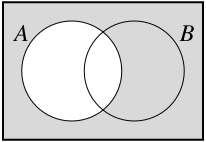
\includegraphics[width=\linewidth]{external/Venn_Diagram_A_complement.pdf}
\end{sbspanel}%
\begin{sbspanel}{0.333333333333333}%
\includegraphics[width=\linewidth]{external/Venn_Diagram_B_complement.pdf}
\end{sbspanel}%
\end{sidebyside}%
\begin{sidebyside}{3}{0}{0}{0}%
\begin{sbspanel}{0.333333333333333}%
%
\begin{equation*}
A \cap B
\end{equation*}
%
\end{sbspanel}%
\begin{sbspanel}{0.333333333333333}%
\par
%
\begin{equation*}
A^{c}
\end{equation*}
%
\end{sbspanel}%
\begin{sbspanel}{0.333333333333333}%
\par
%
\begin{equation*}
B^{c}
\end{equation*}
%
\end{sbspanel}%
\end{sidebyside}%
\tcblower
\end{figureptx}%
As we have discussed, to prove that two sets \(X\) and \(Y\) are equal we prove that each is a subset of the other. The next example provides another illustration of the idea.%
\begin{example}{Example}{}{example-ex_set_eq}%
Let \(A\), \(B\), and \(C\) be sets. We will prove that \(A \cap (B \setminus C) = (A \cap B) \setminus (A \cap C)\).%
\par
To prove this set equality we must prove that \(A \cap (B \setminus C) \subseteq (A \cap B) \setminus (A \cap C)\) and \((A \cap B) \setminus (A \cap C) \subseteq A \cap (B \setminus C)\). We start with \(A \cap (B \setminus C) \subseteq (A \cap B) \setminus (A \cap C)\).%
\par
To prove that \(A \cap (B \setminus C) \subseteq (A \cap B) \setminus (A \cap C)\), we need to demonstrate that every element in \(A \cap (B \setminus C)\) is also in \((A \cap B) \setminus (A \cap C)\). To do this, we select an arbitrary element in \(A \cap (B \setminus C)\) and show that this element is in \((A \cap B) \setminus (A \cap C)\). Let \(x \in A \cap (B \setminus C)\). Then \(x \in A\) and \(x \in B \setminus C\). The fact that \(x \in B \setminus C\) implies that \(x \in B\) but \(x \notin C\). Therefore, \(x \in A\) and \(x \in B\), but \(x \notin C\). This implies that \(x \in A\) and \(x \in B\), but \(x \in A\) and \(x \notin C\). So \(x \in A\) and \(x \in B\), but \(x \notin A \cap C\). We conclude that \(x \in (A \cap B) \setminus (A \cap C)\). This proves that \(A \cap (B \setminus C) \subseteq (A \cap B) \setminus (A \cap C)\).%
\par
For the reverse containment, we let \(y \in (A \cap B) \setminus (A \cap C)\). So \(y \in A \cap B\) but \(y \notin A \cap C\). Since \(y \in A \cap B\), we know that \(y \in A\) and \(y \in B\). The fact that \(y \notin A \cap C\) means that \(y \notin C\). So \(y \in A\), \(y \in B\), and \(y \notin C\). Thus, \(y \in A\) and \(y \in B \setminus C\). We conclude that \(y \in A \cap (B \setminus C)\), which shows that \((A \cap B) \setminus (A \cap C) \subseteq A \cap (B \setminus C)\). The two containments, \(A \cap (B \setminus C) \subseteq (A \cap B) \setminus (A \cap C)\) and \((A \cap B) \setminus (A \cap C) \subseteq A \cap (B \setminus C)\) demonstrate that \(A \cap (B \setminus C) = (A \cap B) \setminus (A \cap C)\).%
\end{example}
We will use the ideas in \hyperref[activity-act_set_equality]{Activity~{\xreffont\ref{activity-act_set_equality}}} and \hyperref[example-ex_set_eq]{Example~{\xreffont\ref{example-ex_set_eq}}} to prove set equalities throughout this text. The next activity will provide some additional practice.%
\begin{activity}{Activity}{}{activity-act_sets_1}%
In this activity we work with unions, intersections, and complements of sets. Let \(A\) and \(B\) be sets.%
\begin{enumerate}[font=\bfseries,label=(\alph*),ref=\alph*]%
\item{}Let \(A = \{1,2,3,4,5,6\}\) and \(B = \{2,4,6,8,10\}\), with \(U = \{1,2,3,4,5,6,7,8,9,10\}\).%
\begin{enumerate}[font=\bfseries,label=(\roman*),ref=\theenumi.\roman*]%
\item{}Determine the elements in \(A \cup B\) and \(A \cap B\). What are the elements in \((A \cup B)^c\) and \((A \cap B)^c\)?%
\item{}Determine the elements in \(A^{c} \cup B^{c}\) and \(A^{c} \cap B^{c}\).%
\end{enumerate}%
\item{}Let \(A\) and \(B\) be arbitrary subsets of a universal set \(U\). There are connections between \(A\), \(B\) and their complements, unions, and intersections.%
\begin{enumerate}[font=\bfseries,label=(\roman*),ref=\theenumi.\roman*]%
\item{}Use Venn diagrams to draw \((A \cup B)^c\) and \((A \cap B)^c\).%
\item{}Use the Venn diagrams and the result of (a) to find and prove a relationship between \(A^c\), \(B^c\) and \((A \cup B)^c\).%
\item{}Use the Venn diagrams and the result of (a) to find and prove a relationship between \(A^c\), \(B^c\) and \((A \cap B)^c\).%
\end{enumerate}%
\end{enumerate}%
\end{activity}%
In \hyperref[activity-act_sets_1]{Activity~{\xreffont\ref{activity-act_sets_1}}} we worked with the union and intersection of two sets. There is no reason to restrict these definitions to only two sets, as the next activity illustrates.%
\begin{activity}{Activity}{}{activity-sec_union_int_comp-n}%
\index{indexed family of sets}%
To define an infinite collection of sets we often use what is called an \terminology{indexing set}. An indexing set allows us to consider a collection of objects that are in one-to-one correspondence with a set like the positive integers, or even the real numbers. When using an indexing set, we generally make a statement such as \textasciigrave{}\textasciigrave{}let \(\{A_{\alpha}\}\) for \(\alpha \in I\) be a collection of sets indexed by some set \(I\)". The collection \(\{A_{\alpha}\}_{\alpha \in I}\) is called an \terminology{indexed family of sets}.%
\begin{enumerate}[font=\bfseries,label=(\alph*),ref=\alph*]%
\item{}The set \(I\) could be finite. As an example, let \(A_{n} = \{1, 2, 3, \ldots n\}\) for \(n\) in the set \(I = \{1,2,3, \ldots, 10\}\).%
\begin{enumerate}[font=\bfseries,label=(\roman*),ref=\theenumi.\roman*]%
\item{}What is \(A_5\)? What is \(A_{8}\)?%
\item{}How many sets are in the indexed family \(\{A_n\}_{n \in I}\)?%
\end{enumerate}%
\item{}The indexing set can be infinite. For example, let \(A_{\alpha} = [0, |\alpha|)\) for \(\alpha\) in the set \(\R\) (where \([a,b)\) is the interval consisting of the real numbers \(x\) such that \(a \leq x \lt b\)). In this case, what is \(A_5\)? What is \(A_{\pi}\)? What is \(A_{-\frac{2}{3}}\)?%
\item{}We have defined the union and intersection of two sets. The same idea can be extended to define the union and intersection of an indexed collection of sets.%
\begin{enumerate}[font=\bfseries,label=(\roman*),ref=\theenumi.\roman*]%
\item{}Recall that if \(A\) and \(B\) are sets, the intersection \(A \cap B\) is the set \(\{x \mid x \in A \text{ and }  x \in B\}\). How can we extend this definition from two sets to any collection of sets? In other words, how do we \emph{define}%
\begin{equation*}
\bigcap_{\alpha \in I} A_{\alpha}?
\end{equation*}
In the example in (b), what set is \(\ds \bigcap_{\alpha \in \R} A_{\alpha}\)?%
\item{}Recall that if \(A\) and \(B\) are sets, the union \(A \cup B\) is the set \(\{x \mid x \in A \text{ or }  x \in B\}\). How can we extend this definition from two sets to any collection of sets? In other words, how do we \emph{define}%
\begin{equation*}
\bigcup_{\alpha \in I} A_{\alpha}?
\end{equation*}
In the example in (b), what set is \(\ds \bigcup_{\alpha \in \R} A_{\alpha}\)?%
\end{enumerate}%
\end{enumerate}%
\end{activity}%
These properties \((A \cap B)^c = A^c \cup B^c\) and \((A \cup B)^c = A^c \cap B^c\) that we learned about in \hyperref[activity-act_sets_1]{Activity~{\xreffont\ref{activity-act_sets_1}}} are called DeMorgan's Laws. These laws apply to any union or intersection of sets, finite or infinite. The proofs are left for \hyperlink{exercise-ex_DeMorgan}{Exercise~{\xreffont 4}}.%
\begin{theorem}{Theorem}{DeMorgan's Laws.}{}{theorem-sec_union_int_comp-p}%
Let \(\{A_{\alpha}\}\) is a collection of sets indexed by a set \(I\) in some universal set \(U\). Then%
\begin{enumerate}
\item{}\(\displaystyle \displaystyle \left(\bigcup_{\alpha \in I} A_{\alpha}\right)^c = \bigcap_{\alpha \in I} A_{\alpha}^c\)%
\item{}\(\displaystyle \displaystyle \left(\bigcap_{\alpha \in I} A_{\alpha}\right)^c = \bigcup_{\alpha \in I} A_{\alpha}^c\)%
\end{enumerate}
%
\end{theorem}
\begin{activity}{Activity}{}{activity-sec_union_int_comp-q}%
\begin{enumerate}[font=\bfseries,label=(\alph*),ref=\alph*]%
\item{}Verify DeMorgan's Laws in the specific case of \(A_{\alpha} = \{1, 2, 3, \ldots \alpha\}\) in \(U = \Z\), where \(\alpha\) is any element of the indexing set \(I = \Z^+\).%
\item{}Why should the complement of a union be an intersection and why should the complement of an intersection be a union?%
\par\smallskip%
\noindent\textbf{\blocktitlefont Hint}.\hypertarget{hint-sec_union_int_comp-q-b-b}{}\quad{}Consider the definitions of unions and intersections.%
\end{enumerate}%
\end{activity}%
\end{sectionptx}
%
%
\typeout{************************************************}
\typeout{Section  Cartesian Products of Sets}
\typeout{************************************************}
%
\begin{sectionptx}{Section}{Cartesian Products of Sets}{}{Cartesian Products of Sets}{}{}{section-sec_cart_prod}
The final operation on sets that we discuss is the \terminology{Cartesian product} (or \terminology{cross product}). This is an operation that we have seen before. When we draw the graph of a line \(y = mx+b\) in the plane, we plot the points \((x,mx+b)\). These points are ordered pairs of real numbers. We can extend this idea to any sets.%
\begin{definition}{Definition}{}{definition-sec_cart_prod-c}%
\index{Cartesian product}%
Let \(A\) and \(B\) are sets. The \terminology{Cartesian product} of \(A\) and \(B\) is the set%
\begin{equation*}
A \times B = \{(a,b) \mid a \in A \text{ and }  b \in B\}\text{.}
\end{equation*}
%
\end{definition}
In other words, the Cartesian product of \(A\) and \(B\) is the set of ordered pairs \((a,b)\) with \(a\) coming from \(A\) and \(b\) coming from \(B\). Note that the order is important.%
\begin{activity}{Activity}{}{activity-sec_cart_prod-e}%
\begin{enumerate}[font=\bfseries,label=(\alph*),ref=\alph*]%
\item{}List all of the elements in \(\{\text{ red } , \text{ blue } \} \times \{\text{ car } , \text{ truck } , \text{ van } \}\).%
\item{}If \(A\) has \(m\) elements and \(B\) has \(n\) elements, how many elements does the set \(A \times B\) have? Explain.%
\end{enumerate}%
\end{activity}%
There is no reason to restrict ourselves to a Cartesian product of just two sets. This is an idea that we have encountered before. The Cartesian product \(\R \times \R\) is the standard real plane that we denote as \(\R^2\) and the Cartesian product \(\R \times \R \times \R\) is the three-dimensional real space denoted as \(\R^3\). If we have an indexed collection \(\{X_{i}\}\) of sets, with \(i\) running through the set of positive integers, then we can define the Cartesian product of the sets \(X_{i}\) as the set of infinite sequences \((x_1, x_2, \ldots,
x_n, \ldots)\), where \(x_i \in X_i\) for each \(i \in \Z^+\). We denote this cartesian product as%
\begin{equation*}
\Pi_{i \in \Z^+} X_i = \Pi_{i=1}^{\infty} X_i\text{.}
\end{equation*}
%
\par
The capital pi (\(\Pi\)) is used to represent a product an an analog of the capital sigma (\(\Sigma\)) that is used to represent a sum. We will study sequences in more detail later.%
\par
To conclude this section we summarize some properties of sets. Many of these properties can be extended to arbitrary collections of sets. Most of the proofs are straightforward. The associative and distributive laws are left for \hyperlink{exercise-ex_set_props}{Exercise~{\xreffont 3}}.%
\begin{theorem}{Theorem}{}{}{theorem-sec_cart_prod-i}%
Let \(A\), \(B\), and \(C\) be subsets of a universal set \(U\).%
\begin{descriptionlist}
\begin{dlinarrow}{Properties of the Empty Set}{li-sec_cart_prod-i-a-a-e-a}%
%
\begin{enumerate}[label=\roman*]
\item{}\(\displaystyle A \cap \emptyset = \emptyset\)%
\item{}\(\displaystyle A \cup \emptyset = A\)%
\item{}\(\displaystyle A-\emptyset = A\)%
\item{}\(\displaystyle \emptyset^c = U\)%
\end{enumerate}
%
\end{dlinarrow}%
\begin{dlinarrow}{Properties of the Universal Set}{li-sec_cart_prod-i-a-a-e-b}%
%
\begin{enumerate}[label=\roman*]
\item{}\(\displaystyle A \cap U = A\)%
\item{}\(\displaystyle A \cup U = U\)%
\item{}\(\displaystyle A-U = \emptyset\)%
\item{}\(\displaystyle U^c = \emptyset\)%
\end{enumerate}
%
\end{dlinarrow}%
\begin{dlinarrow}{Idempotent Laws}{li-sec_cart_prod-i-a-a-e-c}%
%
\begin{enumerate}[label=\roman*]
\item{}\(\displaystyle A \cap A = A\)%
\item{}\(\displaystyle A \cup A = A\)%
\end{enumerate}
%
\end{dlinarrow}%
\begin{dlinarrow}{Commutative Laws}{li-sec_cart_prod-i-a-a-e-d}%
%
\begin{enumerate}[label=\roman*]
\item{}\(\displaystyle A \cap B = B \cap A\)%
\item{}\(\displaystyle A \cup B = B \cup A\)%
\end{enumerate}
%
\end{dlinarrow}%
\begin{dlinarrow}{Associative Laws}{li-sec_cart_prod-i-a-a-e-e}%
%
\begin{enumerate}[label=\roman*]
\item{}\(\displaystyle (A \cap B) \cap C = A \cap (B \cap C)\)%
\item{}\(\displaystyle (A \cup B) \cup C = A \cup (B \cup C)\)%
\end{enumerate}
%
\end{dlinarrow}%
\begin{dlinarrow}{Distributive Laws}{li-sec_cart_prod-i-a-a-e-f}%
%
\begin{enumerate}[label=\roman*]
\item{}\(\displaystyle A \cap (B \cup C) = (A \cap B) \cup (A \cap C)\)%
\item{}\(\displaystyle A \cup (B \cap C) = (A \cup B) \cap (A \cup C)\)%
\end{enumerate}
%
\end{dlinarrow}%
\begin{dlinarrow}{Basic Properties}{li-sec_cart_prod-i-a-a-e-g}%
%
\begin{enumerate}[label=\roman*]
\item{}\(\displaystyle \left(A^c\right)^c = A\)%
\item{}\(\displaystyle A - B = A \cap B^c\)%
\end{enumerate}
%
\end{dlinarrow}%
\begin{dlinarrow}{Subsets and Complements}{li-sec_cart_prod-i-a-a-e-h}%
\(\displaystyle A \subseteq B \text{ if and only if } B^c \subseteq A^c\)%
\end{dlinarrow}%
\end{descriptionlist}
%
\end{theorem}
\end{sectionptx}
%
%
\typeout{************************************************}
\typeout{Section  Summary}
\typeout{************************************************}
%
\begin{sectionptx}{Section}{Summary}{}{Summary}{}{}{section-sec_sets_summ}
Important ideas that we discussed in this section include the following.%
\begin{itemize}[label=\textbullet]
\item{}We can consider a set to be a well-defined collection of elements.%
\item{}A subset of a set is any collection of elements from that set. That is, a subset \(S\) of a set \(X\) is a set with the property that if \(s \in S\), then \(s \in X\).%
\item{}If \(X\) and \(Y\) are sets, then the union \(X \cup Y\) is the set%
\begin{equation*}
X \cup Y = \{z \mid z \in X \text{ or }  z \in Y\}\text{.}
\end{equation*}
The union of an arbitrary collection \(\{X_{\alpha}\}\) of sets for \(\alpha\) in some indexing set \(I\) is the set%
\begin{equation*}
\bigcup_{\alpha \in I} X_{\alpha} = \{z \mid z \in X_{\beta} \text{ for some }  \beta \in I\}\text{.}
\end{equation*}
%
\item{}If \(X\) and \(Y\) are sets, then the intersection \(X \cap Y\) is the set%
\begin{equation*}
X \cap Y = \{z \mid z \in X \text{ and }  z \in Y\}\text{.}
\end{equation*}
The intersection of an arbitrary collection \(\{X_{\alpha}\}\) of sets for \(\alpha\) in some indexing set \(I\) is the set%
\begin{equation*}
\bigcap_{\alpha \in I} X_{\alpha} = \{z \mid z \in X_{\beta} \text{ for all }  \beta \in I\}\text{.}
\end{equation*}
%
\item{}If \(X\) is a set and \(A\) is a subset of \(X\), then the complement of \(A\) in \(X\) is the set%
\begin{equation*}
A^c = \{x \in X \mid x \notin A\}\text{.}
\end{equation*}
%
\item{}If \(\{X_{i}\}\) is a collection of sets with \(i\) in some indexing set \(I\), where \(I\) is finite or \(I\) is the set of positive integers, the Cartesian product \(\Pi_{i \in I} X_i\) of the sets \(X_{i}\) as the set of all ordered tuples of the form \((x_i)\) where \(i \in I\).%
\end{itemize}
%
\end{sectionptx}
%
%
\typeout{************************************************}
\typeout{Exercises  Exercises}
\typeout{************************************************}
%
\begin{exercises-section}{Exercises}{Exercises}{}{Exercises}{}{}{exercises-sec_sets_exer}
\begin{divisionexercise}{1}{}{}{exercise-sec_sets_exer-a}%
Let \(A\), \(B\), and \(C\) be subsets of a set \(X\). Express each of the following sets in mathematical notation using the symbols \(\cup\), \(\cap\), and \(\setminus\).%
\begin{enumerate}[font=\bfseries,label=(\alph*),ref=\alph*]%
\item{}The elements of \(X\) that belong to \(A\) and \(B\), but not \(C\).%
\item{}The elements of \(X\) that belong to \(C\) and either \(A\) or \(B\).%
\item{}The elements of \(X\) that belong to \(A\) but not to both \(B\) and \(C\).%
\item{}The elements of \(X\) that belong to none of the sets \(A\), \(B\), and \(C\).%
\item{}The elements of \(X\) that fail to belong to at least two of the sets \(A\), \(B\), and \(C\).%
\item{}The elements of \(X\) that fail to belong to at most one of the sets \(A\), \(B\), and \(C\).%
\end{enumerate}%
\end{divisionexercise}%
\begin{divisionexercise}{2}{}{}{exercise-sec_sets_exer-b}%
Let \(X \subset Y \subset Z\). Prove or disprove.%
\begin{enumerate}[font=\bfseries,label=(\alph*),ref=\alph*]%
\item{}\(C_Y(X) \subset C_Z(X)\).%
\item{}\(Z \setminus (Y \setminus X) = X \cup (Z \setminus Y)\).%
\end{enumerate}%
\end{divisionexercise}%
\begin{divisionexercise}{3}{}{}{exercise-ex_set_props}%
Let \(A\) and \(B\) be subsets of a universal set \(U\). Prove the associative and distributive laws. That is, prove each of the following.%
\begin{enumerate}[font=\bfseries,label=(\alph*),ref=\alph*]%
\item{}\((A \cap B) \cap C = A \cap (B \cap C)\)%
\item{}\((A \cup B) \cup C = A \cup (B \cup C)\)%
\item{}\(A \cap (B \cup C) = (A \cap B) \cup (A \cap C)\) \textbackslash{}item\(A \cup (B \cap C) = (A \cup B) \cap (A \cup C)\)%
\end{enumerate}%
\end{divisionexercise}%
\begin{divisionexercise}{4}{}{}{exercise-ex_DeMorgan}%
Prove DeMorgan's Laws. That is, let \(\{A_{\alpha}\}\) be a collection of sets indexed by a set \(I\) in some universal set \(U\). Prove that%
\begin{enumerate}[font=\bfseries,label=(\alph*),ref=\alph*]%
\item{}\(\displaystyle \left(\bigcup_{\alpha \in I} A_{\alpha}\right)^c = \bigcap_{\alpha \in I} A_{\alpha}^c\)%
\item{}\(\displaystyle \left(\bigcap_{\alpha \in I} A_{\alpha}\right)^c = \bigcup_{\alpha \in I} A_{\alpha}^c\)%
\end{enumerate}%
\end{divisionexercise}%
\begin{divisionexercise}{5}{}{}{exercise-sec_sets_exer-e}%
What familiar set is \(\emptyset \times A\) for any set \(A\)? Explain.%
\end{divisionexercise}%
\begin{divisionexercise}{6}{}{}{exercise-ex_power_set}%
\index{power set}%
If \(A\) is a set, the power set of \(A\), denoted \(2^A\) is the collection of all subsets of \(A\).%
\begin{enumerate}[font=\bfseries,label=(\alph*),ref=\alph*]%
\item{}List the elements of \(\ds 2^{\{1,2\}}\).%
\item{}If \(A\) is a set with three elements, how many elements are in \(2^A\)?%
\item{}If \(A\) is a set with \(n\) elements, make a conjecture about the number of elements in \(2^A\). Prove your conjecture?%
\end{enumerate}%
\end{divisionexercise}%
\begin{divisionexercise}{7}{}{}{exercise-sec_sets_exer-g}%
If \(A\) is a set, the power set of \(A\), denoted \(2^A\) is the collection of all subsets of \(A\). (See \hyperlink{exercise-ex_power_set}{Exercise~{\xreffont 6}}.) Critique each of the following statements. Doe the statement make sense or not? If not, explain why and then correct the statement to something that is true (and non-trivial).%
\begin{enumerate}[font=\bfseries,label=(\alph*),ref=\alph*]%
\item{}If \(A\) is a set, then \(A \in 2^A\).%
\item{}If \(A\) is a set, then \(A \subset 2^A\).%
\item{}If \(A\) is a set, then \(\{A\} \subset 2^A\).%
\item{}If \(A\) is a set, then \(\emptyset \in 2^A\).%
\item{}If \(A\) is a set, then \(\emptyset \subset 2^A\).%
\item{}If \(A\) and \(B\) are sets and \(A \subseteq B\), then \(2^A \subseteq 2^B\).%
\end{enumerate}%
\end{divisionexercise}%
\begin{divisionexercise}{8}{}{}{exercise-sec_sets_exer-h}%
Let \(A\) and \(B\) be sets, both of which have at least two distinct members. Prove that there is a subset \(W \subset A \times B\) that is not the Cartesian product of a subset of \(A\) with a subset of \(B\). [Thus, not every subset of a Cartesian product is the Cartesian product of a pair of subsets.]%
\end{divisionexercise}%
\begin{divisionexercise}{9}{}{}{exercise-sec_sets_exer-i}%
Let \(I\) be the set of real numbers that are greater than \(0\). For each \(x \in I\), let \(A_x\) be the open interval \((0,x)\). Prove that \(\bigcap_{x \in I} A_x = \emptyset\), \(\bigcup_{x \in I} A_x = I\). For each \(x \in I\), let \(B_x\) be the closed interval \([0,x]\). Prove that \(\bigcap_{x \in I} B_x = \{0\}\), \(\bigcup_{x \in I} B_x = I \cup \{0\}\).%
\end{divisionexercise}%
\begin{divisionexercise}{10}{}{}{exercise-sec_sets_exer-j}%
For each of the following, answer true if the statement is always true. If the statement is only sometimes true or never true, answer false and provide a concrete example to illustrate that the statement is false. If a statement is true, explain why. As an example of a true statement, consider the statement%
\begin{quote}%
Let \(A\), \(B\), and \(C\) be sets such that \(A \cap B = A \cap C\) and \(A \cap B \neq \emptyset\).%
\end{quote}
Then \(B \cap C \neq \emptyset\). We can justify the truth of this statement with a short argument. Since \(A \cap B \neq \emptyset\), there is an element \(x \in A \cap B\). Then \(x \in B\). Since \(A \cap B = A \cap C\), we also must have \(x \in A \cap C\), which implies that \(x \in C\). Thus, \(x \in B \cap C\) and \(B \cap C \neq \emptyset\). As an example of a false statement, consider the statement%
\begin{quote}%
Let \(A\), \(B\), and \(C\) be sets such that \(A \cap B = A \cap C\).%
\end{quote}
Then \(B = C\). We can show that this statement is false by providing a counterexample. For example, let \(A = \{0,1\}\), \(B=\{1\}\), and \(C = \{1,2\}\). Then \(A \cap B = \{1\} = A \cap C\), but \(B \neq C\).%
\begin{enumerate}[font=\bfseries,label=(\alph*),ref=\alph*]%
\item{}If \(A\), \(B\), and \(C\) are sets and \(A \subseteq B\) and \(A \subseteq C\), then \(A \subseteq (B \cap C)\).%
\item{}If \(A\), \(B\), and \(C\) are sets and \(A \subseteq C\) and \(B \subseteq C\), then \((A \cup B) \subseteq C\).%
\item{}If \(A\) and \(B\) are subsets of a set \(X\) and \(A \subseteq B\), then \((X \setminus A) \subseteq (X \setminus B)\).%
\item{}If \(A\) and \(B\) are subsets of a set \(X\) and \(A \subseteq B\), then \((X \setminus B) \subseteq (X \setminus A)\).%
\item{}If \(A\) and \(B\) are sets, then \((A \cup B) \setminus B = A\).%
\item{}If \(A\) and \(B\) are sets, then \(A \setminus (A \setminus B) = B\).%
\item{}If \(A\), \(B\), and \(C\) are sets, then \(A \cap (B \setminus C) = (A \cap B) \setminus (A \cap C)\).%
\item{}If \(A\) and \(C\) are subsets of a set \(X\), then \((A \setminus C) = A \cap (X \setminus C)\).%
\item{}There are no elements of the set \(\{\emptyset\}\).%
\item{}There are two distinct objects that belong to the set \(\{\emptyset, \{\emptyset\}\}\).%
\end{enumerate}%
\end{divisionexercise}%
\end{exercises-section}
\end{chapterptx}
 %
%
\typeout{************************************************}
\typeout{Chapter 2 Functions}
\typeout{************************************************}
%
\begin{chapterptx}{Chapter}{Functions}{}{Functions}{}{}{chapter-chap_functions}
\renewcommand*{\chaptername}{Chapter}
\begin{objectives}{Focus Questions}{objectives-chap_functions-b}
%
\begin{itemize}[label=\textbullet]
\item{}What is a function?%
\item{}What is the domain of a function?%
\item{}What is the difference between the range and codomain of a function?%
\item{}What does it mean for a function to be an injection? A surjection?%
\item{}When and how is the composite of two functions defined?%
\item{}When and how is the inverse of a function defined?%
\item{}What do we mean by the image and inverse image of a set under a function?%
\item{}What properties relate images and inverse images of sets and set unions?%
\end{itemize}
\end{objectives}
%
%
\typeout{************************************************}
\typeout{Section  Introduction}
\typeout{************************************************}
%
\begin{sectionptx}{Section}{Introduction}{}{Introduction}{}{}{section-sec_func_intro}
Many topological properties are defined using continuous functions. We will focus on continuity later \textemdash{} for now we review some important concepts related to functions. Much of this should be familiar, but some might be new.%
\par
First we present the basic definitions. Much of our previous work has probably been with functions that map from the reals to the reals, but we will be considering functions form a more general perspective. We start with a formal definition of a function.%
\begin{definition}{Definition}{}{definition-def_function}%
\index{function}%
A \terminology{function} \(f\) from a nonempty set \(A\) to a set \(B\) is a collection of ordered pairs \((a,b)\) so that%
\begin{itemize}[label=\textbullet]
\item{}for each \(a \in A\) there is a pair \((a,b)\) in \(f\), and%
\item{}if \((a,b)\) and \((a,b')\) are in \(f\), then \(b=b'\).%
\end{itemize}
%
\end{definition}
Note that the first property is an existence property \textemdash{} that if \(a \in A\) then there is an element \(b\) in \(B\) that matches up with \(a\). This first property also says that every element in \(A\) is used, or that every element in \(A\) is paired with an element in \(B\), and the element in \(B\) depends on the element in \(A\) that is chosen. The second property is a uniqueness one \textemdash{} that there is only one element \(b\) in \(B\) that is paired with a given element \(a\) in \(A\).%
\par
We generally use an alternate notation for a function. If \((a,b)\) is an element of a function \(f\), we write%
\begin{equation*}
f(a)=b\text{,}
\end{equation*}
and in this way we think of \(f\) as a mapping from the set \(A\) to the set \(B\). We indicate that \(f\) is a mapping from set \(A\) to set \(B\) with the notation%
\begin{equation*}
f : A \to B\text{.}
\end{equation*}
%
\par
If \(f\) maps the element \(a \in A\) to the element \(b \in B\) we also use the notation%
\begin{equation*}
f : a \mapsto b\text{.}
\end{equation*}
%
\par
There is some familiar terminology and notation associated with functions. Let \(f\) be a function from a set \(A\) to a set \(B\).%
\begin{itemize}[label=\textbullet]
\item{}The set \(A\) is called the \terminology{domain} \index{function!domain} of \(f\), and we write \(\text{ dom } (f) = A\).%
\item{}The set \(B\) is called the \terminology{codomain} \index{function!codomain} of \(f\), and we write \(\text{ codom } (f) = B\).%
\item{}The subset \(\{f(a) \mid a \in A\}\) of \(B\) is called the \terminology{range} \index{function!range} of \(f\), which we denote by \(\text{ range } (f)\).%
\item{}If \(a \in A\), then \(f(a)\) is the \terminology{image} \index{image of an element} of \(a\) under \(f\). Since each \(a\) in \(A\) is paired with a unique \(b \in B\), there is only one image of \(a\) under \(f\). That is why it is appropriate to use the work ``the'' when referring to the image of an element.%
\item{}If \(b \in B\) and \(b = f(a)\) for some \(a \in A\), then \(a\) is called a \terminology{preimage} \index{preimage of an element} of \(b\). For a given \(b \in B\), there may be many different preimages of \(b\), no preimages of \(b\), or just one preimage of \(b\). It can be instructive to construct examples of each situation. The fact that a preimage of an element \(b\) may not be unique is the reason we use the word ``a'' when referring to a preimage.%
\end{itemize}
%
\par
Knowing the domains and codomains is very important when working with functions, and we will pay a lot of attention to these sets.%
\par
We have likely been exposed to one-to-one and onto function in our past mathematical experiences. One-to-one functions (or injections) and onto functions (or surjections) are special types of functions and we present their definitions here.%
\begin{definition}{Definition}{}{definition-sec_func_intro-k}%
\index{function!injection}%
\index{function!surjection}%
\index{function!bijection}%
Let \(f\) be a function from a set \(A\) to a set \(B\).%
\begin{enumerate}
\item{}The function \(f\) is an \terminology{injection} if, whenever \((a,b)\) and \((a',b)\) are in \(f\), then \(a=a'\). Alternatively, using the function notation, \(f\) is an injection if \(f(a)=f(a')\) implies \(a=a'\).%
\item{}The function \(f\) is a \terminology{surjection} if, whenever \(b \in B\), then there is an \(a \in A\) so that \((a,b)\) is in \(f\). Alternatively, using the function notation, \(f\) is a surjection if for each \(b \in B\) there exists an \(a \in A\) so that \(f(a)=b\).%
\item{}The function \(f\) is a \terminology{bijection} if \(f\) is both an injection and a surjection.%
\end{enumerate}
%
\end{definition}
\begin{exploration}{Preview Activity}{}{exploration-sec_func_intro-l}%
We often define functions with rules, but functions can also be defined by tables or graphs. We will work with functions defined by rules in this activity. The goal of this activity is to illustrate why the domain and the codomain are just as important as the rule defining the outputs when want to determine if a function is one-to-one and\slash{}or onto. As an example, let \(f(x) = x^2+1\). (Note that \(f\) is the function and \(f(x)\) is the image of \(x\) under \(f\).) Notice that%
\begin{equation*}
f(2) = 5 \text{ and }  f(-2) = 5\text{.}
\end{equation*}
%
\par
This observation is enough to prove that the function \(f\) is not an injection since we can see that there exist two different inputs that produce the same output.%
\par
Since \(f(x) = x^2 + 1\), we know that \(f(x) \geq 1\) for all \(x \in \R\). This implies that the function \(f\) is not a surjection. For example, \(-2\) is in the codomain of \(f\) and \(f(x) \neq -2\) for all \(x\) in the domain of \(f\).%
\begin{enumerate}[font=\bfseries,label=(\alph*),ref=\alph*]%
\item{}We can change the domain of a function so that the function is defined on a subset of the original domain. Such a function is called a restriction.%
\begin{definition}{Definition}{}{definition-sec_func_intro-l-b-a-b}%
\index{function!restriction}%
Let \(f\) be a function from a set \(A\) to a set \(B\) and let \(C\) be a subset of \(A\). The \terminology{restriction} of \(f\) to \(C\) is the function \(F: C \to B\) satisfying%
\begin{equation*}
F(c) = f(c) \text{ for all }  c \in C\text{.}
\end{equation*}
%
\end{definition}
A notation used for the restriction is also \(F = f\mid_C\). We also call \(f\) an \terminology{extension} of \(F\). Let \(f: \R \to \R\) be defined by \(f(x) = x^2+1\), and let \(h = f \mid_{\R^+}\), where \(\R^+\) is the set of positive real numbers. So \(h\) has the same codomain as \(f\), but a different domain.%
\begin{enumerate}[font=\bfseries,label=(\roman*),ref=\theenumi.\roman*]%
\item{}Show that \(h\) is an injection.%
\item{}Is \(h\) a surjection? Justify your conclusion.%
\end{enumerate}%
\item{}Let \(T = \{y \in \R \mid y \geq 1\}\), and let \(F: \R \to T\) be defined by \(F(x) = f(x)\). Notice that the function \(F\) uses the same formula as the function \(f\) and has the same domain as \(f\), but has a different codomain than \(f\).%
\begin{enumerate}[font=\bfseries,label=(\roman*),ref=\theenumi.\roman*]%
\item{}Explain why \(F\) is not an injection.%
\item{}Is \(F\) a surjection? Justify your conclusion.%
\end{enumerate}%
\item{}Let \(\R^*= \{x \in \R \mid x \geq 0\}\). Define \(g : \R^* \to T\) by \(g(x) = x^2 + 1\).%
\begin{enumerate}[font=\bfseries,label=(\roman*),ref=\theenumi.\roman*]%
\item{}Prove or disprove: the function \(g\) is an injection.%
\item{}Prove or disprove: the function \(g\) is a surjection.%
\end{enumerate}%
\end{enumerate}%
\end{exploration}%
In our preview activity, the same mathematical formula was used to determine the outputs for the functions. However:%
\begin{itemize}[label=\textbullet]
\item{}One of the functions was neither an injection nor a surjection.%
\item{}One of the functions was not an injection but was a surjection.%
\item{}One of the functions was an injection but was not a surjection.%
\item{}One of the functions was both an injection and a surjection.%
\end{itemize}
%
\par
This illustrates the important fact that whether a function is injective or surjective not only depends on the formula that defines the output of the function but also on the domain and codomain of the function.%
\par
An important special function that is always an injection and surjection is the \terminology{identity} function \index{function!identity} on a set. If \(A\) is a set, the identity function on \(A\) is denoted as \(i_A\), and \(i_A(a) = a\) for every \(a \in A\).%
\end{sectionptx}
%
%
\typeout{************************************************}
\typeout{Section  Composites of Functions}
\typeout{************************************************}
%
\begin{sectionptx}{Section}{Composites of Functions}{}{Composites of Functions}{}{}{section-sec_comp_func}
In our past mathematical experiences, we have often added and multiplied functions together (e.g., if \(f(x) = x^2\) and \(g(x) = x+1\) map from \(\R\) to \(\R\), then \((fg)(x) = x^2(x+1)\) and \((f+g)(x) = x^2+(x+1)\)). In topology, we generally don't care about any algebraic structure a set might have, so we will move away from sums and products, and focus on compositions of functions.%
\par
The basic idea of function composition is that, when possible, the output of a function \(f\) is used as the input of a function \(g\). The resulting function can be referred to as ``\(f\) followed by \(g\)'' and is called the composite of \(f\) with \(g\). The notation we use is \(g \circ f\) (note the order \textemdash{} \(f\) is applied first). For example, if%
\begin{equation*}
f(x) = 3x^2 + 2 \text{ and }  g(x) = \sin(x)\text{,}
\end{equation*}
both mapping \(\R\) to \(\R\), then we can compute \((g \circ f)(x)\) as follows:%
\begin{equation*}
(g \circ f)(x) = g(f(x)) = g(3x^2 + 2) = \sin\left(3x^2 + 2\right)\text{.}
\end{equation*}
%
\par
In this case, \(f(x)\), the output of the function \(f\), was used as the input for the function \(g\). This idea motivates the formal definition of the composition of two functions.%
\begin{definition}{Definition}{}{definition-sec_comp_func-e}%
\index{composition of functions}%
Let \(A\), \(B\), and \(C\) be nonempty sets, and let \(f : A \to B\) and \(g : B \to C\) be functions. The \terminology{composite} of \(f\) and \(g\) is the function \(g \circ f : A \to C\) defined by%
\begin{equation*}
(g \circ f)(x) = g(f(x))
\end{equation*}
for all \(x \in A\)%
\end{definition}
We refer to the function \(g \circ f\) as a composite function, and we read \((g \circ f)(x)\) as ``\(g\) of \(f\)'' of \(x\).%
\begin{activity}{Activity}{}{activity-act_functions_1}%
Let \(A = \{1, 2, 3\}\), \(B = \{a, b, c, d\}\), and \(C = \{\alpha, \beta, \gamma\}\). Define \(f : A \to B\), \(g : A \to B\), and \(h : B \to C\) by%
\begin{equation*}
f(1) = b, \ f(2) = c, \  f(3) = a\text{,}
\end{equation*}
%
\begin{equation*}
g(1) = d, \ g(2) = c, \  g(3) = d, \text{ and }
\end{equation*}
%
\begin{equation*}
h(a) = \gamma, \ h(b) = \alpha, \ h(c) = \beta,  \ h(d) = \alpha\text{.}
\end{equation*}
%
\begin{enumerate}[font=\bfseries,label=(\alph*),ref=\alph*]%
\item{}Find the images of the elements in \(A\) under the function \(h \circ f\).%
\item{}Find the images of the elements in \(A\) under the function \(h \circ g\).%
\item{}Are any of \(f\), \(g\), and \(h\) injections? Are any of \(f\), \(g\), and \(h\) surjections?%
\item{}Is \(h \circ f\) an injection? Is \(h \circ f\) a surjection? Explain.%
\item{}Is \(h \circ g\) an injection? Is \(h \circ g\) a surjection? Explain.%
\end{enumerate}%
\end{activity}%
In \hyperref[activity-act_functions_1]{Activity~{\xreffont\ref{activity-act_functions_1}}}, we asked questions about whether certain composite functions were injections and\slash{}or surjections. In mathematics, it is typical to explore whether certain properties of an object transfer to related objects. In particular, we might want to know whether or not the composite of two injective functions is also an injection. (Of course, we could ask a similar question for surjections.) These questions are explored in the next activity.%
\begin{activity}{Activity}{}{activity-act_composition2}%
Let the sets \(A\), \(B\), \(C\), and \(D\) be as follows:%
\begin{equation*}
A = \{ a, b, c \},  B = \{p, q, r\},  C = \{u, v, w, x \},  \text{ and }   D = \{u, v \}\text{.}
\end{equation*}
%
\begin{enumerate}[font=\bfseries,label=(\alph*),ref=\alph*]%
\item{}Construct a function \(f : A \to B\) that is an injection and a function \(g : B \to C\) that is an injection. In this case, is the composite function \(g \circ f : A \to C\) an injection? Explain.%
\item{}Construct a function \(f : A \to B\) that is a surjection and a function \(g : B \to D\) that is a surjection. In this case, is the composite function \(g \circ f : A \to D\) a surjection? Explain.%
\item{}Construct a function \(f : A \to B\) that is a bijection and a function \(g : B \to A\) that is a bijection. In this case, is the composite function \(g \circ f : A \to A\) a bijection? Explain.%
\end{enumerate}%
\end{activity}%
In \hyperref[activity-act_composition2]{Activity~{\xreffont\ref{activity-act_composition2}}}, we explored some properties of composite functions related to injections, surjections, and bijections. The following theorem summarizes the results that these explorations were intended to illustrate.%
\begin{theorem}{Theorem}{}{}{theorem-thm_compositefunctions}%
Let \(A\), \(B\), and \(C\) be nonempty sets, and assume that \(f : A \to B\) and \(g : B \to C\).%
\begin{enumerate}
\item\hypertarget{li-thm_compositefunctions1}{}If \(f\) and \(g\) are both injections, then \((g \circ f) : A \to C\) is an injection.%
\item\hypertarget{li-thm_compositefunctions2}{}If \(f\) and \(g\) are both surjections, then \((g \circ f) : A \to C\) is a surjection.%
\item\hypertarget{li-thm_compositefunctions3}{}If \(f\) and \(g\) are both bijections, then \((g \circ f) : A \to C\) is a bijection.%
\end{enumerate}
%
\end{theorem}
\begin{activity}{Activity}{}{activity-sec_comp_func-l}%
\begin{enumerate}[font=\bfseries,label=(\alph*),ref=\alph*]%
\item{}Prove part (1) of \hyperref[theorem-thm_compositefunctions]{Theorem~{\xreffont\ref{theorem-thm_compositefunctions}}}.%
\item{}Prove part (2) of \hyperref[theorem-thm_compositefunctions]{Theorem~{\xreffont\ref{theorem-thm_compositefunctions}}}.%
\item{}Why is the proof of part (3) of \hyperref[theorem-thm_compositefunctions]{Theorem~{\xreffont\ref{theorem-thm_compositefunctions}}} a direct consequence of parts (1) and (2)?%
\end{enumerate}%
\end{activity}%
\end{sectionptx}
%
%
\typeout{************************************************}
\typeout{Section  Inverse Functions}
\typeout{************************************************}
%
\begin{sectionptx}{Section}{Inverse Functions}{}{Inverse Functions}{}{}{section-sec_inv_func}
Now that we have studied composite functions, we will move on to consider another important idea: the inverse of a function. In previous mathematics courses, you probably learned that the exponential function (with base \(e\)) and the natural logarithm functions are inverses of each other. You may have seen this relationship expressed as follows: For each \(x \in \R\) with \(x \gt 0\) and for each \(y \in \R\),%
\par
\(y = \ln(x)\) if and only if \(x = e^y\). Notice that \(x\) is the input and \(y\) is the output for the natural logarithm function if and only if \(y\) is the input and \(x\) is the output for the exponential function. In essence, the inverse function (in this case, the exponential function) reverses the action of the original function (in this case, the natural logarithm function). In terms of ordered pairs (input-output pairs), this means that if \(( {x, y} )\) is an ordered pair for a function, then \(( {y, x} )\) is an ordered pair for its inverse. The idea of reversing the roles of the first and second coordinates is the basis for our definition of the inverse of a function.%
\begin{definition}{Definition}{}{definition-sym_finverse}%
\index{function!inverse}%
Let \(f : A \to B\) be a function. The \terminology{inverse} of \(f\), denoted by \(f^{ - 1}\), is the set of ordered pairs%
\begin{equation*}
f^{ - 1}  = \left\{ { {( {b, a} ) \in B \times A} \mid ( {a, b} ) \in f} \right\}\text{.}
\end{equation*}
%
\end{definition}
Notice that this definition does not state that \(f^{-1}\) is a function. Rather, \(f^{-1}\) is simply a subset of \(B \times A\). In \hyperref[activity-prog_exploringinverse]{Activity~{\xreffont\ref{activity-prog_exploringinverse}}}, we will explore the conditions under which the inverse of a function \(f: A \to B\) is itself a function from \(B\) to \(A\).%
\begin{activity}{Activity}{}{activity-prog_exploringinverse}%
Let \(A = \left\{ {a, b, c} \right\}\), \(B = \left\{ {a,b,c,d} \right\}\), and \(C = \left\{ {p, q, r} \right\}\). Define%
\begin{align*}
f: A \amp \to C \text{ by} \amp g: A \amp \to C \text{ by} \amp h: B \amp \to C \text{ by}\\
f( a ) \amp = r \amp g( a ) \amp = p \amp h( a ) \amp = p\\
f( b ) \amp = p \amp g( b ) \amp = q \amp h( b ) \amp = q\\
f( c ) \amp = q \amp g( c ) \amp = p \amp h( c ) \amp = r\\
\amp \amp \amp \amp h ( d ) \amp = q
\end{align*}
%
\begin{enumerate}[font=\bfseries,label=(\alph*),ref=\alph*]%
\item{}Determine the inverse of each function as a set of ordered pairs.%
\item{}\begin{enumerate}[font=\bfseries,label=(\roman*),ref=\theenumi.\roman*]%
\item{}Is \(f^{ - 1}\) a function from \(C\) to \(A\)? Explain.%
\item{}Is \(g^{ - 1}\) a function from \(C\) to \(A\)? Explain.%
\item{}Is \(h^{ - 1}\) a function from \(C\) to \(B\)? Explain.%
\end{enumerate}%
\item\label{task-A_exploringinverse3}Make a conjecture about what conditions on a function \(F: S \to T\) will ensure that its inverse is a function from \(T\) to \(S\).%
\end{enumerate}%
\end{activity}%
The result of the \hyperref[activity-prog_exploringinverse]{Activity~{\xreffont\ref{activity-prog_exploringinverse}}} should have been the following theorem.%
\begin{theorem}{Theorem}{}{}{theorem-T_inverseandbijection}%
Let \(A\) and \(B\) be nonempty sets, and let \(f: A \to B\). The inverse of \(f\) is a function from \(B\) to \(A\) if and only if \(f\) is a bijection.%
\end{theorem}
The proof of \hyperref[theorem-T_inverseandbijection]{Theorem~{\xreffont\ref{theorem-T_inverseandbijection}}} is outlined in the following activity.%
\begin{activity}{Activity}{}{activity-sec_inv_func-j}%
\hyperref[theorem-T_inverseandbijection]{Theorem~{\xreffont\ref{theorem-T_inverseandbijection}}} is a biconditional statement, so we need to prove both directions. Let \(A\) and \(B\) be nonempty sets, and let \(f: A \to B\).%
\begin{enumerate}[font=\bfseries,label=(\alph*),ref=\alph*]%
\item{}Assume that  \(f\)  is a bijection. We will prove that \(f^{-1}\) is a function, that is that \(f^{-1}\) satisfies the conditions of \hyperref[definition-def_function]{Definition~{\xreffont\ref{definition-def_function}}}.%
\begin{enumerate}[font=\bfseries,label=(\roman*),ref=\theenumi.\roman*]%
\item{}Let \(b \in B\). What property does \(f\) have that ensures that \((b,a) \in f^{-1}\) for some \(a \in A\)? What conclusion can we draw about \(f^{-1}\)?%
\item{}Now let \(b \in B\), \(a_1 , a_2  \in A\) and assume that%
\begin{equation*}
( {b, a_1 } ) \in f^{ - 1} \text{ and }  ( {b, a_2 } ) \in f^{-1}\text{.}
\end{equation*}
What does this tell us about elements that must be in \(f\)? What property of \(f\) ensures that \(a_1=a_2\)? What conclusion can we draw about \(f^{-1}\)?%
\end{enumerate}%
\item{}Now assume that \(f^{-1}\) is a function from \(B\) to \(A\). We will prove that \(f\) is a bijection.%
\begin{enumerate}[font=\bfseries,label=(\roman*),ref=\theenumi.\roman*]%
\item{}What does it take to prove that \(f\) is an injection? Use the fact that \(f^{-1}\) is a function to prove that \(f\) is an injection.%
\item{}What does it take to prove that \(f\) is a surjection? Use the fact that \(f^{-1}\) is a function to prove that \(f\) is a surjection.%
\end{enumerate}%
\end{enumerate}%
\end{activity}%
In the situation where \(f: A \to B\) is a bijection and \(f^{-1}\) is a function from \(B\) to \(A\), we can write \(f^{-1} : B \to A\). In this case, we frequently say that \(f\) is an \terminology{invertible function}, and we usually do not use the ordered pair representation for either \(f\) or \(f^{-1}\). Instead of writing \(( {a, b} ) \in f\), we write \(f( a ) = b\), and instead of writing \(( {b, a} ) \in f^{-1}\), we write \(f^{-1} ( b ) = a\). Using the fact that \(( {a, b} ) \in f\) if and only if \(( {b, a} ) \in f^{-1}\), we can now write \(f( a ) = b\) if and only if \(f^{-1} ( b ) = a\). \hyperref[theorem-T_inversenotation]{Theorem~{\xreffont\ref{theorem-T_inversenotation}}} formalizes this observation.%
\begin{theorem}{Theorem}{}{}{theorem-T_inversenotation}%
Let \(A\) and \(B\) be nonempty sets, and let \(f: A \to B\) be a bijection. Then \(f^{ - 1} : B \to A\) is a function, and for every \(a \in A\) and \(b \in B\),%
\begin{equation*}
f( a ) = b  \text{ if and only if }  f^{ - 1} ( b ) = a\text{.}
\end{equation*}
%
\end{theorem}
The next result provide useful information about inverse functions. The proofs are left for \hyperlink{exercise-ex_inverse_composite}{Exercise~{\xreffont 8}}.%
\begin{corollary}{Corollary}{}{}{corollary-C_inversecomposition}%
Let \(A\) and \(B\) be nonempty sets, and let \(f: A \to B\) be a bijection. Then%
\begin{enumerate}
\item\hypertarget{li-C_inversecomposition1}{}For every \(x\) in \(A\), \(\left( f^{ - 1} \circ f \right)(x) = x\).%
\item\hypertarget{li-C_inversecomposition2}{}For every \(y\) in \(B\), \(\left( f \circ f^{ - 1}\right)(y) = y\).%
\end{enumerate}
%
\end{corollary}
The next question to address is what we can say about a composition of bijections. In particular, if \(f: A \to B\) and \(g: B \to C\) are both bijections, then \(f^{ - 1} : B \to A\) and \(g^{ - 1} : C \to B\) are both functions. Must it be the case that \(g \circ f\) is invertible and, if so, what is \((g \circ f)^{-1}\)?%
\begin{activity}{Activity}{}{activity-act_comp_inverse}%
Let \(f: A \to B\) and \(g: B \to C\) both be bijections.%
\begin{enumerate}[font=\bfseries,label=(\alph*),ref=\alph*]%
\item{}Why do we know that \(g \circ f\) is invertible?%
\item{}Now we determine the inverse of \(g \circ f\). We might be tempted to think that \((g \circ f)^{-1}\) is \(g^{-1} \circ f^{-1}\), but this composite is not defined because \(g^{-1}\) maps \(B\) to \(C\) and \(f^{-1}\) maps \(B\) to \(A\). However, \(f^{_1} \circ g^{-1}\) is defined. To prove that \((g \circ f)^{-1} = f^{-1} \circ g^{-1}\), we need to prove that two functions are equal. How do we prove that two functions are equal?%
\item{}Suppose \(c \in C\).%
\begin{enumerate}[font=\bfseries,label=(\roman*),ref=\theenumi.\roman*]%
\item{}What tells us that there is a \(b \in B\) so that \(g(b) = c\)?%
\item{}What tells us that there is an \(a \in A\) so that \(f(a) = b\)?%
\item{}What element is \((g \circ f)^{-1}(c)\)? Why?%
\item{}What element is \(f^{-1}(b)\)? Why? What element is \(g^{-1}(c)\)? Why?%
\item{}What element is \((f^{-1} \circ g^{-1})(c)\)? Why? What can we conclude about \((g \circ f)^{-1}\) and \(f^{-1} \circ g^{-1}\)? Explain.%
\end{enumerate}%
\end{enumerate}%
\end{activity}%
The result of \hyperref[activity-act_comp_inverse]{Activity~{\xreffont\ref{activity-act_comp_inverse}}} is contained in the next theorem.%
\begin{theorem}{Theorem}{}{}{theorem-compositionofbijections}%
Let \(f: A \to B\) and \(g: B \to C\) be bijections. Then \(g \circ f\) is a bijection and \(( {g \circ f} )^{ - 1} = f^{ - 1} \circ g^{ - 1}\).%
\end{theorem}
\end{sectionptx}
%
%
\typeout{************************************************}
\typeout{Section  Functions and Sets}
\typeout{************************************************}
%
\begin{sectionptx}{Section}{Functions and Sets}{}{Functions and Sets}{}{}{section-sec_fun_set}
We conclude this section with a connection between subsets and functions. A bit of notation first. If \(f\) is a function from a set \(X\) to a set \(Y\), and if \(A\) is a subset of \(X\) and \(B\) is a subset of \(Y\), we define \(f(A)\) and \(f^{-1}(B)\) as%
\begin{equation*}
f(A) = \{f(a) \mid a \in C\}\text{,}
\end{equation*}
and%
\begin{equation*}
f^{-1}(B) = \{a \in A \mid f(a) \in B\}\text{.}
\end{equation*}
%
\par
We call \(f(A)\) the image of the set \(A\) under \(f\) and \(f^{-1}(B)\) is the preimage of the set \(B\) under \(f\). Note that \(f^{-1}(B)\) is defined for any function, not just invertible functions. So it is important to recognize that the use of the notation \(f^{-1}(B)\) does not imply that \(f\) is invertible.%
\par
When we work with continuous functions in later sections, we will need to understand how a function behaves with respect to subsets. One result is in the following lemma.%
\begin{lemma}{Lemma}{}{}{lemma-lem_functions_subsets}%
Let \(f : X \to Y\) be a function and let \(\{A_{\alpha}\}\) be a collection of subsets of \(X\) for \(\alpha\) in some indexing set \(I\), and \(\{B_{\beta}\}\) be a collection of subsets of \(Y\) for \(\beta\) in some indexing set \(J\). Then%
\begin{enumerate}
\item{}\(f\left(\bigcup_{\alpha \in I} A_{\alpha}\right) = \bigcup_{\alpha \in I} f(A_{\alpha})\) and%
\item{}\(f^{-1}\left(\bigcup_{\beta \in J} B_{\beta}\right) = \bigcup_{\beta \in J} f^{-1}(B_{\beta})\).%
\end{enumerate}
%
\end{lemma}
\begin{proof}{Proof}{}{proof-lem_functions_subsets-b}
Let \(f : X \to Y\) be a function and let \(\{A_{\alpha}\}\) be a collection of subsets of \(X\) for \(\alpha\) in some indexing set \(I\). To prove part 1, we demonstrate the containment in both directions.%
\par
Let \(b \in f\left(\bigcup_{\alpha \in I} A_{\alpha}\right)\). Then \(b = f(a)\) for some \(a \in \bigcup_{\alpha \in I} A_{\alpha}\). It follows that \(a \in A_{\rho}\) for some \(\rho \in I\). Thus, \(b \in f(A_{\rho}) \subseteq \bigcup_{\alpha \in I} f(A_{\alpha})\). We conclude that \(f\left(\bigcup_{\alpha \in I} A_{\alpha}\right) \subseteq \bigcup_{\alpha \in I} f(A_{\alpha})\).%
\par
Now let \(b \in \bigcup_{\alpha \in I} f(A_{\alpha})\). Then \(b \in f(A_{\rho})\) for some \(\rho \in I\). Since \(A_{\rho} \subseteq \bigcup_{\alpha \in I} A_{\alpha}\), it follows that \(b \in f\left(\bigcup_{\alpha \in I} A_{\alpha}\right)\). Thus, \(\bigcup_{\alpha \in I} f(A_{\alpha}) \subseteq f\left(\bigcup_{\alpha \in I} A_{\alpha}\right)\). The two containments prove part 1.%
\par
For part 2, we again demonstrate the containments in both directions. Let \(a \in f^{-1}\left(\bigcup_{\beta \in J} B_{\beta}\right)\). Then \(f(a) \in \bigcup_{\beta \in J} B_{\beta}\). So there exists \(\mu \in J\) such that \(f(a) \in B_{\mu}\). This implies that \(a \in f^{-1}(B_{\mu}) \subseteq \bigcup_{\beta \in J} f^{-1}(B_{\beta})\). We conclude that \(f^{-1}\left(\bigcup_{\beta \in J} B_{\beta}\right) \subseteq \bigcup_{\beta \in J} f^{-1}(B_{\beta})\).%
\par
For the reverse containment, let \(a \in \bigcup_{\beta \in J} f^{-1}(B_{\beta})\). Then \(a \in f^{-1}(B_{\mu})\) for some \(\mu \in J\). Thus, \(f(a) \in B_{\mu} \subseteq \bigcup_{\beta \in J} B_{\beta}\). So \(a \in f^{-1}\left(\bigcup_{\beta \in J} B_{\beta}\right)\). Thus, \(\bigcup_{\beta \in J} f^{-1}(B_{\beta}) \subseteq f^{-1}\left(\bigcup_{\beta \in J} B_{\beta}\right)\). The two containments verify part 2.%
\end{proof}
At this point it is reasonable to ask if \hyperref[lemma-lem_functions_subsets]{Lemma~{\xreffont\ref{lemma-lem_functions_subsets}}} would still hold if we replace unions with intersections. We leave that question for \hyperlink{exercise-ex_intersection_image}{Exercise~{\xreffont 7}}.%
\par
Another result is contained in the next activity.%
\begin{activity}{Activity}{}{activity-sec_fun_set-h}%
Let \(X\), \(Y\), and \(Z\) be sets, and let \(f: X \to Y\) and \(g: Y \to Z\) be functions. Let \(C\) be a subset of \(Z\). There is a relationship between \((g \circ f)^{-1}(C)\) and \(f^{-1}(g^{-1}(C))\). Find and prove this relationship.%
\end{activity}%
\end{sectionptx}
%
%
\typeout{************************************************}
\typeout{Section  The Cardinality of a Set}
\typeout{************************************************}
%
\begin{sectionptx}{Section}{The Cardinality of a Set}{}{The Cardinality of a Set}{}{}{section-sec_card_set}
How big is a set? When a set is finite, we can count the number of elements in the set and answer the question directly. When a set is infinite, the question is a little more complicated. For example, how big is \(\Z\)? How big is \(\Q\)? Since \(\Z\) is a subset of \(\Q\), we might think that \(\Q\) contains more elements than \(\Z\). But \(\Z\) is infinite and how many more elements can we have than infinity? We won't answer that question in this section, but it is an interesting one to consider.%
\par
If two finite sets have the same number of elements, then it should seem natural to say that the sets are of the same size. How do we extend this to infinite sets? If two finite sets have the same number of elements, then we can pair each element in one set with exactly one element in the other. This is exactly what a bijection does. So a set with \(n\) elements can be paired with the set \(\{1, 2, \ldots, n\}\), where \(n\) is a positive integer. This is how we can define a finite set.%
\begin{definition}{Definition}{}{definition-sec_card_set-d}%
\index{finite set}%
A set \(A\) is a \terminology{finite} set if \(A = \emptyset\) or there is a bijection \(f\) mapping \(A\) to the set \(\{1,2,3, \ldots,
n\}\) for some positive integer \(n\).%
\end{definition}
\index{cardinality of a set} In the case that \(A = \emptyset\), we say that \(A\) has \terminology{cardinality} \(0\), and if there is a bijection from \(A\) to the set \(\{1,2, \ldots,
n\}\), we say that \(A\) has cardinality \(n\). If there is no positive integer \(n\) such that there is a bijection from set \(A\) to \(\{1,2, \ldots,
n\}\) we say that \(A\) is an \terminology{infinite} set and say that \(A\) has infinite cardinality. We use the word \terminology{cardinality} instead of number of elements because we can't actually count the number of elements in an infinite set. We denote the cardinality of the set (the number of elements in the set) \(A\) by \(|A|\). It is left to the homework to show that if \(A\) and \(B\) are sets with \(|A|=n\) and \(|B| = m\), then \(n=m\) if and only if there is a bijection \(f: A \to B\). This tells us that cardinality is well defined. Since composites of bijections are bijections with inverses that are bijections, if there is a bijection from set \(A\) to \(\{1,2, \ldots,
n\}\) and a bijection from a set \(B\) to \(\{1,2, \ldots,
n\}\) for some positive integer \(n\), then there is a bijection between \(A\) and \(B\). Using this idea, we say that two sets (either finite or infinite) have the same cardinality if there is a bijection between the sets. We will discuss cardinality in more detail a bit later.%
\end{sectionptx}
%
%
\typeout{************************************************}
\typeout{Section  Summary}
\typeout{************************************************}
%
\begin{sectionptx}{Section}{Summary}{}{Summary}{}{}{section-sec_func_summ}
Important ideas that we discussed in this section include the following.%
\begin{itemize}[label=\textbullet]
\item{}A function \(f\) from a nonempty set \(A\) to a set \(B\) is a collection of ordered pairs \((a,b)\) so that for each \(a \in A\) there is a pair \((a,b)\) in \(f\), and if \((a,b)\) and \((a,b')\) are in \(f\), then \(b=b'\). If \(f\) is a function we use the notation \(f(a) = b\) to indicate that \((a,b) \in f\).%
\item{}If \(f\) is a function from \(A\) to \(B\), the set \(A\) is the domain of the function.%
\item{}If \(f\) is a function from \(A\) to \(B\), the set \(B\) is the codomain of the function. The set%
\begin{equation*}
\{f(a) \mid a \in A\}
\end{equation*}
is the range of the function. So the range of a function is a subset of the codomain.%
\item{}A function \(f\) from a set \(A\) to a set \(B\) is an injection if, whenever \(f(a) = f(a')\) for \(a\), \(a' \in A\), then \(a = a'\). The function \(f\) is a surjection if, whenever \(b \in B\), then there is an \(a \in A\) so that \(f(a)=b\).%
\item{}If \(f\) is a function from a set \(A\) to a set \(B\) and if \(g\) is a function from \(B\) to a set \(C\), then the composite \(g \circ f\) is a function from \(A\) to \(C\) defined by \((g \circ f)(a) = g(f(a))\) for every \(a \in A\).%
\item{}A function \(f\) from a set \(A\) to a set \(B\) is a bijection if \(f\) is both a surjection and injection. When \(f\) is a bijection from \(A\) to \(B\), then \(f\) has an inverse \(f^{-1}\) defined by \(f^{-1}(b) = a\) when \(f(a) = b\).%
\item{}If \(f\) is a function from a set \(A\) to a set \(B\), and if \(C\) is a subset of \(A\), then image of \(C\) under \(f\) is the set%
\begin{equation*}
f(C) = \{f(c) \mid c \in C\}\text{,}
\end{equation*}
and if \(D\) is a subset of \(Y\), the inverse image of \(D\) is the set%
\begin{equation*}
f^{-1}(D) = \{a \in A \mid f(a) \in D\}\text{.}
\end{equation*}
%
\item{}Important properties that relate images and inverse images of sets and set unions are the following. If \(f\) is a function from a set \(X\) to a set \(Y\), and if \(\{A_{\alpha}\}\) is a collection of subsets of \(X\) for \(\alpha\) in some indexing set \(I\), and \(\{B_{\beta}\}\) be a collection of subsets of \(Y\) for \(\beta\) in some indexing set \(J\), then%
\begin{enumerate}[label=\roman*]
\item{}\(f\left(\bigcup_{\alpha \in I} A_{\alpha}\right) = \bigcup_{\alpha \in I} f(A_{\alpha})\) and%
\item{}\(f^{-1}\left(\bigcup_{\beta \in J} B_{\beta}\right) = \bigcup_{\beta \in J} f^{-1}(B_{\beta})\).%
\end{enumerate}
%
\end{itemize}
%
\end{sectionptx}
%
%
\typeout{************************************************}
\typeout{Exercises  Exercises}
\typeout{************************************************}
%
\begin{exercises-section}{Exercises}{Exercises}{}{Exercises}{}{}{exercises-sec_func_exer}
\begin{divisionexercise}{1}{}{}{exercise-sec_func_exer-a}%
\begin{enumerate}[font=\bfseries,label=(\alph*),ref=\alph*]%
\item{}Find a function \(f: \R \to \R\) such that each element in the codomain has exactly one preimage.%
\item{}Find a function \(f: \R \to \R\) such that each element in the codomain has at least two preimages.%
\item{}Find a function \(f: \R \to \R\) such that each element has exactly two preimages.%
\item{}Find a function \(f: \R \to \R\) such that there is an element in the codomain that has exactly three preimages and another element in the codomain that as exactly two preminages.%
\item{}Find a function \(f: \R \to \R\) such that there is an element in the codomain that has infinitely many preimages.%
\end{enumerate}%
\end{divisionexercise}%
\begin{divisionexercise}{2}{}{}{exercise-exer_forexample}%
For each of the following functions, determine if the function is an injection, a surjection, a bijection, or none of these. Remember to be careful about the domain and range in each case. Justify all of your conclusions.%
\begin{enumerate}[font=\bfseries,label=(\alph*),ref=\alph*]%
\item{}\(F:\mathbb{R} \to \mathbb{R}\) defined by \(F( x ) = 5x + 3\), for all \(x \in \mathbb{R}\)%
\item{}\(G:\Z \to \Z\) defined by \(G( x ) = 5x + 3\), for all \(x \in \Z\)%
\item{}\(f: ( \R \setminus \left\{ 4 \right\} ) \to \R\) defined by \(f ( x ) = \dfrac{3x}{x - 4}\), for all \(x \in \left( \R \setminus\{ 4 \} \right)\)%
\item{}\(g: ( \R \setminus \left\{ 4 \right\} ) \to ( \R \setminus \left\{ 3 \right\} )\) defined by \(g ( x ) = \dfrac{3x}{x - 4}\), for all \(x \in \left( \R \setminus \{ 4 \} \right)\)%
\item{}\(h: \R \to \R_{\geq 0}\) defined by \(h(x) = x^2\) for every \(x \in \R\), where \(\R_{\geq 0} = \{x \in \R \mid x \geq 0\}\)%
\item{}\(k: \R_{\geq 0} \to \R_{\geq 0}\) defined by \(k(x) = x^2\) for every \(x \in \R_{\geq 0}\)%
\end{enumerate}%
\end{divisionexercise}%
\begin{divisionexercise}{3}{}{}{exercise-sec_func_exer-c}%
Let \(A = \{1,2,3,4,5,6,7,8,9,10\}\) and let \(B = \{a,b,c,d,e,g\}\), and define \(f:A \to B\) as given in \hyperref[table-T_Sec_2_fn_example]{Table~{\xreffont\ref{table-T_Sec_2_fn_example}}}.%
\begin{tableptx}{Table}{\textbf{A function from \(A\) to \(B\)}}{table-T_Sec_2_fn_example}{}%
\centering%
{\tabularfont%
\begin{tabular}{lllllllllll}
\multicolumn{1}{lA}{\(x\)}&1&2&3&4&5&6&7&8&9&10\tabularnewline[0pt]
\multicolumn{1}{lA}{\(f(x)\)}&\(c\)&\(d\)&\(a\)&\(g\)&\(a\)&\(c\)&\(e\)&\(d\)&\(c\)&\(a\)
\end{tabular}
}%
\end{tableptx}%
\begin{enumerate}[font=\bfseries,label=(\alph*),ref=\alph*]%
\item{}If \(f\) an injection? Is \(f\) a surjection? Explain.%
\item{}Find a largest subset \(C\) of \(A\) (largest in the number of elements of \(C\)) such that \(f|_C\) is an injection.%
\item{}Find a subset \(D\) of \(B\) such that \(f\) is a surjection.%
\item{}Find subsets \(X\) of \(A\) and \(Y\) of \(B\) such that \(f|_X : X \to Y\) is a bijection.%
\end{enumerate}%
\end{divisionexercise}%
\begin{divisionexercise}{4}{}{}{exercise-sec_func_exer-d}%
Let \(A\) and \(B\) be sets, both of which have at least two distinct members.%
\begin{enumerate}[font=\bfseries,label=(\alph*),ref=\alph*]%
\item{}Illustrate a subset \(X \subset A \times B\) that is the Cartesian product of a subset of \(A\) with a subset of \(B\).%
\item{}Show that there is a subset \(W \subset A \times B\) that is not the Cartesian product of a subset of \(A\) with a subset of \(B\). [Thus, not every subset of a Cartesian product is the Cartesian product of a pair of subsets.]%
\end{enumerate}%
\end{divisionexercise}%
\begin{divisionexercise}{5}{}{}{exercise-sec_func_exer-e}%
The cardinality of a finite set is defined to be the number of elements of that set. We denote the cardinality of a set \(A\) as \(|A|\). Let \(A\) and \(B\) be sets with \(|A| = n\) and \(|B| = m\) for some positive integers \(m\) and \(n\). Prove that there is a bijection \(f: A \to B\) if and only if \(n = m\).%
\end{divisionexercise}%
\begin{divisionexercise}{6}{}{}{exercise-sec_func_exer-f}%
Let \(X\) and \(Y\) be sets and let \(f: X \to Y\) be a function.%
\begin{enumerate}[font=\bfseries,label=(\alph*),ref=\alph*]%
\item{}Let \(A\) be a subset of \(X\). Show that \(A \subseteq f^{-1}(f(A))\). Make an example to show that in general, \(A \neq f^{-1}(f(A))\).%
\par\smallskip%
\noindent\textbf{\blocktitlefont Hint}.\hypertarget{hint-sec_func_exer-f-b-b}{}\quad{}To show that the sets are not equal, consider sets \(X\) and \(Y\) with two elements.%
\item{}Let \(B\) be a subset of \(Y\). Show that \(f(f^{-1}(B)) \subseteq B\). Make an example to show that in general, \(f(f^{-1}(B)) \neq B\).%
\par\smallskip%
\noindent\textbf{\blocktitlefont Hint}.\hypertarget{hint-sec_func_exer-f-c-b}{}\quad{}To show that the sets are not equal, consider sets \(X\) and \(Y\) with two elements.%
\item{}Prove that \(f\) is a surjection if and only if \(f(f^{-1}(B)) = B\) for every subset \(B\) of \(Y\).%
\item{}Prove that \(f\) is an injection if and only if \(f^{-1}(f(A)) = A\) for every subset \(A\) of \(X\).%
\end{enumerate}%
\end{divisionexercise}%
\begin{divisionexercise}{7}{}{}{exercise-ex_intersection_image}%
Let \(f : X \to Y\) be a function and let \(\{A_{\alpha}\}\) be a collection of subsets of \(X\) for \(\alpha\) in some indexing set \(I\), and \(\{B_{\beta}\}\) be a collection of subsets of \(Y\) for \(\beta\) in some indexing set \(J\). Prove or disprove each of the following. If a statement is not true, is either containment true? Prove your answers.%
\begin{enumerate}[font=\bfseries,label=(\alph*),ref=\alph*]%
\item{}\(f\left(\bigcap_{\alpha \in I} A_{\alpha}\right) = \bigcap_{\alpha \in I} f(A_{\alpha})\)%
\item{}\(f^{-1}\left(\bigcap_{\beta \in J} B_{\beta}\right) = \bigcap_{\beta \in J} f^{-1}(B_{\beta})\)%
\end{enumerate}%
\end{divisionexercise}%
\begin{divisionexercise}{8}{}{}{exercise-ex_inverse_composite}%
Let \(A\) and \(B\) be nonempty sets, and let \(f: A \to B\) be a bijection. Prove that%
\begin{enumerate}[font=\bfseries,label=(\alph*),ref=\alph*]%
\item{}For every \(x\) in \(A\), \(\left( f^{-1} \circ f \right)(x) = x\).%
\item{}For every \(y\) in \(B\), \(\left( f \circ f^{-1}\right)(y) = y\).%
\end{enumerate}%
\end{divisionexercise}%
\begin{divisionexercise}{9}{}{}{exercise-ex_inverse_composite_sets}%
Let \(R\), \(S\), and \(T\) be sets, and let \(g: R \to S\) and \(h : S \to T\) be functions. Let \(O\) be a subset of \(T\). Show that \((h \circ g)^{-1}(O) = g^{-1}(h^{-1}(O)\).%
\end{divisionexercise}%
\begin{divisionexercise}{10}{}{}{exercise-sec_func_exer-j}%
Let \(X_1\) and \(X_2\) be nonempty sets, and let \(X = X_1 \times X_2\). Define \(\pi_i :X  \to X_i\) by \(\pi_i(x) = x_i\), where \(x = (x_1,x_2)\). We call \(\pi_i\) the \terminology{projection} of \(X\) onto \(X_i\). Let \(Y_1\) and \(Y_2\) be nonempty sets, and let \(Y = Y_1 \times Y_2\). Assume that for each \(i\) there is a function \(f_i : X_i \to Y_i\). For example, let \(X_i = \{i,i+1\}\) and \(Y_i = \{-i, -i-1\}\). We could then define \(f_i\) by \(f_i(x) = -x\) for \(i\) either \(1\) or \(2\).%
\begin{enumerate}[font=\bfseries,label=(\alph*),ref=\alph*]%
\item{}Prove that \(\pi_i\) is a surjection for each \(i\).%
\item{}Prove that there is a unique function \(f: X \to Y\) such that \(\pi_i \circ f = f_i \circ \pi_i\) for each \(i\). (Note that one of the \(\pi_i\) maps \(X\) to \(X_i\) and the other maps \(Y\) to \(Y_i\).)%
\item{}The function \(f\) from part (b) is denoted as \(f = f_1 \times f_2\). Let \(Z_1\) and \(Z_2\) be two nonempty sets, and let \(Z = Z_1 \times Z_2\). Assume that there are functions \(g_i : Y_i \to Z_i\) for each \(i\). Show that%
\begin{equation*}
\left(g_1 \times g_2\right) \circ \left(f_1 \times f_2\right) = (g_1 \circ f_1) \times (g_2 \circ f_2)\text{.}
\end{equation*}
%
\item{}Suppose that each \(f_i\) has an inverse \(h_i\). Show that \(\left(f_1 \times f_2\right)^{-1} = h_1 \times h_1\).%
\end{enumerate}%
\end{divisionexercise}%
\begin{divisionexercise}{11}{}{}{exercise-sec_func_exer-k}%
Let \(\N\) be the set of positive integers. Define \(f:\N \to \Z\) as follows: For each \(n \in \N\), let%
\begin{equation*}
f(n) = \frac{1 + (-1)^n (2n - 1)}{4}\text{.}
\end{equation*}
Is the function \(f\) an injection? Is the function \(f\) a surjection? Justify your conclusions.%
\par\smallskip%
\noindent\textbf{\blocktitlefont Hint}.\hypertarget{hint-sec_func_exer-k-b}{}\quad{}Start by calculating several outputs for the function before you attempt to write a proof. In exploring whether or not the function is an injection, it might be a good idea to use cases based on whether the inputs are even or odd. In exploring whether \(f\) is a surjection, consider using cases based on whether the output is positive or less than or equal to zero.%
\end{divisionexercise}%
\begin{divisionexercise}{12}{}{}{exercise-sec_func_exer-l}%
An operation \(*\) on a set \(S\) is a function from \(S \times S\) to \(S\) that assigns to the pair \((x,y) \in S \times S\) the element \(x*y\) in \(S\). For example, addition of integers can be defined as a function \(f : \Z \times \Z \to \Z\) that maps the pair \((a,b)\in \Z \times \Z\) to the integer \(f(a,b) = a+b\).%
\begin{enumerate}[font=\bfseries,label=(\alph*),ref=\alph*]%
\item{}Is the function \(f\) an injection? Justify your conclusion.%
\item{}Is the function \(f\) a surjection? Justify your conclusion.%
\end{enumerate}%
\end{divisionexercise}%
\begin{divisionexercise}{13}{}{}{exercise-sec_func_exer-m}%
Let \(A\), \(B\), and \(C\) be sets and let \(f : A \to B\) and \(g : B \to C\) be functions.%
\begin{enumerate}[font=\bfseries,label=(\alph*),ref=\alph*]%
\item{}Is it true that if \(g \circ f\) is an injection, then both \(f\) and \(g\) are injections? If the answer is no, are there any conditions that \(f\) or \(g\) must satisfy if \(g \circ f\) an injection? Prove your answers.%
\item{}Is it true that if \(g \circ f\) is a surjection, then both \(f\) and \(g\) are surjections? If the answer is no, are there any conditions that \(f\) or \(g\) must satisfy if \(f \circ g\) a surjection? Prove your answers.%
\end{enumerate}%
\end{divisionexercise}%
\begin{divisionexercise}{14}{}{}{exercise-sec_func_exer-n}%
\begin{enumerate}[font=\bfseries,label=(\alph*),ref=\alph*]%
\item{}Is composition of functions a commutative operation? Prove your answer.%
\item{}Is composition of functions an associative operation? Prove your answer.%
\end{enumerate}%
\end{divisionexercise}%
\begin{divisionexercise}{15}{}{}{exercise-sec_func_exer-o}%
\begin{enumerate}[font=\bfseries,label=(\alph*),ref=\alph*]%
\item{}Define \(f: \Z_5 \to \Z_5\) by \(f\left( [x] \right) = \left[x^2 + 4 \right]\) for all \([x] \in \Z_5\). Write the inverse of \(f\) as a set of ordered pairs, and explain why \(f^{-1}\) is not a function.%
\item{}Define \(g: \Z_5 \to \Z_5\) by \(g\left( [x] \right) = \left[x^3 + 4 \right]\) for all \([x] \in \Z_5\). Write the inverse of \(g\) as a set of ordered pairs, and explain why \(g^{-1}\) is a function.%
\item{}Is it possible to write a formula for \(g^{-1}\left( [y] \right)\), where \([y] \in \Z_5\)? The answer to this question depends on whether or not it is possible to define a cube root of elements of \(\Z_5\). Recall that for a real number \(x\), we define the cube root of \(x\) to be the real number \(y\) such that \(y^3 = x\). That is, \(y = \sqrt[3]{x}\) if and only if \(y^3 = x\). Using this idea, is it possible to define the cube root of each element of \(\Z_5\)? If so, what is \(\sqrt[3]{[0]}\), \(\sqrt[3]{[1]}\), \(\sqrt[3]{[2]}\), \(\sqrt[3]{[3]}\), and \(\sqrt[3]{[4]}\).%
\item{}Now answer the question posed at the beginning of part~(c). If possible, determine a formula for \(g^{-1}\left([y] \right)\) where \(g^{-1}: \Z_5 \to \Z_5\).%
\end{enumerate}%
\end{divisionexercise}%
\begin{divisionexercise}{16}{}{}{exercise-sec_func_exer-p}%
Let \(A\) be the set of all functions \(f:[a,b] \to \R\) that are continuous on \([a,b]\) (use your memory of continuous functions from calculus for this problem). Let \(B\) be the subset of \(A\) consisting of all functions possessing a continuous derivative on \([a,b]\). Let \(C\) be the subset of \(B\) consisting of all functions whose value at \(a\) is 0.%
\begin{enumerate}[font=\bfseries,label=(\alph*),ref=\alph*]%
\item{}\begin{enumerate}[font=\bfseries,label=(\roman*),ref=\theenumi.\roman*]%
\item{}Give an example of a function that is in \(A\) and not in \(B\) with \([a,b] = [-1,1]\).%
\item{}Give an example of a function that is in \(B\) but not in \(C\) with \([a,b] = [-1,1]\).%
\item{}Give an example of a function that is in \(C\) with \([a,b] = [-1,1]\).%
\end{enumerate}%
\item{}Let \(d:B \to A\) be defined by%
\begin{equation*}
d(f) = f'\text{.}
\end{equation*}
Is the function \(d\) invertible? Justify your response.%
\item{}To each function \(f \in A\), let \(h(f)\) be the function defined by%
\begin{equation*}
(h(f))(x) = \int_a^x f(t) \, dt
\end{equation*}
for \(x \in [a,b]\).%
\begin{enumerate}[font=\bfseries,label=(\roman*),ref=\theenumi.\roman*]%
\item{}Verify that \(h\) maps \(A\) to \(C\).%
\item{}Show that \(h\) is invertible by finding a function \(g : C \to A\) such that \(g\) and \(h\) are inverse functions.%
\end{enumerate}%
\end{enumerate}%
\end{divisionexercise}%
\begin{divisionexercise}{17}{}{}{exercise-sec_func_exer-q}%
For each of the following, answer true if the statement is always true. If the statement is only sometimes true or never true, answer false and provide a concrete example to illustrate that the statement is false. If a statement is true, explain why.%
\begin{enumerate}[font=\bfseries,label=(\alph*),ref=\alph*]%
\item{}If \(A\) is a subset of \(X\), then \(A \subseteq f^{-1}(f(A))\).%
\item{}If \(A\) is a subset of \(X\), then \(f^{-1}(f(A)) \subseteq A\).%
\item{}If \(B\) is a subset of \(Y\), then \(B \subseteq f(f^{-1}(B))\).%
\item{}If \(B\) is a subset of \(Y\), then \(f(f^{-1}(B)) \subseteq B\).%
\item{}If \(A_1\) and \(A_2\) are subsets of \(X\) with \(A_1 \subseteq A_2\), then \(f(A_1) \subseteq f(A_2)\).%
\item{}If \(B_1\) and \(B_2\) are subsets of \(Y\) with \(B_1 \subseteq B_2\), then \(f^{-1}(B_1) \subseteq f^{-1}(B_2)\).%
\item{}If \(B_1\) and \(B_2\) are subsets of \(Y\) with \(B_1 \subseteq B_2\), then \(f^{-1}(B_2) \subseteq f^{-1}(B_1)\).%
\item{}If \(A_1\) and \(A_2\) are subsets of \(X\), then \(f(A_1 \cup A_2) = f(A_1) \cup f(A_2)\).%
\item{}If \(B_1\) and \(B_2\) are subsets of \(Y\), then \(f^{-1}(B_1 \cup B_2) = f^{-1}(B_1) \cup f^{-1}(B_2)\).%
\item{}If \(A_1\) and \(A_2\) are subsets of \(X\), then \(f(A_1 \cap A_2) = f(A_1) \cap f(A_2)\).%
\item{}If \(B_1\) and \(B_2\) are subsets of \(Y\), then \(f^{-1}(B_1 \cap B_2) = f^{-1}(B_1) \cap f^{-1}(B_2)\).%
\item{}If \(A_1\) and \(A_2\) are subsets of \(X\), then \(f(A_1 \setminus A_2) = f(A_1) \setminus f(A_2)\).%
\item{}If \(B_1\) and \(B_2\) are subsets of \(Y\), then \(f^{-1}(B_1 \setminus B_2) = f^{-1}(B_1) \setminus f^{-1}(B_2)\).%
\end{enumerate}%
\end{divisionexercise}%
\end{exercises-section}
\end{chapterptx}
\end{partptx}
%
%
\typeout{************************************************}
\typeout{Part II Metric Spaces}
\typeout{************************************************}
%
\begin{partptx}{Part}{Metric Spaces}{}{Metric Spaces}{}{}{part-part-metric-spaces}
\renewcommand*{\partname}{Part}
 %
%
\typeout{************************************************}
\typeout{Chapter 3 Metric Spaces}
\typeout{************************************************}
%
\begin{chapterptx}{Chapter}{Metric Spaces}{}{Metric Spaces}{}{}{chapter-chap_metric_spaces}
\renewcommand*{\chaptername}{Chapter}
\begin{objectives}{Focus Questions}{objectives-chap_metric_spaces-b}
%
\begin{itemize}[label=\textbullet]
\item{}What is a metric and what is a metric space?%
\item{}How are the Euclidean, taxicab, and max metric different and how are they similar?%
\end{itemize}
\end{objectives}
%
%
\typeout{************************************************}
\typeout{Section  Introduction}
\typeout{************************************************}
%
\begin{sectionptx}{Section}{Introduction}{}{Introduction}{}{}{section-sec_metric_space_intro}
Metric spaces are particular examples of topological spaces. A metric space is a space that has a metric defined on it. A metric is a function that measures the distance between points in a metric space.%
\par
We are familiar with one special metric, the Euclidean metric \(d_E\) in \(\R^2\) where%
\begin{equation*}
d_E((x_1,x_2),(y_1,y_2)) = \sqrt{(x_1-y_1)^2 + (x_2-y_2)^2}\text{.}
\end{equation*}
%
\begin{figureptx}{Figure}{The Euclidean distance between \((x_1,x_2)\) and \((y_1,y_2)\) and the Euclidean unit circle in \(\R^2\).}{figure-F_Euclidean_metric}{}%
\begin{image}{0.125}{0.75}{0.125}{}%
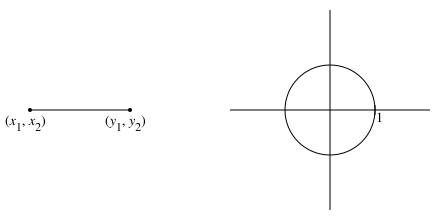
\includegraphics[width=\linewidth]{external/Euclidean_metric.pdf}
\end{image}%
\tcblower
\end{figureptx}%
Using this metric, the distance between two points \((x_1,x_2)\) and \((y_1,y_2)\) is the length of the segment connecting the points, while the unit circle (the set of points a distance 1 from the origin) looks like what we think of as a circle as illustrated in \hyperref[figure-F_Euclidean_metric]{Figure~{\xreffont\ref{figure-F_Euclidean_metric}}}.%
\par
As we will see, there are many other metrics that can be defined on \(\R^n\), or on other sets.%
\begin{exploration}{Preview Activity}{}{exploration-sec_metric_space_intro-g}%
\index{metric!taxicab}%
Consider the function \(d_T\) that assigns to each pair of points in \(\R^2\) the real number%
\begin{equation*}
d_T((x_1,x_2),(y_1,y_2)) = | x_1-y_1 | + | x_2-y_2 |\text{.}
\end{equation*}
%
\par
This function \(d_T\) is sometimes called the \terminology{taxicab metric} or \terminology{distance} because the distance between points \(x\) and \(y\) can be thought of as obtained by driving around a city block rather than going directly from point \(x\) to point \(y\).%
\par
Any distance function should satisfy certain properties: the distance between two points should never be negative, the distance from point \(A\) to point \(B\) should be the same as the distance from point \(B\) to point \(A\), the shortest distance between two points \(A\) and \(B\) should never be more than the distance from \(A\) to some point \(C\) plus the distance from \(C\) to \(B\), and the distance between points should only be zero if the points are the same. In this activity, we determine if \(d_T\) has these properties. Let \(x=(x_1,x_2)\) and \(y=(y_1,y_2)\) in \(\R^2\).%
\begin{enumerate}[font=\bfseries,label=(\alph*),ref=\alph*]%
\item{}Prove that \(d_T(x,y) \geq 0\).%
\item{}Prove that \(d_T(x,y) = d_T(y,x)\).%
\item{}Prove that \(d_T(x,y) = 0\) if and only if \(x = y\).%
\item{}Let \(z = (z_1,z_2)\) in \(\R^2\). Read the proof of \hyperref[lemma-lem_abs_TI]{Lemma~{\xreffont\ref{lemma-lem_abs_TI}}} (below) and then use \hyperref[lemma-lem_abs_TI]{Lemma~{\xreffont\ref{lemma-lem_abs_TI}}} to show that%
\begin{equation*}
d_T(x,y) \leq d_T(x,z) + d_T(z,y)\text{.}
\end{equation*}
%
\par
(Do you have any questions about the proof of the lemma?)%
\begin{lemma}{Lemma}{}{}{lemma-lem_abs_TI}%
Let \(a\) and \(b\) be real numbers. Then%
\begin{equation*}
| a+b | \leq | a | + | b |\text{.}
\end{equation*}
%
\end{lemma}
\begin{proof}{Proof}{}{proof-lem_abs_TI-b}
Let \(a\) and \(b\) be real numbers. To prove the lemma we consider cases.%
\begin{descriptionlist}
\begin{dlinarrow}{Case 1: \(a \geq 0\) and \(b \geq 0\)}{li-lem_abs_TI-b-a-c-a}%
In this case \(a+b\) is nonnegative and so \(| a | = a\), \(| b | = b\), and \(| a+b | = a+b\). Then%
\begin{equation*}
| a+b | = a+b =  | a | + | b |\text{.}
\end{equation*}
%
\end{dlinarrow}%
\begin{dlinarrow}{Case 2: \(a \leq 0\) and \(b \leq 0\)}{li-lem_abs_TI-b-a-c-b}%
In this case \(a = -a'\) and \(b = -b'\) where \(a'\) and \(b'\) are nonnegative. It follows from Case 1 that%
\begin{align*}
| a+b | \amp = | -(a'+b') | = | a'+b' | = a'+b' = | a' | + | b' |\\
\amp = | -a' | + | -b' | = | a | + | b |\text{.}
\end{align*}
%
\end{dlinarrow}%
\begin{dlinarrow}{Case 3: One of \(a\) or \(b\) is positive and the other negative}{li-lem_abs_TI-b-a-c-c}%
Without loss of generality we assume \(a \gt 0\) and \(b \lt 0\). Again we consider cases. Note that \(b \lt 0\) implies \(a+b \lt a\).%
\begin{itemize}[label=\textbullet]
\item{}Suppose \(b \geq -2a\). Then \(a+b \geq -a\) and so \(-a \leq a+b \lt  a\). It follows that%
\begin{equation*}
| a+b | \leq a = | a | \lt  | a | + | b |\text{.}
\end{equation*}
%
\item{}The last case is when \(b \lt  -2a\). In this case \(-b \gt 2a\) and so%
\begin{equation*}
| b | = -b \gt 2a = 2| a | \gt | a |\text{.}
\end{equation*}
Then \(a+b \lt  a = | a | \lt  | b |\). Finally, \(a \gt 0\) implies \(a+b \gt b = -| b |\). So%
\begin{equation*}
- | b | \lt  a+b \lt  | b |
\end{equation*}
and%
\begin{equation*}
| a+b | \leq | b | \lt  | a | + | b |\text{.}
\end{equation*}
%
\end{itemize}
%
\end{dlinarrow}%
\end{descriptionlist}
This proves our lemma for every possible pair \(a\), \(b\).%
\end{proof}
\item{}A picture to illustrate the taxicab distance \(d_T\) between (points \(x_1,x_2)\) and \((y_1,y_2)\) is shown in \hyperref[figure-F_PA_metric]{Figure~{\xreffont\ref{figure-F_PA_metric}}}. Draw a picture of the unit circle (the set of points a distance 1 from the origin) using the Taxicab metric. Explain your reasoning.%
\begin{figureptx}{Figure}{The taxicab distance between \((x_1,x_2)\) and \((y_1,y_2)\) in \(\R^2\).}{figure-F_PA_metric}{}%
\begin{image}{0.25}{0.5}{0.25}{}%
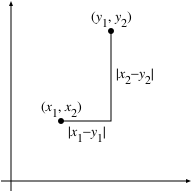
\includegraphics[width=\linewidth]{external/Taxicab.pdf}
\end{image}%
\tcblower
\end{figureptx}%
\end{enumerate}%
\end{exploration}%
The taxicab metric can be extended to \(\R^n\) for any \(n \geq 1\) as follows. If \(x = (x_1, x_2, \ldots,
x_n)\) and \(y = (y_1, y_2, \ldots,
y_n)\) are in \(\R^n\), then the taxicab distance \(d_T(x,y)\) from \(x\) to \(y\) is defined as%
\begin{equation*}
d_T(x,y) = |x_1-y_1| + |x_2-y_2| + \cdots + |x_n-y_n| = \sum_{i=1}^n |x_i-y_i|\text{.}
\end{equation*}
%
\end{sectionptx}
%
%
\typeout{************************************************}
\typeout{Section  Metric Spaces}
\typeout{************************************************}
%
\begin{sectionptx}{Section}{Metric Spaces}{}{Metric Spaces}{}{}{section-sec_metric_space}
For most of our mathematical careers our mathematics has taken place in \(\R^2\), where we measure the distance between points \((x_1,x_2)\) and \((y_1,y_2)\) with the standard Euclidean distance \(d_E\). In our preview activity we saw that the function \(d_T\) satisfies many of the same properties as \(d_E\). These properties allow us to use \(d_E\) or \(d_T\) as distance functions. We call any distance function a \terminology{metric}, and any space on which a metric is defined is called a \terminology{metric space}.%
\begin{definition}{Definition}{}{definition-sec_metric_space-c}%
\index{metric}%
A \terminology{metric} on a space \(X\) is a function \(d : X \times X \to \R^+ \cup \{0\}\) that satisfies the properties:%
\begin{enumerate}
\item{}\(d(x,y) \geq 0\) for all \(x,y \in X\),%
\item{}\(d(x,y) = 0\) if and only if \(x = y\) in \(X\),%
\item{}\(d(x,y) = d(y,x)\) for all \(x, y \in X\), and%
\item{}\(d(x,y) \leq d(x,z) + d(z,y)\) for all \(x,y,z \in X\).%
\end{enumerate}
%
\end{definition}
Properties 1 and 2 of a metric say that a metric is \terminology{positive definite}, while property 3 states that a metric is \terminology{symmetric}. Property 4 of the definition is usually the most difficult property to verify for a metric and is called the \terminology{triangle inequality}. \index{triangle inequality}%
\begin{definition}{Definition}{}{definition-sec_metric_space-e}%
\index{metric space}%
A \terminology{metric space} is a pair \((X,d)\), where \(d\) is a metric on the space \(X\).%
\end{definition}
When the metric is clear from the context, we just refer to \(X\) as the metric space.%
\begin{activity}{Activity}{}{activity-act_MS_metrics}%
For each of the following, determine if \((X,d)\) is a metric space. If \((X,d)\) is a metric space, explain why. If \((X,d)\) is not a metric space, determine which properties of a metric \(d\) satisfies and which it does not. If \((X,d)\) is a metric space, give a geometric description of the unit circle (the set of all points in \(X\) a distance \(1\) from the zero element) in the space.%
\begin{enumerate}[font=\bfseries,label=(\alph*),ref=\alph*]%
\item{}\(X = \R\), \(d(x,y) = \max\{|x|,|y|\}\).%
\item{}\(X = \R\), \(d(x,y) = \begin{cases}0 \amp \text{ if } x=y \\ 1 \amp \text{ if } x \neq y. \end{cases}\)%
\item{}\(X = \R^2\), \(d((x_1,x_2),(y_1,y_2)) = \max\{| x_1-y_1 |, | x_2-y_2 | \}\)%
\item{}\(X = C[0,1]\), the set of all continuous functions on the interval \([0,1]\),%
\begin{equation*}
d(f,g) = \ds \int_0^1 | f(x) - g(x) | \, dx\text{.}
\end{equation*}
%
\end{enumerate}%
\end{activity}%
It should be noted that not all metric spaces are infinite. We discuss one metric on a finite space in the following example.%
\begin{example}{Example}{}{example-exp_finite_ms}%
Let \(X = \{a,b,c\}\) and define \(d: A \times A \to \R^+ \cup \{0\}\) with the entries in \hyperref[table-T_finite_metric_ex]{Table~{\xreffont\ref{table-T_finite_metric_ex}}}.%
\begin{tableptx}{Table}{\textbf{Table of values for a function \(d\)}}{table-T_finite_metric_ex}{}%
\centering%
{\tabularfont%
\begin{tabular}{llll}
\multicolumn{1}{lA}{{\bfseries{}}}&\(a\)&\(b\)&\(c\)\tabularnewline\hrulethin
\multicolumn{1}{lA}{{\bfseries{}\(a\)}}&\(0\)&\(3\)&\(5\)\tabularnewline[0pt]
\multicolumn{1}{lA}{{\bfseries{}\(b\)}}&\(3\)&\(0\)&\(4\)\tabularnewline[0pt]
\multicolumn{1}{lA}{{\bfseries{}\(c\)}}&\(5\)&\(4\)&\(0\)
\end{tabular}
}%
\end{tableptx}%
By definition we have \(d(x,y) \geq 0\) for all \(x,
y \in X\) with \(d(x,y) = 0\) if and only if \(x=y\). Since the table is symmetric around the diagonal, we can see that \(d(x,y) = d(y,x)\) for all \(x,y \in X\). The only item to verify is the triangle inequality. If \(d(x,y) = 0\), then%
\begin{equation*}
d(x,y) = 0 \leq d(x,z) + d(z,y)
\end{equation*}
for any \(x,y \in X\). If \(d(x,z) = 0\), then \(x=z\) and%
\begin{equation*}
d(x,y) = d(z,y) \leq d(z,z) + d(z,y)\text{.}
\end{equation*}
%
\par
That leaves three cases to consider, when \(x\), \(y\), and \(z\) are distinct. Now%
\begin{align*}
d(a,b) \amp = 3 \leq 5+4 = d(a,c) + d(c,b),\\
d(a,c) \amp = 5 \leq 3+4 = d(a,b) + d(b,c),\\
d(b,c) \amp = 4 \leq 3+5 = d(b,a) + d(a,c)\text{.}
\end{align*}
%
\par
So \(d\) is a metric on \(X\).%
\end{example}
\hyperref[example-exp_finite_ms]{Example~{\xreffont\ref{example-exp_finite_ms}}} shows that even finite sets can be metric spaces. In fact, we can make a finite metric space by taking any finite subset \(S\) of a metric space \((X,d)\) and use as a metric the restriction of \(d\) to \(S\). \hyperref[example-exp_finite_ms]{Example~{\xreffont\ref{example-exp_finite_ms}}} illustrates this by letting \(a = (0,0)\), \(b = (3,0)\), and \(c = (3,4)\) in \(\R^2\). Then \(d\) is the restriction of the Euclidean metric to the set \(X\). Another way to construct a finite metric space is to start with a finite set of points and make a graph with the points as vertices. Construct edges so that the graph is connected (that is, there is a path from any one vertex to any other) and give weights to the edges as illustrated in \hyperref[figure-F_Graph_metric]{Figure~{\xreffont\ref{figure-F_Graph_metric}}}. We then define a metric \(d\) on \(S\) by letting \(d(x,y)\) be the length of a shortest path between vertices \(x\) and \(y\) in the graph. For example, \(d(b,c) = d(b,e) + d(e,c) = 9\) in this example.%
\begin{figureptx}{Figure}{A graph to define a metric.}{figure-F_Graph_metric}{}%
\begin{image}{0.35}{0.3}{0.35}{}%
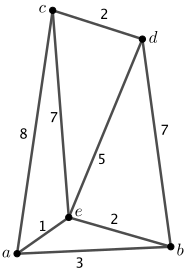
\includegraphics[width=\linewidth]{external/Graph_metric.pdf}
\end{image}%
\tcblower
\end{figureptx}%
Just as with the Euclidean and taxicab metrics, item (c) in \hyperref[activity-act_MS_metrics]{Activity~{\xreffont\ref{activity-act_MS_metrics}}} can be extended to \(\R^n\) as follows. If \(x = (x_1, x_2, \ldots,
x_n)\) and \(y = (y_1, y_2, \ldots,
y_n)\) are in \(\R^n\), then the maximum distance \(d_M(x,y)\) from \(x\) to \(y\) is defined as%
\begin{equation*}
d_M(x,y) = \max\{| x_1-y_1 |, | x_2-y_2 |, |x_3-y_3|, \ldots, |x_n-y_n| \} = \max_{1 \leq i \leq n} \{|x_i-y_i|\}\text{.}
\end{equation*}
%
\par
\index{metric!max} The metric \(d_M\) is called the \terminology{max} metric. In the following section we prove that the Euclidean metric is in fact a metric. Proofs that \(d_T\) and \(d_M\) are metrics are left to \hyperlink{exercise-ex_Taxicab}{Exercise~{\xreffont 5}} and \hyperlink{exercise-ex_Max}{Exercise~{\xreffont 6}}.%
\end{sectionptx}
%
%
\typeout{************************************************}
\typeout{Section  The Euclidean Metric on \(\R^n\)}
\typeout{************************************************}
%
\begin{sectionptx}{Section}{The Euclidean Metric on \(\R^n\)}{}{The Euclidean Metric on \(\R^n\)}{}{}{section-sec_euclid_rn}
The metric space that is most familiar to us is the metric space \((\R^2, d_E)\), where%
\begin{equation*}
d_E((x_1,x_2), (y_1,y_2)) = \sqrt{(x_1-y_1)^2 + (x_2-y_2)^2}
\end{equation*}
%
\par
\index{metric!Euclidean} The metric \(d_E\) called the \terminology{standard} or \terminology{Euclidean} metric on \(\R^2\).%
\par
We can generalize this Euclidean metric from \(\R^2\) to any dimensional real space. Let \(n\) be a positive integer and let \(x = (x_1, x_2, \ldots,
x_n)\) and \(y = (y_1, y_2, \ldots,
y_n)\) be in \(\R^n\). We define \(d_E : \R^n \times \R^n \to \R\) by%
\begin{equation*}
d_E(x,y) = \sqrt{(x_1-y_1)^2 + (x_2-y_2)^2 + \cdots (x_n-y_n)^2} = \sqrt{\sum_{i=1}^n (x_i-y_i)^2}\text{.}
\end{equation*}
%
\par
In the next activity we will show that \(d_E\) satisfies the first three properties of a metric.%
\begin{activity}{Activity}{}{activity-sec_euclid_rn-f}%
Let \(x = (x_1, x_2, \ldots,
x_n)\) and \(y = (y_1, y_2, \ldots,
y_n)\) be in \(\R^n\).%
\begin{enumerate}[font=\bfseries,label=(\alph*),ref=\alph*]%
\item{}Show that \(d_E(x,y) \geq 0\).%
\item{}Show that \(d_E(x,y) = d_E(y,x)\).%
\item{}Show that if \(x=y\), then \(d_E(x,y) = 0\).%
\item{}Show that if \(d_E(x,y) = 0\), then \(x=y\).%
\end{enumerate}%
\end{activity}%
Proving that the triangle inequality is satisfied is often the most difficult part of proving that a function is a metric. We will work through this proof with the help of the Cauchy-Schwarz Inequality.%
\begin{lemma}{Lemma}{Cauchy-Schwarz Inequality.}{}{lemma-lem_CS_Euclidean}%
\index{Cauchy-Schwarz Inequality}%
Let \(n\) be a positive integer and \(x = (x_1, x_2, \ldots,
x_n)\), \(y=(y_1, y_2, \ldots, y_n)\) be in \(\R^n\). Then%
\begin{equation}
\sum_{i=1}^n x_iy_i \leq  \left(\sqrt{\sum_{i=1}^n x_i^2}\right) \left(\sqrt{\sum_{i=1}^n y_i^2}\right)\text{.}\label{men-eq_SL}
\end{equation}
%
\end{lemma}
\begin{activity}{Activity}{}{activity-sec_euclid_rn-i}%
Before we prove the Cauchy-Schwarz Inequality, let us analyze it in two specific situations.%
\begin{enumerate}[font=\bfseries,label=(\alph*),ref=\alph*]%
\item{}Let \(x=(1,4)\) and \(y = (3,2)\) in \(\R^2\). Verify the Cauchy-Schwarz Inequality in this case.%
\item{}Let \(x=(1,2, -3)\) and \(y = (-4, 0, -1)\) in \(\R^3\). Verify the Cauchy-Schwarz Inequality in this case.%
\end{enumerate}%
\end{activity}%
Now we prove the Cauchy-Schwarz Inequality.%
\begin{proof}{Proof}{}{proof-sec_euclid_rn-k}
Let \(n\) be a positive integer and \(x = (x_1, x_2, \ldots,
x_n)\), \(y=(y_1, y_2, \ldots, y_n)\) be in \(\R^n\). To verify \hyperref[men-eq_SL]{({\xreffont\ref{men-eq_SL}})} it suffices to show that%
\begin{equation*}
\left(\sum_{i=1}^n x_iy_i\right)^2 \leq  \left(\sum_{i=1}^n x_i^2\right) \left(\sum_{i=1}^n y_i^2\right)\text{.}
\end{equation*}
%
\par
This is difficult to do directly, but there is a nice trick one can use. Consider the expression%
\begin{equation*}
\sum (x_i-\lambda y_i)^2\text{.}
\end{equation*}
%
\par
(All of our sums are understood to be from 1 to \(n\), so we will omit the limits on the sums for the remainder of the proof.) Now%
\begin{align}
0 \amp  \leq \sum (x_i-\lambda y_i)^2\notag\\
\amp = \sum \left(x_i^2 - 2\lambda x_iy_i + \lambda^2 y_i^2 \right)\notag\\
\amp = \left( \sum y_i^2 \right)\lambda^2 - 2\left(\sum x_iy_i\right) \lambda + \left(\sum x_i^2\right)\text{.}\label{mrow-eq_SL_1}
\end{align}
%
\par
To interpret this last expression more clearly, let \(a=\sum y_i^2\), \(b=-2\sum x_iy_i\) and \(c = \sum x_i^2\). The inequality defined by \hyperref[mrow-eq_SL_1]{({\xreffont\ref{mrow-eq_SL_1}})} can then be written in the form%
\begin{equation*}
p(\lambda) = a \lambda^2 + b \lambda + c \geq 0\text{.}
\end{equation*}
%
\par
So we have a quadratic \(p(\lambda)\) that is never negative. This implies that the quadratic \(p(\lambda)\) can have at most one real zero. The quadratic formula gives the roots of \(p(\lambda)\) as%
\begin{equation*}
\frac{-b \pm \sqrt{b^2-4ac}}{2a}\text{.}
\end{equation*}
%
\par
If \(b^2-4ac \gt 0\), then \(p(\lambda)\) has two real roots. Therefore, in order for \(p(\lambda)\) to have at most one real zero we must have%
\begin{equation*}
0 \geq b^2-4ac = 4 \left(\sum x_iy_i\right)^2 - 4\left(\sum y_i^2\right)\left(\sum x_i^2\right)
\end{equation*}
or%
\begin{equation*}
\left(\sum y_i^2\right)\left(\sum x_i^2\right) \geq \left(\sum x_iy_i\right)^2\text{.}
\end{equation*}
%
\par
This establishes the Cauchy-Schwarz Inequality.%
\end{proof}
One consequence of the Cauchy-Schwarz Inequality that we will need to show that \(d_E\) is a metric is the following.%
\begin{corollary}{Corollary}{}{}{corollary-cor_SL}%
Let \(n\) be a positive integer and \(x = (x_1, x_2, \ldots,
x_n)\), \(y=(y_1, y_2, \ldots, y_n)\) be in \(\R^n\). Then%
\begin{equation*}
\sqrt{\sum_{i=1}^n (x_i+y_i)^2} \leq \sqrt{\sum_{i=1}^n x_i^2} + \sqrt{\sum_{i=1}^n y_i^2}\text{.}
\end{equation*}
%
\end{corollary}
\begin{activity}{Activity}{}{activity-sec_euclid_rn-n}%
Before we prove the corollary, let us analyze it in two specific situations.%
\begin{enumerate}[font=\bfseries,label=(\alph*),ref=\alph*]%
\item{}Let \(x=(1,4)\) and \(y = (3,2)\) in \(\R^2\). Verify \hyperref[corollary-cor_SL]{Corollary~{\xreffont\ref{corollary-cor_SL}}} in this case.%
\item{}Let \(x=(1,2, -3)\) and \(y = (-4, 0, -1)\) in \(\R^3\). Verify \hyperref[corollary-cor_SL]{Corollary~{\xreffont\ref{corollary-cor_SL}}} in this case.%
\end{enumerate}%
\end{activity}%
Now we prove \hyperref[corollary-cor_SL]{Corollary~{\xreffont\ref{corollary-cor_SL}}}.%
\begin{proof}{Proof}{}{proof-sec_euclid_rn-p}
Let \(n\) be a positive integer and \(x = (x_1, x_2, \ldots,
x_n)\), \(y=(y_1, y_2, \ldots, y_n)\) be in \(\R^n\). Now%
\begin{align*}
\sum \left(x_i+y_i\right)^2 \amp = \sum \left(x_i^2 +2x_iy_i + y_i^2 \right)\\
\amp = \sum x_i^2 + 2\sum x_iy_i + \sum y_i^2\\
\amp \leq \sum x_i^2 + 2\left(\sqrt{\sum x_i^2}\right) \left(\sqrt{\sum y_i^2} \right) + \sum y_i^2\\
\amp = \left(\sqrt{\sum x_i^2} + \sqrt{\sum y_i^2}\right)^2\text{.}
\end{align*}
%
\par
Taking the square roots of both sides yields the desired inequality.%
\end{proof}
We can now complete the proof that \(d_E\) is a metric.%
\begin{activity}{Activity}{}{activity-sec_euclid_rn-r}%
Let \(n\) be a positive integer and \(x = (x_1, x_2, \ldots,
x_n)\), \(y=(y_1, y_2, \ldots, y_n)\), and \(z=(z_1, z_2, \ldots, z_n)\) be in \(\R^n\). Use \hyperref[corollary-cor_SL]{Corollary~{\xreffont\ref{corollary-cor_SL}}} to show that%
\begin{equation*}
d_E(x,y) \leq d_E(x,z)+d_E(z,y)\text{.}
\end{equation*}
%
\end{activity}%
This concludes our proof that the Euclidean metric is in fact a metric.%
\par
We have seen several metrics in this section, some of which are given special names. Let \(x = (x_1, x_2, \ldots,
x_n)\) and \(y = (y_1, y_2, \ldots, y_n)\)%
\begin{itemize}[label=\textbullet]
\item{}The Euclidean metric \(d_E\), where%
\begin{align*}
d_E(x,y) \amp = \sqrt{(x_1-y_1)^2 + (x_2-y_2)^2 + \cdots (x_n-y_n)^2}\\
\amp = \sqrt{\sum_{i=1}^n (x_i-y_i)^2}\text{.}
\end{align*}
%
\item{}The Taxicab metric \(d_T\), where%
\begin{equation*}
d_T(x,y) = |x_1-y_1| + |x_2-y_2| + \cdots + |x_n-y_n| = \sum_{i=1}^n \{|x_i-y_i|\}\text{.}
\end{equation*}
%
\item{}The max metric \(d_M\), where%
\begin{align*}
d_M(x,y) \amp = \max\{| x_1-y_1 |, | x_2-y_2 |, |x_3-y_3|, \ldots, |x_n-y_n| \}\\
\amp = \max_{1 \leq i \leq n} \{|x_i-y_i|\}\text{.}
\end{align*}
%
\end{itemize}
%
\par
We have only shown that \(d_T\) and \(d_M\) are metrics on \(\R^2\), but similar arguments apply in \(\R^n\). Proofs are left to \hyperlink{exercise-ex_Taxicab}{Exercise~{\xreffont 5}} and \hyperlink{exercise-ex_Max}{Exercise~{\xreffont 6}}. In addition, the \terminology{discrete metric} \index{metric!discrete}%
\begin{equation*}
d(x,y) = \begin{cases}0 \amp  \text{ if }  x=y \\ 1 \amp  \text{ if }  x \neq y \end{cases}
\end{equation*}
makes any set \(X\) into a metric space. The proof is left to \hyperlink{exercise-ex_MS_discrete}{Exercise~{\xreffont 1}}.%
\end{sectionptx}
%
%
\typeout{************************************************}
\typeout{Section  Summary}
\typeout{************************************************}
%
\begin{sectionptx}{Section}{Summary}{}{Summary}{}{}{section-sec_metric_space_summ}
Important ideas that we discussed in this section include the following.%
\begin{itemize}[label=\textbullet]
\item{}A metric on a space \(X\) is a function that measures distance between elements in the space. More formally, a metric on a space \(X\) is a function \(d: X \times X \to \R^+ \cup \{0\}\) such that%
\begin{enumerate}
\item{}\(d(x,y) \geq 0\) for all \(x,y \in X\),%
\item{}\(d(x,y) = 0\) if and only if \(x = y\) in \(X\),%
\item{}\(d(x,y) = d(y,x)\) for all \(x, y \in X\), and%
\item{}\(d(x,y) \leq d(x,z) + d(z,y)\) for all \(x,y,z \in X\).%
\end{enumerate}
A metric space is any space combined with a metric defined on that space.%
\item{}The Euclidean, taxicab, and max metric are all metrics on \(\R^n\), so they all provide ways to measure distances between points in \(\R^n\). These metric are different in how they define the distances.%
\begin{itemize}[label=$\circ$]
\item{}The Euclidean metric is the standard metric that we have used through our mathematical careers. For elements \(x = (x_1, x_2, \ldots,
x_n)\) and \(y = (y_1, y_2, \ldots,
y_n)\) in \(\R^n\), the Euclidean metric \(d_E\) is defined as%
\begin{align*}
d_E(x,y) \amp =  \sqrt{(x_1-y_1)^2 + (x_2-y_2)^2 + \cdots (x_n-y_n)^2}\\
\amp = \sqrt{\sum_{i=1}^n (x_i-y_i)^2}\text{.}
\end{align*}
With this metric, the unit circle in \(\R^2\) (the set of points a distance \(1\) from the origin) is the standard unit circle we know from Euclidean geometry.%
\item{}The taxicab metric \(d_T\) is defined as%
\begin{align*}
d_T(x,y) \amp = |x_1-y_1| + |x_2-y_2| + \cdots + |x_n-y_n|\\
\amp = \sum_{i=1}^n |x_i-y_i|\text{.}
\end{align*}
The unit circle in \(\R^2\) using the taxicab metric is the square with vertices \((1,0)\), \((0,1)\), \((-1,0)\), and \((0,-1)\) when viewed in Euclidean geometry.%
\item{}The max metric \(d_M\) is defined by%
\begin{align*}
d_M(x,y) \amp = \max\{| x_1-y_1 |, | x_2-y_2 |, |x_3-y_3|, \ldots, |x_n-y_n| \}\\
\amp = \max_{1 \leq i \leq n} \{|x_i-y_i|\}\text{.}
\end{align*}
Under the max metric, the unit circle in \(\R^2\) is the square with vertices \((1,1)\), \((-1,1)\), \((-1,-1)\), and \((1,-1)\) when viewed in Euclidean geometry.%
\end{itemize}
%
\end{itemize}
%
\end{sectionptx}
%
%
\typeout{************************************************}
\typeout{Exercises  Exercises}
\typeout{************************************************}
%
\begin{exercises-section}{Exercises}{Exercises}{}{Exercises}{}{}{exercises-sec_metric_space_exer}
\begin{divisionexercise}{1}{}{}{exercise-ex_MS_discrete}%
Let \(X\) be a set. Show that the function \(d\) (the discrete metric) defined by%
\begin{equation*}
d(x,y) = \begin{cases}0 \amp  \text{ if }  x=y \\ 1 \amp  \text{ if }  x \neq y \end{cases}
\end{equation*}
is a metric.%
\end{divisionexercise}%
\begin{divisionexercise}{2}{}{}{exercise-ex_MS_mod_metric}%
Let \(X = \{1,3,5\} \subset \Z\) and define \(d: X \times X \to \R\) by \(d(x,y) = xy - 1 \pmod{n}\). That is, \(d(x,y)\) is the remainder when \(xy - 1\) is divided by \(n\).%
\begin{itemize}[label=\textbullet]
\item{}For each value of \(n\), determine if \(d\) defines a metric on \(X\). Prove your answers.%
\item{}The unit circle in \(\R^2\) with metric \(d\) is the set of all points in \(\R^2\) whose distance from the origin is \(1\). If we let the distance be less than \(1\), then we have what we call an open ball. We can make this same definition in any metric space. \begin{definition}{Definition}{}{definition-def_ms_open_ball}%
\index{open ball in a metric space}Let \((Y, d_Y)\) be a metric space. For any positive real number \(r\), the \terminology{open ball centered at \(b\) of radius} \(r\) in \((Y, d_Y)\) is the the set%
\begin{equation*}
B(b,r) = \{y \in Y \mid d_Y(y,b) \lt  r\}\text{.}
\end{equation*}
%
\end{definition}
 If \((X,d)\) is a metric space for a given value of \(n\), determine all of the open balls in \(X\) centered at \(1\). If \((X,d)\) is not a metric space, explain why.%
\end{itemize}
%
\begin{enumerate}[font=\bfseries,label=(\alph*),ref=\alph*]%
\item{}\(n = 4\)%
\item{}\(n = 8\)%
\end{enumerate}%
\end{divisionexercise}%
\begin{divisionexercise}{3}{}{}{exercise-ex_MS_Q_metric}%
Let \(Q\) be the set of all rational numbers in reduced form. A rational number \(\frac{r}{s}\) is in reduced form if \(s \gt 0\) and \(r\) and \(s\) have no common factors larger than \(1\). Define \(d : Q \times Q \to \R\) by%
\begin{equation*}
d\left(\frac{a}{b}, \frac{r}{s}\right) = \max\{| a-r |, | b-s |\}\text{.}
\end{equation*}
%
\begin{enumerate}[font=\bfseries,label=(\alph*),ref=\alph*]%
\item{}Prove that \(d\) is a metric.%
\item{}A metric allows us to determine which elements in our metric space are '{}'{}close'{}'{} together. Describe the set of elements in \(Q\) that are a distance no more than \(1\) from \(\frac{2}{3}\) using this metric \(d\). In other words, describe the open ball centered at \(\frac{2}{3}\) with radius \(1\) (see \hyperref[definition-def_ms_open_ball]{Definition~{\xreffont\ref{definition-def_ms_open_ball}}}).%
\item{}If \(a\), \(b\), and \(c\) are elements of a metric space \((X, d_X)\), we say that \(b\) is between \(a\) and \(c\) if \(d_X(a,c) = d_X(a,b) + d_X(b,c)\). Using the Euclidean metric on \(\Q\), there are infinitely many different rational numbers between \(0\) and \(1\) (the rational numbers between \(0\) and \(1\) that lie on the Euclidean line through \(0\) and \(1\). Describe all of the points in \((\Q,d)\) that are between \(0\) and \(1\).%
\end{enumerate}%
\end{divisionexercise}%
\begin{divisionexercise}{4}{}{}{exercise-sec_metric_space_exer-d}%
Let \((\Q,d)\) be the metric space from \hyperlink{exercise-ex_MS_Q_metric}{Exercise~{\xreffont 3}}. If \(a\), \(b\), and \(c\) are elements of a metric space \((X, d_X)\), we say that \(b\) is \terminology{between} \(a\) and \(c\) if \(d_X(a,c) = d_X(a,b) + d_X(b,c)\). Using the Euclidean metric on \(\Q\), there are infinitely many different rational numbers between \(0\) and \(1\) (the rational numbers between \(0\) and \(1\) that lie on the Euclidean line through \(0\) and \(1\). In this exercise we explore numbers that are between others in the space \((\Q,d)\).%
\begin{enumerate}[font=\bfseries,label=(\alph*),ref=\alph*]%
\item{}Find all of the elements in \((\Q,d)\) that are between \(0\) and \(1\).%
\item{}Which is closer to \(0\) in \((\Q,d)\): \(1\) or \(\frac{1}{3}\)?%
\item{}Now find all of the elements in \((\Q,d)\) that are between \(0\) and \(\frac{1}{3}\).%
\end{enumerate}%
\end{divisionexercise}%
\begin{divisionexercise}{5}{}{}{exercise-ex_Taxicab}%
Prove that the taxicab metric \(d_T\) is a metric on \(\R^n\).%
\end{divisionexercise}%
\begin{divisionexercise}{6}{}{}{exercise-ex_Max}%
Let \(A\) and \(B\) be nonempty finite subsets of \(\R^n\), and let \(A+B = \{a+b \mid a \in A, b \in B\}\).%
\begin{enumerate}[font=\bfseries,label=(\alph*),ref=\alph*]%
\item{}Prove that \(\max (A+B) \leq \max A + \max B\).%
\item{}Prove that the max metric \(d_M\) is a metric on \(\R^n\).%
\end{enumerate}%
\end{divisionexercise}%
\begin{divisionexercise}{7}{}{}{exercise-ex_MS_hub}%
If \(x = (x_1, x_2, \ldots, x_n)\), we let \(|x| = \sqrt{x_1^2+x_2^2+ \cdots + x_n^2}\). For \(x = (x_1, x_2, \ldots,
x_n)\) and \(y = (y_1, y_2, \ldots y_n)\), define \(d_H: \R^n \times \R^n \to \R\) by%
\begin{equation*}
d_H(x,y) = \begin{cases}0 \amp \text{ if }  x=y \\ |x|+|y| \amp \text{ otherwise } . \end{cases}
\end{equation*}
%
\begin{enumerate}[font=\bfseries,label=(\alph*),ref=\alph*]%
\item{}Show that \(d_H\) is a metric (called the \terminology{hub} metric).%
\item{}\begin{enumerate}[font=\bfseries,label=(\roman*),ref=\theenumi.\roman*]%
\item{}Let \(a = \left(\frac{1}{2}, 0\right)\). Explicitly describe which points are in the set \(B(a,1)\) in \((\R^2, d_H)\). (See \hyperlink{exercise-ex_MS_mod_metric}{Exercise~{\xreffont 2}} for the definition of an open ball.)%
\item{}Let \(a = (3,4)\). Explicitly describe which points are in the set \(B(a,1)\) in \((\R^2, d_H)\).%
\item{}Now explicitly describe all open balls in \((\R^2, d_H)\).%
\end{enumerate}%
\end{enumerate}%
\end{divisionexercise}%
\begin{divisionexercise}{8}{}{}{exercise-sec_metric_space_exer-h}%
Let \(\Z\) be the set of integers and let \(p\) be a prime. For each pair of distinct integers \(m\) and \(n\) there is an integer \(t = t(m,n)\) such that \(|m-n| = k \times p^t\), where \(p\) does not divide \(k\). For example, if \(p=5\), \(m = 34\), and \(n = 7\), then \(m-n = 27 = 27 \times 5^0\). So \(t(43,7) = 27\). However, if \(m = 54\) and \(n = 4\), then \(m-n = 50 = 2 \times 5^2\). So \(t(54,4) = 2\). Define \(d: \Z \times \Z \to \R\) by%
\begin{equation*}
d(m,n) = \begin{cases}0 \amp \text{ if }  m=n \\ \frac{1}{p^t} \amp \text{ if }  m \neq n. \end{cases}
\end{equation*}
%
\begin{enumerate}[font=\bfseries,label=(\alph*),ref=\alph*]%
\item{}Determine the values of \(d(62,170)\) using \(p=3\) and \(d(14008,2003)\) using \(p=7\).%
\item{}Prove that if \(a\), \(b\), and \(c\) are in \(\Z\), then%
\begin{equation*}
t(a,c) \geq \min\{t(a,b), t(b,c)\}\text{.}
\end{equation*}
%
\item{}Prove that \((\Z,d)\) is a metric space.%
\item{}Let \(p = 3\). Describe the set of all elements \(x\) in \((\Z,d)\) such that \(d(x,0) = 1\).%
\item{}Continue with \(p=3\). Describe the set of all elements \(x\) in \((\Z,d)\) such that \(d(x,0) \lt \frac{1}{2}\).%
\end{enumerate}%
\end{divisionexercise}%
\begin{divisionexercise}{9}{}{}{exercise-sec_metric_space_exer-i}%
Let \((X, d_X)\) and \((Y, d_Y)\) be metric spaces. We can make the Cartesian product \(X \times Y\) into a metric space by defining a metric \(d'\) on \(X \times Y\) as follows. If \((x_1, y_2)\) and \((x_2, y_2)\) are in \(X \times Y\), then%
\begin{equation*}
d'((x_1,y_1), (x_2, y_2)) = \max\{d_X(x_1,x_2), d_Y(y_1,y_2)\}\text{.}
\end{equation*}
You may assume without proof that \(d'\) is a metric on \(X \times Y\).%
\begin{enumerate}[font=\bfseries,label=(\alph*),ref=\alph*]%
\item{}Let \((X, d_X) = (\R^2, d_M)\) and \((Y, d_Y) = (\R^2, d_T)\). Let \(u = ((1,2), (1,-1))\) and \(v = ((0,5),(2,-2))\). What is%
\begin{equation*}
d'(u,v)?
\end{equation*}
Recall that%
\begin{equation*}
d_M((x_1,x_2),(y_1,y_2)) = \max\{ | x_1-y_1 |, | x_2-y_2 |\}
\end{equation*}
and%
\begin{equation*}
d_T((x_1,x_2),(y_1,y_2)) = | x_1-y_1 | + | x_2-y_2 |\text{.}
\end{equation*}
%
\item{}Let \((X, d_X) = (\R, d_E)\) and \((Y, d_Y) = (\R, d)\), where \(d\) is the discrete metric. Let%
\begin{equation*}
A=\{(x,y) \in \R \times \R \mid -1\leq x \leq 1 \text{ and }  -1 \leq y \leq 1\}
\end{equation*}
in \(X \times Y\). Let \(a = (0,1)\) in \(X \times Y\). Describe, geometrically, what the open ball \(B(a,1)\) looks like in the product space \(X \times Y\). Draw a picture of this open ball.%
\end{enumerate}%
\end{divisionexercise}%
\begin{divisionexercise}{10}{}{}{exercise-sec_metric_space_exer-j}%
Let \(X = \R^+\), the set of positive reals, and define \(d: X \times X \to \R\) by%
\begin{equation*}
d(x,y) = |\ln(y/x)|\text{.}
\end{equation*}
Is \(d\) is a metric on \(X\)? Prove your answer.%
\end{divisionexercise}%
\begin{divisionexercise}{11}{}{}{exercise-ex_1_over_1_plus_t_metric}%
Let \(d: \R \times \R \to \R\) be defined by%
\begin{equation*}
d(x,y) = \frac{|x-y|}{|x-y|+1}\text{.}
\end{equation*}
Show that \(d\) is a metric on \(\R\). (Hint: For the triangle inequality, note that \(d(x,y) = f(|x-y|)\) where \(f(t) = \frac{t}{t+1}\), and \(f\) is an increasing function.)%
\end{divisionexercise}%
\begin{divisionexercise}{12}{}{}{exercise-sec_metric_space_exer-l}%
Let \((X,d)\) be a metric space and \(k\) be a constant. Define \(kd: X \times X \to \R\) by%
\begin{equation*}
(kd)(x,y) = kd(x,y)\text{.}
\end{equation*}
Under what, if any, conditions is \(kd\) a metric on \(X\). Justify your answer.%
\end{divisionexercise}%
\begin{divisionexercise}{13}{}{}{exercise-sec_metric_space_exer-m}%
A real valued function \(f\) on an interval is \terminology{concave} if%
\begin{equation}
f((1-\alpha)x + \alpha y) \geq (1-\alpha)f(x) + \alpha f(y)\label{men-eq_concave}
\end{equation}
for all \(\alpha \in [0,1]\) and all \(x\) and \(y\) in the interval. Note that the expression \((1-\alpha)x + \alpha y\) is linear in \(\alpha\) and is equal to \(x\) when \(\alpha = 0\) and \(y\) when \(\alpha = 1\). So \((1-\alpha)x + \alpha y\) is a parameterization of the line segment joining \(x\) to \(y\). As \hyperref[figure-F_concave]{Figure~{\xreffont\ref{figure-F_concave}}} indicates, equation \hyperref[men-eq_concave]{({\xreffont\ref{men-eq_concave}})} implies that the graph of a concave function \(f\) on any interval \([x,y]\) lies above the secant line joining the points \((x,f(x))\) and \((y,f(y))\).%
\begin{figureptx}{Figure}{A concave function.}{figure-F_concave}{}%
\begin{image}{0.25}{0.5}{0.25}{}%
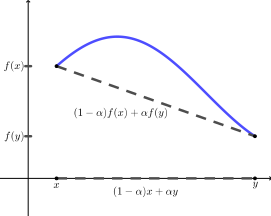
\includegraphics[width=\linewidth]{external/Concave.pdf}
\end{image}%
\tcblower
\end{figureptx}%
\begin{enumerate}[font=\bfseries,label=(\alph*),ref=\alph*]%
\item{}Let \(f(x) = -x^2\) map \(\R\) to \(\R\) with the standard Euclidean metric. Show that \(f\) is concave on the interval \([-1,1]\).%
\par\smallskip%
\noindent\textbf{\blocktitlefont Hint}.\hypertarget{hint-sec_metric_space_exer-m-b-b}{}\quad{}Start with the fact that \(\alpha(1-\alpha)(x-y)^2 \geq 0\).%
\item{}Show that if \(f\) is a concave function on \([0,\infty)\) and \(f(0) \geq 0\), an interval and \(a\) and \(b\) are in the interval, then%
\begin{equation*}
f(a) + f(b) \geq f(a+b)\text{.}
\end{equation*}
%
\par\smallskip%
\noindent\textbf{\blocktitlefont Hint}.\hypertarget{hint-sec_metric_space_exer-m-c-b}{}\quad{}Consider \hyperref[men-eq_concave]{({\xreffont\ref{men-eq_concave}})} with \(y=0\). Then use the fact that \(\frac{a}{a+b}\) is in \([0,1]\).%
\item{}Suppose \((X,d)\) is a metric space and \(f: [0, \infty) \to [0, \infty)\) is an increasing, concave function such that \(f(x) = 0\) if and only if \(x=0\). Prove that \(f \circ d\) is a metric on \(X\).%
\end{enumerate}%
\end{divisionexercise}%
\begin{divisionexercise}{14}{}{}{exercise-sec_metric_space_exer-n}%
For each of the following, answer true if the statement is always true. If the statement is only sometimes true or never true, answer false and provide a concrete example to illustrate that the statement is false. If a statement is true, explain why.%
\begin{enumerate}[font=\bfseries,label=(\alph*),ref=\alph*]%
\item{}The function \(d: \R \times \R \to \R\) defined by \(d(x,y) = (x-y)^2\) is a metric on \(\R\).%
\item{}Every nonempty set can be made into a metric space.%
\item{}It is possible to define an infinite number of metrics on every set containing at least two elements.%
\item{}Let \((X, d_X)\) and \((Y, d_Y)\) be metric spaces with \(|X| \geq 2\). Then the function \(d: X \times Y \to \R\) defined by \(d((a,b),(c,d)) = d_X(a,c)d_Y(b,d)\) is a metric on \(X \times Y\).%
\item{}Let \((X,d)\) be a metric space. If \(X\) is infinite, then the range of \(d\) is also an infinite set.%
\end{enumerate}%
\end{divisionexercise}%
\end{exercises-section}
\end{chapterptx}
 %
%
\typeout{************************************************}
\typeout{Chapter 4 Applications of Metric Spaces}
\typeout{************************************************}
%
\begin{chapterptx}{Chapter}{Applications of Metric Spaces}{}{Applications of Metric Spaces}{}{}{chapter-chap_metric_spaces_apps}
\renewcommand*{\chaptername}{Chapter}
%
%
\typeout{************************************************}
\typeout{Section  Introduction}
\typeout{************************************************}
%
\begin{sectionptx}{Section}{Introduction}{}{Introduction}{}{}{section-sec_met_space_app}
In this section we explore two applications of metric spaces.%
\end{sectionptx}
%
%
\typeout{************************************************}
\typeout{Section  The Hamming Metric}
\typeout{************************************************}
%
\begin{sectionptx}{Section}{The Hamming Metric}{}{The Hamming Metric}{}{}{section-sec_hamming}
In our society, a great deal of information is communicated electronically. Bank transactions, television programs, military communications, cell phone calls, digital images, and almost any interchange one can think of either can be or is digitized and transmitted electronically. In many situations we need to compare one set of data to another (e.g., Internet searches for text strings or image matches, DNA strands), and metrics are often used for this purpose. Computers work in a binary system, that is they recognize only zeros and ones. So a digital text message is a string of zeros and ones. That is, a digital message is a collection of elements in the space \(X^n\) for some positive integer \(n\), where \(X = \{0,1\}\). Each element in \(X^n\) is called a \terminology{word} - that is, a word is an element in \(X^n\) denoted in the form \((x_1, x_1, \ldots,
x_n)\). Just like in the English language, where not every combination of letters corresponds to words that make sense, not every word is recognizable as part of an intelligible message. We might, for example, code the letters of the alphabet by assigning numbers 1-26 to the letters, then make them elements of \(X^n\) by converting to binary. The collection of all intelligible words is called a \terminology{code}. So a code is just some subset of \(X^n\) that all parties agree are sensible words. The words in a code are called \terminology{code words}. To deal with problems that occur in transmitting digital messages, like scrambling (\terminology{encoding}) messages, unscrambling (\terminology{decoding}) messages, and detecting and correcting errors in messages, it is useful to have a way to measure distance between words. One way is to use the Hamming metric.%
\begin{definition}{Definition}{}{definition-sec_hamming-c}%
\index{metric!Hamming}%
Let \(x = (x_1, x_2, \ldots,
x_n)\) and \(y = (y_1, y_2, \ldots,
y_n)\) be words in \(X^n\). The \terminology{Hamming distance} \(d_H\) between \(x\) and \(y\) is%
\begin{equation*}
d_H(x,y) = \sum_{i=1}^n | x_i-y_i |\text{.}
\end{equation*}
%
\end{definition}
Recall that for each \(i\) both \(x_i\) and \(y_i\) are either 0 or 1. So%
\begin{equation*}
| x_i-y_i | = \begin{cases}0 \amp \text{ if }  x_i=y_i \\ 1 \amp \text{ if }  x_i \neq y_i. \end{cases}
\end{equation*}
%
\par
In other words, \(d_H(x,y)\) counts the number of components at which \(x\) and \(y\) are different.%
\begin{activity}{Activity}{}{activity-sec_hamming-f}%
\begin{enumerate}[font=\bfseries,label=(\alph*),ref=\alph*]%
\item{}Explain why \(d_H\) is a metric.%
\item{}Suppose we create a code%
\begin{equation*}
C = \{c_1,c_2,c_3,c_4,c_5,c_6,c_7,c_8\}
\end{equation*}
in \(X^6\), where%
\begin{align*}
c_1 \amp = (0,0,0,0,0,0) \amp c_2 \amp =( 0,0,0,0,1,1) \amp c_3 \amp = (0,0,0,1,0,1)\\
c_4 \amp = (0,0,1,0,0,1) \amp c_5 \amp = (0,0,0,1,1,0) \amp c_6 \amp = (0,0,1,0,1,0)\\
c_7 \amp = (0,0,1,1,0,0) \amp c_8 \amp = (0,0,1,1,1,1) \amp \amp 
\end{align*}
That is, the words \(c_1\), \(c_2\), \(c_3\), \(c_4\), \(c_5\), \(c_6\), \(c_7\), \(c_8\) are the only words that can comprise a message. Find \(d_H(c_2, c_8)\).%
\item{}Suppose we are on the receiving end of the message%
\begin{equation}
(0,0,0,1,1,1) \ (0,0,1,1,0,0) \ (1,0,0,0,0,0) \ (0,0,0,0,1,1) \ (0,0,1,0,0,1)\text{.}\label{men-eq_message}
\end{equation}
%
\begin{enumerate}[font=\bfseries,label=(\roman*),ref=\theenumi.\roman*]%
\item{}How do we know that an error has occurred in transmission of the message we received?%
\item{}To correct the errors in this received message, we replace the incorrect words with the code word(s) in \(C\) closest to them. Correct this message. (Note that there may be more than one possible substitution. Find all of the possibilities.)%
\end{enumerate}%
\end{enumerate}%
\end{activity}%
\end{sectionptx}
%
%
\typeout{************************************************}
\typeout{Section  The Levenshtein Metric}
\typeout{************************************************}
%
\begin{sectionptx}{Section}{The Levenshtein Metric}{}{The Levenshtein Metric}{}{}{section-sec_levenshtein}
The Levenshtein metric is one measure of distance that researchers use to understand DNA. DNA is composed of double chains of nucleotides, which wind together to form a double helix. The nucleotides come in four types: adenine (A), cytosine (C), guanine (G), and thymine (T). The nucleotides in the two chains of a DNA strand pair together, (A with T, and C with G), so the nucleotides in one chain determine the nucleotides in the other. Therefore, we can represent a DNA strand with a string of letters from the alphabet \(\{A, C, G, T\}\). One problem DNA researchers have is how to compare two strands of DNA, and the Levenshtein metric is one way that the distance between strands can be measured. Other metrics could be used, but the Levenshtein metric is appropriate to the task for several reasons. During evolution, changes in DNA sequences arise due to nucleotide substitution, or the insertion or deletion of nucleotides. These evolutionary changes can be modeled by the operations that determine the Levenshtein distance better than other metrics. In addition, the Levenshtein metric can be used to calculate distances between strings of different lengths. The Levenshtein metric also has applications in spell checkers, speech recognition, and automated plagiarism detection. To understand how the Levenshtein metric is calculated, consider the question of how far apart the words ``green'' and ``grease'' are.%
\par
To compare these words, we have to be able to change letters, and add or delete letters. If \(x = x_1x_2 \cdots x_n\) is a string of letters, we allow the following operations:%
\begin{descriptionlist}
\begin{dlimedium}{a deletion:}{li-sec_levenshtein-c-b-a}%
replace \(x\) with \(x_1 \cdots x_{i-1}x_{i+1} \cdots x_n\) for some \(i\),%
\end{dlimedium}%
\begin{dlimedium}{an insertion:}{li-sec_levenshtein-c-b-b}%
replace \(x\) with \(x_1 \cdots x_{i}yx_{i+1} \cdots x_n\), where \(y\) is an allowable letter and \(0 \leq i \leq n\),%
\end{dlimedium}%
\begin{dlimedium}{a substitution:}{li-sec_levenshtein-c-b-c}%
replace \(x\) with \(x_1 \cdots x_{i-1}yx_{i+1} \cdots x_n\), where \(y\) is an allowable letter and \(1 \leq i \leq n\).%
\end{dlimedium}%
\end{descriptionlist}
%
\begin{activity}{Activity}{}{activity-sec_levenshtein-d}%
\begin{enumerate}[font=\bfseries,label=(\alph*),ref=\alph*]%
\item{}Using the allowable operations, change the word ``green'' into the word ``grease''. Specifically identify each operation you use. (Note: the intermediate strings of letters do not have to form recognizable words.) How many operations did you use?%
\item{}If it took three operations to transform ``green'' into ``grease'', we could say that the distance between ``green'' and ``grease'' is at most 3. However, it may be possible to transform ``green'' into ``grease'' in fewer than 3 operations, which might change our opinion of the distance between these words. In general, to define the Levenshtein distance \(d_L\) between a sting \(x\) and a string \(y\), let \(m_d\) denote the number of deletions, \(m_i\) the number of insertions, and \(m_s\) the number of substitutions we use to get from \(x\) to \(y\). There may be many different combinations of \(m_d\), \(m_i\), and \(m_s\) that get us from \(x\) to \(y\), so we want the smallest number. \begin{definition}{Definition}{}{definition-sec_levenshtein-d-b-a-a-t}%
\index{metric!Levenshtein}The \terminology{Levenshtein distance} \(d_L(x,y)\) between strings \(x\) and \(y\) is%
\begin{equation*}
d_L(x,y) = \min\{m_d+m_i+m_s\}\text{.}
\end{equation*}
%
\end{definition}
 Prove that the Levenshtein distance function is really a metric on the set of all possible words (sensical or nonsensical).%
\item{}A spell checker corrects the misspelled word ``tupotagry''. Using the Levenshtein metric, which word would the spell checker use as the closest to ``tupotagry''? Why?%
\begin{equation*}
\text{"topography} \qquad \text{"topology"} \qquad \text{"tautology"}
\end{equation*}
%
\end{enumerate}%
\end{activity}%
\end{sectionptx}
\end{chapterptx}
 %
%
\typeout{************************************************}
\typeout{Chapter 5 The Greatest Lower Bound}
\typeout{************************************************}
%
\begin{chapterptx}{Chapter}{The Greatest Lower Bound}{}{The Greatest Lower Bound}{}{}{chapter-chap_glb}
\renewcommand*{\chaptername}{Chapter}
\begin{objectives}{Focus Questions}{objectives-chap_glb-b}
%
\begin{itemize}[label=\textbullet]
\item{}What is a lower bound and a greatest lower bound of a subset of \(\R\)?%
\item{}What is an upper bound and a least upper bound of a subset of \(\R\)?%
\item{}How is a greatest lower bound used to define the distance from a point to a set? Why is it necessary to use a greatest lower bound?%
\end{itemize}
\end{objectives}
%
%
\typeout{************************************************}
\typeout{Section  Introduction}
\typeout{************************************************}
%
\begin{sectionptx}{Section}{Introduction}{}{Introduction}{}{}{section-sec_glb_intro}
The real numbers have a special property that allows us to, among other things, define the distance between a point and a set in a metric space. It also allows us to define distances between subsets of certain types of metric spaces, which creates a whole new metric space whose elements are the subsets of the metric space. We will examine that property of the real numbers in this activity.%
\par
We begin by considering the problem of defining the distance between a real number and an interval in \(\R\) with the Euclidean metric \(d_E\) defined by%
\begin{equation*}
d_E(x,y) = | x-y |\text{.}
\end{equation*}
%
\par
Let \(x = 1\) and let \(A\) be the closed interval \([-1,0]\). It is natural to suggest that the distance between the point \(x\) and the set \(A\), denoted \(d_E(x,A)\), should be the distance from the point \(x\) to the point in \(A\) closest to \(x\). So in this case we would say%
\begin{equation*}
d(x,A) = d(x,[-1,0]) = d_E(x,0) = 1\text{.}
\end{equation*}
%
\par
This might lead us to suggest that the distance from a point \(x\) to a set \(A\), denoted by \(d(x,A)\) is the minimum distance from the point to any point in the set, or \(d(x,A) = \min\{d_E(x,a) \mid a \in A\}\).%
\par
What if we changed the set \(A\) to be the open interval \((-1,0)\)? What then should \(d(x,A)\) be, or should this distance even exist? If we think of the distance between a point and a set as measuring how far we have to travel from the point until we reach the set, then in the case of \(x=1\) and \(A=(-1,0)\), as soon as we travel a distance more than 1 from \(x\) in the direction of \(A\), we reach the set \(A\). So we might intuitively say that \(d_E(x,(-1,0)) = 1\) as well. But we cannot define this distance as a distance from \(x\) to a point in \(A\) since \(0 \notin A\). We need a different way to formulate the notion of a distance from a point to a set.%
\par
In a case like this, with \(x=1\) and \(A = (-1,0)\), we can examine the set \(T=\{d_E(x,a) \mid a \in A\}\) and notice some facts about this set. For example, the set \(T\) is a subset of the nonnegative real numbers. Also, in this example there are no numbers in \(T\) that are smaller than 1. Because of this property, we will call the number 1 a \terminology{lower bound} for \(T\). More generally,%
\begin{definition}{Definition}{}{definition-sec_glb_intro-h}%
\index{lower bound}%
Let \(S\) be a nonempty subset of \(\R\). A \terminology{lower bound} for \(S\) is a real number \(m\) such that \(m \leq s\) for all \(s \in S\).%
\end{definition}
If a subset \(S\) of \(\R\) has a lower bound, we say that \(S\) is \terminology{bounded below}. So the set \(T = \{d_E(1,a) \mid a \in (-1,0)\}\) is bounded below by 1. The set \(T\) is also bounded below by 0.5 and 0. In fact, any number less than 1 is a lower bound for \(T\). The critical idea, though, is that no number larger than 1 is a lower bound for \(T\). Because of this we call 1 a \terminology{greatest lower bound} of \(T\). More generally,%
\begin{definition}{Definition}{}{definition-sec_glb_intro-j}%
\index{greatest lower bound}%
Let \(S\) be a nonempty subset of \(\R\) that is bounded below. A \terminology{greatest lower bound} for \(S\) is a real number \(m\) such that%
\begin{enumerate}
\item{}\(m\) is a lower bound for \(S\) and%
\item{}if \(k\) is a lower bound for \(S\), then \(m \geq k\).%
\end{enumerate}
%
\end{definition}
\index{infimum} A greatest lower bound is also called an \terminology{infimum}. We might now use this idea of a greatest lower bound to define the distance between \(1\) and \(A = (-1,0)\) as the greatest lower bound of the set \(\{d_E(1,a) \mid a \in (-1,0)\}\). However, there are questions we need to address before we can do so. One question is whether or not every nonempty subset of \(\R\) that is bounded below has an infimum. The answer to this question is yes, and we will take this result as an axiom of the real number system (often called the \terminology{completeness axiom}).%
\begin{exploration}{Preview Activity}{}{exploration-sec_glb_intro-l}%
\begin{enumerate}[font=\bfseries,label=(\alph*),ref=\alph*]%
\item{}Does every subset of \(\R\) have a lower bound? Explain. (When a subset of \(\R\) has a lower bound we say that the set is \terminology{bounded below}.)%
\item{}Which of the following subsets \(S\) of \(\R\) are bounded below? If the set is bounded below, what is its infimum?%
\begin{enumerate}[font=\bfseries,label=(\roman*),ref=\theenumi.\roman*]%
\item{}\(S = \{x \mid 3x^2-12x+3 \lt 0\}\)%
\item{}\(S = \{3x^3-1 \mid x \in \R\}\)%
\item{}\(S = \{2^r+3^s \mid r, s \in \Z^+\}\)%
\end{enumerate}%
\item{}How would you define a least upper bound of a subset \(S\) of \(\R\)?%
\end{enumerate}%
\end{exploration}%
\end{sectionptx}
%
%
\typeout{************************************************}
\typeout{Section  The Distance from a Point to a Set}
\typeout{************************************************}
%
\begin{sectionptx}{Section}{The Distance from a Point to a Set}{}{The Distance from a Point to a Set}{}{}{section-sec_dist_point_set}
Metrics are used to establish separation between objects. Topological spaces can be placed into different categories based on how well certain types of sets can be separated. We have defined metrics as measuring distances between points in a metric space, and in this activity we extend that idea to measure the distance between a point and a subset in a metric space. However, there are two questions we need to address before we can do so. The first we mentioned in our preview activity. We will assume the \terminology{completeness axiom} of the reals, that is that any subset of \(\R\) that is bounded below always has a greatest lower bound. The second question is whether or not a greatest lower bound is unique.%
\begin{activity}{Activity}{}{activity-sec_dist_point_set-c}%
Let \(S\) be a subset of \(\R\) that is bounded below, and assume that \(S\) has a greatest lower bound. In this activity we will show that the infimum of \(S\) is unique.%
\begin{enumerate}[font=\bfseries,label=(\alph*),ref=\alph*]%
\item{}What method can we use to prove that there is only one greatest lower bound for \(S\)?%
\item{}Suppose \(m\) and \(m'\) are both greatest lower bounds for \(S\). Why are \(m\) and \(m'\) both lower bounds for \(S\)?%
\item{}What two things does the second property of a greatest lower bound tell us about the relationship between \(m\) and \(m'\)?%
\item{}Why must the greatest lower bound of \(S\) be unique?%
\end{enumerate}%
\end{activity}%
With the existence and uniqueness of greatest lower bounds considered, we can now say that any nonempty subset \(S\) of \(\R\) that is bounded below has a unique greatest lower bound. We use the notation \(\glb(S)\) (or \(\inf(S)\) for \terminology{infimum} of \(S\)) for the greatest lower bound of \(S\). There is also a \terminology{least upper bound} \index{least upper bound} (\(\lub(S)\), or \(\sup(S)\) for \terminology{supremum} \index{supremum} ) of a subset \(S\) of \(\R\) that is bounded above.%
\par
Now we can formally define the distance between a point and a subset in a metric space.%
\begin{definition}{Definition}{}{definition-sec_dist_point_set-f}%
Let \((X,d)\) be a metric space, let \(x \in X\), and let \(A\) be a nonempty subset of \(X\). The \terminology{distance from \(x\) to \(A\)} is%
\begin{equation*}
\inf\{d(x,a) \mid a \in A\}\text{.}
\end{equation*}
%
\end{definition}
We denote the distance from \(x\) to \(A\) by \(d(x,A)\). When calculating these distances, it must be understood what the underlying metric is.%
\begin{activity}{Activity}{}{activity-sec_dist_point_set-h}%
There are a couple of facts about the distance between a point and a set that we examine in this activity. Let \((X,d)\) be a metric space, let \(x \in X\), and let \(A\) be a nonempty subset of \(X\)%
\begin{enumerate}[font=\bfseries,label=(\alph*),ref=\alph*]%
\item{}Why must \(d(x,A)\) exist?%
\item{}If \(d(x,A) = 0\), must \(x \in A\)?%
\end{enumerate}%
\end{activity}%
\end{sectionptx}
%
%
\typeout{************************************************}
\typeout{Section  Summary}
\typeout{************************************************}
%
\begin{sectionptx}{Section}{Summary}{}{Summary}{}{}{section-sec_glb_summ}
Important ideas that we discussed in this section include the following.%
\begin{itemize}[label=\textbullet]
\item{}A lower bound or a nonempty subset \(S\) of \(\R\) that is bounded below is a real number \(m\) such that \(m \leq s\) for all \(s \in S\). A greatest lower bound (or infimum) for a nonempty subset \(S\) of \(\R\) that is bounded below is a real number \(m\) such that%
\begin{enumerate}[label=\roman*]
\item{}\(m\) is a lower bound for \(S\) and%
\item{}if \(k\) is a lower bound for \(S\), then \(m \geq k\).%
\end{enumerate}
%
\item{}An upper bound for a nonempty subset \(S\) of \(\R\) that is bounded above is a real number \(M\) such that \(M \geq s\) for all \(s \in S\). A least upper bound (or supremum) for a nonempty subset \(S\) of \(\R\) that is bounded above is a real number \(M\) such that%
\begin{enumerate}[label=\roman*]
\item{}\(M\) is an upper bound for \(S\) and%
\item{}if \(k\) is an upper bound for \(s\), then \(M \leq k\).%
\end{enumerate}
%
\item{}The distance from a point \(x\) to a set \(A\) in a metric space \((X,d)\) is \(d(x,A) = \inf \{d(x,a) \mid a \in A\}\). There may be no point \(a \in A\) such that \(d(x,A) = d(x,a)\), so it is necessary to use an infimum to define this distance.%
\end{itemize}
%
\end{sectionptx}
%
%
\typeout{************************************************}
\typeout{Exercises  Exercises}
\typeout{************************************************}
%
\begin{exercises-section}{Exercises}{Exercises}{}{Exercises}{}{}{exercises-sec_glb_exer}
\begin{divisionexercise}{1}{}{}{exercise-sec_glb_exer-a}%
Let \(S\) be a nonempty subset of \(\R\) that is bounded below. Let \(a \in \R\), and define \(a+S\) to be \(a+S = \{a+s \mid s \in S\}\).%
\begin{enumerate}[font=\bfseries,label=(\alph*),ref=\alph*]%
\item{}Explain why \(a+\inf(S)\) is a lower bound for \(a+S\). Explain why \(a+S\) has an infimum.%
\item{}Let \(b\) be a lower bound for \(a+S\). Show that \(a + \inf(S) \geq b\). Then explain why \(a+\inf(S) = \inf(a+S)\).%
\end{enumerate}%
\end{divisionexercise}%
\begin{divisionexercise}{2}{}{}{exercise-ex_GLB_between}%
Let \(S\) be a nonempty subset of \(\R\).%
\begin{enumerate}[font=\bfseries,label=(\alph*),ref=\alph*]%
\item{}Assume that \(S\) is bounded above, and let \(t = \sup(S)\). Show that for every \(r \lt t\), there is a number \(s \in S\) such that \(r \lt s \leq t\).%
\item{}Assume that \(S\) is bounded below, and let \(t = \inf(S)\). Show that for every \(r \gt t\), there is a number \(s \in S\) such that \(t \leq s \lt r\).%
\end{enumerate}%
\end{divisionexercise}%
\begin{divisionexercise}{3}{}{}{exercise-sec_glb_exer-c}%
Let \(A\) and \(B\) be nonempty subsets of \(\R\) that are bounded above and below. Let \(A+B = \{a+b \mid a \in A, b \in B\}\).%
\begin{enumerate}[font=\bfseries,label=(\alph*),ref=\alph*]%
\item{}Follow the steps below to show that \(\sup(A+B) = \sup(A) + \sup(B)\).%
\begin{enumerate}[font=\bfseries,label=(\roman*),ref=\theenumi.\roman*]%
\item{}Let \(x = \sup(A)\) and \(y = \sup(B)\). Show that \(x+y\) is an upper bound for \(A+B\).%
\item{}The previous part shows that \(A+B\) is bounded above and so has a supremum. Let \(z = \sup(A+B)\). Explain why \(z \leq x+y\).%
\item{}To show that \(z = x+y\) we have to prove that \(z\) cannot be strictly less than \(x+y\). Suppose to the contrary that \(z \lt x+y\). Let \(\epsilon = x+y-z\). Use the result of \hyperlink{exercise-ex_GLB_between}{Exercise~{\xreffont 2}} to arrive at a contradiction.%
\end{enumerate}%
\item{}Prove that \(\inf(A+B) = \inf(A) + \inf(B)\).%
\item{}Prove or disprove: \(\sup(A \cup B) = \max\{\sup(A), \sup(B)\}\)%
\item{}Prove or disprove: \(\inf(A \cup B) = \min\{\inf(A), \inf(B)\}\)%
\end{enumerate}%
\end{divisionexercise}%
\begin{divisionexercise}{4}{}{}{exercise-ex_GLB_function_sup_metric}%
Let \(X = C[a,b]\), the set of continuous functions from \(\R\) to \(\R\) on an interval \([a,b]\). Define \(d: X \times X \to \R\) by%
\begin{equation*}
d(f,g) = \sup\{|f(x)-g(x)| \mid x \in [a,b]\}\text{.}
\end{equation*}
%
\begin{enumerate}[font=\bfseries,label=(\alph*),ref=\alph*]%
\item{}What is \(d(x^2,1-2x)\) on \([0,1]\)?%
\item{}Prove that \(d\) is a metric on \(X\). Describe in geometric terms how this metric measures the distance between functions \(f\) and \(g\). (This metric is called the \terminology{supremum metric} or the \terminology{uniform metric} on \(X\).)%
\end{enumerate}%
\end{divisionexercise}%
\begin{divisionexercise}{5}{}{}{exercise-ex_GLB_Archimedean}%
In this exercise we prove the \terminology{Archimedean property} of the natural numbers. Note that the set of natural numbers, denoted \(\N\) or \(\Z^+\), is the set of all positive integers. \begin{theorem}{Theorem}{The Archimedean Property.}{}{theorem-ex_GLB_Archimedean-a-a-d}%
\index{Archimedean property}Given any real number \(x\), there exists a natural number \(N\) such that \(N \gt x\).%
\end{theorem}
 Let \(x\) be a real number.%
\begin{enumerate}[font=\bfseries,label=(\alph*),ref=\alph*]%
\item{}Suppose that there is no positive integer \(N\) such that \(N > x\). Explain how we can conclude that \(\Z^+\) is bounded above.%
\item{}Assuming that \(\Z^+\) is bounded above, explain why \(\Z^+\) must have a least upper bound \(M\).%
\item{}Explain why \(M\) cannot be a least upper bound for \(\Z^+\). Explain why this proves the Archimedean property.%
\end{enumerate}%
\end{divisionexercise}%
\begin{divisionexercise}{6}{}{}{exercise-ex_GLB_Archimedean_2}%
In this exercise we prove two statements that are equivalent to the Archimedean property (see \hyperlink{exercise-ex_GLB_Archimedean}{Exercise~{\xreffont 5}}). One of the statements is the following theorem: \begin{theorem}{Theorem}{}{}{theorem-thm_Archimedean_2}%
Given real numbers \(x\) and \(y\) with \(x \gt 0\), there exists a natural number \(N\) such that \(Nx \gt y\).%
\end{theorem}
%
\begin{enumerate}[font=\bfseries,label=(\alph*),ref=\alph*]%
\item{}Let \(x\) and \(y\) be real numbers with \(x \gt 0\).%
\begin{enumerate}[font=\bfseries,label=(\roman*),ref=\theenumi.\roman*]%
\item{}Show that if the Archimedean property is true, then so is \hyperref[theorem-thm_Archimedean_2]{Theorem~{\xreffont\ref{theorem-thm_Archimedean_2}}}.%
\item{}Show that if \hyperref[theorem-thm_Archimedean_2]{Theorem~{\xreffont\ref{theorem-thm_Archimedean_2}}} is true, then so is the Archimedean property. Conclude that \hyperref[theorem-thm_Archimedean_2]{Theorem~{\xreffont\ref{theorem-thm_Archimedean_2}}} is equivalent to the Archimedean property.%
\end{enumerate}%
\item{}A second statement that is equivalent to the Archimedean property is the following. \begin{theorem}{Theorem}{}{}{theorem-thm_Archimedean_3}%
If \(x\) is a positive real number, then there exists a positive integer \(N\) such that \(\frac{1}{N} \lt x\).%
\end{theorem}
 Prove that \hyperref[theorem-thm_Archimedean_3]{Theorem~{\xreffont\ref{theorem-thm_Archimedean_3}}} is equivalent to the Archimedean property.%
\end{enumerate}%
\end{divisionexercise}%
\begin{divisionexercise}{7}{}{}{exercise-ex_GLB_rational}%
We can use greatest lower bounds to prove the following theorem. \begin{theorem}{Theorem}{}{}{theorem-ex_GLB_rational-a-a-a}%
Given any two distinct real numbers \(x\) and \(y\), there is a rational number that lies between them.%
\end{theorem}
 This theorem tells us an important fact \textemdash{} that the rational numbers are what is called \terminology{dense} in the set of real numbers. We prove this theorem in this exercise. Let \(x\) and \(y\) be real numbers and assume \(x \lt  y\). By the Archimedean property of the natural numbers (see \hyperlink{exercise-ex_GLB_Archimedean}{Exercises~{\xreffont 5}} and \hyperlink{exercise-ex_GLB_Archimedean_2}{Exercise~{\xreffont 6}}), there is a positive integer \(n\) such that \(n(y-x) \gt 1\). Let \(S = \{k \in \Z \mid k \gt nx \}\).%
\begin{enumerate}[font=\bfseries,label=(\alph*),ref=\alph*]%
\item{}Show that \(S\) is bounded below in \(\R\).%
\item{}Explain why \(S\) contains an integer \(m\) such that if \(q \in \Z\) with \(q \lt m\), then \(q \leq nx\). It may be helpful to use the Well-Ordering Principle that states%
\begin{quote}%
Every subset of the integers that is bounded below contains its infimum.%
\end{quote}
(The Well-Ordering Principle is one of many axioms that are equivalent to the Principle of Mathematical Induction. These principles are taken as axioms and are assumed to be true.)%
\item{}Explain why \(m \gt nx\) and \(m-1 \leq nx\). Use these inequalities, along with \(n(y-x) \gt 1\), to show that \(nx \lt m \lt ny\). Then find a rational number that is strictly between \(x\) and \(y\).%
\end{enumerate}%
\end{divisionexercise}%
\begin{divisionexercise}{8}{}{}{exercise-sec_glb_exer-h}%
Show that every open ball in \((\R^2,d_E)\) contains a point \(x = (x_1,x_2)\) with both \(x_1\) and \(x_2\) rational.%
\end{divisionexercise}%
\begin{divisionexercise}{9}{}{}{exercise-sec_glb_exer-i}%
We are familiar with solving the quadratic equation \(x^2-2 = 0\) to obtain the solutions \(\pm \sqrt{2}\). But do we really know that the number \(\sqrt{2}\) exists? We address that question in this exercise and demonstrate the existence of the number \(\sqrt{2}\) using the greatest lower bound.%
\begin{enumerate}[font=\bfseries,label=(\alph*),ref=\alph*]%
\item{}To begin, let \(S = \{x \in \R^+ \mid x^2 \gt 2\}\). Explain why \(S\) must have a greatest lower bound \(m\).%
\item{}In what follows we demonstrate that \(m^2 = 2\), which makes \(m = \sqrt{2}\). We consider the cases \(m^2 \lt  2\) and \(m^2 \gt 2\).%
\begin{enumerate}[font=\bfseries,label=(\roman*),ref=\theenumi.\roman*]%
\item{}Suppose \(m^2 \lt  2\). Show that there is a positive integer \(n\) such that%
\begin{equation*}
\left(m+\frac{1}{n}\right)^2~\lt ~2\text{.}
\end{equation*}
Explain why this also cannot happen.%
\item{}Suppose \(m^2 \gt 2\). Show that there is a positive integer \(n\) such that%
\begin{equation*}
\left(m-\frac{1}{n}\right)^2~\gt~2\text{.}
\end{equation*}
Explain why this also cannot happen.%
\end{enumerate}%
\item{}Explain how we have demonstrated the existence of \(\sqrt{2}\).%
\end{enumerate}%
\end{divisionexercise}%
\begin{divisionexercise}{10}{}{}{exercise-ex_GLB_irrational}%
Similar to \hyperlink{exercise-ex_GLB_rational}{Exercise~{\xreffont 7}} we can prove the following theorem. \begin{theorem}{Theorem}{}{}{theorem-ex_GLB_irrational-a-a-b}%
Given any two distinct real numbers \(x\) and \(y\), there is an irrational number that lies between them.%
\end{theorem}
%
\begin{enumerate}[font=\bfseries,label=(\alph*),ref=\alph*]%
\item{}The first step is to demonstrate the existence of an irrational number. We will do that by proving that \(\sqrt{2}\) is irrational. Proceed by contradiction and assume that \(\sqrt{2}\) is a rational number. That is, \(\sqrt{2} = \frac{r}{s}\) for some positive integers \(r\) and \(s\) such that \(r\) and \(s\) have no positive common factors other than 1.%
\begin{enumerate}[font=\bfseries,label=(\roman*),ref=\theenumi.\roman*]%
\item{}Explain why \(r^2=2s^2\). Since \(2\) is prime, it follows that \(2\) divides \(r\).%
\item{}Show that \(2\) divides \(s\). Explain how this proves that \(\sqrt{2}\) is an irrational number.%
\end{enumerate}%
\item{}Let \(x\) and \(y\) be distinct real numbers. Show that there exists an integer \(q\) and a positive integer \(N\) such that \(z=\frac{q\sqrt{2}}{2^N}\) is an irrational number between \(x\) and \(y\).%
\par\smallskip%
\noindent\textbf{\blocktitlefont Hint}.\hypertarget{hint-ex_GLB_irrational-c-b}{}\quad{}Consider the approach in \hyperlink{exercise-ex_GLB_rational}{Exercise~{\xreffont 7}} .%
\end{enumerate}%
\end{divisionexercise}%
\begin{divisionexercise}{11}{}{}{exercise-ex_GLB_triangle}%
Let \((X,d)\) be a metric space and \(A\) a nonempty subset of \(X\). For \(x,y \in X\), prove that \(d(x,A) \leq d(x,y) + d(y,A)\).%
\end{divisionexercise}%
\begin{divisionexercise}{12}{}{}{exercise-sec_glb_exer-l}%
Prove that if \((X,d)\) is a metric space and \(B\) and \(C\) are nonempty subsets of \(X\), then%
\begin{equation*}
d(a, B \cup C) = \min\{d(a,B), d(a,C)\}
\end{equation*}
for every \(a \in X\).%
\end{divisionexercise}%
\begin{divisionexercise}{13}{}{}{exercise-sec_glb_exer-m}%
For each of the following, answer true if the statement is always true. If the statement is only sometimes true or never true, answer false and provide a concrete example to illustrate that the statement is false. If a statement is true, explain why. Throughout, let \(S\) and \(T\) be bounded subsets of \(\R\) (a subset of \(\R\) is bounded if it is both bounded above and bounded below).%
\begin{enumerate}[font=\bfseries,label=(\alph*),ref=\alph*]%
\item{}Any nonempty subset of \(S\) is bounded.%
\item{}If \(S + T = \{s+t \mid s \in S, t \in T\}\), then \(\sup(S + T) = \max\{\sup(S), \sup(T)\}\).%
\item{}Let \(S + T = \{s+t \mid s \in S, t \in T\}\), then \(\inf(S + T) = \min\{\inf(S), \inf(T)\}\).%
\item{}If \(U\) is a nonempty subset of \(S\), then \(\sup(U) \leq \sup(S)\).%
\item{}If \(U\) is a nonempty subset of \(S\), then \(\inf(S) \leq \inf(U)\).%
\item{}If \(A\) is a subset of \(\R\) and \(x \in \R\) with \(d(x,A) = 0\), then \(x \in A\).%
\end{enumerate}%
\end{divisionexercise}%
\end{exercises-section}
\end{chapterptx}
 %
%
\typeout{************************************************}
\typeout{Chapter 6 Continuous Functions in Metric Spaces}
\typeout{************************************************}
%
\begin{chapterptx}{Chapter}{Continuous Functions in Metric Spaces}{}{Continuous Functions in Metric Spaces}{}{}{chapter-chap_continuous_functions}
\renewcommand*{\chaptername}{Chapter}
\begin{objectives}{Focus Questions}{objectives-chap_continuous_functions-b}
%
\begin{itemize}[label=\textbullet]
\item{}What does it mean for a function between metric spaces to be continuous at a point?%
\item{}What does it mean for a function between metric spaces to be continuous?%
\end{itemize}
\end{objectives}
%
%
\typeout{************************************************}
\typeout{Section  Introduction}
\typeout{************************************************}
%
\begin{sectionptx}{Section}{Introduction}{}{Introduction}{}{}{section-sec_cont_func_intro}
We have likely had previous experiences with continuous functions. Continuity is an important consideration in optimization problems because a continuous function attains a maximum value and a minimum value on any closed and bounded interval. Continuous functions also satisfy the Intermediate Value Theorem, that a continuous function \(f\) takes on all values between \(f(a)\) and \(f(b)\) on an interval \([a,b]\). An important consequence of the Intermediate Value Theorem is that if \(f\) is a continuous function on an interval and \(f(a)\) and \(f(b)\) have opposite signs, then \(f\) must have a root in the interval \([a,b]\). In this section we will begin to explore continuity of functions between metric spaces. Our ultimate goal in future sections is to understand continuous functions well enough that we can define continuity just in terms of open sets.%
\par
In calculus we discuss the idea of continuity. A function \(f:\R \to \R\) (using the standard Euclidean metric) is continuous at a point \(a\) if%
\begin{equation*}
\lim_{x \to a} f(x) = f(a)\text{.}
\end{equation*}
%
\par
This involved providing some explanation about what it means for a function \(f\) to have a limit at a point. Intuitively, the idea is that a function \(f\) has a limit \(L\) at \(x=a\) if we can make all of the value of \(f(x)\) as close to \(L\) as we want by choosing \(x\) as close to (but not equal to) \(a\) as we need. To extend this informal notion of limit to continuity at a point we would say that a function \(f\) is continuous at a point \(a\) if if we can make all of the value of \(f(x)\) as close to \(f(a)\) as we want by choosing \(x\) as close to \(a\) as we need (now \(x\) can equal \(a\)).%
\par
In order to define continuity in a more general context (in topological spaces) we will need to have a rigorous definition of continuity to work with. We will begin by discussing continuous functions from \(\R\) to \(\R\), and build from that to continuous functions in metric spaces. These ideas will allow us to ultimately define continuous functions in topological spaces.%
\par
We begin by working with continuous functions from \(\R\) to \(\R\). Our goal is to make more rigorous our informal definition of continuity at a point. To do so will require us to formally defining what we mean by%
\begin{itemize}[label=\textbullet]
\item{}making the values of \(f(x)\) ``as close to \(f(a)\) as we want'', and%
\item{}choosing \(x\) ``as close to \(a\) as we need''.%
\end{itemize}
%
\begin{figureptx}{Figure}{Demonstrating the definition of continuity at a point.}{figure-F_Continuity}{}%
\begin{sidebyside}{2}{0}{0}{0}%
\begin{sbspanel}{0.5}%
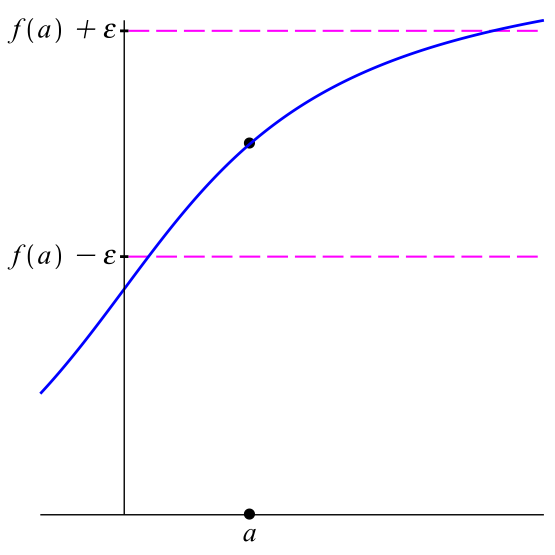
\includegraphics[width=\linewidth]{external/Continuity_1.pdf}
\end{sbspanel}%
\begin{sbspanel}{0.5}%
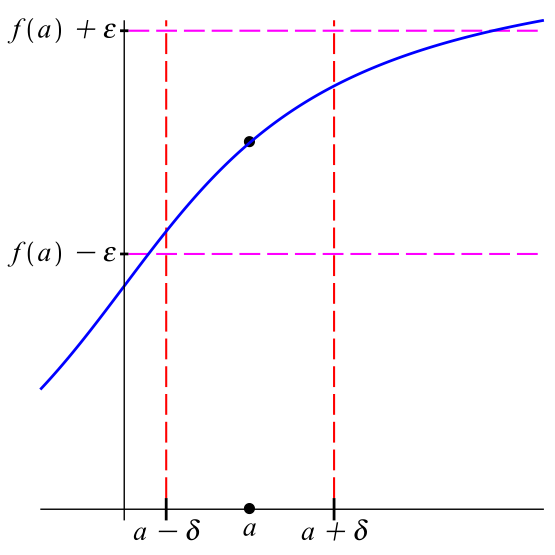
\includegraphics[width=\linewidth]{external/Continuity_2.pdf}
\end{sbspanel}%
\end{sidebyside}%
\tcblower
\end{figureptx}%
Let's deal with the first statement, making the values of \(f(x)\) ``as close to \(f(a)\) as we want''. What this means is that if we set any tolerance, say \(0.0001\), then we can make the values of \(f(x)\) within \(0.0001\) of \(f(a)\). Since the absolute value \(| f(x)-f(a) |\) measures how close \(f(x)\) is to \(f(a)\), we can rewrite the statement that the values of \(f(x)\) are within \(0.0001\) of \(f(a)\) as \(| f(x) - f(a) | \lt  0.0001\). Of course, \(0.0001\) may not be as close as we want to \(f(a)\), so we need a way to indicate that we can make the values of \(f(x)\) arbitrarily close to \(f(a)\) \textemdash{} within any tolerance at all. We do this by making the tolerance a parameter, \(\epsilon\). Then our job is to make the values of \(f(x)\) within \(\epsilon\) of \(f(a)\) regardless of the size of \(\epsilon\). We write this as%
\begin{equation*}
| f(x) - f(a) | \lt  \epsilon\text{.}
\end{equation*}
%
\par
We can picture this as shown at left in \hyperref[figure-F_Continuity]{Figure~{\xreffont\ref{figure-F_Continuity}}}. Here we want to make the values of \(f(x)\) lie within an \(\epsilon\) band of \(f(a)\) above and below \(f(a)\). That is, we want to be able to make the values of \(f(x)\) lie between \(f(a)-\epsilon\) and \(f(a)+\epsilon\).%
\par
Now we have to address the question of how we ``make'' the values of \(f(x)\) to be within \(\epsilon\) of \(f(a)\). Since the values \(f(x)\) are the dependent values, dependent on \(x\), we ``make'' the values of \(f(x)\) have the property we want by choosing the inputs \(x\) appropriately. In order for \(f\) to be continuous at \(x=a\), we must be able to find \(x\) values close enough to \(a\) to force \(| f(x) - f(a) | \lt \epsilon\). Pictorially, we can see how this might happen in the image at right in \hyperref[figure-F_Continuity]{Figure~{\xreffont\ref{figure-F_Continuity}}}. We need to be able to find an interval around \(x=a\) so that the graph of \(f(x)\) lies in the \(\epsilon\) band around \(f(a)\) for values of \(x\) in that interval. In other words, we need to be able to find some positive number \(\delta\) so that if \(x\) is in the interval \((a-\delta,
a+\delta)\), then the graph of \(f(x)\) lies in the \(\epsilon\) band around \(y=f(a)\). More formally, if we are given any positive tolerance \(\epsilon\), we must be able to find a positive number \(\delta\) so that if \(| x-a | \lt \delta\) (that is, \(x\) is in the interval \((a-\delta, a+\delta)\)), then \(| f(x) - f(a) | \lt \epsilon\) (or \(f(x)\) lies in the \(\epsilon\) band around \(y=f(a)\)).%
\par
This gives us a rigorous definition of what it means for a function \(f: \R \to \R\) to be continuous at a point.%
\begin{definition}{Definition}{}{definition-def_epsilon_delta_continuity}%
A function \(f : \R \to \R\) is \terminology{continuous at a point \(a\)} if, given any \(\epsilon \gt 0\), there exists a \(\delta \gt 0\) so that \(| x - a | \lt \delta\) implies \(| f(x) - f(a)| \lt \epsilon\).%
\end{definition}
Note that the value of \(\delta\) can depend on the value of \(a\) and on \(\epsilon\), but not on values of \(x\).%
\begin{exploration}{Preview Activity}{}{exploration-pa_MS_continuity}%
The \href{https://www.geogebra.org/m/rym36sqs}{GeoGebra file online}\footnotemark{} will allow us to play around with this definition. Use this GeoGebra applet for the first two problems in this activity.%
\begin{enumerate}[font=\bfseries,label=(\alph*),ref=\alph*]%
\item{}Enter \(f(x)=x\sin(x)\) as your function. (You can change the viewing window coordinates, the base point \(a\), and the function using the input boxes at the left on the screen.) Determine a value of \(\delta\) so that \(| f(x) - f(1) | \lt 0.5\) whenever \(| x - 1 | \lt \delta\). Explain your method.%
\item{}Now find a value of \(\delta\) so that \(| f(x) - f(2.5) | \lt 0.25\) whenever \(| x - 2.5 | \lt \delta\). Explain your method.%
\item{}\begin{enumerate}[font=\bfseries,label=(\roman*),ref=\theenumi.\roman*]%
\item{}What is the negation of the definition of continuity at a point? In other words, what do we need to do to show that a function \(f: \R \to \R\) is not continuous at a point \(x=a\)?%
\item{}Use the negation of the definition to explain why the function \(f : \R \to \R\) defined by%
\begin{equation*}
f(x) = \begin{cases}-1 \amp \text{ if }  x \lt  1 \\ 1 \amp \text{ if }  x \geq 1 \end{cases}
\end{equation*}
is not continuous at \(x=1\).%
\end{enumerate}%
\end{enumerate}%
\end{exploration}%
\footnotetext[5]{\nolinkurl{geogebra.org/m/rym36sqs}\label{fn-pa_MS_continuity-a-a-b}}%
\end{sectionptx}
%
%
\typeout{************************************************}
\typeout{Section  Continuous Functions Between Metric Spaces}
\typeout{************************************************}
%
\begin{sectionptx}{Section}{Continuous Functions Between Metric Spaces}{}{Continuous Functions Between Metric Spaces}{}{}{section-sec_cont_func_btwn}
In our preview activity we saw how to formally define what it means for a function \(f : \R \to \R\) to be continuous at a point.%
\par
Note that \hyperref[definition-def_epsilon_delta_continuity]{Definition~{\xreffont\ref{definition-def_epsilon_delta_continuity}}} depends only on being able to measure how close points are to each other. Since that is precisely what a metric does, we can extend this notion of continuity to define continuity for functions between metric spaces. Continuity is an important idea in topology, and we will work with this idea extensively throughout the semester.%
\par
If we let \(d_E : \R \times \R \to \R\) be defined by \(d_R(x,y) = | x - y |\), then we have seen that \(d_E\) is a metric on \(\R\) (note that \(d_E\) is the Euclidean metric on \(\R\)). Using this metric we can reformulate what it means for a function \(f : \R \to \R\) to be continuous at a point.%
\begin{definition}{Definition}{Alternate Definition.}{definition-sec_cont_func_btwn-e}%
A function \(f : \R \to \R\) is \terminology{continuous at a point \(a\)} if, given any \(\epsilon \gt 0\), there exists a \(\delta \gt 0\) so that \(d_E(x,a) \lt \delta\) implies \(d_E(f(x), f(a)) \lt \epsilon\).%
\end{definition}
This alternate definition depends on the metric \(d_E\). We could easily replace the metric \(d\) with any other metric we choose. This allows us to define continuity at a point for functions between metric spaces.%
\begin{definition}{Definition}{}{definition-sec_cont_func_btwn-g}%
\index{continuity at a point in a metric space}%
Let \((X,d_X)\) and \((Y, d_Y)\) be metric spaces. A function \(f:X \to Y\) is \terminology{continuous} at \(a \in X\) if, given any \(\epsilon \gt 0\), there exists a \(\delta \gt 0\) so that \(d_X(x,a)\lt \delta\) implies \(d_Y(f(x), f(a)) \lt \epsilon\).%
\end{definition}
Once we have defined continuity at a point, we can define continuous functions.%
\begin{definition}{Definition}{}{definition-sec_cont_func_btwn-i}%
\index{continuous function}%
Let \((X,d_X)\) and \((Y, d_Y)\) be metric spaces. A function \(f:X \to Y\) is \terminology{continuous} if \(f\) is continuous at every point in \(X\).%
\end{definition}
\begin{example}{Example}{}{example-sec_cont_func_btwn-j}%
In general, to prove that a function \(f:X \to Y\) is continuous, where \((X,d_X)\) and \((Y, d_Y)\) are metric spaces, we begin by choosing an arbitrary element \(a\) in \(X\). Then we let \(\epsilon\) be a number greater than \(0\) and show that there is a \(\delta \gt 0\) so that \(d_Y(f(x),f(a)) \lt  \epsilon\) whenever \(d_X(x,a) \lt  \delta\). The \(\delta\) we need cannot depend on \(x\) (since \(x\) isn't known), but can depend on the value of \(a\) that we choose, and will likely depend on \(\epsilon\) as well. That is, there is a function \(C\) of only the independent variables \(a\) and \(\epsilon\) that produces the \(\delta\), or \(\delta = C(a,\epsilon)\). As an example, let \(X = \R\) and let \(d_X\) be defined as%
\begin{equation*}
d_X(x,y) = \min\{|x-y|,1\}\text{.}
\end{equation*}
%
\par
The proof that \(d_X\) is a metric is left for \hyperlink{exercise-ex_min_1_metric}{Exercise~{\xreffont 9}}. Consider \(f : X \to Y\) defined by \(f(x) = x^2\), where \((Y,d_Y) = (\R, d_E)\). To show that \(f\) is continuous, we let \(a \in \R\) and let \(\epsilon \gt 0\).%
\begin{quote}%
\emph{Scratch work.} What happens next is not part of the proof, but shows how we go about finding a \(\delta\) we need. We are looking for \(\delta \gt 0\) such that \(d_X(x,a) \lt  \delta\) implies that \(d_E(f(x),f(a)) \lt  \epsilon\). That is, we want to make%
\begin{equation*}
d_E(f(x),f(a)) = \sqrt{(f(x)-f(a))^2} = |f(x)-f(a)| = |x^2-a^2| \lt  \epsilon
\end{equation*}
whenever%
\begin{equation*}
d_X(x,a) = \min\{|x-a|, 1\} \lt  \delta\text{.}
\end{equation*}
Now \(|x^2-a^2| = |(x-a)(x+a)| = |x-a| \ |x+a|\). If \(d_X(x,a) \lt  \delta\), then \(\min\{|x-a|, 1\} \lt  \delta\). If we choose \(\delta \lt  1\), then \(d_X(x,a) \lt  \delta \lt  1\) implies that \(|x-a| \lt  1\) and so \(d_X(x,a) = |x-a|\). Now%
\begin{equation*}
|x+a| = |(x-a) + 2a| \leq |x-a| + 2|a| \lt  1+2|a|\text{.}
\end{equation*}
It follows that%
\begin{equation*}
|x-a| \ |x+a| \lt  \delta(1+2|a|)\text{.}
\end{equation*}
To make this product less that \(\epsilon\), we can choose \(\delta\) such that \(\delta(1+2|a|) \lt  \epsilon\) or \(\delta \lt  \frac{\epsilon}{1+2|a|}\). That is, there is a function \(C\) of \(\epsilon\) that gives us the \(\delta\) we want, namely \(\delta = C(a,\epsilon) = \left\{1, \frac{\epsilon}{1+2|a|}\right\}\). Now we ignore this paragraph and present the proof, which is essentially reversing the steps we just made. If the steps can't be reversed, then we have to rethink our argument. The next step in the proof might seem like magic to the uninitiated reader, but we have seen behind the curtain so it isn't a mystery to us.%
\end{quote}
Let \(\delta\) be a positive number less than \(\min\left\{1, \frac{\epsilon}{1+2|a|}\right\}\). Then%
\begin{equation*}
d_X(x,a) = \min\{|x-a|,1\} \lt  \delta
\end{equation*}
implies that \(d_X(x,a) \lt  \delta \lt  1\) and so \(d_X(x,a) = |x-a| \lt  \delta \lt  1\). Then%
\begin{equation*}
|x+a| = |(x-a) + 2a| \leq |x-a| + 2|a| \lt  1+2|a|\text{.}
\end{equation*}
%
\par
It follows that%
\begin{align*}
d_E(f(x),f(a)) \amp = \sqrt{(f(x)-f(a))^2}\\
\amp = |f(x)-f(a)|\\
\amp = |x^2-a^2|\\
\amp = |(x-a)(x+a)|\\
\amp = |x-a| \ |x+a|\\
\amp \lt  \delta (1+2|a|)\\
\amp \lt   \left(\frac{\epsilon}{1+2|a|}\right) (1+2|a|)\\
\amp = \epsilon\text{.}
\end{align*}
%
\par
We conclude that \(f\) is continuous at every point in \(X\) and so \(f\) is a continuous function.%
\end{example}
Not all functions are continuous as we see in the next example.%
\begin{example}{Example}{}{example-exp_not_continuous}%
Let \(X = Y = \R\) and define \(f : X \to Y\) by \(f(x) = x\). Let \(d_X\) be the Euclidean metric and \(d_Y\) the discrete metric. (Recall that \(d_Y(x,y) = 1\) whenever \(x \neq y\).) Let \(a \in X\) and let \(0 \lt \epsilon \lt 1\).%
\par
Let \(\delta \gt 0\), and let \(x = a+\frac{\delta}{2}\). Then \(x \neq a\) and \(d_X(x,a) \lt  \delta\). However,%
\begin{equation*}
d_Y(f(x),f(a)) = d_Y(x,a) = 1\text{.}
\end{equation*}
%
\par
So if \(0 \lt \epsilon \lt 1\), there is no \(\delta \gt 0\) such that \(d_X(x,a) \lt \delta\) implies that \(d_Y(f(x),f(a)) \lt \epsilon\). We conclude that \(f\) is continuous at no point in \(X\).%
\end{example}
Certain functions are always continuous, as the next activity shows.%
\begin{activity}{Activity}{}{activity-act_id_constant_continuous}%
\begin{enumerate}[font=\bfseries,label=(\alph*),ref=\alph*]%
\item{}Let \((X, d_X)\) and \((Y, d_Y)\) be metric spaces, and let \(b \in Y\). Define \(f : X \to Y\) by \(f(x) = b\) for every \(x \in X\). Show that \(f\) is a continuous function.%
\item{}Let \((X, d)\) be a metric space. Define the function \(i_X : X \to X\) by \(i_X(x) = x\) for every \(x \in X\). Show that \(i_X\) is a continuous function. (The function \(i_X\) is called the \terminology{identity function} \index{identity function} on \(X\).)%
\item{}Why doesn't the argument in part (b) contradict \hyperref[example-exp_not_continuous]{Example~{\xreffont\ref{example-exp_not_continuous}}}?%
\end{enumerate}%
\end{activity}%
More complicated examples are in the next activity.%
\begin{activity}{Activity}{}{activity-sec_cont_func_btwn-p}%
Let \(X = (\R^2, d_T)\) and \(Y = (\R^2, d_M)\), where%
\begin{equation*}
d_T((x_1, x_2), (y_1,y_2)) = | x_1-y_1 | + | x_2-y_2 |
\end{equation*}
is the taxicab metric and%
\begin{equation*}
d_M((x_1, x_2), (y_1,y_2)) = \max\{| x_1-y_1 |,  | x_2-y_2 |\}
\end{equation*}
is the max metric. Define \(f : \R^2 \to \R^2\) by \(f((a,b)) = (a+b, b)\).%
\begin{enumerate}[font=\bfseries,label=(\alph*),ref=\alph*]%
\item{}Is \(f\) a continuous function from \(X\) to \(Y\)? Justify your answer.%
\item{}Is \(f\) a continuous function from \(Y\) to \(X\)? Justify your answer.%
\end{enumerate}%
\end{activity}%
\end{sectionptx}
%
%
\typeout{************************************************}
\typeout{Section  Composites of Continuous Functions}
\typeout{************************************************}
%
\begin{sectionptx}{Section}{Composites of Continuous Functions}{}{Composites of Continuous Functions}{}{}{section-sec_comp_cont_func}
Let \((X, d_X)\), \((Y,d_Y)\), and \((Z, d_Z)\) be metric spaces, and suppose \(f: X \to Y\) and \(g: Y \to Z\) are continuous functions. It seems natural to ask if the composite \(g \circ f : X \to Z\) is a continuous function.%
\begin{activity}{Activity}{}{activity-sec_comp_cont_func-c}%
Let \((X, d_X)\), \((Y,d_Y)\), and \((Z, d_Z)\) be metric spaces, and suppose \(f: X \to Y\) and \(g: Y \to Z\) are continuous functions. We will prove that \(g \circ f\) is a continuous function.%
\begin{enumerate}[font=\bfseries,label=(\alph*),ref=\alph*]%
\item{}What do we have to do to show that \(g \circ f\) is a continuous function? What are the first two steps in our proof?%
\item{}Let \(a \in X\) and let \(b = f(a)\). Suppose \(\epsilon \gt 0\) is given. Explain why there must exist a \(\delta_1 \gt 0\) so that \(d_Y(y,b) \lt \delta_1\) implies \(d_Z(g(y), g(b)) \lt \epsilon\).%
\item{}Now explain why there exists a \(\delta_2 \gt 0\) so that \(d_X(x,a) \lt \delta_2\) implies that \(d_Y(f(x),
f(a)) \lt \delta_1\).%
\item{}Prove that \(g \circ f : X \to Z\) is a continuous function.%
\end{enumerate}%
\end{activity}%
Continuity is an important concept in topology. We have seen how to define continuity in metric spaces, and we will soon expand on this idea to define continuity without reference to metrics at all. This will allow us to later define continuous functions between arbitrary topological spaces.%
\end{sectionptx}
%
%
\typeout{************************************************}
\typeout{Section  Summary}
\typeout{************************************************}
%
\begin{sectionptx}{Section}{Summary}{}{Summary}{}{}{section-sec_cont_func_summ}
Important ideas that we discussed in this section include the following.%
\begin{itemize}[label=\textbullet]
\item{}Let \((X,d_X)\) and \((Y, d_Y)\) be metric spaces. A function \(f:X \to Y\) is continuous at \(a \in X\) if, given any \(\epsilon \gt 0\), there exists a \(\delta \gt 0\) so that \(d_X(x,a)\lt \delta\) implies \(d_Y(f(x), f(a)) \lt \epsilon\).%
\item{}Let \((X,d_X)\) and \((Y, d_Y)\) be metric spaces. A function \(f:X \to Y\) is continuous if \(f\) is continuous at every point in \(X\).%
\end{itemize}
%
\end{sectionptx}
%
%
\typeout{************************************************}
\typeout{Exercises  Exercises}
\typeout{************************************************}
%
\begin{exercises-section}{Exercises}{Exercises}{}{Exercises}{}{}{exercises-sec_cont_func_exer}
\begin{divisionexercise}{1}{}{}{exercise-sec_cont_func_exer-a}%
Let \(f: \R \to \R\) be defined by \(f(x) = |x|\), with the Euclidean metric on both the domain and the codomain. Is \(f\) continuous at \(x=0\)? Prove your answer.%
\end{divisionexercise}%
\begin{divisionexercise}{2}{}{}{exercise-sec_cont_func_exer-b}%
Let \(f: \R \to \R\) be defined by \(f(x) = \begin{cases}\frac{x}{|x|} \amp \text{ if } x \neq 0 \\ 1 \amp \text{ if } x=0. \end{cases}\) Is \(f\) continuous at \(x=0\)? Prove your answer.%
\end{divisionexercise}%
\begin{divisionexercise}{3}{}{}{exercise-sec_cont_func_exer-c}%
Let \((Y, d_Y) = (\R, d_E)\), where \(d_E\) is the Euclidean metric.%
\begin{enumerate}[font=\bfseries,label=(\alph*),ref=\alph*]%
\item{}Let \((X,d_X) = (\R^2, d_E)\). Prove or disprove: the function \(f:X \to Y\) defined by \(f((x_1,x_2)) = x_1 + x_2\) is continuous.%
\item{}Let \((X,d_X) = (\R^2, d_M)\) where \(d_M\) is the max metric. Prove or disprove: the function \(f:X \to Y\) defined by \(f((x_1,x_2)) = x_1 + x_2\) is continuous.%
\end{enumerate}%
\end{divisionexercise}%
\begin{divisionexercise}{4}{}{}{exercise-sec_cont_func_exer-d}%
Let \(X\) be any set and define \(d : X \times X \to \R\) by%
\begin{equation*}
d(x,y) = \begin{cases}0 \amp \text{ if }  x=y \\ 1 \amp \text{ if }  x \neq y. \end{cases}
\end{equation*}
\hyperlink{exercise-ex_MS_discrete}{Exercise~{\xreffont 1}} asks us to show that \(d\) is a metric (the discrete metric) on \(\R\). Let \((X,d_X)\) and \((Y, d_Y)\) be metric spaces with \(d_X\) the discrete metric. Determine all of the continuous functions \(f\) from \(X\) to \(Y\).%
\end{divisionexercise}%
\begin{divisionexercise}{5}{}{}{exercise-ex_sum_continuous}%
Let \(f\) and \(g\) be continuous functions from \((\R,d_E)\) to \((\R, d_E)\).%
\begin{enumerate}[font=\bfseries,label=(\alph*),ref=\alph*]%
\item{}Let \(k \in \R\) with \(k \neq 0\) and define \(kf : \R \to \R\) by \((kf)(x) = kf(x)\) for all \(x \in \R\). Show that \(kf\) is a continuous function.%
\item{}Define \(f+g : \R \to \R\) by \((f+g)(x) = f(x) + g(x)\) for all \(x \in \R\). Show that \(f+g\) is a continuous function.%
\end{enumerate}%
\end{divisionexercise}%
\begin{divisionexercise}{6}{}{}{exercise-sec_cont_func_exer-f}%
Let \(f\) and \(g\) be continuous functions from \((\R, d_E)\) to \((\R,d_E)\). In this exercise we will prove that \(fg\) is a continuous function from \(\R\) to \(\R\). Let \(a\) be in \(\R\), and follow the steps below to show that \(fg\) is continuous at \(x=a\). Let \(\epsilon\) be a positive number.%
\begin{enumerate}[font=\bfseries,label=(\alph*),ref=\alph*]%
\item{}We will first want to express \(f(x)g(x) - f(a)g(a)\) in a more useful way. Use the fact that \(f(x) = f(a) + (f(x)-f(a))\) and \(g(x)  = g(a) + (g(x)-g(a))\) to show that%
\begin{align*}
f(x)g(x)-f(a)g(a) = f(a)(g(x)-g(a)) \amp + g(a)(f(x)-f(a))\\
\amp + (f(x)-f(a))(g(x)-g(a))\text{.}
\end{align*}
%
\item{}Explain why there exist positive numbers \(\delta_1\), \(\delta_2\), \(\delta_3\), and \(\delta_4\) such that%
\begin{align*}
|f(x)-f(a)| \lt  \sqrt{\frac{\epsilon}{3}} \amp \text{ when }  |x-a| \lt  \delta_1\\
|g(x)-g(a)| \lt   \sqrt{\frac{\epsilon}{3}}  \amp \text{ when }  |x-a| \lt  \delta_2\\
|f(x)-f(a)| \lt  \frac{\epsilon}{3(1+|g(a)|)}  \amp \text{ when }  |x-a| \lt  \delta_3\\
|g(x)-g(a)| \lt  \frac{\epsilon}{3(1+|f(a)|)}  \amp \text{ when }  |x-a| \lt  \delta_4\text{.}
\end{align*}
%
\item{}Use the results of (a) and (b) to show that \(fg\) is continuous at \(x=a\). (Hint: \(1+|f(a)| \gt |f(a)|\).)%
\end{enumerate}%
\end{divisionexercise}%
\begin{divisionexercise}{7}{}{}{exercise-sec_cont_func_exer-g}%
Let \(f\) and \(g\) be functions from \((\R,d_E)\) to \((\R,d_E)\).%
\begin{enumerate}[font=\bfseries,label=(\alph*),ref=\alph*]%
\item{}Is it true that if \(f+g\) is a continuous function, then \(f\) and \(g\) are continuous functions? Verify your answer.%
\item{}Is it true that if \(fg\) is a continuous function, then \(f\) and \(g\) are continuous functions? Verify your answer.%
\end{enumerate}%
\end{divisionexercise}%
\begin{divisionexercise}{8}{}{}{exercise-sec_cont_func_exer-h}%
Let \(f(x) = 2x^2+1\) map from \(\R\) to \(\R\), with both the domain and codomain having the Euclidean metric.%
\begin{enumerate}[font=\bfseries,label=(\alph*),ref=\alph*]%
\item{}Let \(\epsilon = \frac{1}{4}\). Find a value of \(\delta\) such that \(|x-1| \lt \delta\) implies that \(|f(x)-f(a)| \lt \epsilon\). You might use the applet at to confirm your value of \(\delta\).%
\item{}Prove that \(f\) is continuous at \(x=1\).%
\end{enumerate}%
\end{divisionexercise}%
\begin{divisionexercise}{9}{}{}{exercise-ex_min_1_metric}%
Define \(d: \R \times \R \to \R\) as%
\begin{equation*}
d(x,y) = \min\{|x-y|,1\}\text{.}
\end{equation*}
Prove that \(d\) is a metric.%
\end{divisionexercise}%
\begin{divisionexercise}{10}{}{}{exercise-sec_cont_func_exer-j}%
Let \(f : \R \to \R\) be a continuous function, with both copies of \(\R\) having the Euclidean metric. Assume that \(f(x) = 0\) whenever \(x\) is rational. Prove that \(f(x) = 0\) for every \(x \in \R\).%
\par\smallskip%
\noindent\textbf{\blocktitlefont Hint}.\hypertarget{hint-sec_cont_func_exer-j-b}{}\quad{}Use \hyperlink{exercise-ex_GLB_rational}{Exercise~{\xreffont 7}}.%
\end{divisionexercise}%
\begin{divisionexercise}{11}{}{}{exercise-sec_cont_func_exer-k}%
Let \(f: \R \to \R\) be defined by \(f(x) = 0\) if \(x\) is irrational and \(f(x) = 1\) if \(x\) is rational. Assume the Euclidean metric on both copies of \(\R\). Show that \(f\) is not continuous at any point in \(\R\).%
\par\smallskip%
\noindent\textbf{\blocktitlefont Hint}.\hypertarget{hint-sec_cont_func_exer-k-b}{}\quad{}Use \hyperlink{exercise-ex_GLB_rational}{Exercise~{\xreffont 7}} and \hyperlink{exercise-ex_GLB_irrational}{Exercise~{\xreffont 10}}.%
\end{divisionexercise}%
\begin{divisionexercise}{12}{}{}{exercise-sec_cont_func_exer-l}%
Let \(g: \R \to \R\) be defined by \(g(x) = 0\) if \(x\) is irrational and \(g(x) = x\) if \(x\) is rational. Assume the Euclidean metric on both copies of \(\R\). Show that \(g\) is continuous only at \(0\).%
\end{divisionexercise}%
\begin{divisionexercise}{13}{}{}{exercise-sec_cont_func_exer-m}%
Let \(X\) be the set of continuous functions \(f: [a,b] \to \mathbb{R}\). Let \(d^*\) be the distance function on \(X\) defined by%
\begin{equation*}
d^*(f,g)= \int_a^b \la f(t)-g(t) \ra \, dt\text{,}
\end{equation*}
for \(f, g \in X\). For each \(f \in X\), set%
\begin{equation*}
I(f) = \int_a^b f(t) \, dt\text{.}
\end{equation*}
%
\begin{enumerate}[font=\bfseries,label=(\alph*),ref=\alph*]%
\item{}Determine the value of \(d^*(f,g)\) when \(f(x) = x^2\), \(g(x) = 3-2x\), and \([a,b] = [-3,3]\).%
\item{}Determine the value of \(I(f)\) if \(f(x) = 2x\) and \([a,b] = [0,2]\).%
\item{}Prove that the function \(I : (X, d^*) \to (\R,d)\) is continuous, where \(d\) is the Euclidean metric.%
\par\smallskip%
\noindent\textbf{\blocktitlefont Hint}.\hypertarget{hint-sec_cont_func_exer-m-d-b}{}\quad{}It helps to start by explicitly writing down what it means for \(I\) to be continuous in terms of the metrics \(d^*\) and \(d\) before trying to prove this statement.%
\end{enumerate}%
\end{divisionexercise}%
\begin{divisionexercise}{14}{}{}{exercise-sec_cont_func_exer-n}%
For each of the following, answer true if the statement is always true. If the statement is only sometimes true or never true, answer false and provide a concrete example to illustrate that the statement is false. If a statement is true, explain why.%
\begin{enumerate}[font=\bfseries,label=(\alph*),ref=\alph*]%
\item{}Let \(f : X \to Y\) be a function, where \((X, d_X)\) and \((Y, d_Y)\) are metric spaces. If \(d_X\) is the discrete metric and \(d_Y\) is any metric, then \(f\) is continuous.%
\item{}Let \(f : X \to Y\) be a function, where \((X, d_X)\) and \((Y, d_Y)\) are metric spaces. If \(d_Y\) is the discrete metric and \(d_X\) is any metric, then \(f\) is continuous.%
\item{}Let \(d_1\) and \(d_2\) be two metrics on a set \(X\). The identity function \(i_X : (X,d_1) \to (X,d_2)\) defined by \(i_X(x) = x\) for every \(x \in X\) is continuous.%
\item{}Let \(f\) and \(g\) be continuous functions from \((\R^2, d_T)\) (the taxicab metric) to \((\R,d_E)\). Then the function \(f+g\) from \((\R^2, d_T)\) to \((\R,d_E)\) defined by \((f+g)(x) = f(x) + g(x)\) for every \(x \in \R^2\) is a continuous function.%
\item{}If \((X, d_X)\) and \((Y,d_Y)\) are metric spaces with \(y \in Y\), then the constant function \(f: X \to Y\) defined by \(f(x) = y\) for every \(x \in X\) is a continuous function.%
\end{enumerate}%
\end{divisionexercise}%
\end{exercises-section}
\end{chapterptx}
 %
%
\typeout{************************************************}
\typeout{Chapter 7 Open Balls and Neighborhoods in Metric Spaces}
\typeout{************************************************}
%
\begin{chapterptx}{Chapter}{Open Balls and Neighborhoods in Metric Spaces}{}{Open Balls and Neighborhoods in Metric Spaces}{}{}{chapter-chap_open_balls}
\renewcommand*{\chaptername}{Chapter}
\begin{objectives}{Focus Questions}{objectives-chap_open_balls-b}
%
\begin{itemize}[label=\textbullet]
\item{}What is an open ball in a metric space? Give one important property of open balls.%
\item{}What is a neighborhood of a point in a metric space?%
\item{}How can we use open balls or neighborhoods to determine the continuity of a function at a point?%
\end{itemize}
\end{objectives}
%
%
\typeout{************************************************}
\typeout{Section  Introduction}
\typeout{************************************************}
%
\begin{sectionptx}{Section}{Introduction}{}{Introduction}{}{}{section-sec_open_balls_intro}
Open sets are vitally important in topology. We will see later that every topological space is completely defined by its open sets, and continuous functions can be defined just in terms of open sets. In this section we introduce the idea of open balls and neighborhoods in metric spaces and discover a few of their properties. This discussion will form the basis for introducing open sets in the next section.%
\par
Recall that the continuity of a function \(f\) from a metric space \((X, d_X)\) to a metric space \((Y, d_Y)\) at a point \(a\) is defined in terms of sets of points \(x \in X\) such that \(d_X(x,a) \lt \delta\) and \(y \in Y\) such that \(d_Y(y, f(a)) \lt \epsilon\) for positive real numbers \(\delta\) and \(\epsilon\). In \(\R\) with the Euclidean metric \(d_E\), for real numbers \(x\) and \(a\) the set of \(x\) values satisfying \(d_E(x,a) \lt \delta\) is the set of \(x\) values so that \(| x-a | \lt \delta\). We often write this set in interval notation as \((a-\delta,
a+\delta)\) and call \((a-\delta,
a+\delta)\) an open interval. An informal reason that we call such an interval open (as opposed to the intervals \([a-\delta,
a+\delta)\), \((a-\delta, a+\delta]\), or \([a-\delta,
a+\delta]\)) is that the open interval does not contain either of its endpoints. A more substantial reason to call such an interval open is that if \(x'\) is any element in \((a-\delta,
a+\delta)\), then we can find another open interval around \(x'\) that is completely contained in the interval \((a-\delta,
a+\delta)\). So you could naively think of an open interval as one in which there is enough room in the interval for any point in the interval to wiggle around a bit and stay within the interval.%
\par
Since the open interval \((a-\delta,
a+\delta)\) can be described completely by the Euclidean metric as the set of \(x\) values so that \(d_E(x,a) \lt \delta\), there is no reason why we can't extend this notation of open interval to any metric space. We must note, though, that \(\R\) is one-dimensional while most metric spaces are not, so the term ``interval'' will no longer be appropriate. We replace the concept of interval with that of an open ball.%
\begin{definition}{Definition}{}{definition-sec_open_balls_intro-e}%
\index{open ball in a metric space}%
Let \((X, d_X)\) be a metric space, and let \(a \in X\). For \(\delta \gt 0\), the \terminology{open ball \(B(a, \delta)\) of radius \(\delta\) around \(a\)} is the set%
\begin{equation*}
B(a, \delta) = \{x \in X \mid d_X(x,a) \lt  \delta\}\text{.}
\end{equation*}
%
\end{definition}
We note here that our notation for an open ball is not universal. For example, some texts use \(B_{\delta}(a)\) for our \(B(a,\delta)\).%
\begin{exploration}{Preview Activity}{}{exploration-sec_open_balls_intro-g}%
Describe and draw a picture of the indicated open ball in each of the following metric spaces.%
\begin{enumerate}[font=\bfseries,label=(\alph*),ref=\alph*]%
\item{}The open ball \(B(2, 1)\) in the metric space \((\R, d_E)\) with the Euclidean metric%
\begin{equation*}
d_E(x,y) = | x-y |\text{.}
\end{equation*}
%
\item{}The open ball \(B((3,2), 1)\) in the metric space \((\R^2, d_E)\) with the Euclidean metric%
\begin{equation*}
d_E((x_1,x_2),(y_1,y_2)) = \sqrt{(x_1-y_1)^2 + (x_2-y_2)^2}\text{.}
\end{equation*}
%
\item{}The open ball \(B((3,2), 1)\) in the metric space \((\R^2, d_M)\) with the max metric%
\begin{equation*}
d_M((x_1,x_2),(y_1,y_2)) = \max\{| x_1-y_1 |, | x_2-y_2 |\}\text{.}
\end{equation*}
%
\item{}The open ball \(B((3,2), 1)\) in the metric space \((\R^2, d_T)\) with the taxicab metric%
\begin{equation*}
d_T((x_1,x_2),(y_1,y_2)) = | x_1-y_1 | + | x_2-y_2 |\text{.}
\end{equation*}
%
\item{}The open ball \(B((3,2), 1)\) in the metric space \((\R^2, d)\) with the discrete metric%
\begin{equation*}
d(x,y) = \begin{cases}0 \amp \text{ if }  x=y \\ 1 \amp \text{ if }  x \neq y. \end{cases}\text{.}
\end{equation*}
What is the difference between \(B((3,2),1)\) and \(B((3,2),r)\) in this metric space if \(r > 1\)? If \(r \lt  1\)?%
\end{enumerate}%
\end{exploration}%
\end{sectionptx}
%
%
\typeout{************************************************}
\typeout{Section  Neighborhoods}
\typeout{************************************************}
%
\begin{sectionptx}{Section}{Neighborhoods}{}{Neighborhoods}{}{}{section-sec_neighborhoods}
\index{\(\delta\)-neighborhood of a point in a metric space}%
We are familiar with the idea of open intervals in \(\R\). We next introduce the idea of an open neighborhood of a point and characterize continuity in terms of neighborhoods. This is the next step in developing the notation of continuity in topological spaces.%
\par
The open ball \(B(a, \delta)\) in a metric space \((X,d)\) is also called the \terminology{\(\delta\)-neighborhood} around \(a\). A neighborhood of a point can be thought of as any set that envelops that point.%
\begin{definition}{Definition}{}{definition-sec_neighborhoods-e}%
\index{neighborhood in a metric space}%
Let \((X, d_X)\) be a metric space, and let \(a \in X\). A subset \(N\) of \(X\) is a \terminology{neighborhood} of \(a\) if there exists a \(\delta \gt 0\) such that \(B(a, \delta) \subseteq N\).%
\end{definition}
\begin{example}{Example}{}{example-exp_neighborhood_MS}%
%
\begin{itemize}[label=\textbullet]
\item{}In \(\R\) with the Euclidean metric, the set \(\R^+\) (the positive real numbers) is a neighborhood of \(a=1\) because the open ball \(B(1,0.5)\) is completely contained in \(\R^+\).%
\item{}In \(\R\) with the Euclidean metric, the set \(\Z\) is not a neighborhood of \(a=1\) because any open ball centered at \(a=1\) will contain some non-integers.%
\item{}In \(\R\) with the discrete metric, the set \(\Z\) is a neighborhood of \(a=1\) because the open ball \(B(a,1) = \{a\}\).%
\end{itemize}
%
\end{example}
As another example, the open ball \(B(a, \delta)\) is a neighborhood of \(a\). We can say even more about open balls.%
\begin{activity}{Activity}{}{activity-sec_neighborhoods-h}%
Let \((X, d)\) be a metric space, let \(a \in X\), and let \(\delta \gt 0\). In this activity we ask the question, is \(B(a, \delta)\) a neighborhood of each of its points?%
\begin{enumerate}[font=\bfseries,label=(\alph*),ref=\alph*]%
\item{}Let \(b \in B(a, \delta)\). What do we have to do to show that \(B(a, \delta)\) is a neighborhood of \(b\)?%
\item{}Use \hyperref[figure-F_Open_ball_neighborhood]{Figure~{\xreffont\ref{figure-F_Open_ball_neighborhood}}} to help show that \(B(a, \delta)\) is a neighborhood of \(b\).%
\begin{figureptx}{Figure}{\(B(a, \delta)\) as a neighborhood of \(b\).}{figure-F_Open_ball_neighborhood}{}%
\begin{image}{0.25}{0.5}{0.25}{}%
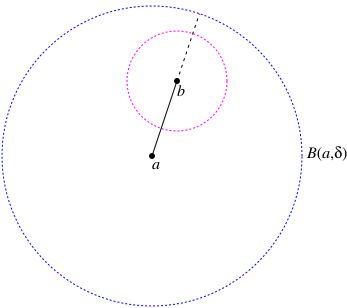
\includegraphics[width=\linewidth]{external/Open_ball_neighborhood.pdf}
\end{image}%
\tcblower
\end{figureptx}%
\item{}Is the converse true? That is, if a set is a neighborhood of each of its points, is the set an open ball? No proof is necessary, but a convincing argument is in order.%
\end{enumerate}%
\end{activity}%
\end{sectionptx}
%
%
\typeout{************************************************}
\typeout{Section  Continuity and Neighborhoods}
\typeout{************************************************}
%
\begin{sectionptx}{Section}{Continuity and Neighborhoods}{}{Continuity and Neighborhoods}{}{}{section-sec_cont_neighborhoods}
We can define continuity now in terms of neighborhoods instead of using metrics. The advantage here is that this idea does not explicitly depend on the existence of a metric, so we will be able to adopt this concept of continuity for arbitrary topological spaces.%
\par
Recall that a function \(f\) from a metric space \((X, d_X)\) to a metric space \((Y, d_Y)\) is continuous at \(a \in X\) if, for any \(\epsilon \gt 0\) there exists \(\delta \gt 0\) so that \(d_X(x,a) \lt \delta\) implies \(d_Y(f(x),f(a)) \lt \epsilon\). We can interpret this definition of continuity to say that for every \(\epsilon \gt 0\), the inverse image under \(f\) of the open ball \(B(f(a), \epsilon)\) contains the open ball \(B(a, \delta)\) for some \(\delta \gt 0\). It is not unreasonable to wonder if the set \(f^{-1}\left(B(f(a), \epsilon)\right)\) itself is an open ball. We investigate this question in the following activity.%
\begin{activity}{Activity}{}{activity-act_OB_1}%
Let \(f\) be a function from a metric space \((X, d_X)\) to a metric space \((Y, d_Y)\) that is continuous at \(a \in X\). Using the notation from the paragraph above, in this activity we determine if \(f^{-1}\left(B(f(a), \epsilon)\right)\) must equal \(B(a, \delta)\) for some \(\delta\).%
\par
Define \(f : \R \to \R\) by%
\begin{equation*}
f(x) = x^2\text{,}
\end{equation*}
where we use the Euclidean metric \(d_E\) throughout. Assume that \(f\) is a continuous function. Then \(f\) is continuous at \(x=2\).%
\begin{enumerate}[font=\bfseries,label=(\alph*),ref=\alph*]%
\item{}What is \(B(f(2), 1)\)?%
\item{}What is \(f^{-1}\left(B(f(2), 1)\right)\)?%
\item{}Is \(f^{-1}\left(B(f(2), 1)\right)\) an open ball centered at \(2\)? Explain.%
\end{enumerate}%
\end{activity}%
The conclusion to be drawn from \hyperref[activity-act_OB_1]{Activity~{\xreffont\ref{activity-act_OB_1}}} is that if \(f\) is continuous, we can only conclude that the inverse image of \(B(f(a), \epsilon)\) \terminology{contains} an open ball centered at \(a\). By definition of continuity, if for every \(\epsilon \gt 0\) there exists a \(\delta \gt 0\) so that the open ball \(f^{-1}\left(B(f(a), \epsilon)\right)\) contains \(B(a, \delta)\), then \(f\) is continuous at \(a\). We summarize this in the next theorem.%
\begin{theorem}{Theorem}{}{}{theorem-thm_open_ball_continuity}%
Let \(f\) be a function a metric space \((X, d_X)\) to a metric space \((Y, d_Y)\), and let \(a \in X\). Then \(f\) is continuous at \(a \in X\) if and only if, given any \(\epsilon \gt 0\) there exists \(\delta \gt 0\) so that%
\begin{equation*}
B(a, \delta) \subseteq f^{-1}\left(B(f(a), \epsilon)\right)\text{.}
\end{equation*}
%
\end{theorem}
We can extend this idea of continuity to describe continuity in terms of neighborhoods. This condition will allow us to later consider continuous functions even if there are no metrics on our spaces.%
\begin{theorem}{Theorem}{}{}{theorem-sec_cont_neighborhoods-h}%
Let \((X, d_X)\) and \((Y,d_Y)\) be metric spaces, and let \(f : X \to Y\) be a function. Then \(f\) is continuous at \(a \in X\) if and only if the inverse image of every neighborhood of \(f(a)\) is a neighborhood of \(a\).%
\end{theorem}
\begin{proof}{Proof}{}{proof-sec_cont_neighborhoods-h-b}
Let \((X, d_X)\) and \((Y,d_Y)\) be metric spaces, and let \(f : X \to Y\) be a function. To prove this biconditional statement we need to prove both implications. First assume that \(f\) is continuous at some point \(a \in X\). We will show that for any neighborhood \(N\) of \(f(a)\) in \(Y\), its inverse image \(f^{-1}(N)\) in \(X\) is a neighborhood of \(a\) in \(X\). Let \(N\) be a neighborhood of \(f(a)\) in \(Y\). To demonstrate that \(f^{-1}(N)\) is a neighborhood of \(a\) in \(X\), we need to find an open ball around \(a\) that is contained in \(f^{-1}(N)\). Since \(N\) is a neighborhood of \(f(a)\), by definition there exists \(\epsilon \gt 0\) so that \(B(f(a), \epsilon) \subseteq N\). Since \(f\) is continuous at \(a\), there exists \(\delta \gt 0\) such that \(B(a, \delta) \subseteq f^{-1}\left(B(f(a), \epsilon)\right)\). So if \(x \in B(a, \delta)\), then \(f(x) \in B(f(a), \epsilon) \subseteq N\). So \(B(a, \delta) \subseteq f^{-1}(N)\), and \(f^{-1}(N)\) is a neighborhood of \(a\) in \(X\).%
\par
The proof of the reverse implication is left for the next activity.%
\end{proof}
\begin{activity}{Activity}{}{activity-sec_cont_neighborhoods-i}%
Let \((X, d_X)\) and \((Y,d_Y)\) be metric spaces, and let \(f : X \to Y\) be a function. Let \(a \in X\). In this activity we prove that if the inverse image of every neighborhood of \(f(a)\) is a neighborhood of \(a\), then \(f\) is continuous at \(a\).%
\begin{enumerate}[font=\bfseries,label=(\alph*),ref=\alph*]%
\item{}What does \hyperref[theorem-thm_open_ball_continuity]{Theorem~{\xreffont\ref{theorem-thm_open_ball_continuity}}} tell us that we need to do to show that \(f\) is continuous at \(a\)?%
Suppose \(\epsilon\) is greater than 0, why is \(B(f(a), \epsilon)\) a neighborhood of \(f(a)\) in \(Y\)?%
\item{}What does our hypothesis tell us about \(f^{-1}\left(B(f(a), \epsilon)\right)\)?%
\item{}What can we conclude from part (c)?%
\item{}How do (a)-(d) show that \(f\) is continuous at \(a\)?%
\end{enumerate}%
\end{activity}%
We conclude this section with some important facts about neighborhoods. Assume that \((X,d)\) is a metric space and \(a \in X\).%
\begin{itemize}[label=\textbullet]
\item{}There is a neighborhood that contains \(a\).%
\item{}If \(N\) is a neighborhood of \(a\) and \(N \subseteq M\), then \(M\) is a neighborhood of \(a\).%
\item{}If \(M\) and \(N\) are neighborhoods of \(a\), then so is \(M \cap N\).%
\end{itemize}
%
\par
The proofs are straightforward and left for \hyperlink{exercise-ex_Nghb_properties}{Exercise~{\xreffont 8}}.%
\end{sectionptx}
%
%
\typeout{************************************************}
\typeout{Section  Summary}
\typeout{************************************************}
%
\begin{sectionptx}{Section}{Summary}{}{Summary}{}{}{section-sec_open_balls_summ}
Important ideas that we discussed in this section include the following.%
\begin{itemize}[label=\textbullet]
\item{}If \((X,d)\) is a metric space and \(a \in X\), then an open ball centered at \(a\) is a set of the form%
\begin{equation*}
B(a,\delta) = \{ x \in X \mid d(x,a) \lt  \delta\}
\end{equation*}
for some positive number \(\delta\).%
\item{}A subset \(N\) of a metric space \((X,d)\) is s neighborhood of a point \(a \in N\) if there is a positive real number \(\delta\) such that \(B(a,\delta) \subseteq N\).%
\item{}An important property of open balls is that every open ball is a neighborhood of each of its points. This is our first step toward defining the concept of open sets that will form the foundation for topological spaces.%
\item{}A function \(f\) from a metric space \((X,d_X)\) to a metric space \((Y,d_Y)\) is continuous at \(a \in X\) if \(f^{-1}(N)\) is a neighborhood of \(a\) in \(X\) for any neighborhood \(N\) of \(f(a)\) in \(Y\).%
\end{itemize}
%
\end{sectionptx}
%
%
\typeout{************************************************}
\typeout{Exercises  Exercises}
\typeout{************************************************}
%
\begin{exercises-section}{Exercises}{Exercises}{}{Exercises}{}{}{exercises-sec_open_balls_exer}
\begin{divisionexercise}{1}{}{}{exercise-sec_open_balls_exer-a}%
Determine, with proof, which of the following sets \(A\) is a neighborhood of \(a\) in the indicated metric space.%
\begin{enumerate}[font=\bfseries,label=(\alph*),ref=\alph*]%
\item{}\(A = \{(x,y) \in \R^2 \mid x^2+y^2 \lt 1\}\) in \((\R^2,d_E)\) with \(a = (0.5,0.5)\)%
\item{}\(A\) is the \(x\)-axis in \((\R^2,d_T)\) with \(a =(0,0)\), where \(d_T\) is the taxicab metric%
\item{}\(A\) is the set of rational numbers in \((\R, d_E)\) with \(a = 0\)%
\item{}\(A\) is the set of positive integers in \((Q,d)\) and \(a = 1\), where \(Q\) is the set of all rational numbers in reduced form with metric \(d : Q \times Q \to \R\) defined by%
\begin{equation*}
d\left(\frac{a}{b}, \frac{c}{d}\right) = \max\{| a-c |, | b-d |\}
\end{equation*}
(The fact that \(d\) is a metric is the topic of \hyperlink{exercise-ex_MS_Q_metric}{Exercise~{\xreffont 3}}.)%
\end{enumerate}%
\end{divisionexercise}%
\begin{divisionexercise}{2}{}{}{exercise-sec_open_balls_exer-b}%
Let \(X = \{1,3,5\}\) and define \(d_X: X \times X \to \R\) by \(d_X(x,y) = xy - 1 \pmod{8}\). That is, \(d_X(x,y)\) is the remainder when \(xy - 1\) is divided by \(8\). That \(d_X\) is a metric on \(X\) is examined in \hyperlink{exercise-ex_MS_mod_metric}{Exercise~{\xreffont 2}}. Let \((Y,d_Y)\) be a metric space. Is it possible to define a function \(f: X \to Y\) that is not continuous? Explain.%
\end{divisionexercise}%
\begin{divisionexercise}{3}{}{}{exercise-sec_open_balls_exer-c}%
If \(x = (x_1, x_2, \ldots, x_n)\), we let \(|x| = \sqrt{x_1^2+x_2^2+ \cdots + x_n^2}\). For \(x = (x_1, x_2, \ldots,
x_n)\) and \(y = (y_1, y_2, \ldots y_n)\), define \(d_H: \R^n \times \R^n \to \R\) by%
\begin{equation*}
d_H(x,y) = \begin{cases}0 \amp \text{ if }  x=y \\ |x|+|y| \amp \text{ otherwise } . \end{cases}
\end{equation*}
The fact that \(d_H\) is a metric is examined in \hyperlink{exercise-ex_MS_hub}{Exercise~{\xreffont 7}}. Let \((X,d_X) = (\R^2, d_H)\) and let \((Y,d_Y) = (\R, d_E)\). Define \(f: X \to Y\) and \(g: X \to Y\) by%
\begin{equation*}
f(x) = \begin{cases}0 \amp \text{ if }  x = (0,0) \\ 1 \amp \text{ otherwise } \end{cases}  \  \text{ and }  \ g(x) = \begin{cases}0 \amp \text{ if }  |x|\lt 1 \\ 1 \amp \text{ otherwise } \end{cases}\text{.}
\end{equation*}
One of \(f\), \(g\) is continuous and the other is not. Determine which is which, with proof for each.%
\end{divisionexercise}%
\begin{divisionexercise}{4}{}{}{exercise-sec_open_balls_exer-d}%
Recall from \hyperref[chapter-chap_metric_spaces]{Chapter~{\xreffont\ref{chapter-chap_metric_spaces}}} that we can construct a finite metric space by starting with a finite set of points and making a graph with the points as vertices. We construct edges so that the graph is connected (that is, there is a path from any one vertex to any other) and give weights to the edges. We then define a metric \(d\) on \(S\) by letting \(d(x,y)\) be the length of a shortest path between vertices \(x\) and \(y\) in the graph. Consider the metric space \((X,d)\) corresponding to the graph in \hyperref[figure-F_Graph_metric_ex]{Figure~{\xreffont\ref{figure-F_Graph_metric_ex}}}.%
\begin{figureptx}{Figure}{A graph to define a metric.}{figure-F_Graph_metric_ex}{}%
\begin{image}{0.325}{0.35}{0.325}{}%
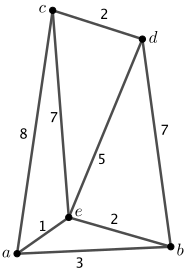
\includegraphics[width=\linewidth]{external/Graph_metric.pdf}
\end{image}%
\tcblower
\end{figureptx}%
\begin{enumerate}[font=\bfseries,label=(\alph*),ref=\alph*]%
\item{}Determine all of the open balls \(B(a,\delta)\) for every positive real number \(\delta\).%
\item{}Find all of the neighborhoods of \(a\).%
\end{enumerate}%
\end{divisionexercise}%
\begin{divisionexercise}{5}{}{}{exercise-ex_linear_continuous1}%
\begin{enumerate}[font=\bfseries,label=(\alph*),ref=\alph*]%
\item{}Let \(f: (\R,d_E) \to (\R,d_E)\) be defined by \(f(x) = ax+b\) for some real numbers \(a\) and \(b\) with \(a \neq 0\). Let \(p \in \R\) and let \(r \gt 0\). Show that \(f^{-1}(B(f(p),r))\) contains an open ball centered at \(p\). Conclude that every linear function from \((\R,d_E)\) to \((\R,d_E)\) is continuous.%
\par\smallskip%
\noindent\textbf{\blocktitlefont Hint}.\hypertarget{hint-ex_linear_continuous1-a-b}{}\quad{}By \hyperlink{exercise-ex_sum_continuous}{Exercise~{\xreffont 5}} we can assume \(a \gt 0\) to simplify the problem.%
\item{}Let \(f: (\R,d_E) \to (\R,d_E)\) be defined by \(f(x) = ax^2+bx+c\) for some real numbers \(a\), \(b\), and \(c\) with \(a \neq 0\). Let \(p \in \R\) and let \(r \gt 0\). \(f^{-1}(B(f(p),r))\) contains an open ball centered at \(p\). Conclude that every quadratic function from \((\R,d_E)\) to \((\R,d_E)\) is continuous.%
\par\smallskip%
\noindent\textbf{\blocktitlefont Hint}.\hypertarget{hint-ex_linear_continuous1-b-b}{}\quad{}Consider cases.%
\end{enumerate}%
\end{divisionexercise}%
\begin{divisionexercise}{6}{}{}{exercise-ex_metric_continuous}%
Let \((X,d)\) be a metric space, and let \(A\) be a nonempty subset of \(X\). \hyperlink{exercise-ex_GLB_triangle}{Exercise~{\xreffont 11}} tells us that%
\begin{equation*}
d(b,A) \leq d(b,c) + d(c,A)
\end{equation*}
for all \(b, c \in X\). Define \(f: X \to \R\) by \(f(x) = d(x,A)\). Let \(b \in X\). Given \(\epsilon \gt 0\), show that there is a neighborhood \(N\) of \(b\) such that \(x \in N\) implies \(f(x) \in B(f(b),\epsilon)\). Conclude that \(f\) is a continuous function. (Assume the metric on \(\R\) is the Euclidean metric.)%
\end{divisionexercise}%
\begin{divisionexercise}{7}{}{}{exercise-sec_open_balls_exer-g}%
Let \(a\) and \(b\) be distinct points of a metric space \(X\). Prove that there are neighborhoods \(N_a\) and \(N_b\) of \(a\) and \(b\) respectively such that \(N_a \cap N_b = \emptyset\).%
\end{divisionexercise}%
\begin{divisionexercise}{8}{}{}{exercise-ex_Nghb_properties}%
Let \((X,d)\) be a metric space and let \(a \in X\). Prove each of the following.%
\begin{enumerate}[font=\bfseries,label=(\alph*),ref=\alph*]%
\item{}There is a neighborhood that contains \(a\).%
\item{}If \(N\) is a neighborhood of \(a\) and \(N \subseteq M\), then \(M\) is a neighborhood of \(a\).%
\item{}If \(M\) and \(N\) are neighborhoods of \(a\), then so is \(M \cap N\).%
\end{enumerate}%
\end{divisionexercise}%
\begin{divisionexercise}{9}{}{}{exercise-sec_open_balls_exer-i}%
Let \(f: (\R,d_E) \to (\R,d_E)\) be a continuous function. Show that if \(f(a) \gt 0\) for some \(a \in \R\), then there is a neighborhood \(N\) of \(a\) such that \(f(x) \gt 0\) for all \(x \in N\).%
\end{divisionexercise}%
\begin{divisionexercise}{10}{}{}{exercise-sec_open_balls_exer-j}%
Let \((X,d)\) be a metric space where \(d\) is the discrete metric. Show that every subset of \(X\) is a neighborhood of each of its points.%
\end{divisionexercise}%
\begin{divisionexercise}{11}{}{}{exercise-sec_open_balls_exer-k}%
For each of the following, answer true if the statement is always true. If the statement is only sometimes true or never true, answer false and provide a concrete example to illustrate that the statement is false. If a statement is true, explain why.%
\begin{enumerate}[font=\bfseries,label=(\alph*),ref=\alph*]%
\item{}If \(N\) is a neighborhood of a point \(a\) in a metric space \(X\), then any open ball contained in \(N\) is also a neighborhood of \(a\).%
\item{}If \(N\) is a neighborhood of a point \(a\) in a metric space \(X\), then \(N\) is a neighborhood of each of its points.%
\item{}If \(X\) and \(Y\) are metric spaces and \(f : X \to Y\) is a continuous function, then \(f(N)\) is a neighborhood of \(f(a)\) in \(Y\) whenever \(N\) is a neighborhood of \(a\) in \(X\).%
\item{}If \(X\) and \(Y\) are metric spaces and \(f : X \to Y\) is continuous at \(a \in X\), and \(N\) is a neighborhood of \(f(a)\) in \(Y\), then \(f^{-1}(N)\) is a neighborhood of \(a\) in \(X\).%
\item{}If \(a\) is a point in a metric space \(X\) and if \(\delta\) is a positive real number, then the open ball \(B(a,\delta)\) contains infinitely many points of \(X\).%
\item{}If \(N_1\), \(N_2\), \(\ldots\), \(N_k\) are neighborhoods of a point \(a\) in a metric space \(X\) for some positive integer \(k\), then \(\bigcap_{i=1}^k N_i\) is a neighborhood of \(a\).%
\item{}If \(N_{\alpha}\) is a neighborhood of a point \(a\) in a metric space \(X\) for all \(\alpha\) in some indexing set \(I\), then \(\bigcap_{\alpha \in I} N_{\alpha}\) is a neighborhood of \(a\).%
\end{enumerate}%
\end{divisionexercise}%
\end{exercises-section}
\end{chapterptx}
 %
%
\typeout{************************************************}
\typeout{Chapter 8 Open Sets in Metric Spaces}
\typeout{************************************************}
%
\begin{chapterptx}{Chapter}{Open Sets in Metric Spaces}{}{Open Sets in Metric Spaces}{}{}{chapter-chap_open_sets}
\renewcommand*{\chaptername}{Chapter}
\begin{objectives}{Focus Questions}{objectives-chap_open_sets-b}
%
\begin{itemize}[label=\textbullet]
\item{}What is an open set in a metric space?%
\item{}What is an interior point of a subset of a metric space? How are interior points related to open sets?%
\item{}What is the interior of a set? How is the interior of a set related to open sets?%
\item{}How can we use open sets to determine the continuity of a function?%
\item{}What important properties do open sets have in relation to unions and intersections?%
\end{itemize}
\end{objectives}
%
%
\typeout{************************************************}
\typeout{Section  Introduction}
\typeout{************************************************}
%
\begin{sectionptx}{Section}{Introduction}{}{Introduction}{}{}{section-sec_open_sets_intro}
Consider the interval \((a,b)\) in \(\R\) using the Euclidean metric. If \(m = \frac{a+b}{2}\), then \((a,b) = B\left(m,\frac{b-a}{2}\right)\), so every open interval is an open ball. As an open ball, an open interval \((a,b)\) is a neighborhood of each of its points. This is the foundation for the definition of an open set in a metric space.%
\par
Recall that we defined a subset \(N\) of \(X\) to be neighborhood of point \(a\) in a metric space \((X,d)\) if \(N\) contains an open ball \(B(a, \epsilon)\) for some \(\epsilon \gt 0\). We saw that every open ball is a neighborhood of each of its points, and we will now extend that idea to define an \terminology{open set} in a metric space.%
\begin{definition}{Definition}{}{definition-sec_open_sets_intro-d}%
A subset \(O\) of a metric space \(X\) is an open set\index{open set in a metric space} if \(O\) is a neighborhood of each of its points.%
\end{definition}
So, by definition, any open ball is an open set. Also by definition, open sets are neighborhoods of each of their points. Open sets are different than non-open sets. For example, \((0,1)\) is an open set in \(\R\) using the Euclidean metric, but \([0,1)\) is not. The reason \([0,1)\) is not an open set is that there is no open ball centered at \(0\) that is entirely contained in \([0,1)\). So \(0\) has a different property than the other points in \([0,1)\). The set \([0,1)\) is a neighborhood of each of the points in \((0,1)\), but is not a neighborhood of \(0\). We can think of the points in \((0,1)\) as being in the interior of the set \([0,1)\). This leads to the next definition.%
\begin{definition}{Definition}{}{definition-sec_open_sets_intro-f}%
\index{interior point in a subset of a metric space}%
Let \(A\) be a subset of a metric space \(X\). A point \(a \in A\) is an \terminology{interior point} of \(A\) if \(A\) is a neighborhood of \(a\).%
\end{definition}
As we will soon see, open sets can be characterized in terms of interior points.%
\begin{exploration}{Preview Activity}{}{exploration-sec_open_sets_intro-h}%
\begin{enumerate}[font=\bfseries,label=(\alph*),ref=\alph*]%
\item{}Determine if the set \(A\) is an open set in the metric space \((X,d)\). Explain your reasoning.%
\begin{enumerate}[font=\bfseries,label=(\roman*),ref=\theenumi.\roman*]%
\item{}\(X = \R\), \(d = d_E\), the Euclidean metric, \(A = [0,0.5)\).%
\item{}\(X = \{x \in \R \mid 0 \leq x \leq 1\}\), \(d = d_E\), the Euclidean metric, \(A = [0,0.5)\). Assume that the Euclidean metric is a metric on \(X\).%
\item{}\(X = \{a,b,c,d\}\), \(d\) is the discrete metric defined by%
\begin{equation*}
d(x,y) = \begin{cases}0 \amp \text{ if }  x = y \\ 1 \amp \text{ if }  x \neq y, \end{cases}
\end{equation*}
and \(A = \{a,b\}\).%
\end{enumerate}%
\item{}\begin{enumerate}[font=\bfseries,label=(\roman*),ref=\theenumi.\roman*]%
\item{}What are the interior points of the following sets in \((\R, d_E)\)? Explain.%
\begin{equation*}
(0,1) \ \ \ (0,1] \ \ \ [0,1) \ \ \ [0,1]\text{.}
\end{equation*}
%
\item{}Let \(A = \{0, 1, 2\}\) in \((\R, d_E)\). What are the interior points of \(A\)? Explain.%
\item{}Let \(\Q\) be the set of rational numbers in \((\R, d_E)\). What are the interior points of \(\Q\)? Explain.%
\end{enumerate}%
\end{enumerate}%
\end{exploration}%
\end{sectionptx}
%
%
\typeout{************************************************}
\typeout{Section  Open Sets}
\typeout{************************************************}
%
\begin{sectionptx}{Section}{Open Sets}{}{Open Sets}{}{}{section-sec_open_sets}
Open sets are vitally important in topology. In fact, we will see later that every topological space is completely defined by its open sets. Recall that an open ball is an open set. There are other subsets that every metric space contains, and we might ask if they are open or not.%
\begin{activity}{Activity}{}{activity-sec_open_sets-c}%
Let \(X\) be a metric space.%
\begin{enumerate}[font=\bfseries,label=(\alph*),ref=\alph*]%
\item{}Is \(\emptyset\) an open set in \(X\)? Explain.%
\item{}Is \(X\) an open set in \(X\)? Explain.%
\end{enumerate}%
\end{activity}%
We have defined open balls, and open balls are the canonical examples of open sets. In fact, as the following theorem shows, the open balls determine the open sets.%
\begin{theorem}{Theorem}{}{}{theorem-thm_OS_1}%
Let \(X\) be a metric space. A subset \(O\) of \(X\) is open if and only if \(O\) is a union of open balls.%
\end{theorem}
\begin{proof}{Proof}{}{proof-thm_OS_1-b}
Let \(X\) be a metric space and \(O\) a subset of \(X\). To prove this biconditional statement we first assume that \(O\) is an open set and demonstrate that \(O\) is a union of open balls. Let \(a \in O\). Since \(O\) is open, there exists \(\epsilon_a \gt 0\) so that \(B(a, \epsilon_a) \subseteq O\). We will show that%
\begin{equation*}
O = \bigcup_{a \in O} B(a, \epsilon_a)\text{.}
\end{equation*}
%
\par
By the way we chose \(\epsilon_a\), \(B(a, \epsilon_a) \subseteq O\) for every \(a \in O\). So \(\bigcup_{a \in O} B(a, \epsilon_a) \subseteq O\). For the reverse containment, let \(x \in O\). Then \(x \in B(x, \epsilon_x)\) and so \(x \in \bigcup_{a \in O} B(a, \epsilon_a)\). Thus, \(O \subseteq \bigcup_{a \in O} B(a, \epsilon_a)\). We conclude that \(O\) is a union of open balls if \(O\) is an open set.%
\par
The proof of the converse is left for the following activity.%
\end{proof}
\begin{activity}{Activity}{}{activity-sec_open_sets-f}%
Let \(X\) be a metric space. To prove the remaining implication of \hyperref[theorem-thm_OS_1]{Theorem~{\xreffont\ref{theorem-thm_OS_1}}}, assume that a subset \(O\) of \(X\) is a union of open balls.%
\begin{enumerate}[font=\bfseries,label=(\alph*),ref=\alph*]%
\item{}What do we need to show to prove that \(O\) is an open set?%
\item{}Let \(x \in O\). Why is there an open ball \(B\) in \(O\) that contains \(x\)?%
\item{}Complete the proof to show that \(O\) is an open set.%
\end{enumerate}%
\end{activity}%
\hyperref[theorem-thm_OS_1]{Theorem~{\xreffont\ref{theorem-thm_OS_1}}} tells us that every open set is made up of open balls, so the open balls generate all open sets much like a basis of a vector space in linear algebra generates all of the elements of the vector space. For this reason we call the set of open balls in a metric space a \terminology{basis} for the open sets of the metric space. We will discuss this idea in more detail in a subsequent section.%
\end{sectionptx}
%
%
\typeout{************************************************}
\typeout{Section  Unions and Intersections of Open Sets}
\typeout{************************************************}
%
\begin{sectionptx}{Section}{Unions and Intersections of Open Sets}{}{Unions and Intersections of Open Sets}{}{}{section-sec_union_int_open_sets}
Once we have defined open sets we might wonder about what happens if we take a union or intersection of open sets.%
\begin{activity}{Activity}{}{activity-act_Open_union}%
\begin{enumerate}[font=\bfseries,label=(\alph*),ref=\alph*]%
\item{}Let \(A = (-2,1)\) and \(B = (-1,2)\) in \((\R, d_E)\).%
\begin{enumerate}[font=\bfseries,label=(\roman*),ref=\theenumi.\roman*]%
\item{}Is \(A \cup B\) open? Explain.%
\item{}Is \(A \cap B\) open? Explain.%
\end{enumerate}%
\item{}Let \(X = \R\) with the Euclidean metric. Let \(A_n = \left(1-\frac{1}{n}, 1+\frac{1}{n}\right)\) for each \(n \in \Z^+\).%
\begin{enumerate}[font=\bfseries,label=(\roman*),ref=\theenumi.\roman*]%
\item{}What is \(\bigcup_{n \geq 1} A_n\)? A proof is not necessary.%
\item{}Is \(\bigcup_{n \geq 1} A_n\) open in \(\R\)? Explain.%
\item{}What is \(\bigcap_{n \geq 1} A_n\)? A proof is not necessary.%
\item{}Is \(\bigcap_{n \geq 1} A_n\) open in \(\R\)? Explain.%
\end{enumerate}%
\end{enumerate}%
\end{activity}%
\hyperref[activity-act_Open_union]{Activity~{\xreffont\ref{activity-act_Open_union}}} demonstrates that an arbitrary intersection of open sets is not necessarily open. However, there are some things we can say about unions and intersections of open sets.%
\begin{theorem}{Theorem}{}{}{theorem-sec_union_int_open_sets-e}%
Let \(X\) be a metric space.%
\begin{enumerate}
\item{}Any union of open sets in \(X\) is an open set in \(X\).%
\item{}Any finite intersection of open sets in \(X\) is an open set in \(X\).%
\end{enumerate}
%
\end{theorem}
\begin{proof}{Proof}{}{proof-sec_union_int_open_sets-e-b}
Let \(X\) be a metric space. To prove part 1, assume that \(\{O_{\alpha}\}\) is a collection of open sets in \(X\) for \(\alpha\) in some indexing set \(I\) and let \(O = \bigcup_{\alpha \in I} O_{\alpha}\). By \hyperref[theorem-thm_OS_1]{Theorem~{\xreffont\ref{theorem-thm_OS_1}}}, we know that \(O_{\alpha}\) is a union of open balls for each \(\alpha \in I\). Combining all of these open balls together shows that \(O\) is a union of open balls and is therefore an open set by \hyperref[theorem-thm_OS_1]{Theorem~{\xreffont\ref{theorem-thm_OS_1}}}.%
\par
For part 2, assume that \(O_1\), \(O_2\), \(\ldots\), \(O_n\) are open sets in \(X\) for some \(n \in \Z^+\). To show that \(O = \bigcap_{k=1}^n O_k\) is an open set, we will show that \(O\) is a neighborhood of each of its points. Let \(x \in O\). Then \(x \in O_k\) for each \(1 \leq k \leq n\). Let \(k\) be between 1 and \(n\). Since \(O_k\) is open, we know that \(O_k\) is a neighborhood of each of its points. So there exists \(\epsilon_k \gt 0\) such that \(B(x, \epsilon_k) \subseteq O_k\). Since there are only finitely many values of \(k\), let \(\epsilon = \min\{\epsilon_k \mid 1 \leq k \leq n\}\). Then \(B(x, \epsilon) \subseteq B(x, \epsilon_k)\) for each \(k\) and so \(B(x, \epsilon) \subseteq \bigcap_{k=1}^n O_k = O\). Therefore, \(O\) is a neighborhood of each of its points and \(O\) is an open set.%
\end{proof}
\end{sectionptx}
%
%
\typeout{************************************************}
\typeout{Section  Continuity and Open Sets}
\typeout{************************************************}
%
\begin{sectionptx}{Section}{Continuity and Open Sets}{}{Continuity and Open Sets}{}{}{section-sec_cont_open_sets}
Recall that we showed that a function \(f\) from a metric space \((X,d_X)\) to a metric space \((Y,d_Y)\) is continuous if and only if \(f^{-1}(N)\) is a neighborhood of \(a \in X\) whenever \(N\) is a neighborhood of \(f(a)\) in \(Y\). We can now provide another characterization of continuous functions in terms of open sets. This is the characterization that will serve as our definition of continuity in topological spaces.%
\begin{theorem}{Theorem}{}{}{theorem-thm_Open_continuity}%
Let \(f\) be a function from a metric space \((X,d_X)\) to a metric space \((Y,d_Y)\). Then \(f\) is continuous if and only if \(f^{-1}(O)\) is an open set in \(X\) whenever \(O\) is an open set in \(Y\).%
\end{theorem}
\begin{proof}{Proof}{}{proof-thm_Open_continuity-b}
Let \((X, d_X)\) and \((Y,d_Y)\) be metric spaces, and let \(f : X \to Y\) be a function. To prove this biconditional statement we need to prove both implications. First assume that \(f\) is a continuous function. We must show that \(f^{-1}(O)\) is an open set in \(X\) for every open set \(O\) in \(Y\). So let \(O\) be an open set in \(Y\). To demonstrate that \(f^{-1}(O)\) is open in \(X\), we will show that \(f^{-1}(O)\) is a neighborhood of each of its points. Let \(a \in f^{-1}(O)\). Then \(f(a) \in O\). Now \(O\) is an open set, so there is an open ball \(B(f(a), \epsilon)\) around \(f(a)\) that is entirely contained in \(O\). Since \(B(f(a), \epsilon)\) is a neighborhood of \(f(a)\), we know that \(f^{-1}(B(f(a), \epsilon))\) is a neighborhood of \(a\). Thus, there exists \(\delta \gt 0\) so that \(B(a, \delta) \subseteq f^{-1}(B(f(a), \epsilon))\). Now \(f(B(a, \delta)) \subseteq B(f(a), \epsilon) \subseteq O\), and so \(B(a, \delta) \subseteq f^{-1}(O)\). We conclude that \(f^{-1}(O)\) is a neighborhood of each of its points and is therefore an open set in \(X\).%
\par
The proof of the reverse implication is left for the next activity.%
\end{proof}
\begin{activity}{Activity}{}{activity-sec_cont_open_sets-d}%
Let \(f\) be a function from a metric space \((X,d_X)\) to a metric space \((Y,d_Y)\).%
\begin{enumerate}[font=\bfseries,label=(\alph*),ref=\alph*]%
\item{}What assumption do we make to prove the remaining implication of \hyperref[theorem-thm_Open_continuity]{Theorem~{\xreffont\ref{theorem-thm_Open_continuity}}}? What do we need to demonstrate to prove the conclusion?%
\item{}Let \(a \in X\), and let \(N\) be a neighborhood of \(f(a)\) in \(Y\). Why does there exist an \(\epsilon \gt 0\) so that \(B(f(a), \epsilon) \subseteq N\).%
\item{}What does our hypothesis tell us about \(f^{-1}(B(f(a), \epsilon))\) in \(X\)?%
\item{}Why is \(f^{-1}(N)\) a neighborhood of \(a\)? How does this show that \(f\) is a continuous function?%
\end{enumerate}%
\end{activity}%
Recall that every open set is a union of open balls, so we can simplify proofs of continuous functions in metric spaces by working only with open balls instead of arbitrary open sets. The next activity provides the details.%
\begin{activity}{Activity}{}{activity-act_continuity_balls}%
In this activity we prove the following corollary to \hyperref[theorem-thm_Open_continuity]{Theorem~{\xreffont\ref{theorem-thm_Open_continuity}}}.%
\begin{corollary}{Corollary}{}{}{corollary-cor_continuity_balls}%
A function \(f\) from a metric space \((X,d_X)\) to a metric space \((Y,d_Y)\) is continuous if and only if \(f^{-1}(B)\) is open in \(X\) whenever \(B\) is an open ball in \(Y\).%
\end{corollary}
To set up the proof, let \((X,d_X)\) and \((Y,d_Y)\) be metric spaces, and let \(f: X \to Y\) be a function.%
\begin{enumerate}[font=\bfseries,label=(\alph*),ref=\alph*]%
\item{}Since the corollary is a biconditional statement, we need to prove both implications. First, assume that \(f\) is continuous. Use \hyperref[theorem-thm_Open_continuity]{Theorem~{\xreffont\ref{theorem-thm_Open_continuity}}} to explain why \(f^{-1}(B)\) is open in \(X\) whenever \(B\) is an open ball in \(Y\).%
\item{}For the remaining implication, assume that \(f^{-1}(B)\) is an open set in \(X\) for any open ball \(B\) in \(Y\). To show that \(f\) is a continuous function, we will use \hyperref[theorem-thm_Open_continuity]{Theorem~{\xreffont\ref{theorem-thm_Open_continuity}}} and show that \(f^{-1}(O)\) is open in \(X\) whenever \(O\) is an open set in \(Y\). So let \(O\) be an open set in \(Y\).%
\begin{enumerate}[font=\bfseries,label=(\roman*),ref=\theenumi.\roman*]%
\item{}What does \hyperref[theorem-thm_OS_1]{Theorem~{\xreffont\ref{theorem-thm_OS_1}}} tell us about \(O\).%
\item{}Recall that \hyperref[lemma-lem_functions_subsets]{Lemma~{\xreffont\ref{lemma-lem_functions_subsets}}} tells us that if \(\{B_{\beta}\}\) is a collection of subsets of \(Y\) for \(\beta\) in some indexing set \(J\), then%
\begin{equation*}
f^{-1}\left(\bigcup_{\beta \in J} B_{\beta}\right) = \bigcup_{\beta \in J} f^{-1}(B_{\beta})\text{.}
\end{equation*}
Use \hyperref[lemma-lem_functions_subsets]{Lemma~{\xreffont\ref{lemma-lem_functions_subsets}}} to show that \(f^{-1}(O)\) is open in \(X\) and conclude that \(f\) is a continuous function.%
\end{enumerate}%
\end{enumerate}%
\end{activity}%
\begin{example}{Example}{}{example-exp_linear_continuous}%
As an example of \hyperref[corollary-cor_continuity_balls]{Corollary~{\xreffont\ref{corollary-cor_continuity_balls}}}, we prove that the square function from \(\R\) to \(\R\) is a continuous function. Let \(X = \R\) with the Euclidean metric \(d_E\), and let \(f: X \to X\) be defined by \(f(x) = x^2\). We will show that \(f\) is a continuous function by verifying that \(f^{-1}(B)\) is open in \(X\) for every open ball \(B\) in \(X\). Let \(B = B(b,\beta) = (b-\beta,
b+\beta)\) be an open ball in \(X\). Let \(B' = B(b,\beta) \cap (\R^+ \cup \{0\})\). We consider cases.%
\begin{itemize}[label=\textbullet]
\item{}Suppose that \(B' = \emptyset\). Then \(f^{-1}(B) = \emptyset\) and \(f^{-1}(B)\) is open in \(X\).%
\item{}Suppose that \(B' = [0, b+\beta)\). Then \(f^{-1}(B) = (-\sqrt{b+\beta}, \sqrt{b+\beta})\) and \(f^{-1}(B)\) is open in \(X\).%
\item{}The final case is \(B' = (b-\beta, b+\beta)\). Then%
\begin{equation*}
f^{-1}(B) = (-\sqrt{b+\beta}, -\sqrt{b-\beta}) \cup (\sqrt{b-\beta}, \sqrt{b+\beta})
\end{equation*}
and \(f^{-1}(B)\) is open in \(X\).%
\end{itemize}
%
\par
Since the inverse image of every open ball is an open set, we conclude that \(f\) is a continuous function.%
\end{example}
\end{sectionptx}
%
%
\typeout{************************************************}
\typeout{Section  The Interior of a Set}
\typeout{************************************************}
%
\begin{sectionptx}{Section}{The Interior of a Set}{}{The Interior of a Set}{}{}{section-sec_interior_set}
Open sets can be characterized in terms of their interior points. By definition, every open set is a neighborhood of each of its points, so every point of an open set \(O\) is an interior point of \(O\). Conversely, if every point of a set \(O\) is an interior point, then \(O\) is a neighborhood of each of its points and is open. This argument is summarized in the next theorem.%
\begin{theorem}{Theorem}{}{}{theorem-sec_interior_set-c}%
Let \(X\) be a metric space. A subset \(O\) of \(X\) is open if and only if every point of \(O\) is an interior point of \(O\).%
\end{theorem}
The collection of interior points in a set form a subset of that set, called the \terminology{interior} of the set.%
\begin{definition}{Definition}{}{definition-sec_interior_set-e}%
The interior \index{interior of a set} of a subset \(A\) of a metric space \(X\) is the set%
\begin{equation*}
\Int(A) = \{a \in A \mid a \text{ is an interior point of }  A\}\text{.}
\end{equation*}
%
\end{definition}
\begin{activity}{Activity}{}{activity-sec_interior_set-f}%
Determine \(\Int(A)\) for each of the sets \(A\).%
\begin{enumerate}[font=\bfseries,label=(\alph*),ref=\alph*]%
\item{}\(A = (0,1]\) in \((\R, d_E)\)%
\item{}\(A = [0,1]\) in \((\R, d_E)\)%
\item{}\(A = \{-2\} \cup [0,5] \cup \{7,8,9\}\) in \((\R,d_E)\)%
\end{enumerate}%
\end{activity}%
One might expect that the interior of a set is an open set. This is true, but we can say even more. As \hyperref[theorem-thm_Interior_MS]{Theorem~{\xreffont\ref{theorem-thm_Interior_MS}}} will show, if \(A\) is a subset of a metric space \(X\), not only is \(\Int(A)\) an open set, but every open set that is contained in \(A\) is a subset of \(\Int(A)\). So \(\Int(A)\) is the largest, in the sense of containment, open subset of \(X\) that contains \(A\).%
\begin{theorem}{Theorem}{}{}{theorem-thm_Interior_MS}%
Let \((X,d)\) be a metric space, and let \(A\) be a subset of \(X\). Then interior of \(A\) is the largest open subset of \(X\) contained in \(A\).%
\end{theorem}
\begin{proof}{Proof}{}{proof-thm_Interior_MS-b}
Let \((X,d)\) be a metric space, and let \(A\) be a subset of \(X\). We need to prove that \(\Int(A)\) is an open set in \(X\), and that \(\Int(A)\) is the largest open subset of \(X\) contained in \(A\). First we demonstrate that \(\Int(A)\) is an open set. Let \(a \in \Int(A)\). Then \(a\) is an interior point of \(A\), so \(A\) is a neighborhood of \(a\). This implies that there exists an \(\epsilon \gt 0\) so that \(B(a, \epsilon) \subseteq A\). But \(B(a, \epsilon)\) is a neighborhood of each of its points, so every point in \(B(a, \epsilon)\) is an interior point of \(A\). It follows that \(B(a, \epsilon) \subseteq \Int(A)\). Thus, \(\Int(A)\) is a neighborhood of each of its points and, consequently, \(\Int(A)\) is an open set.%
\par
The proof that \(\Int(A)\) is the largest open subset of \(X\) contained in \(A\) is left for the next activity.%
\end{proof}
\begin{activity}{Activity}{}{activity-sec_interior_set-i}%
Let \((X,d)\) be a metric space, and let \(A\) be a subset of \(X\).%
\begin{enumerate}[font=\bfseries,label=(\alph*),ref=\alph*]%
\item{}What will we have to show to prove that \(\Int(A)\) is the largest open subset of \(X\) contained in \(A\)?%
\item{}Suppose that \(O\) is an open subset of \(X\) that is contained in \(A\), and let \(x \in O\). What does the fact that \(O\) is open tell us?%
\item{}Complete the proof that \(O \subseteq \Int(A)\).%
\end{enumerate}%
\end{activity}%
One consequence of \hyperref[theorem-thm_Interior_MS]{Theorem~{\xreffont\ref{theorem-thm_Interior_MS}}} is the following.%
\begin{corollary}{Corollary}{}{}{corollary-sec_interior_set-k}%
A subset \(O\) of a metric space \(X\) is open if and only if \(O = \Int(O)\).%
\end{corollary}
The proof is left for \hyperlink{exercise-ex_O_int_O}{Exercise~{\xreffont 2}}.%
\end{sectionptx}
%
%
\typeout{************************************************}
\typeout{Section  Summary}
\typeout{************************************************}
%
\begin{sectionptx}{Section}{Summary}{}{Summary}{}{}{section-sec_open_sets_summ}
Important ideas that we discussed in this section include the following.%
\begin{itemize}[label=\textbullet]
\item{}A subset \(O\) of a metric space \((X,d)\) is an open set if \(O\) is a neighborhood of each of its points. Alternatively, \(O\) is open if \(O\) is a union of open balls.%
\item{}A point \(a\) in a subset \(A\) of a metric space \((X,d)\) is an interior point of \(A\) if \(A\) is a neighborhood of \(a\). A set \(O\) is open if every point of \(O\) is an interior point of \(O\).%
\item{}The interior of a set is the set of all interior points of the set. The interior of a set \(A\) in a metric space \(X\) is the largest open subset of \(X\) contained in \(A\). A set is open if and only if the set is equal to its interior.%
\item{}A function \(f\) from a metric space \(X\) to a metric space \(Y\) is continuous if \(f^{-1}(O)\) is open in \(X\) whenever \(O\) is open in \(Y\).%
\item{}Any union of open sets is open, while any finite intersection of open sets is open.%
\end{itemize}
%
\end{sectionptx}
%
%
\typeout{************************************************}
\typeout{Exercises  Exercises}
\typeout{************************************************}
%
\begin{exercises-section}{Exercises}{Exercises}{}{Exercises}{}{}{exercises-sec_open_sets_exer}
\begin{divisionexercise}{1}{}{}{exercise-sec_open_sets_exer-a}%
Let \(d\) be the discrete metric. Let \((X,d)\) be a metric space.%
\begin{enumerate}[font=\bfseries,label=(\alph*),ref=\alph*]%
\item{}Show that every subset of \(X\) is open.%
\item{}Let \((Y, d_Y)\) be a metric space. Prove that every function \(f: X \to Y\) is continuous.%
\item{}Is it also true that every function \(f: Y \to X\) is continuous? If yes, prove your answer. If no, find a counterexample.%
\end{enumerate}%
\end{divisionexercise}%
\begin{divisionexercise}{2}{}{}{exercise-ex_O_int_O}%
Prove that a subset \(O\) of a metric space \(X\) is open if and only if \(O = \Int(O)\).%
\end{divisionexercise}%
\begin{divisionexercise}{3}{}{}{exercise-sec_open_sets_exer-c}%
Let \(A\) and \(B\) be subsets of a metric space \(X\) with \(A \subseteq B\). Prove or disprove the following.%
\begin{enumerate}[font=\bfseries,label=(\alph*),ref=\alph*]%
\item{}\(\Int(A) \subseteq \Int(B)\)%
\item{}\(\Int(\Int(A)) = \Int(A)\)%
\end{enumerate}%
\end{divisionexercise}%
\begin{divisionexercise}{4}{}{}{exercise-sec_open_sets_exer-d}%
Let \(a, b \in \R\) with \(a \lt b\). Show that the set \((a,b]\) in \((\R, d_E)\) is not an open set.%
\end{divisionexercise}%
\begin{divisionexercise}{5}{}{}{exercise-sec_open_sets_exer-e}%
Let \(A = \{(x,y) \in \R^2 \mid 1 \lt x \lt 3, 0 \lt y \lt 1\}\).%
\begin{enumerate}[font=\bfseries,label=(\alph*),ref=\alph*]%
\item{}Is \(A\) an open set in \((\R^2, d_E)\)? Prove your answer.%
\item{}Is \(A\) an open set in \((\R^2, d_T)\)? Prove your answer.%
\item{}Is \(A\) an open set in \((\R^2, d_M)\)? Prove your answer.%
\end{enumerate}%
\end{divisionexercise}%
\begin{divisionexercise}{6}{}{}{exercise-sec_open_sets_exer-f}%
Let \(S\) be a finite set of points in \(\R^2\). Is the set \(\R^2 \setminus A\) an open set in \((\R^2, d_E)\)? Prove your answer.%
\end{divisionexercise}%
\begin{divisionexercise}{7}{}{}{exercise-sec_open_sets_exer-g}%
Let \((X, d_X)\) and \((Y, d_Y)\) be metric spaces and let \(f: X \to Y\) be a function. Prove that \(f\) is continuous if and only if \(f^{-1}(\Int(B)) \subseteq \Int(f^{-1}(B))\) for every subset \(B\) of \(Y\).%
\end{divisionexercise}%
\begin{divisionexercise}{8}{}{}{exercise-sec_open_sets_exer-h}%
Consider the metric space \((Q,d)\), where \(d : Q \times Q \to \R\) is defined by%
\begin{equation*}
d\left(\frac{a}{b}, \frac{u}{v}\right) = \max\{| a-u |, | b-v |\}
\end{equation*}
(The fact that \(d\) is a metric is the topic of \hyperlink{exercise-ex_MS_Q_metric}{Exercise~{\xreffont 3}}.) Describe the open ball \(B(q,2)\) in \(Q\) if \(q = \frac{2}{5}\).%
\end{divisionexercise}%
\begin{divisionexercise}{9}{}{}{exercise-sec_open_sets_exer-i}%
Let \((X,d)\) be a metric space and let \(x_1\) and \(x_2\) be distinct points in \(X\). Prove that there are open sets \(O_1\) containing \(x_1\) and \(O_2\) containing \(x_2\) such that \(O_1 \cap O_2 = \emptyset\). (This shows that we can separate points in metric spaces with open sets. Separation properties are important in topology.)%
\end{divisionexercise}%
\begin{divisionexercise}{10}{}{}{exercise-ex_linear_continuous2}%
Let \(X = \R\) with the Euclidean metric \(d_E\), and let \(Y = \R\) with the metric \(d\) defined by \(d(x,y) = \frac{|x-y|}{|x-y|+1}\) (that \(d\) is a metric is the subject of \hyperlink{exercise-ex_1_over_1_plus_t_metric}{Exercise~{\xreffont 11}}). Let \(a\) and \(b\) be real numbers and let \(f:\R \to \R\) be defined by \(f(x) = ax+b\). That is, \(f\) is an arbitrary linear function from \(\R\) to \(\R\).%
\begin{enumerate}[font=\bfseries,label=(\alph*),ref=\alph*]%
\item{}Describe the open balls in \((Y, d)\). That is, if \(a\) is a real number and \(\delta\) is a positive real number, what is the specific set of points in \(B(a, \delta)\) in \(Y\)?%
\item{}Is \(f\) from \(X\) to \(Y\) continuous for any real numbers \(a\) and \(b\)? Prove your answer.%
\item{}Is \(f\) from \(Y\) to \(X\) continuous for any real numbers \(a\) and \(b\)? Prove your answer.%
\end{enumerate}%
\end{divisionexercise}%
\begin{divisionexercise}{11}{}{}{exercise-sec_open_sets_exer-k}%
Let \(f: \R^2 \to \R\) be defined by \(f((x,y)) = x\). Assume that we use the max metric \(d_M\) on \(\R^2\) and the Euclidean metric \(d_E\) on \(\R\). Use Theorem to determine if \(f\) a continuous function. Prove your conjecture.%
\end{divisionexercise}%
\begin{divisionexercise}{12}{}{}{exercise-sec_open_sets_exer-l}%
For each of the following, answer true if the statement is always true. If the statement is only sometimes true or never true, answer false and provide a concrete example to illustrate that the statement is false. If a statement is true, explain why.%
\begin{enumerate}[font=\bfseries,label=(\alph*),ref=\alph*]%
\item{}If \(A\) and \(B\) are nonempty subsets of a metric space \(X\), then \(\Int(A \cup B) \subseteq \Int(A) \cup \Int(B)\).%
\item{}If \(A\) and \(B\) are nonempty subsets of a metric space \(X\), then \(\Int(A) \cup \Int(B) \subseteq \Int(A \cup B)\).%
\item{}If \(A\) and \(B\) are nonempty subsets of a metric space \(X\), then \(\Int(A \cap B) \subseteq \Int(A) \cap \Int(B)\).%
\item{}If \(A\) and \(B\) are nonempty subsets of a metric space \(X\), then \(\Int(A) \cap \Int(B) \subseteq \Int(A \cap B)\).%
\item{}Every subset of an open set in a metric space \((X,d)\) is open in \(X\).%
\item{}A subset \(O\) of \(\R^2\) is open under the Euclidean metric \(d_E\) if and only if \(O\) is open under the taxicab metric \(d_T\).%
\item{}Let X = \([0,1] \cup [2,3]\) endowed with the Euclidean metric. Then \([0, 1]\) is an open subset of \(X\).%
\end{enumerate}%
\end{divisionexercise}%
\end{exercises-section}
\end{chapterptx}
 %
%
\typeout{************************************************}
\typeout{Chapter 9 Sequences in Metric Spaces}
\typeout{************************************************}
%
\begin{chapterptx}{Chapter}{Sequences in Metric Spaces}{}{Sequences in Metric Spaces}{}{}{chapter-chap_sequences}
\renewcommand*{\chaptername}{Chapter}
\begin{objectives}{Focus Questions}{objectives-chap_sequences-b}
%
\begin{itemize}[label=\textbullet]
\item{}What is a sequence in a metric space?%
\item{}What does it mean for a sequence to have a limit in a metric space?%
\item{}How can we use sequences to determine the continuity of a function at a point?%
\end{itemize}
\end{objectives}
%
%
\typeout{************************************************}
\typeout{Section  Introduction}
\typeout{************************************************}
%
\begin{sectionptx}{Section}{Introduction}{}{Introduction}{}{}{section-sec_seq_intro}
We were introduced to sequences in calculus, and we can extend the notion of the limit of a sequence to metric spaces. Sequences provide an alternate way to describe many ideas in metric space. For example, we will see that we can characterize continuity in terms of sequences, and we can use sequences to determine open and closed sets.%
\par
Recall from calculus that a sequence of real numbers is a list of numbers in a specified order. We write a sequence \(a_1\), \(a_2\), \(\ldots\), \(a_n\), \(\ldots\) as \((a_n)_{n \in \Z^+}\) or just \((a_n)\). If we think of each \(a_n\) as the output of a function, we can give a more formal definition of a sequence as a function \(f: \Z^+ \to \R\), where \(a_n = f(n)\) for each \(n\).%
\par
A sequence \((a_n)\) of real numbers converges to a number \(L\) if we can make all of the numbers in the sequence as close to \(L\) as we like by choosing \(n\) to be large enough. Once again, this is an informal description that we need to make more rigorous. As we saw with continuous functions, we can make more rigorous the idea of ``closeness'' by introducing a symbol for a number that can be arbitrarily small. So we can say that the numbers \(a_n\) can get as close to a number \(L\) as we want if we can make \(| a_n - L | \lt \epsilon\) for any positive number \(\epsilon\). The idea of choosing \(n\) large enough is just finding a large enough fixed integer \(N\) so that \(| a_n - L | \lt \epsilon\) whenever \(n \geq N\). This leads to the definition.%
\begin{definition}{Definition}{}{definition-def_sequence_limit_real}%
\index{limit of a sequence of real numbers}%
A sequence \((a_n)\) of real numbers has a \terminology{limit} \(L\) if, given any \(\epsilon \gt 0\) there exists a positive integer \(N\) (depending only on \(\epsilon\)) such that%
\begin{equation*}
| a_n - L | \lt  \epsilon \ \text{ whenever }  \ n \geq N\text{.}
\end{equation*}
%
\end{definition}
When a sequence \((a_n)\) has a limit \(L\), we write%
\begin{equation*}
\lim_{n \to \infty} a_n = L\text{,}
\end{equation*}
or just \(\lim a_n = L\) (since we assume the limit for a sequence occurs as \(n\) goes to infinity) and we say that the sequence \((a_n)\) \terminology{converges} to \(L\).%
\begin{example}{Example}{}{example-sec_seq_intro-g}%
We can draw a graph of a sequence \((a_n)\) of real numbers as the set of points \((n,a_n)\). In this way we can visualize a sequence and its limit. By definition, \(L\) is a limit of the sequence \((a_n)\) if, given any \(\epsilon \gt 0\), we can go far enough out in the sequence so that the numbers in the sequence all lie in the horizontal band between \(y = L -\epsilon\) and \(L+ \epsilon\) as illustrated in \hyperref[figure-F_sequence_limit]{Figure~{\xreffont\ref{figure-F_sequence_limit}}} for the sequence \(\left(\frac{n}{1+n}\right)\).%
\begin{figureptx}{Figure}{The limit of the sequence \(\left(\frac{n}{1+n}\right)\).}{figure-F_sequence_limit}{}%
\begin{image}{0.05}{0.9}{0.05}{}%
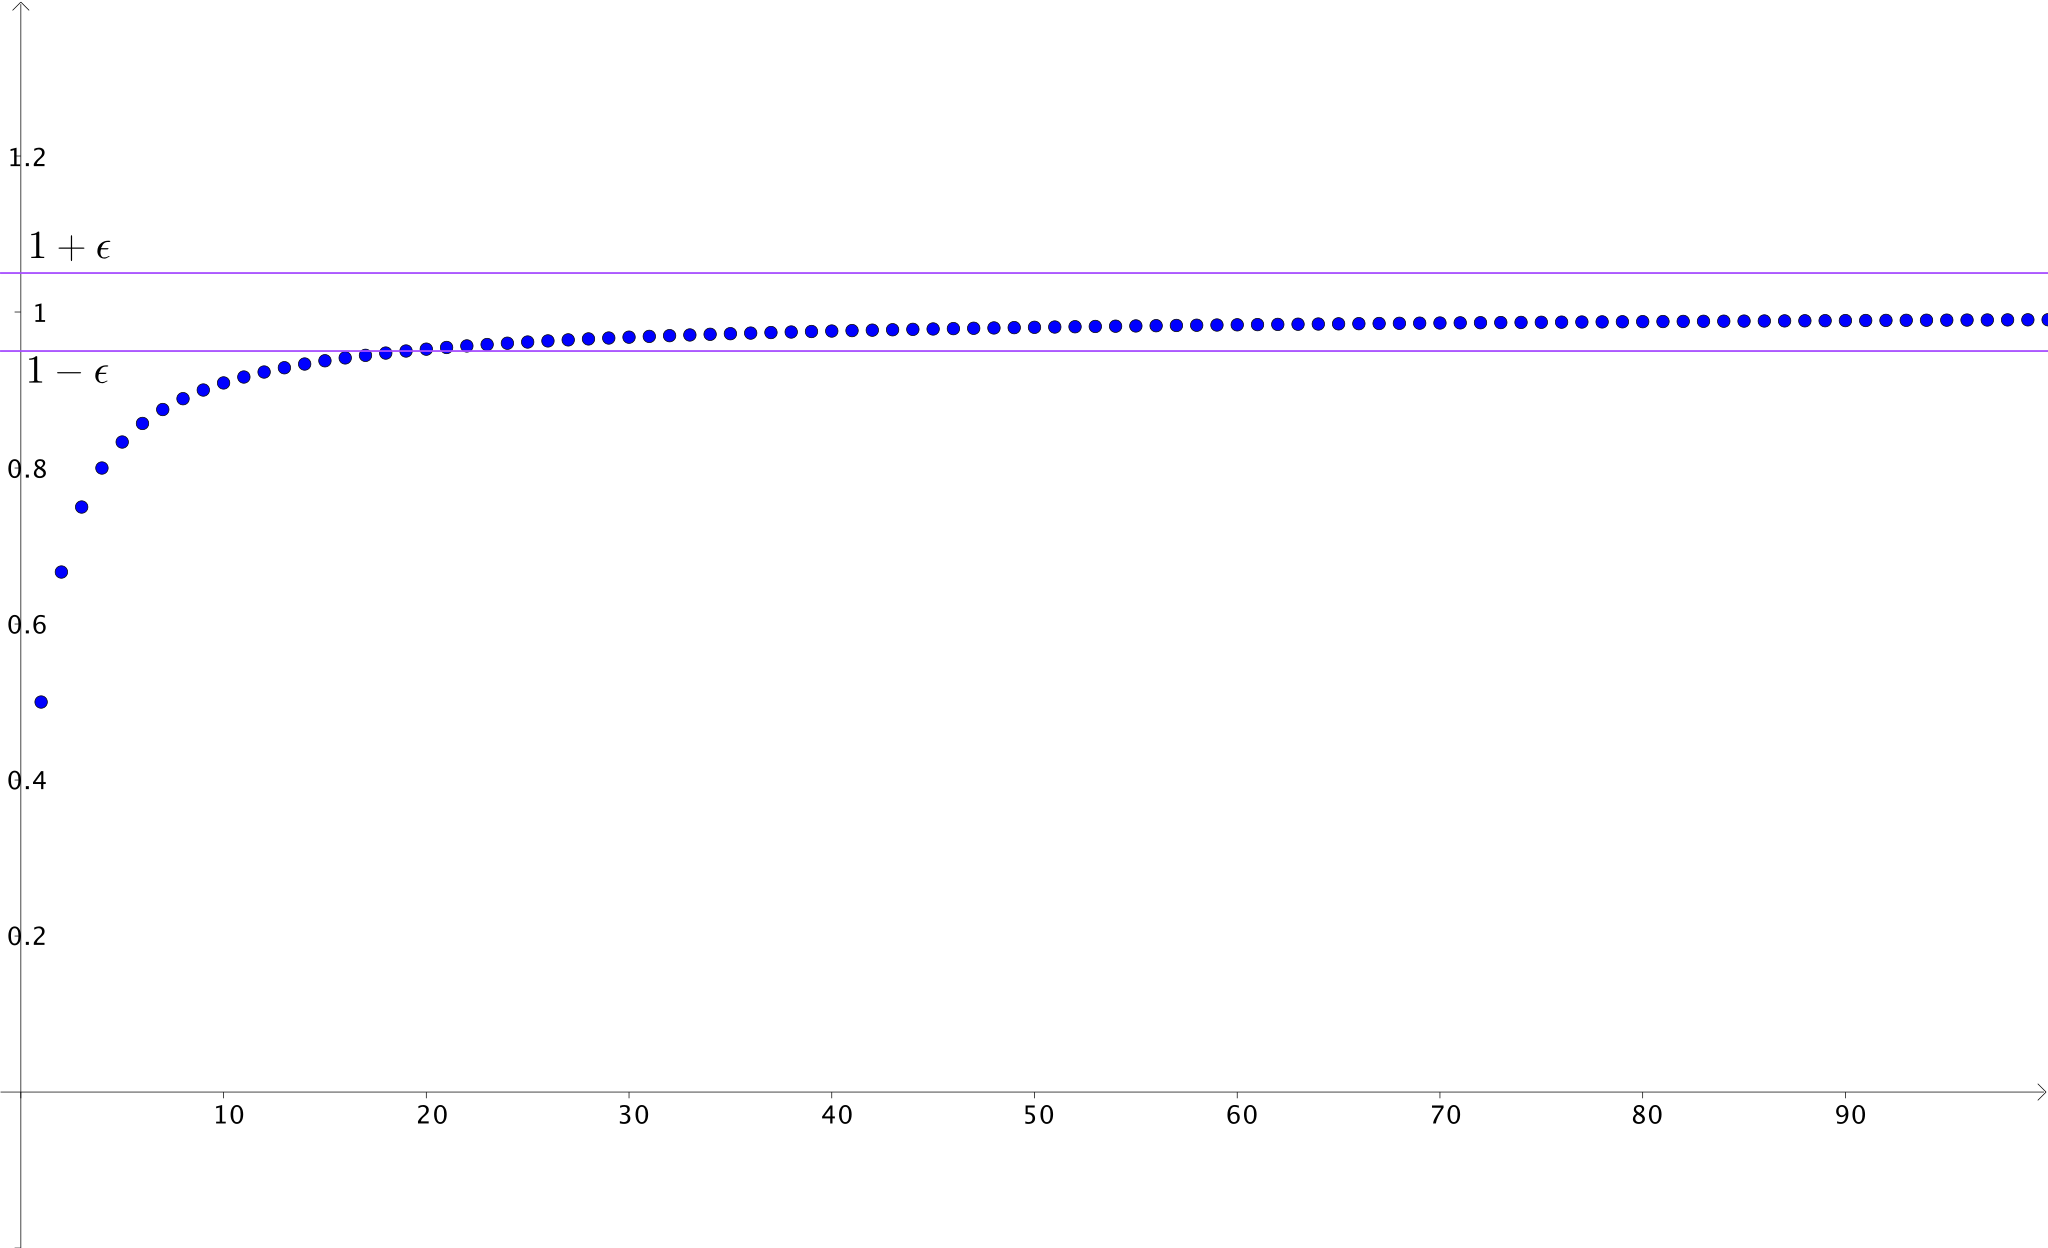
\includegraphics[width=\linewidth]{external/Sequence_limit.pdf}
\end{image}%
\tcblower
\end{figureptx}%
To verify that the limit of the sequence \(\left(\frac{n}{1+n}\right)\) is \(1\), we start with \(\epsilon \gt 0\).%
\begin{quote}%
\emph{Scratch work.} Now we need to find \(N\) so that \(n \geq N\) implies \(\left| \frac{n}{1+n} - 1 \right| \lt  \epsilon\). Just as with our continuity example, this work is not part of the proof, but shows how we go about finding the \(N\) we need. To make \(\left| \frac{n}{1+n} - 1 \right| \lt  \epsilon\) we need%
\begin{align*}
\left| \frac{n}{1+n} - 1 \right| \amp \lt  \epsilon\\
\left| \frac{n}{1+n} - \frac{1+n}{1+n}  \right| \amp \lt  \epsilon\\
\left| \frac{-1}{1+n} \right| \amp \lt  \epsilon\\
1+n \amp \gt \frac{1}{\epsilon}\\
n \amp \gt \frac{1}{\epsilon} -1\text{.}
\end{align*}
Now we use this scratch work to design our proof.%
\end{quote}
Let \(N \gt \frac{1}{\epsilon} -1\) (so that \(N\) depends on \(\epsilon\)). Then for \(n \geq N\) we have%
\begin{align*}
n \amp \gt N \gt \frac{1}{\epsilon} -1\\
1+n \amp \gt \frac{1}{\epsilon}\\
|-1| \left| \frac{1}{1+n} \right| \amp \lt  \epsilon\\
\left| \frac{-1}{1+n} \right| \amp \lt  \epsilon\\
\left| \frac{n}{1+n} - 1 \right| \amp \lt  \epsilon\\
\left| \frac{n}{1+n} - \frac{1+n}{1+n}  \right| \amp \lt  \epsilon\text{.}
\end{align*}
%
\par
So the sequence \(\left(\frac{n}{1+n}\right)\) has a limit of \(1\).%
\end{example}
\hyperref[definition-def_sequence_limit_real]{Definition~{\xreffont\ref{definition-def_sequence_limit_real}}} only applies to sequences of real numbers. Ultimately, we want to phrase the definition in a way that allows us to define limits of sequences in metric spaces and topological spaces. So we have to reformulate the definition in such a way that it does not depend on distances.%
\par
Recall that \(| x-y |\) defined a metric \(d_E\) on \(\R\), that is%
\begin{equation*}
d_E(x,y) = | x-y |\text{.}
\end{equation*}
%
\par
So we can rephrase the definition of a limit of a sequence of real numbers as follows.%
\begin{definition}{Definition}{Alternate Definition.}{definition-sec_seq_intro-k}%
A sequence \((a_n)\) of real numbers has a \terminology{limit} \(L\) if, given any \(\epsilon \gt 0\) there exists a positive integer \(N\) (depending only on \(\epsilon\)) such that%
\begin{equation*}
d_E(a_n, L) \lt  \epsilon \ \text{ whenever }  \ n \geq N\text{.}
\end{equation*}
%
\end{definition}
Once we have described a limit of a sequence in terms of a metric, then we can extend the idea into any metric space.%
\begin{definition}{Definition}{}{definition-sec_seq_intro-m}%
\index{sequence in a metric space}%
A \terminology{sequence} in a metric space \((X,d)\) is a function \(f: \Z^+ \to X\).%
\end{definition}
If \(f\) is a sequence in \(X\), we write the sequence defined by \(f\) as \((f(n))\), where \(n \in \Z^+\). We also use the notation \((a_n)\), when \(a_n = f(n)\). As long as \(X\) has a metric defined on it, we can then describe the limit of a sequence.%
\begin{definition}{Definition}{}{definition-sec_seq_intro-o}%
\index{limit of a sequence in a metric space}%
Let \((X,d)\) be a metric space. A sequence \((a_n)\) in \(X\) has a \terminology{limit} \(L \in X\) if, given any \(\epsilon \gt 0\) there exists a positive integer \(N\) (depending only on \(\epsilon\)) such that%
\begin{equation*}
d(a_n, L) \lt  \epsilon \ \text{ whenever }  \ n \geq N\text{.}
\end{equation*}
%
\end{definition}
In other words, a sequence \((a_n)\) in a metric space \((X,d)\) has a limit \(L \in X\) if \(\lim d(a_n,L) = 0\) \textemdash{} or that the sequence \(d(a_n,L)\) of real numbers has a limit of \(0\). Just as with sequences of real numbers, when a sequence \((a_n)\) has a limit \(L\), we say that the sequence \((a_n)\) \terminology{converges} to \(L\), or that \(L\) is a limit of the sequence \((a_n)\).%
\begin{exploration}{Preview Activity}{}{exploration-sec_seq_intro-q}%
\begin{enumerate}[font=\bfseries,label=(\alph*),ref=\alph*]%
\item{}Explain why the sequence \(\left(\frac{1}{n}\right)\) converges to 0 in \(\R\) using the Euclidean metric \(d_E\), where%
\begin{equation*}
d_E(a,y) = | x-y |\text{.}
\end{equation*}
%
\item{}Consider the sequence \((a_n) = \left(\left(\frac{1}{n}, \frac{1}{n+1} \right)\right)\) in \((\R^2, d_T)\), where \(d_T\) is the taxicab metric%
\begin{equation*}
d_T((x_1, x_2), (y_1, y_1)) = | x_1-y_1| + | x_2-y_2 |\text{.}
\end{equation*}
Does the sequence \((a_n)\) converge? If so, find its limit and prove that your candidate is the limit. If not, explain why.%
\item{}Let \((b_n) = \left((2n,
n^2)\right)\) in the metric space \((\R^2, d)\), where \(d\) is the discrete metric defined by%
\begin{equation*}
d(x,y) = \begin{cases}0 \amp \text{ if }  x=y \\ 1 \amp \text{ if }  x \neq y. \end{cases}
\end{equation*}
Does the sequence \((b_n)\) converge? If so, find its limit and prove that your candidate is the limit. If not, explain why.%
\end{enumerate}%
\end{exploration}%
\end{sectionptx}
%
%
\typeout{************************************************}
\typeout{Section  Sequences and Continuity in Metric Spaces}
\typeout{************************************************}
%
\begin{sectionptx}{Section}{Sequences and Continuity in Metric Spaces}{}{Sequences and Continuity in Metric Spaces}{}{}{section-sec_seq_cont_metric}
We have seen that there are different ways to characterize. For example, there is the \(\epsilon - \delta\) definition and a characterization in terms of neighborhoods. In this section we investigate sequences and limits of sequences in metric spaces, and then provide a characterization of continuous functions in terms of sequences.%
\begin{activity}{Activity}{}{activity-sec_seq_cont_metric-c}%
A reasonable question to ask is if a limit of a sequence is unique. We will answer that question in this activity. Let \((X,d)\) be a metric space and \((a_n)\) a sequence in \(X\). Assume the sequence \((a_n)\) has a limit in \(X\). To show that a limit of the sequence \((a_n)\) is unique, we need to show that if \(\lim a_n = a\) and \(\lim a_n = a'\) for some \(a,
a' \in X\), then \(a=a'\).%
\par
Suppose \(\lim a_n = a\) and \(\lim a_n = a'\) for some \(a, a' \in X\). Without much to go on it might appear that proving \(a=a'\) is a difficult task. However, if \(d(a,a') \lt \epsilon\) for any \(\epsilon \gt 0\), then it will have to be the case that \(a=a'\). So let \(\epsilon \gt 0\).%
\begin{enumerate}[font=\bfseries,label=(\alph*),ref=\alph*]%
\item{}Why must there exist a positive integer \(N\) so that \(d(a_n, a) \lt \frac{\epsilon}{2}\) for all \(n \geq N\)?%
\item{}Why must there exist a positive integer \(N'\) so that \(d(a_n, a') \lt \frac{\epsilon}{2}\) for all \(n \geq N'\)?%
\item{}Now let \(m = \max\{N, N'\}\). What can we say about \(d(a_m,a)\) and \(d(a_m,a')\)? Why?%
\item{}Use the triangle inequality to conclude that \(d(a,a') \lt \epsilon\). What else can we conclude?%
\end{enumerate}%
\end{activity}%
Now we will examine how continuity can be described in terms of sequences. The basic idea is this. Suppose that \(f : \R \to \R\) is continuous at a point \(a\). This means that \(f\) has a limit (as a continuous function) at \(a\). So if we were to take any sequence \((a_n)\) that converges to \(a\), then the continuity of \(f\) implies that \(f(a) = f(\lim a_n) = \lim f(a_n)\). That this is both a necessary condition and a sufficient condition for continuity is given in the next theorem.%
\begin{theorem}{Theorem}{}{}{theorem-thm_seq_continuity}%
Let \((X,d_X)\) and \((Y,d_Y)\) be metric spaces, and let \(a \in X\). A function \(f:X \to Y\) is continuous at \(a\) if and only if \(\lim f(a_n) = f(a)\) for any sequence \((a_n)\) in \(X\) that converges to \(a\).%
\end{theorem}
\begin{proof}{Proof}{}{proof-thm_seq_continuity-b}
Let \((X,d_X)\) and \((Y,d_Y)\) be metric spaces, let \(a \in X\), and let \(f: X \to Y\) be a function. Assume that \(f\) is continuous at \(a\). We will show that \(\lim f(a_n) = f(a)\) for any sequence \((a_n)\) in \(X\) that converges to \(a\). Let \((a_n)\) be a sequence in \(X\) that converges to \(a\) (we know such a sequence exists, namely the sequence \((a)\)). To verify that \(\lim f(a_n) = a\), let \(\epsilon \gt 0\). The fact that \(f\) is continuous at \(a\) means that there is a \(\delta \gt 0\) so that \(d_Y(f(x),
f(a)) \lt  \epsilon\) whenever \(d_X(x,a) \lt  \delta\). Since \((a_n)\) converges to \(a\), we know that there exists a positive integer \(N\) such that \(d_X(a_n, a) \lt  \delta\) whenever \(n \geq N\). This implies that%
\begin{equation*}
d_Y(f(a_n), f(a)) \lt  \epsilon \ \text{ whenever }  \ n \geq N\text{.}
\end{equation*}
%
\par
We conclude that if \(f\) is continuous at \(a\), then \(\lim f(a_n) = f(a)\) for any sequence \((a_n)\) in \(X\) that converges to \(a\).%
\par
The proof of the reverse implication is contained in the next activity.%
\end{proof}
\begin{activity}{Activity}{}{activity-sec_seq_cont_metric-f}%
Let \((X,d_X)\) and \((Y,d_Y)\) be metric spaces, let \(a \in X\), and let \(f: X \to Y\) be a function. We prove the remaining implication of \hyperref[theorem-thm_seq_continuity]{Theorem~{\xreffont\ref{theorem-thm_seq_continuity}}}, that \(f\) is continuous at \(a\) if \(\lim f(a_n) = f(a)\) for any sequence \((a_n)\) in \(X\) that converges to \(a\), in this activity.%
\begin{enumerate}[font=\bfseries,label=(\alph*),ref=\alph*]%
\item{}To have an additional assumption with which to work, let us proceed by contradiction and assume that \(f\) is not continuous at \(a\). Why can we then say that there is an \(\epsilon \gt 0\) so that there is no \(\delta \gt 0\) with the property that \(d_X(x,a) \lt \delta\) implies \(d_Y(f(x), f(a)) \lt \epsilon\)?%
\item{}To create a contradiction, we will construct a sequence \((a_n)\) that converges to \(a\) while \((f(a_n))\) does not converge to \(f(a)\).%
\begin{enumerate}[font=\bfseries,label=(\roman*),ref=\theenumi.\roman*]%
\item{}Explain why we can find a positive integer \(K\) such that \(\frac{1}{K} \lt \epsilon\).%
\item{}If \(k \gt K\), explain why there is an element \(a_k \in B\left(a, \frac{1}{k}\right)\) so that \(d_Y(f(a_k),
f(a)) \geq \epsilon\).%
\item{}For \(k \leq K\), let \(a_k\) be any element in \(B\left(a, \frac{1}{k}\right)\). Explain why \(a\) is a limit of \((a_n)\).%
\item{}Explain why \(f(a)\) is not a limit of the sequence \((f(a_n))\). What conclusion can we draw, and why?%
\end{enumerate}%
\end{enumerate}%
\end{activity}%
One way that \hyperref[theorem-thm_seq_continuity]{Theorem~{\xreffont\ref{theorem-thm_seq_continuity}}} is often used is illustrated in the next activity.%
\begin{activity}{Activity}{}{activity-act_sequence_continuity}%
Let \(f\) be the function from \(\R\) to \(\R\), both with the Euclidean metric, defined by%
\begin{equation*}
f(x) = \begin{cases}\sin\left(\frac{1}{x}\right) \amp \text{ if }  x \neq 0 \\ 0 \amp \text{ if }  x = 0. \end{cases}
\end{equation*}
%
\par
We consider the \(f\) continuity of \(f\) at \(0\) in this activity.%
\begin{enumerate}[font=\bfseries,label=(\alph*),ref=\alph*]%
\item{}Draw a graph of \(f\) on some small interval centered at \(0\). Based on the graph, do you think \(f\) has a limit at \(0\)? Explain. (There is no right answer here, just your intuition based on the graph.)%
\item{}At which inputs is \(f(x)=1\)?%
\item{}Use the result of (b) to find a sequence \((a_n)\) that converges to \(0\) for which \(f(a_n) = 1\) for every \(n\).%
\item{}What does the result of (c) tell us about the continuity of \(f\) at \(0\)?%
\end{enumerate}%
\end{activity}%
While it can sometimes be difficult to prove a fact about all sequences that converge to a point, \hyperref[activity-act_sequence_continuity]{Activity~{\xreffont\ref{activity-act_sequence_continuity}}} shows that we can use \hyperref[theorem-thm_seq_continuity]{Theorem~{\xreffont\ref{theorem-thm_seq_continuity}}} to prove that a function \(f\) is not continuous at an input \(a\) be finding just one sequence \((a_n)\) that converges to \(a\) for which \(\lim f(a_n) \neq f(a)\). We conclude this section with one final note.%
\par
\alert{IMPORTANT NOTE:} \hyperref[theorem-thm_seq_continuity]{Theorem~{\xreffont\ref{theorem-thm_seq_continuity}}} tells us that if \(f : X \to Y\) is a continuous function, then \(f\) commutes with limits. That is, if \((a_n)\) is a sequence in \(X\) that converges to \(a \in X\), then%
\begin{equation*}
f(a) = f(\lim a_n) = \lim f(a_n)\text{.}
\end{equation*}
%
\end{sectionptx}
%
%
\typeout{************************************************}
\typeout{Section  Summary}
\typeout{************************************************}
%
\begin{sectionptx}{Section}{Summary}{}{Summary}{}{}{section-sec_seq_summ}
Important ideas that we discussed in this section include the following.%
\begin{itemize}[label=\textbullet]
\item{}A sequence in a metric space \(X\) is a function \(f : \Z^+ \to X\).%
\item{}A sequence \((a_n)\) in a metric space \((X,d)\) has a limit \(L\) in \(X\) if, given any \(\epsilon \gt 0\) there exists a positive integer \(N\) such that \(d(a_n,L) \lt \epsilon\) whenever \(n \geq N\).%
\item{}Let \(f\) be a function from a metric space \((X,d_X)\) to m metric space \((Y,d_Y)\). Then \(f\) is continuous at \(a \in X\) if and only if \(\lim f(a_n) = f(a)\) for any sequence \((a_n)\) in \(X\) that converges to \(a\).%
\end{itemize}
%
\end{sectionptx}
%
%
\typeout{************************************************}
\typeout{Exercises  Exercises}
\typeout{************************************************}
%
\begin{exercises-section}{Exercises}{Exercises}{}{Exercises}{}{}{exercises-sec_seq_exer}
\begin{divisionexercise}{1}{}{}{exercise-sec_seq_exer-a}%
Determine, with proof, the convergence or divergence of each of the following sequences in the indicated metric spaces.%
\begin{enumerate}[font=\bfseries,label=(\alph*),ref=\alph*]%
\item{}\(a_n = 1+\frac{1}{n}\) in \((\R, d_E)\)%
\item{}\(a_n = (2,n)\) in \((\R^2, d_M)\)%
\item{}\(a_n\) is the function defined by%
\begin{equation*}
a_n(x) = \frac{1}{n}x
\end{equation*}
where \(X\) is the set of real valued functions on the interval \([0,1]\) and the metric \(d\) is defined by%
\begin{equation*}
d(f,g) = \sup\{|f(x)-g(x)| \mid x \in [0,1]\}\text{.}
\end{equation*}
(See \hyperlink{exercise-ex_GLB_function_sup_metric}{Exercise~{\xreffont 4}}.)%
\end{enumerate}%
\end{divisionexercise}%
\begin{divisionexercise}{2}{}{}{exercise-sec_seq_exer-b}%
Let \(A\) be a subset of \(\R\).%
\begin{enumerate}[font=\bfseries,label=(\alph*),ref=\alph*]%
\item{}Show that if \(A\) is bounded above, then there is a sequence \((a_n)\) in \(A\) such that \(\lim a_n = \sup(A)\).%
\item{}Show that if \(A\) is bounded below, then there is a sequence \((a_n)\) in \(A\) such that \(\lim a_n = \inf(A)\).%
\item{}Are the limits from (a) or (b) necessarily in \(A\)? Explain.%
\end{enumerate}%
\end{divisionexercise}%
\begin{divisionexercise}{3}{}{}{exercise-sec_seq_exer-c}%
Let \((X,d)\) be a metric space, let \(x \in X\), and let \(A\) be a nonempty subset of \(X\). Recall that the distance from \(x\) to \(A\) is%
\begin{equation*}
d(x,A) = \inf \{d(x,a) \mid a \in A\text{.}
\end{equation*}
In this exercise we see how we can view the distance between a point and a set in terms of sequences. Let \(m = d(x,A)\). We will show that there must be a sequence \((a_n)\) in \(A\) so that \(d(x,A) = \lim d(x,a_n)\).%
\begin{enumerate}[font=\bfseries,label=(\alph*),ref=\alph*]%
\item{}For each \(n \in \Z^+\), let \(B_n = B\left(x;m+\frac{1}{n}\right)\). Why must \(B_n \cap A \neq \emptyset\) for each \(n \in \Z^+\)?%
\item{}Let \(a_n \in B_n \cap A\) for each \(n\). What property does this sequence have? Explain how we have just proved the following theorem.%
\begin{theorem}{Theorem}{}{}{theorem-sec_seq_exer-c-c-a-b}%
Let \((X,d)\) be a metric space, let \(x \in X\), and let \(A\) be a nonempty subset of \(X\). Then there exists a sequence \((a_n)\) in \(A\) such that%
\begin{equation*}
\lim d(x,a_n) = d(x,A)\text{.}
\end{equation*}
%
\end{theorem}
\end{enumerate}%
\end{divisionexercise}%
\begin{divisionexercise}{4}{}{}{exercise-sec_seq_exer-d}%
\begin{enumerate}[font=\bfseries,label=(\alph*),ref=\alph*]%
\item{}Let \((Y,d')\) be a subspace of \((X,d)\). Let \(a_1\), \(a_2\), \(\ldots\) be a sequence of points in \(Y\) and let \(a \in Y\). Prove that if \(\lim_n a_n = a\) in \((Y,d')\), then \(\lim_n a_n = a\) in \((X,d)\).%
\item{}Show that the converse of part (a) is false by considering the subspace \((\Q, d_{\Q})\) (the rational numbers) of \((R,d)\). Let \(a_1\), \(a_2\), \(\ldots\) be a sequence of rational numbers such that \(\lim_n a_n = \sqrt{2}\). Prove that , given \(\epsilon \gt 0\), there is a positive integer \(N\) such that for \(n,
m \gt N\), \(|a_n - a_m | \lt \epsilon\). Does the sequence \(a_1\), \(a_2\), \(\ldots\) converge when considered to be a sequence of points in \(\Q\)?%
\end{enumerate}%
\end{divisionexercise}%
\begin{divisionexercise}{5}{}{}{exercise-ex_limit_properties}%
In this exercise we prove some standard results about limits of sequences from calculus. Let \((a_n)\) and \((b_n)\) be convergent sequences in a metric space \((\R,d_E)\).%
\begin{enumerate}[font=\bfseries,label=(\alph*),ref=\alph*]%
\item{}Show that \(\lim ka_n = k \lim a_n\) for any real number \(k\).%
\item{}Show that \(\lim (a_n + b_n) = \lim a_n + \lim b_n\).%
\item{}Show that the sequence \((a_n)\) is bounded. That is, show that there is a positive real number \(M\) such that \(|a_n| \leq M\) for all \(n \in \Z^+\).%
\item{}Show that \(\lim a_nb_n = \lim a_n \ \lim b_n\).%
\item{}If \(b_n \neq 0\) for every \(n\) and \(\lim b_n \neq 0\), show that \(\lim \frac{a_n}{b_n} = \frac{\lim a_n}{\lim b_n}\).%
\end{enumerate}%
\end{divisionexercise}%
\begin{divisionexercise}{6}{}{}{exercise-sec_seq_exer-f}%
Let \(f\) and \(g\) be continuous functions from \(\R\) to \(\R\), both with the standard Euclidean metric. Define the function \(fg\) from \(\R\) to \(\R\) by%
\begin{equation*}
(fg)(x) = f(x)g(x) \text{ for every }  x \in \R\text{.}
\end{equation*}
%
\begin{enumerate}[font=\bfseries,label=(\alph*),ref=\alph*]%
\item{}Prove that \(fg\) is a continuous function.%
\item{}Assume that \(g(x) \neq 0\) for every \(x \in \R\). Define the function \(\frac{f}{g}\) from \(\R\) to \(\R\) by \(\frac{f}{g}(x) = \frac{f(x)}{g(x)}\) for every \(x \in \R\). Use the definition of continuity to prove that \(\frac{f}{g}\) is a continuous function.%
\end{enumerate}%
\end{divisionexercise}%
\begin{divisionexercise}{7}{}{}{exercise-sec_seq_exer-g}%
Let \((c_n) = (a_n,b_n)\) be a sequence in \((\R^2, d_E)\). Show that the sequence \((c_n)\) converges to a point \((a,b)\) if and only if \((a_n)\) converges to \(a\) and \((b_n)\) converges to \(b\) in \((\R, d_E)\).%
\end{divisionexercise}%
\begin{divisionexercise}{8}{}{}{exercise-sec_seq_exer-h}%
Define \(f : (\R,d_E) \to (\R,d_E)\) by%
\begin{equation*}
f(x) = \begin{cases}0 \amp \text{ if }  x \text{ is irrational }  \\ x \amp \text{ if }  x \text{ is rational. } \end{cases}
\end{equation*}
%
\begin{enumerate}[font=\bfseries,label=(\alph*),ref=\alph*]%
\item{}Show that \(f\) is continuous at exactly one point. Assume that both copies of \(\R\) are given the Euclidean topology.%
\item{}Modify the function \(f\) to construct a new function \(g: \R \to \R\) such that \(g\) is continuous at exactly the numbers \(0\) and \(1\). Prove your result. Can you see how to extend this to construct a function \(h: \R \to \R\) that is continuous at any given finite number of points?%
\end{enumerate}%
\end{divisionexercise}%
\begin{divisionexercise}{9}{}{}{exercise-sec_seq_exer-i}%
Let \(X\) be the set of real valued functions on the interval \([0,1]\) and let \(d\) be the metric on \(X\) defined by%
\begin{equation*}
d(f,g) = \sup\{|f(x)-g(x)| \mid x \in [0,1]\}\text{.}
\end{equation*}
(See \hyperlink{exercise-ex_GLB_function_sup_metric}{Exercise~{\xreffont 4}}.)  There is a difference between the point-wise convergence of a sequence of functions and convergence in the metric space \((X,d)\) that we explore in this exercise. For each \(n \in \Z^+\), define \(f_n :[0,1] \to \R\) by \(f_n(x) = x^n\).%
\begin{enumerate}[font=\bfseries,label=(\alph*),ref=\alph*]%
\item{}Let \(0 \leq a \lt 1\). Show that the sequence \((a_n)\) where \(a_n = a^n\) converges to \(0\) in \((\R, d_E)\).%
\item{}Since the sequence \((1)\) converges to \(1\), if we look at the behavior at each point, we might think that the sequence \((f_n)\) converges to the function \(f\) defined by%
\begin{equation}
f(x) = \begin{cases} 0 \amp \text{ if }  x \neq 1 \\ 1 \amp \text{ if }  x=1. \end{cases}\label{men-eq_0_1_function}
\end{equation}
Determine if the sequence \((f_n)\) converges to \((f)\) in the metric space \((X,d)\).%
\item{}Suppose now we consider the sequence \((f_n)\) as a sequence of functions in \(C[0,1]\), the space of continuous functions from \(\R\) to \(\R\), using the metric%
\begin{equation*}
d(f,g) = \int_0^1 |f(x) - g(x)| \,dx\text{.}
\end{equation*}
(Refer to \hyperref[activity-act_MS_metrics]{Activity~{\xreffont\ref{activity-act_MS_metrics}}}.) The function in \hyperref[men-eq_0_1_function]{({\xreffont\ref{men-eq_0_1_function}})} is not a continuous function, so can't be a limit of the sequence \((f_n)\) in \(C[01]\). Determine if the sequence \((f_n)\) has a limit in \(C[0,1]\). If so, what is the limit? If not, verify that the sequence has no limit.%
\end{enumerate}%
\end{divisionexercise}%
\begin{divisionexercise}{10}{}{}{exercise-sec_seq_exer-j}%
For each of the following, answer true if the statement is always true. If the statement is only sometimes true or never true, answer false and provide a concrete example to illustrate that the statement is false. If a statement is true, explain why.%
\begin{enumerate}[font=\bfseries,label=(\alph*),ref=\alph*]%
\item{}If \((a_n)\) is a sequence in \((\R, d_E)\) with \(a_{n+1} \lt a_n\) for each \(n \in \Z^+\) and the set \(\{a_n\}\) is bounded below, then \(\inf \{a_n \mid n \in \Z^+\}\) is the limit of the sequence \((a_n)\).%
\item{}Let \(X\) be a metric space and \(A\) a nonempty subset of \(X\). If \(a \in X\) and if \(B(a,r)\) in \(X\) contains a point of \(A\) for every \(r \gt 0\), then there is a sequence in \(A\) that converges to \(a\).%
\item{}Let \(R\) be a nonempty subset of \(\R\) that is bounded above and below. If \(S\) is a nonempty subset of \(\R\) and \(x \leq y\) for all \(x \in S\) and for all \(y \in R\), then \(\sup(S) \leq \inf(R)\).%
\item{}The sequence \(\left(\frac{1}{n}\right)\) converges to \(0\) in the metric space \(Q\) of all rational numbers in reduced form with metric \(d\) defined by%
\begin{equation*}
d\left(\frac{a}{b}, \frac{r}{s}\right) = \max\{| a-r |, | b-s |\}\text{.}
\end{equation*}
(See \hyperlink{exercise-ex_MS_Q_metric}{Exercise~{\xreffont 3}}.)%
\item{}The only convergent sequences in a metric space \((X,d)\) with discrete metric \(d\) are the sequences that are eventually constant. (A sequence \((a_n)\) in a metric space \(X\) is eventually constant if there is an element \(a \in X\) and an \(N \in \Z^+\) such that \(a_n = a\) for all \(n \geq N\).)%
\end{enumerate}%
\end{divisionexercise}%
\end{exercises-section}
\end{chapterptx}
 %
%
\typeout{************************************************}
\typeout{Chapter 10 Closed Sets in Metric Spaces}
\typeout{************************************************}
%
\begin{chapterptx}{Chapter}{Closed Sets in Metric Spaces}{}{Closed Sets in Metric Spaces}{}{}{chapter-chap_closed_sets}
\renewcommand*{\chaptername}{Chapter}
\begin{objectives}{Focus Questions}{objectives-chap_closed_sets-b}
%
\begin{itemize}[label=\textbullet]
\item{}What are boundary points, limit points, and isolated points of a set in a metric space? How are they related and how are they different?%
\item{}What does it mean for a set to be closed in a metric space?%
\item{}What important properties do closed sets have in relation to unions and intersections?%
\item{}How can we use closed sets to determine the continuity of a function?%
\item{}How are limit points related to sequences?%
\item{}How are boundary points related to sequences?%
\item{}What is the boundary of a set in a metric space?%
\item{}How are limit points and boundary points related to closed sets?%
\item{}What is the closure of a set in a metric space?%
\item{}How are closed sets related to sequences?%
\end{itemize}
\end{objectives}
%
%
\typeout{************************************************}
\typeout{Section  Introduction}
\typeout{************************************************}
%
\begin{sectionptx}{Section}{Introduction}{}{Introduction}{}{}{section-sec_closed_sets_intro}
Once we have defined open sets in metric spaces, it is natural to ask if there are closed sets. Recall that closed intervals are important in calculus because every continuous function on a closed interval attains an absolute maximum and absolute minimum value on that interval. If we have closed sets in metric spaces, we might consider if there is some result that is similar to this for continuous functions on closed sets. In this section we introduce the idea of closed sets in metric spaces and discover a few of their properties.%
\par
Every interval of the form \([a,b]\) in \(\R\) is a closed set using the Euclidean metric. What distinguishes these closed intervals from the open intervals is that the open intervals do not contain either of their endpoints \textemdash{} this is what makes an open interval a neighborhood of each of its points. In general, what makes open sets open is that they do not contain their boundaries. If an open set doesn't contain its boundary, then its complement, by contrast, should contain its boundary. This leads to the definition of a closed set.%
\begin{definition}{Definition}{}{definition-def_closed_metric_space}%
\index{closed subset of a metric space}%
A subset \(C\) of a metric space \(X\) is \terminology{closed} if its complement \(X \setminus C\) is open.%
\end{definition}
We said that open sets are open because they do not contain their boundary and closed sets are closed because they do contain their boundary. However, we did not define what we mean by boundary. The point \(a\) on the ``boundary'' of an open interval of the form \(O=(a,b)\) in \(\R\) with the Euclidean metric has the property that every open ball that contains \(a\) contains points in \(O\) and points not in \(O\). This is what makes the point \(a\) lie on the boundary. We can also think of the point \(a\) as being at the very limit of the set \(O\). This motivates the next definition.%
\begin{definition}{Definition}{}{definition-sec_closed_sets_intro-f}%
\index{boundary point in a metric space}%
Let \(X\) be a metric space, and let \(A\) be a subset of \(X\). A \terminology{boundary point} of \(A\) is a point \(x \in X\) such that every neighborhood of \(x\) contains a point in \(A\) and a point in \(X \setminus A\).%
\end{definition}
For example, in \(A=(0,1)\) as a subset of \((\R, d_E)\), the number 0 is a boundary point of \(A\) because any open interval in \(\R\) that contains \(0\) contains points in \(A\) and points not in \(A\). Boundary points can arise in other ways. If \(A = \{0,1\}\) as a subset of \((\R, d_E)\), then 0 is again a boundary point because any open interval in \(\R\) that contains \(0\) contains a point (\(0\)) in \(A\) and points not in \(A\). However, \(0\) is the only point in \(A\) that is contained in any open interval that contains \(0\). In this case we call \(0\) an \terminology{isolated point} of \(A\), and in the case of the set \(A = (0,1)\) we call \(0\) an \terminology{accumulation point} or a \terminology{limit point} of \(A\) (the use of the word ``limit'' here will become clear later).%
\begin{definition}{Definition}{}{definition-sec_closed_sets_intro-h}%
\index{accumulation point in a metric space}%
\index{limit point in a metric space}%
\index{isolated point in a metric space}%
Let \(X\) be a metric space, and let \(A\) be a subset of \(X\).%
\begin{enumerate}
\item{}An \terminology{accumulation point} or \terminology{limit point} of \(A\) is a point \(x \in X\) such that every neighborhood of \(x\) contains a point in \(A\) different from \(x\).%
\item{}An \terminology{isolated point} of \(A\) is a point \(a \in A\) such that there exists a neighborhood \(N\) of \(a\) in \(X\) with \(N \cap A = \{a\}\).%
\end{enumerate}
%
\end{definition}
You might wonder about the use of the term ``limit point'' and how limit points might be related to limits. As we will see later, limit points are limits of sequences, but the definition as we have given is one that will translate directly to topological spaces later.%
\par
Note that every boundary point is either an accumulation point or an isolated point. The proof is left as an exercise.%
\begin{exploration}{Preview Activity}{}{exploration-sec_closed_sets_intro-k}%
\begin{enumerate}[font=\bfseries,label=(\alph*),ref=\alph*]%
\item{}For each of the given sets \(A\), find all boundary points, limit points, and isolated points. Then determine if the set \(A\) is a closed set in the metric space \((X,d)\). Explain your reasoning.%
\begin{enumerate}[font=\bfseries,label=(\roman*),ref=\theenumi.\roman*]%
\item{}\(X = \R\), \(d = d_E\), the Euclidean metric, \(A = [0,0.5)\).%
\item{}\(X = \{x \in \R \mid 0 \lt x \leq 1\}\), \(d = d_E\), the Euclidean metric, \(A = (0,0.5]\).%
\item{}\(X = \{a,b,c,e\}\), \(d\) is the discrete metric defined by%
\begin{equation*}
d(x,y) = \begin{cases}0 \amp \text{ if }  x = y \\ 1 \amp \text{ if }  x \neq y, \end{cases}
\end{equation*}
and \(A = \{a,b\}\).%
\end{enumerate}%
\item{}Label each of the following statements as either true or false. If true, provide a convincing argument. If false, provide a specific counterexample.%
\begin{enumerate}[font=\bfseries,label=(\roman*),ref=\theenumi.\roman*]%
\item{}Every limit point is a boundary point.%
\item{}Every boundary point is a limit point.%
\item{}Every limit point is an isolated point%
\item{}Every isolated point is a limit point.%
\item{}Every boundary point is an isolated point.%
\item{}Every isolated point is a boundary point.%
\end{enumerate}%
\end{enumerate}%
\end{exploration}%
\end{sectionptx}
%
%
\typeout{************************************************}
\typeout{Section  Closed Sets in Metric Spaces}
\typeout{************************************************}
%
\begin{sectionptx}{Section}{Closed Sets in Metric Spaces}{}{Closed Sets in Metric Spaces}{}{}{section-sec_closed_sets_metric}
Recall that \hyperref[definition-def_closed_metric_space]{Definition~{\xreffont\ref{definition-def_closed_metric_space}}} defines a closed set in a metric space to be a set whose complement is open. We have seen that both \(\emptyset\) and \(X\) are open subsets of \(X\). We now ask the same question, this time in terms of closed sets.%
\begin{activity}{Activity}{}{activity-sec_closed_sets_metric-c}%
Let \(X\) be a metric space.%
\begin{enumerate}[font=\bfseries,label=(\alph*),ref=\alph*]%
\item{}Is \(\emptyset\) closed in \(X\)? Explain.%
\item{}Is \(X\) closed in \(X\)? Explain.%
\end{enumerate}%
\end{activity}%
Note that a subset of a metric space can be both open and closed. We call such sets \terminology{clopen} (for closed-open). When we discussed open sets, we saw that an arbitrary union of open sets is open, but that an arbitrary intersection of open sets may not be open (although a finite intersection of open sets is open). Since closed sets are complements of open sets, we should expect a similar result for closed sets.%
\begin{activity}{Activity}{}{activity-act_Closed_union}%
Let \(X = \R\) with the Euclidean metric. Let \(A_n = \left[\frac{1}{n}, 1-\frac{1}{n}\right]\) for each \(n \in \Z^+\), \(n \geq 2\).%
\begin{enumerate}[font=\bfseries,label=(\alph*),ref=\alph*]%
\item{}What is \(\bigcup_{n \geq 2} A_n\)? A proof is not necessary.%
\item{}Is \(\bigcup_{n \geq 2} A_n\) closed in \(\R\)? Explain.%
\end{enumerate}%
\end{activity}%
\hyperref[activity-act_Closed_union]{Activity~{\xreffont\ref{activity-act_Closed_union}}} shows that an arbitrary union of closed sets is not necessarily closed. However, the following theorem tells us what we can say about unions and intersections of closed sets. The results should not be surprising given the relationship between open and closed sets.%
\begin{theorem}{Theorem}{}{}{theorem-sec_closed_sets_metric-g}%
Let \(X\) be a metric space.%
\begin{enumerate}
\item{}Any intersection of closed sets in \(X\) is a closed set in \(X\).%
\item{}Any finite union of closed sets in \(X\) is a closed set in \(X\).%
\end{enumerate}
%
\end{theorem}
\begin{proof}{Proof}{}{proof-sec_closed_sets_metric-g-b}
Let \(X\) be a metric space. To prove part 1, assume that \(\{C_{\alpha}\}\) is a collection of closed sets in \(X\) for \(\alpha\) in some indexing set \(I\). DeMoivre's Theorem shows that%
\begin{equation*}
X \setminus \bigcap_{\alpha \in I} C_{\alpha} = \bigcup_{\alpha \in I} X \setminus C_{\alpha}\text{.}
\end{equation*}
%
\par
The latter is an arbitrary union of open sets and so it an open set. By definition, then, \(\bigcap_{\alpha \in I} C_{\alpha}\) is a closed set.%
\par
For part 2, assume that \(C_1\), \(C_2\), \(\ldots\), \(C_n\) are closed sets in \(X\) for some \(n \in \Z^+\). To show that \(C = \bigcup_{k=1}^n C_k\) is a closed set, we will show that \(X \setminus C\) is an open set. Now%
\begin{equation*}
X \setminus \bigcup_{i=1}^n C_{i} = \bigcap_{i=1}^n X \setminus C_{i}
\end{equation*}
is a finite intersection of open sets, and so is an open set. Therefore, \(\bigcup_{i=1}^n C_{i}\) is a closed set.%
\end{proof}
\end{sectionptx}
%
%
\typeout{************************************************}
\typeout{Section  Continuity and Closed Sets}
\typeout{************************************************}
%
\begin{sectionptx}{Section}{Continuity and Closed Sets}{}{Continuity and Closed Sets}{}{}{section-sec_cont_closed_sets}
Recall that we showed that a function \(f\) from a metric space \((X,d_X)\) to a metric space \((Y,d_Y)\) is continuous if and only if \(f^{-1}(O)\) is open for every open set \(O\) in \(Y\). We might conjecture that a similar result holds for closed sets. Since closed sets are complements of open sets, to make this connection we will want to know how \(X \setminus f^{-1}(B)\) is related to \(f^{-1}(Y \setminus B)\) for \(B \subset Y\).%
\begin{activity}{Activity}{}{activity-act_CS_1}%
Let \(f\) be a function \(f\) from a metric space \((X,d_X)\) to a metric space \((Y,d_Y)\), and let \(B\) be a subset of \(Y\).%
\begin{enumerate}[font=\bfseries,label=(\alph*),ref=\alph*]%
\item{}Let \(x \in X \setminus f^{-1}(B)\).%
\begin{enumerate}[font=\bfseries,label=(\roman*),ref=\theenumi.\roman*]%
\item{}What does this tell us about \(f(x)\)?%
\item{}What can we conclude about the relationship between \(X \setminus f^{-1}(B)\) and \(f^{-1}(Y \setminus B)\)?%
\end{enumerate}%
\item{}Let \(x \in f^{-1}(Y \setminus B)\).%
\begin{enumerate}[font=\bfseries,label=(\roman*),ref=\theenumi.\roman*]%
\item{}What does this tell us about \(f(x)\)?%
\item{}What can we conclude about the relationship between \(X \setminus f^{-1}(B)\) and \(f^{-1}(Y \setminus B)\)?%
\end{enumerate}%
\item{}What is the relationship between \(X \setminus f^{-1}(B)\) and \(f^{-1}(Y \setminus B)\)?%
\end{enumerate}%
\end{activity}%
Now we can consider the issue of continuity and closed sets.%
\begin{activity}{Activity}{}{activity-act_CS_2}%
Let \(f\) be a function from a metric space \((X,d_X)\) to a metric space \((Y,d_Y)\).%
\begin{enumerate}[font=\bfseries,label=(\alph*),ref=\alph*]%
\item{}Assume that \(f\) is continuous and that \(C\) is a closed set in \(Y\). How does the result of \hyperref[activity-act_CS_1]{Activity~{\xreffont\ref{activity-act_CS_1}}} tell us that \(f^{-1}(C)\) is closed in \(X\)?%
\item{}Now assume that \(f^{-1}(C)\) is closed in \(X\) whenever \(C\) is closed in \(Y\). How does the result of \hyperref[activity-act_CS_1]{Activity~{\xreffont\ref{activity-act_CS_1}}} tell us that \(f\) is a continuous function?%
\end{enumerate}%
\end{activity}%
The result of \hyperref[activity-act_CS_2]{Activity~{\xreffont\ref{activity-act_CS_2}}} is summarized in the following theorem.%
\begin{theorem}{Theorem}{}{}{theorem-thm_closed_sets_continuity_MS}%
Let \(f\) be a function from a metric space \((X,d_X)\) to a metric space \((Y,d_Y)\). Then \(f\) is continuous if and only if \(f^{-1}(C)\) is closed in \(X\) whenever \(C\) is a closed set in \(Y\).%
\end{theorem}
\end{sectionptx}
%
%
\typeout{************************************************}
\typeout{Section  Limit Points, Boundary Points, Isolated Points, and Sequences}
\typeout{************************************************}
%
\begin{sectionptx}{Section}{Limit Points, Boundary Points, Isolated Points, and Sequences}{}{Limit Points, Boundary Points, Isolated Points, and Sequences}{}{}{section-sec_limit_bound_iso_seq}
Recall that a limit point of a subset \(A\) of a metric space \(X\) is a point \(x \in X\) such that every neighborhood of \(x\) contains a point in \(A\) different from \(x\). You might wonder about the use of the word ``limit'' in the definition of limit point. The next activity should make this clear.%
\begin{activity}{Activity}{}{activity-act_CS_3}%
Let \(X\) be a metric space, let \(A\) be a subset of \(X\), and let \(x\) be a limit point of \(A\).%
\begin{enumerate}[font=\bfseries,label=(\alph*),ref=\alph*]%
\item{}Let \(n \in \Z^+\). Explain why \(B\left(x, \frac{1}{n}\right)\) must contain a point \(a_n\) in \(A\) different from \(x\).%
\item{}What is \(\lim a_n\)? Why?%
\end{enumerate}%
\end{activity}%
The result of \hyperref[activity-act_CS_3]{Activity~{\xreffont\ref{activity-act_CS_3}}} is summarized in the following theorem.%
\begin{theorem}{Theorem}{}{}{theorem-thm_CS_limit_pt}%
Let \(X\) be a metric space, let \(A\) be a subset of \(X\), and let \(x\) be a limit point of \(A\). Then there is a sequence \((a_n)\) in \(A\) that converges to \(x\).%
\end{theorem}
Of course, the constant sequence \((a)\) always converges to the point \(a\), so every point in a set \(A\) is the limit of a sequence. With limit points there is a non-constant sequence that converges to the point. We might ask what we can say about a point \(a \in A\) if the only sequences in \(A\) that converges to \(a \in A\) are the eventually constant sequences \((a)\). (By an eventually constant sequence \((a_n)\), we mean that there is a positive integer \(K\) such that for \(k \geq K\), we have \(a_k = a\) for some element \(a\).) That is the subject of our next activity.%
\begin{activity}{Activity}{}{activity-sec_limit_bound_iso_seq-g}%
Let \((X,d)\) be a metric space, and let \(A\) be a subset of \(X\).%
\begin{enumerate}[font=\bfseries,label=(\alph*),ref=\alph*]%
\item{}Let \(a\) be an isolated point of \(A\). Prove that the only sequences in \(A\) that converge to \(a\) are the eventually constant sequences \((a)\).%
\item{}Prove that if the only sequences in \(A\) that converges to \(a\) are the eventually constant sequences \((a)\), then \(a\) is an isolated point of \(A\).%
\end{enumerate}%
\end{activity}%
Boundary points are points that are, in some sense, situated ``between'' a set and its complement. We will make this idea of ``between'' more concrete soon.%
\par
An argument just like the one in \hyperref[activity-act_CS_3]{Activity~{\xreffont\ref{activity-act_CS_3}}} gives us the following result about boundary points.%
\begin{theorem}{Theorem}{}{}{theorem-thm_CS_2}%
Let \(X\) be a metric space, let \(A\) be a subset of \(X\), and let \(b\) be a boundary point of \(A\). Then there are sequences \((x_n)\) in \(X \setminus A\) and \((a_n)\) in \(A\) that converge to \(x\).%
\end{theorem}
\end{sectionptx}
%
%
\typeout{************************************************}
\typeout{Section  Limit Points and Closed Sets}
\typeout{************************************************}
%
\begin{sectionptx}{Section}{Limit Points and Closed Sets}{}{Limit Points and Closed Sets}{}{}{section-sec_limit_closed}
There is a connection between limit points and closed sets. The open set \((1,2)\) in \((\R, d_E)\) does not contain all of its limit points or any of its boundary points, while the closed set \([1,2]\) contains all of its boundary and limit points. This is an important attribute of closed sets. Recall that for a limit point \(x\) of a subset \(A\) of a metric space \(X\), every neighborhood of \(x\) contains a point in \(A\) different from \(x\). We can make the neighborhoods as small as we like so, in a sense, the limit points of \(A\) that are not in \(A\) are the points in \(X\) that are arbitrarily close to the set \(A\). We denote the set of limit points of \(A\) as \(A'\), and the limit points of a set can tell us if the set is closed.%
\begin{theorem}{Theorem}{}{}{theorem-thm_closed_limitpoints}%
Let \(C\) be a subset of a metric space \(X\), and let \(C'\) be the set of limit points of \(C\). Then \(C\) is closed if and only if \(C' \subseteq C\).%
\end{theorem}
\begin{proof}{Proof}{}{proof-thm_closed_limitpoints-b}
Let \(X\) be a metric space, and let \(C\) be a subset of \(X\). First we assume that \(C\) is closed and show that \(C\) contains all of its limit points. Let \(x \in X\) be a limit point of \(C\). We proceed by contradiction and assume that \(x \notin C\). Then \(x \in X \setminus C\), which is an open set. This implies that there is an \(\epsilon \gt 0\) so that \(B(x, \epsilon) \subseteq X \setminus C\). But then this neighborhood \(B(x, \epsilon)\) contains no points in \(C\), which contradicts the fact that \(x\) is a limit point of \(C\). We conclude that \(x \in C\) and \(C\) contains all of its limit points.%
\par
The converse of the result we just proved is the subject of the next activity.%
\end{proof}
\begin{activity}{Activity}{}{activity-sec_limit_closed-d}%
Let \(C\) be a subset of a metric space \(X\), and let \(C'\) be the set of limit points of \(C\). In this activity we prove that \(C\) is closed if \(C\) contains all of its limit points. So assume \(C' \subseteq C\).%
\begin{enumerate}[font=\bfseries,label=(\alph*),ref=\alph*]%
\item{}What do we need to do to show that \(C\) is closed?%
\item{}If we proceed by contradiction to prove that \(C\) is closed, we assume that \(C\) is not closed. What does this tell us about \(X \setminus C\)?%
\item{}What does the conclusion of part (b) tells us?%
\item{}How does the result of (c) contradict the assumption that \(C\) contains all of its limit points?%
\end{enumerate}%
\end{activity}%
\end{sectionptx}
%
%
\typeout{************************************************}
\typeout{Section  The Closure of a Set}
\typeout{************************************************}
%
\begin{sectionptx}{Section}{The Closure of a Set}{}{The Closure of a Set}{}{}{section-sec_set_closure}
We have seen that the interior of a set is the largest open subset of that set. There is a similar result for closed sets. For example, let \(A = (0,1)\) in \((\R, d_E)\). The set \(A\) is an open set, but if we union \(A\) with its limit points, we obtain the closed set \(C = [0,1]\). Moreover, The set \([0,1]\) is the smallest closed set that contains \(A\). This leads to the idea of the \terminology{closure} of a set.%
\begin{definition}{Definition}{}{definition-sec_set_closure-c}%
\index{closure of a set in a metric space}%
The \terminology{closure} of a subset \(A\) of a metric space \(X\) is the set%
\begin{equation*}
\overline{A} = A \cup A'\text{.}
\end{equation*}
%
\end{definition}
In other words, the closure of a set is the collection of the elements of the set and the limit points of the set \textemdash{} those points that are on the ``edge'' of the set. The importance of the closure of a set \(A\) is that the closure of \(A\) is the smallest closed set that contains \(A\).%
\begin{theorem}{Theorem}{}{}{theorem-thm_closure_closed}%
Let \(X\) be a metric space and \(A\) a subset of \(X\). The closure of \(A\) is a closed set. Moreover, the closure of \(A\) is the smallest closed subset of \(X\) that contains \(A\).%
\end{theorem}
\begin{proof}{Proof}{}{proof-thm_closure_closed-b}
Let \(X\) be a metric space and \(A\) a subset of \(X\). To prove that \(\overline{A}\) is a closed set, we will prove that \(\overline{A}\) contains its limit points. Let \(x \in \overline{A}'\). To show that \(x \in \overline{A}\), we proceed by contradiction and assume that \(x \notin \overline{A}\). This implies that \(x \notin A\) and \(x \notin A'\). Since \(x \notin A'\), there exists a neighborhood \(N\) of \(x\) that contains no points of \(A\) other than \(x\). But \(A \subseteq \overline{A}\) and \(x \notin \overline{A}\), so it follows that \(N \cap A = \emptyset\). This implies that there is an open ball \(B \subseteq N\) centered at \(x\) so that \(B \cap A = \emptyset\). The fact that \(x \in \overline{A}'\) means that \(B \cap \overline{A}\) contains a point \(y\) in \(\overline{A}\) different from \(x\). Since \(B \cap A = \emptyset\), we must have \(y \in A'\). But this, and the fact that \(B\) is a neighborhood of \(y\), means that \(B\) must contain a point of \(A\) different than \(y\). But \(B \cap A = \emptyset\), so we have reached a contradiction. We conclude that \(x \in \overline{A}\) and \(\overline{A}' \subseteq \overline{A}\). This shows that \(\overline{A}\) is a closed set.%
\par
The proof that \(\overline{A}\) is the smallest closed subset of \(X\) that contains \(A\) is left for the next activity.%
\end{proof}
\begin{activity}{Activity}{}{activity-sec_set_closure-f}%
Let \((X,d)\) be a metric space, and let \(A\) be a subset of \(X\).%
\begin{enumerate}[font=\bfseries,label=(\alph*),ref=\alph*]%
\item{}What will we have to show to prove that \(\overline{A}\) is the smallest closed subset of \(X\) that contains \(A\)?%
\item{}Suppose that \(C\) is a closed subset of \(X\) that contains \(A\). To show that \(\overline{A} \subseteq C\), why is it enough to demonstrate that \(A' \subseteq C\)?%
\item{}If \(x \in A'\), what can we say about \(x\)?%
\item{}Complete the proof that \(\overline{A} \subseteq C\).%
\end{enumerate}%
\end{activity}%
One consequence of \hyperref[theorem-thm_closure_closed]{Theorem~{\xreffont\ref{theorem-thm_closure_closed}}} is the following.%
\begin{corollary}{Corollary}{}{}{corollary-sec_set_closure-h}%
A subset \(C\) of a metric space \(X\) is closed if and only if \(C = \overline{C}\).%
\end{corollary}
We can also characterize closed sets as sets that contain their boundaries.%
\begin{definition}{Definition}{}{definition-sec_set_closure-j}%
The \terminology{boundary} \(\Bdry(A)\) of a subset \(A\) of a metric space \(X\) is the set of all boundary points of \(A\).%
\end{definition}
\begin{theorem}{Theorem}{}{}{theorem-thm_Closed_boundary}%
A subset \(C\) of a metric space \(X\) is closed if and only if \(C\) contains its boundary.%
\end{theorem}
The proof of \hyperref[theorem-thm_Closed_boundary]{Theorem~{\xreffont\ref{theorem-thm_Closed_boundary}}} is left to \hyperlink{exercise-ex_closed_bounded}{Exercise~{\xreffont 10}}.%
\par
Recall that a boundary point of a subset \(A\) of a metric space \(X\) is a point \(x \in X\) such that every neighborhood of \(x\) contains a point in \(A\) and a point in \(X \setminus A\). The boundary points are those that are somehow ``between'' a set and its complement. For example if \(A = (0,1]\) in \(\R\), the boundary of \(A\) is the set \(\{0,1\}\). We also have that \(\overline{A} = [0,1]\), \(\R \setminus A = (-\infty, 0] \cup (1, \infty)\), and \(\overline{\R \setminus A} = (-\infty, 0] \cup [1, \infty)\). Notice that \(\Bdry(A) = \overline{A} \cap \overline{\R \setminus A}\). That this is always true is formalized in the next theorem.%
\begin{theorem}{Theorem}{}{}{theorem-thm_Bd_between}%
Let \(X\) be a metric space and \(A\) a subset of \(X\). Then%
\begin{equation*}
\Bdry(A) = \overline{A} \cap \overline{X \setminus A}\text{.}
\end{equation*}
%
\end{theorem}
\begin{proof}{Proof}{}{proof-thm_Bd_between-b}
Let \(X\) be a metric space and \(A\) a subset of \(X\). To prove \(\Bdry(A) = \overline{A} \cap \overline{X \setminus A}\) we need to verify the containment in each direction. Let \(x \in \Bdry(A)\) and let \(N\) be a neighborhood of \(x\). Then \(N\) contains a point in \(A\) and a point in \(X \setminus A\). We consider the cases of \(x \in A\) or \(x \notin A\).%
\begin{itemize}[label=\textbullet]
\item{}Suppose \(x \in A\). Then \(x \in \overline{A}\). Also, \(x \notin X \setminus A\), so \(N\) must contain a point in \(X \setminus A\) different from \(x\). That makes \(x\) a limit point of \(X \setminus A\) and so \(X \in \overline{A} \cap \overline{X \setminus A}\).%
\item{}Suppose \(x \notin A\). Then \(x \in X \setminus A \subseteq \overline{X \setminus A}\). Also, \(x \notin A\), so \(N\) must contain a point in \(A\) different from \(x\). That makes \(x\) a limit point of \(A\) and so \(X \in \overline{A} \cap \overline{X \setminus A}\).%
\end{itemize}
%
\par
In either case we have \(x \in \overline{A} \cap \overline{X \setminus A}\) and so \(\Bdry(A) \subseteq \overline{A} \cap \overline{X \setminus A}\).%
\par
For the reverse implication, refer to the next activity.%
\end{proof}
\begin{activity}{Activity}{}{activity-sec_set_closure-o}%
Let \(X\) be a metric space and \(A\) a subset of \(X\). In this activity we prove that%
\begin{equation*}
\overline{A} \cap \overline{X \setminus A} \subseteq \Bdry(A)\text{.}
\end{equation*}
%
\par
Let \(x \in \overline{A} \cap \overline{X \setminus A}\).%
\begin{enumerate}[font=\bfseries,label=(\alph*),ref=\alph*]%
\item{}What must be true about \(x\), given that \(x\) is in the intersection of two sets?%
\item{}Let \(N\) be a neighborhood of \(x\). As we did in the proof of \hyperref[theorem-thm_Bd_between]{Theorem~{\xreffont\ref{theorem-thm_Bd_between}}}, we consider the cases \(x \in A\) and \(x \notin A\).%
\begin{enumerate}[font=\bfseries,label=(\roman*),ref=\theenumi.\roman*]%
\item{}Suppose \(x \in A\). Why must \(N\) contain a point in \(A\) and a point not in \(A\)? What does this tell us about \(x\)?%
\item{}Suppose \(x \notin A\). Why must \(N\) contain a point in \(A\) and a point not in \(A\)? What does this tell us about \(x\)?%
\item{}What can we conclude from parts (i) and (ii)?%
\end{enumerate}%
\end{enumerate}%
\end{activity}%
\end{sectionptx}
%
%
\typeout{************************************************}
\typeout{Section  Closed Sets and Limits of Sequences}
\typeout{************************************************}
%
\begin{sectionptx}{Section}{Closed Sets and Limits of Sequences}{}{Closed Sets and Limits of Sequences}{}{}{section-sec_closed_limits_seq}
Suppose we consider a sequence \((a_n)\) in a subset \(A\) of a metric space \(X\) that converges to a point \(x\). Must it be the case that \(x \in A\)? We consider this question in the next activity.%
\begin{activity}{Activity}{}{activity-act_closed_limitpoints}%
Let \(A = (0,1)\) and \(B = [0,1]\) in \((\R, d_E)\). For each positive integer \(n\), let \(a_n =\frac{1}{n}\). Note that the sequence \((a_n)\) is contained in both sets \(A\) and \(B\).%
\begin{enumerate}[font=\bfseries,label=(\alph*),ref=\alph*]%
\item{}To what does the sequence \((a_n)\) converge in \(\R\)?%
\item{}Is \(\lim a_n\) in \(A\)?%
\item{}Is \(\lim a_n \in B\)?%
\item{}Name two significant differences between the sets \(A\) and \(B\) that account for the different responses in parts (b) and \((c)\)? Respond using the terminology we have introduced in this section.%
\end{enumerate}%
\end{activity}%
The result of \hyperref[activity-act_closed_limitpoints]{Activity~{\xreffont\ref{activity-act_closed_limitpoints}}} is encapsulated in the next theorem.%
\begin{theorem}{Theorem}{}{}{theorem-thm_Closed_convergent}%
A subset \(C\) of a metric space \(X\) is closed if and only if whenever \((c_n)\) is a sequence in \(C\) that converges to a point \(c \in X\), then \(c \in C\).%
\end{theorem}
\begin{proof}{Proof}{}{proof-thm_Closed_convergent-b}
Let \(X\) be a metric space and \(C\) a subset of \(X\). First assume that \(C\) is closed. Let \((c_n)\) be a convergent sequence in \(C\) with \(c = \lim c_n\). So either \(c \in C\) or \(c\) is a limit point of \(C\). Since \(C\) contains its limit points, either case gives us \(c \in C\). So \(\lim c_n \in C\).%
\par
The proof of the remaining implication is left to the next activity.%
\end{proof}
\begin{activity}{Activity}{}{activity-sec_closed_limits_seq-f}%
Let \(X\) be a metric space and \(C\) a subset of \(X\). In this activity we will prove that if any time a sequence \((c_n)\) in \(C\) converges to a point \(c \in X\), the point \(c\) is in \(C\), then \(C\) is a closed set.%
\begin{enumerate}[font=\bfseries,label=(\alph*),ref=\alph*]%
\item{}List three different ways that we can show that a subset of a metric space is closed. Which one might be relevant in this situation to show that the set \(C\) is closed?%
\item{}Let \(c\) be a limit point of \(C\). What does that tell us?%
\item{}Complete the proof that \(C\) is a closed set.%
\end{enumerate}%
\end{activity}%
\end{sectionptx}
%
%
\typeout{************************************************}
\typeout{Section  Summary}
\typeout{************************************************}
%
\begin{sectionptx}{Section}{Summary}{}{Summary}{}{}{section-sec_closed_set_summ}
Important ideas that we discussed in this section include the following.%
\begin{itemize}[label=\textbullet]
\item{}Let \(X\) be a metric space and \(A\) a subset of \(X\).%
\begin{enumerate}[label=\roman*]
\item{}A point \(x \in X\) is a boundary point of \(A\) if every neighborhood of \(x\) contains a point in \(A\) and a point in \(X \setminus A\).%
\item{}A point \(x\) is a limit point of \(A\) if every neighborhood of \(x\) contains a point in \(A\) different from \(x\).%
\item{}A point \(a \in A\) is an isolated point of \(A\) if there is a neighborhood \(N\) of \(a\) such that \(N \cap A = \{a\}\).%
\end{enumerate}
Boundary points and limit points don't need to be in the set \(A\), whereas an isolated point of \(A\) must be in \(A\). In \(A = (0,1) \cup \{2\}\) as a subset of \(=(\R, d_E)\), \(0\) is a boundary point but not an isolated point while \(2\) is a boundary point but not a limit point. Also, \(0.5\) is a limit point but neither a boundary or isolated point. With \(A\) as subset of \(\R\) with the discrete metric, every point of \(A\) is an isolated point but no point in \(\R\) is a boundary point or a limit point of \(A\). So even though every boundary point is either a limit point or an isolated point, the three concepts are different.%
\item{}A subset \(A\) of a metric space \(X\) is closed if \(X \setminus A\) is an open set.%
\item{}Any intersection of closed sets is closed while finite unions of closed sets are closed.%
\item{}A function \(f\) from a metric space \(X\) to a metric space \(Y\) is continuous if \(f^{-1}(C)\) is a closed set in \(X\) whenever \(C\) is a closed set in \(Y\).%
\item{}Let \(X\) be a metric space, let \(A\) be a subset of \(X\), and let \(x\) be a limit point of \(A\). Then there is a sequence \((a_n)\) in \(A\) that converges to \(x\).%
\item{}Let \(X\) be a metric space, let \(A\) be a subset of \(X\), and let \(x\) be a boundary point of \(A\). Then there are sequences \((x_n)\) in \(X \setminus A\) and \((a_n)\) in \(A\) that converge to \(x\).%
\item{}The boundary of a subset \(A\) of a metric space \(X\) is the set of boundary points of \(A\).%
\item{}A subset \(A\) of a metric space \(X\) is closed if and only if \(A\) contains all of its limit points. Similarly, \(A\) is closed if and only if \(A\) contains all of its boundary points.%
\item{}The set of all limit points of a subset \(A\) of a metric space \(X\) is denoted by \(A'\). The closure of \(A\) is the set \(\overline{A} = A \cup A'\). The closure of \(A\) is the smallest closed set in \(X\) that contains \(A\).%
\item{}A subset \(A\) of a metric space \(X\) is closed if and only if \(\lim a_n\) is in \(A\) whenever \((a_n)\) is a convergent sequence in \(A\).%
\end{itemize}
%
\end{sectionptx}
%
%
\typeout{************************************************}
\typeout{Exercises  Exercises}
\typeout{************************************************}
%
\begin{exercises-section}{Exercises}{Exercises}{}{Exercises}{}{}{exercises-sec_closed_set_exer}
\begin{divisionexercise}{1}{}{}{exercise-sec_closed_set_exer-a}%
Informal, but convincing, arguments suffice for this problem.%
\begin{enumerate}[font=\bfseries,label=(\alph*),ref=\alph*]%
\item{}Let \(D = \{(x,y) \in \R^2 \mid x^2+y^2 \leq 1\}\) as a subset of \((\R^2,d_E)\). Note that \(D\) is the unit disk in the plane. Determine all of the interior points, boundary points, accumulation points, and isolated points of \(D\). Give reasons for your conclusions. Is \(D\) an open set? Is \(D\) a closed set? Explain.%
\item{}Let \(A = \Q\), the set of rational numbers, as a subset of \((\R,d_E)\). Determine all of the interior points, boundary points, accumulation points, and isolated points of \(A\). Give reasons for your conclusions. Is \(A\) an open set? Is \(A\) a closed set? Explain.%
\item{}Let \(A = \left\{\frac{1}{n} \ \left| \right. \in \Z^+\right\}\) as a subset of \((\R,d_E)\). Determine all of the interior points, boundary points, accumulation points, and isolated points of \(A\). Give reasons for your conclusions. Is \(A\) an open set? Is \(A\) a closed set? Explain.%
\end{enumerate}%
\end{divisionexercise}%
\begin{divisionexercise}{2}{}{}{exercise-sec_closed_set_exer-b}%
Let \((X,d)\) be a metric space. Let \(a \in X\), and let \(r \gt 0\). We know that the open ball \(B(a,r) = \{x \in X \mid d(a,x) \lt  r\}\) is an open set. Let%
\begin{equation*}
B[a,r] = \{x \in X \mid d(a,x) \leq r\}\text{.}
\end{equation*}
Prove or disprove: \(B[a,r]\) is a closed set in \(X\).%
\end{divisionexercise}%
\begin{divisionexercise}{3}{}{}{exercise-sec_closed_set_exer-c}%
Let \((X,d)\) be a metric space. We have seen that it is possible for a subset of \(X\) to be both open and closed. There is a characterization of sets that are both open and closed in terms of their boundaries. Find and prove such a characterization. (Your statement should have the form: A subset \(A\) of a metric space \(X\) is both open and closed if and only if the boundary of \(A\) is \(\underline{}\).)%
\end{divisionexercise}%
\begin{divisionexercise}{4}{}{}{exercise-sec_closed_set_exer-d}%
Let \(A\) be a subset of a metric space. Let \(A'\) be the set of limit points of \(A\) and \(A^i\) the set of isolated points of \(A\). Prove the following.%
\begin{enumerate}[font=\bfseries,label=(\alph*),ref=\alph*]%
\item{}\(A \cup A^i = A \cup A'\)%
\item{}\(A' \cap A^i = \emptyset\)%
\item{}\(A \subseteq A' \cup A^i\)%
\item{}\(x \in \overline{A}\) if and only if there is a sequence of points of \(A\) which converges to \(x\)%
\item{}\(\overline{A}\) is the intersection of all closed sets that contain \(A\)%
\item{}\(\Int(A)\) is the union of all open sets contained in \(A\)%
\item{}\(\overline{A}\) is the disjoint union of \(\Int(A)\) and \(\Bdry(A)\)%
\item{}\(\overline{X \setminus A} = X \setminus \Int(A)\)%
\item{}\(\Int(X \setminus A) = X \setminus \overline{A}\)%
\end{enumerate}%
\end{divisionexercise}%
\begin{divisionexercise}{5}{}{}{exercise-sec_closed_set_exer-e}%
Let \((X,d)\) be a metric space and \(A\) a subset of \(X\). Prove that a point \(x \in X\) is a limit point of \(A\) if and only if every open ball centered at \(x\) contains a point in \(A\) different from \(x\).%
\end{divisionexercise}%
\begin{divisionexercise}{6}{}{}{exercise-sec_closed_set_exer-f}%
Let \(A\) be a subset of a metric space. Let \(A'\) be the set of limit points of \(A\) and \(A^i\) the set of isolated points of \(A\).%
\begin{enumerate}[font=\bfseries,label=(\alph*),ref=\alph*]%
\item{}Prove that \(A' \cap A^i = \emptyset\) and \(A \subseteq A' \cup A^i\).%
\item{}Prove that \(x \in \overline{A}\) if and only if there is a sequence of points of \(A\) which converges to \(x\).%
\item{}Prove that if \(F\) is a closed set such that \(A \subseteq F\), then \(\overline{A} \subseteq F\). Then prove that \(\overline{A}\) is the intersection of all such closed sets \(F\) and hence is closed.%
\end{enumerate}%
\end{divisionexercise}%
\begin{divisionexercise}{7}{}{}{exercise-ex_CS_2}%
Prove \hyperref[theorem-thm_CS_2]{Theorem~{\xreffont\ref{theorem-thm_CS_2}}} that if \(A\) is a subset of a metric space \(X\) and \(b\) is a boundary point of \(A\), then there are sequences \((x_n)\) in \(X \setminus A\) and \((a_n)\) in \(A\) that converge to \(b\).%
\end{divisionexercise}%
\begin{divisionexercise}{8}{}{}{exercise-ex_distance_pt_to_set}%
Recall that the distance from a point \(x\) in a metric space \(X\) to a nonempty subset \(A\) of \(X\) is%
\begin{equation*}
d(a,X) = \inf\{d(x,a) \mid a \in A\}\text{.}
\end{equation*}
Prove that a subset \(C\) of a metric space \(X\) is closed if and only if whenever \(x \in X\) and \(d(x,C) = 0\), then \(x \in C\).%
\end{divisionexercise}%
\begin{divisionexercise}{9}{}{}{exercise-sec_closed_set_exer-i}%
Let \((X,d)\) be a metric space. In this exercise we show that some subsets of \(X\), other than \(\emptyset\) and \(X\) must be closed. Show that any finite subset of \(X\) is closed.%
\par\smallskip%
\noindent\textbf{\blocktitlefont Hint}.\hypertarget{hint-sec_closed_set_exer-i-b}{}\quad{}What are the limits points of a finite subset?%
\end{divisionexercise}%
\begin{divisionexercise}{10}{}{}{exercise-ex_closed_bounded}%
Prove that a subset \(C\) of a metric space \(X\) is closed if and only if \(C\) contains its boundary.%
\end{divisionexercise}%
\begin{divisionexercise}{11}{}{}{exercise-sec_closed_set_exer-k}%
Let \((X,d_X)\) and \((Y,d_Y)\) be metric space and let \(f: X \to Y\) be a function.%
\begin{enumerate}[font=\bfseries,label=(\alph*),ref=\alph*]%
\item{}Prove that \(f\) is continuous if and only if \(f^{-1}(\Int(B)) \subseteq \Int(f^{-1}(B))\) for any subset \(B\) of \(Y\).%
\item{}Give an example where the containment, and not the equality, in (a) is the best we can do.%
\item{}Give an example to show that the equality in (a) can actually be achieved.%
\end{enumerate}%
\end{divisionexercise}%
\begin{divisionexercise}{12}{}{}{exercise-ex_MS_boundary_limit_isolated}%
Let \((X,d)\) be a metric space and let \(A\) be a subset of \(X\). Prove that every boundary point of \(A\) is either a limit point or an isolated point of \(A\).%
\end{divisionexercise}%
\begin{divisionexercise}{13}{}{}{exercise-sec_closed_set_exer-m}%
Let \((X,d)\) be a metric space, and let \(A\) and \(B\) be subsets of \(X\).%
\begin{enumerate}[font=\bfseries,label=(\alph*),ref=\alph*]%
\item{}Is it the case that \(\overline{A \cup B} = \overline{A} \cup \overline{B}\)? If true, prove it. If false, show why and prove any containment that is true.%
\item{}Is it the case that \(\overline{A \cap B} = \overline{A} \cap \overline{B}\)? If true, prove it. If false, show why and prove any containment that is true.%
\end{enumerate}%
\end{divisionexercise}%
\begin{divisionexercise}{14}{}{}{exercise-sec_closed_set_exer-n}%
Recall that an infinite union of closed sets in a metric space may not be closed, and that an infinite intersection of open sets in a metric space may not be open. In this exercise we explore situations in which we can conclude that an infinite union of closed sets is closed and an infinite intersection of open sets is open. Let \((X,d)\) be a metric space.%
\begin{enumerate}[font=\bfseries,label=(\alph*),ref=\alph*]%
\item{}We first establish a preliminary result. Let \(C\) be a closed subset of \(X\) and \(x \in X\). Prove that if \(x \notin C\), then \(d(x,C) \gt 0\).%
\item{}Let \(\{C_{\alpha}\}\) be a collection of closed subsets of \(X\) for \(\alpha\) in some indexing set \(I\) with the property that given any \(x \in X\), there exists an \(\epsilon_x \gt 0\) such that \(B(x, \epsilon_x)\) intersects at most finitely many of the sets \(C_{\alpha}\). Prove that \(\bigcup_{\alpha \in I} C_{\alpha}\) is closed.%
\item{}Determine and prove an analogous statement for open sets in \(X\).%
\end{enumerate}%
\end{divisionexercise}%
\begin{divisionexercise}{15}{}{}{exercise-sec_closed_set_exer-o}%
For each of the following, answer true if the statement is always true. If the statement is only sometimes true or never true, answer false and provide a concrete example to illustrate that the statement is false. If a statement is true, explain why.%
\begin{enumerate}[font=\bfseries,label=(\alph*),ref=\alph*]%
\item{}If \(x\) is a point in a metric space \(X\), then the singleton set \(\{x\}\) is closed.%
\item{}The only subsets of \(\R\) that are both open and closed under the standard metric are \(\emptyset\) and \(\R\).%
\item{}If \((X,d)\) is the metric space with \(X = \{1,3,5\}\) and \(d(x,y) = xy - 1 \pmod{8}\), then the set \(\{1,3\}\) is both open and closed in \(X\).%
\item{}If \(X\) is a metric space and \(A \subseteq X\), then \(\Int(\overline{A}) = A\).%
\item{}The boundary of any subset of a metric space \(X\) is a closed set.%
\item{}If \(A\) is a subset of a metric space \(X\), then \(A \subseteq A' \cup A^i\) where \(A'\) is the set of limit points of \(A\) and \(A^i\) is the set of isolated points of \(A\)%
\end{enumerate}%
\end{divisionexercise}%
\end{exercises-section}
\end{chapterptx}
 %
%
\typeout{************************************************}
\typeout{Chapter 11 Subspaces and Products of Metric Spaces}
\typeout{************************************************}
%
\begin{chapterptx}{Chapter}{Subspaces and Products of Metric Spaces}{}{Subspaces and Products of Metric Spaces}{}{}{chapter-chap_metric_subspaces}
\renewcommand*{\chaptername}{Chapter}
\begin{objectives}{Focus Questions}{objectives-chap_metric_subspaces-b}
%
\begin{itemize}[label=\textbullet]
\item{}What is a subspace of a metric space?%
\item{}How do we find the open and closed sets in a subspace of a metric space?%
\item{}What is a product of metric spaces and how do we make a product of metric spaces into a metric space?%
\end{itemize}
\end{objectives}
%
%
\typeout{************************************************}
\typeout{Section  Introduction}
\typeout{************************************************}
%
\begin{sectionptx}{Section}{Introduction}{}{Introduction}{}{}{section-sec_sub_metric_intro}
Let \((X,d)\) be a metric space, and let \(A\) be a subset of \(X\). We can make \(A\) into a metric space itself in a very straightforward manner. When we do so, we say that \(A\) is a \terminology{subspace} of \(X\).%
\begin{exploration}{Preview Activity}{}{exploration-sec_sub_metric_intro-c}%
Let \((X,d)\) be a metric space, and let \(A\) be a subset of \(X\). To make the subset \(A\) into a metric space, we need to define a metric on \(A\). For us to consider \(A\) as a subspace of \(X\), we want the metric on \(A\) to agree with the metric on \(X\). So we define \(d' : A \times A \to \R\) by%
\begin{equation*}
d'(a_1,a_2) = d(a_1,a_2)
\end{equation*}
for all \(a_1, a_2 \in A\). Note that \(d\) and \(d'\) are different functions because they have different domains.%
\begin{enumerate}[font=\bfseries,label=(\alph*),ref=\alph*]%
\item{}Show that \(d'\) is a metric on \(A\). Since \(d'\) is a metric on \(A\) it follows that \((A,d')\) is a metric space. The metric \(d'\) is the \terminology{restriction} of \(d\) to \(A \times A\) and can also be denoted by \(d_A\).%
\begin{definition}{Definition}{}{definition-sec_sub_metric_intro-c-b-a-b}%
\index{subspace of a metric space}%
Let \((X,d)\) be a metric space. A \terminology{subspace} of \((X,d)\) is a subset \(A\) of \(X\) together with the metric \(d_A\) from \(A \times A\) to \(\R\) defined by%
\begin{equation*}
d_A(a_1,a_2) = d(a_1,a_2)
\end{equation*}
for all \(a_1,a_2 \in A\).%
\end{definition}
We might wonder what, if any, properties of the space \(X\) are inherited by a subspace.%
\item{}Let \((X,d) = (\R,d_E)\) and let \(A = [0,1]\). Let \(0 \lt a \lt 1\). Is the set \([0,a)\) open in \(X\)? Is the set \([0,a)\) open in \(A\)? Explain.%
\item{}Let \((X,d) = (\R,d_E)\) and let \(A = \Z\). What are the open subsets of \(A\)? Explain.%
\item{}Let \((X,d) = (\R^2,d_E)\), let \(A = \{(x,0) \mid x \in \R\}\) (the \(x\)-axis in \(\R^2\)), and let \(Z = \{(x,0) \mid 0 \lt x \lt 1\}\). Note that \(Z \subset A \subset X\) and we can consider \(Z\) as a subspace of \(A\) and \(X\), and \(A\) as a subspace of \(X\).%
\begin{enumerate}[font=\bfseries,label=(\roman*),ref=\theenumi.\roman*]%
\item{}Explain why \(A\) is a closed subset of \(X\).%
\item{}Explain why \(Z\) is an open subset of \(A\).%
\item{}Is \(Z\) an open subset of \(X\)? Explain%
\end{enumerate}%
\end{enumerate}%
\end{exploration}%
\end{sectionptx}
%
%
\typeout{************************************************}
\typeout{Section  Open and Closed Sets in Subspaces}
\typeout{************************************************}
%
\begin{sectionptx}{Section}{Open and Closed Sets in Subspaces}{}{Open and Closed Sets in Subspaces}{}{}{section-sec_open_closed_sub}
We saw in our preview activity that a subspace does not necessarily inherit the properties of the larger space. For example, a subset of a subspace might be open in the subspace, but not open in the larger space. However, there is a connection between the open subsets in a subspace and the open sets in the larger space.%
\begin{theorem}{Theorem}{}{}{theorem-thm_relatively_open_ms}%
Let \((X,d)\) be a metric space and \(A\) a subset of \(X\). A subset \(O_A\) of \(A\) is open in \(A\) if and only if there is an open set \(O_X\) in \(X\) so that \(O_A = O_X \cap A\).%
\end{theorem}
\begin{proof}{Proof}{}{proof-thm_relatively_open_ms-b}
Let \((X,d)\) be a metric space and \(A\) a subset of \(X\). Let \(O_A\) be an open subset of \(A\). So for each \(a \in A\) there is a \(\delta_a \gt 0\) so that \(B_A(a, \delta_a) \subseteq O_A\), where \(B_A(a, \delta_a)\) is the open ball in \(A\) centered at \(a\) of radius \(\delta_a\). Then, \(O_A~=~\bigcup_{a \in O_A}~B_A(a, \delta_a)\). Now let \(B_X(a, \delta_a)\) be the open ball in \(X\) centered at \(a\) of radius \(\delta_a\), and let \(O_X = \bigcup_{a \in O_A} B_X(a, \delta_a)\). Note that%
\begin{equation*}
B_A(a, \delta_a)~=~B_X(a, \delta_a)~\cap~A\text{.}
\end{equation*}
%
\par
As a union of open balls in \(X\), the set \(O_X\) is open in \(X\). Now%
\begin{align*}
O_X \cap A = \left(\bigcup_{a \in O_A} B_X(a, \delta_a) \right) \cap A \amp = \bigcup_{a \in O_A} \left( B_X(a, \delta_a) \cap A \right)\\
\amp = \bigcup_{a \in O_A} B_A(a, \delta_a) = O_A\text{.}
\end{align*}
%
\par
So there is an open set \(O_X\) in \(X\) such that \(O_A = O_X \cap A\).%
\par
For the reverse implication, see the following activity.%
\end{proof}
\begin{activity}{Activity}{}{activity-sec_open_closed_sub-d}%
Let \((X,d)\) be a metric space and \(A\) a subset of \(X\). Suppose that \(O_A = A \cap O_X\) for some set \(O_X\) that is open in \(X\). In this activity we will prove that \(O_A\) is an open subset of \(A\).%
\begin{enumerate}[font=\bfseries,label=(\alph*),ref=\alph*]%
\item{}Let \(a \in O_A\). Explain why there must exist a \(\delta \gt 0\) such that \(B_X(a, \delta)\), the open ball in \(X\) of radius \(\delta\) around \(a\) in \(X\), is a subset of \(O_X\).%
\item{}What would be a natural candidate for an open ball in \(A\) centered at \(a\) that is contained in \(A\)? Prove your conjecture.%
\item{}What conclusion can we draw?%
\end{enumerate}%
\end{activity}%
We might now wonder about closed sets in a subspace. If \(X\) is a metric space and \(A\) is a subspace, then by definition a subset \(C_A\) of \(A\) is closed if and only if \(C_A = A \setminus O_A\) for some set \(O_A\) that is open in \(A\). The analogy of \hyperref[theorem-thm_relatively_open_ms]{Theorem~{\xreffont\ref{theorem-thm_relatively_open_ms}}} is true for closed sets in subspaces.%
\begin{theorem}{Theorem}{}{}{theorem-thm_relatively_closed_ms}%
Let \((X,d)\) be a metric space and \(A\) a subset of \(X\). A subset \(C_A\) of \(A\) is closed in \(A\) if and only if there is a closed set \(C_X\) in \(X\) so that \(C_A = C_X \cap A\).%
\end{theorem}
The proof is left to \hyperlink{exercise-ex_relatively_closed_ms}{Exercise~{\xreffont 4}}.%
\end{sectionptx}
%
%
\typeout{************************************************}
\typeout{Section  Products of Metric Spaces}
\typeout{************************************************}
%
\begin{sectionptx}{Section}{Products of Metric Spaces}{}{Products of Metric Spaces}{}{}{section-sec_prod_metric}
If we have two metric spaces \((X, d_1)\) and \((X_2 ,d_2)\), we might wonder if we can make the set \(X_1 \times X_2\) into a metric space. A natural approach might be to define a function \(d : (X_1 \times X_2) \times (X_1 \times X_2) \to \R\) by%
\begin{equation*}
d((x,y),(u,v)) = d_1(x,u)d_2(y,v)
\end{equation*}
for \((x,y)\) and \((u,v)\) in \(X_1 \times X_2\). However, this \(d\) does not define a metric. For example, if \(x \in X_1\) and \(y \neq v\) in \(X_2\), then \(d((x,y),(x,v)) = 0\) even though \((x,y) \neq (x,v)\). To make a metric, we can take a clue from the Euclidean metric on \(\R \times \R\). On \(\R\), the metric has the form \(d_1(x,y) = |x-y|\), while on \(\R^2\) the metric  is%
\begin{align*}
d_E((x_1,x_2), (y_1,y_2)) \amp = \sqrt{ (x_1-y_1)^2 + (x_2-y_2)^2}\\
\amp = \sqrt{d_1(x_1,y_1)^2 + d_1(x_2,y_2)^2}\text{.}
\end{align*}
%
\par
So on \((X, d_1)\) and \((X_2 ,d_2)\) we could consider defining \(d : (X_1 \times X_2) \times (X_1 \times X_2) \to \R\) by%
\begin{equation}
d((x_1,x_2), (y_1,y_2)) = \sqrt{ d_1(x_1,y_1)^2 + d_2(x_2,y_2)^2}\text{.}\label{men-eq_product_metric}
\end{equation}
%
\begin{activity}{Activity}{}{activity-act_metric_space_products}%
In this activity we verify some of the properties that make \(d\) as defined in \hyperref[men-eq_product_metric]{({\xreffont\ref{men-eq_product_metric}})} a metric. Let \(x=(x_1,x_2)\) and \(y=(y_1,y_2)\) be in \(X_1 \times X_2\)%
\begin{enumerate}[font=\bfseries,label=(\alph*),ref=\alph*]%
\item{}Explain why \(d(x,y)\) is greater than or equal to \(0\).%
\item{}Explain why \(d(x,y) = d(y,x)\).%
\item{}Explain why \(d(x,y) = 0\) if and only if \(x = y\).%
\end{enumerate}%
\end{activity}%
\hyperref[activity-act_metric_space_products]{Activity~{\xreffont\ref{activity-act_metric_space_products}}} provides three of the four items that are necessary to prove that \(d\) as defined in \hyperref[men-eq_product_metric]{({\xreffont\ref{men-eq_product_metric}})} is a metric. We verify the last property, the triangle inequality, now.%
\par
Let \(x\) and \(y\) be defined as in \hyperref[activity-act_metric_space_products]{Activity~{\xreffont\ref{activity-act_metric_space_products}}}, and let \(z = (z_1, z_2)\) be in \(X_1 \times X_2\). Then%
\begin{align*}
d(x,z)^2 \amp =  d_1(x_1,z_1)^2 + d_2(x_2,z_2)^2 \\
\amp \leq \left(d_1(x_1,y_1) + d_1(y_1,z_1)\right)^2 + \left(d_2(x_2,y_2) + d_2(y_2,z_2)\right)^2 \\
\amp = \left(d_1(x_1,y_1)^2 + d_2(x_2,y_2)^2\right) + 2\left(d_1(x_1,y_1)d_1(y_1,z_1) + d_2(x_2,y_2)d_2(y_2,z_2) \right) \\
\amp \qquad + \left(d_1(y_1,z_1)^2 + d_2(y_2,z_2)^2\right)\\
\amp = d(x,y)^2 + 2\left(d_1(x_1,y_1)d_1(y_1,z_1) + d_2(x_2,y_2)d_2(y_2,z_2)\right) + d(y,z)^2 \\
\amp \leq d(x,y)^2 + d(y,z)^2\text{.}
\end{align*}
Since all terms are non-negative we conclude that%
\begin{align*}
d(x,z) \leq \sqrt{d(x,y)^2 + d(y,z)^2} \amp \leq \sqrt{d(x,y)^2 + 2 d(x,y)d(y,z) + d(y,z)^2} \\
\amp = \sqrt{\left(d(x,y)+d(y,z)\right)^2} \\
\amp = d(x,y) + d(y,z)\text{.}
\end{align*}
%
\par
We conclude that \(d\) as defined in \hyperref[men-eq_product_metric]{({\xreffont\ref{men-eq_product_metric}})} is a metric on \(X_1 \times X_2\), and so we can make the product of any two metric spaces into a metric space.%
\par
In the next activity we consider products of open balls and open sets in products of metric spaces.%
\begin{activity}{Activity}{}{activity-act_ms_product_open}%
Let \(X_1 = [1,2]\) and \(X_2 = [3,4]\) as subspaces of \(\R^2\) using the Euclidean metric.%
\begin{enumerate}[font=\bfseries,label=(\alph*),ref=\alph*]%
\item{}Explain in detail what the product space \(X_1 \times X_2\) looks like.%
\item{}If \(B_1\) is an open ball in \(X_1\) and \(B_2\) is an open ball in \(X_2\), is \(B_1 \times B_2\) an open ball in \(X_1 \times X_2\)? Explain.%
\item{}If \(B_1\) is an open ball in \(X_1\) and \(B_2\) is an open ball in \(X_2\), is \(B_1 \times B_2\) an open set in \(X_1 \times X_2\)? Explain.%
\item{}Find, if possible, an open subset of \(X_1 \times X_2\) that is not of the form \(O_1 \times O_2\) where \(O_1\) is open in \(X_1\) and \(O_2\) is open in \(X_2\).%
\end{enumerate}%
\end{activity}%
\hyperref[activity-act_ms_product_open]{Activity~{\xreffont\ref{activity-act_ms_product_open}}} shows that open sets in a product are more complicated than just products of open sets in the factors. We will return to product later when we consider topological spaces.%
\par
We conclude with one final comment about products. We can make the Cartesian product of any number of metric spaces into a metric space with the same construction we used for the product of two spaces.%
\begin{definition}{Definition}{}{definition-sec_prod_metric-l}%
\index{product metric space}%
Let \((X_i, d_i)\) be metric spaces for \(i\) from \(1\) to some positive integer \(n\). The \terminology{product metric space} \((X,d)\) is the Cartesian product%
\begin{equation*}
X = X_1 \times X_2 \times \cdots \times X_n = \prod_{i=1}^n X_i
\end{equation*}
with metric \(d\) defined by%
\begin{equation*}
d(x,y) = \sqrt{\sum_{i=1}^n d_i(x_i,y_i)^2}
\end{equation*}
when \(x = (x_1, x_2, \ldots,
x_n)\) and \(y = (y_1, y_2, \ldots, y_n)\) are in \(X\).%
\end{definition}
\index{product metric}\index{coordinate space}\index{factor space} The metric \(d\) is called the \terminology{product metric} and the spaces \((X_i,d_i)\) are called the \terminology{coordinate} or \terminology{factor} spaces of \((X,d)\). The proof that \(d\) is a metric is essentially the same as in the \(n=2\) case, and is left to \hyperlink{exercise-ex_prod_metric}{Exercise~{\xreffont 6}}.%
\end{sectionptx}
%
%
\typeout{************************************************}
\typeout{Section  Summary}
\typeout{************************************************}
%
\begin{sectionptx}{Section}{Summary}{}{Summary}{}{}{section-sec_sub_metric_summ}
Important ideas that we discussed in this section include the following.%
\begin{itemize}[label=\textbullet]
\item{}A subset \(A\) of a metric space \((X,d)\) is a metric space, called a subspace, by using the metric \(d|_{A \times A}\) on \(A\).%
\item{}If \(X\) is a metric space and \(A\) is a subspace of \(X\), a subset \(O_A\) of \(A\) is open in \(A\) if and only if \(O_A = X \cap O\) for some open set \(O\) in \(X\). A subset \(C_A\) of \(A\) is closed in \(A\) if \(C_A = A \cap O_A\) for open set \(O_A\) in \(A\). Alternatively, a set \(C_A\) is closed in \(A\) if \(C_A = A \cap C\) for some closed set \(C\) in \(X\).%
\item{}Let \((X_i, d_i)\) be metric spaces for \(i\) from \(1\) to some positive integer \(n\). The product metric space \((X,d)\) is the Cartesian product%
\begin{equation*}
X = X_1 \times X_2 \times \cdots \times X_n = \prod_{i=1}^n X_i
\end{equation*}
with metric \(d\) defined by%
\begin{equation*}
d(x,y) = \sqrt{\sum_{i=1}^n d_i(x_i,y_i)^2}
\end{equation*}
when \(x = (x_1, x_2, \ldots,
x_n)\) and \(y = (y_1, y_2, \ldots, y_n)\) are in \(X\).%
\end{itemize}
%
\end{sectionptx}
%
%
\typeout{************************************************}
\typeout{Exercises  Exercises}
\typeout{************************************************}
%
\begin{exercises-section}{Exercises}{Exercises}{}{Exercises}{}{}{exercises-sec_sub_metric_exer}
\begin{divisionexercise}{1}{}{}{exercise-sec_sub_metric_exer-a}%
Determine if the following sets \(S\) are open in the subspace \(A\) of the topological space \((\R, d_E)\).%
\begin{enumerate}[font=\bfseries,label=(\alph*),ref=\alph*]%
\item{}\(S = [1,2)\) in \(A = [1,3]\)%
\item{}\(S = \{1, 2\}\) in \(A = \Q\)%
\item{}\(S = \{1,2\}\) in \(A = \Z\)%
\end{enumerate}%
\end{divisionexercise}%
\begin{divisionexercise}{2}{}{}{exercise-sec_sub_metric_exer-b}%
Let \(O\) be an open set in a metric space \((X,d)\). Show that a subset \(U\) of \(O\) is open in \((O, d|_O)\) if and only if \(U\) is open in \((X,d)\).%
\end{divisionexercise}%
\begin{divisionexercise}{3}{}{}{exercise-sec_sub_metric_exer-c}%
Let \((X,d_X)\) and \((Y, d_Y)\) be metric spaces, and let \(f : X \to Y\) be a continuous function. If \(A\) is a subspace of \(X\), must the restriction \(f|_A\) of \(f\) to \(A\) mapping \(A\) to \(Y\) be continuous? Give a proof that the restriction is continuous, or an example to show that the restriction need not be continuous.%
\end{divisionexercise}%
\begin{divisionexercise}{4}{}{}{exercise-ex_relatively_closed_ms}%
Prove \hyperref[theorem-thm_relatively_closed_ms]{Theorem~{\xreffont\ref{theorem-thm_relatively_closed_ms}}}. That is, let \((X,d)\) be a metric space and \(A\) a subset of \(X\). Prove that a subset \(C_A\) of \(A\) is closed in \(A\) if and only if there is a closed set \(C_X\) in \(X\) so that \(C_A = C_X \cap A\).%
\end{divisionexercise}%
\begin{divisionexercise}{5}{}{}{exercise-sec_sub_metric_exer-e}%
Let \((X,d_X)\) and \((Y,d_Y)\) be metric spaces. Prove or disprove: the function \(d: X \times Y \to \R\) defined by%
\begin{equation*}
d((x_1,y_1), (x_2,y_2)) = d_X(x_1,x_2) + d_Y(y_1,y_2)
\end{equation*}
is a metric on \(X \times Y\).%
\end{divisionexercise}%
\begin{divisionexercise}{6}{}{}{exercise-ex_prod_metric}%
Let \((X_i, d_i)\) be metric spaces for \(i\) from \(1\) to some positive integer \(n\). Let \(d: \prod_{i=1}^n X_i \to \R\) be defined%
\begin{equation*}
d(x,y) = \sqrt{\sum_{i=1}^n d_i(x_i,y_i)^2}
\end{equation*}
when \(x = (x_1, x_2, \ldots,
x_n)\) and \(y = (y_1, y_2, \ldots, y_n)\) are in \(X\). Show that \(d\) is a metric on \(\prod_{i=1}^n X_i\).%
\end{divisionexercise}%
\begin{divisionexercise}{7}{}{}{exercise-ex_Subspace_monotone_convergence}%
Let \((x_n)\) be a non-decreasing sequence of real numbers that is bounded above. That is, \(x_n \leq x_{n+1}\) for every \(n\) and there is a positive real number \(K\) such that \(x_n \leq K\) for every \(n\). Show that the sequence \((x_n)\) converges.%
\end{divisionexercise}%
\begin{divisionexercise}{8}{}{}{exercise-sec_sub_metric_exer-h}%
\index{Hilbert space}%
It is possible to consider infinite products as metric spaces. One important example is a Hilbert space \(H\), which consists of all infinite sequences \((x_n)\) where \(x_n \in \R\) for every \(n\) and \(\sum_{k = 1}^{\infty} x_k^2\) is finite. Hilbert space has important applications in physics, particularly in quantum mechanics.%
\begin{enumerate}[font=\bfseries,label=(\alph*),ref=\alph*]%
\item{}Give two distinct elements in \(H\) and one infinite sequence that is not in \(H\). Explain your examples.%
\item{}We define the norm of an element \(x = (x_n)\) in \(H\) as%
\begin{equation*}
\lVert x\rVert = \sqrt{\sum_{k=1}^{\infty} x_k^2}\text{.}
\end{equation*}
From this norm we can define a distance between elements \(x = (x_n)\) and \(y = (y_n)\) in \(H\) as follows:%
\begin{equation*}
d(x,y) = \lVert x-y \rVert\text{,}
\end{equation*}
where \(x-y = (x_n-y_n)\). Another way to write \(d\) is%
\begin{equation*}
d(x,y) = \sqrt{\sum_{k=1}^{\infty} (x_k-y_k)^2}\text{.}
\end{equation*}
One potential problem with this function \(d\) is that we need to know that if \(x\) and \(y\) are in \(H\), then \(x-y \in H\). That is, show that if \(\sum_{k=1}^{\infty} x_k^2\) and \(\sum_{k=1}^{\infty} y_k^2\) are finite, then \(\sum_{k=1}^{\infty} (x_k-y_k)^2\) is also finite.%
\par\smallskip%
\noindent\textbf{\blocktitlefont Hint}.\hypertarget{hint-sec_sub_metric_exer-h-d-b}{}\quad{}Consider a finite sum and use \hyperlink{exercise-ex_Subspace_monotone_convergence}{Exercise~{\xreffont 7}}.%
\item{}Show that \(d\) is a metric on \(H\).%
\item{}Let \(E^m = \{(x_n) \in H \mid x_k = 0 \text{ for } k > m\}\). Let \(f: E^m \to \R^m\) be defined by \(f((x_n)_{n=1}^{\infty}) = (x_n)_{n=1}^m\). Show that \(f\) is a bijection such that \(d((x_n), (y_n)) = d_E(f((x_n)),
f((y_n)))\) for any elements \((x_n)\), \((y_n)\) in \(H\). So \(E^m\) is essentially the same as \(\R^m\) and so we can consider the space \(\R^m\) as embedded in \(H\) as a subspace of \(H\) for every \(m \in \Z^+\).%
\end{enumerate}%
\end{divisionexercise}%
\begin{divisionexercise}{9}{}{}{exercise-sec_sub_metric_exer-i}%
For each of the following, answer true if the statement is always true. If the statement is only sometimes true or never true, answer false and provide a concrete example to illustrate that the statement is false. If a statement is true, explain why.%
\begin{enumerate}[font=\bfseries,label=(\alph*),ref=\alph*]%
\item{}If \(d\) is the discrete metric on a metric space \(X\), then for any subspace \(A\) of \(X\), the restriction of \(d\) to \(A\) is the discrete metric.%
\item{}If \(d\) is a metric on a space \(X\) that is not the discrete metric, and if \(A\) is a subset of \(X\), then \(d|_A\) cannot be the discrete metric.%
\item{}Let \(A\) be a subspace of a metric space \((X,d)\). If a sequence \((a_n)\) is in \(A\) and \(\lim a_n = a\) for some \(a \in A\), then \(\lim a_n = a\) in \(X\).%
\item{}Let \(A\) be a subspace of a metric space \((X,d)\). If a sequence \((a_n)\) is in \(A\) and \(\lim a_n = a\) for some \(a \in X\), then \(\lim a_n = a\) in \(A\).%
\item{}If \((X,d_X)\) and \((Y, d_Y)\) are metric spaces, then the function \(d: X \times Y \to \R\) defined by%
\begin{equation*}
d((x_1,y_1), (x_2,y_2)) = \max\{d_X(x_1,x_2), d_Y(y_1,y_2)\}
\end{equation*}
is a metric on \(X \times Y\).%
\item{}If \((X,d_X)\) and \((Y, d_Y)\) are metric spaces, then the function \(d: X \times Y \to \R\) defined by%
\begin{equation*}
d((x_1,y_1), (x_2,y_2)) = d_X(x_1,x_2)d_Y(y_1,y_2)
\end{equation*}
is a metric on \(X \times Y\).%
\end{enumerate}%
\end{divisionexercise}%
\end{exercises-section}
\end{chapterptx}
\end{partptx}
%
%
\typeout{************************************************}
\typeout{Part III Topological Spaces}
\typeout{************************************************}
%
\begin{partptx}{Part}{Topological Spaces}{}{Topological Spaces}{}{}{part-part-top-spaces}
\renewcommand*{\partname}{Part}
 %
%
\typeout{************************************************}
\typeout{Chapter 12 Topological Spaces}
\typeout{************************************************}
%
\begin{chapterptx}{Chapter}{Topological Spaces}{}{Topological Spaces}{}{}{chapter-chap_top_spaces}
\renewcommand*{\chaptername}{Chapter}
\begin{objectives}{Focus Questions}{objectives-chap_top_spaces-b}
%
\begin{itemize}[label=\textbullet]
\item{}What is a topology and what is a topological space?%
\item{}What important properties do open sets have in relation to unions and intersections?%
\item{}What is a basis for a topology? Why is a basis for a topology useful?%
\item{}What is a neighborhood in a topological space?%
\item{}What is an interior point and the interior of a set in a topological space?%
\item{}What is the connection between the interior of a set and open sets in a topological space?%
\end{itemize}
\end{objectives}
%
%
\typeout{************************************************}
\typeout{Section  Introduction}
\typeout{************************************************}
%
\begin{sectionptx}{Section}{Introduction}{}{Introduction}{}{}{section-sec_top_space_intro}
Many of the properties that we introduced in metric spaces (continuity, limit points, boundary) could be phrased in terms of the open sets in the space. With that in mind, we can broaden our concept of space by eliminating the metric and just defining the opens sets in the space. This produces what are called \terminology{topological spaces}.%
\par
Recall that the open sets in a metric space satisfied certain properties, including that the arbitrary union of open sets is open and any finite intersection of opens sets is open. We will now take these properties as our axioms in defining topological spaces.%
\begin{definition}{Definition}{}{definition-sec_top_space_intro-d}%
\index{topology}%
Let \(X\) be a nonempty set. A set \(\tau\)\footnotemark{} of subsets of \(X\) is said to be a \terminology{topology} on \(X\) if%
\begin{enumerate}
\item{}\(X\) and \(\emptyset\) belong to \(\tau\),%
\item{}any union of sets in \(\tau\) is a set in \(\tau\), and%
\item{}any finite intersection of sets in \(\tau\) is a set in \(\tau\).%
\end{enumerate}
%
\end{definition}
\footnotetext[6]{The symbol \(\tau\) is the Greek lowercase letter tau.\label{fn-sec_top_space_intro-d-b-a-c}}%
\index{topological space}\index{open sets in a topological space} A \terminology{topological space} is then any set on which a topology is defined. If \(X\) is the space and \(\tau\) a topology on \(X\), we denote the topological space as \((X, \tau)\). The elements of \(\tau\) are called the \terminology{open sets} in the topological space. When the topology is clear from the context, we simple refer to \(X\) as the topological space. Some examples are in order.%
\begin{exploration}{Preview Activity}{}{exploration-sec_top_space_intro-f}%
\begin{enumerate}[font=\bfseries,label=(\alph*),ref=\alph*]%
\item{}Suppose \(X = \{ a, b, c\}\). Is the set \(\tau = \{a,b\}\) a topology on \(X\)? Justify your response.%
\item{}Suppose \(X= \{a,b,c,d\}\). Is the collection of subsets consisting of \(\tau = \{ \{a\}, \{b\}, \{a,b\} \}\) a topology on \(X\)? Justify your response. If not, what is the smallest collection of subsets of \(X\) that need to be added to \(\tau\) to make \(\tau\) a topology on \(X\)?%
\item{}Suppose \(X= \{a,b,c,d\}\). Is the collection of subsets consisting of%
\begin{equation*}
\tau = \{\emptyset, \{a\}, \{b\}, \{d\}, \{a,b\}, \{a,d\}, X \}
\end{equation*}
a topology on \(X\)? Justify your response. If not, what is the smallest collection of subsets of \(X\) that need to be added to \(\tau\) to make \(\tau\) a topology on \(X\)?.%
\item{}Suppose \(X= \{a,b,c,d\}\). Is the collection of subsets consisting of%
\begin{equation*}
\tau = \{\emptyset, \{a\}, \{b\}, \{c\}, \{d\}, \{a,b\}, \{a,c\}, \{a,d\}, \{b, d\}, \{c,d\}, X \}
\end{equation*}
a topology on \(X\)? Justify your response. If not, what is the smallest collection of subsets of \(X\) that need to be added to \(\tau\) to make \(\tau\) a topology on \(X\)?%
\item{}Let \(F\) be the collection of finite subsets of \(\R\). Let \(\tau = \{\emptyset, \R\} \cup F\). First, list three members of \(F\) and three sets that are not in \(F\). Next, is \(\tau\) a topology on \(\R\)? Justify your response.%
\item{}Let \(\tau = \{\emptyset, \R, \{0\} \}\). Is \(\tau\) a topology on \(\R\)? Justify your response.%
\item{}Let \(X\) be a set and let \(\tau = \{\emptyset, X\}\). Is \(\tau\) a topology on \(X\)? Justify your response.%
\item{}Let \(X\) be a set and let \(\tau\) be the collection of all subsets of \(X\). Is \(\tau\) a topology on \(X\)? Justify your response.%
\end{enumerate}%
\end{exploration}%
\end{sectionptx}
%
%
\typeout{************************************************}
\typeout{Section  Examples of Topologies}
\typeout{************************************************}
%
\begin{sectionptx}{Section}{Examples of Topologies}{}{Examples of Topologies}{}{}{section-sec_exam_top}
In our preview activity we saw several examples of topologies. Suppose \(X\) is a nonempty set.%
\begin{itemize}[label=\textbullet]
\item{}\index{topology!discrete}The topology consisting of all subsets of \(X\) is called the \terminology{discrete topology}.%
\item{}\index{topology!indiscrete}The topology \(\{\emptyset, X\}\) is the \terminology{indiscrete topology}.%
\item{}\index{topology!metric}If \((X,d)\) is a metric space, then the collection consisting of unions of all open balls is a topology called the \terminology{metric topology}. This result tells us that every metric space is topological space under the metric topology. We will see later than not every topological space is a metric space.%
\end{itemize}
%
\par
The discrete and indiscrete topologies are topologies that can be defined on any set and are often used to use to generate examples. Another topology that can be defined on any set is in the next activity.%
\begin{activity}{Activity}{}{activity-act_TS_limits1}%
Let \(X\) be any set and let \(\tau_{FC}\) consist of the empty set along with all subsets \(O\) of \(X\) such that \(X \setminus O\) is finite.%
\begin{enumerate}[font=\bfseries,label=(\alph*),ref=\alph*]%
\item{}Prove that \(\tau_{FC}\) is a topology on \(X\). (The topology \(\tau_{FC}\) is called the \terminology{finite complement topology}\index{topology!finite complement} or the \terminology{cofinite topology}. \index{topology!cofinite}%
\item{}Explain why \(\tau_{FC}\) is the discrete topology when \(X\) is finite.%
\end{enumerate}%
\end{activity}%
\end{sectionptx}
%
%
\typeout{************************************************}
\typeout{Section  Bases for Topologies}
\typeout{************************************************}
%
\begin{sectionptx}{Section}{Bases for Topologies}{}{Bases for Topologies}{}{}{section-sec_base_top}
It can be difficult to completely describe the open sets in a topology. Instead, we can describe the topology using a collection of sets that generate the topology. For example, if \((X,d)\) is a metric space then the collection of open sets in \(X\) forms a topology on \(X\), called the \terminology{metric} topology. We also saw that in a metric space, every open set in \(X\) is a union of open balls. For that reason we called the collection of open balls a \terminology{basis} for the open sets in \(X\). We can do the same thing in any topological space. As a non-trivial example, an interesting topology defined on the positive integers is due to S.W. Golomb. One can use this topology to prove that there are infinitely many primes. This topology also makes the positive integers into a connected Hausdorff space (more on these concepts later). The Golomb topology is defined as follows. If \(a\) and \(b\) are coprime integers in \(\Z^+\) (that is, \(a\) and \(b\) have no common positive factors other than 1 so that the greatest common divisor of \(a\) and \(b\) is \(1\)), let%
\begin{equation*}
B_{a,b} = \{a+bn \mid n \geq 0\}\text{.}
\end{equation*}
%
\par
\index{Golomb space} The collection of sets \(B_{a,b}\) is a basis for the Golomb topology, and the topological space \((\Z^+, \tau)\) is called the \terminology{Golomb space}. It is an exercise in number theory to prove that the sets \(B_{a,b}\) form a basis for a topology, so we will not go into the details.%
\begin{activity}{Activity}{}{activity-act_top_basis}%
Let \(X = \{a,b,c,d\}\) and let \(\tau = \{\emptyset, \{a\}, \{b\}, \{a,b\}, \{c,d\}, \{a,c,d\}, \{b,c,d\},X)\). You may assume that \(\tau\) is a topology on \(X\). Explain why any nonempty open set in the topological space \((X, \tau)\) can be written in terms of arbitrary unions and finite intersections of \(\{a\}\), \(\{b\}\), and \(\{c,d\}\).%
\end{activity}%
\hyperref[activity-act_top_basis]{Activity~{\xreffont\ref{activity-act_top_basis}}} shows that, just like the open balls in a metric space, a topology can have a collection of subsets whose unions make up all of the open sets in the topology. We do need to take a little care, though. A basis will generate the collection of open sets for a topology, so the basis sets we start with should themselves be open sets. In addition, every element in the topological space should be an element of one of the basis sets, and since the basis elements are to produce all of the open sets in the topology, every set in the topology (except the empty set) should be a union of sets in a basis. It also must be the case that we can ensure that any finite intersection of sets in the topology remains a set in the topology when we write the sets in the topology in terms of the sets in a basis. To make the last two conditions happen, we will see that it is enough to insist that for any point in the intersection of basis elements, there is another basis element in that intersection that contains the point. This is summarized in \hyperref[theorem-thm_Basis]{Theorem~{\xreffont\ref{theorem-thm_Basis}}}.%
\begin{theorem}{Theorem}{}{}{theorem-thm_Basis}%
Let \(X\) be a set and let \(\B\) be a collection of subsets of \(X\) such that%
\begin{enumerate}
\item{}For each \(x \in X\), there is a set in \(\B\) that contains \(x\).%
\item{}If \(x \in X\) is an element of \(B_1 \cap B_2\) for some \(B_1, B_2 \in \B\), then there is a set \(B_3 \in \B\) such that \(x \in B_3 \subseteq B_1 \cap B_2\).%
\end{enumerate}
%
\par
Then the set \(\tau\) that consists of the empty set and unions of elements of \(\B\) is a topology on \(X\).%
\end{theorem}
Before we prove \hyperref[theorem-thm_Basis]{Theorem~{\xreffont\ref{theorem-thm_Basis}}}, we will need to know one fact about the set \(\B\).%
\begin{activity}{Activity}{}{activity-act_Basis}%
Let \(X\) be a set and \(\B\) a collection of subsets of \(X\) such that%
\begin{enumerate}[font=\bfseries,label=(\alph*),ref=\alph*]%
\item{}For each \(x \in X\), there is a set in \(\B\) that contains \(x\).%
\item{}If \(x \in X\) is an element of \(B_1 \cap B_2\) for some \(B_1, B_2 \in \B\), then there is a set \(B_3 \in \B\) such that \(x \in B_3 \subseteq B_1 \cap B_2\).%
\par
Let \(B_1\), \(B_2\), \(\ldots\), \(B_n\) be in \(\B\). Our goal in this activity is to extend property 2 and show that if \(x \in \bigcap_{1 \leq k \leq n} B_k\), then there is a set \(B \in \B\) such that \(x \in B\) and \(B \subseteq \bigcap_{1 \leq k \leq n} B_k\).%
\begin{enumerate}[font=\bfseries,label=(\roman*),ref=\theenumi.\roman*]%
\item{}Since the statement we want to prove depends on a positive integer \(n\), we will use mathematical induction. Explain why the \(n=1\) and \(n=2\) cases are true.%
\item{}What is the inductive hypothesis and what do we want to prove in the inductive step?%
\item{}Use the inductive hypothesis and condition 2 to complete the proof of the following lemma.%
\end{enumerate}%
\end{enumerate}%
\end{activity}%
Now we can prove \hyperref[theorem-thm_Basis]{Theorem~{\xreffont\ref{theorem-thm_Basis}}}.%
\begin{proof}{Proof}{}{proof-sec_base_top-j}
Let \(X\) be a topological space, and let \(\B\) and \(\tau\) satisfy the given conditions. By definition, \(\emptyset \in \tau\). For each \(x \in X\) there is a set \(B_x \in \B\) such that \(x \in B_x\). Then \(X = \bigcup_{x \in X} B_x\), and \(X \in \tau\). To complete our proof that \(\tau\) is a topology on \(X\), we need to demonstrate that \(\tau\) is closed under arbitrary unions and finite intersections. We first consider unions. Let \(\{U_{\alpha}\}\) be a collection of sets in \(\tau\) for \(\alpha\) in some indexing set \(I\). By definition, each \(U_{\alpha}\) is empty or is a union of elements of \(\B\). So either \(U = \bigcup_{\alpha \in I} U_{\alpha}\) is empty, or is a union of sets in \(\B\). Thus, \(U \in \tau\) and \(\tau\) is closed under arbitrary unions.%
\par
Now we show that \(\tau\) is closed under finite intersections. Let \(n\) be a positive integer and let \(\{U_{k}\}\) a collection of sets in \(\tau\) for \(1 \leq k \leq n\). Let \(U = U_1 \cap U_2 \cap \cdots \cap U_n\). If \(U_k = \emptyset\) for any \(k\), then \(U = \emptyset\) is in \(\tau\). So suppose that \(U_k \neq \emptyset\) for each \(k\) between \(1\) and \(n\). Let \(x \in U\). Then \(x \in U_k\) for each \(k\). For every \(m\) between \(1\) and \(n\), the fact that \(U_m\) is a union of elements in \(\B\) implies that there exists \(B_m \subseteq U_m\) with \(x \in B_m\). Thus, \(x \in \bigcap_{1 \leq m \leq n} B_m\).%
\par
\hyperref[lemma-lem_Basis]{Lemma~{\xreffont\ref{lemma-lem_Basis}}} shows that there is a set \(B_x \in \B\) such that \(x \in B_x\) and \(B_x \subseteq \bigcap_{1 \leq m \leq n} B_m \subseteq \bigcap_{1 \leq m \leq n} U_m = U\). Since \(x\) is an arbitrary element of \(U\), we must have \(U \subseteq \bigcup_{x \in U} B_x\). But each \(B_x\) is subset of \(U\), so \(\bigcup_{x \in U} B_x \subseteq U\). It follows that%
\begin{equation*}
U = \bigcup_{x \in U} B_x
\end{equation*}
and \(U \in \tau\). Therefore, \(\tau\) is a topology on \(X\).%
\end{proof}
Any collection \(\B\) of sets as given in \hyperref[theorem-thm_Basis]{Theorem~{\xreffont\ref{theorem-thm_Basis}}} is given a special name.%
\begin{definition}{Definition}{}{definition-def_basis_topology}%
\index{basis!for a topology}%
Let \(X\) be a set. A set \(\B\) is a \terminology{basis for a topology} (or just a \terminology{basis}) on \(X\) if%
\begin{enumerate}
\item{}For each \(x \in X\), there is a set in \(\B\) that contains \(x\).%
\item{}If \(x \in X\) is an element of \(B_1 \cap B_2\) for some \(B_1, B_2 \in \B\), then there is a set \(B_3 \in \B\) such that \(x \in B_3 \subseteq B_1 \cap B_2\).%
\end{enumerate}
%
\end{definition}
\index{basis!elements}\index{basic open set} The elements of a basis \(\B\) are called \terminology{basis elements} or the \terminology{basic open sets}. A basis for a topology on a set \(X\) defines a topology on \(X\) as shown in \hyperref[theorem-thm_Basis]{Theorem~{\xreffont\ref{theorem-thm_Basis}}}.%
\par
Note that because of property (1) of \hyperref[definition-def_basis_topology]{Definition~{\xreffont\ref{definition-def_basis_topology}}}, the union of the sets in the basis must contain \(X\). In other words, the sets in a basis cover the space. The second property ensures that if a point is in the intersection of two basic open sets, then there is a smaller basic open set that contains \(x\).%
\begin{definition}{Definition}{}{definition-sec_base_top-o}%
\index{topology generated by a basis}%
Let \(\B\) be a basis for a topology on a set \(X\). The \terminology{topology \(\tau\) generated by \(\B\)} contains the empty set and all arbitrary unions of basis elements.%
\end{definition}
When the topology for a space \(X\) is clear from the context, we also call a basis for the topology a basis for \(X\).%
\begin{activity}{Activity}{}{activity-sec_base_top-q}%
\begin{enumerate}[font=\bfseries,label=(\alph*),ref=\alph*]%
\item{}Let \(X=\{a,b,c,d,e,f\}\) and \(\tau= \{\emptyset, \{a\}, \{c,d\},\{a,c,d\}, \{b,c,d,e,f\}, X \}\).%
\begin{enumerate}[font=\bfseries,label=(\roman*),ref=\theenumi.\roman*]%
\item{}Is the set%
\begin{equation*}
\mathcal{B}  = \{\{a\},\{a,c,d\} \}
\end{equation*}
a basis for \(\tau\)? If not, add the smallest number of sets that you can to \(\mathcal{B}\) to make a basis for this topology.%
\item{}Is the set%
\begin{equation*}
\mathcal{B}  = \{\{a\},\{c,d\},\{b,c,d,e,f\} \}
\end{equation*}
a basis for \(\tau\)? If not, add the smallest number of sets that you can to \(\mathcal{B}\) to make a basis for this topology.%
\end{enumerate}%
\item{}Let \(X=\{a,b,c\}\) and let \(X\) have the discrete topology (the topology consisting of all subsets of \(X\)). Is \(\mathcal{B} = \{\{a\},\{c\},\{a,b\},\{b,c\} \}\) a basis for \(\tau\) in the the discrete topology? If not, add the smallest number of sets that you can to \(\mathcal{B}\) to make a basis for this topology.%
\item{}Find a basis for the discrete topology on any set \(X\).%
\end{enumerate}%
\end{activity}%
\end{sectionptx}
%
%
\typeout{************************************************}
\typeout{Section  Metric Spaces and Topological Spaces}
\typeout{************************************************}
%
\begin{sectionptx}{Section}{Metric Spaces and Topological Spaces}{}{Metric Spaces and Topological Spaces}{}{}{section-sec_metric_top_space}
\index{topology!metric}%
Every metric space is a topological space, where the topology is the collection of open sets defined by the metric. This topology is called the \terminology{metric topology}. A natural question to ask is whether every topological space is a metric space. That is, given a topological space, can we define a metric on the space so that the open sets are exactly the sets in the topology? For example, any space with the discrete topology is a metric space with the discrete metric.%
\begin{activity}{Activity}{}{activity-sec_metric_top_space-d}%
Let \(X = \{a,b,c,e\}\) and \(\tau = \{\emptyset, \{a\}, \{b\}, \{a,b\}, X \}\). Explain why there cannot be a metric \(d : X \times X \to \R\) so that the open sets in the metric topology are the sets in \(\tau\).%
\par\smallskip%
\noindent\textbf{\blocktitlefont Hint}.\hypertarget{hint-sec_metric_top_space-d-b}{}\quad{}Assume that such a metric exists and consider the open balls centered at \(c\).%
\end{activity}%
\index{metrizable topological space} We conclude that every metric space is a topological space, but not every topological space is a metric space. The topological spaces that can be realized as metric spaces are called \terminology{metrizable}.%
\end{sectionptx}
%
%
\typeout{************************************************}
\typeout{Section  Neighborhoods in Topological Spaces}
\typeout{************************************************}
%
\begin{sectionptx}{Section}{Neighborhoods in Topological Spaces}{}{Neighborhoods in Topological Spaces}{}{}{section-sec_neighborhood_top_space}
Recall that we defined a neighborhood of a point \(a\) in a metric space to be a subset of the space that contains an open ball centered at \(X\). Every open ball is an open set, so we can extend the idea of neighborhood to topological spaces.%
\begin{definition}{Definition}{}{definition-sec_neighborhood_top_space-c}%
\index{neighborhood in a topological space}%
Let \((X, \tau)\) be a topological space, and let \(a \in X\). A subset \(N\) of \(X\) is a \terminology{neighborhood} of \(a\) if \(N\) contains an open set that contains \(a\).%
\end{definition}
Let's look at some examples.%
\begin{activity}{Activity}{}{activity-sec_neighborhood_top_space-e}%
Let \(X = \{a,b,c,d\}\) and let \(\tau = \{\emptyset, \{a\}, \{b\}, \{a,b\}, X \}\).%
\begin{enumerate}[font=\bfseries,label=(\alph*),ref=\alph*]%
\item{}Find all of the neighborhoods of the point \(a\).%
\item{}Find all of the neighborhoods of the point \(c\).%
\end{enumerate}%
\end{activity}%
In metric spaces, an open set was a neighborhood of each of its points. This is also true in topological spaces.%
\begin{theorem}{Theorem}{}{}{theorem-sec_neighborhood_top_space-g}%
Let \((X, \tau)\) be a topological space. A subset \(O\) of \(X\) is open if and only if \(O\) is a neighborhood of each of its points.%
\end{theorem}
\begin{proof}{Proof}{}{proof-sec_neighborhood_top_space-g-b}
Let \((X, \tau)\) be a topological space, and let \(O\) be a subset of \(X\). First we demonstrate that if \(O\) is open, then \(O\) is a neighborhood of each of its points. Assume that \(O\) is an open set, and let \(a \in O\). Then \(O\) contains the open set \(O\) that contains \(a\), so \(O\) is a neighborhood of \(a\).%
\par
The reverse containment is the subject of the next activity.%
\end{proof}
\begin{activity}{Activity}{}{activity-sec_neighborhood_top_space-h}%
Let \((X, \tau)\) be a topological space. Let \(O\) be a subset of \(X\). Assume \(O\) is a neighborhood of each of its points.%
\begin{enumerate}[font=\bfseries,label=(\alph*),ref=\alph*]%
\item{}What do we need to do to show that \(O\) is an open set?%
\item{}Let \(a \in O\). Why must there exist an open set \(O_a\) such that \(a \in O_a \subseteq O\)?%
\item{}Complete the proof that \(O\) is an open set.%
\end{enumerate}%
\end{activity}%
\end{sectionptx}
%
%
\typeout{************************************************}
\typeout{Section  The Interior of a Set in a Topological Space}
\typeout{************************************************}
%
\begin{sectionptx}{Section}{The Interior of a Set in a Topological Space}{}{The Interior of a Set in a Topological Space}{}{}{section-sec_interior_set_top}
We have seen that topologies define the open sets in a topological space. As in metric spaces, open sets can be characterized in terms of their interior points. We defined interior points in metric spaces in terms of neighborhoods \textemdash{} the same holds true in topological spaces.%
\begin{definition}{Definition}{}{definition-sec_interior_set_top-c}%
\index{interior point}%
Let \(A\) be a subset of a topological space \(X\). A point \(a \in A\) is an \terminology{interior point} of \(A\) if \(A\) is a neighborhood of \(a\).%
\end{definition}
Remember that a set is a neighborhood of a point if the set contains an open set that contains the point. By definition, every open set is a neighborhood of each of its points, so every point of an open set \(O\) is an interior point of \(O\). Conversely, if every point of a set \(O\) is an interior point, then \(O\) is a neighborhood of each of its points and is open. This argument is summarized in the next theorem.%
\begin{theorem}{Theorem}{}{}{theorem-sec_interior_set_top-e}%
Let \(X\) be a topological space. A subset \(O\) of \(X\) is open if and only if every point of \(O\) is an interior point of \(O\).%
\end{theorem}
The collection of interior points in a set form a subset of that set, called the \terminology{interior} of the set.%
\begin{definition}{Definition}{}{definition-sec_interior_set_top-g}%
The \terminology{interior} of a subset \(A\) of a topological space \(X\) is the set%
\begin{equation*}
\Int(A) = \{a \in A \mid a \text{ is an interior point of }  A\}\text{.}
\end{equation*}
%
\end{definition}
\begin{activity}{Activity}{}{activity-act_interior}%
\begin{enumerate}[font=\bfseries,label=(\alph*),ref=\alph*]%
\item{}Consider \((\R, \tau)\), where \(\tau\) is the standard topology (by standard in this situation, we mean the metric topology determined by the Euclidean metric). Let \(A=(-\infty,0)\cup (1,2]\cup \{3\}\) in \(\R\). What is \(\Int(A)\)? What is the largest open subset of \(\R\) contained in \(A\)?%
\item{}Consider \((\R, \tau)\), where \(\tau\) is the discrete topology (the one where all subsets are open). Let \(A=(-\infty,0) \cup (1,2] \cup \{3\}\) in \(\R\). What is \(\Int(A)\)? What is the largest open subset of \(\R\) contained in \(A\)?%
\item{}Consider \((\R, \tau)\), where \(\tau\) is the finite complement topology (the one where the open sets are the empty set along with all subsets \(O\) of \(\R\) such that \(\R \setminus O\) is finite). Let \(A=(-\infty,0) \cup (1,2] \cup \{3\}\) in \(\R\). What is \(\Int(A)\)? What is the largest open subset of \(\R\) contained in \(A\)?%
\item{}Let \(X = \{a,b,c,d\}\) and let%
\begin{equation*}
\tau = \{\emptyset, \{a\}, \{a,b\}, \{c\}, \{d\}, \{c,d\}, \{a,c,d\}, \{a,c\}, \{a,d\}, \{a,b,c\}, \{a,b,d\}, X\}\text{.}
\end{equation*}
Assume that \(\tau\) is a topology on \(X\). Let \(A = \{b,c,d\}\). What is \(\Int(A)\)? What is the largest open subset of \(X\) contained in \(A\)?%
\end{enumerate}%
\end{activity}%
One might expect that the interior of a set is an open set, as it was in metric spaces. This is true, but we can say even more. In \hyperref[activity-act_interior]{Activity~{\xreffont\ref{activity-act_interior}}} we saw that in our examples that \(\Int(A)\) was the largest open subset of \(X\) contained in \(A\). That this is always true is the subject of the next theorem.%
\begin{theorem}{Theorem}{}{}{theorem-thm_Interior}%
Let \((X,d)\) be a topological space, and let \(A\) be a subset of \(X\). The interior of \(A\) is the largest open subset of \(X\) contained in \(A\).%
\end{theorem}
\begin{proof}{Proof}{}{proof-thm_Interior-b}
Let \(X\) be a topological space, and let \(A\) be a subset of \(X\). We need to prove that \(\Int(A)\) is an open set in \(X\), and that \(\Int(A)\) is the largest open subset of \(X\) contained in \(A\). First we demonstrate that \(\Int(A)\) is an open set. Let \(a \in \Int(A)\). Then \(a\) is an interior point of \(A\), so \(A\) is a neighborhood of \(a\). This implies that there exists an open set \(O\) containing \(a\) so that \(O \subseteq A\). But \(O\) is a neighborhood of each of its points, so every point in \(O\) is an interior point of \(A\). It follows that \(O \subseteq \Int(A)\). Thus, \(\Int(A)\) is a neighborhood of each of its points and, consequently, \(\Int(A)\) is an open set.%
\par
The proof that \(\Int(A)\) is the largest open subset of \(X\) contained in \(A\) is left for the next activity.%
\end{proof}
\begin{activity}{Activity}{}{activity-sec_interior_set_top-k}%
Let \((X,d)\) be a topological space, and let \(A\) be a subset of \(X\).%
\begin{enumerate}[font=\bfseries,label=(\alph*),ref=\alph*]%
\item{}What will we have to show to prove that \(\Int(A)\) is the largest open subset of \(X\) contained in \(A\)?%
\item{}Suppose that \(O\) is an open subset of \(X\) that is contained in \(A\), and let \(x \in O\). What does the fact that \(O\) is open tell us? Then complete the proof that \(O \subseteq \Int(A)\).%
\end{enumerate}%
\end{activity}%
One consequence of \hyperref[theorem-thm_Interior]{Theorem~{\xreffont\ref{theorem-thm_Interior}}} is the following.%
\begin{corollary}{Corollary}{}{}{corollary-sec_interior_set_top-m}%
A subset \(O\) of a topological space \(X\) is open if and only if \(O = \Int(O)\).%
\end{corollary}
\end{sectionptx}
%
%
\typeout{************************************************}
\typeout{Section  Summary}
\typeout{************************************************}
%
\begin{sectionptx}{Section}{Summary}{}{Summary}{}{}{section-sec_top_space_summ}
Important ideas that we discussed in this section include the following.%
\begin{itemize}[label=\textbullet]
\item{}A topology on a set \(X\) is a collection of open subsets of \(X\). More specifically, a set \(\tau\) of subsets of a set \(X\) is a topology on \(X\) if%
\begin{enumerate}
\item{}\(X\) and \(\emptyset\) belong to \(\tau\),%
\item{}any union of sets in \(\tau\) is a set in \(\tau\), and%
\item{}any finite intersection of sets in \(\tau\) is a set in \(\tau\).%
\end{enumerate}
A topological space is a set along with a topology on the set.%
\item{}Any arbitrary union of open sets is open and any finite intersection of open sets is open in a topological space.%
\item{}It can be difficult to completely describe the open sets in a topology, and it can be difficult to work with arbitrary open sets. If a collection of simpler sets generate a topology, that collection of simpler sets is a basis for the topology. More formally set \(\B\) is a basis for a topology on a set \(X\) if%
\begin{enumerate}
\item{}For each \(x \in X\), there is a set in \(\B\) that contains \(x\).%
\item{}If \(x \in X\) is an element of \(B_1 \cap B_2\) for some \(B_1, B_2 \in B\), then there is a set \(B_3 \in \B\) such that \(x \in B_3 \subseteq B_1 \cap B_2\).%
\end{enumerate}
%
\item{}A subset \(A\) of a topological space \(X\) is a neighborhood of a point \(a \in A\) if there is an open set \(O\) contained in \(A\) such that \(a \in O\).%
\item{}A point \(x\) in a subset \(A\) of a topological space \(X\) is an interior point of \(A\) if \(A\) is a neighborhood of \(x\). The interior of set \(A\) is the collection of all interior points of \(A\).%
\item{}A subset \(A\) of a topological space \(X\) is open if and only if \(A\) is equal to its interior.%
\end{itemize}
%
\end{sectionptx}
%
%
\typeout{************************************************}
\typeout{Exercises  Exercises}
\typeout{************************************************}
%
\begin{exercises-section}{Exercises}{Exercises}{}{Exercises}{}{}{exercises-sec_top_space_exer}
\begin{divisionexercise}{1}{}{}{exercise-sec_top_space_exer-a}%
You may wonder why we can't define a basis for a topology on a set \(X\) to be any collection of subsets whose union is \(X\). Consider the example of \(X = \{a,b,c\}\) and \(S = \{\{a\}, \{c\}, \{a,b\}, \{b,c\}\}\).%
\begin{enumerate}[font=\bfseries,label=(\alph*),ref=\alph*]%
\item{}Determine the collection of all of the unions of elements of \(S\).%
\item{}Explain why the collection of unions of the elements of \(S\), along with the empty set, is not a topology on \(X\). What property of a basis is not satisfied?%
\end{enumerate}%
\end{divisionexercise}%
\begin{divisionexercise}{2}{}{}{exercise-ex_aZ_top}%
For each integer \(a\), let \(a\Z = \{ka \mid k \in \Z\}\). That is, \(a\Z\) is the set of all integer multiples of \(a\).%
\begin{enumerate}[font=\bfseries,label=(\alph*),ref=\alph*]%
\item{}Show that \(\{a\Z \mid a \in \Z\}\) is a basis for a topology \(\tau\) on \(\Z\).%
\par\smallskip%
\noindent\textbf{\blocktitlefont Hint}.\hypertarget{hint-ex_aZ_top-b-b}{}\quad{}What set is \(m\Z \cap n\Z\)?%
\item{}Is the set of positive integers an open set in the topological space \((\Z, \tau)\)? Explain.%
\item{}Is the set of odd integers open in the topological space \((\Z, \tau)\)? Explain.%
\item{}Is the set \(\{0\} \cup \{x \in Z \mid |x| \geq 5\}\) open in the topological space \((\Z, \tau)\)? Explain.%
\end{enumerate}%
\end{divisionexercise}%
\begin{divisionexercise}{3}{}{}{exercise-sec_top_space_exer-c}%
This exercise is a generalization of \hyperlink{exercise-ex_aZ_top}{Exercise~{\xreffont 2}}. Let \(a\) and \(b\) be integers with \(a \neq 0\). Let \(A_{a,b} = a\Z+b = \{ak + b \mid k \in \Z\}\).%
\begin{enumerate}[font=\bfseries,label=(\alph*),ref=\alph*]%
\item{}Show that \(\{A_{a,b} \mid a, b \in \Z, a \neq 0\}\) is a basis for a topology \(\tau\) on \(\Z\).%
\par\smallskip%
\noindent\textbf{\blocktitlefont Hint}.\hypertarget{hint-sec_top_space_exer-c-b-b}{}\quad{}If \(B_1 = A_{a_1,b_1}\) and \(B_2 = A_{a_2,b_2}\), and if \(x \in B_1 \cap B_2\), what can we say about \(A_{a_1a_2,x}\)?%
\item{}Let \(f : \Z \to \Z\) be defined by \(f(n) = n + (-1)^n\).%
\begin{enumerate}[font=\bfseries,label=(\roman*),ref=\theenumi.\roman*]%
\item{}Prove that \(f\) is a bijection.%
\item{}If \(O\) is an open set in \(\Z\), is \(f(O)\) an open set?%
\item{}If \(U\) is an open set in \(\Z\), is \(f^{-1}(U)\) an open set?%
\par\smallskip%
\noindent\textbf{\blocktitlefont Hint}.\hypertarget{hint-sec_top_space_exer-c-c-d-b}{}\quad{}What is \(f^{-1}\)?%
\end{enumerate}%
\end{enumerate}%
\end{divisionexercise}%
\begin{divisionexercise}{4}{}{}{exercise-ex_coarse_topology_example}%
Let \(\B = \{(-x,x) \mid x \in \R^+\}\).%
\begin{enumerate}[font=\bfseries,label=(\alph*),ref=\alph*]%
\item{}Show that \(\B\) is a basis for a topology \(\tau\) on \(\R\).%
\item{}Every basis set is open in \((\R, \tau_E)\). So we can ask it the topology \(\tau\) is different than the Euclidean topology generated by all open intervals in \(\R\). Show that there are intervals of the form \((a,b)\) that are open in \((\R, d_E)\) that are not open sets in \(\tau\).%
\end{enumerate}%
\end{divisionexercise}%
\begin{divisionexercise}{5}{}{}{exercise-sec_top_space_exer-e}%
Let \(X = \{a,b,c\}\), and let \(\tau_1 = \{\emptyset, \{a\}, \{a,b,c\}\}\) and \(\tau_2 = \{\emptyset, \{a\}, \{b\}, \{a,b\}, \{a,b,c\}\}\). Both \(\tau_1\) and \(\tau_2\) are topologies in \(X\), but every element in \(\tau_1\) is also an element in \(\tau_2\). Then this happens we say that \(\tau_1\) is a weaker topology than \(\tau_2\). \hyperlink{exercise-ex_coarse_topology_example}{Exercise~{\xreffont 4}} provides an example. More formally,%
\begin{definition}{Definition}{}{definition-def_weaker_topologies}%
Let \(\tau_1\) and \(\tau_2\) be two topologies on a set \(X\). If \(\tau_1 \subseteq \tau_2\), then \(\tau_1\) is a \terminology{coarser} (or \terminology{weaker}) topology than \(\tau_2\). We also say that \(\tau_2\) is a \terminology{finer} (or \terminology{stronger}) topology than \(\tau_1\).%
\end{definition}
\begin{enumerate}[font=\bfseries,label=(\alph*),ref=\alph*]%
\item{}What is the weakest topology on any set?%
\item{}What is the strongest topology on any set?%
\item{}If a topology on \(X\) contains all single point sets, then every subset is open and our our topology is the discrete topology. Also, if a topology on \(X\) contains all two-point sets, then if \(x\), \(y\), and \(z\) are in \(X\) it follows that \(\{x,y\} \cap \{x,z\} = \{x\}\) is in the topology and we again have the.discrete topology. Consider the topology%
\begin{equation*}
\sigma = \{\emptyset, \{a\}, \{b\}, \{a,b\}, \{a,c\}, X\}\text{.}
\end{equation*}
The only sets not in \(\sigma\) are \(\{c\}\) and \(\{b,c\}\), but adding either set to \(\sigma\) will produce the discrete topology. So \(\sigma\) is a strongest topology possible other than the discrete topology.%
\item{}Let \(X = \{a,b,c\}\). Are there any topologies \(\sigma\) on \(X\) such that \(\sigma\) is not the discrete topology but there are no stronger topologies on \(X\) other than the discrete topology? Explain.%
\item{}Let \(X = \{a,b,c\}\). Are there any topologies \(\gamma\) on \(X\) such that \(\gamma\) is not the indiscrete topology but there are no weaker topologies on \(X\) other than the indiscrete topology? Explain.%
\item{}In general, there may be many different bases for a given topology, and two different bases can have the same cardinality. This is not the case for finite topological space. Let \(X\) be a finite set and let \(\tau\) be a topology on \(X\). In this exercise we will show that there is a minimal basis for the topology \(\tau\). That is, there is a basis \(\B_{\text{ min } }\) of \(\tau\) such that if \(\B\) is any other basis for \(\tau\), then \(\B_{\text{ min } } \subseteq \B\).%
\begin{enumerate}[font=\bfseries,label=(\roman*),ref=\theenumi.\roman*]%
\item{}If \(x \in X\), let \(U_x\) be the intersection of all open sets that contain \(x\). Explain why \(U_x\) is an open set.%
\item{}Let \(\B_{\text{min}} = \{U_x \mid x \in X\}\). Show that \(\B_{\text{min}}\) is a basis for \(\tau\).%
\item{}Show that if \(\B\) is a basis for \(\tau\), then \(\B_{\text{min}} \subseteq \B\).%
\item{}Let \(X = \{a,b,c,d\}\) and let%
\begin{equation*}
\tau = \{\emptyset, \{a\}, \{a, b\}, \{a, c\}, \{a, b, c\}, \{a, d\}, \{a, b, d\}, \{a, c, d\}, \{a, b, c, d\}\}\text{.}
\end{equation*}
You may assume that \(\tau\) is a topology on \(X\). Find the unique minimal basis for \(\tau\).%
\end{enumerate}%
\item{}Below is a list of \(9\) distinct topologies on \(X = \{a,b,c\}\). Each topology lies in one or more sequences of topologies ordered by coarseness. For each topology \(\tau\), list the longest sequence(s) of topologies that start \(\{\emptyset, X\} \subset \tau\), ordered by coarseness.%
\begin{enumerate}[label=\arabic*]
\item{}\(\displaystyle \{\emptyset, X\}\)%
\item{}\(\displaystyle \{\emptyset, \{a\}, X\}\)%
\item{}\(\displaystyle \{\emptyset, \{a,b\}, X\}\)%
\item{}\(\displaystyle \{\emptyset, \{a\}, \{a,b\}, X\}\)%
\item{}\(\displaystyle \{\emptyset, \{a\}, \{b,c\}, X\}\)%
\item{}\(\displaystyle \{\emptyset, \{a\}, \{b\}, \{a,b\}, X\}\)%
\item{}\(\displaystyle \{\emptyset, \{b\}, \{a,b\}, \{b,c\}, X\}\)%
\item{}\(\displaystyle \{\emptyset, \{b\}, \{c\}, \{b,c\}, \{a,c\}, X\}\)%
\item{}\(\displaystyle \{\emptyset, \{a\}, \{b\}, \{a,b\}, \{b,c\}, X\}\)%
\item{}the discrete topology%
\end{enumerate}
%
\end{enumerate}%
\end{divisionexercise}%
\begin{divisionexercise}{6}{}{}{exercise-sec_top_space_exer-f}%
Find all of the topologies on \(X\) if%
\begin{enumerate}[font=\bfseries,label=(\alph*),ref=\alph*]%
\item{}\(X\) is a single point set%
\item{}\(X\) is a two point set%
\item{}\(X\) is a three point set.%
\par\smallskip%
\noindent\textbf{\blocktitlefont Hint}.\hypertarget{hint-sec_top_space_exer-f-d-b}{}\quad{}there are 29 distinct topologies%
\end{enumerate}%
\end{divisionexercise}%
\begin{divisionexercise}{7}{}{}{exercise-sec_top_space_exer-g}%
For each \(n \in \Z^+\), let \(O_n = \{n, n+1, n+2, \ldots\}\). Let \(\tau = \{\emptyset, O_1, O_2, O_3, \ldots\}\). Show that \((\Z^+, \tau)\) is a topological space.%
\end{divisionexercise}%
\begin{divisionexercise}{8}{}{}{exercise-sec_top_space_exer-h}%
Let \(A, B\) be two subsets in a topological space \(X\). What can you say about the relationships between \(\Int(A\cap B), \Int(A\cup B)\) and \(\Int(A)\cap \Int(B), \Int(A)\cup \Int(B)\), respectively? Verify your results.%
\end{divisionexercise}%
\begin{divisionexercise}{9}{}{}{exercise-ex_particular_point_topology}%
Let \(X\) be a nonempty set and let \(p\) be an element in \(X\). Let \(\tau_p\) be the collection of subsets of \(X\) consisting of \(\emptyset\), \(X\), and all of the subsets of \(X\) that contain \(p\). Show that \(\tau_p\) is a topology on \(X\). (This topology is called the \terminology{particular point topology}). \index{topology!particular point}%
\end{divisionexercise}%
\begin{divisionexercise}{10}{}{}{exercise-ex_excluded_point_topology}%
\index{topology!excluded point}%
Let \(X\) be a nonempty set and let \(p\) be an element in \(X\). Let \(\tau_{\overline{p}}\) be the collection of subsets of \(X\) consisting of \(\emptyset\), \(X\), and all of the subsets of \(X\) that do not contain \(p\). Show that \(\tau_{\overline{p}}\) is a topology on \(X\). (This topology is called the \terminology{excluded point topology}.)%
\end{divisionexercise}%
\begin{divisionexercise}{11}{}{}{exercise-ex_digital_line_topology}%
One application of topology is in digital image displays, such as a computer screen. A digital image display is a rectangular array of pixels and can be modeled using a digital plane. In this exercise we consider a simplification of the digital plane \textemdash{} the digital line \textemdash{} which we consider as an infinite length one-dimensional collection of pixels. For each \(n \in \Z\) we define%
\begin{equation*}
B(n) = \begin{cases}\{n\}  \amp \text{ if \(n\) is odd } , \\ \{n-1,n,n+1\}  \amp \text{ if \(n\) is even } . \end{cases}
\end{equation*}
The sets \(B(n)\) are illustrated in \hyperref[figure-F_Digital_line]{Figure~{\xreffont\ref{figure-F_Digital_line}}}.%
\begin{figureptx}{Figure}{The digital line topology.}{figure-F_Digital_line}{}%
\begin{image}{0.05}{0.9}{0.05}{}%
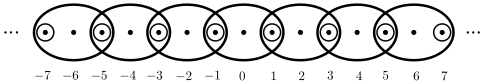
\includegraphics[width=\linewidth]{external/Digital_line.pdf}
\end{image}%
\tcblower
\end{figureptx}%
In this exercise we explore the collection \(\B = \{B(n)\}\).%
\begin{enumerate}[font=\bfseries,label=(\alph*),ref=\alph*]%
\item{}Show that the collection \(\B = \{B(n)\}\) is a basis for a topology on \(\Z\). (The resulting topology is called the \terminology{digital line topology} \(\tau_{dl}\).\footnotemark{} The digital line models a one-dimensional array of pixels, where the even integers are the pixels and the odd integers are boundaries between the pixels. Information about the \terminology{digital plane} can be found in \hyperref[chapter-chap_Product_topology]{Chapter~{\xreffont\ref{chapter-chap_Product_topology}}}.)%
\item{}Determine which of the following sets are open in the digital line topology:%
\begin{enumerate}[font=\bfseries,label=(\roman*),ref=\theenumi.\roman*]%
\item{}\(\{0\}\)%
\item{}\(\{1\}\)%
\item{}\(\{0, 2\}\)%
\item{}\(\{1, 2, 3, 4, 5\}\)%
\item{}\(\Z^+\)%
\item{}The set of odd integers.%
\end{enumerate}%
\end{enumerate}%
\end{divisionexercise}%
\footnotetext[7]{This digital line topology has applications in digital processing \textemdash{} see \pubtitle{Introduction to Topology: Pure and Applied} by Colin Adams and Robert Franzosa , Pearson Education, Inc., 2008,  Sections 1.4 and 11.3. The set \(\Z\) with the digital line topology is called the \terminology{digital line}.\label{fn-ex_digital_line_topology-b-b-a-e}}%
\begin{divisionexercise}{12}{}{}{exercise-ex_TS_Zariski}%
Let \(n\) be a positive integer and let \(\mathcal{P}_n\) be the collection of all polynomials in \(n\) real variables \(x_1\), \(x_2\), \(\ldots\), \(x_n\). As a specific example, the polynomial%
\begin{equation*}
f(x_1,x_2,x_3) = 2x_1x_3 + 5x_1x_2^2x_3^4 - x_2 + 10x_1^5x_3
\end{equation*}
is in \(\mathcal{P}_3\). If \(f(x_1, x_2, \ldots, x_n)\) is in \(\mathcal{P}_n\), let \(Z(f)\) be the set of zeros of the polynomial \(f\). That is,%
\begin{equation*}
Z(f) = \{(x_1, x_2, \ldots, x_n) \mid f(x_1,x_2, \ldots, x_n) = 0\}\text{.}
\end{equation*}
Note that \(Z(f)\) is a subset of \(\R^n\). For example, if \(n=2\) and \(f(x_1,x_2) = x_1^2 - x_2\) then \(Z(f)\) is the set of ordered pairs in \(\R^2\) satisfying \(x_1^2-x_2 = 0\), or \(x_2 = x_1^2\). This is the graph of the parabola \(y=x^2\) in the plane.%
\begin{enumerate}[font=\bfseries,label=(\alph*),ref=\alph*]%
\item{}Describe \(Z(f)\) in \(\R^2\) if \(f(x_1,x_2) = x_1^2 - 1\).%
\item{}If \(E\) is a set of polynomials in \(\mathcal{P}_n\), we let \(Z(E) = \bigcap_{f \in E} Z(f)\) be the set of common zeros of all of the polynomials in \(E\). Describe \(Z(E)\) if \(E = \{x_1+x_2+x_3, x_1-x_2-x_3, 3x_1+x_2+x_3\}\) in \(\R^3\).%
\item{}Let \(\mathcal{B}\) be the set of complements of the sets \(Z(f)\) for \(f \in \mathcal{P}_n\). Show that \(\mathcal{B}\) is a basis for a topology on \(\R^n\). The resulting topology is called the \terminology{Zariski} topology.%
\item{}Is the set \(S = \{(x_1,x_2) \in \R^2 \mid x_1 = 0 \text{ or } x_2 = 0\}\) an open set in \(\R^2\) with the Zariski topology? Explain.%
\item{}Explain why the Zariski topology when \(n=1\) is just the cofinite topology on \(\R\). That is, show that every set that is open in the cofinite topology is open in the Zariski topology and that every set that is open in the Zaariski topology is open in the cofinite topology.%
\end{enumerate}%
\end{divisionexercise}%
\begin{divisionexercise}{13}{}{}{exercise-sec_top_space_exer-m}%
For each of the following, answer true if the statement is always true. If the statement is only sometimes true or never true, answer false and provide a concrete example to illustrate that the statement is false. If a statement is true, explain why.%
\begin{enumerate}[font=\bfseries,label=(\alph*),ref=\alph*]%
\item{}The set \(\{\emptyset, \{a,b\}, \{a,b,d,f\}, \{d,f\},X\}\) is a topology on the set \(X = \{a,b,c,d,e,f\}\).%
\item{}The set \(\Z\) is an open subset of \(\R\) using the finite complement topology \(\tau_{FC}\) on \(\R\).%
\item{}The set \(\mathcal{B} = \{\{b\},\{c\}, \{a,b\}, \{b,c,d\}\}\) is a basis for the topology \(\tau\) on the set \(X = \{a,b,c,d\}\), where%
\begin{equation*}
\tau = \{\emptyset, \{b\}, \{c\}, \{a,b\}, \{b,c\}, \{a,b,c\}, \{b,c,d\}, X\}\text{.}
\end{equation*}
%
\item{}Let \(X\) be a nonempty set. If \(\tau\) is the discrete topology, then the topological set \((X,\tau)\) is metrizable.%
\item{}The point \(b\) is an interior point of the subset \(A = \{a,b,d\}\) in the topological space \((X,\tau)\), where \(X = \{a,b,c,d\}\) and%
\begin{equation*}
\tau = \{\emptyset, \{a\}, \{a,b\}, \{c\}, \{d\}, \{c,d\}, \{a,c,d\}, \{a,c\}, \{a,d\}, \{a,b,c,\}, \{a,b,d\}, X\}\text{.}
\end{equation*}
%
\item{}If \(\tau_1\) and \(\tau_2\) are topologies on a space \(X\), then \(\tau_1 \cup \tau_2\) is also a topology on \(X\).%
\item{}If \(\tau_1\) and \(\tau_2\) are topologies on a space \(X\), then \(\tau_1 \cap \tau_2\) is also a topology on \(X\).%
\end{enumerate}%
\end{divisionexercise}%
\end{exercises-section}
\end{chapterptx}
 %
%
\typeout{************************************************}
\typeout{Chapter 13 Closed Sets in Topological Spaces}
\typeout{************************************************}
%
\begin{chapterptx}{Chapter}{Closed Sets in Topological Spaces}{}{Closed Sets in Topological Spaces}{}{}{chapter-chap_Closed_sets_topology}
\renewcommand*{\chaptername}{Chapter}
\begin{objectives}{Focus Questions}{objectives-chap_Closed_sets_topology-b}
%
\begin{itemize}[label=\textbullet]
\item{}What does it mean for a set to be closed in a topological space?%
\item{}What important properties do closed sets have in relation to unions and intersections?%
\item{}What is a sequence in a topological space?%
\item{}What does it mean for a sequence to converge in a topological space?%
\item{}What is a limit of a sequence in a topological space?%
\item{}What is a limit point of a subset of a topological space? How are closed sets related to limit points?%
\item{}What is a boundary point of a subset of a topological space and what is the boundary of a subset of a topological space? How are closed sets related to boundary points?%
\item{}What does it mean for a space to be Hausdorff? What important properties do Hausdorff spaces have?%
\item{}What are the separation axioms \(T_1\), \(T_2\), \(T_3\), and \(T_4\). What is the underlying idea behind these properties?%
\end{itemize}
\end{objectives}
%
%
\typeout{************************************************}
\typeout{Section  Introduction}
\typeout{************************************************}
%
\begin{sectionptx}{Section}{Introduction}{}{Introduction}{}{}{section-sec_closed_sets_top_intro}
We defined a closed set in a metric space to be the complement of an open set. Since a topology is defined in terms of open sets, we can make the same definition of closed set in a topological space. With the definition of closed set in hand, we can then ask if it is possible to define limit points, boundary, and closure in topological spaces and determine if there are corresponding properties for these ideas in topological spaces.%
\begin{definition}{Definition}{}{definition-sec_closed_sets_top_intro-c}%
\index{closed set in a topological space}%
A subset \(C\) of a topological space \(X\) is \terminology{closed} if its complement \(X \setminus C\) is open.%
\end{definition}
\begin{exploration}{Preview Activity}{}{exploration-sec_closed_sets_top_intro-d}%
\begin{enumerate}[font=\bfseries,label=(\alph*),ref=\alph*]%
\item{}List all of the closed sets in the indicated topological space.%
\begin{enumerate}[font=\bfseries,label=(\roman*),ref=\theenumi.\roman*]%
\item{}\((X, \tau)\) with \(X= \{a,b,c,d\}\) and \(\tau = \{\emptyset, \{a\}, \{b\}, \{a,b\}, X \}\).%
\item{}\((X, \tau)\) with \(X= \{a,b,c,d,e,f\}\) and \(\tau = \{\emptyset,\{a\}, \{c,d\}, \{a,c,d\}, \{b,c,d,e,f\}, X\}\).%
\item{}\((X, \tau)\) with \(X = \R\) and \(\tau = \{\emptyset, \{0\}, \R\}\).%
\item{}\((X, \tau)\) with \(X = \{a,b,c\}\) and \(\tau = \{\emptyset, \{a\}, \{b\},\{c\}, \{a,b\}, \{a,c\}, \{b,c\}, X \}\). (What is the name of this topology?)%
\item{}\((X, \tau)\) with \(X=\Z^+\) and \(\tau = \{\emptyset, X\}\) (this topology is called the \terminology{indiscrete} or \terminology{trivial} topology).%
\end{enumerate}%
\item{}Using the examples from part (1), find (if possible), a set that is%
\begin{enumerate}[font=\bfseries,label=(\roman*),ref=\theenumi.\roman*]%
\item{}both closed and open (if possible, find one that is not the entire set or the empty set)%
\item{}closed but not open%
\item{}open but not closed%
\item{}not open and not closed%
\end{enumerate}%
\item{}In \(\R^n\) with the Euclidean metric, every single element set is closed. Does this property hold in the topological space \((X, \tau)\), where \(X = \{a, b, c\}\) and \(\tau = \{\emptyset, \{a\}, \{a, b\}, \{a, c\}, X\}\)? Explain.%
\end{enumerate}%
\end{exploration}%
\end{sectionptx}
%
%
\typeout{************************************************}
\typeout{Section  Unions and Intersections of Closed Sets}
\typeout{************************************************}
%
\begin{sectionptx}{Section}{Unions and Intersections of Closed Sets}{}{Unions and Intersections of Closed Sets}{}{}{section-sec_union_inter_closed}
\index{clopen set in a topological space}%
Now we have defined open and closed sets in topological spaces. In our preview activity we saw that a set can be both open and closed. As we did in metric spaces, we will call any set that is both open and closed a \terminology{clopen} (for closed-open) set.%
\par
By definition, any union and any finite intersection of open sets in a topological space is open, so the fact that closed sets are complements of open sets implies the following theorem.%
\begin{theorem}{Theorem}{}{}{theorem-thm_closed_TS}%
Let \(X\) be a topological space.%
\begin{enumerate}
\item{}Any intersection of closed sets in \(X\) is a closed set in \(X\).%
\item{}Any finite union of closed sets in \(X\) is a closed set in \(X\).%
\end{enumerate}
%
\end{theorem}
\begin{proof}{Proof}{}{proof-thm_closed_TS-b}
Let \(X\) be a topological space. To prove part 1, assume that \(C_{\alpha}\) is a collection of closed set in \(X\) for \(\alpha\) in some indexing set \(I\). Then%
\begin{equation*}
X \setminus \bigcap_{\alpha \in I} C_{\alpha} = \bigcup_{\alpha \in I} X \setminus C_{\alpha}\text{.}
\end{equation*}
%
\par
The latter is an arbitrary union of open sets and so it an open set. By definition, then, \(\bigcap_{\alpha \in I} C_{\alpha}\) is a closed set.%
\par
For part 2, assume that \(C_1\), \(C_2\), \(\ldots\), \(C_n\) are closed sets in \(X\) for some \(n \in \Z^+\). To show that \(C = \bigcap_{k=1}^n C_k\) is a closed set, we will show that \(X \setminus C\) is an open set. Now%
\begin{equation*}
X \setminus \bigcup_{\alpha \in I} C_{\alpha} = \bigcap_{\alpha \in I} X \setminus C_{\alpha}
\end{equation*}
is a finite intersection of open sets, and so is an open set. Therefore, \(\bigcup_{\alpha \in I} C_{\alpha}\) is a closed set.%
\end{proof}
\hyperref[theorem-thm_closed_TS]{Theorem~{\xreffont\ref{theorem-thm_closed_TS}}} tells us that any intersection of closed sets is closed, but only finite unions of closed sets are closed. How do we know that non-finite unions of closed sets aren't necessarily closed?%
\begin{activity}{Activity}{}{activity-sec_union_inter_closed-g}%
Let \(\Z\) be a topological space with the finite complement topology \(\tau_{FC}\). That is, a non-empty set \(O\) is open in \(\Z\) if \(\Z \setminus O\) is finite.%
\begin{enumerate}[font=\bfseries,label=(\alph*),ref=\alph*]%
\item{}What must be true about the cardinality of the closed sets in \((\Z, \tau_{FC})\)?%
\item{}Let \(C_n = \{2, 3, \ldots, n\}\). Is the set \(\bigcup_{n \geq 3} C_n\) a closed set in \((\Z, \tau_{FC})\)? Explain.%
\end{enumerate}%
\end{activity}%
\end{sectionptx}
%
%
\typeout{************************************************}
\typeout{Section  Limit Points and Sequences in Topological Spaces}
\typeout{************************************************}
%
\begin{sectionptx}{Section}{Limit Points and Sequences in Topological Spaces}{}{Limit Points and Sequences in Topological Spaces}{}{}{section-sec_limit_points}
Recall that we defined a limit point of a set \(A\) in a metric space \(X\) to be a point \(x \in X\) such that every neighborhood of \(x\) contains a point in \(A\) different from \(x\). Since we have defined neighborhoods in topological spaces, we can make the same definition.%
\begin{definition}{Definition}{}{definition-sec_limit_points-c}%
\index{limit point in a topological space}%
Let \(X\) be a topological space, and let \(A\) be a subset of \(X\). A \terminology{limit point} of \(A\) is a point \(x \in X\) such that every neighborhood of \(x\) contains a point in \(A\) different from \(x\).%
\end{definition}
\index{derived set} The set \(A'\) of limit points of \(A\) is called the \terminology{derived set} of \(A\).%
\begin{activity}{Activity}{}{activity-sec_limit_points-e}%
Find the limit point(s) of the following sets%
\begin{enumerate}[font=\bfseries,label=(\alph*),ref=\alph*]%
\item{}\(\{c,d\}\) in \((X, \tau)\) with \(X= \{a,b,c,d\}\) and \(\tau = \{\emptyset, \{a\}, \{b\}, \{a,b\}, X \}\)%
\item{}\(\{a,b\}\) in the set \(X= \{a,b,c,d,e,f\}\) with topology%
\begin{equation*}
\tau= \{\emptyset,\{b\}, \{a,b,c\},\{d,e,f\},\{b,d,e,f\}, X\}\text{.}
\end{equation*}
%
\item{}\(\{a,b\} \subset X\) where \(X = \{a,b,c\}\) in the discrete topology.%
\item{}\(\{-1,0,1\} \subset \Z\) with \(\tau\) the topology on \(\Z\) with basis \(\{B(n)\}\), where%
\begin{equation*}
B(n) = \begin{cases}\{n\}  \amp \text{ if \(n\) is odd } , \\ \{n-1,n,n+1\}  \amp \text{ if \(n\) is even } . \end{cases}
\end{equation*}
(This topology is called the \terminology{digital line topology} and has applications in digital processing. That the collection \(\{B(n)\}\) is a basis for a topology on \(\Z\) is the topic of \hyperlink{exercise-ex_digital_line_topology}{Exercise~{\xreffont 11}})%
\end{enumerate}%
\end{activity}%
In metric spaces, a set is closed if and only if it contains all of its limit points. So the corresponding result in topological spaces should be no surprise.%
\begin{theorem}{Theorem}{}{}{theorem-thm_TS_closed_limitpoints}%
Let \(C\) be a subset of a topological space \(X\), and let \(C'\) be the set of limit points of \(C\). Then \(C\) is closed if and only if \(C' \subseteq C\).%
\end{theorem}
\begin{proof}{Proof}{}{proof-thm_TS_closed_limitpoints-b}
Let \(X\) be a topological space, and let \(C\) be a subset of \(X\). First we assume that \(C\) is closed and show that \(C\) contains all of its limit points. Let \(x \in X\) be a limit point of \(C\). We proceed by contradiction and assume that \(x \notin C\). Then \(x \in X \setminus C\), which is an open set. This means that there is a neighborhood (namely \(X \setminus C\)) of \(x\) that contains no points in \(C\), which contradicts the fact that \(x\) is a limit point of \(C\). We conclude that \(x \in C\) and \(C\) contains all of its limit points.%
\par
For the converse, assume that \(C\) contains all of its limit points. To show that \(C\) is closed, we prove that \(X \setminus C\) is open. We again proceed by contradiction and assume that \(X \setminus C\) is not open. Then there exists \(x \in X \setminus C\) such that no neighborhood of \(x\) is entirely contained in \(X \setminus C\). This implies that every neighborhood of \(x\) contains a point in \(C\) and so \(x\) is a limit point of \(C\). It follows that \(x \in C\), contradicting the fact that \(x \in X \setminus C\). We conclude that \(X \setminus C\) is open and \(C\) is closed.%
\end{proof}
In metric spaces we saw that limit point of a set is the limit of a sequence of points in the set. To explore this idea in topological spaces, we define sequences in the same way we did in metric spaces.%
\begin{definition}{Definition}{}{definition-sec_limit_points-i}%
\index{sequence in a topological space}%
A \terminology{sequence} in a topological space \(X\) is a function \(f: \Z^+\) to \(X\).%
\end{definition}
We use the same notation and terminology related to sequences as we did in metric spaces: we will write \((x_n)\) to represent a sequence \(f\), where \(x_n = f(n)\) for each \(n \in \Z^+\). We can't define convergence in a topological space using a metric, but we can use open sets. Recall that a sequence \((x_n)\) in a metric space \((X,d)\) converges to a point \(x\) in the space if, given \(\epsilon \gt 0\) there exists a positive integer \(N\) such that \(d(x_n,x) \lt \epsilon\) for all \(n \geq N\). In other words, every open ball centered at \(x\) contains all of the entries of the sequence past a certain point. We can replace open balls with open sets and make a similar definition of convergence in topological spaces.%
\begin{definition}{Definition}{}{definition-sec_limit_points-k}%
\index{convergent sequence in a topological space}%
A sequence \((x_n)\) in a topological space \(X\) \terminology{converges} to the point \(x \in X\) if, for each open set \(O\) that contains \(x\) there exists a positive integer \(N\) such that \(x_n \in O\) for all \(n \geq N\).%
\end{definition}
\index{limit of a sequence in a topological space} If a sequence \((x_n)\) converges to a point \(x\), we call \(x\) a \terminology{limit} of the sequence \((x_n)\).%
\begin{activity}{Activity}{}{activity-act_TS_limits2}%
In metric spaces, limits of sequences are unique. We may wonder if the same result is true in topological spaces. Consider the topological space \((X,\tau)\), where \(X = \{a, b, c\}\) and \(\tau = \{\emptyset, \{c\}, \{a, c\}, \{b, c\}, X\}\). Find all limits of all constant sequences in \(X\).%
\end{activity}%
The result of \hyperref[activity-act_TS_limits2]{Activity~{\xreffont\ref{activity-act_TS_limits2}}} is that sequences do not behave in topological spaces as we would expect them to. Consequently, sequences do not play the same important role in topological spaces as they do in metric spaces. However, the concept of limit point is important, as are the notions of boundary and closure in topological spaces.%
\end{sectionptx}
%
%
\typeout{************************************************}
\typeout{Section  Closure in Topological Spaces}
\typeout{************************************************}
%
\begin{sectionptx}{Section}{Closure in Topological Spaces}{}{Closure in Topological Spaces}{}{}{section-sec_top_closure}
Once we have a definition of limit point, we can define the closure of a set just as we did in metric spaces.%
\begin{definition}{Definition}{}{definition-sec_top_closure-c}%
\index{closure in topological spaces}%
The \terminology{closure} of a subset \(A\) of a topological space \(X\) is the set%
\begin{equation*}
\overline{A} = A \cup A'\text{.}
\end{equation*}
%
\end{definition}
In other words, the closure of a set is the collection of the elements of the set and the limit points of the set. The following theorem is the analog of the theorem in metric spaces about closures.%
\begin{theorem}{Theorem}{}{}{theorem-thm_TS_closure_closed}%
Let \(X\) be a topological space and \(A\) a subset of \(X\). The closure of a \(A\) is a closed set. Moreover, the closure of \(A\) is the smallest closed subset of \(X\) that contains \(A\).%
\end{theorem}
\begin{proof}{Proof}{}{proof-thm_TS_closure_closed-b}
Let \(X\) be a topological space and \(A\) a subset of \(X\). To prove that \(\overline{A}\) is a closed set, we will prove that \(\overline{A}\) contains its limit points. Let \(x \in \overline{A}'\). To show that \(x \in \overline{A}\), we proceed by contradiction and assume that \(x \notin \overline{A}\). This implies that \(x \notin A\) and \(x \notin A'\). Since \(x \notin A'\), there exists a neighborhood \(N\) of \(x\) that contains no points of \(A\) other than \(x\). But \(A \subseteq \overline{A}\) and \(x \notin \overline{A}\), so it follows that \(N \cap A = \emptyset\). This implies that there is an open set \(O \subseteq N\) centered at \(x\) so that \(O \cap A = \emptyset\). The fact that \(x \in \overline{A}'\) means that \(O \cap \overline{A}\) contains a point \(y\) in \(\overline{A}\) different from \(x\). Since \(O \cap A = \emptyset\), we must have \(y \in A'\). But the fact that \(O\) is a neighborhood of \(y\) means that \(O\) must contain a point of \(A\) different than \(y\), which contradicts the fact that \(O \cap A = \emptyset\). We conclude that \(x \in \overline{A}\) and \(\overline{A}' \subseteq \overline{A}\). This shows that \(\overline{A}\) is a closed set.%
\par
The proof that \(\overline{A}\) is the smallest closed subset of \(X\) that contains \(A\) is left for the next activity.%
\end{proof}
\begin{activity}{Activity}{}{activity-sec_top_closure-f}%
Let \((X,d)\) be a topological space, and let \(A\) be a subset of \(X\).%
\begin{enumerate}[font=\bfseries,label=(\alph*),ref=\alph*]%
\item{}What will we have to show to prove that \(\overline{A}\) is the smallest closed subset of \(X\) that contains \(A\)?%
\item{}Suppose that \(C\) is a closed subset of \(X\) that contains \(A\). To show that \(\overline{A} \subseteq C\), why is it enough to demonstrate that \(A' \subseteq C\)?%
\item{}If \(x \in A'\), what can we say about \(x\)?%
\item{}Complete the proof that \(\overline{A} \subseteq C\).%
\end{enumerate}%
\end{activity}%
One consequence of \hyperref[theorem-thm_TS_closure_closed]{Theorem~{\xreffont\ref{theorem-thm_TS_closure_closed}}} is the following.%
\begin{corollary}{Corollary}{}{}{corollary-sec_top_closure-h}%
A subset \(C\) of a topological space \(X\) is closed if and only if \(C = \overline{C}\).%
\end{corollary}
\end{sectionptx}
%
%
\typeout{************************************************}
\typeout{Section  The Boundary of a Set}
\typeout{************************************************}
%
\begin{sectionptx}{Section}{The Boundary of a Set}{}{The Boundary of a Set}{}{}{section-sec_set_boundary}
In addition to limit points, we also defined boundary points in metric spaces. Recall that a boundary point of a set \(A\) in a metric space \(X\) could be considered to be any point in \(\overline{A} \cap \overline{X \setminus A}\). We make the same definition in a topological space.%
\begin{definition}{Definition}{}{definition-sec_set_boundary-c}%
\index{boundary point in a topological space}%
\index{boundary in a topological space}%
Let \((X, \tau)\) be a topological space, and let \(A\) be a subset of \(X\). A \terminology{boundary point} of \(A\) is a point \(x \in X\) such that every neighborhood of \(x\) contains a point in \(A\) and a point in \(X \setminus A\). The \terminology{boundary} of \(A\) is the set%
\begin{equation*}
\Bdry(A) = \{x \in X \mid x \text{ is a boundary point of }  A\}\text{.}
\end{equation*}
%
\end{definition}
As with metric spaces, the boundary points of a set \(A\) are those points that are ``between'' \(A\) and its complement.%
\begin{activity}{Activity}{}{activity-act_TS_bl_examples}%
Find the boundaries of the following sets%
\begin{enumerate}[font=\bfseries,label=(\alph*),ref=\alph*]%
\item{}\(\{c,d\}\) in \((X, \tau)\) with \(X= \{a,b,c,d\}\) and \(\tau = \{\emptyset, \{a\}, \{b\}, \{a,b\}, X \}\).%
\item{}\(\{a,b\}\) in the set \(X= \{a,b,c,d,e,f\}\) with topology%
\begin{equation*}
\tau= \{\emptyset,\{b\}, \{a,b,c\},\{d,e,f\},\{b,d,e,f\}, X\}\text{.}
\end{equation*}
%
\item{}\(\{a,b\} \subset X\) where \(X = \{a,b,c\}\) in the discrete topology.%
\item{}\(\Z\) in \(\R\) with the finite complement topology \(\tau_{FC}\).%
\end{enumerate}%
\end{activity}%
Just as with metric spaces, we can characterize the closed sets as the sets that contain their boundary.%
\begin{theorem}{Theorem}{}{}{theorem-thm_TS_Closed_boundary}%
A subset \(C\) of a topological space \(X\) is closed if and only if \(C\) contains its boundary.%
\end{theorem}
The proof of \hyperref[theorem-thm_TS_Closed_boundary]{Theorem~{\xreffont\ref{theorem-thm_TS_Closed_boundary}}} is left to \hyperlink{exercise-ex_TS_Closed_boundary}{Exercise~{\xreffont 10}}.%
\end{sectionptx}
%
%
\typeout{************************************************}
\typeout{Section  Separation Axioms}
\typeout{************************************************}
%
\begin{sectionptx}{Section}{Separation Axioms}{}{Separation Axioms}{}{}{section-sec_separation_ax}
As we have seen, sequences in topological spaces do not generally behave as we would expect them to. As a result, we look for conditions on topological spaces under which sequences do exhibit some regular behavior. In our preview activity we saw that it is possible in a topological space that single point sets do not have to be closed. In \hyperref[activity-act_TS_limits2]{Activity~{\xreffont\ref{activity-act_TS_limits2}}}, we also saw that limits of sequences in topological spaces are not necessarily unique. This type of behavior limits the results that one can prove about such spaces. As a result, we define classes of topological spaces whose behaviors are closer to what our intuition suggests.%
\begin{activity}{Activity}{}{activity-act_Hausdorff}%
\begin{enumerate}[font=\bfseries,label=(\alph*),ref=\alph*]%
\item{}Consider a metric space \((X,d)\), and let \(x\) and \(y\) be distinct points in \(X\).%
\begin{enumerate}[font=\bfseries,label=(\roman*),ref=\theenumi.\roman*]%
\item{}Explain why \(x\) and \(y\) cannot both be limits of the same sequence if we can find disjoint open balls \(B(x,r)\) centered at \(x\) and \(B(y,s)\) centered at \(y\) such that \(B_x \cap B_y = \emptyset\).%
\item{}Now show that we can find disjoint open balls \(B(x,r)\) centered at \(x\) and \(B(y,s)\) centered at \(y\) such that \(B(x,s) \cap B(y,r) = \emptyset\).%
\end{enumerate}%
\item{}Return to our example from \hyperref[activity-act_TS_limits2]{Activity~{\xreffont\ref{activity-act_TS_limits2}}} with \(X = \{a, b, c\}\) and topology%
\begin{equation*}
\tau~=~\{\emptyset, \{c\}, \{a, c\}, \{b, c\}, X\}\text{.}
\end{equation*}
We saw that every point in \(X\) is a limit of the constant sequence \((c)\). If \(x \neq c\) in \(X\), Explain why there are no disjoint open sets \(O_x\) containing \(x\) and \(O_c\) containing \(c\).%
\end{enumerate}%
\end{activity}%
It is the fact as described in \hyperref[activity-act_Hausdorff]{Activity~{\xreffont\ref{activity-act_Hausdorff}}} that we can separate disjoint points by disjoint open sets that separates metric spaces from other spaces where limits are not unique. If we restrict ourselves to spaces where we can separate points like this, then we might expect to have unique limits. Such spaces are called \terminology{Hausdorff} spaces.%
\begin{definition}{Definition}{}{definition-sec_separation_ax-e}%
\index{Hausdoff space}%
A topological space \(X\) is a \terminology{Hausdorff} space if for each pair \(x\), \(y\) of distinct points in \(X\), there exists open sets \(O_x\) of \(x\) and \(O_y\) of \(y\) such that \(O_x \cap O_y = \emptyset\).%
\end{definition}
\hyperref[activity-act_Hausdorff]{Activity~{\xreffont\ref{activity-act_Hausdorff}}} shows that every metric space is a Hausdorff space. Once we start imposing conditions on topological spaces, we restrict the number of spaces we consider.%
\begin{activity}{Activity}{}{activity-sec_separation_ax-g}%
\begin{enumerate}[font=\bfseries,label=(\alph*),ref=\alph*]%
\item{}Let \(X\) be any set and \(\tau\) the discrete topology. Is \((X, \tau)\) Hausdorff? Justify your answer.%
\item{}Let \((X, \tau)\) be a Hausdorff topological space with \(X = \{x, x_1, x_2, \ldots,
x_n\}\) a finite set. Is \(\{x\}\) an open set? Explain. What does this say about the topology \(\tau\)?%
\par\smallskip%
\noindent\textbf{\blocktitlefont Hint}.\hypertarget{hint-sec_separation_ax-g-b-b}{}\quad{}Is \(x\) a limit point of \(\{x_1, x_2, \ldots, x_n\}\)?%
\end{enumerate}%
\end{activity}%
\begin{example}{Example}{}{example-exp_K_topology}%
There are examples of Hausdorff spaces that are not the standard metric spaces. For example, Let \(K = \left\{\frac{1}{k} \mid k \text{ is a positive integer } \right\}\). We use \(K\) to make a topology on \(\R\) with basis all open intervals of the form \((a,b)\) and all sets of the form \((a,b) \setminus K\), where \(a \lt b\) are real numbers. This topology adds the extra intervals of the form \((a,b) \setminus K\) to the standard open intervals to make a new topology. This topology is known as the \(K\)-topology on \(\R\). Just as in \((\R, d_E)\), if \(x\) and \(y\) are distinct real numbers we can separate \(x\) and \(y\) with open intervals.%
\end{example}
The reason we defined Hausdorff spaces is because they have familiar properties, as the next theorems illustrate.%
\begin{theorem}{Theorem}{}{}{theorem-sec_separation_ax-j}%
Each single point subset of a Hausdorff topological space is closed.%
\end{theorem}
\begin{proof}{Proof}{}{proof-sec_separation_ax-j-b}
Let \(X\) be a Hausdorff topological space, and let \(A = \{a\}\) for some \(a \in X\). To show that \(A\) is closed, we prove that \(X \setminus A\) is open. Let \(x \in X \setminus A\). Then \(x \neq a\). So there exist open sets \(O_x\) containing \(x\) and \(O_a\) containing \(a\) such that \(O_x \cap O_a = \emptyset\). So \(a \notin O_x\) and \(O_x \subseteq X \setminus A\). Thus, every point of \(X \setminus A\) is an interior point and \(X \setminus A\) is an open set. This verifies that \(A\) is a closed set.%
\end{proof}
\begin{theorem}{Theorem}{}{}{theorem-sec_separation_ax-k}%
A sequence of points in a Hausdorff topological space can have at most one limit in the space.%
\end{theorem}
\begin{proof}{Proof}{}{proof-sec_separation_ax-k-b}
Let \(X\) be a Hausdorff topological space, and let \((x_n)\) be a sequence in \(X\). Suppose \((x_n)\) converges to \(a \in X\) and to \(b \in X\). Suppose \(a \neq b\). Then there exist open sets \(O_a\) of \(a\) and \(O_b\) of \(b\) such that \(O_a \cap O_b = \emptyset\). But the fact that \((x_n)\) converges to \(a\) implies that there is a positive integer \(N\) such that \(x_n \in O_a\) for all \(n \geq N\). But then \(x_n \notin O_b\) for any \(n \geq N\). This contradicts the fact that \((x_n)\) converges to \(b\). We conclude that \(a=b\) and that the sequence \((x_n)\) can have at most one limit in \(X\).%
\end{proof}
Hausdorff spaces are important because we can separate distinct points with disjoint open sets. It is also of interest to consider what other types of objects we can separate with disjoint open sets. For example, the indiscrete topology is quite bad in the sense that its open sets can't distinguish between distinct points. That is, if \(x\) and \(y\) are distinct points in a space with the indiscrete topology, then every open set that contains \(x\) also contains \(y\). By contrast, in a Hausdorff space we can separate distinct points with disjoint open sets. This is an example of what is called a ``separation'' property. Other types of separation properties describe different types of topological spaces. These separation properties determine what kind of objects we can separate with disjoint open sets \textemdash{} e.g., points, points and closed sets, closed sets and closed sets. The following are the most widely used separation properties. These properties rule out kinds of unwelcome properties that a topological space might have. For example, recall that limits of sequences are unique in Hausdorff spaces. (We traditionally call these separation properties ``axioms'' because we generally assume that our topological spaces have these properties. However, these are not axioms in the usual sense of the word, but rather properties.)%
\begin{definition}{Definition}{}{definition-sec_separation_ax-m}%
\index{\(T_1\)-space}%
\index{Frechet space}%
\index{\(T_2\)-space}%
\index{\(T_3\)-space}%
\index{normal topological space}%
\index{\(T_4\)-space}%
Let \(X\) be a topological space.%
\begin{enumerate}
\item{}The space \(X\) is a \terminology{\terminology{T}\(_1\)-space} or \terminology{Frechet space} if for every \(x\neq y\) in \(X\), there exist an open set \(U\) containing \(y\) such that \(x \notin U\).%
\item{}The space \(X\) is a \terminology{\terminology{T}\(_2\)-space} or a \terminology{Hausdorff space} if for every \(x\neq y\) in \(X\), there exist disjoint open sets \(U\) and \(V\) such that \(x\in U\) and \(y\in V\).%
\item{}The space \(X\) is \terminology{regular}\index{regular topological space} if for each closed set \(C\) of \(X\) and each point \(x \in X \setminus C\), there exists disjoint open sets \(U\) and \(V\) in \(X\) such that \(C \subseteq U\) and \(x \in V\). The space \(X\) is a \terminology{\terminology{T}\(_3\)-space} or a \terminology{regular Hausdorff space} if \(X\) is a regular \(T_1\) space.%
\item{}The space \(X\) is a \terminology{normal} space if for each pair \(C\) and \(D\) of disjoint closed subsets of \(X\) there exist disjoint open sets \(U\) and \(V\) such that \(C \subseteq U\) and \(D \subseteq V\). The space \(X\) is a \terminology{T\(_4\)-space} or a \terminology{normal Hausdorff space} if \(X\) is a normal \(T_1\) space.%
\end{enumerate}
%
\end{definition}
\hyperlink{exercise-ex_Metric_space_regular}{Exercise~{\xreffont 16}} shows that every metric space is both regular and normal. The use of the variable \(T\) comes from the German ``Trennungsaxiome'' for separation axioms. Note again that these are not technically axioms, but rather properties. An interesting question is why we insist that \(T_3\) and \(T_4\)-spaces also be \(T_1\). We want these axioms to provide more separation as the index increases. Consider a space \(X\) with the indiscrete topology. In this space, nothing is separated. However, this space is vacuously regular and normal. To avoid this seeming incongruity, we insist on working only with \(T_1\) spaces. Note that a space with the indiscrete topology is not \(T_1\).%
\par
It is the case that every \(T_4\)-space is \(T_3\), every \(T_3\)-space is \(T_2\), and every \(T_2\)-space is \(T_1\). Verification of these statements are left to \hyperlink{exercise-ex_T_1_2_3}{Exercise~{\xreffont 18}}. These properties are also all different. That is, there are \(T_1\)-spaces that are not \(T_2\) and \(T_2\)-spaces that are not \(T_3\). These problems are given in \hyperlink{exercise-ex_not_T_1_2_3}{Exercise~{\xreffont 19}}. The fact that there are \(T_3\)-spaces that are not \(T_4\) is a bit difficult. An example is the \terminology{Niemytzki plane}. The Niemytzki plane is the upper half plane \(X = \{(x,y) \in \R^2 \mid y \geq 0\}\). Let \(L\) be the boundary of \(X\). That is, \(L = \{(x,y) \in \R^2 \mid y = 0\}\). A basis for the topology on \(X\) consists of the standard open disks centered at points with \(y \gt 0\) along with the open disks in \(X \setminus L\) that are tangent to \(L\) together with their points of tangency. We won't verify that the Niemytzki plane is \(T_3\) but not \(T_4\). The interested reader can find an accessible proof in the article ``Another Proof that the Niemytzki Plane is not Normal'' by David H. Vetterlein in the \pubtitle{Pi Mu Epsilon Journal}, Vol. 10, No. 2 (SPRING 1995), pp. 119-121.%
\end{sectionptx}
%
%
\typeout{************************************************}
\typeout{Section  Summary}
\typeout{************************************************}
%
\begin{sectionptx}{Section}{Summary}{}{Summary}{}{}{section-sec_closed_sets_top_summ}
Important ideas that we discussed in this section include the following.%
\begin{itemize}[label=\textbullet]
\item{}A subset \(C\) of a topological space \(X\) is closed if \(X \setminus C\) is open.%
\item{}Any intersection of closed sets is closed, while unions of finitely many closed sets are closed.%
\item{}A sequence in a topological space \(X\) is a function \(f: \Z^+\) to \(X\).%
\item{}A sequence \((x_n)\) in a topological space \(X\) converges to a point \(x\) in \(X\) if for each open set \(O\) containing \(x\), there exists a positive integer \(N\) such that \(x_n \in O\) for all \(n \geq N\).%
\item{}If a sequence \((x_n)\) in a topological space \(X\) converges to a point \(x\), then \(x\) is a limit of the sequence \((x_n)\).%
\item{}A limit point of a subset \(A\) of a topological space \(X\) is a point \(x \in X\) such that every neighborhood of \(x\) contains a point in \(A\) different from \(x\). A subset \(C\) of a topological space \(X\) is closed if and only if \(C\) contains all of its limit points.%
\item{}A boundary point of a subset \(A\) of a topological space \(X\) is a point \(x \in X\) such that every neighborhood of \(x\) contains a point in \(A\) and a point in \(X \setminus A\). The boundary of \(A\) is the set%
\begin{equation*}
\Bdry(A) = \{x \in X \mid x \text{ is a boundary point of }  A\}\text{.}
\end{equation*}
A subset \(C\) of \(X\) is closed if and only if \(C\) contains its boundary.%
\item{}A topological space \(X\) is Hausdorff if we can separate distinct points with open sets in the space. That is, if for each pair \(x\), \(y\) of distinct points in \(X\), there exists open sets \(O_x\) of \(x\) and \(O_y\) of \(y\) such that \(O_x \cap O_y = \emptyset\). Hausdorff spaces are important because sequences have unique limits in Hausdorff spaces and single point sets are closed.%
\item{}Separation axioms tell us what kinds of objects can be separated by open sets.%
\begin{itemize}[label=$\circ$]
\item{}In a \(T_1\)-space, we can separate two distinct points with one open set. That is, given distinct points \(x\) and \(y\) in a \(T_1\) topological space \(X\), there is an open set \(U\) that separates \(y\) from \(x\) in the sense that \(y \in U\) but \(x \notin U\).%
\item{}In a \(T_2\)-space \(X\) we can separate points more distinctly. That is, if \(x\) and \(y\) are different points in \(X\), there exist disjoint open sets \(U\) and \(V\) such that \(x \in U\) and \(y \in V\).%
\item{}In a \(T_3\)-space \(X\) we can separate a point from a closed set that does not contain that point. That is, if \(C\) is a closed subset of \(X\) and \(x\) is a point not in \(C\), there exists disjoint open sets \(U\) and \(V\) in \(X\) such that \(C \subseteq U\) and \(x \in V\).%
\item{}In a \(T_4\)-space \(X\) we can separate disjoint closed sets. That is, if \(C\) and \(D\) are disjoint closed subsets of \(X\), there exist disjoint open sets \(U\) and \(V\) such that \(C \subseteq U\) and \(D \subseteq V\).%
\end{itemize}
%
\end{itemize}
%
\end{sectionptx}
%
%
\typeout{************************************************}
\typeout{Exercises  Exercises}
\typeout{************************************************}
%
\begin{exercises-section}{Exercises}{Exercises}{}{Exercises}{}{}{exercises-sec_closed_sets_top_exer}
\begin{divisionexercise}{1}{}{}{exercise-sec_closed_sets_top_exer-a}%
Determine exactly which finite topological spaces are Hausdorff. Prove your result.%
\end{divisionexercise}%
\begin{divisionexercise}{2}{}{}{exercise-sec_closed_sets_top_exer-b}%
Let \((X, \tau)\) be a topological space and let \(A\) be a subset of \(X\). Prove that \(\overline{A} = A \cup \Bdry(A)\).%
\end{divisionexercise}%
\begin{divisionexercise}{3}{}{}{exercise-sec_closed_sets_top_exer-c}%
Let \(A\) a subset of a topological space. Prove that \(\Bdry(A) = \emptyset\) if and only if \(A\) is open and closed.%
\end{divisionexercise}%
\begin{divisionexercise}{4}{}{}{exercise-sec_closed_sets_top_exer-d}%
Let \(X\) be a nonempty set with at least two elements and let \(p\) be a fixed element in \(X\). Let \(\tau_p\) be the particular point topology and \(\tau_{\overline{p}}\) the excluded point topology on \(X\). That is%
\begin{itemize}[label=\textbullet]
\item{}\(\tau_{p}\) is the collection of subsets of \(X\) consisting of \(\emptyset\), \(X\), and all of the subsets of \(X\) that contain \(p\).%
\item{}\(\tau_{\overline{p}}\) is the collection of subsets of \(X\) consisting of \(\emptyset\), \(X\), and all of the subsets of \(X\) that do not contain \(p\).%
\end{itemize}
That the particular point and excluded point topologies are topologies is the subject of \hyperlink{exercise-ex_particular_point_topology}{Exercise~{\xreffont 9}} and \hyperlink{exercise-ex_excluded_point_topology}{Exercise~{\xreffont 10}}. Let \(A = (0,1]\) be a subset of \(\R\). Find, with proof, \(\overline{A}\), \(\Int(A)\), and \(\Bdry(A)\) when%
\begin{enumerate}[font=\bfseries,label=(\alph*),ref=\alph*]%
\item{}\(\R\) has the topology \(\tau_{p}\) with \(p = 0\)%
\item{}\(\R\) has the topology \(\tau_{\overline{p}}\) with \(p = 0\).%
\end{enumerate}%
\end{divisionexercise}%
\begin{divisionexercise}{5}{}{}{exercise-ex_Closed_Sets_Sorgenfrey}%
\index{topology!lower limit}%
\index{Sorgenfrey line}%
Let \(\B = \{[a,b) \mid a \lt b \text{ in } \R\}\).%
\begin{enumerate}[font=\bfseries,label=(\alph*),ref=\alph*]%
\item{}Show that \(\B\) is a basis for a topology \(\tau_{\ell \ell}\) on \(\R\). This topology is called the \terminology{lower limit} topology on \(\R\). The line \(\R\) with the topology \(\tau_{\ell \ell}\) is sometimes called the \terminology{Sorgenfrey line} (after the mathematician Robert Sorgenfrey).%
\item{}Show that every open interval \((a,b)\) is also an open set in the lower limit topology.%
\item{}If \(\tau_1\) and \(\tau_2\) are topologies on a set \(X\) such that \(\tau_1 \subseteq \tau_2\), then \(\tau_1\) is said to be a \terminology{coarser} topology that \(\tau_2\), or \(\tau_2\) is a \terminology{finer} topology that \(\tau_1\). Part (b) shows that the lower limit topology may be a finer topology than the Euclidean metric topology. Determine if this is true, that the lower limit topology is actually a finer topology than the Euclidean metric topology on \(\R\). Justify your answer.%
\item{}Let \(a \lt b\) be in \(\R\). Is the set \([a,b)\) clopen in \((\R, \tau_{\ell \ell})\)? Prove your answer.%
\end{enumerate}%
\end{divisionexercise}%
\begin{divisionexercise}{6}{}{}{exercise-sec_closed_sets_top_exer-f}%
A subset \(A\) of a topological space \(X\) is said to be \terminology{dense} in \(X\) if \(\overline{A} = X\).%
\begin{enumerate}[font=\bfseries,label=(\alph*),ref=\alph*]%
\item{}Show that \(\Q\) is dense in \(\R\) using the Euclidean metric topology.%
\item{}Is \(\Z\) dense in \(\R\) using the Euclidean metric topology? Prove your answer.%
\item{}Let \(A\) be a subset of a topological space \(A\). Prove that \(A\) is dense in \(X\) if and only if \(A \cap O \neq \emptyset\) for every open set \(O\).%
\end{enumerate}%
\end{divisionexercise}%
\begin{divisionexercise}{7}{}{}{exercise-sec_closed_sets_top_exer-g}%
Let \(X\) be a topological space and let \(A\) be a subset of \(X\).%
\begin{enumerate}[font=\bfseries,label=(\alph*),ref=\alph*]%
\item{}Show that the sets \(\Int(A)\), \(\Bdry(A)\), and \(\Int(A^c)\) are mutually disjoint (that is, the intersection of any two of these sets is empty).%
\item{}Prove that \(X = \Int(A) \cup \Bdry(A) \cup \Int(A^c)\).%
\end{enumerate}%
\end{divisionexercise}%
\begin{divisionexercise}{8}{}{}{exercise-ex_Closed_sets_Hausdorff_subspace}%
Prove that a subspace of a Hausdorff space is a Hausdorff space.%
\end{divisionexercise}%
\begin{divisionexercise}{9}{}{}{exercise-sec_closed_sets_top_exer-i}%
Let \(X\) be a nonempty set with at least two elements and let \(p\) be a fixed element in \(X\). Let \(\tau_p\) be the particular point topology and \(\tau_{\overline{p}}\) the excluded point topology on \(X\). That is%
\begin{itemize}[label=\textbullet]
\item{}\(\tau_{p}\) is the collection of subsets of \(X\) consisting of \(\emptyset\), \(X\), and all of the subsets of \(X\) that contain \(p\).%
\item{}\(\tau_{\overline{p}}\) is the collection of subsets of \(X\) consisting of \(\emptyset\), \(X\), and all of the subsets of \(X\) that do not contain \(p\).%
\end{itemize}
That the particular point and excluded point topologies are topologies is the subject of \hyperlink{exercise-ex_particular_point_topology}{Exercise~{\xreffont 9}} and \hyperlink{exercise-ex_excluded_point_topology}{Exercise~{\xreffont 10}}. Determine, with proof, if \(X\) is a Hausdorff space when%
\begin{enumerate}[font=\bfseries,label=(\alph*),ref=\alph*]%
\item{}\(X\) has the topology \(\tau_{p}\)%
\item{}\(X\) has the topology \(\tau_{\overline{p}}\).%
\end{enumerate}%
\end{divisionexercise}%
\begin{divisionexercise}{10}{}{}{exercise-ex_TS_Closed_boundary}%
Prove that a subset \(C\) of a topological space \(X\) is closed if and only if \(C\) contains its boundary.%
\end{divisionexercise}%
\begin{divisionexercise}{11}{}{}{exercise-sec_closed_sets_top_exer-k}%
Recall that a point \(a\) in a subset \(A\) of a metric space \(X\) is an isolated point of \(A\) if there is a neighborhood \(N\) of \(a\) in \(X\) such that \(N \cap A = \{a\}\). We can make the same definition in any topological space.%
\begin{definition}{Definition}{}{definition-sec_closed_sets_top_exer-k-a-b}%
A point \(a\) in a subset \(A\) of a topological space \(X\) is an isolated point of \(A\) \index{isolated point} if there is a neighborhood \(N\) of \(a\) such that \(N \cap A = \{a\}\).%
\end{definition}
\begin{enumerate}[font=\bfseries,label=(\alph*),ref=\alph*]%
\item{}If \(A\) is a subset of a topological space \(X\), prove that a point \(a \in A\) is an isolated point of \(A\) if and only if \(\{a\}\) is an open set in \(A\).%
\item{}We proved that in a metric space every boundary point of a set \(A\) is either a limit point or an isolated point of \(A\). (See \hyperlink{exercise-ex_MS_boundary_limit_isolated}{Exercise~{\xreffont 12}}.) Is the same statement true in a topological space? Prove your answer.%
\end{enumerate}%
\end{divisionexercise}%
\begin{divisionexercise}{12}{}{}{exercise-sec_closed_sets_top_exer-l}%
For each integer \(a\), let \(a\Z = \{ka \mid k \in \Z\}\). That is, \(a\Z\) is the set of all integer multiples of \(a\). That \(\{a\Z \mid a \in \Z\}\) is a basis for a topology \(\tau\) on \(\Z\) is the topic of Exercise (ex\textunderscore{}aZ\textunderscore{}top). In this exercise work in the topological space \((\Z, \tau)\)%
\begin{enumerate}[font=\bfseries,label=(\alph*),ref=\alph*]%
\item{}Let \(A = \mathbb{E}\), the set of even integers.%
\begin{enumerate}[font=\bfseries,label=(\roman*),ref=\theenumi.\roman*]%
\item{}Find, with justification, \(\Int(A)\).%
\item{}Find, with justification, \(\overline{A}\).%
\end{enumerate}%
\item{}Let \(B = \mathbb{N} = \{n \in \Z \mid n \geq 1\}\). That is, \(\mathbb{N}\) is the set of natural numbers.%
\begin{enumerate}[font=\bfseries,label=(\roman*),ref=\theenumi.\roman*]%
\item{}Find, with justification, \(\Int(B)\).%
\item{}Find, with justification, \(\overline{B}\).%
\end{enumerate}%
\end{enumerate}%
\end{divisionexercise}%
\begin{divisionexercise}{13}{}{}{exercise-sec_closed_sets_top_exer-m}%
Consider the Double Origin topology\index{topology!Double Origin} defined as follows. Let \(X = \R^2 \cup \{0^*\}\), where \(0^*\) is considered as a point that is not in \(\R^2\) (\(0^*\) is our double origin). As a basis for the open sets, we use the standard open balls for every point except \(0\) and \(0^*\). For the point \(0\), we define open sets to be%
\begin{equation*}
N(0,r) = \left\{(x,y) \in \R^2 \mid x^2+y^2 \lt  \frac{1}{r^2}, y \gt 0\right\}  \cup \{0\}
\end{equation*}
and for \(0^*\) we define open sets to be%
\begin{equation*}
N(0^*, r) =  \left\{(x,y) \in \R^2 \mid x^2+y^2 \lt  \frac{1}{r^2}, y \lt  0\right\}  \cup \{0^*\}\text{.}
\end{equation*}
So \(N(0,r)\) is the top half of a disk of radius \(\frac{1}{r}\) centered at the origin, excluding the \(y\)-axis but including the origin, and \(N(0^*,r)\) is the bottom half of a disk of radius \(\frac{1}{r}\) centered at the origin, excluding the \(y\)-axis and including the point \(0^*\).%
\begin{enumerate}[font=\bfseries,label=(\alph*),ref=\alph*]%
\item{}Show that the collection of sets described as a basis for the Double Origin topology is actually a basis for a topology.%
\item{}Is \(X\) with the Double Origin topology Hausdorff? Prove your answer.%
\end{enumerate}%
\end{divisionexercise}%
\begin{divisionexercise}{14}{}{}{exercise-sec_closed_sets_top_exer-n}%
\begin{enumerate}[font=\bfseries,label=(\alph*),ref=\alph*]%
\item{}Show that finite sets are closed in \(\R^n\) with the Zariski topology.%
\item{}Show that \(\R^n\) with the Zariski topology is not Hausdorff. (\hyperlink{exercise-ex_TS_Zariski}{Exercise~{\xreffont 12}} shows that a basis for the Zariski topology on \(\R^n\) is the collection of sets of the form \(\R^n \setminus Z(f)\), where \(Z(f)\) is the set of zeros of the polynomial \(f\) in \(n\) variables.)%
\end{enumerate}%
\end{divisionexercise}%
\begin{divisionexercise}{15}{}{}{exercise-sec_closed_sets_top_exer-o}%
Consider the digital line topology \(\tau_{dl}\) on \(\Z\) with basis \(\{B(n)\}\), where%
\begin{equation*}
B(n) = \begin{cases}\{n\}  \amp \text{ if \(n\) is an odd integer } , \\ \{n-1,n,n+1\}  \amp \text{ if \(n\) is an even integer } . \end{cases}
\end{equation*}
%
\begin{enumerate}[font=\bfseries,label=(\alph*),ref=\alph*]%
\item{}Let \(A = \{-1,0,1\}\) of \((\Z, \tau_{dl})\).%
\begin{enumerate}[font=\bfseries,label=(\roman*),ref=\theenumi.\roman*]%
\item{}Find the limit points and boundary points of \(A\). Prove your conjectures. Is every limit point of \(A\) a boundary point of \(A\)? Is every boundary point of \(A\) a limit point of \(A\)?%
\item{}Find \(\overline{A}\) and write \(X \setminus \overline{A}\) as a union of open sets.%
\end{enumerate}%
\item{}Now consider the subset \(B = \{0\}\) of \((\Z, \tau_{dl})\).%
\begin{enumerate}[font=\bfseries,label=(\roman*),ref=\theenumi.\roman*]%
\item{}Find the limit points and boundary points of \(B\). Prove your conjectures. Is every limit point of \(B\) a boundary point of \(B\)? Is every boundary point of \(B\) a limit point of \(B\)?%
\item{}Find \(\overline{B}\) and write \(X \setminus \overline{B}\) as a union of open sets.%
\end{enumerate}%
\end{enumerate}%
\end{divisionexercise}%
\begin{divisionexercise}{16}{}{}{exercise-ex_Metric_space_regular}%
Let \((X,d)\) be a metric space. Recall from \hyperlink{exercise-ex_distance_pt_to_set}{Exercise~{\xreffont 8}} in \hyperref[chapter-chap_closed_sets]{Chapter~{\xreffont\ref{chapter-chap_closed_sets}}}, that if \(C\) is a closed subset of a metric space \(X\) and \(x\) is an element of \(X \setminus C\), then \(d(x,C) = 0\) if and only if \(x \in C\). Use this idea to do the following.%
\begin{enumerate}[font=\bfseries,label=(\alph*),ref=\alph*]%
\item{}Prove that every metric space is regular.%
\item{}Prove that every metric space is a normal space.%
\end{enumerate}%
\end{divisionexercise}%
\begin{divisionexercise}{17}{}{}{exercise-sec_closed_sets_top_exer-q}%
Let  \(K = \left\{\frac{1}{k} \mid k \text{ is a positive integer} \right\}\). Let \(\B\) be the collection of all open intervals of the form \((a,b)\) and all sets of the form \((a,b) \setminus K\), where \(a \lt b\) are real numbers as in \hyperref[example-exp_K_topology]{Example~{\xreffont\ref{example-exp_K_topology}}}.  That \(\B\) generates a topology \(\tau_K\) on \(\R\) follows from the fact that \(\tau_K\) is finer than the Euclidean topology.%
\begin{enumerate}[font=\bfseries,label=(\alph*),ref=\alph*]%
\item{}Show that \((\R, \tau_K)\) is a Hausdorff space.%
\item{}\hyperlink{exercise-ex_Metric_space_regular}{Exercise~{\xreffont 16}} shows that every metric space is regular. In this part of the exercise, show that \((R, \tau_K)\) is not a regular space. We can conclude that \((\R, \tau_K)\) is not metrizable.%
\par\smallskip%
\noindent\textbf{\blocktitlefont Hint}.\hypertarget{hint-sec_closed_sets_top_exer-q-c-b}{}\quad{}Consider \(0\) and \(K\).%
\end{enumerate}%
\end{divisionexercise}%
\begin{divisionexercise}{18}{}{}{exercise-ex_T_1_2_3}%
\begin{enumerate}[font=\bfseries,label=(\alph*),ref=\alph*]%
\item{}Prove that a topological space \(X\) is \(T_1\) if and only if each singleton set is closed.%
\item{}Show that every \(T_2\)-space is \(T_1\), that every \(T_3\)-space is \(T_2\), and that every \(T_4\)-space is \(T_3\).%
\end{enumerate}%
\end{divisionexercise}%
\begin{divisionexercise}{19}{}{}{exercise-ex_not_T_1_2_3}%
In this exercise we illustrate spaces that are \(T_1\) but not \(T_2\) and \(T_2\) but not \(T_3\).%
\begin{enumerate}[font=\bfseries,label=(\alph*),ref=\alph*]%
\item{}Show that \(\R\) with the finite complement topology is \(T_1\) but not \(T_2\).%
\item{}Define the space \(\R_K\) as in \hyperref[example-exp_K_topology]{Example~{\xreffont\ref{example-exp_K_topology}}} to be the set of reals with topology \(\tau\) with a basis that consists of the standard open intervals in \(\R\) along with all sets of the form \((a,b) \setminus K\), where \((a,b)\) is any open interval and \(K = \left\{\frac{1}{k} \mid k \in \Z^+\right\}\). Show that \(\R_K\) is \(T_2\) but not \(T_3\).%
\end{enumerate}%
\end{divisionexercise}%
\begin{divisionexercise}{20}{}{}{exercise-sec_closed_sets_top_exer-t}%
For each of the following, answer true if the statement is always true. If the statement is only sometimes true or never true, answer false and provide a concrete example to illustrate that the statement is false. If a statement is true, explain why.%
\begin{enumerate}[font=\bfseries,label=(\alph*),ref=\alph*]%
\item{}Every limit point of a subset \(A\) of a topological space \(X\) is also a boundary point of \(A\).%
\item{}Every boundary point of a subset \(A\) of a topological space \(X\) is also a limit point of \(A\).%
\item{}If \(X\) is a topological space and \(A \subseteq X\) such that \(\Int(A)=\overline{A}\), then \(A\) is both open and closed.%
\item{}If \(X\) is a topological space and \(A\) and \(B\) are subsets of \(X\) with \(\overline{A}=\overline{B}\) and \(\Int(A) = \Int(B)\), then \(A = B\).%
\item{}If \(A\) and \(B\) are subsets of a topological space \(X\), then \(\overline{A \cap B} = \overline{A} \cap \overline{B}\).%
\item{}If \(A\) and \(B\) are subsets of a topological space \(X\), then \(\overline{A \cup B} = \overline{A} \cup \overline{B}\).%
\end{enumerate}%
\end{divisionexercise}%
\end{exercises-section}
\end{chapterptx}
 %
%
\typeout{************************************************}
\typeout{Chapter 14 Continuity and Homeomorphisms}
\typeout{************************************************}
%
\begin{chapterptx}{Chapter}{Continuity and Homeomorphisms}{}{Continuity and Homeomorphisms}{}{}{chapter-chap_continuity_topology}
\renewcommand*{\chaptername}{Chapter}
\begin{objectives}{Focus Questions}{objectives-chap_continuity_topology-b}
%
\begin{itemize}[label=\textbullet]
\item{}How do we define a continuous function between topological spaces?%
\item{}What is the difference between metric equivalence and topological equivalence?%
\item{}What is a homeomorphism? What does it mean for two topological spaces to be homeomorphic?%
\item{}What is a topological invariant? Why are topological invariants useful?%
\end{itemize}
\end{objectives}
%
%
\typeout{************************************************}
\typeout{Section  Introduction}
\typeout{************************************************}
%
\begin{sectionptx}{Section}{Introduction}{}{Introduction}{}{}{section-sec_cont_top_intro}
Recall that we could characterize a function \(f\) from a metric space \((X,d_X)\) to a metric space \((Y,d_Y)\) as continuous at \(a \in X\) if \(f^{-1}(N)\) is a neighborhood of \(a\) in \(X\) whenever \(N\) is a neighborhood of \(f(a)\) in \(Y\). We have defined neighborhoods in topological spaces, so we can use this characterization as our definition of a continuous function from one topological space to another.%
\begin{definition}{Definition}{}{definition-def_Continuity_topology}%
\index{continuity in a topological space}%
A function \(f\) from a topological space \((X, \tau_X)\) to a topological space \((Y, \tau_Y)\) is \terminology{continuous at a point} \(a \in X\) if \(f^{-1}(N)\) is a neighborhood of \(a\) in \(X\) whenever \(N\) is a neighborhood of \(f(a)\) in \(Y\). The function \(f\) is continuous if \(f\) is \terminology{continuous} at each point in \(X\).%
\end{definition}
We saw that in metric spaces, a useful characterization of continuity was in terms of open sets. It is not surprising that we have the same characterization in topological spaces. You may assume the result of \hyperref[theorem-thm_PA_TS_Open_continuity]{Theorem~{\xreffont\ref{theorem-thm_PA_TS_Open_continuity}}} (the topological space version of \hyperref[theorem-thm_Open_continuity]{Theorem~{\xreffont\ref{theorem-thm_Open_continuity}}} for metric spaces) for this activity.%
\begin{theorem}{Theorem}{}{}{theorem-thm_PA_TS_Open_continuity}%
Let \(f\) be a function from a topological space \((X,\tau_X)\) to a topological space \((Y,\tau_Y)\). Then \(f\) is continuous if and only if \(f^{-1}(O)\) is an open set in \(X\) whenever \(O\) is an open set in \(Y\).%
\end{theorem}
\begin{exploration}{Preview Activity}{}{exploration-sec_cont_top_intro-f}%
\begin{enumerate}[font=\bfseries,label=(\alph*),ref=\alph*]%
\item{}Let%
\begin{equation*}
(X, \tau_X) = (\{1,2,3,4\}, \{\emptyset, \{1\}, \{2\}, \{1,2\}, X \})
\end{equation*}
and let%
\begin{equation*}
(Y, \tau_Y) = (\{2,4,6,8\}, \{\emptyset, \{4\}, \{6\}, \{4,6\}, Y\})\text{.}
\end{equation*}
Define \(f: X \to Y\) by \(f(x) = 2x\).%
\begin{enumerate}[font=\bfseries,label=(\roman*),ref=\theenumi.\roman*]%
\item{}Is \(f\) continuous at \(4\)?%
\item{}Is \(f\) a continuous function?%
\end{enumerate}%
\item{}Let%
\begin{equation*}
(X, \tau_X) = (\{1,2,3,4\}, \{\emptyset, \{1\}, \{2\}, \{1,2\}, \{3,4\}, X \})
\end{equation*}
and let%
\begin{equation*}
(Y, \tau_Y) = (\{a,b,c\}, \{\emptyset, \{a\}, \{a,c\}, Y\})\text{.}
\end{equation*}
Define \(f: X \to Y\) by \(f(1) = a\), \(f(2) = c\), \(f(3) = f(4) = b\).%
\begin{enumerate}[font=\bfseries,label=(\roman*),ref=\theenumi.\roman*]%
\item{}Show that \(f\) is a continuous function.%
\item{}Even though \(f\) is continuous, it is possible that \(f(O)\) may not be open for every open set in \(X\). Find such an example for this function \(f\).%
\end{enumerate}%
\item{}Functions \(f\) that have the property that \(f(O)\) is open whenever \(O\) is open in \(X\) are called \terminology{open} functions.%
\begin{definition}{Definition}{}{definition-sec_cont_top_intro-f-c-a-b}%
\index{function!open}%
\index{open function}%
Let \(f: X \to Y\) be a function from a topological space \(X\) to a topological space \(Y\). Then \(f\) is an \terminology{open} function if \(f(U)\) is open in \(Y\) whenever \(U\) is open in \(X\).%
\end{definition}
There is a similar definition of a \terminology{closed} function.%
\item{}Let \(X= \{1,2,3,4,5\}\) and \(\tau = \{\emptyset,\{1\}, \{3,5\}, \{1,3,5\}, X\}\). Define \(f: X \to X\) by \(f(x) = \la x-3 \ra+1\). At which points is \(f\) continuous? Is \(f\) a continuous function?%
\item{}Let \(f:(\Z,\tau_{FC}) \to (\Z, d_E)\) where \(f(n) = n\) and \(\tau_{FC}\) is the finite complement topology. Is \(f\) a continuous function? If \(f\) is not continuous, exhibit a specific point at which \(f\) fails to be continuous. Explain.%
\item{}Let \(f:(\Z, d_E) \to (\Z,\tau_{FC})\) where \(f(n) = n\) and \(\tau_{FC}\) is the finite complement topology. Is \(f\) a continuous function? If \(f\) is not continuous, exhibit a specific point at which \(f\) fails to be continuous. Explain.%
\item{}It can sometimes be easier to show that a function \(f\) mapping a topological space \((X,d_X)\) to a topological space \((Y,d_Y)\) is continuous by working with a basis instead of all open sets. Let \(\B\) be a basis for the topology on \(Y\). Is it the case that if \(f^{-1}(B)\) is open for every \(B \in \B\), then \(f\) is continuous? Verify your result.%
\end{enumerate}%
\end{exploration}%
To complete the introduction to this section, we prove \hyperref[theorem-thm_PA_TS_Open_continuity]{Theorem~{\xreffont\ref{theorem-thm_PA_TS_Open_continuity}}}. We prove one direction now and leave the other for the next activity.%
\par
Let \(f\) be a function from a topological space \((X, \tau_X)\) to a topological space \((Y, \tau_Y)\). We first assume that \(f\) is continuous and show that \(f^{-1}(O)\) is an open set in \(X\) whenever \(O\) is an open set in \(Y\). Suppose that \(O\) is an open set in \(Y\). To show that \(f^{-1}O)\) is open in \(X\), we will show that \(f^{-1}(O)\) is a neighborhood of each of its points. Let \(a \in f^{-1}(O)\). Then \(f(a) \in O\). Since \(O\) is an open set, \(O\) is a neighborhood of \(f(a)\). The fact that \(f\) is continuous means that \(f^{-1}(O)\) is a neighborhood of \(a\). So \(f^{-1}(O)\) is a neighborhood of each of its points and \(f^{-1}(O)\) is an open set.%
\begin{activity}{Activity}{}{activity-sec_cont_top_intro-i}%
Now we prove the remaining implication in \hyperref[theorem-thm_PA_TS_Open_continuity]{Theorem~{\xreffont\ref{theorem-thm_PA_TS_Open_continuity}}}. That is, let \(f\) be a function from a topological space \((X, \tau_X)\) to a topological space \((Y, \tau_Y)\), and assume that \(f^{-1}(O)\) is open whenever \(O\) is open in \(Y\). We will prove that \(f\) is a continuous function.%
\begin{enumerate}[font=\bfseries,label=(\alph*),ref=\alph*]%
\item{}Using the definition, what does it take to show that \(f\) is a continuous function?%
\item{}Let \(a \in X\) and suppose that \(N\) is a neighborhood of \(f(a)\) in \(Y\). What can we conclude from \(N\) being a neighborhood?%
\item{}Use the assumption about \(f\) in this activity to explain why \(f^{-1}(N)\) is a neighborhood of \(a\) in \(X\).%
\item{}Explain how we have shown that \(f\) is a continuous function.%
\end{enumerate}%
\end{activity}%
The following theorem is the topological analog of \hyperref[theorem-thm_closed_sets_continuity_MS]{Theorem~{\xreffont\ref{theorem-thm_closed_sets_continuity_MS}}}. The proof is left for \hyperlink{exercise-ex_closed_sets_continuity_TS}{Exercise~{\xreffont 4}}.%
\begin{theorem}{Theorem}{}{}{theorem-thm_closed_sets_continuity_TS}%
Let \(f\) be a function from a topological space \((X,\tau_X)\) to a topologicval space \((Y,\tau_Y)\). Then \(f\) is continuous if and only if \(f^{-1}(C)\) is closed in \(X\) whenever \(C\) is a closed set in \(Y\).%
\end{theorem}
\end{sectionptx}
%
%
\typeout{************************************************}
\typeout{Section  Metric Equivalence}
\typeout{************************************************}
%
\begin{sectionptx}{Section}{Metric Equivalence}{}{Metric Equivalence}{}{}{section-sec_metric_equiv}
We have seen that we can make a set into a metric space with different metrics. For example, the spaces \((\R^2, d_E)\), \((\R^2, d_T)\), \((\R^2, d_M)\), and \((\R^2, d)\) are all metric spaces, where \(d_E\) is the Euclidean metric, \(d_T\) the taxicab metric, \(d_M\) the max metric, and \(d\) the discrete metric. But are these metric spaces really ``different'' metric spaces? What do we mean by ``different''?%
\begin{activity}{Activity}{}{activity-sec_metric_equiv-c}%
We might consider two metric spaces \((X, d_X)\) and \((Y, d_Y)\) to be equivalent if we can find a bijection between the two sets \(X\) and \(Y\) that preserves the metric properties. That is, find a bijective function \(f : X \to Y\) such that \(d_X(a,b) = d_Y(f(a),
f(b))\) for all \(a,b \in X\). In other words, \(f\) preserves distances.%
\begin{enumerate}[font=\bfseries,label=(\alph*),ref=\alph*]%
\item{}Let \(X = ((0,1), d_X)\) and \(Y = ((0,2), d_Y)\), with both \(d_X\) and \(d_Y\) the Euclidean metric. Is it possible to find a bijection \(f : X \to Y\) that preserves the metric properties? Explain.%
\item{}Now let \(X = ((0,1), d_X)\) and \(Y = ((0,2), d_Y)\), where \(d_X\) is defined by \(d_X(a,b) = 2 | a-b |\) and \(d_Y = d_E\). You may assume that \(d_X\) is a metric. Is it possible to find a bijection \(f : X \to Y\) that preserves the metric properties? Explain.%
\end{enumerate}%
\end{activity}%
If there is a bijection between metric spaces that preserves distances, we say that the metric spaces are \terminology{metrically equivalent}.%
\begin{definition}{Definition}{}{definition-def_MS_metric_equivalence}%
\index{metrically equivalent}%
Two metric spaces \((X,d_X)\) and \((Y,d_Y)\) are \terminology{metrically equivalent} if there is a bijection \(f : X \to Y\) such that%
\begin{equation*}
d_X(x,y) = d_Y(f(x),f(y))
\end{equation*}
for all \(x,y \in X\).%
\end{definition}
Because \(f\) is a bijection, it will also be the case in \hyperref[definition-def_MS_metric_equivalence]{Definition~{\xreffont\ref{definition-def_MS_metric_equivalence}}} that%
\begin{equation*}
d_Y(u,v) = d_X(f^{-1}(u), f^{-1}(v))
\end{equation*}
for all \(u\) and \(v\) in \(Y\). The proof is left for \hyperlink{exercise-ex_isometry_reverse}{Exercise~{\xreffont 1}}.%
\par
Any function \(f\) that preserves distances (like the one in \hyperref[definition-def_MS_metric_equivalence]{Definition~{\xreffont\ref{definition-def_MS_metric_equivalence}}}) is called an \terminology{isometry}.%
\begin{definition}{Definition}{}{definition-sec_metric_equiv-h}%
\index{isometry}%
A function \(f\) from a metric space \((X,d_X)\) to a metric space \((Y, d_Y)\) is an \terminology{isometry} if \(f\) is a bijection and%
\begin{equation}
d_Y(f(a),f(b)) = d_X(a,b)\label{men-eq_distance_preserving}
\end{equation}
for all \(a, b \in X\).%
\end{definition}
Metric equivalence is a very strong type of equivalence \textemdash{} the existence of an isometry does not allow for much flexibility since distances must be preserved. From a topological perspective, we are only concerned about the open sets \textemdash{} there are no distances. The open unit ball in \((\R^2, d_E)\) and the open ball in \((\R^2, d_M)\) (where \(d_E\) is the Euclidean metric and \(d_M\) is the max metric) are not that different as we can see in \hyperref[figure-F_Equivalence]{Figure~{\xreffont\ref{figure-F_Equivalence}}}. If we don't worry about preserving distances, we can stretch the open ball \(B_E = B((0,0),1)\) in \((\R^2, d_E)\) along the lines \(y=x\) and \(y=-x\) uniformly in a way to mold it onto the unit ball \(B_M = B((0,0),1)\) in \((\R^2, d_M)\). The important thing is that this stretching will preserve the open sets. This is a much more forgiving type of equivalence and maintains the central idea of topology that we have discussed \textemdash{} what properties of a space are not altered by stretching and bending the space. This type of equivalence that allows us to manipulate a space without fundamentally changing the open sets is called \terminology{topological equivalence}.%
\begin{figureptx}{Figure}{The open unit balls in \((\R^2, d_E)\) and \((\R^2, d_M)\).}{figure-F_Equivalence}{}%
\begin{image}{0.15}{0.7}{0.15}{}%
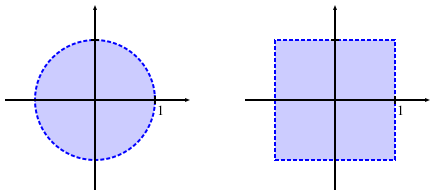
\includegraphics[width=\linewidth]{external/Equivalence.pdf}
\end{image}%
\tcblower
\end{figureptx}%
\end{sectionptx}
%
%
\typeout{************************************************}
\typeout{Section  Topological Equivalence}
\typeout{************************************************}
%
\begin{sectionptx}{Section}{Topological Equivalence}{}{Topological Equivalence}{}{}{section-sec_top_equiv}
When we can deform one set into another without poking holes in the set, we consider the two sets to be equivalent from a topological perspective. Such a deformation \(f\) has to be a bijection to ensure that the two sets contain the same number of elements, continuous so that the inverse images of open sets are open, and \(f^{-1}\) must be continuous so images of open sets are open. Such a function provides a one-to-one correspondence between open sets in the two spaces. This leads to the next definition.%
\begin{definition}{Definition}{}{definition-def_MS_topological_equivalence}%
\index{topologically equivalent}%
Two topological spaces \((X,d_X)\) and \((Y,d_Y)\) are \terminology{topologically equivalent} if there is a continuous bijection \(f : X \to Y\) such that \(f^{-1}\) is also continuous.%
\end{definition}
Metric equivalence always implies topological equivalence (using the metric topologies), which is left for \hyperlink{exercise-ex_me_implies_te}{Exercise~{\xreffont 3}}. So metric equivalence is a stronger condition than topological equivalence.%
\par
The function \(f\) (or \(f^{-1}\)) in \hyperref[definition-def_MS_topological_equivalence]{Definition~{\xreffont\ref{definition-def_MS_topological_equivalence}}} is called a \terminology{homeomorphism}.%
\begin{definition}{Definition}{}{definition-def_Homeomorphism}%
\index{homeomorphism}%
Let \((X,\tau_X)\) and \((Y,\tau_Y)\) be topological spaces. A function \(f: X \to Y\) is a \terminology{homeomorphism} if \(f\) is a continuous bijection such that \(f^{-1}\) is also continuous.%
\end{definition}
\index{homeomorphic spaces} If there is a homeomorphism from \((X,\tau_X)\) to \((Y,\tau_Y)\) we say that the spaces \((X,\tau_X)\) to \((Y,\tau_Y)\) are \terminology{homeomorphic} topological spaces.%
\par
It can be difficult to show directly that two metric spaces are homeomorphic, but there are ways to make the process easier in metric spaces. If \(f\) is a homeomorphism from the metric space \((\R^2, d_E)\) to the metric space \((\R^2, d_M)\), the continuity of \(f\) ensures a smooth deformation from \(\R^2\) to \(\R^2\). In terms of the metrics, this means that distances cannot get distorted too much \textemdash{} in fact, the amount distances are distorted should be bounded. In other words, we might expect that there is a constant \(K\) so that \(d_E(x,y) \leq K d_M(f(x),
f(y))\) for any \(x, y \in \R^2\). The next theorem tells us that this is a sufficient condition for topological equivalence when we work in the same underlying space.%
\begin{theorem}{Theorem}{}{}{theorem-sec_top_equiv-i}%
Let \(X\) be a set on which two metrics \(d\) and \(d'\) are defined. If there exist positive constants \(K\) and \(K'\) so that%
\begin{align*}
d'(x,y) \amp \leq K d(x,y)\\
d(x,y) \amp \leq K' d'(x,y)
\end{align*}
for all \(x,y \in X\), then \((X,d)\) is topologically equivalent to \((X,d')\).%
\end{theorem}
\begin{proof}{Proof}{}{proof-sec_top_equiv-i-b}
Let \(X\) be a set on which two metrics \(d\) and \(d'\) are defined. Suppose there exist positive constants \(K\) and \(K'\) so that%
\begin{align*}
d'(x,y) \amp \leq K d(x,y)\\
d(x,y) \amp \leq K' d'(x,y)
\end{align*}
for all \(x,y \in X\). Let \(i_X : (X,d) \to (X,d')\) be the identity mapping. That is, \(i_X(x)=x\) for all \(x \in X\). We will prove that \(i_X\) is a homeomorphism. We know that \(i_X\) is a bijection, so we only need verify that \(i_X\) and \(i_X^{-1}\) are continuous. Let \(\epsilon \gt 0\) be given, and let \(a \in X\). Let \(\delta = \frac{\epsilon}{K}\). Suppose \(x \in X\) so that \(d(x,a) \lt  \delta\). Then%
\begin{equation*}
d'(i_X(x), i_X(a)) = d'(x,a) \leq Kd(x,a) \lt  K\delta = K\left(\frac{\epsilon}{K}\right) = \epsilon\text{.}
\end{equation*}
%
\par
Thus, \(i_X\) is continuous. The same argument shows that \(i_X^{-1}\) is also continuous. Therefore, \(i_X\) is a homeomorphism between \((X,d)\) and \((X,d')\).%
\end{proof}
\begin{activity}{Activity}{}{activity-sec_top_equiv-j}%
\begin{enumerate}[font=\bfseries,label=(\alph*),ref=\alph*]%
\item{}Are \((\R^2,d_T)\) and \((\R^2, d_M)\) topologically equivalent? Explain.%
\item{}Are \((\R^2,d_E)\) and \((\R^2, d_T)\) topologically equivalent? Explain.%
\item{}Do you expect that \((\R^2,d_E)\) and \((\R^2, d_M)\) are topologically equivalent. Explain without doing any calculations or comparisons.%
\end{enumerate}%
\end{activity}%
\end{sectionptx}
%
%
\typeout{************************************************}
\typeout{Section  Relations}
\typeout{************************************************}
%
\begin{sectionptx}{Section}{Relations}{}{Relations}{}{}{section-sec_relations}
We use the word ``equivalent'' deliberately when talking about metric or topological equivalence. Recall that equivalence is a word used with relations, and that a relation is a way to compare two elements from a set. We are familiar with many relations on sets, ``\(\lt\)'', ``\(=\)'', ``\(\geq\)'' on the integers, for example.%
\begin{definition}{Definition}{}{definition-sec_relations-c}%
\index{relation}%
A \terminology{relation} on a set \(S\) is a subset \(R\) of \(S \times S\).%
\end{definition}
For example, the subset \(R = \{(a,a) \mid a \in \Z \}\) of \(\Z \times \Z\) is the relation we call equals. If \(R\) is a relation on a set \(S\), we usually suppress the set notation and write \(a \sim b\) if \((a,b) \in R\) and say that \(a\) is related to \(b\). In this case we often refer to \(\sim\) as the relation instead of the set \(R\). Sometimes we use familiar symbols for special relations. For example, we write \(a = b\) if \((a,b) \in R = \{(a,a) \mid a \in \Z \}\).%
\par
When discussing relations, there are three specific properties that we consider.%
\begin{itemize}[label=\textbullet]
\item{}A relation \(\sim\) on a set \(S\) is \terminology{reflexive} if \(a \sim a\) for all \(a \in S\).%
\item{}A relation \(\sim\) on a set \(S\) is \terminology{symmetric} if whenever \(a \sim b\) in \(S\) we also have \(b \sim a\).%
\item{}A relation \(\sim\) on a set \(S\) is \terminology{transitive} if whenever \(a \sim b\) and \(b \sim c\) in \(S\) we also have \(a \sim c\).%
\end{itemize}
%
\par
When we use the word ``equivalence'', we are referring to an equivalence relation.%
\begin{definition}{Definition}{}{definition-sec_relations-g}%
\index{equivalence relation}%
An \terminology{equivalence relation} is a relation on a set that is reflexive, symmetric, and transitive.%
\end{definition}
\begin{activity}{Activity}{}{activity-sec_relations-h}%
\begin{enumerate}[font=\bfseries,label=(\alph*),ref=\alph*]%
\item{}Explain why metric equivalence is an equivalence relation.%
\item{}Explain why topological equivalence is an equivalence relation.%
\end{enumerate}%
\end{activity}%
Equivalence relations are important because an equivalence relation on a set \(S\) partitions the set into a disjoint union of equivalence classes. Since topological equivalence is an equivalence relation, we can treat the spaces that are topologically equivalent to each other as being essentially the same space from a topological perspective. Under the relation of homeomorphism we call the equivalence classes \terminology{homeomorphism} classes.%
\end{sectionptx}
%
%
\typeout{************************************************}
\typeout{Section  Topological Invariants}
\typeout{************************************************}
%
\begin{sectionptx}{Section}{Topological Invariants}{}{Topological Invariants}{}{}{section-sec_top_invar}
Homeomorphic topological spaces are essentially the same from a topological perspective, and they share many properties, but not all. The properties they share are called \terminology{topological invariants} or \terminology{topological properties}.%
\begin{definition}{Definition}{}{definition-sec_top_invar-c}%
\index{topological property}%
\index{topological invariant}%
A property of a topological space \(X\) is a \terminology{topological property} (or \terminology{topological invariant} ) if every topological space homeomorphic to \(X\) has the same property.%
\end{definition}
\begin{activity}{Activity}{}{activity-sec_top_invar-d}%
Which of the following are topological invariants? That is for topological spaces \((X, \tau_X)\) and \((Y, \tau_Y)\), if \(X\) and \(Y\) are homeomorphic space and \(X\) has the property, does it follow that \(Y\) must also have that property?%
\begin{enumerate}[font=\bfseries,label=(\alph*),ref=\alph*]%
\item{}\(X\) has the indiscrete topology%
\item{}\(X\) has the discrete topology%
\item{}\(X\) has the finite complement topology%
\item{}\(X\) contains the number 2%
\item{}\(X\) contains exactly 13 elements%
\end{enumerate}%
\end{activity}%
\end{sectionptx}
%
%
\typeout{************************************************}
\typeout{Section  Summary}
\typeout{************************************************}
%
\begin{sectionptx}{Section}{Summary}{}{Summary}{}{}{section-sec_cont_top_summ}
Important ideas that we discussed in this section include the following.%
\begin{itemize}[label=\textbullet]
\item{}A function \(f\) from a topological space \(X\) to a topological space \(Y\) is continuous if \(f^{-1}(O)\) is open in \(X\) whenever \(O\) is open in \(Y\).%
\item{}Two metric spaces \((X,d_X)\) and \((Y,d_Y)\) are metrically equivalent if there is a bijection \(f : X \to Y\) such that%
\begin{align*}
d_X(x,y) \amp = d_Y(f(x),f(y))\\
d_Y(u,v) \amp = d_X(f^{-1}(u), f^{-1}(v))
\end{align*}
for all \(x,y \in X\) and \(u,v \in Y\). That is, \(X\) and \(Y\) are metrically equivalent if there is a isometry \(f\) from \(X\) to \(Y\) such that \(f^{-1}\) is also an isometry. Topological equivalence is a less stringent condition. Two topological spaces \(X\) and \(Y\) are topologically equivalent if there is a continuous function \(f\) from \(X\) to \(Y\) such that \(f^{-1}\) is also continuous. That is, \(X\) and \(Y\) are topologically equivalent if there is a homeomorphism between \(X\) to \(Y\).%
\item{}A homeomorphism between topological spaces \(X\) and \(Y\) is a continuous function \(f\) from \(X\) to \(Y\) such that \(f^{-1}\) is also continuous. Two topological spaces \(X\) and \(Y\) are homeomorphic if there is a homeomorphism \(f : X \to Y\).%
\item{}A topological invariant is any property that topological space \(X\) has that must also be a property of any topological space homeomorphic to \(X\). We can sometimes use topological invariants to determine if two topological spaces are not homeomorphic.%
\end{itemize}
%
\end{sectionptx}
%
%
\typeout{************************************************}
\typeout{Exercises  Exercises}
\typeout{************************************************}
%
\begin{exercises-section}{Exercises}{Exercises}{}{Exercises}{}{}{exercises-sec_cont_top_exer}
\begin{divisionexercise}{1}{}{}{exercise-ex_isometry_reverse}%
Let \((X,d_X)\) and \((Y,d_Y)\) be metrically equivalent metric spaces, and let \(f:X \to Y\) be a bijection such that%
\begin{equation*}
d_X(x,y) = d_Y(f(x),f(y))
\end{equation*}
for all \(x,y \in X\). Prove that%
\begin{equation*}
d_Y(u,v) = d_X(f^{-1}(u), f^{-1}(v))
\end{equation*}
for all \(u\) and \(v\) in \(Y\).%
\end{divisionexercise}%
\begin{divisionexercise}{2}{}{}{exercise-sec_cont_top_exer-b}%
Let \((X, \tau_X)\) and \((Y, \tau_Y)\) be topological spaces, and let \(f : X \to Y\) be a homeomorphism. Let \(A\) be a subset of \(X\).%
\begin{enumerate}[font=\bfseries,label=(\alph*),ref=\alph*]%
\item{}If \(x\) is a limit point of \(A\), must \(f(x)\) be a limit point of \(f(A)\)? Prove your answer.%
\item{}If \(x\) is an interior point of \(A\), must \(f(x)\) be an interior point of \(f(A)\)? Prove your answer.%
\item{}If \(x\) is a boundary point of \(A\), must \(f(x)\) be a boundary point of \(f(A)\)? Prove your answer.%
\end{enumerate}%
\end{divisionexercise}%
\begin{divisionexercise}{3}{}{}{exercise-ex_me_implies_te}%
Let \((X, d_X)\) and \((Y, d_Y)\) be metrically equivalent metric spaces. Show that \(X\) and \(Y\) are topologically equivalent using the metric topologies.%
\end{divisionexercise}%
\begin{divisionexercise}{4}{}{}{exercise-ex_closed_sets_continuity_TS}%
Prove \hyperref[theorem-thm_closed_sets_continuity_TS]{Theorem~{\xreffont\ref{theorem-thm_closed_sets_continuity_TS}}} that if \((X,\tau_X)\) and \((Y, \tau_Y)\) are topological spaces, and \(f: X \to Y\) is a function, then \(f\) is continuous if and only if \(f^{-1}(C)\) is a closed set in \(X\) whenever \(C\) is a closed set in \(Y\).%
\end{divisionexercise}%
\begin{divisionexercise}{5}{}{}{exercise-sec_cont_top_exer-e}%
Let \((X, \tau_X)\), \((Y, \tau_Y)\), and \((Z, \tau_Z)\) be topological spaces.%
\begin{enumerate}[font=\bfseries,label=(\alph*),ref=\alph*]%
\item{}Let \(f: X \to Y\) and \(g : Y \to Z\) be continuous functions. Prove that \(g \circ f : X \to Z\) is a continuous function.%
\par\smallskip%
\noindent\textbf{\blocktitlefont Hint}.\hypertarget{hint-sec_cont_top_exer-e-b-b}{}\quad{}\hyperlink{exercise-ex_inverse_composite_sets}{Exercise~{\xreffont 9}} could be helpful here.%
\item{}Let \(f: (X, \tau_X) \to (Y, \tau_Y)\) be a homeomorphism. Let \(h\) be a function from \((Y, \tau_Y)\) to \((Z, \tau_Z)\) and let \(k\) be a function from \((Z, \tau_Z)\) to \((X, \tau_X)\).%
\begin{enumerate}[font=\bfseries,label=(\roman*),ref=\theenumi.\roman*]%
\item{}Prove that \(h\) is continuous if and only if \(h \circ f\) is continuous.%
\item{}Prove that \(k\) is continuous if and only if \(f \circ k\) is continuous.%
\end{enumerate}%
\end{enumerate}%
\end{divisionexercise}%
\begin{divisionexercise}{6}{}{}{exercise-sec_cont_top_exer-f}%
Let \(X = \{a,b,c,d\}\) with topology \(\tau = \{\emptyset, \{a\}, \{b\}, \{a,b\}, \{b,d\}, \{a,b,d\}, X\}\).%
\begin{enumerate}[font=\bfseries,label=(\alph*),ref=\alph*]%
\item{}Find a function \(f: X \to X\) that is continuous at exactly one point, or show that no such function exists.%
\item{}Find a function \(f: X \to X\) that is continuous at exactly two points, or show that no such function exists.%
\item{}Find a function \(f: X \to X\) that is continuous at exactly three points, or show that no such function exists.%
\end{enumerate}%
\end{divisionexercise}%
\begin{divisionexercise}{7}{}{}{exercise-sec_cont_top_exer-g}%
Consider \(\R\) and \(\R^2\) equipped with the Euclidean topology. Let \(f : \R \to \R\) be a function and let%
\begin{equation*}
\Gamma_f = \{(x,f(x)) \mid x \in \R\}
\end{equation*}
be the graph of \(f\). Note that \(\Gamma_f\) is a subspace of \(\R^2\) and is a topological space using the subspace topology.%
\begin{enumerate}[font=\bfseries,label=(\alph*),ref=\alph*]%
\item{}Show that if \(f\) is a continuous function, then \(\Gamma_f\) is homeomorphic to \(\R\).%
\item{}If we remove the condition that \(f\) is continuous, must it still be the case that \(\Gamma_f\) is homeomorphic to \(\R\)? Prove your conjecture.%
\end{enumerate}%
\end{divisionexercise}%
\begin{divisionexercise}{8}{}{}{exercise-sec_cont_top_exer-h}%
Let \(X\) be a nonempty set and let \(p\) be a fixed element in \(X\). Let \(\tau_p\) be the particular point topology and \(\tau_{\overline{p}}\) the excluded point topology on \(X\). That is%
\begin{itemize}[label=\textbullet]
\item{}\(\tau_{p}\) is the collection of subsets of \(X\) consisting of \(\emptyset\), \(X\), and all of the subsets of \(X\) that contain \(p\).%
\item{}\(\tau_{\overline{p}}\) is the collection of subsets of \(X\) consisting of \(\emptyset\), \(X\), and all of the subsets of \(X\) that do not contain \(p\).%
\end{itemize}
That the particular point and excluded point topologies are topologies is the subject of \hyperlink{exercise-ex_particular_point_topology}{Exercise~{\xreffont 9}} and \hyperlink{exercise-ex_excluded_point_topology}{Exercise~{\xreffont 10}}.%
\begin{enumerate}[font=\bfseries,label=(\alph*),ref=\alph*]%
\item{}Let \(p\) be a fixed point in \(\R\). Is the identity function \(i: \R \to \R\) defined by \(i(x) = x\) for all \(x \in \R\) a homeomorphism from \((\R, \tau_p)\) to \((\R, \tau_{\overline{p}})\)? Prove your answer.%
\item{}Is \((\R, \tau_{p})\) homeomorphic to \((\R, \tau_{\overline{p}})\) with the specific point \(p=0\)? Prove your answer.%
\end{enumerate}%
\end{divisionexercise}%
\begin{divisionexercise}{9}{}{}{exercise-sec_cont_top_exer-i}%
A topological space \(X\) is \terminology{embedded} in a topological space \(Y\) if there is a homeomorphism from \(X\) to some subspace of \(Y\). The homeomorphism is called an \terminology{embedding}.%
\begin{enumerate}[font=\bfseries,label=(\alph*),ref=\alph*]%
\item{}Show that if \(X\) is the open interval \((0,1)\) with the Euclidean metric topology, then \(X\) can be embedded in the topological space \(\R\) with the Euclidean metric topology.%
\item{}Show that there exist non-homeomorphic topological spaces \(A\) and \(B\) for which \(A\) can be embedded in \(B\) and \(B\) can be embedded in \(A\).%
\end{enumerate}%
\end{divisionexercise}%
\begin{divisionexercise}{10}{}{}{exercise-sec_cont_top_exer-j}%
Let \(X = \{a,b\}\) be a two element set.%
\begin{enumerate}[font=\bfseries,label=(\alph*),ref=\alph*]%
\item{}Find all of the distinct topologies on \(X\). Be sure to explain how you know you have identified all of the topologies.%
\item{}Determine the distinct homeomorphism classes of topological spaces on two elements. Justify your response.%
\end{enumerate}%
\end{divisionexercise}%
\begin{divisionexercise}{11}{}{}{exercise-sec_cont_top_exer-k}%
Let \(X = \{a,b,c\}\). There are 29 distinct topologies on \(X\), shown below. Determine the number of distinct homeomorphism classes for these 29 topologies and identify the elements of each homeomorphism class. Justify your answers.%
\begin{enumerate}[font=\bfseries,label=(\alph*),ref=\alph*]%
\item{}\(\{\emptyset, X\}\)%
\item{}\(\{\emptyset, \{a,b\}, X\}\)%
\item{}\(\{\emptyset, \{a,c\}, X\}\)%
\item{}\(\{\emptyset, \{b,c\}, X\}\)%
\item{}\(\{\emptyset, \{a\}, X\}\)%
\item{}\(\{\emptyset, \{b\}, X\}\)%
\item{}\(\{\emptyset, \{c\}, X\}\)%
\item{}\(\{\emptyset, \{a\}, \{a,b\}, X\}\)%
\item{}\(\{\emptyset, \{a\}, \{a,c\}, X\}\)%
\item{}\(\{\emptyset, \{a\}, \{b,c\}, X\}\)%
\item{}\(\{\emptyset, \{b\}, \{a,b\}, X\}\)%
\item{}\(\{\emptyset, \{b\}, \{a,c\}, X\}\)%
\item{}\(\{\emptyset, \{b\}, \{b,c\}, X\}\)%
\item{}\(\{\emptyset, \{c\}, \{a,b\}, X\}\)%
\item{}\(\{\emptyset, \{c\}, \{a,c\}, X\}\)%
\item{}\(\{\emptyset, \{c\}, \{b,c\}, X\}\)%
\item{}\(\{\emptyset, \{a\}, \{a,b\}, \{a,c\}, X\}\)%
\item{}\(\{\emptyset, \{b\}, \{a,b\}, \{b,c\}, X\}\)%
\item{}\(\{\emptyset, \{c\}, \{a,c\}, \{b,c\}, X\}\)%
\item{}\(\{\emptyset, \{a\}, \{b\}, \{a,b\}, X\}\)%
\item{}\(\{\emptyset, \{a\}, \{c\}, \{a,c\}, X\}\)%
\item{}\(\{\emptyset, \{b\}, \{c\}, \{b,c\}, X\}\)%
\item{}\(\{\emptyset, \{a\}, \{b\}, \{a,b\}, \{a,c\}, X\}\)%
\item{}\(\{\emptyset, \{a\}, \{b\}, \{a,b\}, \{b,c\}, X\}\)%
\item{}\(\{\emptyset, \{a\}, \{c\}, \{a,c\}, \{a,b\}, X\}\)%
\item{}\(\{\emptyset, \{a\}, \{c\}, \{a,c\}, \{b,c\}, X\}\)%
\item{}\(\{\emptyset, \{b\}, \{c\}, \{b,c\}, \{a,b\}, X\}\)%
\item{}\(\{\emptyset, \{b\}, \{c\}, \{b,c\}, \{a,c\}, X\}\)%
\item{}the discrete topology%
\end{enumerate}%
\end{divisionexercise}%
\begin{divisionexercise}{12}{}{}{exercise-sec_cont_top_exer-l}%
Show that property \(T_i\) is a topological property for each \(i\). (See \hyperref[chapter-chap_Closed_sets_topology]{Chapter~{\xreffont\ref{chapter-chap_Closed_sets_topology}}} for definitions of the separation axioms.)%
\end{divisionexercise}%
\begin{divisionexercise}{13}{}{}{exercise-sec_cont_top_exer-m}%
For each of the following, answer true if the statement is always true. If the statement is only sometimes true or never true, answer false and provide a concrete example to illustrate that the statement is false. If a statement is true, explain why.%
\begin{enumerate}[font=\bfseries,label=(\alph*),ref=\alph*]%
\item{}If \(f : X \to Y\) is a continuous function between topological spaces \(X\) and \(Y\), then for every open subset \(U\) of \(X\), \(f(U)\) is open in \(Y\).%
\item{}If \(\tau_{FC}\) is the finite complement topology, then \(f(x) = x^2\) mapping \((\R, \tau_{FC})\) to \((\R, \tau_{FC})\) is continuous.%
\item{}If \(f : X \to Y\) is a bijective function between topological spaces \(X\) and \(Y\), and for every open subset \(U\) of \(X\), \(f(U)\) is open in \(Y\), then \(f\) is a homeomorphism.%
\item{}If \(X\) and \(Y\) are topological space with the discrete topologies, and if \(f: X \to Y\) is a bijection, then the spaces \(X\) and \(Y\) are homeomorphic.%
\item{}Let \(S\) be a set and let \(R_1\) and \(R_2\) be equivalence relations on \(S\). Then \(R = R_1 \cap R_2\) is also an equivalence relation on \(S\).%
\item{}Let \(S\) be a set and let \(R_1\) and \(R_2\) be equivalence relations on \(S\). Then \(R = R_1 \cup R_2\) is also an equivalence relation on \(S\).%
\end{enumerate}%
\end{divisionexercise}%
\end{exercises-section}
\end{chapterptx}
 %
%
\typeout{************************************************}
\typeout{Chapter 15 Subspaces}
\typeout{************************************************}
%
\begin{chapterptx}{Chapter}{Subspaces}{}{Subspaces}{}{}{chapter-chap_subspaces}
\renewcommand*{\chaptername}{Chapter}
\begin{objectives}{Focus Questions}{objectives-chap_subspaces-b}
%
\begin{itemize}[label=\textbullet]
\item{}What is a subspace of a topological space?%
\item{}How do we define the subspace topology?%
\item{}What are relatively open and closed sets?%
\item{}To what kind of spaces is \(\R\) with the standard topology homeomorphic?%
\end{itemize}
\end{objectives}
%
%
\typeout{************************************************}
\typeout{Section  Introduction}
\typeout{************************************************}
%
\begin{sectionptx}{Section}{Introduction}{}{Introduction}{}{}{section-sec_sub}
We have seen that a subset \(A\) of a metric space \((X,d_X)\) is a subspace of \(X\) using the restriction of the metric \(d_X\) to \(A\). We do not have a metric in general topological spaces, so that approach can't be duplicated. But, we proved that the open sets in a subspace \(A\) of a metric space \((X,d_X)\) are exactly the intersections of open sets in \(X\) with \(A\). That idea can be transferred to topological spaces.%
\par
To make a subspace \(A\) of a topological space \((X,\tau)\) into a topological space, we need to define a topology on \(A\).%
\begin{exploration}{Preview Activity}{}{exploration-sec_sub-d}%
Let \((X, \tau)\) be a topological space and \(A\) a nonempty subset of \(X\). It is reasonable to use the open sets in \(X\) to define open sets in \(A\). More specifically, we might consider a subset \(O_A\) of \(A\) to be open in \(A\) if \(O_A\) is the intersection of \(A\) with some open set in \(X\), as illustrated in \hyperref[figure-F_Subspace_open]{Figure~{\xreffont\ref{figure-F_Subspace_open}}}. With this in mind we define \(\tau_A\) as%
\begin{equation*}
\tau_A = \{O \cap A \mid O \in \tau\}\text{.}
\end{equation*}
%
\begin{figureptx}{Figure}{A potentially open subset in a subspace.}{figure-F_Subspace_open}{}%
\begin{image}{0.25}{0.5}{0.25}{}%
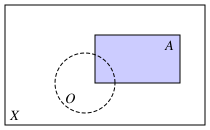
\includegraphics[width=\linewidth]{external/Subspace_open.pdf}
\end{image}%
\tcblower
\end{figureptx}%
\begin{enumerate}[font=\bfseries,label=(\alph*),ref=\alph*]%
\item\label{task-act_TS_subspace}Show that \(\tau_A\) is a topology on \(A\). The result of item (1) is that any subset of a topological space \((X,\tau)\) is also a topological space with topology \(\tau_A\).%
\begin{definition}{Definition}{}{definition-def_TS_subspace}%
\index{subspace of a topological space}%
Let \((X,\tau)\) be a topological space. A \terminology{subspace} of \((X,\tau)\) is a nonempty subset \(A\) of \(X\) together with the topology%
\begin{equation*}
\tau_A = \{O \cap A \mid O \in \tau\}\text{.}
\end{equation*}
%
\end{definition}
\item{}For each of the following, \(X\) is a topological space and \(\tau\) is a topology on \(X\).%
\begin{enumerate}[font=\bfseries,label=(\roman*),ref=\theenumi.\roman*]%
\item{}Let \(X= \{a,b,c,d\}\) and \(\tau = \{\emptyset, \{a\}, \{b\}, \{a,b\}, X \}\). Consider the subset \(A=\{b,c\}\) and list the open sets in the subspace topology \(\tau_A\). Now consider \(Z = \{a,b\}\). What is the name of the subspace topology \(\tau_Z\) on this subset of \(X\)?%
\item{}Consider \(X=\R\) with \(\tau\) the indiscrete topology. What are the open sets in the subspace topology on \([1,2]\)? Now generalize to any nonempty set in the indiscrete topology.%
\item{}Let \(X = \{a,b,c,d,e,f,g,h,i\}\) with \(\tau\) the discrete topology. What are the open sets in the subspace topology on \(\{a,b,d\}\). Now generalize to any nonempty set in the discrete topology.%
\item{}Let \(X= \{a,b,c,d,e,f\}\) with \(\tau = \{\emptyset,\{a\}, \{c,d\}, \{a,c,d\}, \{b,c,d,e,f\}, X\}\). What are the open sets in the subspace \(A = \{a, b, e\}\)? Is every open set in \(A\) an open set in \(X\)? Explain.%
\item{}Let \(X=\Z\) with \(\tau = \tau_{FC}\) the finite complement topology. What are the open sets in the subspace topology on \(A = \{0,19, 37, 5284\}\)? Can you generalize this to the subspace topology on any finite subset of \(\Z\)?%
\item{}Let \(X=\Z\) with \(\tau = \tau_{FC}\) the finite complement topology. What are the open sets in the subspace topology on the even integers? Can you generalize this to the subspace topology on any infinite subset of \(\Z\)?%
\end{enumerate}%
\end{enumerate}%
\end{exploration}%
\end{sectionptx}
%
%
\typeout{************************************************}
\typeout{Section  The Subspace Topology}
\typeout{************************************************}
%
\begin{sectionptx}{Section}{The Subspace Topology}{}{The Subspace Topology}{}{}{section-sec_subspace_top}
\index{subspace topology}%
\index{induced topology}%
\index{relative topology}%
\index{relatively open set}%
In our preview activity, we saw that the intersection of the open sets in a topological space \(X\) with any nonempty subset \(A\) of \(X\) forms a topology for \(A\). We then have \(A\) as a subspace of \(X\).%
\par
The topology \(\tau_A\) in \hyperref[definition-def_TS_subspace]{Definition~{\xreffont\ref{definition-def_TS_subspace}}} is called the \terminology{subspace topology}, the \terminology{induced topology}, or the \terminology{relative topology}. In our preview activity we saw that sets that are open in a subspace \(A\) of a topological space \(X\) need not be open in \(X\). So we call the sets in \(\tau_A\) \terminology{relatively open}.%
\par
Once we have defined relatively open sets, we can then consider how to define relatively closed sets.%
\begin{activity}{Activity}{}{activity-sec_subspace_top-i}%
Let \((X, \tau)\) be a topological space, and let \(A\) be a subset of \(X\).%
\begin{enumerate}[font=\bfseries,label=(\alph*),ref=\alph*]%
\item{}Recall that a subset of a topological space is closed if its complement is open. Given that \((A, \tau_A)\) is a topological space, how is a closed set in \(A\) defined? Such a set will be called \terminology{relatively closed}.%
\item{}Recall that a subset \(U\) of \(A\) is relatively open if and only if \(U = A \cap O\) for some open subset of \(X\). With this in mind, how might we expect a relatively closed set in \(A\) to be related to a closed set in \(X\)? State and prove a theorem for this result.%
\end{enumerate}%
\end{activity}%
\end{sectionptx}
%
%
\typeout{************************************************}
\typeout{Section  Bases for Subspaces}
\typeout{************************************************}
%
\begin{sectionptx}{Section}{Bases for Subspaces}{}{Bases for Subspaces}{}{}{section-sec_base_sub}
Recall that a basis \(\B\) for a topological space is a collection of sets that generate all of the open sets through unions. If we have a basis \(\B\) for a topological space \((X, \tau)\), and if \(A\) is a subspace of \(X\), we might ask if we can find a basis \(\B_A\) from \(\B\) in a natural way.%
\begin{activity}{Activity}{}{activity-sec_base_sub-c}%
Let \((X, \tau)\) be a topological space with basis \(\B\), and let \(A\) be a subspace of \(X\).%
\begin{enumerate}[font=\bfseries,label=(\alph*),ref=\alph*]%
\item{}There is a natural candidate to consider as a basis \(\B_A\) for \(A\). How do you think we should define the elements in \(\B_A\)?%
\item{}Recall that a set \(\B\) is a basis for a topological space \(X\) if%
\begin{enumerate}
\item{}For each \(x \in X\), there is a set in \(\B\) that contains \(x\).%
\item{}If \(x \in X\) is an element of \(B_1 \cap B_2\) for some \(B_1, B_2 \in B\), then there is a set \(B_3 \in \B\) such that \(x \in B_3 \subseteq B_1 \cap B_2\).%
\end{enumerate}
Show that your set from (a) is a basis for the induced topology on \(A\).%
\end{enumerate}%
\end{activity}%
\end{sectionptx}
%
%
\typeout{************************************************}
\typeout{Section  Open Intervals and \(\R\)}
\typeout{************************************************}
%
\begin{sectionptx}{Section}{Open Intervals and \(\R\)}{}{Open Intervals and \(\R\)}{}{}{section-sec_open_int_rn}
If we think of a homeomorphism as allowing us to stretch or bend a space, it is reasonable to think that we could stretch an open interval of the form \((a,b)\) infinitely in both directions without altering the nature of the open sets. That is, we should expect that \(\R\) with the standard topology is homeomorphic to \((a,b)\) with the subspace topology.%
\begin{activity}{Activity}{}{activity-sec_open_int_rn-c}%
Let \(a\) and \(b\) be real numbers with \(a \lt  b\). To show that \((\R, d_E)\) is homeomorphic to \((a,b)\), we need a continuous bijection from \(\R\) to \((a,b)\) whose inverse is also continuous.%
\begin{enumerate}[font=\bfseries,label=(\alph*),ref=\alph*]%
\item{}First we demonstrate that \((0,1)\) and \(\R\) are homeomorphic using the Euclidean metric topology. Let \(f : (0,1) \to \R\) be defined by%
\begin{equation*}
f(x) = \tan\left(\pi\left(x-\frac{1}{2}\right)\right)\text{.}
\end{equation*}
%
\begin{enumerate}[font=\bfseries,label=(\roman*),ref=\theenumi.\roman*]%
\item{}Explain why \(f\) maps \((0,1)\) to \(\R\).%
\item{}Explain why \(f\) is an injection.%
\item{}Explain why \(f\) is a surjection.%
\item{}Explain why \(f\) and \(f^{-1}\) are continuous.%
\par\smallskip%
\noindent\textbf{\blocktitlefont Hint}.\hypertarget{hint-sec_open_int_rn-c-b-e-b}{}\quad{}Use a result from calculus.%
\end{enumerate}%
\item{}The result of (a) is that \(\R\) and \((0,1)\) are homeomorphic spaces. To complete the argument that \(\R\) is homeomorphic to \((a,b)\), define a function \(g: (0,1) \to (a,b)\) and explain why your \(g\) is a homeomorphism.%
\end{enumerate}%
\end{activity}%
It is left to \hyperlink{exercise-ex_R_intervals}{Exercise~{\xreffont 4}} to show that \(\R\) is also homeomorphic to any interval of the form \((a,\infty)\) or \((-\infty,b)\). Later we will determine if \(\R\) is homeomorphic to intervals of the form \([a,b)\), \((a,b]\), \([a, \infty)\) or \((-\infty, b]\).%
\end{sectionptx}
%
%
\typeout{************************************************}
\typeout{Section  Summary}
\typeout{************************************************}
%
\begin{sectionptx}{Section}{Summary}{}{Summary}{}{}{section-sec_sub_summ}
Important ideas that we discussed in this section include the following.%
\begin{itemize}[label=\textbullet]
\item{}A subspace of a topological space is any nonempty subset of the topological space endowed with the subspace topology.%
\item{}An open subset in the subspace topology for a subset \(A\) of a topological space \(X\) is any set of the form \(O \cap A\), where \(O\) is an open set in \(X\).%
\item{}The relatively open sets are the open sets in a subspace topology. The relatively closed sets are complements of the relatively open sets in a subspace topology. That is, a relatively closed set in the subspace \(A\) of a topological space \(X\) are the sets of the form \(A \cap C\), where \(C\) is a closed set in \(X\).%
\item{}The topological space \(\R\) with the standard topology is homeomorphic to any open interval as well as open intervals of the form \((a,\infty)\) or \((-\infty,b)\) for any real numbers \(a\) and \(b\).%
\end{itemize}
%
\end{sectionptx}
%
%
\typeout{************************************************}
\typeout{Exercises  Exercises}
\typeout{************************************************}
%
\begin{exercises-section}{Exercises}{Exercises}{}{Exercises}{}{}{exercises-sec_sub_exer}
\begin{divisionexercise}{1}{}{}{exercise-sec_sub_exer-a}%
Let \(X\) and \(Y\) be topological spaces and \(f: X \to Y\) be a continuous function. If \(A\) is a subspace of \(X\), prove that \(f|_A : A \to Y\) is also continuous.%
\end{divisionexercise}%
\begin{divisionexercise}{2}{}{}{exercise-sec_sub_exer-b}%
Let \(X\) be a topological space, let \(A\) be a subspace of \(X\), and let \(B\) be a subspace of \(A\). Show that the subspace topology that \(B\) inherits from \(A\) is the same as the subspace topology that \(B\) inherits from \(X\).%
\end{divisionexercise}%
\begin{divisionexercise}{3}{}{}{exercise-sec_sub_exer-c}%
Let \(A\) be a subspace of a topological space \(X\) and let \(B\) be a subset of \(A\).%
\begin{enumerate}[font=\bfseries,label=(\alph*),ref=\alph*]%
\item{}Prove that a point \(x\) in \(A\) is a limit point of \(B\) in the subspace topology for \(A\) if and only if \(x\) is a limit point of \(B\) in the topology on \(X\).%
\item{}Prove that the closure of \(B\) in the subspace topology for \(A\) is equal to \(\overline{B} \cap A\), where \(\overline{B}\) is the closure of \(B\) in \(X\).%
\end{enumerate}%
\end{divisionexercise}%
\begin{divisionexercise}{4}{}{}{exercise-ex_R_intervals}%
Show that \(\R\) is homeomorphic, with the standard topology, to any interval of the form \((a,\infty)\) or \((-\infty,b)\).%
\end{divisionexercise}%
\begin{divisionexercise}{5}{}{}{exercise-sec_sub_exer-e}%
Let \(X\) be a topological space.%
\begin{enumerate}[font=\bfseries,label=(\alph*),ref=\alph*]%
\item{}Let \(O\) be an open subset of \(X\). Prove that a subset \(A\) of \(O\) is open in \(O\) if and only if \(A\) is open in \(X\).%
\item{}Let \(C\) be a closed subset of \(X\). Prove that a subset \(B\) of \(C\) is closed in \(C\) if and only if \(B\) is closed in \(X\).%
\end{enumerate}%
\end{divisionexercise}%
\begin{divisionexercise}{6}{}{}{exercise-sec_sub_exer-f}%
A property of a topological space is said to be hereditary if that property is inherited by every subspace. We state this more formally in the following definition.%
\begin{definition}{Definition}{}{definition-sec_sub_exer-f-a-b}%
\index{hereditary property}%
A property \(P\) of a topological space \(X\) is \terminology{hereditary} if every subspace of \(X\) also has property \(P\).%
\end{definition}
Show that properties \(T_1\), \(T_2\), and \(T_3\) are hereditary. (The separation axioms \(T_i\) are found in \hyperref[chapter-chap_Closed_sets_topology]{Chapter~{\xreffont\ref{chapter-chap_Closed_sets_topology}}}.) The fact that \(T_4\) is not hereditary is somewhat difficult. One example is the Tychonoff plank (which is normal) with the Deleted Tychonoff plank (which is not normal) as subspace. An interested reader can consult \pubtitle{Counterexamples in Topology (2nd ed.)}, Lynn Arthur Steen and J. Arthur Seebach, Jr., Dover Publications, 1978.%
\end{divisionexercise}%
\begin{divisionexercise}{7}{}{}{exercise-sec_sub_exer-g}%
Suppose that \(f : X \to Y\) is a homeomorphism from a topological space \(X\) to a topological space \(Y\). Let \(a \in X\). Must the subspace \(X' = X \setminus \{a\}\) of \(X\) be homeomorphic to the subspace \(Y' = Y \setminus \{f(a)\}\) of \(Y\)? Prove your conjecture.%
\end{divisionexercise}%
\begin{divisionexercise}{8}{}{}{exercise-sec_sub_exer-h}%
For each of the following, answer true if the statement is always true. If the statement is only sometimes true or never true, answer false and provide a concrete example to illustrate that the statement is false. If a statement is true, explain why.%
\begin{enumerate}[font=\bfseries,label=(\alph*),ref=\alph*]%
\item{}If \(X\) has the discrete topology, then every subspace of \(X\) has the discrete topology.%
\item{}If \(X\) is a topological space that does not have the discrete topology, then no subspace of \(X\) has the discrete topology.%
\item{}If \(f : X \to Y\) is a continuous function between topological spaces \(X\) and \(Y\), and \(X\) is Hausdorff, then the subspace \(f(X)\) of \(Y\) is Hausdorff.%
\item{}If \(A\) is a subspace of a topological space \(X\) and \(B\) is a subset of \(X\), then the closure of \(B \cap A\) in the subspace topology for \(A\) equals \(\overline{B} \cap A\), where \(\overline{B}\) is the closure of \(B\) in \(X\).%
\item{}If \(A\) is a subspace of a topological space \(X\) and \(C\) is a subset of \(X\), then the interior of \(C \cap A\) in the subspace topology for \(A\) equals \(\Int(C) \cap A\), where \(\Int(C)\) is the interior of \(C\) in \(X\).%
\end{enumerate}%
\end{divisionexercise}%
\end{exercises-section}
\end{chapterptx}
 %
%
\typeout{************************************************}
\typeout{Chapter 16 Quotient Spaces}
\typeout{************************************************}
%
\begin{chapterptx}{Chapter}{Quotient Spaces}{}{Quotient Spaces}{}{}{chapter-chap_quotients}
\renewcommand*{\chaptername}{Chapter}
\begin{objectives}{Focus Questions}{objectives-chap_quotients-b}
%
\begin{itemize}[label=\textbullet]
\item{}What is a quotient topology?%
\item{}What is a quotient space?%
\item{}What are two examples of familiar quotient spaces?%
\end{itemize}
\end{objectives}
%
%
\typeout{************************************************}
\typeout{Section  Introduction}
\typeout{************************************************}
%
\begin{sectionptx}{Section}{Introduction}{}{Introduction}{}{}{section-sec_quotients}
We are familiar with the word \terminology{quotient} when working with rational numbers. That is, the fraction \(\frac{1}{2}\) is the quotient of \(1\) by \(2\), and the set of rational numbers is the collection of all defined quotients of integers. The word quotient seems to have come from the latin word ``quotiens'', which can be translated as ``how often'' or ``how many times''. We can think of the fraction \(\frac{1}{2}\) as dividing a unit (\(1)\) into two pieces. So we often apply the word quotient to any kind of construction that divides a set into pieces. Another familiar quotient construction is the set \(\Z_n\), the set of quotients of integers after we divide by \(n\). Another way to think of \(\Z_n\) is as a quotient \(\Z/n\Z\), where \(n\Z\) is the set of multiples of \(n\) and two integers \(a\) and \(b\) are identified with each other (or are \terminology{equivalent}) if \(b-a \in n\Z\). This defines the relation of congruence module \(n\) on \(\Z\), and the elements of \(\Z/n\Z\) are the equivalence classes for this relation. We make similar constructions in many branches of mathematics by defining an equivalence relation on a set, and we then divide the set into pieces (the equivalence classes) and call the set of equivalence classes a \terminology{quotient space}. We explore the concept of quotient spaces of topological spaces in this section.%
\par
As an example, take the interval \(X = [0,1]\) in \(\R\) and bend it to be able to glue the endpoints together. The resulting object is a circle. By identifying the endpoints \(0\) and \(1\) of the interval, we are able to create a new topological space. We can view this gluing or identifying of points in the space \(X\) in a formal way that allows us to recognize the resulting space as a quotient space.%
\end{sectionptx}
%
%
\typeout{************************************************}
\typeout{Section  The Quotient Topology}
\typeout{************************************************}
%
\begin{sectionptx}{Section}{The Quotient Topology}{}{The Quotient Topology}{}{}{section-sec_quotient_top}
Given a topological space \(X\) and a surjection \(p\) from \(X\) to a set \(Y\), we can use the topology on \(X\) to define a topology on \(Y\). This topology on \(Y\) identifies points in \(X\) through the function \(p\). The resulting function on \(Y\) is called a \terminology{quotient} topology. The quotient topology gives us a way of creating a topological space which models gluing and collapsing parts of a topological space.%
\begin{exploration}{Preview Activity}{}{exploration-sec_quotient_top-c}%
Let \(X = \{1,2,3,4,5,6\}\) and let \(\tau = \{\emptyset, \{1,2\},\{4,6\}, \{1,2,4,6\},X\}\). Let \(Y = \{a,b,c,d\}\) and define \(p: X \to Y\) by%
\begin{equation*}
p(1) = b, \ p(2) = a, \ p(3) = c, \ p(4) = d, \ p(5) = c, \ \text{ and }  \ p(6) = a\text{.}
\end{equation*}
%
\par
Our goal in this activity is to define a topology on \(Y\) that is related to the topology on \(X\) via \(p\).%
\begin{enumerate}[font=\bfseries,label=(\alph*),ref=\alph*]%
\item{}We know the sets in \(X\) that are open. So let us consider the sets \(U\) in \(Y\) such that \(p^{-1}(U)\) is open in \(X\). Define \(\sigma\) to be this set. That is%
\begin{equation*}
\sigma = \{U \subseteq Y \mid p^{-1}(U) \in \tau\}\text{.}
\end{equation*}
Find all of the sets in \(\sigma\).%
\item{}Show that \(\sigma\) is a topology on \(Y\).%
\item{}Explain why \(p : (X, \tau) \to (Y, \sigma)\) is continuous.%
\item{}Show that \(\sigma\) is the largest topology on \(Y\) for which \(p\) is continuous. That is, if \(\sigma'\) is a topology on \(Y\) with \(\sigma \subsetneqq \sigma'\), then \(p: (X,\tau) \to (Y, \sigma')\) is not continuous.%
\end{enumerate}%
\end{exploration}%
\end{sectionptx}
%
%
\typeout{************************************************}
\typeout{Section  Quotient Spaces}
\typeout{************************************************}
%
\begin{sectionptx}{Section}{Quotient Spaces}{}{Quotient Spaces}{}{}{section-sec_quotient_space}
As we saw in our preview activity, if we have a surjection \(p\) from a topological space \((X,\tau)\) to a set \(Y\), we were able to define a topology on \(Y\) by making the open sets the sets \(U \subseteq Y\) such that \(p^{-1}(U)\) is open in \(X\). This is how we will create what is called the \terminology{quotient topology}. Before we can define the quotient topology, we need to know that this construction always makes a topology.%
\begin{activity}{Activity}{}{activity-act_quot_topology}%
Let \((X,\tau_X)\) be a topological space, let \(Y\) be a set, and let \(p: X \to Y\) be a surjection. Let%
\begin{equation*}
\tau_Y = \{U \subseteq Y \mid p^{-1}(U) \in \tau_X\}\text{.}
\end{equation*}
%
\begin{enumerate}[font=\bfseries,label=(\alph*),ref=\alph*]%
\item{}Why are \(\emptyset\) and \(Y\) in \(\tau_Y\)?%
\item{}Let \(\left\{U_{\beta}\right\}\) be a collection of sets in \(\tau_Y\) for \(\beta\) in some indexing set \(J\).%
\begin{enumerate}[font=\bfseries,label=(\roman*),ref=\theenumi.\roman*]%
\item{}Show that \(\bigcup_{\beta \in J} U_{\beta}\) is in \(\tau_Y\).%
\item{}If \(J\) is finite, show that \(\bigcap_{\beta \in J} U_{\beta}\) is in \(\tau_Y\).%
\end{enumerate}%
\item{}What conclusion can we draw about \(\tau_Y\)?%
\end{enumerate}%
\end{activity}%
\hyperref[activity-act_quot_topology]{Activity~{\xreffont\ref{activity-act_quot_topology}}} allows us to define the quotient topology.%
\begin{definition}{Definition}{}{definition-sec_quotient_space-e}%
\index{quotient topology}%
\index{quotient map}%
\index{quotient space}%
Let \((X,\tau_X)\) be a topological space, let \(Y\) be a set, and let \(p: X \to Y\) be a surjection.%
\begin{enumerate}
\item{}The \terminology{quotient topology} on \(Y\) is the set%
\begin{equation*}
\{U \subseteq Y \mid p^{-1}(U) \in \tau_X\}\text{.}
\end{equation*}
%
\item{}Any function \(p: X \to Y\) is a \terminology{quotient map} if \(p\) is surjective and for \(U \subseteq Y\), \(U\) is open in \(Y\) if and only if \(p^{-1}(U)\) is open in \(X\).%
\item{}If \(p: X \to Y\) is a quotient map, then the space \(Y\) is the \terminology{quotient space} of \(X\) determined by \(p\).%
\end{enumerate}
%
\end{definition}
\begin{activity}{Activity}{}{activity-sec_quotient_space-f}%
\begin{enumerate}[font=\bfseries,label=(\alph*),ref=\alph*]%
\item{}Let \(X=\R\) with standard topology, let \(Y=\{-1,0,1\}\), and define \(p:X \to Y\) by%
\begin{equation*}
p(x) = \begin{cases}1\amp \text{ if }  x>0 \\ 0 \amp \text{ if }  x=0 \\ -1 \amp \text{ if }  x\lt 0. \end{cases}
\end{equation*}
Find all of the open sets in the quotient topology.%
\item{}Let \(X=\R\) with standard topology, let \(Y=[0,1)\), and define \(p:X \to Y\) by%
\begin{equation*}
p(x) = x-\lfloor x\rfloor\text{,}
\end{equation*}
where \(\lfloor x\rfloor\) is the largest integer less than or equal to \(x\), (For example \(\lfloor 1.2 \rfloor = 1\), and so \(p(1.2) = 1.2 - 1 = 0.2\). The function defined by \(\lfloor x\rfloor\) is also called the \terminology{floor} function. Be careful, note that \(\lfloor -0.7 \rfloor = -1\).)  Determine the sets in the quotient topology.%
\begin{figureptx}{Figure}{The graph of \(p(x) = x - \lfloor x\rfloor\).}{figure-F_floor}{}%
\begin{image}{0.25}{0.5}{0.25}{}%
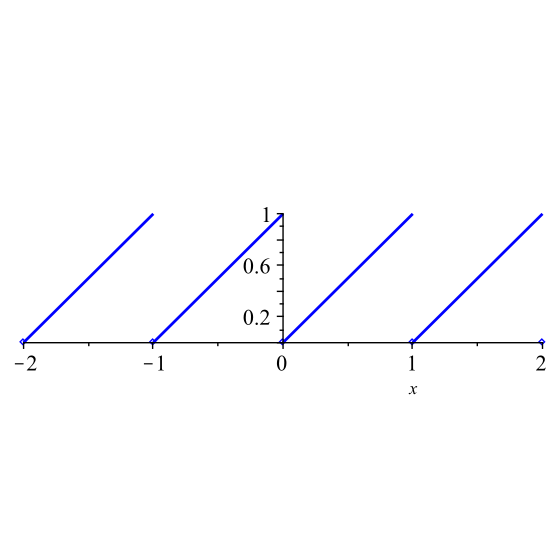
\includegraphics[width=\linewidth]{external/floor.pdf}
\end{image}%
\tcblower
\end{figureptx}%
\par\smallskip%
\noindent\textbf{\blocktitlefont Hint}.\hypertarget{hint-sec_quotient_space-f-b-b}{}\quad{}The graph of \(p\) on \([-2,2]\) is shown in \hyperref[figure-F_floor]{Figure~{\xreffont\ref{figure-F_floor}}}.%
\end{enumerate}%
\end{activity}%
Another perspective of the quotient topology utilizes the fact that any equivalence relation \(\sim\) on a set \(X\) partitions \(X\) into a union of disjoint equivalence classes \([x] = \{y \in X \mid y \sim x\}\). There is a natural surjection \(q\) from \(X\) to the space of equivalence classes given by \(q(x) = [x]\). We investigate this perspective in the next activity.%
\begin{activity}{Activity}{}{activity-act_quotient_er}%
Let \(X = \{a,b,c,d,e,f\}\) and let \(\tau = \{\emptyset, \{a\}, \{b\}, \{a, b\}, \{a, b, c\}, \{a, b, c, d\}, X\}\). Then \((X, \tau)\) is a topological space. Let \(A = \{a, b, c\}\) and \(B = \{d,e,f\}\). Define a relation \(\sim\) on \(X\) such that \(x \sim y\) if \(x\) and \(y\) are both in \(A\) or both in \(B\). Assume that \(\sim\) is an equivalence relation. The sets \(A\) and \(B\) are the equivalence classes for this relation. That is \(A = [a] = [b] = [c]\) and \(B = [d] = [e] = [f]\). Let \(X^* = \{A,B\}\). Then we can define \(p : X \to X^*\) by sending \(x \in X\) to the set to which it belongs. That is, \(p(x) = [x]\) for \(x \in X\), or%
\begin{equation*}
p(a) = A, p(b) = A, p(c) = A, p(d) = B, p(e) = B, \text{ and }  p(f) = B\text{.}
\end{equation*}
%
\par
Determine the sets in the quotient topology on \(X^*\).%
\end{activity}%
The partition of \(X\) in \hyperref[activity-act_quotient_er]{Activity~{\xreffont\ref{activity-act_quotient_er}}} into the disjoint union of sets \(A\) and \(B\) defines an equivalence relation on \(X\) where \(x \sim y\) if \(x\) and \(y\) are both in the same set \(A\) or \(B\). That is, \(a \sim b \sim c\) and \(d \sim e \sim f\). In this context, the sets \(A\) and \(B\) are equivalence classes \textemdash{} \(A = [a]\) and \(B = [d]\), where \([x]\) is the equivalence class of \(x\). This leads to a general construction.%
\par
\index{quotient space}\index{identification space} If \((X, \tau)\) is a topological space and \(\sim\) is an equivalence relation on \(X\), we can let \(X/\ssim\) be the set of distinct equivalence classes of \(X\) under \(\sim\). Then \(p: X \to X/\ssim\) defined by \(p(x) = [x]\) is a surjection and \(X/\ssim\) has the quotient topology. The space \(X/\ssim\) is called a \terminology{quotient space}. The space \(X/\ssim\) is also called an \terminology{identification} space because the equivalence relation identifies points in the set to be thought of as the same. This allows us to visualize quotient spaces as resulting from gluing or collapsing parts of the space \(X\).%
\begin{figureptx}{Figure}{A tube as the identification space \(X/\ssim\).}{figure-F_Quotient_tube}{}%
\begin{image}{0.05}{0.9}{0.05}{}%
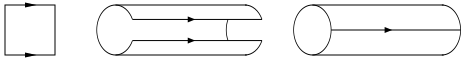
\includegraphics[width=\linewidth]{external/Cylinder_identification.pdf}
\end{image}%
\tcblower
\end{figureptx}%
\begin{example}{Example}{}{example-sec_quotient_space-l}%
Let \(I = [0,1]\) and let \(X = I \times I\) with standard topology. Define a relation \(\sim\) on \(X\) by \((x,y) \sim (x,y)\) if \(0 \lt y \lt 1\) and \(0 \leq x \leq 1\), \((x,0) \sim (x,1)\) if \(0 \leq x \leq 1\). It is straightforward to show that \(\sim\) is an equivalence relation. Let us consider what the identification space \(X/\ssim\) looks like. The space \(I \times I\) is the unit square as shown in \hyperref[figure-F_Quotient_tube]{Figure~{\xreffont\ref{figure-F_Quotient_tube}}}. All points in the interior of the square are identified only with themselves. However, the top side and bottom side are identified with each other in the same direction. Think of \(X\) as a piece of paper. We roll up the sides of the square to make the top and bottom sides coincide. The result is that \(X/\ssim\) is the cylinder as shown in \hyperref[figure-F_Quotient_tube]{Figure~{\xreffont\ref{figure-F_Quotient_tube}}}.%
\end{example}
\begin{activity}{Activity}{}{activity-sec_quotient_space-m}%
Quotient spaces can be difficult to describe. This activity presents a few more examples.%
\begin{enumerate}[font=\bfseries,label=(\alph*),ref=\alph*]%
\item{}Let \(X = [0, 1]\) with standard topology and define an equivalence relation \(\sim\) on \(X\) by \(0 \sim 1\) and \(x \sim x\) for all \(x\) not equal to \(0\) or \(1\). What does the quotient space \(X/\ssim\) look like?%
\begin{figureptx}{Figure}{From left to right: the identifications for parts (i), (ii), and (iii)}{figure-F_Quotients_activity}{}%
\begin{sidebyside}{3}{0}{0}{0}%
\begin{sbspanel}{0.333333333333333}%
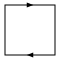
\includegraphics[width=\linewidth]{external/Mobius_identification.pdf}
\end{sbspanel}%
\begin{sbspanel}{0.333333333333333}%
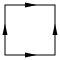
\includegraphics[width=\linewidth]{external/Torus_identification.pdf}
\end{sbspanel}%
\begin{sbspanel}{0.333333333333333}%
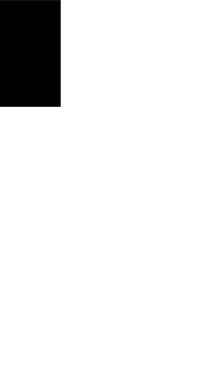
\includegraphics[width=\linewidth]{external/Quotient_sphere_1.pdf}
\end{sbspanel}%
\end{sidebyside}%
\tcblower
\end{figureptx}%
\par\smallskip%
\noindent\textbf{\blocktitlefont Hint}.\hypertarget{hint-sec_quotient_space-m-b-b}{}\quad{}Think about the relation \(\sim\) as gluing the points \(0\) and \(1\) together.%
\item{}Describe quotient spaces of \(X = I \times I\) with standard topology given by the following equivalence relations \(\sim\). Depictions of the identifications are shown in \hyperref[figure-F_Quotients_activity]{Figure~{\xreffont\ref{figure-F_Quotients_activity}}}. (Here \(I\) is the closed interval \([0,1]\).)%
\begin{enumerate}[font=\bfseries,label=(\roman*),ref=\theenumi.\roman*]%
\item{}\((x, y) \sim (x,y)\) if \(0 \lt y \lt 1\) and \(0 \leq x \leq 1\) and \((x,0) \sim (1-x,0)\) when \(0 \leq x \leq 1\).%
\item{}\((x, y) \sim (x,y)\) if \(0 \lt x \lt 1\) and \(0 \lt y \lt 1\), \((x,0) \sim (x,1)\) for \(0 \lt x \lt 1\), \((0,y) \sim (1,y)\) for \(0 \lt y \lt 1\), and \((0,0) \sim (0,1) \sim (1,0) \sim(1,1)\). (This space is called a Möbius strip.)%
\item{}\((x, y) \sim (x,y)\) if \(0 \lt x \lt 1\) and \(0 \lt y \lt 1\) and \((x,y) \sim (u,v)\) if \((x,y)\) and \((u,v)\) are boundary points.%
\end{enumerate}%
\end{enumerate}%
\end{activity}%
\index{Klein bottle} Many other interesting identification spaces can be made. For example, let \(X = I \times I\) and define \(\sim\) by \((x, y) \sim (x,y)\) if \(0 \lt x \lt 1\) and \(0 \lt y \lt 1\), \((0, y) \sim (1, y)\) for \(0 \lt y \lt 1\), \((x,0) \sim (1-x,1)\) for \(0 \lt x \lt 1\). This identification is illustrated in \hyperref[figure-F_Klein_bottle]{Figure~{\xreffont\ref{figure-F_Klein_bottle}}}. The resulting identification space \(X/\ssim\) is a Klein bottle. A nice illustration of this can be seen at \href{https://plus.maths.org/content/introducing-klein-bottle}{maths.org}\footnote{\nolinkurl{plus.maths.org/content/introducing-klein-bottle}\label{fn-sec_quotient_space-n-n}}.%
\begin{figureptx}{Figure}{Identifications for the Klein Bottle.}{figure-F_Klein_bottle}{}%
\begin{image}{0.3}{0.4}{0.3}{}%
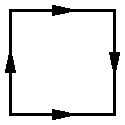
\includegraphics[width=\linewidth]{external/Klein_identification.pdf}
\end{image}%
\tcblower
\end{figureptx}%
\end{sectionptx}
%
%
\typeout{************************************************}
\typeout{Section  Identifying Quotient Spaces}
\typeout{************************************************}
%
\begin{sectionptx}{Section}{Identifying Quotient Spaces}{}{Identifying Quotient Spaces}{}{}{section-sec_find_quotient_space}
Suppose \(X\) is a topological space and \(Y\) is a set, and let \(p: X \to Y\) be a surjection. We can define a relation \(\sim_p\) on \(X\) by \(x \sim_p y\) if and only if \(p(x) = p(y)\). It is straightforward to show that \(\sim_p\) is an equivalence relation, the details are left for \hyperlink{exercise-ex_sim_p_relation}{Exercise~{\xreffont 1}}. From this we can see that our two approaches to defining the quotient topology and quotient spaces are really the same.%
\par
Oftentimes we have a topological space \(X\) and a relation \(\sim\) on \(X\), and we would like to have an effective way to be able to identify the quotient space \(X/\ssim\) as homeomorphic to some familiar topological space \(Y\). That is, we want to be able to show that there is a homeomorphism \(f\) from \(X/\ssim\) to \(Y\).%
\begin{example}{Example}{}{example-exp_R_Z_quotient}%
Consider the following situation. Let \(X = \R\) with the standard topology and define the relation \(\sim\) on \(\R\) by \(x \sim y\) if \(x - y \in \Z\). It is straightforward to show that \(\sim\) is an equivalence relation. By this equivalence relation, we have \(x-1 \sim x\) for every real number \(x\). This identifies \(\R\) with the interval \([0,1]\), where \(0\) and \(1\) are identified under the relation. So we might expect that \(\R/\ssim\) is homeomorphic to the circle \(S^1 = \{(x,y) \in \R^2 \mid x^2+y^2 = 1\}\) as a subspace of \(\R^2\) with the standard topology. Now the objective is to find a homeomorphism between \(S_1\) and \(\R/\ssim\). Since every point on the unit circle has the form \((\cos(t), \sin(t))\) for some real number \(t\), we might try defining \(f: (\R/\ssim) \to S^1\) by \(f([t]) = (\cos(t), \sin(t))\). However, we have that \(0 \sim 1\), which means that \([0] = [1]\), but \(f([0]) \neq f([1])\) and so \(f\) is not well-defined. Another option might be \(f([t]) = (\cos(2 \pi t), \sin(2 \pi t))\). In this case, if \(x \sim y\), then \(2 \pi x\) and \(2 \pi y\) differ by a multiple of \(2 \pi\) and so \(f([x]) = f([y])\). We could then show that \(f\) is a homeomorphism. We will continue this example shortly.%
\end{example}
The following theorem encapsulates the above example.%
\begin{theorem}{Theorem}{}{}{theorem-thm_quotient_1}%
Let \(X\) and \(Y\) be sets and let \(\sim\) be an equivalence relation on \(X\). Let \(f\) be a function from \(X\) to \(Y\) such that \(f(x_1) = f(x_2)\) whenever \(x_1 \sim x_2\) in \(X\). Let \(X/\ssim\) be the set of equivalence classes of \(X\) under the relation \(\sim\), and let \(p: X \to (X/\ssim)\) be the standard map defined by \(p(x) = [x]\). The function \(\overline{f}\) mapping \(X/\ssim\) to \(Y\) defined by \(\overline{f}([x]) = f(x)\) for every \(x \in X\) is the unique function that satisfies%
\begin{equation*}
f = \overline{f} \circ p\text{.}
\end{equation*}
%
\end{theorem}
\begin{activity}{Activity}{}{activity-sec_find_quotient_space-g}%
\hyperref[theorem-thm_quotient_1]{Theorem~{\xreffont\ref{theorem-thm_quotient_1}}} is a statement about sets and functions, and there is no topology involved. We prove the theorem in this activity. Use the conditions stated in \hyperref[theorem-thm_quotient_1]{Theorem~{\xreffont\ref{theorem-thm_quotient_1}}}.%
\begin{enumerate}[font=\bfseries,label=(\alph*),ref=\alph*]%
\item{}Show that \(\overline{f}\) is well-defined. That is, show that whenever \([x_1] = [x_2]\) in \(X/\ssim\), then \(\overline{f}([x_1]) =\overline{f}([x_2])\).%
\item{}Prove that \(f = \overline{f} \circ p\).%
\item{}Show that the uniqueness of \(\overline{f}\) comes from the equation \(f = \overline{f} \circ p\).%
\end{enumerate}%
\end{activity}%
Now we present a final result that can be very helpful when working with quotient spaces.%
\begin{theorem}{Theorem}{}{}{theorem-thm_quotient_2}%
Let \(X\) be a topological space and let \(\sim\) be an equivalence relation on \(X\). Consider the set \(X/\ssim\) to be a topological space with the quotient topology, and let \(p: X \to (X/\ssim)\) be the standard surjection defined by \(p(x) = [x]\). Let \(Y\) be a topological space with \(f: X \to Y\) a continuous function such that \(f(x_1) = f(x_2)\) whenever \(x_1 \sim x_2\) in \(X\). Then \(\overline{f} : (X/\ssim) \to Y\) defined by \(\overline{f}([x]) = f(x)\) is the unique continuous function satisfying \(f = \overline{f} \circ p\).%
\end{theorem}
\begin{proof}{Proof}{}{proof-thm_quotient_2-b}
The existence of \(\overline{f}\) as the unique function satisfying \(f = \overline{f} \circ p\) was established in \hyperref[theorem-thm_quotient_1]{Theorem~{\xreffont\ref{theorem-thm_quotient_1}}}. All that remains is to show that \(\overline{f}\) is continuous. Let \(O\) be an open set in \(Y\). Since \(f\) is continuous, we know that \(f^{-1}(O)\) is open in \(X\). If \(x_1 \in f^{-1}(O)\) and \(x_1 \sim x_2\), then \(x_2 \in f^{-1}(O)\) as well. Thus, we can write \(f^{-1}(O)\) as%
\begin{equation*}
f^{-1}(O) = \bigcup_{x \in f^{-1}(O)} [x]\text{.}
\end{equation*}
%
\par
That is, \(f^{-1}(O)\) is a union of equivalence classes. Now \(\overline{f}([x]) = f(x)\), so if \(x \in f^{-1}(O)\), then \([x] \in \overline{f}^{-1}(O)\). Thus,%
\begin{equation*}
f^{-1}(O) = \bigcup_{x \in f^{-1}(O)} [x] = \bigcup_{[x] \in \overline{f}^{-1}(O)} [x] = \overline{f}^{-1}(O)\text{.}
\end{equation*}
%
\par
We conclude that \(\overline{f}^{-1}(O)\) is open in \(X\) and \(\overline{f}\) is continuous.%
\end{proof}
Now we will see how to use \hyperref[theorem-thm_quotient_2]{Theorem~{\xreffont\ref{theorem-thm_quotient_2}}} to establish a homeomorphism from a quotient space of a given topological space to another topological space%
\begin{example}{Example}{}{example-sec_find_quotient_space-k}%
We return to the situation from \hyperref[example-exp_R_Z_quotient]{Example~{\xreffont\ref{example-exp_R_Z_quotient}}} with \(X = \R\) under the standard topology and equivalence relation \(\sim\) defined by \(x \sim y\) if \(x - y \in \Z\). We will use \hyperref[theorem-thm_quotient_2]{Theorem~{\xreffont\ref{theorem-thm_quotient_2}}} to show that \(\R/\ssim\) is homeomorphic to the circle \(Y = S^1\).%
\begin{figureptx}{Figure}{A basis element for \(S^1\).}{figure-F_S_1_basis}{}%
\begin{image}{0.25}{0.5}{0.25}{}%
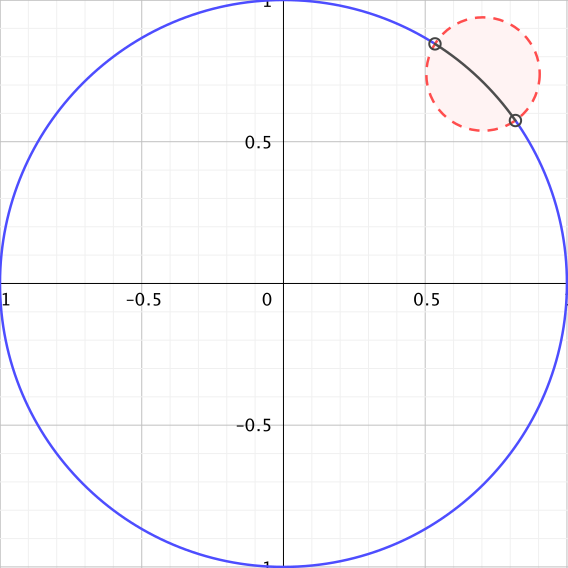
\includegraphics[width=\linewidth]{external/S_1_basis.pdf}
\end{image}%
\tcblower
\end{figureptx}%
%
\begin{descriptionlist}
\begin{dlimedium}{Step 1}{li-sec_find_quotient_space-k-a-c-a-a}%
Define a continuous surjection \(f: X \to Y\) that respects the relation. That is, we need to ensure that \(f(x_1) = f(x_2)\) whenever \(x_1 \sim x_2\) in \(X\). We saw earlier that the function \(f\) defined by \(f(t) = (\cos(2 \pi t), \sin(2 \pi t))\) respects the relation. Since every point on the unit circle is of the form \((\cos(\theta), \sin(\theta))\) for some real number \(\theta\), choosing \(t = \frac{\theta}{2 \pi}\) makes \(f(t) = (\cos(\theta), \sin(\theta))\) and \(f\) is a surjection. Now we need to demonstrate that \(f\) is continuous. A collection of basic open sets in \(S^1\) can be found by intersecting \(S^1\) with open balls in \(\R^2\) as illustrated in \hyperref[figure-F_S_1_basis]{Figure~{\xreffont\ref{figure-F_S_1_basis}}}. We can see that the basic open sets are arcs of the form \(\overparen{ab}\) for \(a\) and \(b\) in \(S^1\). Suppose \(a = (\cos(2 \pi A), \sin(2 \pi A))\) and \(b = (\cos(2 \pi B), \sin(2 \pi B))\) for angles \(A\) and \(B\). Then \(f^{-1}(\overparen{ab})\) is the union of intervals \((A+2\pi k, B+2 \pi k)\) for \(k \in \Z\). As a union of open intervals, we have that \(f^{-1}(\overparen{ab})\) is open in \(X\). We have now found a continuous surjection from \(X\) to \(Y\) that respects the relation.%
\end{dlimedium}%
\begin{dlimedium}{Step 2}{li-sec_find_quotient_space-k-a-c-a-b}%
Find a continuous function from \(X/\ssim\) to \(Y\). \hyperref[theorem-thm_quotient_2]{Theorem~{\xreffont\ref{theorem-thm_quotient_2}}} tells us that the function \(\overline{f} : (X/\ssim) \to Y\) defined by \(\overline{f}([t]) = f(t)\) is continuous. So \(\overline{f}\) is our candidate to be a homeomorphism.%
\end{dlimedium}%
\begin{dlimedium}{Step 3}{li-sec_find_quotient_space-k-a-c-a-c}%
Show that \(\overline{f}\) is a bijection. Let \(y \in Y\). The fact that \(f\) is a surjection means that there is a \(t \in \R\) such that \(f(t) = y\). It follows that \(\overline{f}([t]) = f(t) = y\) and \(\overline{f}\) is a surjection. To demonstrate that \(\overline{f}\) is an injection, suppose \(\overline{f}([s]) = \overline{f}([t])\) for some \(s,
t \in \R\). Then \((\cos(2 \pi s), \sin(2 \pi s)) = f(s) = f(t) = (\cos(2\pi t), \sin(2 \pi t))\). It must be the case then that \(2 \pi s\) and \(2 \pi t\) differ by a multiple of \(2 \pi\). That is, \(2 \pi s - 2 \pi t = 2 \pi k\) for some integer \(k\). From this we have \(s - t = k \in \Z\), and so \(s \sim t\). This makes \([s] = [t]\) and we conclude that \(\overline{f}\) is an injection.%
\end{dlimedium}%
\begin{dlimedium}{Step 4}{li-sec_find_quotient_space-k-a-c-a-d}%
Show that \(\overline{f}\) is a homeomorphism. At this point we already know that \(\overline{f}\) is a continuous bijection, so the only item that remains is to show that \(\overline{f}(\overline{O})\) is open whenever \(\overline{O}\) is open in \(X/\ssim\). Let \(p: X \to (X/\ssim)\) be the standard map. Let \(\overline{O}\) be a nonempty open set in \(X/\ssim\). Then \(O = p^{-1}(\overline{O})\) is open in \(X\). Thus, \(O\) is a union of open intervals. Let \((a,b)\) be an interval contained in \(O\). From the definition of \(f\) we have that \(f(a,b)\) is the open arc \(\overparen{f(a)f(b)}\), which is open in \(Y\). So \(f(O)\) is a union of open arcs in \(Y\), which makes \(f(O)\) open in \(Y\). Now \(f(O) = (\overline{f} \circ p)(O) = \overline{f}(p(O)) = \overline{f}(\overline{O})\), and \(\overline{f}(\overline{O})\) is open in \(Y\). We conclude that \(\overline{f}\) is a homeomorphism from \(X/\ssim\) to \(S^1\), and so \(S^1\) is a quotient space of \(\R\).%
\end{dlimedium}%
\end{descriptionlist}
%
\end{example}
\end{sectionptx}
%
%
\typeout{************************************************}
\typeout{Section  Summary}
\typeout{************************************************}
%
\begin{sectionptx}{Section}{Summary}{}{Summary}{}{}{section-sec_quotients_summ}
Important ideas that we discussed in this section include the following.%
\begin{itemize}[label=\textbullet]
\item{}Let \((X,\tau_X)\) be a topological space, let \(Y\) be a set, and let \(p: X \to Y\) be a surjection. The quotient topology on \(Y\) is the set%
\begin{equation*}
\{U \subseteq Y \mid p^{-1}(U) \in \tau_X\}\text{.}
\end{equation*}
%
\item{}The function \(p\) is a quotient topology as in the previous bullet is called a quotient map and the space \(Y\) is a quotient space.%
\item{}A circle, a Möbius strip, a torus, and a sphere can all be realized as quotient spaces.%
\end{itemize}
%
\end{sectionptx}
%
%
\typeout{************************************************}
\typeout{Exercises  Exercises}
\typeout{************************************************}
%
\begin{exercises-section}{Exercises}{Exercises}{}{Exercises}{}{}{exercises-sec_quotients_exer}
\begin{divisionexercise}{1}{}{}{exercise-ex_sim_p_relation}%
Let \(X\) be a topological space, \(Y\) a set, and \(p: X \to Y\) a surjection. Define the relation \(\sim_p\) on \(X\) by \(x \sim_p y\) if and only if \(p(x)=p(y)\). Prove that \(\sim_p\) is an equivalence relation.%
\end{divisionexercise}%
\begin{divisionexercise}{2}{}{}{exercise-sec_quotients_exer-c}%
Let \(X\) be the real numbers with the standard topology and let \(p: X \to \{a,b,c\}\) be defined by%
\begin{equation*}
p(x) = \begin{cases}a \amp \text{ if }  x \lt  0 \\ b \amp \text{ if }  x = 0 \\ c \amp \text{ if }  x \gt 0. \end{cases}
\end{equation*}
What is the quotient topology?%
\end{divisionexercise}%
\begin{divisionexercise}{3}{}{}{exercise-sec_quotients_exer-d}%
Define an equivalence relation \(\sim\) on \(\R^2\) by \((x_1,y_1) \sim (x_2,y_2)\) whenever \(x_2 - x_1 \in \Z\) and \(y_2 - y_1 \in \Z\).%
\begin{enumerate}[font=\bfseries,label=(\alph*),ref=\alph*]%
\item{}Prove that \(\sim\) is an equivalence relation on \(\R^2\).%
\item{}The quotient space is a familiar space. Find that space and explain why it is the quotient space.%
\end{enumerate}%
\end{divisionexercise}%
\begin{divisionexercise}{4}{}{}{exercise-sec_quotients_exer-e}%
Find an example of a continuous surjection that is not a quotient map.%
\end{divisionexercise}%
\begin{divisionexercise}{5}{}{}{exercise-sec_quotients_exer-f}%
Let \(X\) be a topological space and let \(A\) be a subspace of \(X\). Define a relation \(\sim\) on \(X\) whose equivalence classes are \(A\) and \(\{x\}\) if \(x \notin A\). In this case the quotient space is denoted as \(X/A\) (think of this space as obtained by crushing \(A\) to a point and leaving everything else alone). Describe each of the following quotient spaces.%
\begin{enumerate}[font=\bfseries,label=(\alph*),ref=\alph*]%
\item{}\(X\) is the closed interval \([0,1]\) in \(\R\) and \(A = \{0,1\}\)%
\item{}\(X = \{(x,y) \mid x^2+y^2 = 1\}\), \(A = \{(-1,0), (1,0)\}\)%
\item{}If \(X= \{(x,y) \mid x^2+y^2 \leq 1\}\) and \(A = \{(x,y) \mid x^2+y^2 = 1\}\)%
\end{enumerate}%
\end{divisionexercise}%
\begin{divisionexercise}{6}{}{}{exercise-sec_quotients_exer-g}%
Let \((X, \tau)\) be the topological space where \(X = \{1, 2, 3, 4\}\) and%
\begin{equation*}
\tau = \{\emptyset, \{1\}, \{2\}, \{1, 2\}, \{3, 4\}, \{2, 3, 4\}, \{1, 3, 4\}, \{1, 2, 3, 4\}\}\text{.}
\end{equation*}
Let \(Y = \{a, b, c\}\).%
\begin{enumerate}[font=\bfseries,label=(\alph*),ref=\alph*]%
\item{}Let \(p: X \to Y\) be defined by \(p(1)=a\), \(p(2) = a\), \(p(3)=b\), and \(p(4) = c\). Find the quotient topology \(\tau_p\) on \(Y\) defined by the function \(p\).%
\item{}Let \(q : X \to Y\) be defined by \(q(1)=c\), \(q(2) = c\), \(q(3) = b\), and \(q(4) = a\). Find the quotient topology \(\tau_q\) on \(Y\) defined by the function \(q\).%
\item{}Are the spaces \((Y, \tau_p)\) and \((Y, \tau_q)\) homeomorphic? If yes, write down a specific homeomorphism and explain why your mapping is a homeomorphism. If not, explain why not.%
\end{enumerate}%
\end{divisionexercise}%
\begin{divisionexercise}{7}{}{}{exercise-sec_quotients_exer-h}%
Let \(D^2 = \{(x,y) \in \R^2 \mid x^2+y^2 \leq 1\}\) be the unit disk in \(\R^2\) with the standard topology, and let \(S^1 = \{(x,y) \mid x^2+y^2 = 1\}\) be the boundary of \(D^2\). Describe the quotient spaces \(D^2/\ssim\) for each equivalence relation (assume that points are similar to themselves). Let \(x = (s_1,t_1)\) and \(y = (s_2,t_2)\).%
\begin{enumerate}[font=\bfseries,label=(\alph*),ref=\alph*]%
\item{}\(x \sim y\) if \(s_1=s_2\) for \(x, y\) in \(D^2\)%
\item{}\(x \sim y\) if \(s_1=s_2\) for \(x, y\) in \(S^1\)%
\item{}\(x \sim y\) if \(x\) and \(y\) are diagonally opposite each other for \(x,
y\) in \(D^2\)%
\end{enumerate}%
\end{divisionexercise}%
\begin{divisionexercise}{8}{}{}{exercise-sec_quotients_exer-i}%
Let \(X = I \times I\) where \(I\) is the interval \([0,1]\) with the standard metric topology, and define an equivalence relation on \(X\) by \((s_1, t_1) \sim (s_2,t_2)\) when \(t_1 = t_2 \gt 0\) and \(x \sim x\) for all other \(x \in X\).%
\begin{enumerate}[font=\bfseries,label=(\alph*),ref=\alph*]%
\item{}Describe the quotient space \(X/\ssim\), and describe the quotient topology.%
\item{}Show that \(X/\ssim\) is not Hausdorff.%
\end{enumerate}%
\end{divisionexercise}%
\begin{divisionexercise}{9}{}{}{exercise-sec_quotients_exer-j}%
Let \(X\) be a nonempty set and let \(p\) be a fixed element in \(X\). Let \(\tau_p\) be the particular point topology and \(\tau_{\overline{p}}\) the excluded point topology on \(X\). That is%
\begin{itemize}[label=\textbullet]
\item{}\(\tau_{p}\) is the collection of subsets of \(X\) consisting of \(\emptyset\), \(X\), and all of the subsets of \(X\) that contain \(p\).%
\item{}\(\tau_{\overline{p}}\) is the collection of subsets of \(X\) consisting of \(\emptyset\), \(X\), and all of the subsets of \(X\) that do not contain \(p\).%
\end{itemize}
That the particular point and excluded point topologies are topologies is the subject of \hyperlink{exercise-ex_particular_point_topology}{Exercise~{\xreffont 9}} and \hyperlink{exercise-ex_excluded_point_topology}{Exercise~{\xreffont 10}}. Let \(\sim\) be the equivalence relation on \(\Z\) defined by \(x \sim y\) if \(x \equiv y \pmod{3}\). Describe the quotient space \(\Z/\ssim\) and then determine, with justification, the quotient topology on \(\Z/\ssim\) when%
\begin{enumerate}[font=\bfseries,label=(\alph*),ref=\alph*]%
\item{}\(\Z\) has the topology \(\tau_{p}\) with \(p = 1\)%
\item{}\(\Z\) has the topology \(\tau_{\tau_{\overline{p}}}\) with \(p = 1\).%
\end{enumerate}%
\end{divisionexercise}%
\begin{divisionexercise}{10}{}{}{exercise-sec_quotients_exer-k}%
\index{real projective plane}%
In the process of developing techniques of drawing in perspective, renaissance artists found it necessary to consider a point at infinity where all lines intersect. This creates a geometry that extends the concept of the real plane. This new geometry is the real projective plane \(\mathbb{R}P^2\), which can be thought of as the quotient space of \(\R^3 \setminus \{(0,0,0)\}\) with the relation \(\sim_P\) such that \((x_1,x_2,x_3) \sim_P (y_1,y_2,y_3)\) in \(\R^3 \setminus \{(0,0,0)\}\) if and only if there is a nonzero real number \(k\) such that \(y_1 = kx_1\), \(y_2 = kx_2\), and \(y_3 = kx_3\). In the projective plane, parallel lines intersect at a point at infinity, just as they seem to with our human vision.%
\begin{enumerate}[font=\bfseries,label=(\alph*),ref=\alph*]%
\item{}Show that \(\sim_P\) is an equivalence relation.%
\item{}Give a geometric description of the elements in the quotient space \(\mathbb{R}P^2\).%
\item{}There are other ways to visualize \(\mathbb{R}P^2\). For example, explain why the real projective plane \(\mathbb{R}P^2\) is homeomorphic to the quotient space \(S^2/\ssim\) of \(S^2 = \{(x,y,z) \in \R^3 \mid x^2+y^2+z^2 = 1\}\), where \(\sim\) identifies antipodal points on \(S^2\). No formal proofs are necessary, but a convincing explanation is in order.%
\item{}Since we identify antipodal points on \(S^2\) in the space \(S^2/\sim\), we can think of this space in another way. If \(P\) is a point on \(S^2\) not on the equator, then its antipodal point is also not on the equator. So we can think of \(S^2/\ssim\) as the top hemisphere, along with the equator on which antipodal points are identified, as illustrated at left in \hyperref[figure-F_projective_1]{Figure~{\xreffont\ref{figure-F_projective_1}}}.%
\begin{figureptx}{Figure}{Three perspectives of \(\mathbb{R}P^2\).}{figure-F_projective_1}{}%
\begin{sidebyside}{3}{0}{0}{0}%
\begin{sbspanel}{0.4}%
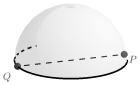
\includegraphics[width=\linewidth]{external/projective_1.pdf}
\end{sbspanel}%
\begin{sbspanel}{0.3}%
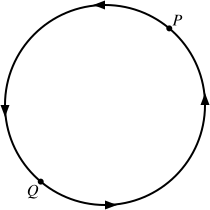
\includegraphics[width=\linewidth]{external/Projective_disk.pdf}
\end{sbspanel}%
\begin{sbspanel}{0.3}%
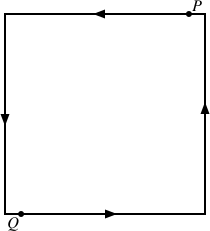
\includegraphics[width=\linewidth]{external/Projective_square.pdf}
\end{sbspanel}%
\end{sidebyside}%
\tcblower
\end{figureptx}%
By projecting the points on the hemisphere down to the \(xy\)-plane, we can represent \(S^2/\ssim\) as a disk whose antipodal points are identified, as seen in the middle in \hyperref[figure-F_projective_1]{Figure~{\xreffont\ref{figure-F_projective_1}}}. Use this last perspective to explain why \(\mathbb{R}P^2\) can be realized as a square where opposite sides are identified in opposite directions as shown at right in \hyperref[figure-F_projective_1]{Figure~{\xreffont\ref{figure-F_projective_1}}}.%
\item{}The projective plane \(\mathbb{R}P^2\) is a complicated object \textemdash{} it cannot be embedded in \(\R^3\) and so it is not something that can be easily visualized. The projective plane is a non-orientable surface and is also important in classifying surfaces \textemdash{} basically, every closed surface is made up of spheres, tori, and\slash{}or projective planes. In this part of the exercise we see how the projective plane itself is made by adjoining a Möbius strip to a disk (think of sewing the boundary of Möbius strip to the perimeter of a disk).%
\begin{enumerate}[font=\bfseries,label=(\roman*),ref=\theenumi.\roman*]%
\item{}Start with the model of \(\mathbb{R}P^2\) shown at left in \hyperref[figure-F_projective_2]{Figure~{\xreffont\ref{figure-F_projective_2}}}. Partition this object into three pieces as shown at right in \hyperref[figure-F_projective_2]{Figure~{\xreffont\ref{figure-F_projective_2}}}. Explain why the shaded region in the middle figure, separated out at right in \hyperref[figure-F_projective_2]{Figure~{\xreffont\ref{figure-F_projective_2}}}, is a Möbius strip.%
\begin{figureptx}{Figure}{Splitting the real projective plane.}{figure-F_projective_2}{}%
\begin{sidebyside}{3}{0}{0}{0}%
\begin{sbspanel}{0.333333333333333}[center]%
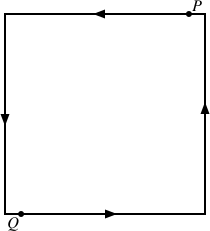
\includegraphics[width=\linewidth]{external/Projective_square.pdf}
\end{sbspanel}%
\begin{sbspanel}{0.333333333333333}[center]%
\includegraphics[width=\linewidth]{external/Projective_Mobius.pdf}
\end{sbspanel}%
\begin{sbspanel}{0.333333333333333}[center]%
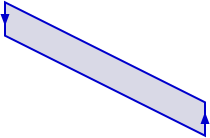
\includegraphics[width=\linewidth]{external/Projective_Mobius_split.pdf}
\end{sbspanel}%
\end{sidebyside}%
\tcblower
\end{figureptx}%
\item{}The space \(S\) that remains after we remove the Möbius strip from \(\mathbb{R}P^2\) is shown at left in \hyperref[figure-F_projective_3]{Figure~{\xreffont\ref{figure-F_projective_3}}}. The two spaces that follow are homeomorphic to \(S\). Describe the homeomorphisms that produce the spaces from \(S\). Then explain how \(\mathbf{R}P^2\) is obtained by attaching a Möbius strip to a disk along its boundary.%
\begin{figureptx}{Figure}{Recognizing the space \(S\).}{figure-F_projective_3}{}%
\begin{sidebyside}{5}{0}{0}{0}%
\begin{sbspanel}{0.2}[center]%
\includegraphics[width=\linewidth]{external/Projective_Disk_split.pdf}
\end{sbspanel}%
\begin{sbspanel}{0.2}[center]%
%
\begin{equation*}
\xrightarrow{f}
\end{equation*}
%
\end{sbspanel}%
\begin{sbspanel}{0.2}[center]%
\includegraphics[width=\linewidth]{external/Projective_Disk_hom_1.pdf}
\end{sbspanel}%
\begin{sbspanel}{0.2}[center]%
%
\begin{equation*}
\xrightarrow{g}
\end{equation*}
%
\end{sbspanel}%
\begin{sbspanel}{0.2}[center]%
\includegraphics[width=\linewidth]{external/Projective_Disk_hom_2.pdf}
\end{sbspanel}%
\end{sidebyside}%
\tcblower
\end{figureptx}%
\end{enumerate}%
\end{enumerate}%
\end{divisionexercise}%
\begin{divisionexercise}{11}{}{}{exercise-sec_quotients_exer-l}%
Let \(X = \R^2\) with the standard topology, and let \(Y = \{x \in \R \mid x \geq 0\}\) with the standard topology. Let \(f: X \to Y\) be defined by \(f((x,y)) = x^2+y^2\).%
\begin{enumerate}[font=\bfseries,label=(\alph*),ref=\alph*]%
\item{}Show that \(f\) is a continuous surjective function.%
\item{}Prove that the quotient space \(X^{*}\) of \(X\) defined by \(f\) is homeomorphic to \(Y\).%
\end{enumerate}%
\end{divisionexercise}%
\begin{divisionexercise}{12}{}{}{exercise-sec_quotients_exer-m}%
\index{retract}%
\index{retraction}%
Let \((X,\tau)\) be a topological space. A subspace \(A\) of \(X\) is a \terminology{retract} of \(X\) (or that \(X\) retracts onto \(A\)) if there is a continuous function \(r : X \to A\) such that \(r(a) = a\) for all \(a \in A\). Such a map \(r\) is called a \terminology{retraction}. Intuitively, a subspace \(A\) of \(X\) is a retract of \(X\) if we can continually collapse (or retract) \(X\) onto \(A\) without moving any of the points in \(A\). Certain types of retracts, namely deformation retracts, are important in algebraic topology.%
\begin{enumerate}[font=\bfseries,label=(\alph*),ref=\alph*]%
\item{}Show that every nonempty space can retract to a point.%
\item{}Show that \(\{-1,1\}\) is a retract of \(\R \setminus \{0\}\).%
\item{}Show that every retraction is a quotient map.%
\item{}Show that if \(X\) is Hausdorff and \(A\) is a retract of \(X\), then \(A\) must be a closed subset of \(X\).%
\end{enumerate}%
\end{divisionexercise}%
\begin{divisionexercise}{13}{}{}{exercise-sec_quotients_exer-n}%
For each of the following, answer true if the statement is always true. If the statement is only sometimes true or never true, answer false and provide a concrete example to illustrate that the statement is false. If a statement is true, explain why.%
\begin{enumerate}[font=\bfseries,label=(\alph*),ref=\alph*]%
\item{}Let \(p\) be a surjection from a topological space \(X\) to a nonempty set \(Y\). The quotient topology on \(Y\) is the largest topology on \(Y\) such that \(p\) is continuous.%
\item{}Let \(X = [0,1]\) with the Euclidean metric topology and define the relation \(\sim\) on \(X\) as \(x \sim y\) if \(x\) and \(y\) are either both rational or both irrational. Then the quotient space \(X/\ssim\) is a two point space with the indiscrete topology.%
\item{}Let \(p\) be a surjection from a topological space \(X\) to a nonempty set \(Y\). The quotient topology on \(Y\) is the largest topology on \(Y\) such that \(p\) is continuous.%
\item{}Let \(X = [0,1]\) with the Euclidean metric topology and define the relation \(\sim\) on \(X\) as \(x \sim y\) if \(x\) and \(y\) are either both rational or both irrational. Then the quotient space \(X/\ssim\) is a two point space with the indiscrete topology.%
\item{}If \(X\) is a topological space, \(Y\) is a set, and \(p: X \to Y\) is a surjection, then \(p(U)\) is open in the quotient topology whenever \(U\) is open in \(X\).%
\item{}If \(\sim\) is an equivalence relation on a topological space \(X\), then the quotient space \(X/\ssim\) is the set of all equivalence classes of \(X\) with the quotient topology.%
\end{enumerate}%
\end{divisionexercise}%
\end{exercises-section}
\end{chapterptx}
 %
%
\typeout{************************************************}
\typeout{Chapter 17 Compact Spaces}
\typeout{************************************************}
%
\begin{chapterptx}{Chapter}{Compact Spaces}{}{Compact Spaces}{}{}{chapter-chap_Compact_topology}
\renewcommand*{\chaptername}{Chapter}
\begin{objectives}{Focus Questions}{objectives-chap_Compact_topology-b}
%
\begin{itemize}[label=\textbullet]
\item{}What is a cover of a subset of a topological space? What is an open cover?%
\item{}What is a subcover of a cover?%
\item{}What is a compact subset of a topological space?%
\item{}What is one application of compactness?%
\item{}How do we characterize the compact subsets of \(\R^n\)? What theorem provides this characterization?%
\end{itemize}
\end{objectives}
%
%
\typeout{************************************************}
\typeout{Section  Introduction}
\typeout{************************************************}
%
\begin{sectionptx}{Section}{Introduction}{}{Introduction}{}{}{section-sec_compact_top_intro}
Closed and bounded intervals have important properties in calculus. Recall, for example, that every real-valued function that is continuous on a closed interval \([a, b]\) attains a maximum and minimum value on that interval. The question we want to address in this section is if there is a corresponding characterization for subsets of topological spaces that ensure that continuous real-valued functions with domains in topological spaces attain maximum and minimum values. The property that we will develop is called compactness.%
\par
The word ``compact'' might bring to mind a notion of smallness, but we need to be careful with the term. We might think that the interval \((0, 0.5)\) is small, but \((0, 0.5)\) is homeomorphic to \(\R\), which is not small. Similarly, we might think that the interval \([-10000, 10000]\) is large, but this interval is homeomorphic to the ``small'' interval \([-0.00001, 0.000001]\). As a result, the concept of compactness does not correspond to size, but rather structure, in a way. We will expand on this idea in this section.%
\par
Since a topology defines open sets, topological properties are often defined in terms of open sets. Let us consider an example to see if we can tease out some of the details we will need to get a useful notion of compactness. Consider the open interval \((0, 1)\) in \(\R\). Suppose we write \((0, 1)\) as a union of open balls. For example, let \(O_n = \left(\frac{1}{n}, 1-\frac{1}{n}\right)\) for \(n \in \Z^+\) and \(n \geq 3\). Notice that \((0, 1) \subseteq \bigcup_{n \geq 3} O_n\). Any collection of open sets whose union contains \((0, 1)\) is called an \terminology{open cover} of \((0, 1)\). Working with a larger number of sets is generally more complicated than working with a smaller number, so it is reasonable to ask if we can reduce the number of sets in our open cover of \((0, 1)\) and still cover \((0, 1)\). In particular, working with a finite collection of sets is preferable to working with an infinite number of sets (we can exhaustively check all of the possibilities in a finite setting if necessary). Notice that \(O_n \subset O_{n+1}\) for each \(n\), so we can eliminate many of the sets in this cover. However, if we eliminate enough sets so that we are left with only finitely many, then there will be a maximum value of \(n\) so that \(O_n\) remains in our collection. But then \(\frac{1}{2n}\) will not be in the union of our remaining collection of sets. As a result, we cannot find a finite collection of the \(O_n\) whose union contains \((0, 1)\). Note that there may be some collections of open sets that cover of \((0,1)\) for which there is a finite subcollection of sets that also cover \((0,1)\). For example, if we let \(U_n = \left(n-\frac{3}{4}, n+\frac{3}{4}\right)\), then \((0,1) \subseteq \bigcup_{n \in \Z} U_n\), and \((0,1) \subseteq U_{0} \cup U_1\). The main point is that there is at least one collection of open sets that covers \((0,1)\) for which there is no finite subcollection of sets that covers \((0,1)\).%
\par
Let's apply the same idea now to the set \([0, 1]\). Suppose we extend our open cover \(\{O_n\}\) to be an open cover of the closed interval \([0, 1]\) by including two additional open balls in \(\R\): \(O_0 = B(0, 0.5)\) and \(O_1 = B(1, 0.5)\). Now the sets \(O_0\), \(O_1\), and \(O_4\) form a finite collection of sets that covers \([0, 1]\). So even though the interval \([0, 1]\) is ``larger'' than \((0, 1)\) in the sense that \((0, 1) \subset [0, 1]\) we can represent \([0, 1]\) in a more efficient (that is finite) way in terms of open sets than we can the interval \((0, 1)\). This is the basic idea behind compactness.%
\begin{definition}{Definition}{}{definition-def_compact}%
\index{compact subset}%
A subset \(A\) of a topological space \(X\) is \terminology{compact} if for every set \(I\) and every family of open sets \(\{O_{\alpha}\}\) with \(\alpha \in I\) such that \(A \subseteq \bigcup_{\alpha \in I} O_{\alpha}\), there exists a finite subfamily \(\{O_{\alpha_1}, O_{\alpha_2}, \ldots, O_{\alpha_n}\}\) such that \(A \subseteq \bigcup_{i = 1}^n O_{\alpha_i}\).%
\end{definition}
If \((X,\tau)\) is a topological space and \(X\) is a compact subset of \(X\), then we say that \(X\) is a \terminology{compact topological space}. There is some terminology associated with \hyperref[definition-def_compact]{Definition~{\xreffont\ref{definition-def_compact}}}.%
\begin{definition}{Definition}{}{definition-sec_compact_top_intro-h}%
\index{cover}%
\index{cover!open}%
A \terminology{cover} of a subset \(A\) of a topological space \(X\) is a collection \(\{S_{\alpha}\}\) of subsets of \(X\) for \(\alpha\) in some indexing set \(I\) so that \(A \subseteq \bigcup_{\alpha \in I} S_{\alpha}\). In addition, if each set \(S_{\alpha}\) is an open set, then the collection \(\{S_{\alpha}\}\) is an \terminology{open cover} for \(A\).%
\end{definition}
\begin{definition}{Definition}{}{definition-sec_compact_top_intro-i}%
A \terminology{subcover} of a cover \(\{S_{\alpha}\}_{\alpha \in I}\) of a subset \(A\) of a topological space \(X\) is a collection \(\{S_{\beta}\}\) for \(\beta \in J\), where \(J\) is a subset of \(I\) such that \(A \subseteq \bigcup_{\beta \in J} S_{\beta}\). In addition, if \(J\) is a finite set, the subcover \(\{S_{\beta}\}_{\beta \in J}\) is a \terminology{finite subcover} of \(\{S_{\alpha}\}_{\alpha \in I}\).%
\end{definition}
So the sets \(O_0\), \(O_1\), and \(O_4\) in our previous example form a finite subcover of the open cover \(\{O_n\}_{n \geq 3}\).%
\par
Using the terminology we have now established, we can restate the definition of compactness in the following way: a subset \(A\) of a topological space \(X\) is compact if every open cover of \(A\) has a finite subcover of \(A\).%
\begin{exploration}{Preview Activity}{}{exploration-sec_compact_top_intro-l}%
Determine if the subset \(A\) of the topological space \(X\) is compact. Either prove \(A\) is compact by starting with an arbitrary infinite cover and demonstrating that there is a finite subcover, or find a specific infinite cover and prove that there is no finite subcover.%
\begin{enumerate}[font=\bfseries,label=(\alph*),ref=\alph*]%
\item{}\(A = \{-2, 3, e, \pi, 456875\}\) in \(X = \R\) with the Euclidean topology. Generalize this example.%
\item{}\(A = (0, 1]\) in \(X = \R\) with the Euclidean topology.%
\item{}\(A = \left\{\frac{1}{n} \mid n \in \Z^+\right\}\) in \(X = \R\) with the Euclidean topology.%
\item{}\(A = \Z^+\) in \(X = \R\) with the Euclidean topology.%
\item{}\(A = \Z^+\) in \(X = \R\) with the finite complement topology.%
\item{}\(A = \R\) in \(X = \R\) with the Euclidean topology.%
\end{enumerate}%
\end{exploration}%
There are two perspectives by which we can look at compactness. If \((X,\tau_X)\) is a topological space and \(A\) is a subset of \(X\), then \hyperref[definition-def_compact]{Definition~{\xreffont\ref{definition-def_compact}}} tells us what it means for \(A\) to be compact as a subset of \(X\). From this perspective, we use open sets in \(X\) to make open covers of \(A\). We can also consider \(A\) as a subspace of \(X\) using the subspace topology \(\tau_A\). From this perspective we can examine the compactness of \(A\) using relatively open sets for open covers. \hyperlink{exercise-ex_subspace_compact}{Exercise~{\xreffont 14}} tells us that these two perspectives are equivalent, so we will use whatever perspective is appropriate for a given situation.%
\end{sectionptx}
%
%
\typeout{************************************************}
\typeout{Section  Compactness and Continuity}
\typeout{************************************************}
%
\begin{sectionptx}{Section}{Compactness and Continuity}{}{Compactness and Continuity}{}{}{section-sec_compact_cont}
In our preview activity we learned about compactness \textemdash{} the analog of closed intervals from \(\R\) in topological spaces. Recall that a subset \(A\) of a topological space \(X\) is compact if every open cover of \(A\) has a finite sub-cover. As we will see, the definition of compactness is exactly what we need to ensure results of the type that continuous real-valued functions with domains in topological spaces attain maximum and minimum values on compact sets.%
\par
We might expect that compact sets have certain properties, but we must be careful which ones we assume.%
\begin{activity}{Activity}{}{activity-act_compact_clopen}%
Let \(X = \{a,b,c,d\}\) and give \(X\) the topology \(\tau = \{\emptyset, \{a\}, \{b,c\}, \{a,b,c\}, X\}\).%
\begin{enumerate}[font=\bfseries,label=(\alph*),ref=\alph*]%
\item{}Explain why every finite subset of a topological space must be compact.%
\item{}Find, if possible, a subset of \(X\) that is compact and open. If no such subset exists, explain why.%
\item{}If \(A\) is a compact subset of \(X\), must \(A\) be open? Explain.%
\item{}Find, if possible, a subset of \(X\) that is compact and closed. If no such subset exists, explain why.%
\item{}If \(A\) is a compact subset of \(X\), must \(A\) be closed? Explain.%
\end{enumerate}%
\end{activity}%
The message of \hyperref[activity-act_compact_clopen]{Activity~{\xreffont\ref{activity-act_compact_clopen}}} is that compactness by itself is not related to closed or open sets. We will see later, though, that in some reasonable circumstances, compact sets and closed sets are related. For the moment, we take a short detour and ask if compactness is a topological property.%
\begin{activity}{Activity}{}{activity-act_compact_invariant}%
Let \((X, \tau_X)\) and \((Y, \tau_Y)\) be topological spaces, and let \(f: X \to Y\) be continuous. Assume that \(A\) is a compact subset of \(X\). In this activity we want to determine if \(f(A)\) must be a compact subset of \(Y\).%
\begin{enumerate}[font=\bfseries,label=(\alph*),ref=\alph*]%
\item{}What do we need to show to prove that \(f(A)\) is a compact subset of \(Y\)? Where do we start?%
\item{}If we have an open cover of \(f(A)\) in \(Y\), how can we find an open cover \(\{U_{\alpha}\}\) for \(A\)? Be sure to verify that what you claim is actually an open cover of \(A\).%
\item{}What do we know about any open cover of \(A\)?%
\item{}Complete the proof of the following theorem.%
\begin{theorem}{Theorem}{}{}{theorem-act_compact_invariant-e-a-b}%
Let \((X, \tau_X)\) and \((Y, \tau_Y)\) be topological spaces, and let \(f: X \to Y\) be continuous. If \(A\) is a compact subset of \(X\), then \(f(A)\) is a compact subset of \(Y\).%
\end{theorem}
\end{enumerate}%
\end{activity}%
A consequence of \hyperref[activity-act_compact_invariant]{Activity~{\xreffont\ref{activity-act_compact_invariant}}} is that compactness is a topological property.%
\begin{corollary}{Corollary}{}{}{corollary-sec_compact_cont-h}%
Let \((X, \tau_X)\) and \((Y, \tau_Y)\) be homeomorphic topological spaces. Then a subset \(A\) of \(X\) is compact if and only if \(f(A)\) is compact in \(Y\).%
\end{corollary}
\end{sectionptx}
%
%
\typeout{************************************************}
\typeout{Section  Compact Subsets of \(\R^n\)}
\typeout{************************************************}
%
\begin{sectionptx}{Section}{Compact Subsets of \(\R^n\)}{}{Compact Subsets of \(\R^n\)}{}{}{section-sec_compact_rn}
The metric space \((\R^n,d_E)\) is not compact since the open cover \(\{B(0, n)\}_{n \in \Z^+}\) has no finite sub-cover. Since we have already shown that \((\R,d_E)\) is homeomorphic to the topological subspaces \((a,b)\), \((-\infty, b)\), and \((a,\infty)\) for any \(a,
b \in \R\), we conclude that no open intervals are compact. Similarly, no half-closed intervals are compact. In fact, we will demonstrate in this section that the compact subsets of \((\R^n, d_E)\) are exactly the subsets that are closed and bounded. The first step is contained in the next activity.%
\begin{activity}{Activity}{}{activity-act_metric_compact_closed}%
We have seen that compact sets can be either open or closed. However, in certain situations compact sets must be closed. We investigate that idea in this activity. Let \(A\) be a compact subset of a Hausdorff topological space \(X\). We will examine why \(A\) must be a closed set.%
\begin{enumerate}[font=\bfseries,label=(\alph*),ref=\alph*]%
\item{}To prove that \(A\) is a closed set, we consider the set \(X \setminus A\). What property of \(X \setminus A\) will ensure that \(A\) is closed? How do we prove that \(X \setminus A\) has this property?%
\item{}Let \(x \in X \setminus A\). Assume that \(A\) is a nonempty set (why can we make this assumption)? For each \(a \in A\), why must there exist disjoint open sets \(O_{xa}\) and \(O_a\) with \(x \in O_{xa}\) and \(a \in O_a\)?%
\item{}Why must there exist a positive integer \(n\) and elements \(a_1\), \(a_2\), \(\ldots\), \(a_n\) in \(A\) such that the sets \(O_{a_1}\), \(O_{a_2}\), \(\ldots\), \(O_{a_n}\) form an open cover of \(A\)?%
\item{}Now find an open subset of \(X \setminus A\) that has \(x\) as an element. What does this tell us about \(A\)?%
\end{enumerate}%
\end{activity}%
The result of \hyperref[activity-act_metric_compact_closed]{Activity~{\xreffont\ref{activity-act_metric_compact_closed}}} is summarized in \hyperref[theorem-thm_metric_compact_closed]{Theorem~{\xreffont\ref{theorem-thm_metric_compact_closed}}}.%
\begin{theorem}{Theorem}{}{}{theorem-thm_metric_compact_closed}%
If \(A\) is a compact subset of a Hausdorff topological space, then \(A\) is closed.%
\end{theorem}
\hyperref[theorem-thm_metric_compact_closed]{Theorem~{\xreffont\ref{theorem-thm_metric_compact_closed}}} tells us something about compact subsets of \((\R^n, d_E)\). Since every metric space is Hausdorff, we can conclude the following corollary.%
\begin{corollary}{Corollary}{}{}{corollary-sec_compact_rn-g}%
If \(A\) is a compact subset of \((\R^n, d_E)\), then \(A\) is closed.%
\end{corollary}
To classify the compact subsets of \((\R^n, d_E)\) as closed and bounded, we need to discuss what it means for a set in \(\R^n\) to be bounded. The basic idea is straightforward \textemdash{} a subset of \(\R^n\) is bounded if it doesn't go off to infinity in any direction. In other words, a subset \(A\) of \(\R^n\) is bounded if we can construct a box in \(\R^n\) that is large enough to contain it. Thus, the following definition.%
\begin{definition}{Definition}{}{definition-def_n_cube}%
\index{bounded subset of \(\R^n\)}%
A subset \(A\) of \(\R^n\) is \terminology{bounded} if there exists \(M \gt 0\) such that \(A \subseteq Q^n_M\), where%
\begin{equation*}
Q^n_M = \{(x_1,x_2, \ldots, x_n) \mid -M \leq x_i \leq M \text{ for every }  1 \leq i \leq n\}\text{.}
\end{equation*}
%
\end{definition}
The set \(Q^n_M\) in \hyperref[definition-def_n_cube]{Definition~{\xreffont\ref{definition-def_n_cube}}} is called the \terminology{standard} \(n\)\terminology{-dimensional cube of size M}. A standard 3-dimensional cube of size \(M\) is shown in \hyperref[figure-F_M_cube]{Figure~{\xreffont\ref{figure-F_M_cube}}}.%
\begin{figureptx}{Figure}{A standard 3-cube \(Q^3_M\).}{figure-F_M_cube}{}%
\begin{image}{0.3}{0.4}{0.3}{}%
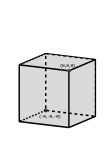
\includegraphics[width=\linewidth]{external/M_cube.pdf}
\end{image}%
\tcblower
\end{figureptx}%
An important fact about standard \(n\)-cubes is that they are compact subsets of \(\R^n\). Compactness is a complicated property \textemdash{} it is difficult to prove a result that is true about every open cover. As a result, the proof of \hyperref[theorem-thm_Compact_cubes]{Theorem~{\xreffont\ref{theorem-thm_Compact_cubes}}} is quite technical, but it is a critical step to classifying the compact subsets of \(\R^n\).%
\begin{theorem}{Theorem}{}{}{theorem-thm_Compact_cubes}%
Let \(n \in \Z^+\). The standard \(n\)-dimensional cube of size \(M\) is a compact subset of \(\R^n\) for any \(M \gt 0\).%
\end{theorem}
\begin{proof}{Proof}{}{proof-thm_Compact_cubes-b}
We proceed by contradiction and assume that there is an \(n \in \Z^+\) and a positive real number \(M\) such that \(Q^n_M\) is not compact. So there exists an open cover \(\{O_{\alpha}\}\) with \(\alpha\) in some indexing set \(I\) of \(Q^n_M\) that has no finite sub-cover. Let \(Q_0 = Q^n_M\) so that \(Q_0\) is an \(n\)-cube with side length \(2M\). Partition \(Q_0\) into \(2^n\) uniform sub-cubes of side length \(M = \frac{2M}{2}\) (a picture for \(n=2\) is shown at left in \hyperref[figure-F_Cubes]{Figure~{\xreffont\ref{figure-F_Cubes}}}).%
\begin{figureptx}{Figure}{Left : \(Q_1\). Middle: \(Q_2\). Right: Labeling the corners.}{figure-F_Cubes}{}%
\begin{sidebyside}{3}{0}{0}{0}%
\begin{sbspanel}{0.333333333333333}%
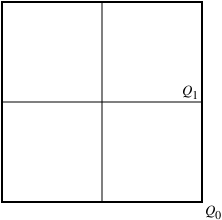
\includegraphics[width=\linewidth]{external/HB_cube.pdf}
\end{sbspanel}%
\begin{sbspanel}{0.333333333333333}%
\includegraphics[width=\linewidth]{external/HB_cube_2.pdf}
\end{sbspanel}%
\begin{sbspanel}{0.333333333333333}%
\includegraphics[width=\linewidth]{external/HB_cube_3.pdf}
\end{sbspanel}%
\end{sidebyside}%
\tcblower
\end{figureptx}%
Let \(Q'_0\) be one of these sub-cubes. The collection \(\{O_{\alpha} \cap Q'_0\}_{\alpha \in I}\) is an open cover of \(Q'_0\) in the subspace topology. If each of these open covers has a finite sub-cover, then we can take the union of all of the \(O_{\alpha}\)s over all of the finite sub-covers to obtain a finite sub-cover of \(\{O_{\alpha}\}_{\alpha \in I}\) for \(Q_0\). Since our cover \(\{O_{\alpha}\}_{\alpha \in I}\) for \(Q_0\) has no finite sub-cover, we conclude that there is one sub-cube, \(Q_1\), for which the open cover \(\{O_{\alpha} \cap Q_1\}_{\alpha \in I}\) has no finite sub-cover. Now we repeat the process and partition \(Q_1\) into \(2^n\) uniform sub-cubes of side length \(\frac{M}{2}= \frac{2M}{2^2}\). The same argument we just made tells us that there is a sub-cube \(Q_2\) of \(Q_1\) for which the open cover \(\{O_{\alpha} \cap Q_2\}_{\alpha \in I}\) has no finite sub-cover (an illustration for the \(n=2\) case is shown at middle in \hyperref[figure-F_Cubes]{Figure~{\xreffont\ref{figure-F_Cubes}}}). We proceed inductively to obtain an infinite nested sequence%
\begin{equation*}
Q_0 \supset Q_1 \supset Q_2 \supset Q_3 \supset \cdots \supset Q_k \supset \cdots
\end{equation*}
of cubes such that for each \(k \in \Z\), the lengths of the sides of cube \(Q_k\) are \(\frac{M}{2^{k-1}} = \frac{2M}{2^{k}}\) and the open cover \(\{O_{\alpha} \cap Q_k\}_{\alpha \in I}\) of \(Q_k\) has no finite sub-cover. Now we show that \(\bigcap_{k=1}^{\infty} Q_k \neq \emptyset\).%
\par
For \(i \in \Z^+\), let \(Q_i = [a_{i,1}, b_{i,1}] \times [a_{i,2}, b_{i,2}] \times \cdots [a_{i,n}, b_{i,n}]\). That is, think of the point \((a_{i,1}, a_{i,2}, \ldots,
a_{i,n})\) as a lower corner of the cube and the point \((b_{i,1}, b_{i,2}, \ldots,
b_{i,n})\) as an upper corner of the \(n\)-cube \(Q_i\) (a labeling for \(n=2\) and \(i\) from 1 to 3 is shown at right in \hyperref[figure-F_Cubes]{Figure~{\xreffont\ref{figure-F_Cubes}}}). Let \(q = (\sup\{a_{i,1}\}, \sup\{a_{i,2}\}, \ldots, \sup\{a_{i,n}\})\). We will show that \(q \in \bigcap_{k=1}^{\infty} Q_k\). Fix \(r \in \Z^+\). We need to demonstrate that%
\begin{equation*}
q \in Q_r = \{(x_1, x_2, \ldots, x_n) \mid a_{r,s} \leq x_s \leq b_{r,s} \text{ for each }  1 \leq s \leq n\}\text{.}
\end{equation*}
%
\par
For each \(s\) between 1 and \(n\) we have%
\begin{equation}
a_{r,s} \leq \sup\{a_{i,s}\}\label{men-eq_cube_a}
\end{equation}
because \(\sup\{a_{i,s}\}\) is an upper bound for all of the \(a_{i,s}\). The fact that our cubes are nested means that%
\begin{align}
a_{1,s} \amp \leq a_{2,s} \leq \cdots,\notag\\
b_{1,s} \amp \geq b_{2,s} \geq \cdots,\notag\\
a_{i,s} \amp \leq b_{i,s}\label{mrow-eq_cube_b}
\end{align}
for every \(i\) and \(s\). Since \(\sup\{a_{i,s}\}\) is the least upper bound of all of the \(a_{i,s}\), property \hyperref[mrow-eq_cube_b]{({\xreffont\ref{mrow-eq_cube_b}})} shows that \(\sup\{a_{i,s}\} \leq b_{i,s}\) for every \(i\). Thus, \(\sup\{a_{i,s}\} \leq b_{r,s}\) and so \(a_{r,s} \leq \sup\{a_{i,s}\} \leq b_{r,s}\). This shows that \(q \in Q_k\) for every \(k\). Consequently, \(q \in \bigcap_{k=1}^{\infty} Q_k\) and \(\bigcap_{k=1}^{\infty} Q_k\) is not empty. (The fact that the side lengths of our cubes are converging to 0 implies that \(\bigcap_{k=1}^{\infty} Q_k = \{q\}\), but we only need to know that \(\bigcap_{k=1}^{\infty} Q_k\) is not empty for our proof.)%
\par
Since \(\{O_{\alpha}\}_{\alpha \in I}\) is a cover for \(Q_0\), there must exist an \(\alpha_q \in I\) such that \(q \in O_{\alpha_q}\). The set \(O_{\alpha_q}\) is open, so there exists \(\epsilon_q \gt 0\) such that \(B(q, \epsilon_q) \subseteq O_{\alpha_q}\). The maximum distance between points in \(Q_k\) is the distance between the corner points \((a_{k,1}, a_{k,2}, \ldots,
a_{k,n})\) and \((b_{k,1}, b_{k,2}, \ldots, b_{k,n})\), where each length \(b_{k,s} - a_{k,s}\) is \(\frac{M}{2^{k-1}}\). The distance formula tells us that this maximum distance between points in \(Q_k\) is%
\begin{equation*}
D_k = \sqrt{ \sum_{s=1}^n \left(\frac{M}{2^{k-1}}\right)^2} =  \sqrt{ n \left(\frac{M}{2^{k-1}}\right)^2} = \frac{M}{2^{k-1}} \sqrt{n}\text{.}
\end{equation*}
%
\par
Now choose \(K \in \Z^+\) such that \(D_K \lt \epsilon_q\). Then if \(x \in Q_K\) we have \(d_E(q,x)\lt D_K\) and \(x \in B(q, \epsilon_q)\). So \(Q_K \subseteq B(q, \epsilon_q)\). But \(B(q, \epsilon_q) \subseteq O_{\alpha_q}\). So the collection \(\{O_{\alpha_q} \cap Q_K\}\) is a sub-cover of \(\{O_{\alpha} \cap Q_K\}_{\alpha \in I}\) for \(Q_K\). But this contradicts the fact this open cover has no finite sub-cover. The assumption that led us to this contradiction was that \(Q_0\) was not compact, so we conclude that the standard \(n\)-dimensional cube of size \(M\) is a compact subset of \(\R^n\) for any \(M \gt 0\).%
\end{proof}
One consequence of \hyperref[theorem-thm_Compact_cubes]{Theorem~{\xreffont\ref{theorem-thm_Compact_cubes}}} is that any closed interval \([a,b]\) in \(\R\) is a compact set. But we can say even more \textemdash{} that the compact subsets of \(\R^n\) are the closed and bounded subsets. This will require one more intermediate result about closed subsets of compact topological spaces.%
\begin{activity}{Activity}{}{activity-sec_compact_rn-o}%
Let \(X\) be a compact topological space and \(C\) a closed subset of \(X\). In this activity we will prove that \(C\) is compact.%
\begin{enumerate}[font=\bfseries,label=(\alph*),ref=\alph*]%
\item{}What does it take to prove that \(C\) is compact?%
\item{}Use an open cover for \(C\) and the fact that \(C\) is closed to make an open cover for \(X\).%
\item{}Use the fact that \(X\) is compact to complete the proof of the following theorem.%
\begin{theorem}{Theorem}{}{}{theorem-thm_closed_compact}%
Let \(X\) be a compact topological space. Then any closed subset of \(X\) is compact.%
\end{theorem}
\end{enumerate}%
\end{activity}%
Now we can prove a major result, that the compact subsets of \((\R^n, d_E)\) are the closed and bounded subsets. This result is important enough that it is given a name.%
\begin{theorem}{Theorem}{The Heine-Borel Theorem.}{}{theorem-sec_compact_rn-q}%
A subset \(A\) of \((\R^n, d_E)\) is compact if and only if \(A\) is closed and bounded.%
\end{theorem}
\begin{proof}{Proof}{}{proof-sec_compact_rn-q-c}
Let \(A\) be a subset of \((\R^n, d_E)\). Assume that \(A\) is closed and bounded. Since \(A\) is bounded, there is a positive number \(M\) such that \(A \subseteq Q^n_M\). \hyperref[theorem-thm_Compact_cubes]{Theorem~{\xreffont\ref{theorem-thm_Compact_cubes}}} shows that \(Q^n_M\) is compact, and then \hyperref[theorem-thm_closed_compact]{Theorem~{\xreffont\ref{theorem-thm_closed_compact}}} shows that \(A\) is compact.%
\par
For the converse, assume that \(A\) is a compact subset of \(\R^n\). We must show that \(A\) is closed and bounded. Now \((\R^n, d_E)\) is a metric space, and so Hausdorff. \hyperref[theorem-thm_metric_compact_closed]{Theorem~{\xreffont\ref{theorem-thm_metric_compact_closed}}} then shows that \(A\) is closed. To conclude our proof, we need to demonstrate that \(A\) is bounded. For each \(k \gt 0\), let%
\begin{equation*}
O_k = \{ (x_1,x_2, \ldots, x_n) \mid -k \lt  x_i \lt  k \text{ for every }  1 \leq i \leq n\}\text{.}
\end{equation*}
%
\par
That is, \(O_k\) is the open \(k\)-cube in \(\R^n\). Next let%
\begin{equation*}
U_k = O_k \cap A
\end{equation*}
for each \(k\). Since \(\bigcup_{k \gt 0} O_k = \R^n\), it follows that \(\{U_k\}_{k \gt 0}\) is an open cover of \(A\). The fact that \(A\) is compact means that there is a finite collection \(U_{k_1}\), \(U_{k_2}\), \(\ldots\), \(U_{k_m}\) of sets in \(\{U_k\}_{k \gt 0}\) that cover \(A\). Let \(K = \max\{k_i \mid 1 \leq i \leq m\}\). Then \(U_{k_i} \subseteq U_K\) for each \(i\), and so \(A \subseteq U_K \subset Q^m_K\). Thus, \(A\) is bounded. This completes the proof that if \(A\) is compact in \(\R^n\), then \(A\) is closed and bounded.%
\end{proof}
You might wonder whether the Heine-Borel Theorem is true in any metric space.%
\begin{activity}{Activity}{}{activity-sec_compact_rn-s}%
A subset \(A\) of a metric space \((X, d)\) is bounded if there exists a real number \(M\) such that \(d(a_1,a_2) \leq M\) for all \(a_1, a_2 \in A\). (This is equivalent to our definition of a bounded subset of \(\R^n\) given earlier, but works in any metric space.) Explain why \(\Z\) as a subset of \((\R,d)\), where \(d\) is the discrete metric, is closed and bounded but not compact.%
\end{activity}%
\end{sectionptx}
%
%
\typeout{************************************************}
\typeout{Section  An Application of Compactness}
\typeout{************************************************}
%
\begin{sectionptx}{Section}{An Application of Compactness}{}{An Application of Compactness}{}{}{section-sec_compact_app}
As mentioned at the beginning of this section, compactness is the quality we need to ensure that continuous functions from topological spaces to \(\R\) attain their maximum and minimum values.%
\begin{activity}{Activity}{}{activity-sec_compact_app-c}%
In this activity we prove the following theorem.%
\begin{theorem}{Theorem}{}{}{theorem-thm_max_min}%
A continuous function from a compact topological space to the real numbers assumes a maximum and minimum value.%
\end{theorem}
\begin{enumerate}[font=\bfseries,label=(\alph*),ref=\alph*]%
\item{}Let \(X\) be a compact topological space and \(f: X \to \R\) a continuous function. What does the continuity of \(f\) tell us about \(f(X)\) in \(\R\)?%
\item{}Why can we conclude that the set \(f(X)\) has a least upper bound \(M\)? Why must \(M\) be an element of \(f(X)\)?%
\item{}Complete the proof of \hyperref[theorem-thm_max_min]{Theorem~{\xreffont\ref{theorem-thm_max_min}}}.%
\end{enumerate}%
\end{activity}%
\end{sectionptx}
%
%
\typeout{************************************************}
\typeout{Section  Summary}
\typeout{************************************************}
%
\begin{sectionptx}{Section}{Summary}{}{Summary}{}{}{section-sec_compact_top_summ}
Important ideas that we discussed in this section include the following.%
\begin{itemize}[label=\textbullet]
\item{}A cover of a subset \(A\) of a topological space \(X\) is any collection of subsets of \(X\) whose union contains \(A\). An open cover is a cover consisting of open sets.%
\item{}A subcover of a cover of a set \(A\) is a subset of the cover such that the union of the sets in the subcover also contains \(A\).%
\item{}A subset \(A\) of a topological space is compact if every open cover of \(A\) has a finite subcover.%
\item{}A continuous function from a compact topological space to the real numbers must attain a maximum and minimum value.%
\item{}The Heine-Borel Theorem states that the compact subsets of \(\R^n\) are exactly the subsets that are closed and bounded.%
\end{itemize}
%
\end{sectionptx}
%
%
\typeout{************************************************}
\typeout{Exercises  Exercises}
\typeout{************************************************}
%
\begin{exercises-section}{Exercises}{Exercises}{}{Exercises}{}{}{exercises-sec_compact_top_exer}
\begin{divisionexercise}{1}{}{}{exercise-sec_compact_top_exer-b}%
\begin{enumerate}[font=\bfseries,label=(\alph*),ref=\alph*]%
\item{}Determine the compact subsets of a topological space \(X\) with the indiscrete topology.%
\item{}Determine the compact subsets of a topological space \(X\) with the indiscrete topology.%
\end{enumerate}%
\end{divisionexercise}%
\begin{divisionexercise}{2}{}{}{exercise-sec_compact_top_exer-c}%
Recall from \hyperref[definition-def_weaker_topologies]{Definition~{\xreffont\ref{definition-def_weaker_topologies}}} that if \(\tau_1\) and \(\tau_2\) are two topologies on a set \(X\) such that \(\tau_1 \subseteq \tau_2\), then \(\tau_1\) is said to be a \terminology{coarser} (or \terminology{weaker}) topology than \(\tau_2\), or \(\tau_2\) is a \terminology{finer} (or \terminology{stronger}) topology than \(\tau_1\). In this exercise we explore the question of whether compactness is a property that is passed from weaker to stronger topologies or from stronger to weaker. Let \(\tau_1\) and \(\tau_2\) be two topologies on a set \(X\). If \(\tau_1 \subseteq \tau_2\), what does compactness under \(\tau_1\) or \(\tau_2\) imply, if anything, about compactness under the other topology? Justify your answers.%
\end{divisionexercise}%
\begin{divisionexercise}{3}{}{}{exercise-ex_intersection_not_compact}%
Let \(\E\) be the set of even integers, and let \(\tau = \{\Z\} \cup \{O \subseteq \E\}\). That is, \(\tau\) is the collection of all subsets of \(\E\) along with \(\Z\).%
\begin{enumerate}[font=\bfseries,label=(\alph*),ref=\alph*]%
\item{}Prove that \(\tau\) is a topology on \(\Z\).%
\item{}Find all compact subsets of \((\Z, \tau)\). Verify your answer.%
\item{}Prove or disprove: If \(A\) and \(B\) are compact subsets of a topological space \(X\), then \(A \cap B\) is also a compact subset of \(X\).%
\end{enumerate}%
\end{divisionexercise}%
\begin{divisionexercise}{4}{}{}{exercise-sec_compact_top_exer-e}%
Let \((X,\tau)\) be a topological space%
\begin{enumerate}[font=\bfseries,label=(\alph*),ref=\alph*]%
\item{}Prove that the union of any finite number of compact subsets of \(X\) is a compact subset of \(X\).%
\item{}In \hyperlink{exercise-ex_intersection_not_compact}{Exercise~{\xreffont 3}} we should have seen that the intersection of compact sets is not necessarily compact. If \(X\) is Hausdorff, prove that the intersection of any finite number of compact subsets of \(X\) is a compact subset of \(X\).%
\end{enumerate}%
\end{divisionexercise}%
\begin{divisionexercise}{5}{}{}{exercise-sec_compact_top_exer-f}%
Consider \(\Z\) with the digital line topology (see \hyperlink{exercise-ex_digital_line_topology}{Exercise~{\xreffont 11}}). Determine the compact subsets of \(\Z\).%
\end{divisionexercise}%
\begin{divisionexercise}{6}{}{}{exercise-sec_compact_top_exer-g}%
For each \(n \in \Z^+\), let \((-n,n)\) be the set of integers in the interval \((-n,n)\) (see \hyperlink{exercise-ex_coarse_topology_example}{Exercise~{\xreffont 4}}.)%
\begin{enumerate}[font=\bfseries,label=(\alph*),ref=\alph*]%
\item{}Show that \(\B = \{(-n,n)\}_{n \in \Z^+}\) is a basis for a topology \(\tau\) on \(\Z\)%
\item{}Is the subset \((-2,2)\) compact in this topology?%
\item{}Determine all of the compact subsets of \(\Z\).%
\end{enumerate}%
\end{divisionexercise}%
\begin{divisionexercise}{7}{}{}{exercise-sec_compact_top_exer-h}%
Let \(X\) and \(Y\) be topological spaces, and let \(f: X \to Y\) be a function.%
\begin{enumerate}[font=\bfseries,label=(\alph*),ref=\alph*]%
\item{}Suppose that \(f\) is a continuous function, and that \(X\) is compact and \(Y\) is Hausdorff. Prove that if \(C\) is a closed subset of \(X\), then \(f(C)\) is a closed subset of \(Y\). (Thus, \(f\) is a \terminology{closed} function.)%
\par\smallskip%
\noindent\textbf{\blocktitlefont Hint}.\hypertarget{hint-sec_compact_top_exer-h-b-b}{}\quad{}Use Activity 17.3, Activity 17.4, and Theorem 17.6.%
\item{}Suppose that \(f\) is a continuous bijection. Prove that if \(X\) is compact and \(Y\) is Hausdorff, then \(f\) is a homeomorphism.%
\item{}Give an example where \(f\) is a continuous bijection and \(X\) is compact, but \(f\) is not a homeomorphism.%
\item{}Give an example where \(f\) is a continuous bijection and \(Y\) is Hausdorff, but \(f\) is not a homeomorphism.%
\end{enumerate}%
\end{divisionexercise}%
\begin{divisionexercise}{8}{}{}{exercise-sec_compact_top_exer-i}%
The Either-Or topology on the interval \(X = [-1,1]\) has as its open sets all subsets of \(X\) that contain \((-1,1)\) and any subset of \(X\) that doesn't contain \(0\).%
\begin{enumerate}[font=\bfseries,label=(\alph*),ref=\alph*]%
\item{}Describe the non-trivial closed subsets of \(X\).%
\item{}Is \(X\) a Hausdorff topological space? Explain.%
\item{}Is \(X\) compact? Prove your answer.%
\item{}Are there any subsets of \(\Z\) that are not compact? Justify your answer.%
\end{enumerate}%
\end{divisionexercise}%
\begin{divisionexercise}{9}{}{}{exercise-ex_K_topology_compact}%
Let \(K = \left\{\frac{1}{k} \mid k \text{ is a positive integer} \right\}\). Let \(\B\) be the collection of all open intervals of the form \((a,b)\) and all sets of the form \((a,b) \setminus K\), where \(a \lt b\) are real numbers as in \hyperref[example-exp_K_topology]{Example~{\xreffont\ref{example-exp_K_topology}}}. Let \(\tau_K\) be the topology generated by \(\B\).%
\begin{enumerate}[font=\bfseries,label=(\alph*),ref=\alph*]%
\item{}Show that \((\R, \tau_K)\) is not compact.%
\par\smallskip%
\noindent\textbf{\blocktitlefont Hint}.\hypertarget{hint-ex_K_topology_compact-b-b}{}\quad{}How is the \(K\)-topology related to the Euclidean topology?%
\item{}Show that any subset of \(\R\) that contains \(K\) is not a compact subset of \((\R, \tau_K)\). In particular, even though \([0,1]\) is a closed and bounded subset of \(\R\) in \((\R, \tau_K)\), we note that \([0,1]\) is not compact.%
\par\smallskip%
\noindent\textbf{\blocktitlefont Hint}.\hypertarget{hint-ex_K_topology_compact-c-b}{}\quad{}Consider the sets \(O_k = \left(\frac{1}{k},2\right) \cup (-1,1) \setminus K\) for \(k \in \Z^+\).%
\end{enumerate}%
\end{divisionexercise}%
\begin{divisionexercise}{10}{}{}{exercise-ex_Compact_normal}%
Let \(X\) be a topological space.%
\begin{enumerate}[font=\bfseries,label=(\alph*),ref=\alph*]%
\item{}Prove that if \(X\) is Hausdorff and \(C\) is a compact subset of \(X\), then for each \(x \in X \setminus C\) there exist disjoint open sets \(U\) and \(V\) such that \(x \in U\) and \(C \subseteq V\).%
\item{}Prove that if \(X\) is a compact Hausdorff space, then \(X\) is normal.%
\end{enumerate}%
\end{divisionexercise}%
\begin{divisionexercise}{11}{}{}{exercise-sec_compact_top_exer-l}%
Let \(X\) be a nonempty set and let \(p\) be a fixed element in \(X\). Let \(\tau_p\) be the particular point topology and \(\tau_{\overline{p}}\) the excluded point topology on \(X\). That is%
\begin{itemize}[label=\textbullet]
\item{}\(\tau_{p}\) is the collection of subsets of \(X\) consisting of \(\emptyset\), \(X\), and all of the subsets of \(X\) that contain \(p\).%
\item{}\(\tau_{\overline{p}}\) is the collection of subsets of \(X\) consisting of \(\emptyset\), \(X\), and all of the subsets of \(X\) that do not contain \(p\).%
\end{itemize}
That the particular point and excluded point topologies are topologies is the subject of \hyperlink{exercise-ex_particular_point_topology}{Exercise~{\xreffont 9}} and \hyperlink{exercise-ex_excluded_point_topology}{Exercise~{\xreffont 10}}. Determine, with proof, the compact subsets of \(X\) when%
\begin{enumerate}[font=\bfseries,label=(\alph*),ref=\alph*]%
\item{}\(X\) has the particular point topology \(\tau_p\)%
\item{}\(X\) has the excluded point topology \(\tau_{\overline{p}}\).%
\end{enumerate}%
\end{divisionexercise}%
\begin{divisionexercise}{12}{}{}{exercise-sec_compact_top_exer-m}%
In this exercise we encounter a non-Hausdorff topological space in which single points sets are closed, and in which compact subsets need not be closed. Consider the set \(\Z\) with the finite complement topology \(\tau_{FC}\).%
\begin{enumerate}[font=\bfseries,label=(\alph*),ref=\alph*]%
\item{}Show that every single point set is closed.%
\item{}Explain why \((\Z, \tau_{FC})\) is not a Hausdorff space.%
\item{}Let \(U\) be an open set in \((\Z, \tau_{FC})\) that contains \(0\) and \(V\) an open set in \((\Z, \tau_{FC})\) that contains \(1\). Explain why it cannot be the case that \(U\) and \(V\) are disjoint \textemdash{} that is, \(U \cap V\) must be non-empty.%
\item{}Show that the subset \(\E\) of even integers is a compact subset of \((\Z, \tau_{FC})\) that is not closed. Verify your result.%
\end{enumerate}%
\end{divisionexercise}%
\begin{divisionexercise}{13}{}{}{exercise-sec_compact_top_exer-n}%
Let \((X, \tau)\) be a Hausdorff topological space.%
\begin{enumerate}[font=\bfseries,label=(\alph*),ref=\alph*]%
\item{}Let \(x \in X\) and let \(A\) be a compact subset of \(X\). Prove that there exist disjoint open subsets \(U\) and \(V\) of \(X\) such that \(x \in U\) and \(A \subseteq V\).%
\item{}Let \(A\) and \(B\) be disjoint compact subsets of \(X\). Prove that there exist disjoint open sets \(U\) and \(V\) such that \(A \subseteq U\) and \(B \subseteq V\).%
\end{enumerate}%
\end{divisionexercise}%
\begin{divisionexercise}{14}{}{}{exercise-ex_subspace_compact}%
Let \((X,\tau_X)\) be a topological space and let \(A\) be a subset of \(X\). Let \(\tau_A\) be the subspace topology on \(A\). Prove that \(A\) is a compact subset of \(X\) if and only if \((A, \tau_A)\) is a compact topological space.%
\end{divisionexercise}%
\begin{divisionexercise}{15}{}{}{exercise-sec_compact_top_exer-p}%
Let \(X\) be a topological space. A family \(\{F_{\alpha}\}_{\alpha \in I}\) of subsets of \(X\) is said to have the \terminology{finite intersection property} if for each finite subset \(J\) of \(I\), \(\bigcap_{\alpha \in J} F_{\alpha} \neq \emptyset\). Prove that \(X\) is compact if and only if for each family \(\{F_{\alpha}\}_{\alpha \in I}\) of closed subsets of \(X\) that has the finite intersection property, we have \(\bigcap_{\alpha \in I} F_{\alpha} \neq \emptyset\).%
\end{divisionexercise}%
\begin{divisionexercise}{16}{}{}{exercise-sec_compact_top_exer-q}%
Even though \(\R\) is not a compact space, if \(x \in \R\), then \(x \in [x-1, x+1]\) and so every point in \(\R\) is contained in a compact subset of \(\R\). So if we view \(\R\) from the perspective of a point in \(\R\), the space \(\R\) looks compact around that point. This is the idea of local compactness. Locally compact spaces are important in the general topology of function spaces.%
\begin{definition}{Definition}{}{definition-sec_compact_top_exer-q-a-b}%
\index{locally compact}%
A topological space \(X\) is \terminology{locally compact} if for each \(x \in X\) there is an open set \(O\) such that \(p \in O\) and \(\overline{O}\) is compact.%
\end{definition}
\begin{enumerate}[font=\bfseries,label=(\alph*),ref=\alph*]%
\item{}Explain why \(\R^n\) is locally compact for each \(n \in \Z^+\).%
\item{}Show that any compact space is locally compact.%
\item{}Consider the Sorgenfrey line from \hyperlink{exercise-ex_Closed_Sets_Sorgenfrey}{Exercise~{\xreffont 5}}. Recall that the Sorgenfrey line is the space \(\R\) with a basis \(\B = \{[a,b) \mid a \lt b \text{ in } \R\}\) for its topology. Show that the Sorgenfrey line is Hausdorff but not locally compact.%
\end{enumerate}%
\end{divisionexercise}%
\begin{divisionexercise}{17}{}{}{exercise-sec_compact_top_exer-r}%
For each of the following, answer true if the statement is always true. If the statement is only sometimes true or never true, answer false and provide a concrete example to illustrate that the statement is false. If a statement is true, explain why.%
\begin{enumerate}[font=\bfseries,label=(\alph*),ref=\alph*]%
\item{}If \(X\) and \(Y\) are compact topological spaces and \(f: X \to Y\) is a continuous bijection, then \(f\) is a homeomorphism.%
\item{}If \(X\) is a compact topological space, then any closed subspace of \(X\) is compact.%
\item{}If \(X\) is a Hausdorff space, \(Y\) is a compact space, and \(f : X \to Y\) is a continuous and bijective function, then \(f\) is a homeomorphism.%
\item{}If \(X\) is a compact space, \(Y\) is a Hausdorff space, and \(f : X \to Y\) is a continuous bijection, then \(f\) is a homeomorphism.%
\item{}Let \(C\) be a closed subset of a metric space \((X, d)\) with the metric topology. Then \(C\) is compact.%
\item{}If \(A\) is a compact subset of a topological space \(X\), then \(A\) is a closed subset of \(X\).%
\item{}Let \((X,\tau)\) be a topological space with \(\tau\) the discrete topology. Then \(X\) is compact if and only if \(X\) is finite.%
\end{enumerate}%
\end{divisionexercise}%
\end{exercises-section}
%
%
\typeout{************************************************}
\typeout{Section  An Application of Compactness: Fractals}
\typeout{************************************************}
%
\begin{sectionptx}{Section}{An Application of Compactness: Fractals}{}{An Application of Compactness: Fractals}{}{}{section-sec_fractals}
Introduced by Felix Hausdorff in the early 20th century as a way to measure the distance between sets, the Hausdorff metric (also called the Pompeiu-Hausdorff metric) has since been widely studied and has many applications. For example, the United States military has used the Hausdorff distance in target recognition procedures. In addition, the Hausdorff metric has been used in image matching and visual recognition by robots, medicine, image analysis, and astronomy.%
\par
The basic idea in these applications is that we need a way to compare two shapes. For example, if a manufacturer needs to mill a specific product based on a template, there is usually some tolerance that is allowed. So the manufacturer needs a way to compare the milled parts to the template to determine if the tolerance has been met or exceeded.%
\par
The Hausdorff metric is also familiar to fractal aficionados for describing the convergence of sequences of compact sets to their attractors in iterated function systems. The variety of applications of this metric make it one that is worth studying.%
\par
To define the Hausdorff metric, we begin with the distance from a point \(x\) in a metric space \(X\) to a subset \(A\) of \(X\) as%
\begin{equation*}
d(x,A) = \inf\{d(x,a) \mid a \in A\}\text{.}
\end{equation*}
%
\par
Since images will be represented as compact sets, we restrict ourselves to compact subsets of a metric space. In this case the infimum becomes a minimum and we have%
\begin{equation*}
d(x,A) = \min\{d(x,a) \mid a \in A\}\text{.}
\end{equation*}
%
\par
We now extend that idea to define the distance from one subset of \(X\) to another. Let \(A\) and \(B\) be nonempty compact subsets of \(X\). To find the distance from the set \(A\) to the set \(B\), it seems reasonable to consider how far each point in \(A\) is from the set \(B\). Then the distance from \(A\) to \(B\) should measure how far we have to travel to get from \terminology{any} point in \(A\) to \(B\).%
\begin{definition}{Definition}{}{definition-def_AtoB}%
Let \((X,d)\) be a metric space and let \(A\) and \(B\) be nonempty compact subsets of \(X\). Then \terminology{distance \(d(A,B)\) from \(A\) to \(B\)} is%
\begin{equation*}
d(A,B) = \max_{a \in A} \left\{ \min_{b \in B} \{d(a,b)\} \right\}\text{.}
\end{equation*}
%
\end{definition}
Note: since \(A\) and \(B\) are compact, \(d(A,B)\) is guaranteed to exist.%
\begin{activity}{Activity}{}{activity-sec_fractals-j}%
\begin{enumerate}[font=\bfseries,label=(\alph*),ref=\alph*]%
\item{}A problem with \(d\) as in \hyperref[definition-def_AtoB]{Definition~{\xreffont\ref{definition-def_AtoB}}} is that \(d\) is not symmetric. Find examples of compact subsets \(A\) and \(B\) of \(\R^n\) with the Euclidean metric such that \(d(A,B) \neq d(B,A)\).%
\item{}Even though the function \(d\) in \hyperref[definition-def_AtoB]{Definition~{\xreffont\ref{definition-def_AtoB}}} is not a metric, we can define the Hausdorff distance  in terms of \(d\) as follows.%
\begin{definition}{Definition}{}{definition-def_Hausdorff_distance}%
\index{metric!Hausdorff}%
Let \((X,d)\) be a metric space and \(A\) and \(B\) nonempty compact subsets of \(X\). Then \terminology{Hausdorff distance between \(A\) and \(B\)} is%
\begin{equation*}
h(A,B) = \max\{d(A,B), d(B,A)\}\text{.}
\end{equation*}
%
\end{definition}
Let \(A\) be the circle in \(\R^2\) centered at the origin with radius 1, let \(B\) be the inscribed square, and let \(C = \{(1,0), (-1,0)\}\) as shown in \hyperref[figure-F_Hausdorff_Example]{Figure~{\xreffont\ref{figure-F_Hausdorff_Example}}}.%
\begin{figureptx}{Figure}{Sets \(A\), \(B\), and \(C\).}{figure-F_Hausdorff_Example}{}%
\begin{image}{0.25}{0.5}{0.25}{}%
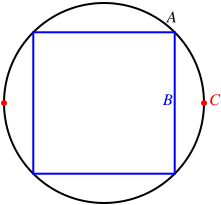
\includegraphics[width=\linewidth]{external/HM_Example.pdf}
\end{image}%
\tcblower
\end{figureptx}%
Determine \(h(A,B)\), \(h(A,C)\), and \(h(B,C)\), and verify that \(h(A,C) \leq h(A,B) + h(B,C)\).%
\item{}It may be surprising that \(h\) as in \hyperref[definition-def_Hausdorff_distance]{Definition~{\xreffont\ref{definition-def_Hausdorff_distance}}} is actually a metric, but it is. The underlying space is the collection of nonempty compact subsets of \(X\) which we denote at \(\mathcal{H}(X)\). Prove the following theorem.%
\begin{theorem}{Theorem}{}{}{theorem-sec_fractals-j-c-a-b}%
Let \(X\) be a metric space. The Hausdorff distance function is a metric on \(\mathcal{H}(X)\).%
\end{theorem}
\item{}One fun application of the Hausdorff metric is in fractal geometry. You may be familiar with objects like the Sierpinski triangle or the Koch curve. These objects are limits of sequences of sets in \(\mathcal{H}(\R^2)\). We illustrate with the Sierpinski triangle. Start with three points \(v_1\), \(v_2\), and \(v_3\) that form the vertices of an equilateral triangle  \(S_0\). For \(i\)=1,2, or 3, let \(v_i = \begin{bmatrix}a_i \\ b_i \end{bmatrix}\). For \(i\)=1,2, or 3, we define \(\omega_i : \R^2 \to \R^2\) by%
\begin{equation*}
\omega_i\left(\begin{bmatrix}x \\ y \end{bmatrix} \right) = \begin{bmatrix}\frac{1}{2} \amp  0 \\ 0 \amp  \frac{1}{2} \end{bmatrix} \begin{bmatrix}x \\ y \end{bmatrix}  + \begin{bmatrix}a_i \\ b_i \end{bmatrix}\text{.}
\end{equation*}
Then \(\omega_i\), when applied to \(S_0\), contracts \(S_0\) by a factor of 2 and then translates the image of \(S_0\) so that the \(i^{\text{ th } }\) vertex of \(S_0\) and the \(i\)th vertex of the image of \(S_0\) coincide. Such a map is called a \terminology{contraction mapping} with \terminology{contraction factor} equal to \(\frac{1}{2}\). Define \(S_{1,i}\) to be \(\omega_i(S_0)\). Then \(S_{1,i}\)  is the set of all points half way between any point in \(S_0\)  and  \(v_i\), or \(S_{1,i}\) is a triangle half the size of the original translated to the \(i^{\text{ th } }\) vertex of the original. Let \(S_1 = \bigcup_{i=1}^3 S_{1,i}\). Both \(S_0\) and \(S_1\) are shown in \hyperref[figure-F_Sierpinski]{Figure~{\xreffont\ref{figure-F_Sierpinski}}}. We can continue this procedure replacing \(S_0\) with \(S_1\). In other words, for \(i\) = 1, 2, and 3, let \(S_{2,i} = \omega_i(S_1)\). Then let \(S_2 = \bigcup_{i=1}^3 S_{2,i}\). A picture of \(S_2\) is shown in \hyperref[figure-F_Sierpinski]{Figure~{\xreffont\ref{figure-F_Sierpinski}}}. We can continue this procedure, each time replacing \(S_{j-1}\) with \(S_j\). A picture of \(S_8\) is shown in \hyperref[figure-F_Sierpinski]{Figure~{\xreffont\ref{figure-F_Sierpinski}}}.%
\begin{figureptx}{Figure}{\(S_i\) for \(i\) equal to 0, 1, 2, and 8.}{figure-F_Sierpinski}{}%
\centering
\begin{sidebyside}{2}{0}{0}{0}%
\begin{sbspanel}{0.5}%
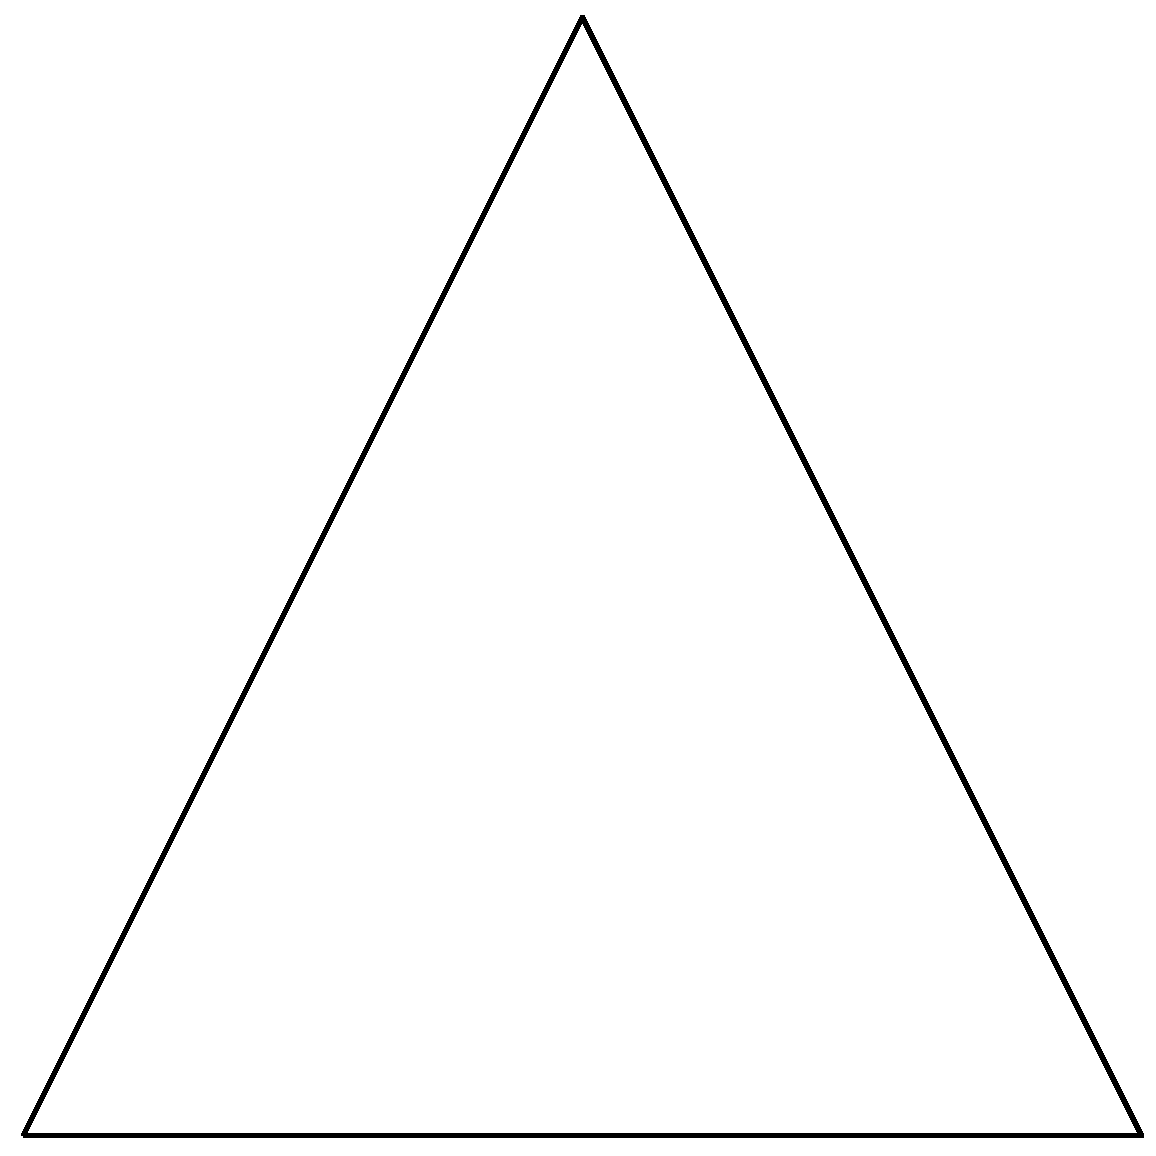
\includegraphics[width=\linewidth]{external/S0.pdf}
\end{sbspanel}%
\begin{sbspanel}{0.5}%
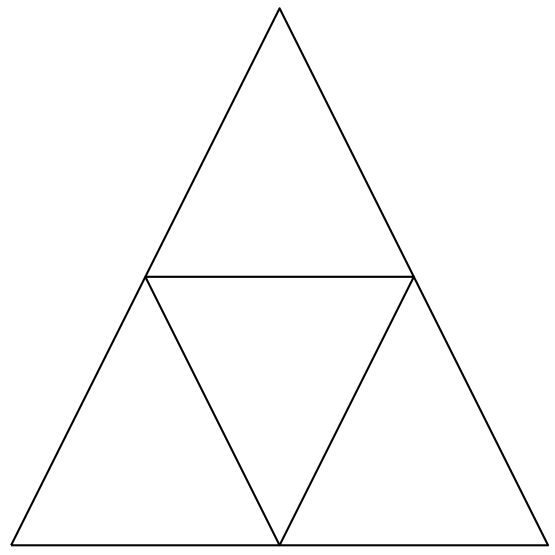
\includegraphics[width=\linewidth]{external/S1.pdf}
\end{sbspanel}%
\end{sidebyside}%
\begin{sidebyside}{2}{0}{0}{0}%
\begin{sbspanel}{0.5}%
%
\begin{equation*}
S_0
\end{equation*}
%
\end{sbspanel}%
\begin{sbspanel}{0.5}%
\par
%
\begin{equation*}
S_1
\end{equation*}
%
\end{sbspanel}%
\end{sidebyside}%
\begin{sidebyside}{2}{0}{0}{0}%
\begin{sbspanel}{0.5}%
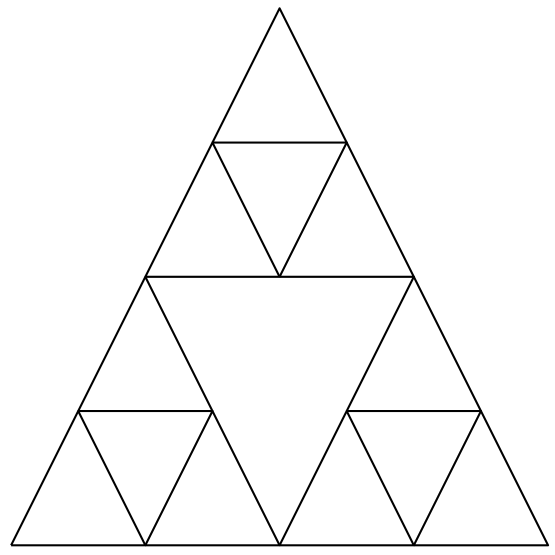
\includegraphics[width=\linewidth]{external/S2.pdf}
\end{sbspanel}%
\begin{sbspanel}{0.5}%
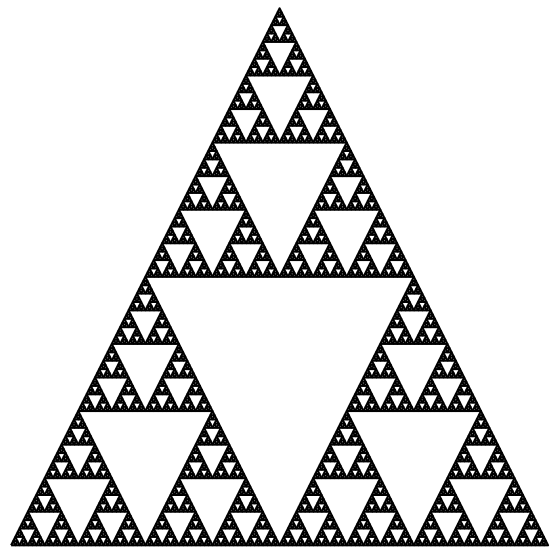
\includegraphics[width=\linewidth]{external/S8.pdf}
\end{sbspanel}%
\end{sidebyside}%
\begin{sidebyside}{2}{0}{0}{0}%
\begin{sbspanel}{0.5}%
%
\begin{equation*}
S_2
\end{equation*}
%
\end{sbspanel}%
\begin{sbspanel}{0.5}%
\par
%
\begin{equation*}
S_8
\end{equation*}
%
\end{sbspanel}%
\end{sidebyside}%
\tcblower
\end{figureptx}%
To continue this process, we need to take a limit. But the \(S_i\) are sets in \(\mathcal{H}(\R^2)\), so the limit is taken with respect to the Hausdorff metric.%
\begin{enumerate}[font=\bfseries,label=(\roman*),ref=\theenumi.\roman*]%
\item{}Assume that the length of a side of \(S_0\) is \(1\). Determine \(h(S_0,S_1)\). Then find \(h(S_k, S_{k+1})\) for an arbitrary positive integer \(k\).%
\item{}The Sierpinski triangle will exist if the sequence \((S_n)\) converges to a set \(S\) (which would be the Sierpinski triangle). The question of convergence is not a trivial one.%
\begin{enumerate}[font=\bfseries,label=(\Alph*),ref=\theenumi.\theenumii.\Alph*]%
\item{}Consider the sequence \((a_n)\), where \(a_n = \left(1+\frac{1}{n}\right)^n\) for \(n \in \Z^+\). Note that each \(a_n\) is a rational number. Explain why the terms in this sequence get arbitrarily close together, but the sequence does not converge in \(\Q\). Explain why the sequence \((a_n)\) converges in \(\R\).%
\item{}A sequence \((x_n)\) in a metric space \((X,d)\) is a \terminology{Cauchy sequence} if given \(\epsilon \gt 0\) there exists \(N \in \Z^+\) such that \(d(x_n, x_m) \lt \epsilon\) whenever \(n, m \geq N\). Every convergent sequence is a Cauchy sequence. A metric space \(X\) is said to be \terminology{complete}\index{metric space!complete} if every Cauchy sequence in \(X\) converges to an element in \(X\). For example, \((\R, d_E)\) is complete while \((\Q, d_E)\) is not. Although we will not prove it, the metric space \((\mathcal{H}(\R^2), h)\) is complete. Show that the sequence \((S_n)\) is a Cauchy sequence in \(\mathcal{H}(\R^2)\). The limit of this sequence is the famous Sierpinski triangle. The picture of \(S_8\) in \hyperref[figure-F_Sierpinski]{Figure~{\xreffont\ref{figure-F_Sierpinski}}} is a close approximation of the Sierpinski triangle.%
\end{enumerate}%
\end{enumerate}%
\end{enumerate}%
\end{activity}%
\end{sectionptx}
\end{chapterptx}
 %
%
\typeout{************************************************}
\typeout{Chapter 18 Connected Spaces}
\typeout{************************************************}
%
\begin{chapterptx}{Chapter}{Connected Spaces}{}{Connected Spaces}{}{}{chapter-chap_Connected_topology}
\renewcommand*{\chaptername}{Chapter}
\begin{objectives}{Focus Questions}{objectives-chap_Connected_topology-b}
%
\begin{itemize}[label=\textbullet]
\item{}What is a connected subset of a topological space?%
\item{}What is a separation of a subset of a topological space? Why are separations useful?%
\item{}What are the connected subsets of \(\R\)?%
\item{}What is a connected component of a topological space?%
\item{}What is an application of connectedness?%
\item{}What is a cut set of a topological space? Why are cut sets useful?%
\end{itemize}
\end{objectives}
%
%
\typeout{************************************************}
\typeout{Section  Introduction}
\typeout{************************************************}
%
\begin{sectionptx}{Section}{Introduction}{}{Introduction}{}{}{section-sec_connect_top_intro}
The term ``connected'' should bring up images of something that is one piece, not separated. There is more than one way we can interpret the notion of connectedness in topological spaces. For example, we might consider a topological space to be connected if we can't separate it into disjoint pieces in any non-trivial way. As another possibility, we might consider a topological space to be connected if there is always a path from one point in the spaced to another, provided we define what ``path'' means. These are different notions of connectedness, and we focus on the first notion in this section.%
\par
Connectedness is an important property, and one that we encounter in the calculus. For example, we will see in this section that the Intermediate Value Theorem relies on connected subsets of \(\R\). To define a connected set, we will need to have a way to understand when and how a set can be separated into different pieces. Since a topology is defined by open sets, when we want to separate objects we will do so with open sets. This is similar to the idea behind Hausdorff spaces, except that we now want to know if a set can be separated in some way rather than separating points.%
\par
As an example to motivate the definition, consider the sets \(X = (0,1) \cup (1,2)\) and \(Y = [1,2]\) in \(\R\) with the Euclidean topology. Notice that we can write \(X\) as the union of two disjoint open sets \(X_1 = (0,1)\) and \(X_2 = (1,2)\). So we shouldn't think of \(X\) as being connected. However, if we attempt to write \(Y\) as a union of two subsets, say \(Y_1 = [1,1.5)\) and \(Y_2 = [1.5,2]\), it is impossible for both of these subsets to be open and disjoint. So \(Y\) is a set we should consider to be connected. This is the notion of connectedness that we wish to investigate.%
\begin{definition}{Definition}{}{definition-sec_connect_top_intro-e}%
\index{connected space}%
A topological space \((X,\tau)\) is \terminology{connected} if \(X\) cannot be written as the union of two disjoint, nonempty, open subsets. A subset \(A\) of a topological space topological space \((X,\tau)\) is connected if \(A\) is connected in the subspace topology.%
\end{definition}
If a set \(X\) is not connected, we say that \(X\) is disconnected. If \(X\) is a disconnected topological space, then there exist disjoint nonempty open sets \(U\) and \(V\) such that \(X = U \cup V\).%
\begin{exploration}{Preview Activity}{}{exploration-sec_connect_top_intro-g}%
Can the subset \(A\) of the topological space \(X\) be written as the union of two disjoint nonempty relatively open sets?%
\begin{enumerate}[font=\bfseries,label=(\alph*),ref=\alph*]%
\item{}The set \(A = \{a, b\}\) in \((X, \tau)\) with \(X = \{a, b, c, d\}\) and \(\tau = \{\emptyset, \{a\}, \{b\}, \{a, b\}, X\}\).%
\item{}The set \(A = \{a, b, c\}\) in \((X, \tau)\) with \(X = \{a,b,c,d,e,f\}\) and%
\begin{equation*}
\tau = \{\emptyset, \{a\}, \{c,d\}, \{a, c, d\}, \{b,c,d,e,f\}, X\}\text{.}
\end{equation*}
%
\item{}The set \(A = X\) with \(X = \{a,b,c,d\}\) and%
\begin{equation*}
\tau = \{\emptyset, \{b\}, \{c\}, \{a,b\}, \{b,c\}, \{a,b,c\}, \{b,c,d\}, X\}\text{.}
\end{equation*}
%
\item{}The set \(A = \{d, f\}\) in \(X = \{a, b, c, d, e, f\}\) with the discrete topology. Generalize your findings.%
\item{}The set \(A = \{a, c, d\}\) in \(X = \{a, b, c, d, e\}\) with the indiscrete topology. Generalize your findings.%
\item{}The set \(A = \Z\) in \(X = \R\) with the finite complement topology. Generalize your findings.%
\item{}The set \(A = X\) in \(X = \{x \in \R \ \mid \ 1 \leq x \leq 2 \text{ or } 3 \lt x \lt 4\}\) with the subspace metric topology from \((\R, d_E)\).%
\item{}The set \(A = X\) in \(X = \left\{(x, y) \in \R^2 \ \mid \  y = \frac{1}{x} \text{ or }  y = 0\right\}\) with open sets%
\begin{equation*}
\tau = \{U  \cap X \ \mid \ U \text{ is open in the Euclidean Topology on }  \R^2\}\text{.}
\end{equation*}
%
\end{enumerate}%
\end{exploration}%
\end{sectionptx}
%
%
\typeout{************************************************}
\typeout{Section  Connected Sets}
\typeout{************************************************}
%
\begin{sectionptx}{Section}{Connected Sets}{}{Connected Sets}{}{}{section-sec_connect_sets}
As we learned in our preview activity, connected sets are those sets that cannot be separated into a union of disjoint open sets. Another characterization of connectedness is established in the next activity.%
\begin{activity}{Activity}{}{activity-sec_connect_sets-c}%
Let \((X, \tau)\) be a topological space.%
\begin{enumerate}[font=\bfseries,label=(\alph*),ref=\alph*]%
\item{}Assume that \(X\) is a connected space, and let \(A\) be a subset of \(X\) that is both open and closed. What happens if we combine \(A\) and \(X \setminus A\)? What does the fact that \(X\) is connected tell us about \(A\)?%
\item{}Now assume that the only subsets of \(X\) that are both open and closed are \(\emptyset\) and \(X\). Must it follow that \(X\) is connected? Prove your assertion.%
\item{}Summarize the result of this activity into a theorem of the form ``A topological space \((X, \tau)\) is connected if and only if ...''.%
\end{enumerate}%
\end{activity}%
A standard example of a connected topological space is the metric space \((\R, d_E)\).%
\begin{theorem}{Theorem}{}{}{theorem-thm_R_connected}%
The metric space \((\R, d_E)\) is a connected topological space.%
\end{theorem}
\begin{proof}{Proof}{}{proof-thm_R_connected-b}
We proceed by contradiction and assume that there are nonempty open sets \(U\) and \(V\) such that \(\R = U \cup V\) and \(U \cap V = \emptyset\). Let \(a \in U\) and \(b \in V\). Since \(U \cap V = \emptyset\), we know that \(a \neq b\). Without loss of generality we can assume \(a \lt b\). Let \(U' = U \cap [a,b]\) and let \(V' = V \cap [a,b]\). The set \(V'\) is bounded below by \(a\), so \(x = \inf\{v \mid v \in V'\}\) exists. Since \(\R = U \cup V\) it must be the case that \(x \in U\) or \(x \in V\).%
\par
Suppose \(x \in U\). The fact that \(U\) is an open set implies that there exists \(\epsilon \gt 0\) such that \(B(x, \epsilon) \subseteq U\). But then \(B(x, \epsilon) \cap V = \emptyset\) and so \(d(x,v) \geq \epsilon\) for every \(v \in V\). This means that \(x+\epsilon \lt v\) for every \(v \in V'\), contradicting the fact that \(x\) is the greatest lower bound. We conclude that \(x \notin U\).%
\par
It follows that \(x \in V\). Since \(a \in U\), we know that \(x \neq a\). The fact that \(V\) is an open set tells us that there exists \(\delta \gt 0\) such that \(B(x, \delta) \subseteq V\). We can choose \(\delta\) to ensure that \(\delta \lt x-a\). Since \(x > a\), the interval \((x-\delta,
x)\) is a subset of \(V'\), and so \(x\) is not a lower bound for \(V\).%
\par
Each possibility leads to a contradiction, so we conclude that the sets \(U\) and \(V\) cannot exist. Therefore, \((\R, d_E)\) is a connected topological space.%
\end{proof}
As you might expect, connectedness is a topological property.%
\begin{activity}{Activity}{}{activity-sec_connect_sets-g}%
Let \((X, \tau_X)\) and \((Y, \tau_Y)\) be topological spaces, and let \(f : X \to Y\) be a continuous function. Assume that \(X\) is a connected subset of \(X\). Our goal is to prove that \(f(X)\) is a connected subspace of \(Y\).%
\par
Let \(Z = f(X)\) and define \(g: X \to Z\) by \(g(x) = f(x)\). Then \(g\) is a continuous function that maps \(X\) onto \(Z\). So we consider \(g\) instead of \(f\).%
\begin{enumerate}[font=\bfseries,label=(\alph*),ref=\alph*]%
\item{}Assume to the contrary that \(Z\) is not connected. What do we then assume about \(Z\)?%
\item{}Suppose that \(U\) and \(V\) are disjoint nonempty open sets in \(Z\) such that \(U \cup V = Z\). Let \(R = g^{-1}(U)\) and \(S = g^{-1}(V)\).%
\begin{enumerate}[font=\bfseries,label=(\roman*),ref=\theenumi.\roman*]%
\item{}Explain why \(R\) and \(S\) are open sets in \(X\).%
\item{}Show that \(R \cup S = X\). (Hint: \(X = g^{-1}(Z)\).)%
\item{}Show \(R\) and \(S\) are nonempty sets.%
\par\smallskip%
\noindent\textbf{\blocktitlefont Hint}.\hypertarget{hint-sec_connect_sets-g-c-d-b}{}\quad{}Use the fact that \(g\) is a surjection.%
\item{}Now show that \(R \cap S = \emptyset\). (Hint: \(R \cap S = g^{-1}(U) \cap g^{-1}(V)\).)%
\end{enumerate}%
\item{}Explain how we have proved the following.%
\begin{theorem}{Theorem}{}{}{theorem-thm_connected_invariant}%
Let \((X, \tau_X)\) and \((Y, \tau_Y)\) be topological spaces, and let \(f : X \to Y\) be a continuous function. If \(X\) is connected, then \(f(X)\) is connected.%
\end{theorem}
\end{enumerate}%
\end{activity}%
The fact that connectedness is preserved by continuous functions means that connectedness is a property that is shared by any homeomorphic topological spaces, as the next corollary indicates.%
\begin{corollary}{Corollary}{}{}{corollary-sec_connect_sets-i}%
Let \((X, \tau_X)\) and \((Y, \tau_Y)\) be homeomorphic topological spaces. Then \(X\) is connected if and only if \(Y\) is connected.%
\end{corollary}
\begin{proof}{Proof}{}{proof-sec_connect_sets-i-b}
Let \((X, \tau_X)\) and \((Y, \tau_Y)\) be topological spaces and let \(f: X \to Y\) be a homeomorphism. Assume that \(X\) is connected. Since \(f\) is continuous, \hyperref[theorem-thm_connected_invariant]{Theorem~{\xreffont\ref{theorem-thm_connected_invariant}}} shows that \(f(X) = Y\) is connected. The reverse implication follows from the fact that \(f^{-1}\) is a homeomorphism.%
\end{proof}
Recall that \((\R,d_E)\) is homeomorphic to the topological subspaces \((a,b)\), \((-\infty,
b)\), and \((a,\infty)\) for any \(a, b \in \R\). The fact that \((\R, d_E)\) is connected (\hyperref[theorem-thm_R_connected]{Theorem~{\xreffont\ref{theorem-thm_R_connected}}}) allows us to conclude that all open intervals are connected. It would seem natural that all closed (or half-closed) intervals should also be connected. We address this question next. Before we get to this result, we consider an alternate formulation of connected subsets.%
\par
Consider the set \(A = (-1,0) \cup (4,5)\) in \(\R\). Let \(U = (-2,3)\) and \(V=(2,6)\) in \(\R\). Note that \(U' = U \cap A = (-1,0)\) and \(V' = V \cap A = (4,5)\), and so \(U\) and \(V\) are open sets in \(\R\) that separate the set \(A\) into two disjoint pieces. We know that \(U'\) and \(V'\) are open in \(A\) and \(A = U' \cup V'\) with \(U' \cap V' = \emptyset\). So to show that a subset of a topological space \(X\) is not connected, this example suggests that it suffices to find nonempty open sets \(U\) and \(V\) in \(X\) with \(U \cap V \cap A = \emptyset\) and \(A \subseteq (U \cup V)\). Note that it is not necessary to have \(U \cap V = \emptyset\). That this works in general is the result of the next theorem.%
\begin{theorem}{Theorem}{}{}{theorem-thm_conn_subset}%
Let \(X\) be a topological space. A subset \(A\) of \(X\) is disconnected if and only if there exist open sets \(U\) and \(V\) in \(X\) with%
\begin{itemize}[label=\textbullet]
\item{}\(A \subseteq (U \cup V)\),%
\item{}\(U \cap A \neq \emptyset\),%
\item{}\(V \cap A \neq \emptyset\), and%
\item{}\(U \cap V \cap A = \emptyset\).%
\end{itemize}
%
\end{theorem}
\begin{proof}{Proof}{}{proof-thm_conn_subset-b}
Let \(X\) be a topological space, and let \(A\) be a subset of \(X\). We first assume that \(A\) is disconnected and show that there are open sets \(U\) and \(V\) in \(X\) that satisfy the given conditions. Since \(A\) is disconnected, there are nonempty open sets \(U'\) and \(V'\) in \(A\) such that \(U' \cup V' = A\) and \(U' \cap V' = \emptyset\). Since \(U'\) and \(V'\) are open in \(A\), there exist open sets \(U\) and \(V\) in \(X\) so that \(U' = U \cap A\) and \(V' = V \cap A\). Now%
\begin{equation*}
A = U' \cup V' = (U \cap A) \cup (V \cap A) = (U \cup V) \cap A\text{,}
\end{equation*}
and so \(A \subseteq U \cup V\). By construction, \(U \cap A = U'\) and \(V \cap A = V'\) are not empty. Finally,%
\begin{equation*}
U \cap V \cap A = (U \cap A) \cap (V \cap A) = U' \cap V' = \emptyset\text{.}
\end{equation*}
%
\par
So we have found sets \(U\) and \(V\) that satisfy the conditions of our theorem.%
\par
The proof of the reverse implication is left to the next activity.%
\end{proof}
\begin{activity}{Activity}{}{activity-sec_connect_sets-m}%
Let \(X\) be a topological space, and let \(A\) be a subset of \(X\). Assume that there exist open sets \(U\) and \(V\) in \(X\) with \(A \subseteq U \cup V\), \(U \cap A \neq \emptyset\), \(V \cap A \neq \emptyset\), and \(U \cap V \cap A = \emptyset\). Prove that \(A\) is disconnected.%
\end{activity}%
The conditions in \hyperref[theorem-thm_conn_subset]{Theorem~{\xreffont\ref{theorem-thm_conn_subset}}} provide a convenient way to show that a set is disconnected, and so any pair of sets \(U\) and \(V\) that satisfy the conditions of \hyperref[theorem-thm_conn_subset]{Theorem~{\xreffont\ref{theorem-thm_conn_subset}}} is given a special name.%
\begin{definition}{Definition}{}{definition-sec_connect_sets-o}%
\index{separation}%
Let \(X\) be a topological space, and let \(A\) be a subset of \(X\). A \terminology{separation} of \(A\) is a pair of nonempty open subsets \(U\) and \(V\) of \(X\) such that%
\begin{itemize}[label=\textbullet]
\item{}\(A \subseteq (U \cup V)\),%
\item{}\(U \cap A \neq \emptyset\),%
\item{}\(V \cap A \neq \emptyset\), and%
\item{}\(U \cap V \cap A = \emptyset\).%
\end{itemize}
%
\end{definition}
If \(X\) is a disconnected topological space, then a separation of \(X\) is a pair \(U\), \(V\) of disjoint nonempty open sets such that \(U \cup V = X\).%
\end{sectionptx}
%
%
\typeout{************************************************}
\typeout{Section  Connected Subsets of \(\R\)}
\typeout{************************************************}
%
\begin{sectionptx}{Section}{Connected Subsets of \(\R\)}{}{Connected Subsets of \(\R\)}{}{}{section-sec_connect_subset_rn}
With \hyperref[theorem-thm_conn_subset]{Theorem~{\xreffont\ref{theorem-thm_conn_subset}}} in hand, we are just about ready to show that any interval in \(\R\) is connected. Let us return for a moment to our example of \(A = (-1,0) \cup (4,5)\) in \(\R\). It is not difficult to see that if \(U\) and \(V\) are a separation of \(A\), then the subset \((-1,0)\) must be entirely contained in either \(U\) or in \(V\). The reason for this is that \((-1,0)\) is a connected subset of \(A\). This result is true in general.%
\begin{activity}{Activity}{}{activity-sec_connect_subset_rn-c}%
Let \(X\) be a topological space, and let \(A\) be a subset of \(X\). Assume that \(U\) and \(V\) form a separation of \(A\). Let \(C\) be a connected subset of \(A\). In this activity we want to prove that \(C \subseteq U\) or \(C \subseteq V\).%
\begin{enumerate}[font=\bfseries,label=(\alph*),ref=\alph*]%
\item{}Use the fact that \(U\) and \(V\) form a separation to \(A\) to wxplain why \(C \subseteq U \cup V\) and \(C \cap U \cap V = \emptyset\).%
\item{}Given that \(C\) is connected, what conclusion can we draw about the sets \(U' = U \cap C\) and \(V' = V \cap C\)?%
\item{}Complete the proof of the following lemma.%
\begin{lemma}{Lemma}{}{}{lemma-lem_separation_subset}%
Let \(X\) be a topological space, and let \(A\) be a subset of \(X\). Assume that \(U\) and \(V\) form a separation of \(A\). If \(C\) is a connected subset of \(A\), then \(C \subseteq U\) or \(C \subseteq V\).%
\end{lemma}
\end{enumerate}%
\end{activity}%
Now we can prove that any interval in \(\R\) is connected. Since \([a,b]\), \([a,b)\), and \((a,b]\) are all sets that lie between \((a,b)\) and \(\overline{(a,b)}\), we can address their connectedness all at once with the next result.%
\begin{theorem}{Theorem}{}{}{theorem-thm_connected_limitpoints}%
Let \(X\) be a topological space and \(C\) a connected subset of \(X\). If \(A\) is a subset of \(X\) and \(C \subseteq A \subseteq \overline{C}\), then \(A\) is connected in \(X\).%
\end{theorem}
\begin{proof}{Proof}{}{proof-thm_connected_limitpoints-b}
Let \(X\) be a topological space and \(C\) a connected subset of \(X\). Let \(A\) be a subset of \(X\) such that \(C \subseteq A \subseteq \overline{C}\). To show that \(A\) is connected, assume to the contrary that \(A\) is disconnected. Then there are nonempty open subsets \(U\) and \(V\) of \(X\) that form a separation of \(A\). \hyperref[lemma-lem_separation_subset]{Lemma~{\xreffont\ref{lemma-lem_separation_subset}}} shows that \(C \subseteq U\) or \(C \subseteq V\). Without loss of generality we assume that \(C \subseteq U\). Since \(U \cap V \cap A = \emptyset\), it follows that%
\begin{equation*}
C \cap V = (C \cap A) \cap V = C \cap (A \cap V)  \subseteq U \cap A \cap V = \emptyset\text{.}
\end{equation*}
%
\par
Since \(A \cap V \neq \emptyset\), there is an element \(x \in A \cap V\). Since \(x \notin C\) and \(x \in A \subseteq \overline{C}\), it must be the case that \(x\) is a limit point of \(C\). Since \(V\) is an open neighborhood of \(x\), it follows that \(V \cap C \neq \emptyset\). This contradiction allows us to conclude that \(A\) is connected.%
\end{proof}
One consequence of \hyperref[theorem-thm_connected_limitpoints]{Theorem~{\xreffont\ref{theorem-thm_connected_limitpoints}}} is that any interval of the form \([a,b)\), \((a,b]\), \([a,b]\), \((-\infty,
b]\), or \([a, \infty)\) in \(\R\) is connected. This prompts the question, are there any other subsets of \(\R\) that are connected?%
\begin{activity}{Activity}{}{activity-act_connected_subsets_R}%
Let \(A\) be a subset of \(\R\).%
\begin{enumerate}[font=\bfseries,label=(\alph*),ref=\alph*]%
\item{}Let \(A = \{a\}\) be a single point subset of \(\R\). Is \(A\) connected? Explain.%
\item{}Now suppose that \(A\) is a subset of \(\R\) that contains two or more points. Assume that \(A\) is not an interval. Then there must exist points \(a\) and \(b\) in \(A\) and a point \(c\) in \(\R \setminus A\) between \(a\) and \(b\). Use this idea to find a separation of \(A\). What can we conclude about \(A\)?%
\item{}Explicitly describe the connected subsets of \((\R, d_E)\).%
\end{enumerate}%
\end{activity}%
\end{sectionptx}
%
%
\typeout{************************************************}
\typeout{Section  Components}
\typeout{************************************************}
%
\begin{sectionptx}{Section}{Components}{}{Components}{}{}{section-sec_components}
As \hyperref[activity-act_connected_subsets_R]{Activity~{\xreffont\ref{activity-act_connected_subsets_R}}} demonstrates, spaces like \(A = (1,2) \cup (3,4)\) are not connected. Even so, \(A\) is made of two connected subsets \((1,2)\) and \((3,4)\). These connected subsets are called \terminology{components}.%
\begin{definition}{Definition}{}{definition-sec_components-c}%
\index{component}%
A subspace \(C\) of a topological space \(X\) is a \terminology{component} (or \terminology{connected component}) of \(X\) if \(C\) is connected and there is no larger connected subspace of \(X\) that contains \(C\).%
\end{definition}
As an example, if \(X = (1,2) \cup [4,10) \cup \{-1,15\}\), then the components of \(X\) are \((1,2)\), \([4,10)\), \(\{-1\}\) and \(\{15\}\). As the next activity shows, we can always partition a topological space into a disjoint union of compenents.%
\begin{activity}{Activity}{}{activity-act_connected_compenent}%
Let \((X, \tau)\) be a nonempty topological space.%
\begin{enumerate}[font=\bfseries,label=(\alph*),ref=\alph*]%
\item{}Show that if \(x \in X\), then \(\{x\}\) is connected.%
\item{}Suppose that \(X\) is a topological space and \(\{A_{\alpha}\}\) for \(\alpha\) in some indexing set \(I\) is a collection of connected subsets of \(X\). Let \(A = \bigcup_{\alpha \in I} A_{\alpha}\). Suppose that \(\bigcap_{\alpha \in I} A_{\alpha} \neq \emptyset\). Show that \(A\) is a connected subset of \(X\).%
\par\smallskip%
\noindent\textbf{\blocktitlefont Hint}.\hypertarget{hint-act_connected_compenent-c-b}{}\quad{}Assume a separation and use \hyperref[lemma-lem_separation_subset]{Lemma~{\xreffont\ref{lemma-lem_separation_subset}}}.%
\item{}Part (a) shows that every element in \(x\) belongs to some connected subset of \(X\). So we can write \(X\) as a union of connected subsets. But there is probably overlap. To remove the overlap, we define the following relation \(\sim\) on \(X\): For \(x\) and \(y\) in \(X\), \(x \sim y\) if \(x\) and \(y\) are contained in the same connected subset of \(X\). As with any relation, we ask if \(\sim\) is an equivalence relation.%
\begin{enumerate}[font=\bfseries,label=(\roman*),ref=\theenumi.\roman*]%
\item{}Is \(\sim\) a reflexive relation? Why or why not?%
\item{}Is \(\sim\) a symmetric relation? Why or why not?%
\item{}Is \(\sim\) a transitive relation? Why or why not?%
\end{enumerate}%
\end{enumerate}%
\end{activity}%
\hyperref[activity-act_connected_compenent]{Activity~{\xreffont\ref{activity-act_connected_compenent}}} shows that the relation \(\sim\) is an equivalence relation, and so partitions the underlying topological space \(X\) into disjoint sets. If \(x \in X\), then the equivalence class of \(x\) is a connected subset of \(X\). There can be no larger connected subset of \(X\) that contains \(x\), since equivalence classes are disjoint or the same. So the equivalence classes are exactly the connected components of \(X\). The components of a topological space \(X\) satisfy several properties.%
\begin{itemize}[label=\textbullet]
\item{}Each \(a \in X\) is an element of exactly one connected component \(C_a\) of \(X\).%
\item{}A component \(C_a\) contains all connected subsets of \(X\) that contain \(a\). Thus, \(C_a\) is the union of all connected subsets of \(X\) that contain \(a\).%
\item{}If \(a\) and \(b\) are in \(X\), then either \(C_a = C_b\) or \(C_a \cap C_b = \emptyset\).%
\item{}Every connected subset of \(X\) is a subset of a connected component.%
\item{}Every connected component of \(X\) is a closed subset of \(X\).%
\item{}The space \(X\) is connected if and only if \(X\) has exactly one connected component.%
\end{itemize}
%
\end{sectionptx}
%
%
\typeout{************************************************}
\typeout{Section  Cut Sets}
\typeout{************************************************}
%
\begin{sectionptx}{Section}{Cut Sets}{}{Cut Sets}{}{}{section-sec_cut_sets}
It can be difficult to determine if two topological spaces are homeomorphic. We can sometimes use topological invariants to determine if spaces are not homeomorphic. For example, if \(X\) is connected and \(Y\) is not, then \(X\) and \(Y\) are not homeomorphic. But just because two spaces are connected, it does not automatically follow that the spaces are homeomorphic. For example consider the spaces \((0,2)\) and \([0,2)\). Both are connected subsets of \(\R\). If we remove a point, say 1, from the set \((0,2)\) the resulting space \((0,1) \cup (1,2)\) is no longer connected. The same result is true if we remove any point from \((0,2)\). However, if we remove the point \(0\) from \([0,2)\) the resulting space \((0,2)\) is connected. So the spaces \((0,2)\) and \([0,2)\) are fundamentally different in this respect, and so are not homeomorphic. Any set that we can remove from a connected set to obtain a disconnected set is called a \terminology{cut set}.%
\begin{definition}{Definition}{}{definition-sec_cut_sets-c}%
\index{cut set}%
\index{cut point}%
A subset \(S\) of a connected topological space \(X\) is a \terminology{cut set} of \(X\) if the set \(X \setminus S\) is disconnected. A point \(p\) in a connected topological space \(X\) is a \terminology{cut point} if \(X \setminus \{p\}\) is disconnected.%
\end{definition}
\begin{example}{Example}{}{example-sec_cut_sets-d}%
\begin{enumerate}[font=\bfseries,label=(\alph*),ref=\alph*]%
\item{}The point \(1\) is a cut point of the space \((0,2)\). In fact, every point in \((0,2)\) is a cut point of \((0,2)\).%
\item{}Let \(D = \{(x,y) \mid x^2+y^2 \leq 4\}\) in \((\R^2, d_E)\). That is, \(D\) is the closed disk of radius \(2\) in the plane. The set \(D\) has no cut points. However, if \(S = \{(x,y) \mid x^2+y^2 = 1\}\), then \(D \setminus S\) consists of two connected components: the open ball \(B((0,0),1)\) and the annulus \(\{(x,y) \mid 1 \lt x^2+y^2 \leq 4\}\) as illustrated in \hyperref[figure-F_Cut_set_disk]{Figure~{\xreffont\ref{figure-F_Cut_set_disk}}}. So \(S\) is a cut set of \(D\).%
\begin{figureptx}{Figure}{The disk \(D\) and cut set \(S\).}{figure-F_Cut_set_disk}{}%
\begin{image}{0.25}{0.5}{0.25}{}%
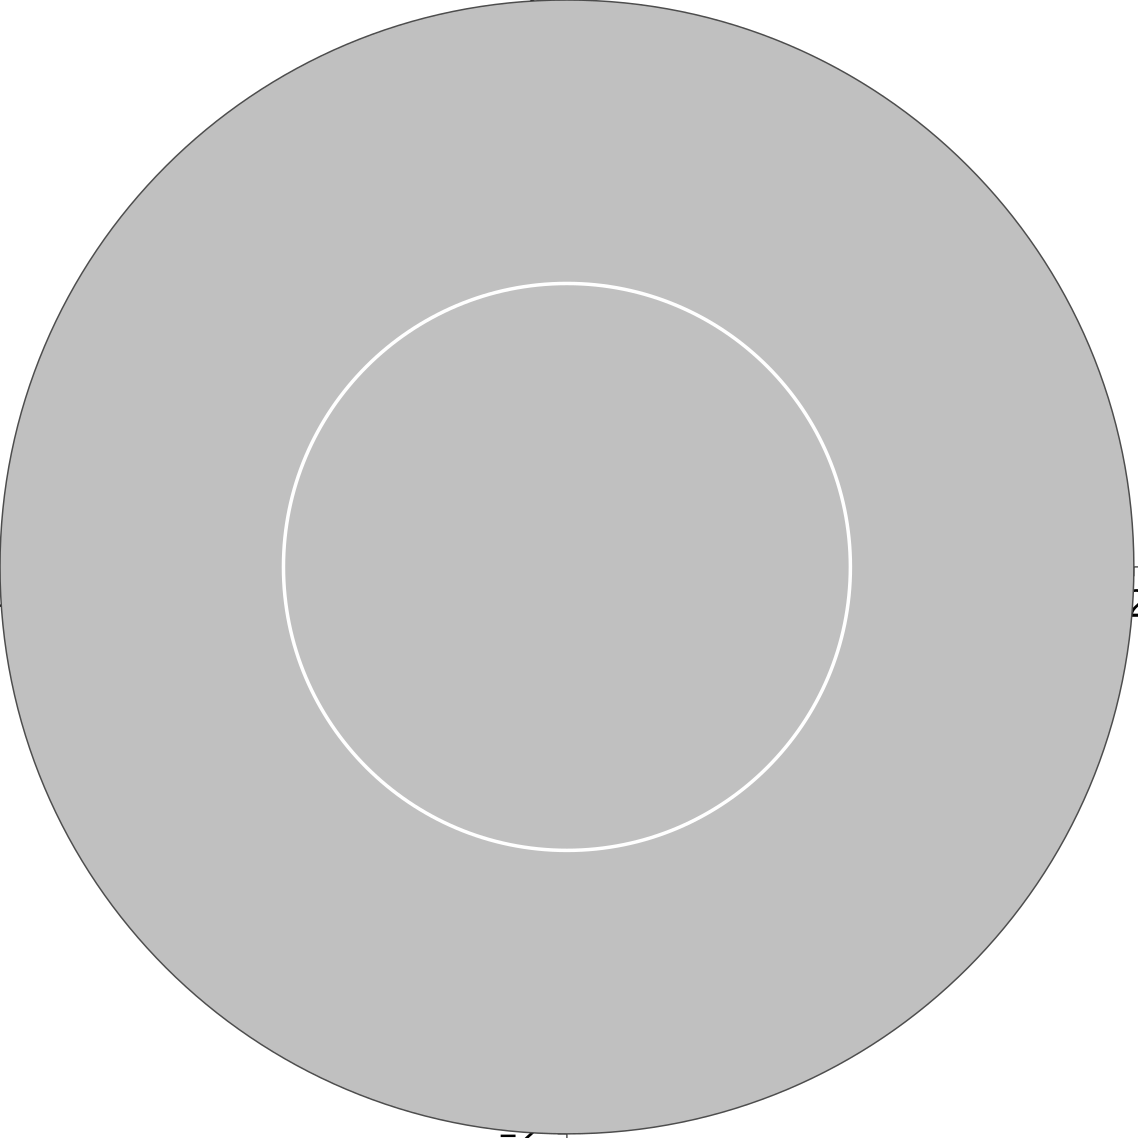
\includegraphics[width=\linewidth]{external/Cut_set_disk.pdf}
\end{image}%
\tcblower
\end{figureptx}%
\end{enumerate}%
\end{example}
Once we have a new property, we then ask if that property is a topological invariant.%
\begin{theorem}{Theorem}{}{}{theorem-sec_cut_sets-f}%
Let \(X\) and \(Y\) be connected topological spaces and let \(f:X \to Y\) be a homeomorphism. If \(S \subset X\) is a cut set, then \(f(S)\) is a cut set of \(Y\).%
\end{theorem}
\begin{proof}{Proof}{}{proof-sec_cut_sets-f-b}
Let \(X\) and \(Y\) be topological spaces with \(f : X \to Y\) a homeomorphism. Let \(S\) be a cut set of \(X\). Let \(U\) and \(V\) form a separation of \(X \setminus S\). We will demonstrate that \(f(U)\) and \(f(V)\) form a separation of \(Y \setminus f(S)\), which will prove that \(f(S)\) is a cut set of \(Y\). Since \(f^{-1}\) is continuous, the sets \(f(U)\) and \(f(V)\) are open sets in \(Y\). Next we prove that \((Y \setminus f(S)) \subseteq (f(U) \cup f(V))\). Let \(y \in Y \setminus f(S)\). Since \(f\) is a surjection, there exists an \(x \in X\) with \(f(x) = y\). The fact that \(y \notin f(S)\) means that \(x \notin S\). So \(x \in (X \setminus S) \subseteq (U \cup V)\). If \(x \in U\), then \(f(x) = y \in f(U)\) and if \(x \in V\), then \(x = f(y) \in f(V)\). So \((Y \setminus f(S)) \subseteq (f(U) \cup f(V))\).%
\par
Now we demonstrate that \(f(U) \cap (Y \setminus f(S)) \neq \emptyset\) and \(f(V) \cap (Y \setminus f(S)) \neq \emptyset\). Since \(U\) and \(V\) form a separation of \(X \setminus S\), we know that \(U \cap (X \setminus S) \neq \emptyset\) and \(V \cap (X \setminus S) \neq \emptyset\). Let \(x \in U \cap (X \setminus S)\). Then \(x \in U\) and \(x \notin S\). So \(f(x) \in f(U)\) and the fact that \(f\) is an injection implies that \(f(x) \notin f(S)\). Thus, \(f(x) \in f(U) \cap (Y \setminus f(S))\). The same argument shows that \(x \in V \cap (X \setminus S)\) implies that \(f(x) \in f(V) \cap (Y \setminus f(S))\). So \(f(U) \cap (Y \setminus f(S)) \neq \emptyset\) and \(f(V) \cap (Y \setminus f(S)) \neq \emptyset\).%
\par
Finally, we show that \(f(U) \cap f(V) \cap (Y \setminus f(S)) = \emptyset\). Suppose \(y \in f(U) \cap f(V) \cap (Y \setminus f(S))\). Let \(x \in X\) such that \(f(x) = y\). Since \(f\) is an injection, we know that \(f(x) \in f(U)\) means \(x \in U\). so \(x \in U \cap V\). The fact that \(y \in Y \setminus f(S)\) means that \(y \notin f(S)\). Thus, \(x \notin S\). So \(x \in X \setminus S\). We then have \(x \in U \cap V \cap (X \setminus S) = \emptyset\). It follows that \(f(U) \cap f(V) \cap (Y \setminus f(S)) = \emptyset\). Therefore, \(f(U)\) and \(f(V)\) form a separation of \(Y \setminus f(S)\) and \(f(S)\) is a cut set of \(Y\).%
\end{proof}
\begin{activity}{Activity}{}{activity-sec_cut_sets-g}%
\begin{enumerate}[font=\bfseries,label=(\alph*),ref=\alph*]%
\item{}Use the idea of cut sets\slash{}points to explain why the unit circle in \(\R^2\) is not homeomorphic to the interval \([0,1]\) in \(\R\). Note: the unit circle is the set \(\{(x,y) \mid x^2+y^2 = 1\}\). Draw pictures to illustrate your explanation. (A formal proof is not necessary, but you need to provide a convincing justification.)%
\item{}Consider the following subsets of \(\R^2\) in the subspace topology:%
\begin{equation*}
A = \{ (x,y) \mid x^2+y^2 =1\} \ \ \ \text{ and }  \ \ \ B = \{ (x,0) \mid -1 \leq x \leq 1\}\text{.}
\end{equation*}
Is \(A \cup B\) homeomorphic to \(A\)? (A formal proof is not necessary, but you need to provide a convincing justification.)%
\end{enumerate}%
\end{activity}%
We have seen that topological equivalence is an equivalence relation, which partitions the collection of all topological spaces into disjoint homeomorphism classes. Topological invariants can then help us identify the classes to which different spaces belong. In general, though, it can be more difficult to prove that two spaces are homeomorphic than not homeomorphic.%
\begin{activity}{Activity}{}{activity-sec_cut_sets-i}%
Consider the spaces \(S_1 = \R\), \(S_2 = (0,1)\) in \(\R\), \(S_3 = [-1,1]\) in \(\R\), the line segment \(S_4\) in \(\R^2\) between the points \((0,0)\) and \((2,2)\), the space \(S_5\) determined by the letter \textbraceleft{} X\textbraceright{}, and the space \(S_6\) determined by the letter \textbraceleft{} Y\textbraceright{} in \(\R^2\). Identify the distinct homeomorphism classes determined by these six spaces. No formal proofs are necessary, but you need to give convincing arguments.%
\end{activity}%
\end{sectionptx}
%
%
\typeout{************************************************}
\typeout{Section  The Intermediate Value Theorem and a Fixed Point Theorem}
\typeout{************************************************}
%
\begin{sectionptx}{Section}{The Intermediate Value Theorem and a Fixed Point Theorem}{}{The Intermediate Value Theorem and a Fixed Point Theorem}{}{}{section-sec_ivt_fpt}
In this section we present two important consequences of connectedness. The first consequence is the Intermediate Value Theorem. In calculus, the Intermediate Value Theorem tells us that if \(f\) is a continuous function on a closed interval \([a,b]\), then \(f\) assumes all values between \(f(a)\) and \(f(b)\). This result seems straightforward if one just draws a graph of a continuous function on a closed interval. But a picture is not a proof. We state and then prove a more general version of the Intermediate Value Theorem.%
\begin{theorem}{Theorem}{The Intermediate Value Theorem.}{}{theorem-sec_ivt_fpt-c}%
Let \(X\) be a topological space and \(A\) a connected subset of \(X\). If \(f : A \to \R\) is a continuous function, then for any \(a,b \in A\) and any \(y \in \R\) between \(f(a)\) and \(f(b)\), there is a point \(x \in A\) such that \(f(x) = y\).%
\end{theorem}
\begin{activity}{Activity}{}{activity-sec_ivt_fpt-d}%
In this activity we prove the Intermediate Value Theorem. Let \(X\) be a topological space and \(A\) a connected subset of \(X\). Assume that \(f : A \to \R\) is a continuous function, and let \(a,b \in A\).%
\begin{enumerate}[font=\bfseries,label=(\alph*),ref=\alph*]%
\item{}Explain why we can assume that \(a \neq b\).%
\item{}Explain what happens if \(y = f(a)\) or \(y=f(b)\).%
\item{}Now assume that \(f(a) \neq f(b)\). Without loss of generality, assume that \(f(a) \lt f(b)\). Why can we say that \(f(A)\) is an interval?%
\item{}How does the fact that \(f(A)\) is an interval complete the proof?%
\end{enumerate}%
\end{activity}%
Our second consequence of connectedness involves a fixed point theorem. Fixed point theorems are important in mathematics. A fixed point of a function \(f\) is an input \(c\) so that \(f(c) = c\). There are many fixed point theorems \textemdash{} one of the most well-known is the Brouwer Fixed Point Theorem that shows that every continuous function from a closed ball \(B\) in \(\R^n\) to itself must have a fixed point. We can use the Intermediate Value Theorem to prove this result in \(\R\).%
\begin{activity}{Activity}{}{activity-sec_ivt_fpt-f}%
In this activity we prove the following theorem.%
\begin{theorem}{Theorem}{}{}{theorem-sec_ivt_fpt-f-a-b}%
Let \(a,b \in \R\) with \(a \lt b\), and let \(f : [a,b] \to [a,b]\) be a continuous function. Then there is a number \(c \in [a,b]\) such that \(f(c) = c\).%
\end{theorem}
So let \(a,b \in \R\) with \(a \lt b\), and let \(f : [a,b] \to [a,b]\) be a continuous function.%
\begin{enumerate}[font=\bfseries,label=(\alph*),ref=\alph*]%
\item{}Explain why we can assume that \(a \lt f(a)\) and \(f(b) \lt b\).%
\item{}Define \(g : [a,b] \to \R\) by \(g(x) = x-f(x)\).%
\begin{enumerate}[font=\bfseries,label=(\roman*),ref=\theenumi.\roman*]%
\item{}Why is \(g\) a continuous function?%
\item{}What can we say about \(g(a)\) and \(g(b)\)? Use the Intermediate Value Theorem to complete the proof.%
\end{enumerate}%
\item{}Let \(f(x) = \frac{1}{6}x^3+\frac{1}{4}x\).%
\begin{enumerate}[font=\bfseries,label=(\roman*),ref=\theenumi.\roman*]%
\item{}Show that \(f\) maps the interval \([-1,2]\) into the interval \([-1,2]\).%
\par\smallskip%
\noindent\textbf{\blocktitlefont Hint}.\hypertarget{hint-sec_ivt_fpt-f-d-b-b}{}\quad{}Use \hyperref[theorem-thm_max_min]{Theorem~{\xreffont\ref{theorem-thm_max_min}}} that a continuous function from a compact topological space to \(\R\) assumes a maximum and minimum value.%
\item{}Find all values of \(c\) in \([-1,2]\) such that \(f(c) = c\).%
\end{enumerate}%
\end{enumerate}%
\end{activity}%
\end{sectionptx}
%
%
\typeout{************************************************}
\typeout{Section  Summary}
\typeout{************************************************}
%
\begin{sectionptx}{Section}{Summary}{}{Summary}{}{}{section-sec_connect_top_summ}
Important ideas that we discussed in this section include the following.%
\begin{itemize}[label=\textbullet]
\item{}A topological space \((X,\tau)\) is \terminology{connected} \index{connected space} if \(X\) cannot be written as the union of two disjoint, nonempty, open subsets. A subset \(A\) of a topological space topological space \((X,\tau)\) is connected if \(A\) is connected in the subspace topology.%
\item{}A separation of a subset \(A\) of a topological space \(X\) is a pair of nonempty open subsets \(U\) and \(V\) of \(X\) such that%
\begin{itemize}[label=$\circ$]
\item{}\(A \subseteq (U \cup V)\),%
\item{}\(U \cap A \neq \emptyset\),%
\item{}\(V \cap A \neq \emptyset\), and%
\item{}\(U \cap V \cap A = \emptyset\).%
\end{itemize}
Showing that a set has a separation can be a convenient way to show that the set is disconnected.%
\item{}The connected subsets of \(\R\) are the intervals and the single point sets.%
\item{}A subspace \(C\) of a topological space \(X\) is a connected component of \(X\) if \(C\) is connected and there is no larger connected subspace of \(X\) that contains \(C\).%
\item{}One application of connectedness is the Intermediate Value Theorem that tells us that if \(A\) is a connected subset of a topological space \(X\) and if \(f : A \to \R\) is a continuous function, then for any \(a,b \in A\) and any \(y \in \R\) between \(f(a)\) and \(f(b)\), there is a point \(x \in A\) such that \(f(x) = y\).%
\item{}A subset \(S\) of a connected topological space \(X\) is a cut set of \(X\) if the set \(X \setminus S\) is disconnected, while a point \(p\) in \(X\) is a cut point if \(X \setminus \{p\}\) is disconnected. The property of being a cut set or a cut point is a topological invariant, so we can sometimes use cut sets and cut points to show that topological spaces are not homeomorphic.%
\end{itemize}
%
\end{sectionptx}
%
%
\typeout{************************************************}
\typeout{Exercises  Exercises}
\typeout{************************************************}
%
\begin{exercises-section}{Exercises}{Exercises}{}{Exercises}{}{}{exercises-sec_connect_top_exer}
\begin{divisionexercise}{1}{}{}{exercise-sec_connect_top_exer-a}%
Recall from \hyperref[definition-def_weaker_topologies]{Definition~{\xreffont\ref{definition-def_weaker_topologies}}} that if \(\tau_1\) and \(\tau_2\) are two topologies on a set \(X\) such that \(\tau_1 \subseteq \tau_2\), then \(\tau_1\) is said to be a \terminology{coarser} (or \terminology{weaker}) topology than \(\tau_2\), or \(\tau_2\) is a \terminology{finer} (or \terminology{stronger}) topology than \(\tau_1\). In this exercise we explore the question of whether compactness is a property that is passed from weaker to stronger topologies or from stronger to weaker. Let \(\tau_1\) and \(\tau_2\) be two topologies on a set \(X\). If \(\tau_1 \subseteq \tau_2\), what does connectedness under \(\tau_1\) or \(\tau_2\) imply, if anything, about compactness under the other topology? Justify your answers.%
\end{divisionexercise}%
\begin{divisionexercise}{2}{}{}{exercise-sec_connect_top_exer-b}%
Let \(f: [a,b] \to \R\) be a continuous function from a closed interval into the reals. Let \(U = f(u)\) and \(V = f(v)\) be such that \(U \leq f(x) \leq V\) for all \(x \in [a,b]\). Prove that there is a \(w\) between \(u\) and \(v\) such that \(f(w)(b-a) = \int_a^b f(t) \, dt\).%
\end{divisionexercise}%
\begin{divisionexercise}{3}{}{}{exercise-sec_connect_top_exer-c}%
Let \(A\) be a connected subset of a topological space \(X\). Prove or disprove:%
\begin{enumerate}[font=\bfseries,label=(\alph*),ref=\alph*]%
\item{}\(\Int(A)\) is connected%
\item{}\(\overline{A}\) is connected%
\item{}\(\Bdry(A)\) is connected%
\end{enumerate}%
\end{divisionexercise}%
\begin{divisionexercise}{4}{}{}{exercise-sec_connect_top_exer-d}%
Let \(X = \R\) with the finite complement topology. We have shown that every subset of any topological space with the finite complement topology is compact. Now find all of the connected subsets of \(X\). Prove your result.%
\end{divisionexercise}%
\begin{divisionexercise}{5}{}{}{exercise-sec_connect_top_exer-e}%
Give examples, with justification, of subsets \(A\) and \(B\) of a topological space to illustrate each of the following, or explain why no such example exists:%
\begin{enumerate}[font=\bfseries,label=(\alph*),ref=\alph*]%
\item{}\(A\) and \(B\) are connected, but \(A \cap B\) is disconnected%
\item{}\(A\) and \(B\) are connected, but \(A \setminus B\) is disconnected%
\item{}\(A\) and \(B\) are disconnected, but \(A \cup B\) is connected%
\item{}\(A\) and \(B\) are connected and \(A \cap B \neq \emptyset\), but \(A \cup B\) is disconnected.%
\item{}\(A\) and \(B\) are connected and \(\overline{A} \cap \overline{B} \neq \emptyset\), but \(A \cup B\) is disconnected.%
\end{enumerate}%
\end{divisionexercise}%
\begin{divisionexercise}{6}{}{}{exercise-sec_connect_top_exer-f}%
Let \(f: S^1 \to \R\) be a continuous function. Show that there is a point \(x \in S^1\) with \(f(x) = f(-x)\).%
\end{divisionexercise}%
\begin{divisionexercise}{7}{}{}{exercise-sec_connect_top_exer-g}%
Let \(a, b \in \R\) with \(a \lt b\). Explain why no two of the sets \((a,b)\), \((a,b]\), and \([a,b]\) homeomorphic.%
\end{divisionexercise}%
\begin{divisionexercise}{8}{}{}{exercise-sec_connect_top_exer-h}%
Let  \(K = \left\{\frac{1}{k} \mid k \text{ is a positive integer} \right\}\). Let \(\B\) be the collection of all open intervals of the form \((a,b)\) and all sets of the form \((a,b) \setminus K\), where \(a \lt b\) are real numbers as in \hyperref[example-exp_K_topology]{Example~{\xreffont\ref{example-exp_K_topology}}}. Let \(\tau_K\) be the topology generated by \(\B\). Show that \((\R, \tau_K)\) is a connected space.%
\end{divisionexercise}%
\begin{divisionexercise}{9}{}{}{exercise-sec_connect_top_exer-i}%
Even though \(X = (0,1) \cup (1,2)\) is not a connected space, if \(x\) is any element in \(X\) then we can surround \(x\) with a connected subset of \(X\). This is the idea of local connectedness.%
\begin{definition}{Definition}{}{definition-sec_connect_top_exer-i-a-b}%
\index{locally connected}%
A topological space \(X\) is \terminology{locally connected at a point} \(x \in X\) if every neighborhood \(U\) of \(x\) contains an open connected neighborhood of \(x\). A topological space \(X\) is \terminology{locally connected} if \(X\) is locally connected at each point in \(X\).%
\end{definition}
\begin{enumerate}[font=\bfseries,label=(\alph*),ref=\alph*]%
\item{}Give an example of a locally connected space that is not connected.%
\item{}It would be reasonable to believe that a connected space is locally connected. However, that is not the case. Consider the space \(X = A \cup B\) as a subspace of \(\R^2\) with the standard Euclidean metric topology, where \(A = \{(x,y) \mid x \text{ is irrational and } 0 \leq y \leq 1\}\) and \(B = \{(x,y) \mid x \text{ is rational and } -1 \leq y \leq 0\}\).%
\begin{enumerate}[font=\bfseries,label=(\roman*),ref=\theenumi.\roman*]%
\item{}Explain why \(X\) is connected.%
\item{}Show that \(X\) is not locally connected.%
\par\smallskip%
\noindent\textbf{\blocktitlefont Hint}.\hypertarget{hint-sec_connect_top_exer-i-c-c-b}{}\quad{}Let \(x\) be a point not on the \(x\)-axis and find an open ball around \(x\) that doesn't intersect the \(x\)-axis.%
\end{enumerate}%
\item{}Prove that a topological space \(X\) is locally connected if and only if for every open set \(O\) in \(X\), the connected components of \(O\) are open in \(X\).%
\end{enumerate}%
\end{divisionexercise}%
\begin{divisionexercise}{10}{}{}{exercise-sec_connect_top_exer-j}%
Let \(A\) and \(B\) be nonempty subsets of a topological space \(X\).%
\begin{enumerate}[font=\bfseries,label=(\alph*),ref=\alph*]%
\item{}Prove that \(A \cup B\) is disconnected if \((\overline{A} \cap B ) \cup (A \cap \overline{B}) = \emptyset\).%
\item{}Prove that \(X\) is connected if and only if for every pair of nonempty subsets \(A\) and \(B\) of \(X\) such that \(X = A \cup B\) we have \((\overline{A} \cap B ) \cup (A \cap \overline{B}) \neq \emptyset\).%
\end{enumerate}%
\end{divisionexercise}%
\begin{divisionexercise}{11}{}{}{exercise-sec_connect_top_exer-k}%
Give examples of the following.%
\begin{enumerate}[font=\bfseries,label=(\alph*),ref=\alph*]%
\item{}A topological space with exactly one cut point.%
\item{}A topological space with exactly two cut points.%
\item{}A topological space with infinitely many cut points.%
\item{}A topological space with no cut points.%
\end{enumerate}%
\end{divisionexercise}%
\begin{divisionexercise}{12}{}{}{exercise-sec_connect_top_exer-l}%
Let \(a, b \in \R\) with \(a \lt b\). Prove that a homeomorphism \(f: [a,b] \to [a,b]\) carries end points into end points.%
\end{divisionexercise}%
\begin{divisionexercise}{13}{}{}{exercise-sec_connect_top_exer-m}%
Let \(X\) and \(Y\) be a topological spaces.%
\begin{enumerate}[font=\bfseries,label=(\alph*),ref=\alph*]%
\item{}Assume that \(X\) and \(Y\) homeomorphic spaces. Prove that there is a one-to-one correspondence between the connected components of \(X\) and the connected components of \(Y\).%
\item{}Assume that \(X\) and \(Y\) homeomorphic spaces. Prove that there is a one-to-one correspondence between the set of cut points of \(X\) and the set of cut points of \(Y\).%
\item{}Consider each letter in the statement as a topological space with the standard Euclidean metric topology.%
\begin{quote}%
\mono{TOPOLOGY IS NEAT}%
\end{quote}
Group the letters in the statement into disjoint homeomorphism classes. Explain in detail the reasons for your groupings.%
\end{enumerate}%
\end{divisionexercise}%
\begin{divisionexercise}{14}{}{}{exercise-sec_connect_top_exer-n}%
Let \((X, \tau)\) be a topological space.%
\begin{enumerate}[font=\bfseries,label=(\alph*),ref=\alph*]%
\item{}Prove that \(X\) is disconnected if and only if \(X\) has a proper subset that is both open and closed.%
\item{}Prove that \(X\) is disconnected if and only if there is a continuous function from \(X\) onto a discrete two-point topological space.%
\end{enumerate}%
\end{divisionexercise}%
\begin{divisionexercise}{15}{}{}{exercise-sec_connect_top_exer-o}%
Let \(X\) be the set of real numbers.%
\begin{enumerate}[font=\bfseries,label=(\alph*),ref=\alph*]%
\item{}Consider \(X\) with the topology \(\tau_1 = \{\emptyset, [0,1], X\}\). Prove or disprove: \(X\) is connected.%
\item{}Consider \(X\) with the topology \(\tau_2 = \{U \subseteq X \mid 0 \in U\} \cup \{\emptyset\}\).%
\begin{enumerate}[font=\bfseries,label=(\roman*),ref=\theenumi.\roman*]%
\item{}Prove or disprove: \(X\) is connected.%
\item{}Prove or disprove: \(X \setminus \{0\}\) is connected.%
\end{enumerate}%
\end{enumerate}%
\end{divisionexercise}%
\begin{divisionexercise}{16}{}{}{exercise-ex_particular_point_connected}%
Let \(X\) be a nonempty set and let \(p\) be a fixed element in \(X\). Let \(\tau_p\) be the particular point topology and \(\tau_{\overline{p}}\) the excluded point topology on \(X\). That is%
\begin{itemize}[label=\textbullet]
\item{}\(\tau_{p}\) is the collection of subsets of \(X\) consisting of \(\emptyset\), \(X\), and all of the subsets of \(X\) that contain \(p\).%
\item{}\(\tau_{\overline{p}}\) is the collection of subsets of \(X\) consisting of \(\emptyset\), \(X\), and all of the subsets of \(X\) that do not contain \(p\).%
\end{itemize}
That the particular point and excluded point topologies are topologies is the subject of \hyperlink{exercise-ex_particular_point_topology}{Exercise~{\xreffont 9}} and \hyperlink{exercise-ex_excluded_point_topology}{Exercise~{\xreffont 10}}. Determine, with proof, the connected subsets of \(X\) when%
\begin{enumerate}[font=\bfseries,label=(\alph*),ref=\alph*]%
\item{}\(X\) has the particular point topology \(\tau_p\)%
\item{}\(X\) has the excluded point topology \(\tau_{\overline{p}}\).%
\end{enumerate}%
\end{divisionexercise}%
\begin{divisionexercise}{17}{}{}{exercise-sec_connect_top_exer-q}%
Let \((X, \tau)\) be a topological space and \(A\) a connected subset of \(X\).%
\begin{enumerate}[font=\bfseries,label=(\alph*),ref=\alph*]%
\item{}Show that if \(X\) is Hausdorff, then \(A'\) is connected.%
\item{}Let \((X, \tau) = (\R, \tau_0)\), where \(\tau_0\) is the particular point topology on \(X\). Explain why \(A = \Z\) is a connected subset of \(X\). Find \(\Z'\) in \((\R, \tau_0)\). Is it true that in any topological space, if \(A\) is connected, then so is \(A'\)? Explain. (See \hyperlink{exercise-ex_particular_point_connected}{Exercise~{\xreffont 16}}.)%
\end{enumerate}%
\end{divisionexercise}%
\begin{divisionexercise}{18}{}{}{exercise-sec_connect_top_exer-r}%
Let \(X\) be a topological space. Prove each of the following.%
\begin{enumerate}[font=\bfseries,label=(\alph*),ref=\alph*]%
\item{}Each \(a \in X\) is an element of exactly one connected component \(C_a\) of \(X\).%
\item{}A component \(C_a\) contains all connected subsets of \(X\) that contain \(a\). Thus, \(C_a\) is the union of all connected subsets of \(X\) that contain \(a\).%
\item{}If \(a\) and \(b\) are in \(X\), then either \(C_a = C_b\) or \(C_a \cap C_b = \emptyset\).%
\item{}Every connected subset of \(X\) is a subset of a connected component.%
\item{}Every connected component of \(X\) is a closed subset of \(X\).%
\item{}The space \(X\) is connected if and only if \(X\) has exactly one connected component.%
\end{enumerate}%
\end{divisionexercise}%
\begin{divisionexercise}{19}{}{}{exercise-sec_connect_top_exer-s}%
Let \(X\) be a topological space with only a finite number of connected components. Show that each component of \(X\) is open.%
\end{divisionexercise}%
\begin{divisionexercise}{20}{}{}{exercise-sec_connect_top_exer-t}%
Let \(X\) and \(Y\) be connected spaces with \(f : X \to Y\) a continuous function. Is it the case that if \(S\) is a cut set of \(X\), then \(f(S)\) is a cut set of \(Y\)? Prove your answer.%
\end{divisionexercise}%
\begin{divisionexercise}{21}{}{}{exercise-sec_connect_top_exer-u}%
Let \(X = \{a,b,c,d\}\). There are 355 distinct topologies on \(X\), but they fit into the 33 distinct homeomorphism classes listed below. The list is ordered by decreasing number of singleton sets in the topology, and, when that is fixed, by increasing number of two-point subsets and then by increasing number of three-point subsets. Under which topologies is \(X\) connected? Prove your answer.%
\begin{enumerate}[font=\bfseries,label=(\alph*),ref=\alph*]%
\item{}the discrete topology%
\item{}\(\{\emptyset, \{a\}, \{b\}, \{c\}, \{a,b\}, \{a,c\}, \{b,c\}, \{a,b,c\}, X\}\)%
\item{}\(\{\emptyset, \{a\}, \{b\}, \{c\}, \{a,b\}, \{a,c\}, \{b,c\}, \{a,b,c\}, \{a,b,d\}, X\}\)%
\item{}\(\{\emptyset, \{a\}, \{b\}, \{c\}, \{a,b\}, \{a,c\}, \{b,c\}, \{a,d\}, \{a,b,c\}, \{a,b,d\}, \{a,c,d\}, X\}\)%
\item{}\(\{\emptyset, \{a\}, \{b\}, \{a,b\}, X\}\)%
\item{}\(\{\emptyset, \{a\}, \{b\}, \{a,b\}, \{a,b,c\}, X\}\)%
\item{}\(\{\emptyset, \{a\}, \{b\}, \{a,b\}, \{a,c,d\}, X\}\)%
\item{}\(\{\emptyset, \{a\}, \{b\}, \{a,b\}, \{a,b,c\}, \{a,b,d\}, X\}\)%
\item{}\(\{\emptyset, \{a\}, \{b\}, \{a,b\}, \{a,c\}, \{a,b,c\}, X\}\)%
\item{}\(\{\emptyset, \{a\}, \{b\}, \{a,b\}, \{a,c\}, \{a,b,c\}, \{a,c,d\}, X\}\)%
\item{}\(\{\emptyset, \{a\}, \{b\}, \{a,b\}, \{a,c\}, \{a,b,c\}, \{a,b,d\}, X\}\)%
\item{}\(\{\emptyset, \{a\}, \{b\}, \{a,b\}, \{c,d\}, \{a,c,d\}, \{b,c,d\}, X\}\)%
\item{}\(\{\emptyset, \{a\}, \{b\}, \{a,b\}, \{a,c\}, \{a,d\}, \{a,b,c\}, \{a,b,d\}, X\}\)%
\item{}\(\{\emptyset, \{a\}, \{b\}, \{a,b\}, \{a,c\}, \{a,d\}, \{a,b,c\}, \{a,b,d\}, \{a,c,d\}, X\}\)%
\item{}\(\{\emptyset, \{a\}, X\}\)%
\item{}\(\{\emptyset, \{a\}, \{a,b\}, X\}\)%
\item{}\(\{\emptyset, \{a\}, \{a,b\}, \{a,b,c\}, X\}\)%
\item{}\(\{\emptyset, \{a\}, \{b,c\}, \{a,b,c\}, X\}\)%
\item{}\(\{\emptyset, \{a\}, \{a,b\}, \{a,c,d\}, X\}\)%
\item{}\(\{\emptyset, \{a\}, \{a,b\}, \{a,b,c\}, \{a,b,d\}, X\}\)%
\item{}\(\{\emptyset, \{a\}, \{b,c\}, \{a,b,c\}, \{b,c,d\}, X\}\)%
\item{}\(\{\emptyset, \{a\}, \{a,b\}, \{a,c\}, \{a,b,c\}, X\}\)%
\item{}\(\{\emptyset, \{a\}, \{a,b\}, \{a,c\}, \{a,b,c\}, \{a,b,d\}, X\}\)%
\item{}\(\{\emptyset, \{a\}, \{c,d\}, \{a,b\}, \{a,c,d\}, X\}\)%
\item{}\(\{\emptyset, \{a\}, \{a,b\}, \{a,c\}, \{a,d\}, \{a,b,c\}, \{a,b,d\}, \{a,c,d\}, X\}\)%
\item{}\(\{\emptyset, \{a\}, \{a,b,c\}, X\}\)%
\item{}\(\{\emptyset, \{a\}, \{b,c,d\}, X\}\)%
\item{}\(\{\emptyset, \{a,b\}, X\}\)%
\item{}\(\{\emptyset, \{a,b\}, \{c,d\}, X\}\)%
\item{}\(\{\emptyset, \{a,b\}, \{a,b,c\}, X\}\)%
\item{}\(\{\emptyset, \{a,b\}, \{a,b,c\}, \{a,b,d\}, X\}\)%
\item{}\(\{\emptyset, \{a,b,c\}, X\}\)%
\item{}\(\{\emptyset, X\}\)%
\end{enumerate}%
\end{divisionexercise}%
\begin{divisionexercise}{22}{}{}{exercise-sec_connect_top_exer-v}%
For each of the following, answer true if the statement is always true. If the statement is only sometimes true or never true, answer false and provide a concrete example to illustrate that the statement is false. If a statement is true, explain why.%
\begin{enumerate}[font=\bfseries,label=(\alph*),ref=\alph*]%
\item{}If \(A\) is a connected subset of a topological space \(X\) with \(|A| \geq 2\), then every point of \(A\) is a limit point of \(A\).%
\item{}If \(A\) is a compact subspace of a Hausdorff space, then \(A\) is connected.%
\item{}If \(A\) is a connected subspace of a Hausdorff space, then \(A\) is compact.%
\item{}Every subset of a topological space with the discrete topology is disconnected.%
\item{}The set \(\{a,b\}\) is a connected component of the topological space \(X = \{a,b,c,d\}\) with topology%
\begin{equation*}
\tau = \{\emptyset, \{a\}, \{a,b\}, \{c\}, \{d\}, \{c,d\}, \{a,c,d\}, \{a,c\}, \{a,d\}, \{a,b,c\}, \{a,b,d\}, X\}\text{.}
\end{equation*}
%
\item{}The sets \(U = \{a,c,d\}\) and \(V = \{a,b,c\}\) form a separation of the set \(A = \{c,d\}\) in the topological space \(X = \{a,b,c,d\}\) with topology%
\begin{equation*}
\tau = \{\emptyset, \{a\}, \{a,b\}, \{c\}, \{d\}, \{c,d\}, \{a,c,d\}, \{a,c\}, \{a,d\}, \{a,b,c,\}, \{a,b,d\}, X\}\text{.}
\end{equation*}
%
\item{}The connected topological space \(X = \{a,b,c,d\}\) with topology%
\begin{equation*}
\tau = \{\emptyset, \{a\}, \{b,c\}, \{a,b,c\}, X\}
\end{equation*}
has no cut points.%
\end{enumerate}%
\end{divisionexercise}%
\end{exercises-section}
\end{chapterptx}
 %
%
\typeout{************************************************}
\typeout{Chapter 19 Path Connected Spaces}
\typeout{************************************************}
%
\begin{chapterptx}{Chapter}{Path Connected Spaces}{}{Path Connected Spaces}{}{}{chapter-chap_Path_connected_topology}
\renewcommand*{\chaptername}{Chapter}
\begin{objectives}{Focus Questions}{objectives-chap_Path_connected_topology-b}
%
\begin{itemize}[label=\textbullet]
\item{}What is a path in a topological space?%
\item{}What is a path connected subset of a topological space?%
\item{}What is a path connected component of a topological space?%
\item{}What is a locally path connected space?%
\item{}What connections are there between connected spaces and path connected spaces?%
\end{itemize}
\end{objectives}
%
%
\typeout{************************************************}
\typeout{Section  Introduction}
\typeout{************************************************}
%
\begin{sectionptx}{Section}{Introduction}{}{Introduction}{}{}{section-sec_path_intro}
We defined connectedness in terms of separability by open sets. There are other ways to look at connectedness. For example, the subset \((0,1)\) is connected in \(\R\) because we can draw a line segment (which we will call a \terminology{path}) between any two points in \((0,1)\) and remain in the set \((0,1)\). So we might alternatively consider a topological space to be connected if there is always a path from one point in the spaced to another. Although this is a new notion of connectedness, we will see that path connectedness and connectedness are related.%
\par
Intuitively, a space is path connected if there is a path in the space between any two points in the space. To formalize this idea, we need to define what we mean by a path. Simply put, a path is a continuous curve between two points. We can therefore define a path as a continuous function.%
\begin{definition}{Definition}{}{definition-sec_path_intro-d}%
\index{path}%
Let \(X\) be a topological space. A \terminology{path} from point \(a\) to point \(b\) in \(X\) is a continuous function \(p: [0,1] \to X\) such that \(p(0) = a\) and \(p(1)=b\).%
\end{definition}
With the notion of path, we can now define path connectedness.%
\begin{definition}{Definition}{}{definition-sec_path_intro-f}%
\index{path connected}%
A subspace \(A\) of a topological space \(X\) is \terminology{path connected} if, given any \(a, b \in A\) there is a path in \(A\) from \(a\) to \(b\).%
\end{definition}
\begin{exploration}{Preview Activity}{}{exploration-sec_path_intro-g}%
\begin{enumerate}[font=\bfseries,label=(\alph*),ref=\alph*]%
\item{}Is \(\R\) with the Euclidean metric topology path connected? Explain.%
\item{}Is \(\R\) with the finite complement topology path connected? Explain.%
\item{}Let \(A = \{b,c\}\) in \((X, \tau)\) with \(X= \{a,b,c,d,e,f\}\) and%
\begin{equation*}
\tau = \{\emptyset,\{a\}, \{c,d\}, \{a,c,d\}, \{b,c,d,e,f\}, X\}\text{.}
\end{equation*}
Is \(A\) connected? Is \(A\) path connected? Explain.%
\end{enumerate}%
\end{exploration}%
\end{sectionptx}
%
%
\typeout{************************************************}
\typeout{Section  Path Connectedness}
\typeout{************************************************}
%
\begin{sectionptx}{Section}{Path Connectedness}{}{Path Connectedness}{}{}{section-sec_path_connect}
As with every new property we define, it is natural to ask if path connectedness is a topological property.%
\begin{activity}{Activity}{}{activity-sec_path_connect-c}%
In this activity we prove \hyperref[theorem-thm_path_connected]{Theorem~{\xreffont\ref{theorem-thm_path_connected}}}.%
\begin{theorem}{Theorem}{}{}{theorem-thm_path_connected}%
Let \(X\) and \(Y\) be topological spaces and let \(f : X \to Y\) be a continuous function. If \(A\) is a path connected subspace of \(X\), then \(f(A)\) is a path connected subspace of \(Y\).%
\end{theorem}
Assume that \(X\) and \(Y\) are topological spaces, \(f : X \to Y\) is a continuous function, and \(A \subseteq X\) is path connected. To prove that \(f(A)\) is path connected, we choose two elements \(u\) and \(v\) in \(f(A)\). It follows that there exist elements \(a\) and \(b\) in \(A\) such that \(f(a) = u\) and \(f(b) = v\).%
\begin{enumerate}[font=\bfseries,label=(\alph*),ref=\alph*]%
\item{}Explain why there is a continuous function \(p: [0,1] \to A\) such that \(p(0) = a\) and \(p(1) = b\).%
\item{}Determine how \(p\) and \(f\) can be used to define a path \(q: [0,1] \to f(A)\) from \(u\) to \(v\). Be sure to explain why \(q\) is a path. Conclude that \(f(A)\) is path connected.%
\end{enumerate}%
\end{activity}%
A consequence of \hyperref[theorem-thm_path_connected]{Theorem~{\xreffont\ref{theorem-thm_path_connected}}} is the following.%
\begin{corollary}{Corollary}{}{}{corollary-sec_path_connect-e}%
Path connectedness is a topological property.%
\end{corollary}
\end{sectionptx}
%
%
\typeout{************************************************}
\typeout{Section  Path Connectedness as an Equivalence Relation}
\typeout{************************************************}
%
\begin{sectionptx}{Section}{Path Connectedness as an Equivalence Relation}{}{Path Connectedness as an Equivalence Relation}{}{}{section-sec_path_connect_equiv}
We saw that we could define an equivalence relation using connected subsets of a topological space, which partitions the space into a disjoint union of connected components. We might expect to be able to do something similar with path connectedness. The main difficulty will be transitivity. As illustrated in \hyperref[figure-F_path_transitive]{Figure~{\xreffont\ref{figure-F_path_transitive}}}, if we have a path \(p\) from \(a\) to \(b\) and a path \(q\) from \(b\) to \(c\), it appears that we can just follow the path \(p\) from \(a\) to \(b\), then path \(q\) from \(b\) to \(c\) to have a path from \(a\) to \(c\). But there are two problems to consider: how do we define this path as a function from \([0,1]\) into our space, and how do we know the resulting function is continuous. The next lemma will help.%
\begin{figureptx}{Figure}{A path from \(a\) to \(c\).}{figure-F_path_transitive}{}%
\begin{image}{0.25}{0.5}{0.25}{}%
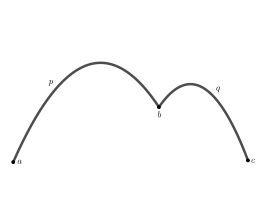
\includegraphics[width=\linewidth]{external/path_transitive.pdf}
\end{image}%
\tcblower
\end{figureptx}%
\begin{lemma}{Lemma}{The Gluing Lemma.}{}{lemma-sec_path_connect_equiv-d}%
\index{Gluing Lemma}%
Let \(A\) and \(B\) be closed subsets of a space \(X = A \cup B\), and let \(f:A \to Y\) and \(g: B \to Y\) be continuous functions into a space \(Y\) such that \(f(x)=g(x)\) for all \(x \in (A \cap B)\). Then the function \(h:X \to Y\) defined by%
\begin{equation*}
h(x) = \begin{cases}f(x) \amp \text{ if }  x \in A \\ g(x) \amp \text{ if }  x \in B \end{cases}
\end{equation*}
is continuous.%
\begin{figureptx}{Figure}{The Gluing Lemma.}{figure-F_Gluing_Lemma}{}%
\begin{image}{0.25}{0.5}{0.25}{}%
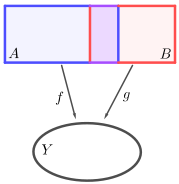
\includegraphics[width=\linewidth]{external/Gluing_Lemma.pdf}
\end{image}%
\tcblower
\end{figureptx}%
\end{lemma}
\begin{proof}{Proof}{}{proof-sec_path_connect_equiv-d-d}
Let \(A\) and \(B\) be closed subsets of a space \(X = A \cup B\), and let \(f:A \to Y\) and \(g: B \to Y\) be continuous functions into a space \(Y\) such that \(f(x)=g(x)\) for all \(x \in (A \cap B)\) as illustrated in \hyperref[figure-F_Gluing_Lemma]{Figure~{\xreffont\ref{figure-F_Gluing_Lemma}}}. Define \(h: X \to Y\) by%
\begin{equation*}
h(x) = \begin{cases}f(x) \amp \text{ if }  x \in A \\ g(x) \amp \text{ if }  x \in B. \end{cases}
\end{equation*}
%
\par
To show that \(h\) is continuous, let \(C\) be a closed subset of \(Y\). Then%
\begin{align*}
h^{-1}(C) = \{x \in X \mid h(x) \in C\} \amp = \{x \in A \mid f(x) \in C\} \cup \{x \in B \mid g(x) \in C\}\\
\amp = f^{-1}(C) \cup g^{-1}(C)\text{.}
\end{align*}
%
\par
Since \(f\) is continuous, \(f^{-1}(C)\) is closed in the subspace topology on \(A\) and since \(g\) is continuous \(g^{-1}(C)\) is closed in the subspace topology on \(B\). So \(f^{-1}(C) = A \cap D\) and \(g^{-1}(C) = B \cap E\) for some closed sets \(D\) and \(E\) of \(X\). The fact that \(A\) is closed in \(X\) implies that \(A \cap D\) is closed in \(X\). Similarly, the fact that \(B\) is closed in \(X\) implies that \(B \cap E\) is closed in \(X\). Thus,%
\begin{equation*}
h^{-1}(C) = f^{-1}(C) \cup g^{-1}(C) = (A \cap D) \cup (B \cap E)
\end{equation*}
is a finite union of closed sets in \(X\) and so is closed in \(X\). Since \(h^{-1}(C)\) is closed for every closed set in \(Y\), it follows that \(h\) is continuous.%
\end{proof}
We can use the Gluing Lemma to create a path from \(a\) to \(c\) given a path from \(a\) to \(b\) and a path from \(b\) to \(c\).%
\begin{activity}{Activity}{}{activity-sec_path_connect_equiv-f}%
Use the Gluing Lemma to explain why the path product given in the following definition is actually a path from \(p(0)\) to \(q(1)\).%
\begin{definition}{Definition}{}{definition-sec_path_connect_equiv-f-b}%
\index{path product}%
Let \(p\) be a path from \(a\) to \(b\) and \(q\) a path from \(b\) to \(c\) in a space \(X\). The \terminology{path product} \(q*p\) is the path in \(X\) defined by%
\begin{equation*}
(q*p)(x) = \begin{cases}p(2x) \amp \text{ for }  0 \leq x \leq \frac{1}{2} \\ q(2x-1) \amp \text{ for }  \frac{1}{2} \leq x \leq 1. \end{cases}
\end{equation*}
%
\end{definition}
\end{activity}%
Now we can show that path connectedness defines an equivalence relation on a topological space.%
\begin{activity}{Activity}{}{activity-sec_path_connect_equiv-h}%
Let \((X,\tau)\) be a topological space. Define a relation on \(X\) as follows:%
\begin{equation}
a \sim b \text{ if there is a path in }  X \text{ from }  a \text{ to }  b\text{.}\label{men-eq_path_equivalence}
\end{equation}
%
\begin{enumerate}[font=\bfseries,label=(\alph*),ref=\alph*]%
\item{}Explain why \(\sim\) is a reflexive relation.%
\item{}Explain why \(\sim\) is a symmetric relation.%
\item{}Explain why \(\sim\) is a transitive relation.%
\end{enumerate}%
\end{activity}%
Since \(\sim\) as defined in \hyperref[men-eq_path_equivalence]{({\xreffont\ref{men-eq_path_equivalence}})} is an equivalence relation, the relation partitions \(X\) into a union of disjoint equivalence classes. The equivalence class of an element \([a]\) is called a \terminology{path component} of \(X\), and is the largest path connected subset of \(X\) that contains \(a\).%
\begin{definition}{Definition}{}{definition-sec_path_connect_equiv-j}%
\index{path component}%
The \terminology{path component} of an element \(a\) in a topological space \((X, \tau)\) is the largest path connected subset of \(X\) that contains \(a\).%
\end{definition}
\end{sectionptx}
%
%
\typeout{************************************************}
\typeout{Section  Path Connectedness and Connectedness}
\typeout{************************************************}
%
\begin{sectionptx}{Section}{Path Connectedness and Connectedness}{}{Path Connectedness and Connectedness}{}{}{section-sec_connectedness}
Path connectedness and connectedness are different concepts, but they are related. In this section we will show that any path connected space must also be connected. We will see later that the converse is not true except in finite topological spaces.%
\begin{theorem}{Theorem}{}{}{theorem-thm_pctoc}%
If a topological space \(X\) is path connected, then \(X\) is connected.%
\end{theorem}
\begin{proof}{Proof}{}{proof-thm_pctoc-b}
Suppose that \(X\) is path connected. Let \(a \in X\) and for any \(x \in X\) let \(p_x\) be a path from \(a\) to \(x\). Let \(C_x = p_x([0,1])\). Now \(C_x\) is the continuous image of the connected set \([0,1]\) in \(\R\), so \(C_x\) is connected. Also, \(p_x(0) = a \in C_x\) and \(p_x(1) = x \in C_x\). Thus, every set \(C_x\) contains \(a\) and so \(\bigcap_{x \in X} C_x\) is not empty. Therefore,%
\begin{equation*}
C = \bigcup_{x \in X} C_x
\end{equation*}
is a connected subset of \(X\). But every \(x \in X\) is in a \(C_x\), so \(C = X\). We conclude that \(X\) is connected.%
\end{proof}
In the following sections we explore the reverse implication in \hyperref[theorem-thm_pctoc]{Theorem~{\xreffont\ref{theorem-thm_pctoc}}} \textemdash{} that is, does connectedness imply path connectedness.%
\end{sectionptx}
%
%
\typeout{************************************************}
\typeout{Section  Path Connectedness and Connectedness in Finite Topological Spaces}
\typeout{************************************************}
%
\begin{sectionptx}{Section}{Path Connectedness and Connectedness in Finite Topological Spaces}{}{Path Connectedness and Connectedness in Finite Topological Spaces}{}{}{section-sec_connect_finite}
In this section we will demonstrate that connectedness and path connectedness are equivalent concepts in finite topological spaces. In the following section, we prove that path connectedness and connectedness are not equivalent in infinite topological spaces. Throughout this section, we assume that \(X\) is a finite topological space. We begin with an example to motivate the main ideas.%
\begin{activity}{Activity}{}{activity-act_minimal_nbhds}%
Let \(X = \{a,b,c,d\}\) and \(\tau = \{\emptyset, \{b\}, \{c\}, \{a,b\}, \{b,c\}, \{a,b,c\}, \{b,c,d\}, X\}\). Assume that \(\tau\) is a topology on \(X\).%
\begin{enumerate}[font=\bfseries,label=(\alph*),ref=\alph*]%
\item{}Is \(X\) connected? Explain.%
\item{}For each \(x \in X\), let \(U_x\) be the intersection of all open sets that contain \(x\) (we call \(U_x\) a \terminology{minimal neighborhood} of \(x\)).%
\begin{definition}{Definition}{}{definition-def_min_nghb}%
\index{minimal neighborhood}%
For \(x \in X\), the \terminology{minimal neighborhood} \(U_x\) of \(x\) is the intersection of all open sets that contain \(x\).%
\end{definition}
Find \(U_x\) for each \(x \in X\).%
\item{}We will see that the minimal neighborhoods of \(X\) are path connected. Here we will illustrate with \(U_d\).%
\begin{enumerate}[font=\bfseries,label=(\roman*),ref=\theenumi.\roman*]%
\item{}Let \(p : [0,1] \to X\) be defined by%
\begin{equation*}
p(t) = \begin{cases}b \amp \text{ if }  0 \leq t \lt  \frac{1}{2} \\ d \amp \text{ if }  \frac{1}{2} \leq t \leq 1. \end{cases}
\end{equation*}
Show that \(p\) is a path in \(U_d\) from \(b\) to \(d\).%
\item{}Let \(p : [0,1] \to X\) be defined by%
\begin{equation*}
p(t) = \begin{cases}c \amp \text{ if }  0 \leq t \lt  \frac{1}{2} \\ d \amp \text{ if }  \frac{1}{2} \leq t \leq 1. \end{cases}
\end{equation*}
Show that \(p\) is a path in \(U_d\) from \(c\) to \(d\).%
\item{}Explain why \(U_d\) is path connected.%
\end{enumerate}%
\end{enumerate}%
\end{activity}%
The terminology in \hyperref[definition-def_min_nghb]{Definition~{\xreffont\ref{definition-def_min_nghb}}} is apt. Since every neighborhood \(N\) of a point \(x \in X\) must contain an open set \(O\) with \(x \in O\), it follows that \(U_x \subseteq O \subseteq N\). So every neighborhood of \(x \in X\) has \(U_x\) as a subset. In addition, when \(X\) is finite, the set \(U_x\) is a finite intersection of open sets, so the sets \(U_x\) are open sets (this is not true in general in infinite topological spaces \textemdash{} you are asked to find an example in \hyperlink{exercise-ex_U_x_not_open}{Exercise~{\xreffont 1}}). In \hyperref[activity-act_minimal_nbhds]{Activity~{\xreffont\ref{activity-act_minimal_nbhds}}} we saw that \(U_x\) was path connected for a particular \(x\) in one example. The next activity shows that this result is true in general in finite topological spaces.%
\begin{activity}{Activity}{}{activity-sec_connect_finite-e}%
Let \(X\) be a finite topological space, and let \(x \in X\). In this activity we demonstrate that \(U_x\) is path connected. Let \(y \in U_x\) and define \(p : [0,1] \to X\) by%
\begin{equation*}
p(t) = \begin{cases}y \amp \text{ if }  0 \leq t \lt  \frac{1}{2} \\ x \amp \text{ if }  \frac{1}{2} \leq t \leq 1. \end{cases}
\end{equation*}
%
\par
To prove that \(p\) is continuous, let \(O\) be an open set in \(X\). We either have \(x \in O\) or \(x \notin O\).%
\begin{enumerate}[font=\bfseries,label=(\alph*),ref=\alph*]%
\item{}Suppose \(x \in O\). Why must \(y\) also be in \(O\)? What, then, is \(p^{-1}(O)\)?%
\item{}Now suppose \(x \notin O\). There are two cases to consider.%
\begin{enumerate}[font=\bfseries,label=(\roman*),ref=\theenumi.\roman*]%
\item{}What is \(p^{-1}(O)\) if \(y \in O\)?%
\item{}What is \(p^{-1}(O)\) if \(y \notin O\)?%
\end{enumerate}%
\item{}Explain why \(p\) is a path from \(y\) to \(x\).%
\item{}Show that we can find a path between any two points in \(U_x\). Conclude that \(U_x\) is path connected.%
\end{enumerate}%
\end{activity}%
The sets \(U_x\) collectively form the space \(X\), and each of the \(U_x\) is a path connected subspace. So every point in \(X\) is contained in some neighborhood with a path connected subset containing \(x\). Spaces with this property are called \terminology{locally path connected}.%
\begin{definition}{Definition}{}{definition-sec_connect_finite-g}%
\index{path connected!locally}%
A topological space \((X, \tau)\) is \terminology{locally path connected at} \(x\) if every neighborhood of \(x\) contains a path connected open neighborhood with \(x\) as an element. The space \((X, \tau)\) is \terminology{locally path connected} if \(X\) is locally path connected at every point.%
\end{definition}
If \(X\) is a finite topological space, for any \(x \in X\) the set \(U_x\) is the smallest open set containing \(x\). This means that any neighborhood of \(N\) of \(x\) will contain \(U_x\) as a subset. Thus, a finite topological space is locally path connected (this is not true in general of infinite topological spaces, see \hyperlink{exercise-ex_PC_harmonic_broom}{Exercise~{\xreffont 4}} for example). One consequence of a locally path connected space is the following.%
\begin{lemma}{Lemma}{}{}{lemma-lem_open_PC}%
A space \(X\) is locally path connected if and only if for every open set \(O\) of \(X\), each path component of \(O\) is open in \(X\).%
\end{lemma}
\begin{proof}{Proof}{}{proof-lem_open_PC-b}
Let \(X\) be a locally path connected topological space. We first show that for every open set \(O\) in \(X\), every path component of \(O\) is open in \(X\). Let \(O\) be an open set in \(X\) and let \(P\) be a path component of \(O\). Let \(p \in P\). Since \(X\) is locally path connected, the neighborhood \(O\) of \(x\) contains an open path connected neighborhood \(Q\) of \(p\). The fact that \(p \in Q\) and \(P\) is a path component of \(O\) implies that \(Q \subseteq P\). Thus, \(P\) contains a neighborhood of \(p\) and \(P\) is open.%
\par
Now we show that if for every open set \(O\) in \(X\) the path components of \(O\) are open in \(X\), then \(X\) is locally path connected. Let \(x \in X\) and let \(N\) be a neighborhood of \(x\). Then \(N\) contains an open set \(U\) with \(x \in U\). Let \(P\) be the path component in \(U\) that contains \(x\). Now \(P\) is path connected and, by hypothesis, \(P\) is open in \(X\) and so is an open path connected neighborhood of \(x\). Thus, \(N\) contains a path connected neighborhood of \(x\) and \(X\) is locally path connected at every point.%
\end{proof}
Since \(X\) is open in \(X\) whenever \(X\) is a topological space, a natural corollary of \hyperref[lemma-lem_open_PC]{Lemma~{\xreffont\ref{lemma-lem_open_PC}}} is the following.%
\begin{corollary}{Corollary}{}{}{corollary-sec_connect_finite-k}%
Let \(X\) be a locally path connected topological space. Then every path component of \(X\) is open in \(X\).%
\end{corollary}
Since there are only finitely many open sets in the finite space \(X\), any arbitrary intersection of open sets in \(X\) just reduces to a finite intersection. So the intersection of any collection of open sets in \(X\) is again an open set in \(X\). We will show that \(X\) is a union of path connected components, which will ultimately allow us to prove that if \(X\) is connected, then \(X\) is also path connected.%
\begin{activity}{Activity}{}{activity-sec_connect_finite-m}%
Let \(X\) be a locally path connected topological space. In this activity we will prove that the components and path components of \(X\) are the same.%
\begin{enumerate}[font=\bfseries,label=(\alph*),ref=\alph*]%
\item{}Let \(x \in X\), and let \(C\) be the component of \(X\) containing \(x\) and \(P\) be the path component of \(X\) containing \(x\). Show that \(P \subseteq C\).%
\item{}To complete the proof that \(P = C\), proceed by contradiction and assume that \(C \neq P\). Let \(Q\) be the union of all path components of \(X\) that are different from \(P\) and that intersect \(C\). Each such path component is connected, and is therefore a subset of \(C\). So \(C = P \cup Q\). Explain why \(P\) and \(Q\) form a separation of \(C\).%
\par\smallskip%
\noindent\textbf{\blocktitlefont Hint}.\hypertarget{hint-sec_connect_finite-m-c-b}{}\quad{}How do we use the fact that \(X\) is locally path connected?%
\end{enumerate}%
\end{activity}%
We can now complete our main result of this section.%
\begin{theorem}{Theorem}{}{}{theorem-sec_connect_finite-o}%
Let \(X\) be a finite topological space. Then \(X\) is connected if and only if \(X\) is path connected.%
\end{theorem}
\begin{proof}{Proof}{}{proof-sec_connect_finite-o-b}
Let \(X\) be a finite topological space. \hyperref[theorem-thm_pctoc]{Theorem~{\xreffont\ref{theorem-thm_pctoc}}} demonstrates that if \(X\) is path connected, then \(X\) is connected. For the reverse implication, assume that \(X\) is path connected. Then \(X\) is composed of a single path component, \(P=X\). Since the path components and components of \(X\) are the same, we conclude that \(P= X\) is a component of \(X\) and that \(X\) is connected.%
\end{proof}
\end{sectionptx}
%
%
\typeout{************************************************}
\typeout{Section  Path Connectedness and Connectedness in Infinite Topological Spaces}
\typeout{************************************************}
%
\begin{sectionptx}{Section}{Path Connectedness and Connectedness in Infinite Topological Spaces}{}{Path Connectedness and Connectedness in Infinite Topological Spaces}{}{}{section-sec_connect_infinite}
\index{topologist's sine curve}%
Given that connectedness and path connectedness are equivalent in finite topological spaces, a reasonable question now is whether the converse of \hyperref[theorem-thm_pctoc]{Theorem~{\xreffont\ref{theorem-thm_pctoc}}} is true in arbitrary topological spaces. As we will see, the answer is no. To find a counterexample, we need to look in an infinite topological space. There are many examples, but a standard example to consider is the \terminology{topologist's sine curve}. This curve \(S\) is defined as the union of the sets%
\begin{equation*}
S_1 = \{(0,y) \mid -1 \leq y \leq 1\}  \ \text{ and }  \ S_2 = \left\{ \left(x,\sin\left(\frac{1}{x}\right)\right) \Big| \ 0 \lt  x \leq 1\right\}\text{.}
\end{equation*}
%
\par
A picture of \(S\) is shown in \hyperref[figure-F_T_sin]{Figure~{\xreffont\ref{figure-F_T_sin}}}.%
\begin{figureptx}{Figure}{The topologist's sine curve.}{figure-F_T_sin}{}%
\begin{image}{0.25}{0.5}{0.25}{}%
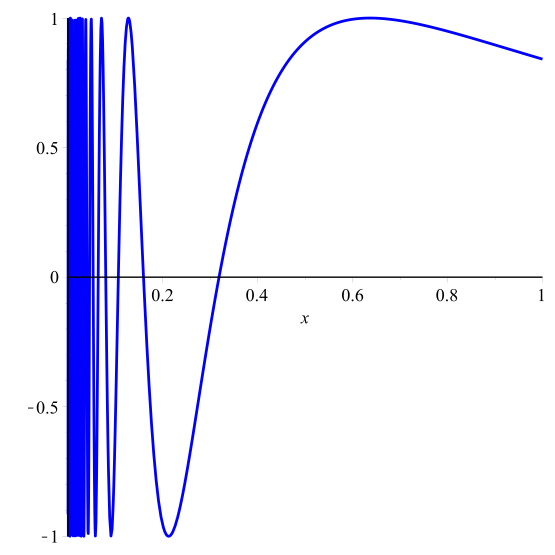
\includegraphics[width=\linewidth]{external/T_sin.pdf}
\end{image}%
\tcblower
\end{figureptx}%
To understand if \(S\) is connected, let us consider the relationship between \(S\) and \(S_2\). \hyperref[figure-F_T_sin]{Figure~{\xreffont\ref{figure-F_T_sin}}} seems to indicate that \(S = \overline{S_2}\). To see if this is true, let \(q=(0,y) \in S_1\), and let \(N\) be a neighborhood of \(q\). Then there is an \(\epsilon \gt 0\) such that \(B = B(q, \epsilon) \subseteq N\). Choose \(K \in \Z^+\) such that \(\frac{1}{\arcsin(y)+2 \pi K} \lt  \epsilon\), and let \(z = \frac{1}{\arcsin(y)+2 \pi K}\). Then%
\begin{align*}
d_E\left(q,\left(z, \sin\left(\frac{1}{z}\right)\right)\right) \amp =  d_E\left((0,y),(z, \sin(\arcsin(y)+2 \pi K)\right)\\
\amp = d_E((0,y), (z,\sin(\arcsin(y))))\\
\amp = d_E((0,y), (z,y))\\
\amp = \la z \ra\\
\amp \lt  \epsilon\text{,}
\end{align*}
and so \(\left(z, \arcsin(z)\right) \in B(q, \epsilon)\) and every neighborhood of \(q\) contains a point in \(S_2\). Therefore, \(S_1 \subseteq S_2' \subseteq \overline{S_2}\) and \(\overline{S_2} = S\) in \(S\). The fact that \(S\) is connected follows from \hyperref[theorem-thm_connected_limitpoints]{Theorem~{\xreffont\ref{theorem-thm_connected_limitpoints}}}.%
\par
Now that we know that \(S\) is connected, the following theorem demonstrates that \(S\) is a connected space that is not path connected.%
\begin{theorem}{Theorem}{}{}{theorem-sec_connect_infinite-h}%
The topologist's sine curve is connected but not path connected.%
\end{theorem}
\begin{proof}{Proof}{}{proof-sec_connect_infinite-h-b}
We know that \(S\) is connected, so it remains to show that \(S\) is not path connected. The sets \(S_1\) and \(S_2\) are connected (as continuous images of the interval \([0,1]\) and \((0,1]\), respectively). We will prove that there is no path \(p\) in \(S\) from \(p(0) = (0,0)\) to \(p(1) =  b\) for any point \(b \in S_2\) by contradiction. Assume the existence of such a path \(p\). Let \(U = p^{-1}(S_1)\) and \(V = p^{-1}(S_2)\). Then%
\begin{equation}
[0,1] = p^{-1}(S) = p^{-1}(S_1 \cup S_2) = p^{-1}(S_1) \cup p^{-1}(S_2) = U \cup V\text{.}\label{men-eq_TSC_1}
\end{equation}
%
\par
Note that \(S_2\) is an open subset of \(S\), since \(S_2 = \left( \bigcup_{z = (x,y) \in S_2} B\left(z, \frac{x}{2}\right)\right) \cap S\). So the continuity of \(p\) implies that \(V\) is an open subset of \([0,1]\). Also, the fact that \(p(0) \in S_1\) means that \(U \neq \emptyset\), and the fact that \(p(1) \in S_2\) means that \(V \neq \emptyset\). If we demonstrate that \(U\) is an open subset of \([0,1]\), then Equation \hyperref[men-eq_TSC_1]{({\xreffont\ref{men-eq_TSC_1}})} will imply that \([0,1]\) is not connected, a contradiction. So we proceed to prove that \(U\) is open in \([0,1]\).%
\par
Let \(x \in U\), and so \(p(x)\) in \(S_1\). The set \(O = B_S\left(p(x), \frac{1}{2}\right) \cap S\) is open in \(S\). The continuity of \(p\) then tells us that \(p^{-1}(O)\) is open in \([0,1]\). So there is a \(\delta \gt 0\) such that the open ball \(B=B_{[0,1]}(x, \delta)\) is a subset of \(p^{-1}(O)\). We will prove that \(p(B) \subseteq S_1\). This will imply that \(B \subseteq U\) and so \(U\) is a neighborhood of each of its points, and \(U\) is therefore an open set.%
\begin{figureptx}{Figure}{The set \(O\).}{figure-F_TSC_O}{}%
\begin{image}{0.25}{0.5}{0.25}{}%
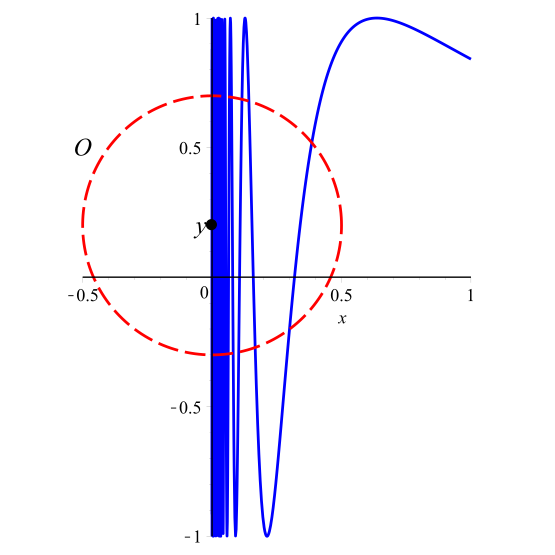
\includegraphics[width=\linewidth]{external/O_set.pdf}
\end{image}%
\tcblower
\end{figureptx}%
Every element in \(B\) is mapped into \(O\) by the path \(p\). The set \(O\) is complicated, consisting of infinitely many sub-curves of the curve \(S_2\), along with points in \(S_1\), as illustrated in \hyperref[figure-F_TSC_O]{Figure~{\xreffont\ref{figure-F_TSC_O}}}. To simplify our analysis, let us consider the projection onto the \(x\)-axis. The function \(P_x : \R^2 \to \R\) defined by \(P_x(x,y) = x\) is a continuous function. Let \(I = P_x(p(B))\). Since \(p(B) \subseteq O\), we know that \(I \subseteq P_x(O)\). Let \(Z = P_x(O)\). So \(I \subseteq Z\). Since \(B\) is a connected set (\(B\) is an interval), we know that \(p(B)\) is a connected set. The fact that \(P_x\) is continuous means that \(I = P_x(p(B))\) is connected as well. Now \(I\) is a bounded subset of \(\R\), so \(I\) must be a bounded interval. Recall that \(x \in B\) and so \(p(x) \in p(B)\). The fact that \(p(x) \in S_1\) tells us that \(0 = P_x(p(x)) \in P_x(p(B)) = I\). So \(I \neq \emptyset\). There are two possibilities for \(I\): either \(I = \{0\}\), or \(I\) is an interval of positive length. We consider the cases.%
\par
Suppose \(I = \{0\}\). Then the projection of \(p(B)\) onto the \(x\)-axis is the single point \(0\) and \(p(B) \subseteq S_1\) as desired. Suppose that \(I\) is an interval of the form \([0,d]\) or \([0,d)\) for some positive number \(d\). The structure of \(O\) would indicate that there must be some gaps in the set \(Z\), the projection of \(O\) onto the \(x\)-axis. This implies that \(I\) cannot be a connected interval. We proceed to show this. In other words, we will prove that \(I \setminus Z \neq \emptyset\) (which is impossible since \(I \subseteq Z\)). Remember that \(p(x) \in S_1\), so let \(p(x) = (0, q)\). We consider what happens if \(q \lt \frac{1}{2}\) and when \(q \geq \frac{1}{2}\).%
\par
Suppose \(q \lt \frac{1}{2}\). Then the ball \(B_S\left(p(x), \frac{1}{2}\right)\) contains only points with \(y\) value less than 1. Let \(N \in \Z^+\) so that \(t=\frac{1}{\pi/2+2N\pi} \lt d\). Then \(t \in I\). But \(\sin\left(\frac{1}{t}\right) = \sin(\pi/2 + 2N\pi) = \sin(\pi/2) = 1\), and so \(\left(t,\sin\left(\frac{1}{t}\right)\right)\) is not in \(O\). Thus, \(t \notin Z\). Thus we have found a point in \(I \setminus Z\).%
\par
Finally, suppose \(q \geq \frac{1}{2}\). Then the ball \(B_S\left(p(x), \frac{1}{2}\right)\) contains only points with \(y\) value greater than \(-1\). Let \(N \in \Z^+\) so that \(t=\frac{1}{3\pi/2+2N\pi} \lt d\). Then \(t \in I\). But \(\sin\left(\frac{1}{t}\right) = \sin(3\pi/2 + 2N\pi) = \sin(3\pi/2) = -1\), and so \(t \notin Z\). Thus we have found a point in \(I \setminus Z\).%
\par
We conclude that there can be no path in \(S\) from \((0,0)\) to any point in \(S_2\), completing our proof that \(S\) is not path connected. (In fact, the argument given shows that there is no path in \(S\) from any point in \(S_1\) to any point in \(S_2\).%
\end{proof}
\end{sectionptx}
%
%
\typeout{************************************************}
\typeout{Section  Summary}
\typeout{************************************************}
%
\begin{sectionptx}{Section}{Summary}{}{Summary}{}{}{section-sec_path_summ}
Important ideas that we discussed in this section include the following.%
\begin{itemize}[label=\textbullet]
\item{}A path in a topological space \(X\) is a continuous function \(p\) from the interval \([0,1]\) to \(X\). If \(p(0) = a\) and \(p(1) = b\), then \(p\) is a path from \(a\) to \(b\).%
\item{}A subspace \(A\) of a topological space \(X\) is path connected if, given any \(a,
b \in A\) there is a path in \(A\) from \(a\) to \(b\).%
\item{}The path component of an element \(a\) in a topological space \((X, \tau)\) is the largest path connected subset of \(X\) that contains \(a\).%
\item{}A topological space \((X, \tau)\) is locally path connected at \(x\) if every neighborhood of \(x\) contains a path connected subset with \(x\) as an element. The space \((X, \tau)\) is locally path connected if \(X\) is locally path connected at every point.%
\item{}Connectedness and path connectedness are equivalent in finite topological spaces, and path connectedness implies connectedness in general. However, there are topological spaces that are connected but not path connected. One example is the topologist's sine curve.%
\end{itemize}
%
\end{sectionptx}
%
%
\typeout{************************************************}
\typeout{Exercises  Exercises}
\typeout{************************************************}
%
\begin{exercises-section}{Exercises}{Exercises}{}{Exercises}{}{}{exercises-sec_path_exer}
\begin{divisionexercise}{1}{}{}{exercise-ex_U_x_not_open}%
Find a topological space \(X\) and a point \(x \in X\) such that the minimal neighborhood of \(x\) is not an open set.%
\end{divisionexercise}%
\begin{divisionexercise}{2}{}{}{exercise-sec_path_exer-b}%
Let \(X\) be a topological space and for each \(x \in X\) let \(PC(x)\) denote the path component of \(x\). Prove the following.%
\begin{enumerate}[font=\bfseries,label=(\alph*),ref=\alph*]%
\item{}If \(A\) is a path connected subset of \(X\), then \(A \subseteq PC(x)\) for some \(x \in X\).%
\item{}The space \(X\) is path connected if and only if \(X = PC(x)\) for some \(x \in X\).%
\end{enumerate}%
\end{divisionexercise}%
\begin{divisionexercise}{3}{}{}{exercise-sec_path_exer-c}%
In \hyperref[activity-act_connected_compenent]{Activity~{\xreffont\ref{activity-act_connected_compenent}}} of \hyperref[chapter-chap_Connected_topology]{Chapter~{\xreffont\ref{chapter-chap_Connected_topology}}} we showed that an arbitrary union of connected sets is connected provided the intersection of those sets is not empty. Is the same result true for path connected sets. That is, if \(X\) is a topological space and \(\{A_{\alpha}\}\) for \(\alpha\) in some indexing set \(I\) is a collection of path connected subsets of \(X\) and \(\bigcap_{\alpha \in I} A_{\alpha} \neq \emptyset\), must it be the case that \(A = \bigcup_{\alpha \in I} A_{\alpha}\) is path connected? Prove your answer.%
\end{divisionexercise}%
\begin{divisionexercise}{4}{}{}{exercise-ex_PC_harmonic_broom}%
Let \(X\) be the subspace of \((\R^2, d_E)\) consisting of the line segments joining the point \((0,1)\) to every point in the set \(\left\{\left(\frac{1}{n}, 0\right) \mid n \in \Z^+\right\}\) as illustrated in \hyperref[figure-F_harmonic_broom]{Figure~{\xreffont\ref{figure-F_harmonic_broom}}}. This space is called the \terminology{harmonic broom}.%
\begin{figureptx}{Figure}{The harmonic broom.}{figure-F_harmonic_broom}{}%
\begin{image}{0.25}{0.5}{0.25}{}%
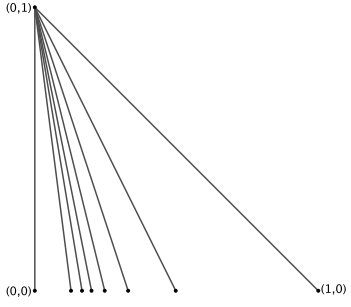
\includegraphics[width=\linewidth]{external/Harmonic_broom.pdf}
\end{image}%
\tcblower
\end{figureptx}%
\begin{enumerate}[font=\bfseries,label=(\alph*),ref=\alph*]%
\item{}Show that the harmonic broom is connected.%
\item{}Show that the harmonic broom is path connected.%
\item{}Show that the harmonic broom is not locally connected.%
\item{}Show that the harmonic broom is not locally path connected. So path connectedness does not imply local path connectedness.%
\end{enumerate}%
\end{divisionexercise}%
\begin{divisionexercise}{5}{}{}{exercise-sec_path_exer-e}%
In \hyperlink{exercise-ex_PC_harmonic_broom}{Exercise~{\xreffont 4}} we see an example of a space that is path connected but not locally path connected. Is it possible to find a space that is locally path connected but not path connected? Verify your answer.%
\end{divisionexercise}%
\begin{divisionexercise}{6}{}{}{exercise-sec_path_exer-f}%
Let  \(K = \left\{\frac{1}{k} \mid k \text{ is a positive integer} \right\}\). Let \(\B\) be the collection of all open intervals of the form \((a,b)\) and all sets of the form \((a,b) \setminus K\), where \(a \lt b\) are real numbers as in \hyperref[example-exp_K_topology]{Example~{\xreffont\ref{example-exp_K_topology}}}. Let \(\tau_K\) be the topology generated by \(\B\). Show that \((\R, \tau_K)\) is not path connected. (Hint: Suppose there is a path between \(a\) and \(b\) where \(a \lt 0\) and \(b \gt 1\).)%
\end{divisionexercise}%
\begin{divisionexercise}{7}{}{}{exercise-sec_path_exer-g}%
We know that a space can be connected but not path connected. We also know that local path connectedness does not imply connectedness. However, if we combine these conditions then a space must be path connected. That is, show that if a topological space \(X\) is connected and locally path connected, then \(X\) is path connected.%
\end{divisionexercise}%
\begin{divisionexercise}{8}{}{}{exercise-sec_path_exer-h}%
Let \(X\) be a nonempty set and let \(p\) be a fixed element in \(X\). Let \(\tau_p\) be the particular point topology and \(\tau_{\overline{p}}\) the excluded point topology on \(X\). That is%
\begin{itemize}[label=\textbullet]
\item{}\(\tau_{p}\) is the collection of subsets of \(X\) consisting of \(\emptyset\), \(X\), and all of the subsets of \(X\) that contain \(p\).%
\item{}\(\tau_{\overline{p}}\) is the collection of subsets of \(X\) consisting of \(\emptyset\), \(X\), and all of the subsets of \(X\) that do not contain \(p\).%
\end{itemize}
That the particular point and excluded point topologies are topologies is the subject of \hyperlink{exercise-ex_particular_point_topology}{Exercise~{\xreffont 9}} and \hyperlink{exercise-ex_excluded_point_topology}{Exercise~{\xreffont 10}}. Determine, with proof, the path connected subsets of \(X\) when%
\begin{enumerate}[font=\bfseries,label=(\alph*),ref=\alph*]%
\item{}\(X\) has the particular point topology \(\tau_p\)%
\item{}\(X\) has the excluded point topology \(\tau_{\overline{p}}\).%
\end{enumerate}%
\end{divisionexercise}%
\begin{divisionexercise}{9}{}{}{exercise-sec_path_exer-i}%
For each of the following, answer true if the statement is always true. If the statement is only sometimes true or never true, answer false and provide a concrete example to illustrate that the statement is false. If a statement is true, explain why.%
\begin{enumerate}[font=\bfseries,label=(\alph*),ref=\alph*]%
\item{}If \(X\) is a path connected topological space, then any subspace of \(X\) is path connected.%
\item{}If \(A\) and \(B\) are path connected subspaces of a topological space \(X\), then \(A \cap B\) is path connected.%
\item{}There is no path from \(a\) to \(b\) in \((X, \tau)\), where \(\tau\) is the discrete topology.%
\item{}If \(X\) is a compact locally path connected topological space, then \(X\) has only finitely many path components.%
\item{}Every locally path connected space is locally connected.%
\end{enumerate}%
\end{divisionexercise}%
\end{exercises-section}
\end{chapterptx}
 %
%
\typeout{************************************************}
\typeout{Chapter 20 Products of Topological Spaces}
\typeout{************************************************}
%
\begin{chapterptx}{Chapter}{Products of Topological Spaces}{}{Products of Topological Spaces}{}{}{chapter-chap_Product_topology}
\renewcommand*{\chaptername}{Chapter}
\begin{objectives}{Focus Questions}{objectives-chap_Product_topology-b}
%
\begin{itemize}[label=\textbullet]
\item{}What is the product of a finite number of topological spaces?%
\item{}How do we define a topology on the product of a finite number of topological spaces?%
\item{}What is a projection map from a product of a finite number of topological spaces?%
\item{}How can we use projection maps to determine the continuity of a function to a product of a finite number of topological spaces?%
\item{}What is a subbasis of a topological space?%
\item{}What properties do product spaces inherit from their factors?%
\end{itemize}
\end{objectives}
%
%
\typeout{************************************************}
\typeout{Section  Introduction}
\typeout{************************************************}
%
\begin{sectionptx}{Section}{Introduction}{}{Introduction}{}{}{section-sec_prod_top}
In \hyperref[chapter-chap_metric_subspaces]{Chapter~{\xreffont\ref{chapter-chap_metric_subspaces}}} we saw how we can make a Cartesian product of two metric spaces into a metric space. This is exactly the construction that allows us to work with the Cartesian plane \(\R^2\) as a metric space with the usual metric. As we discussed in \hyperref[chapter-chap_top_spaces]{Chapter~{\xreffont\ref{chapter-chap_top_spaces}}}, every metric space is a topological space, but not every topological space is metrizable. So knowing how to make a product of metric spaces into a metric space still leaves open the question of how we can make the product of topological spaces into a topological space. If we have two topological spaces \((X, \tau_X)\) and \((Y , \tau_Y)\), a natural approach to this problem might be to take as the open sets in \(X \times Y\) the sets of the form \(U \times V\) where \(U \in \tau_X\) and \(V \in \tau_Y\). We investigate this idea in \hyperref[exploration-PA_pd_top_1]{Preview Activity~{\xreffont\ref{exploration-PA_pd_top_1}}}.%
\begin{exploration}{Preview Activity}{}{exploration-PA_pd_top_1}%
Let \(X = \{a,b,c\}\) with \(\tau_X = \{\emptyset, \{a\}, \{b\}, \{a,b\}, \{a,c\}, X\}\), and let \(Y = \{1,2\}\) with \(\tau_Y = \{\emptyset, \{1\}, Y\}\).%
\begin{enumerate}[font=\bfseries,label=(\alph*),ref=\alph*]%
\item{}Let%
\begin{equation}
\CB = \{U \times V \mid U \in \tau_X \text{ and }  V \in \tau_Y\}\text{.}\label{men-eq_prod_basis}
\end{equation}
List all of the sets in \(\CB\) along with their elements.%
\item{}Assume that all of the sets in \(\CB\) are open sets in \(X \times Y\). Should the set \(A = \{(a,1), (a,2), (b,1)\}\) be an open set in \(X \times Y\)? Is the set \(A\) of the form \(U \times V\) for some open sets \(U\) in \(X\) and \(V\) in \(Y\)? Explain. Is \(\CB\) a topology on \(X \times Y\)?%
\item{}If \(\CB\) is not a topology on \(X \times Y\), what is the smallest collection of sets would we need to add to \(\CB\) to make a topology on \(X \times Y\)? Explain your process.%
\end{enumerate}%
\end{exploration}%
\end{sectionptx}
%
%
\typeout{************************************************}
\typeout{Section  The Topology on a Product of Topological Spaces}
\typeout{************************************************}
%
\begin{sectionptx}{Section}{The Topology on a Product of Topological Spaces}{}{The Topology on a Product of Topological Spaces}{}{}{section-sec_top_prod_space}
In our preview activity we learned that we cannot make a topology on a product \(X \times Y\) of topological spaces \((X, \tau_X)\) and \((Y , \tau_Y)\) with just the sets of the form \(U \times V\) where \(U \in \tau_X\) and \(V \in \tau_Y\) as the open sets since the collection of these sets is not closed under arbitrary unions. What we can do instead is consider these unions of all of the sets of the form \(U \times V\), where \(U\) is open in \(X\) and \(V\) is open in \(Y\). In other words, consider these sets to be a basis for the topology on \(X \times Y\).%
\begin{activity}{Activity}{}{activity-act_box_topology}%
Let \((X, \tau)\) and \((Y, \tau_Y)\) be topological spaces, and let \(\CB\) be as defined in \hyperref[men-eq_prod_basis]{({\xreffont\ref{men-eq_prod_basis}})}. Prove that \(\CB\) is a basis for a topology on \(X \times Y\).%
\end{activity}%
The argument from \hyperref[activity-act_box_topology]{Activity~{\xreffont\ref{activity-act_box_topology}}} can be extended to a product of any finite number of topological spaces. Let \(n\) be a positive integer and let \((X_i, \tau_i)\) be topological spaces for \(i\) from \(1\) to \(n\). Let%
\begin{equation*}
\CB = \left\{ \Pi_{i=1}^n O_i \mid O_i \text{ is open in }  X_i\right\}\text{.}
\end{equation*}
%
\par
Since \(X_i \in \tau_i\) for every \(i\), every point in \(\Pi_{i=1}^n X_i\) is in a set in \(\CB\). So \(\CB\) satisfies condition 1 of a basis. Now we show that \(\CB\) satisfies the second condition of a basis. Let \(B_1 = \Pi_{i=1}^n U_i\) and \(B_2 = \Pi_{i=1}^n V_i\) for some open sets \(U_i\), \(V_i\) in \(X_i\). Suppose \((x_i) \in (B_1 \cap B_2)\). Then for each \(j\) we have \(x_j \in U_j \cap V_j\) and so%
\begin{equation*}
(x_i) \in \Pi_{i=1}^n (U_i \cap V_i)\text{.}
\end{equation*}
%
\par
Since \(U_i \cap V_i\) is an open set in \(X_i\), it follows that \(\Pi_{i=1}^n (U_i \cap V_i)\) is in \(\CB\). Thus, \(\CB\) is a basis for a topology on \(X \times Y\).%
\par
This topology generated by products of open sets is called the \terminology{box} or \terminology{product} topology.%
\begin{definition}{Definition}{}{definition-def_box_topology}%
\index{box topology}%
\index{product topology}%
Let \((X_{\alpha}, \tau_{\alpha})\) be a collection of topological spaces for \(\alpha\) in some finite indexing set \(I\). The \terminology{box topology} or \terminology{product topology} on the product \(\Pi_{\alpha \in I} X_{\alpha}\) is the topology with basis%
\begin{equation*}
\CB = \left\{ \Pi_{\alpha \in I} U_{\alpha} \mid U_{\alpha} \in \tau_{\alpha}  \text{ for each }  \alpha \in I \right\}\text{.}
\end{equation*}
%
\end{definition}
So we can always make the product of topological spaces into a topological space using the box topology.%
\end{sectionptx}
%
%
\typeout{************************************************}
\typeout{Section  Three Examples}
\typeout{************************************************}
%
\begin{sectionptx}{Section}{Three Examples}{}{Three Examples}{}{}{section-sec_prod_top_exam}
In this section we consider three specific examples of a product of topological spaces.%
\begin{activity}{Activity}{}{activity-sec_prod_top_exam-c}%
Let \(X = [1,2]\) and \(Y = [3,4]\) as subspaces of \(\R^2\).%
\begin{enumerate}[font=\bfseries,label=(\alph*),ref=\alph*]%
\item{}Explain in detail what the product space \(X \times Y\) looks like.%
\item{}Find, if possible, an open subset of \(X \times Y\) that is not of the form \(U \times V\) where \(U\) is open in \(X\) and \(V\) is open in \(Y\).%
\end{enumerate}%
\end{activity}%
\begin{activity}{Activity}{}{activity-sec_prod_top_exam-d}%
Let \(X = \R\) and \(Y = S^1 = \{(x,y) \mid x^2 + y^2 = 1\}\), the unit circle as a subset of \(\R^2\).%
\begin{enumerate}[font=\bfseries,label=(\alph*),ref=\alph*]%
\item{}Draw a picture of \(\R\). For each \(x \in \R\), the set \(\R_x = \{(x, y) \mid y \in S^1\}\) is a subset of \(\R \times S^1\). On your graph of \(\R\), draw pictures of \(\R_x\) for \(x\) equal to \(-1\), \(0\), and \(1\). Explain in detail what the product space \(\R \times S^1\) looks like.%
\item{}Consider the sets of the form \(B \cap S^1\), where \(B\) is an open ball in \(\R^2\) (relatively open sets in \(S^1\)). What do these sets look like?%
\item{}Describe the shape of the basis elements for the product topology on \(\R \times S^1\) that result from products of the form \(U \times V\), where \(U\) is an open interval in \(\R\) and \(V\) is the intersections of \(S^1\) with an open ball in \(\R^2\).%
\end{enumerate}%
\end{activity}%
\begin{activity}{Activity}{}{activity-sec_prod_top_exam-e}%
Let \(2S^1 = \{(x,y) \mid x^2 + y^2 = 4\}\) be the circle of radius \(2\) centered at the origin as a subset of \(\R^2\). In this activity we investigate the space \(2S^1 \times S^1\).%
\begin{enumerate}[font=\bfseries,label=(\alph*),ref=\alph*]%
\item{}Draw a picture of \(2S^1\) in the \(xy\)-plane. For each \(p \in S^1\), the set \(S^1_p = \{(p, y) \mid y \in S^1\}\) is a subset of \(S^1 \times S^1\). On your graph of \(S^1\), draw pictures of \(S^1_p\) for \(p\) equal to \((1,0)\), \(\left(\frac{\sqrt{2}}{2}, \frac{\sqrt{2}}{2}\right)\), and \((0,1)\). Orient the graphs so that the copies of \(S^1\) are perpendicular to \(2S^1\). Explain in detail what the product space \(2S^1 \times S^1\) looks like.%
\item{}Consider the sets of the form \(B \cap S^1\), where \(B\) is an open ball in \(\R^2\). What do these sets look like?%
\item{}Describe the shape of the basis elements for the product topology on \(2S^1 \times S^1\) that result from products of the form \(U \times V\), where \(U\) and \(V\) are intersections of \(S^1\) with open balls in \(\R^2\).%
\end{enumerate}%
\end{activity}%
\end{sectionptx}
%
%
\typeout{************************************************}
\typeout{Section  Projections and Continuous Functions on Products}
\typeout{************************************************}
%
\begin{sectionptx}{Section}{Projections and Continuous Functions on Products}{}{Projections and Continuous Functions on Products}{}{}{section-sec_proj_cont_prod}
Given topological spaces \((X_1, \tau_1)\) and \((X_2, \tau_2)\), we define \(\pi_1: X_1 \times X_2 \to X_1\) and \(\pi_2: X_1 \times X_2 \to X_2\) by \(\pi_1((x,y)) = x\) and \(\pi_2((x,y)) = y\). These functions \(\pi_1\) and \(\pi_2\) are the \terminology{projections} \index{projection functions} of \(X_1 \times X_2\) onto \(X_1\) and \(X_2\), respectively. These projection functions can help us determine when a function \(f\) from a topological space \(Y\) to \(X_1 \times X_2\) is continuous.%
\begin{activity}{Activity}{}{activity-act_projection_continuous}%
Let \((X_1, \tau_1)\) and \((X_2, \tau_2)\) be topological spaces and let \(O_1\) be an open set in \(X_1\).%
\begin{enumerate}[font=\bfseries,label=(\alph*),ref=\alph*]%
\item{}Determine which set is \(\pi_1^{-1}(O_1)\). Verify your conjecture.%
\item{}Explain why \(\pi_1\) is continuous.%
\end{enumerate}%
\end{activity}%
The same argument as in \hyperref[activity-act_projection_continuous]{Activity~{\xreffont\ref{activity-act_projection_continuous}}} shows that \(\pi_2\) is also a continuous function. In general, if \(X = \Pi_{i=1}^n X_{i}\) is a finite product of topological spaces, then the projection \(\pi_{k}: X \to X_{k}\) is a continuous function for each \(k\), where \(\pi_k((x_1,x_2, \ldots, x_n)) = x_k\).%
\par
Let \(O = \Pi_{i=1}^n O_i\) be a basic open set in \(X = \Pi_{i=1}^n X_i\), where \(X_i\) is a topological space for each \(i\). We can extend the result of \hyperref[activity-act_projection_continuous]{Activity~{\xreffont\ref{activity-act_projection_continuous}}} to see that%
\begin{equation*}
\pi_i^{-1}(O_i) = X_1 \times X_2 \times \cdots \times X_{i-1} \times O_i \times X_{i+1} \times \cdots \times X_n\text{.}
\end{equation*}
%
\par
So%
\begin{equation*}
\Pi_{i=1}^n O_i = \bigcap_{i=1}^n \pi_i^{-1}(O_i)\text{.}
\end{equation*}
%
\par
So each basic open set is a finite intersection of sets of the form \(\pi_i^{-1}(O_i)\) where \(O_i\) is open in \(X_i\). When this happens, we call the collection of sets of the form \(\pi_i^{-1}(O_i)\) a \terminology{subbasis} of the topology.%
\begin{definition}{Definition}{}{definition-def_subbasis}%
\index{subbasis}%
\index{subbase}%
Let \((X, \tau)\) be a topological space. A subset \(\CS\) of \(\tau\) is a \terminology{subbasis} or \terminology{subbase} for \(\tau\) if the set of all finite intersections of elements of \(\CS\) is a basis for \(\tau\).%
\end{definition}
As an example, since finite intersections of intervals of the form \((-\infty,b)\) and \((a, \infty)\) give all intervals of the form \((a,b)\), the collection \(\CS = \{(-\infty,b), (a, \infty) \mid a, b \in \R\}\) is a subbasis for the standard topology on \(\R\). Note that this collection itself is not a basis for the standard topology on \(\R\). If \(X = \Pi_{i=1}^n X_i\) is a product of topological space, then another example of a subbasis is the collection%
\begin{equation*}
\CS = \bigcup_{i=1}^n \{\pi_i^{-1}(O_i) \mid O_i \text{ is open in }  X_i\}\text{.}
\end{equation*}
%
\par
This set is a subbasis for the product topology on \(X\) (the verification of this is left to \hyperlink{exercise-ex_subbasis}{Exercise~{\xreffont 1}}).%
\par
\index{product topology} We note here that there is another topology, called the \terminology{product topology}, on \(X\) with subbasis \(S = \bigcup_{\alpha \in I} S_{\alpha}\), where%
\begin{equation*}
S_{\alpha} = \{\pi_{\alpha}^{-1}(U_{\alpha}) \mid U_{\alpha} \text{ is open in } X_{\alpha}\}\text{.}
\end{equation*}
%
\par
For reasons we won't go into, the product topology is preferred to the box topology for infinite products (many important theorems that hold for finite products will not hold for infinite products using the box topology, but will hold using the product topology). However, the product topology and the box topology are the same for finite products, and since we won't consider infinite products here we will not worry about the distinction. For our purposes we will use the terms ``box topology'' and ``product topology'' interchangeably.%
\par
As we have discussed before, it can often be easier to define a topology using a basis or subbasis than it is to describe all of the sets in the topology. As we might expect, since the continuity of a function can be determined by the inverse image of basis elements, the continuity of a function can also be determined by the inverse image of subbasis elements.%
\begin{activity}{Activity}{}{activity-sec_proj_cont_prod-n}%
Prove \hyperref[theorem-thm_subbasis_continuous]{Theorem~{\xreffont\ref{theorem-thm_subbasis_continuous}}}.%
\begin{theorem}{Theorem}{}{}{theorem-thm_subbasis_continuous}%
Let \((X, \tau_X)\) and \((Y, \tau_Y)\) be topological spaces, let \(\CS\) be a subbasis for \(\tau_Y\), and let \(f: X \to Y\) be a function. If \(f^{-1}(S)\) is open in \(X\) for each \(S \in \CS\), then \(f\) is continuous.%
\end{theorem}
\par\smallskip%
\noindent\textbf{\blocktitlefont Hint}.\hypertarget{hint-sec_proj_cont_prod-n-b}{}\quad{}Recall that \(f\) is continuous if \(f^{-1}(B)\) is open in \(X\) for each basic open set \(B\).%
\end{activity}%
Now suppose that \(X_1\), \(X_2\), and \(Y\) are topological spaces, and that \(f: Y \to X_1 \times X_2\) is a function. Then \(\pi_1 \circ f\) maps \(Y\) to \(X_1\) and \(\pi_2 \circ f\) maps \(Y\) to \(X_2\). Since the composition of continuous functions is continuous, we can see that if \(f\) is continuous so are \(\pi_1\circ f\) and \(\pi_2 \circ f\). To determine if \(f\) is a continuous function, it would be useful to know if the converse is true. A key idea in the proof is the result of \hyperlink{exercise-ex_inverse_composite_sets}{Exercise~{\xreffont 9}} that if \(R\), \(S\), and \(T\) are sets, and \(g: R \to S\) and \(h : S \to T\) are functions, then \((h \circ g)^{-1}(O) = g^{-1}(h^{-1}(O)\) for any subset \(O\) of \(T\).%
\par
Now we can use projections to determine when functions to product spaces are continuous.%
\begin{theorem}{Theorem}{}{}{theorem-thm_prod_continuity}%
Let \(X_i\) for \(i\) from \(1\) to \(n\) and \(Y\) be topological spaces, and let \(f: Y \to \Pi_{i=1}^n X_i\) be a function. Then \(f\) is continuous if and only if \(\pi_i \circ f\) is continuous for each \(i\).%
\end{theorem}
\begin{proof}{Proof}{}{proof-thm_prod_continuity-b}
Let \(X_i\) for \(i\) from \(1\) to \(n\) and \(Y\) be topological spaces, and let \(f: Y \to \Pi X_i\) be a function. If \(f\) is continuous, the facts that each \(\pi_i\) is continuous and that composites of continuous functions are continuous show that \(\pi_i \circ f\) is continuous for each \(i\).%
\par
Now suppose that \(\pi_i \circ f\) is continuous for each \(i\). Recall that%
\begin{equation*}
\CS = \{\pi_i^{-1}(O_i) \mid O_i \text{ is open in }  X_i\}
\end{equation*}
is a subbasis for the product topology on \(\Pi_{i=1}^n X_i\). To prove that \(f\) is continuous, \hyperref[theorem-thm_subbasis_continuous]{Theorem~{\xreffont\ref{theorem-thm_subbasis_continuous}}} tells us that it is enough to show that \(f^{-1}(S)\) is open for each \(S\) in \(\CS\). Let \(O_i\) be an open set in \(X_i\). \hyperlink{exercise-ex_inverse_composite_sets}{Exercise~{\xreffont 9}} tells us that%
\begin{equation*}
f^{-1}(\pi_i^{-1}(O_i)) = (\pi_i \circ f)^{-1}(O_i)\text{,}
\end{equation*}
which is open in \(Y\) because \(\pi_i \circ f\) is continuous. Therefore, \(f\) is continuous.%
\end{proof}
\end{sectionptx}
%
%
\typeout{************************************************}
\typeout{Section  Properties of Products of Topological Spaces}
\typeout{************************************************}
%
\begin{sectionptx}{Section}{Properties of Products of Topological Spaces}{}{Properties of Products of Topological Spaces}{}{}{section-sec_prop_prod_top}
It is natural to ask what topological properties of the topological spaces \((X, \tau_X)\) and \((Y, \tau_Y)\) are inherited by the product \(X \times Y\). We have studied Hausdorff, connected, and compact spaces, and we now consider those properties.%
\begin{activity}{Activity}{}{activity-sec_prop_prod_top-c}%
Let \((X, \tau_X)\) and \((Y, \tau_Y)\) be Hausdorff spaces.%
\begin{enumerate}[font=\bfseries,label=(\alph*),ref=\alph*]%
\item{}What will it take to prove that the space \(X \times Y\) with the product topology is Hausdorff?%
\item{}Suppose that \((x_1,y_1), (x_2, y_2) \in X \times Y\). What does the fact that \(X\) is Hausdorff tell us about \(x_1\) and \(x_2\)? What can we say about \(y_1\) and \(y_2\)?%
\item{}Complete the proof of the following theorem.%
\begin{theorem}{Theorem}{}{}{theorem-sec_prop_prod_top-c-d-a-b}%
If \((X, \tau_X)\) and \((Y, \tau_Y)\) are Hausdorff spaces, then \(X \times Y\) with the product topology is a Hausdorff space.%
\end{theorem}
\end{enumerate}%
\end{activity}%
The proofs that a product of connected spaces is connected, that a product of path connected spaces is path connected, and that a product of compact spaces is compact are a bit more complicated. To prove that a product of two connected spaces is connected, we will use the result of \hyperref[activity-act_connected_compenent]{Activity~{\xreffont\ref{activity-act_connected_compenent}}} in \hyperref[chapter-chap_Connected_topology]{Chapter~{\xreffont\ref{chapter-chap_Connected_topology}}} that the union of connected subsets is connected if the intersection of the subsets is nonempty. A consequence of this result is the following.%
\begin{lemma}{Lemma}{}{}{lemma-lem_Connected_union}%
Let \(X\) be a topological space, and let \(A_{\alpha}\) be a connected subset of \(X\) for all \(\alpha\) in some indexing set \(I\). Let \(B\) be a connected subset of \(X\) such that \(A_{\alpha} \cap B \neq \emptyset\) for every \(\alpha \in I\). Then \(B \cup \left(\bigcup_{\alpha \in I} A_{\alpha} \right)\) is connected.%
\end{lemma}
\begin{proof}{Proof}{}{proof-lem_Connected_union-b}
Let \(X\) be a topological space, and let \(A_{\alpha}\) be a connected subset of \(X\) for all \(\alpha\) in some indexing set \(I\). Let \(B\) be a connected subset of \(X\) such that \(A_{\alpha} \cap B \neq \emptyset\) for every \(\alpha \in I\). For each \(\alpha \in I\) let \(B_{\alpha} = B \cup A_{\alpha}\). Let \(\beta \in I\). Since \(B \cap A_{\beta} \neq \emptyset\), \hyperref[lemma-lem_Connected_union]{Lemma~{\xreffont\ref{lemma-lem_Connected_union}}} shows that \(B_{\beta}\) is connected. Given that \(B\) is not empty, and \(B \subseteq \bigcap_{\alpha \in I} B_{\alpha}\), we see that \(\bigcap_{\alpha \in I} B_{\alpha} \neq \emptyset\). \hyperref[lemma-lem_Connected_union]{Lemma~{\xreffont\ref{lemma-lem_Connected_union}}} allows us to conclude that \(\bigcup_{\alpha \in I} B_{\alpha}\) is connected. But%
\begin{equation*}
\bigcup_{\alpha \in I} B_{\alpha} = \bigcup_{\alpha \in I} (B \cup A_{\alpha}) = B \cup \left(\bigcup_{\alpha \in I} A_{\alpha}\right)\text{,}
\end{equation*}
and so \(B \cup \left(\bigcup_{\alpha \in I} A_{\alpha}\right)\) is connected.%
\end{proof}
We will use \hyperref[lemma-lem_Connected_union]{Lemma~{\xreffont\ref{lemma-lem_Connected_union}}} to show that a product of connected spaces is connected.%
\begin{theorem}{Theorem}{}{}{theorem-thm_connected_product}%
If \((X, \tau_X)\) and \((Y, \tau_Y)\) are connected topological spaces, then \(X \times Y\) with the product topology is a connected topological space.%
\end{theorem}
\begin{proof}{Proof}{}{proof-thm_connected_product-b}
Assume \((X, \tau_X)\) and \((Y, \tau_Y)\) are connected topological spaces. Our approach to proving that \(X \times Y\) is connected is to write \(X \times Y\) as a union of two connected subspaces whose intersection is not empty. Let \(a \in X\). The space \(X_a = \{a\} \times Y\) is homeomorphic to \(Y\) via the inclusion map \(i\) which sends \((a,t) \in \{a\} \times Y\) to the point \(t \in Y\). Since \(Y\) is connected, so is \(X'\). Let \(b \in Y\). The space \(Y_b = X \times \{b\}\) is homeomorphic to \(X\) via the inclusion map \(i\) which sends \((s,b) \in X \times \{b\}\) to the point \(s \in X\). Since \(X\) is connected, so is \(Y_b\). (The verification of these homeomorphisms is left to the reader.) The point \((a,b)\) is in \(X_a \cap Y_b\), so \(X_a \cap Y_b \neq \emptyset\) for every \(b \in Y\). It follows that \(X_a \cup \left( \bigcup_{t \in Y} Y_t \right)\) is connected by \hyperref[lemma-lem_Connected_union]{Lemma~{\xreffont\ref{lemma-lem_Connected_union}}}. All that remains is to prove that \(X_a \cup \left( \bigcup_{t \in Y} Y_t \right) = X \times Y\) and we will have demonstrated that \(X \times Y\) is connected. The fact that \(X_a \subseteq X \times Y\) and \(Y_t \subseteq X \times Y\) for every \(t \in Y\) implies that \(X_a \cup \left( \bigcup_{t \in Y} Y_t \right) \subseteq X \times Y\). It then remains to show that \(X \times Y \subseteq X_a \cup \left( \bigcup_{t \in Y} Y_t \right)\). Let \((u,v) \in X \times Y\). Then \(u \in X\) and \(v \in Y\) and \((u,v) \in Y_v\). Thus, \(X \times Y \subseteq X_a \cup \left( \bigcup_{t \in Y} Y_t \right)\) and so \(X \times Y = X_a \cup \left( \bigcup_{t \in Y} Y_t \right)\). Therefore, \(X \times Y\) is connected.%
\end{proof}
Once we know that a product of connected topological spaces is connected, we can extend that result to any finite number of connected spaces by induction.%
\begin{corollary}{Corollary}{}{}{corollary-sec_prop_prod_top-i}%
Let \(X_{k}\) be a connected topological space for \(k\) from 1 to \(n\). Then the product \(\Pi_{k=1}^n X_k\) is connected.%
\end{corollary}
The proof is left to \hyperlink{exercise-ex_connected_product}{Exercise~{\xreffont 6}}.%
\par
We conclude this section by demonstrating that a product of compact topological spaces is compact. It is also true that finite products of path connected and compact spaces are path connected and compact. The proofs are left to \hyperlink{exercise-ex_compact_product}{Exercise~{\xreffont 7}} and \hyperlink{exercise-ex_path_connected_product}{Exercise~{\xreffont 8}}.%
\begin{theorem}{Theorem}{}{}{theorem-thm_compact_product}%
If \(X\) and \(Y\) are compact topological spaces, then \(X \times Y\) is a compact topological space under the product topology.%
\end{theorem}
\begin{proof}{Proof}{}{proof-thm_compact_product-b}
Let \((X, \tau_X)\) and \((Y, \tau_Y)\) be compact topological spaces. Let \(\CC = \{O_{\alpha}\}\) be an open cover of \(X \times Y\) for \(\alpha\) in some indexing set \(I\). Let \(a \in X\) and let \(Y_a = \{a\} \times Y\). Since \(Y_a\) is homeomorphic to \(Y\), we know that \(Y_a\) is compact. The collection \(\{O_{\alpha} \cap Y_a\}\) is an open cover of \(Y_a\), and so has a finite sub-cover \(\{O_{\alpha_i}\}_{1 \leq i \leq n}\). The set \(N_a = \bigcup_{1 \leq i \leq n} O_{\alpha_i}\) is an open set that contains \(Y_a\). We will show that there is a neighborhood \(W_a\) of \(a\) that \(N_a\) contains the entire set \(W_a \times Y\).%
\par
Cover the set \(Y_a\) with open sets that are contained in \(N_a\) (since \(N_a\) is open, we can intersect any open set with \(N_a\) and still have an open set). Each open set is a union of basis elements, so we can cover \(Y_a\) with basis elements \(U \times V\) that are contained in \(N_a\). Since \(Y_a\) is compact, there is a finite collection \(U_1 \times V_1\), \(U_2 \times V_2\), \(\ldots\), \(U_m \times V_m\) of basis elements contained in \(N_a\) that cover \(Y_a\). Assume that each \(U_i \times V_i\) intersects \(Y_a\) (otherwise, we can remove that set and still have a cover). Let \(W_a = U_1 \cap U_2 \cap \cdots \cap U_m\). Since \(a \in U_i\) for each \(i\), we know that \(W_a\) is not empty. Each \(U_i\) is open in \(X\) and so \(W_a\) is open in \(X\). Thus, \(W_a\) is a neighborhood of \(a\) in \(X\). Now we demonstrate that \(W_a \times Y \subseteq \bigcup_{1 \leq i \leq m} U_i \times V_i\). Let \((x,y) \in W_a \times Y\). Since the collection \(\{U_i \times V_i\}_{1 \leq i \leq m}\) covers \(Y_a\), the point \((a,y)\) is in \(U_k \times V_k\) for some \(k\) between \(1\) and \(m\). So \(y \in Y_k\). But \(x \in W_a = \bigcap_{1 \leq i \leq m} U_i\), so \(x \in U_k\). Thus, \((x,y) \in U_k \times V_k\) and we conclude that \(W_a \times Y \subseteq \bigcup_{1 \leq i \leq m} U_i \times V_i\).%
\par
So for each \(a \in X\), the set \(N_a\) contains a set of the form \(W_a \times Y\), where \(W_a\) is a neighborhood of \(a\) in \(X\). So \(W_a \times Y\) is covered by a finite sub-cover of our open cover \(\CC\) of \(X \times Y\). The collection \(\{W_a \times Y\}_{a \in X}\) is an open cover of \(X \times Y\). Since \(X\) is compact, the is a finite sub-cover \(W_1\), \(W_2\), \(\ldots\), \(W_r\) of the open cover \(\{W_a\}_{a \in X}\) of \(X\). is an open cover of \(X\). It follows that the sets \(W_1 \times Y\), \(W_2 \times Y\), \(\ldots\), \(W_r \times Y\) is a cover of \(X \times Y\). For each \(i\), the set \(W_i \times Y\) is covered by finitely many of the sets in \(\CC\), and so the collection of these sets forms a finite sub-cover of \(X \times Y\) in \(\CC\). Therefore, \(X \times Y\) is compact.%
\end{proof}
\end{sectionptx}
%
%
\typeout{************************************************}
\typeout{Section  Summary}
\typeout{************************************************}
%
\begin{sectionptx}{Section}{Summary}{}{Summary}{}{}{section-sec_prod_top_summ}
Important ideas that we discussed in this section include the following. Throughout, let \((X_i, \tau_i)\) be topological spaces for \(i\) from \(1\) to some integer \(n\)%
\begin{itemize}[label=\textbullet]
\item{}The product of the \(X_i\) is the Cartesian product \(\Pi_{i=1}^n X_i\).%
\item{}The set%
\begin{equation*}
\CB = \left\{ \Pi_{i=1}^n O_i \mid O_i \text{ is open in }  X_i\right\}
\end{equation*}
is a basis for the box topology on \(\Pi_{i=1}^n X_i\).%
\item{}The mapping \(\pi_j : \Pi_{i=1}^n X_i \to X_j\) defined by \(\pi_j((x_i)) = x_j\) is the projection map onto \(X_j\) for \(j\) from 1 to \(n\).%
\item{}A function \(f\) mapping a topological space \(Y\) to \(\Pi_{i=1}^n X_i\) is continuous if and only if \(\pi_j \circ f\) is continuous for every \(j\) from \(1\) to \(n\).%
\item{}Let \((X, \tau)\) be a topological space. A subset \(\CS\) of \(\tau\) is a subbasis for \(\tau\) if the set \(\CS\) of all finite intersections of elements of \(\CS\) is a basis for \(\tau\).%
\item{}If each \(X_i\) is (a) connected, (b) path connected, (c) compact, then \(\Pi_{i=1}^n X_i\) is (a) connected, (b) path connected, (c) compact with respect to the product topology.%
\end{itemize}
%
\end{sectionptx}
%
%
\typeout{************************************************}
\typeout{Exercises  Exercises}
\typeout{************************************************}
%
\begin{exercises-section}{Exercises}{Exercises}{}{Exercises}{}{}{exercises-sec_prod_top_exer}
\begin{divisionexercise}{1}{}{}{exercise-ex_subbasis}%
\begin{enumerate}[font=\bfseries,label=(\alph*),ref=\alph*]%
\item{}Let \((Y_1, \tau_1)\) and \((Y_2, \tau_2)\) be topological spaces, where \(Y_1 = \{a,b,c\}\) with \(\tau_1 = \{\emptyset, \{a\}, \{b,c\}, Y_1\}\) and \(Y_2 = \{1,2\}\) with \(\tau_2 = \{\emptyset, \{1\}, Y_2\}\). Find all of the sets of the form%
\begin{equation*}
\CS = \{\pi_1^{-1}(O_1) \mid O_1 \text{ is open in }  Y_1\} \cup \{\pi_2^{-1}(O_2) \mid O_2 \text{ is open in }  Y_2\}
\end{equation*}
and verify that these sets generate the product topology on \(Y_1 \times Y_2\).%
\item{}Let \(X_{i}\) for \(i\) from \(1\) to \(n\) be topological spaces and let \(X = \Pi_{i=1}^n X_i\). Show that the collection%
\begin{equation*}
\CS = \bigcup_{i=1}^n \{\pi_i^{-1}(O_i) \mid O_i \text{ is open in }  X_i\}
\end{equation*}
is a subbasis for the box topology on \(X\).%
\end{enumerate}%
\end{divisionexercise}%
\begin{divisionexercise}{2}{}{}{exercise-sec_prod_top_exer-b}%
Let \(X\) be the set of real numbers with the standard Euclidean metric topology and let \(Y\) be the real numbers with the discrete topology.%
\begin{enumerate}[font=\bfseries,label=(\alph*),ref=\alph*]%
\item{}Explain why the set of all ``horizontal intervals'' of the form%
\begin{equation*}
I= (a,b) \times \{c\} = \{(x,c) \mid a \lt  x \lt  b\}
\end{equation*}
is a base for the product topology on \(X \times Y\).%
\item{}Find the interior and closure of each of the following subsets of \(X \times Y\).%
\begin{enumerate}[font=\bfseries,label=(\roman*),ref=\theenumi.\roman*]%
\item{}\(A = \{(x,0) \mid 0 \leq x \lt 1\}\)%
\item{}\(B = \{(0,y) \mid 0 \leq y \lt 1\}\)%
\item{}\(C = \{(x,y) \mid 0 \leq x \lt 1, 0 \leq y \lt 1\}\)%
\end{enumerate}%
\end{enumerate}%
\end{divisionexercise}%
\begin{divisionexercise}{3}{}{}{exercise-ex_product_closure}%
Let \(X_1\) and \(X_2\) be topological space and let \(A_1\) be a subset of \(X_1\) and \(A_2\) a subset of \(X_2\). Assume the product topology on \(X_1 \times X_2\). Prove each of the following.%
\begin{enumerate}[font=\bfseries,label=(\alph*),ref=\alph*]%
\item{}\(\overline{A_1 \times A_2} = \overline{A_1} \times \overline{A_2}\)%
\item{}\(\Int(A_1 \times A_2) \subseteq \Int{A_1} \times \Int{A_2}\)%
\end{enumerate}%
\end{divisionexercise}%
\begin{divisionexercise}{4}{}{}{exercise-ex_unions_cross_products}%
Let \(X\) and \(Y\) be topological spaces and let \(\{U_{\alpha}\}_{\alpha \in I}\) and \(\{V_{\beta}\}_{\beta \in J}\) be collections of open sets in \(X\) and \(Y\), respectively, for some indexing sets \(I\) and \(J\). Show that%
\begin{equation*}
\bigcup_{\substack{\alpha \in I \\ \beta \in J} } (U_{\alpha} \times V_{\beta}) = \left(\bigcup_{\alpha \in I} U_{\alpha} \right) \times  \left(\bigcup_{\beta \in J} V_{\beta} \right)\text{.}
\end{equation*}
%
\end{divisionexercise}%
\begin{divisionexercise}{5}{}{}{exercise-sec_prod_top_exer-e}%
\begin{enumerate}[font=\bfseries,label=(\alph*),ref=\alph*]%
\item{}If \(S_1\), \(S_2\), \(T_1\), and \(T_2\) are sets, show that%
\begin{equation*}
(S_1 \times T_1) \cap (S_2 \times T_2) = (S_1 \cap S_2) \times (T_1 \cap T_2)\text{.}
\end{equation*}
%
\item{}If \(\CB_X\) is a base for a topology \(\tau_X\) on a space \(X\) and \(\CB_Y\) is a base for a topology \(\tau_Y\) on a space \(Y\), show that \(\CB_X \times \CB_Y\) is a base for the product topology on \(X \times Y\).%
\end{enumerate}%
\end{divisionexercise}%
\begin{divisionexercise}{6}{}{}{exercise-ex_connected_product}%
Prove that the product of any finite number of connected spaces is connected.%
\end{divisionexercise}%
\begin{divisionexercise}{7}{}{}{exercise-ex_compact_product}%
Prove that the product of any finite number of compact spaces is compact.%
\end{divisionexercise}%
\begin{divisionexercise}{8}{}{}{exercise-ex_path_connected_product}%
\begin{enumerate}[font=\bfseries,label=(\alph*),ref=\alph*]%
\item{}Prove that if \((X_1, \tau_1)\) and \((X_2, \tau_2)\) are path connected topological spaces, then \(X_1 \times X_2\) with the product topology is a path connected topological space.%
\item{}Prove that the product of any finite number of path connected spaces is path connected.%
\end{enumerate}%
\end{divisionexercise}%
\begin{divisionexercise}{9}{}{}{exercise-sec_prod_top_exer-i}%
Let \(X_1\) and \(X_2\) be topological spaces and \(X = X_1 \times X_2\). Is it true that if \(X\) is compact, then both \(X_1\) and \(X_2\) are compact. Prove your answer.%
\end{divisionexercise}%
\begin{divisionexercise}{10}{}{}{exercise-ex_projection_open}%
Let \(X_1\) and \(X_2\) be topological spaces and let \(\pi_i : X_1 \times X_2 \to X_i\) be the projection mapping. We have shown that \(\pi_i\) is continuous. Now show that \(\pi_i\) is an open map for \(i\) equal 1 and 2. Assume the standard product topology.%
\end{divisionexercise}%
\begin{divisionexercise}{11}{}{}{exercise-sec_prod_top_exer-k}%
Let \(X_1\) and \(X_2\) be topological spaces with cardinalities at least 2. Let \(X = X_1 \times X_2\). Prove that the product space topology on \(X = X_1 \times X_2\) is the discrete topology if and only if the topologies on \(X_1\) and \(X_2\) are the discrete topologies.%
\end{divisionexercise}%
\begin{divisionexercise}{12}{}{}{exercise-sec_prod_top_exer-l}%
For each of the following, answer true if the statement is always true. If the statement is only sometimes true or never true, answer false and provide a concrete example to illustrate that the statement is false. If a statement is true, explain why. Throughout, let \(X_1\) and \(X_2\) be topological spaces and \(X = X_1 \times X_2\) with the product topology.%
\begin{enumerate}[font=\bfseries,label=(\alph*),ref=\alph*]%
\item{}If \(A_1 \subseteq X_1\) and \(A_2 \subseteq X_2\), then \((X_1 \times X_2) \setminus (A_1 \times A_2) = (X_1 \setminus A_1) \times (X_2 \setminus A_2)\).%
\item{}If \(A_1 \subseteq X_1\) and \(A_2 \subseteq X_2\), then \(\Bdry(A_1 \times A_2) \subseteq \Bdry{A_1} \times \Bdry{A_2}\).%
\item{}If \(A_1 \subseteq X_1\) and \(A_2 \subseteq X_2\), then \(\Bdry{A_1} \times \Bdry{A_2} \subseteq \Bdry(A_1 \times A_2)\).%
\item{}If \(O_1\) is an open subset of \(X_1\) and \(O_2\) is an open subset of \(X_2\), then \(O_1 \times O_2\) is an open subset of \(X_1 \times X_2\).%
\item{}If \(O_1\) is a subset of \(X_1\) and \(O_2\) is a subset of \(X_2\) and \(O_1 \times O_2\) is an open subset of \(X_1 \times X_2\), then \(O_1\) is an open subset of \(X_1\) and \(O_2\) is an open subset of \(X_2\).%
\item{}If \(C_1\) is a closed subset of \(X_1\) and \(C_2\) is a closed subset of \(X_2\), then \(C_1 \times C_2\) is a closed subset of \(X_1 \times X_2\).%
\item{}If \(C_1\) is a subset of \(X_1\) and \(C_2\) is a subset of \(X_2\) and \(C_1 \times C_2\) is a closed subset of \(X_1 \times X_2\), then \(C_1\) is a closed subset of \(X_1\) and \(C_2\) is a closed subset of \(X_2\).%
\end{enumerate}%
\end{divisionexercise}%
\end{exercises-section}
%
%
\typeout{************************************************}
\typeout{Section  Applications of Products of Topological Spaces}
\typeout{************************************************}
%
\begin{sectionptx}{Section}{Applications of Products of Topological Spaces}{}{Applications of Products of Topological Spaces}{}{}{section-sec_prod_top_app}
Computers represent information from the real world digitally. That is, a computer screen consists of discrete pixels that are used to mimic the continuous information from the real world. So we exist in \(\R^3\), but a computer screen represents information in \(\Z^2\) as illustrated in \hyperref[figure-F_Digital_plane]{Figure~{\xreffont\ref{figure-F_Digital_plane}}}. It is important to be able to accurately mimic the continuous information from digital data. One of the key ideas is to have a digital version of the Jordan curve theorem which states that a Jordan curve (a continuous loop that does not intersect itself) in the Euclidean plane separates the remainder of the plane into two connected components (the inside and the outside of the curve). Additionally, if a single point is removed from a Jordan curve, the remainder of the plane becomes connected. The reason a digital Jordan curve theorem is important is that it is only necessary to save the Jordan curves which determine regions, along with the associated colors of the regions, rather than having to save the color of every single pixel in an image.%
\begin{figureptx}{Figure}{Left: The digital plane. Middle: \(4\)-neighbors of a point. Right: \(8\)-neighbors of a point.}{figure-F_Digital_plane}{}%
\begin{sidebyside}{3}{0.0166666666666667}{0.0166666666666667}{0.0333333333333333}%
\begin{sbspanel}{0.3}%
\includegraphics[width=\linewidth]{external/digital_grid.pdf}
\end{sbspanel}%
\begin{sbspanel}{0.3}%
\includegraphics[width=\linewidth]{external/neighbors_4.pdf}
\end{sbspanel}%
\begin{sbspanel}{0.3}%
\includegraphics[width=\linewidth]{external/neighbors_8.pdf}
\end{sbspanel}%
\end{sidebyside}%
\tcblower
\end{figureptx}%
A natural start to building a digital topology might be to identify neighborhoods. The idea of a neighborhood is to consider elements that are close to a point, and in the digital world there are different ways to do this. Given a point \((x,y)\) in \(\Z^2\), the 4-neighbors of \((x,y)\) are the points vertically or horizontally adjacent to \((x,y)\): that is, the points \((x \pm 1, y)\) and \((x, y \pm 1)\). The 8-neighbors of \((x,y)\) are the 4-neighbors along with the points diagonally adjacent to \((x,y)\): that is, \((x \pm 1, y)\), \((x, y \pm 1)\), \((x \pm 1, y \pm 1)\). These neighbors are illustrated in \hyperref[figure-F_Digital_plane]{Figure~{\xreffont\ref{figure-F_Digital_plane}}}, with the crosses indicating the neighbors of the highlighted point.%
\par
In the continuous case, we define a path between points to be a continuous function from \([0,1]\) to the space. However, we cannot have continuity in the digital world. So we define paths by moving through neighbor points. That is, if \(k\) is either \(4\) or \(8\), a \(k\)-path is a finite sequence \(p_0\), \(p_1\), \(\ldots\), \(p_m\) in \(\Z^2\) such that \(p_1\) is a \(k\)-neighbor of \(p_2\), \(p_2\) is a \(k\)-neighbor of \(p_3\), \(\ldots\), and \(p_{m-1}\) is a \(k\)-neighbor of \(p_m\).%
\begin{activity}{Activity}{}{activity-act_digital_graph_theory}%
\begin{enumerate}[font=\bfseries,label=(\alph*),ref=\alph*]%
\item{}Show that there is a \(4\)-path connecting any two points in \(\Z^2\). Then explain why there is an \(8\)-path connecting any two points in \(\Z^2\).%
\item{}In the continuous case, every Jordan curve separates \(\R^2\) into two connected regions. To have a similar theorem in the discrete case, we need a notion of connectedness in \(\Z^2\). Every image is made up of a finite number of pixels, and so we can think of a digital image as existing in a finite subspace of \(\Z^2\). Since connectedness and path connectedness are equivalent in finite topological spaces, we us the idea of \(k\)-paths to define connectedness in \(\Z^2\). We say that a subset \(S\) of \(\Z^2\) is \(k-connected\) if if any two of its points can be joined by a \(k\)-path in \(S\). \hyperref[figure-F_Digital_curves]{Figure~{\xreffont\ref{figure-F_Digital_curves}}} show two sets (curves) in the digital plane indicated by the points that connect the line segments (examples taken from A Topological Approach to Digital Topology, T. Yung Kong, R. Kopperman, and P. Meyer, \pubtitle{American Mathematical Monthly}, 98 (1991), no. 10, 901-917). Let \(S_1\) be the set illustrated at left in \hyperref[figure-F_Digital_curves]{Figure~{\xreffont\ref{figure-F_Digital_curves}}} and \(S_2\) the set at right.%
\begin{figureptx}{Figure}{Sets \(S_1\) (left) and \(S_2\) (right) in the digital plane.}{figure-F_Digital_curves}{}%
\begin{sidebyside}{2}{0.025}{0.025}{0.05}%
\begin{sbspanel}{0.45}%
\includegraphics[width=\linewidth]{external/digital_curve_1.pdf}
\end{sbspanel}%
\begin{sbspanel}{0.45}%
\includegraphics[width=\linewidth]{external/digital_curve_2.pdf}
\end{sbspanel}%
\end{sidebyside}%
\tcblower
\end{figureptx}%
Is \(S_1\) \(4\) connected? Is \(S_1\) \(8\) connected? Verify your answer. Repeat with \(S_2\).%
\item{}We can now define a Jordan \(k\)-curve to be a finite \(k\)-connected set which contains exactly two \(k\)-neighbors for each of its points. Is \(S_1\) a Jordan \(4\)-curve? Is \(S_1\) a Jordan \(8\)-curve? Verify your answer. Repeat with \(S_2\).%
\item{}As usual, we define a component to be a maximal connected set. Explain why \(S_1\) is a Jordan \(8\)-curve whose complement is connected and why \(S_2\) is a Jordan \(4\)-curve whose complement consists of three connected \(4\)-components. This example shows that there is no Jordan curve theorem in digital topology using the standard notions of \(k\)-connectedness with \(k\) either \(4\) or \(8\). So neither 4-adjacency nor 8-adjacency provides an analogue of the Jordan curve theorem and it is necessary to use a combination of both. That is, a Jordan \(4\)-curve with at least five points separates \(\Z^2\) into exactly two \(8\)-components, and a Jordan \(8\)-curve with at least five points separates \(\Z^2\) into exactly two \(4\)-components.%
\end{enumerate}%
\end{activity}%
In \hyperref[activity-act_digital_graph_theory]{Activity~{\xreffont\ref{activity-act_digital_graph_theory}}} we discussed the importance of a digital Jordan curve theorem. In the next activity we describe a topology in which such a theorem exists.%
\begin{activity}{Activity}{}{activity-act_digital_Jordan_curve}%
\index{topology!Khalimsky}%
Consider \(Z\) with the topology \(\tau_1\) with basis \(\{B(n)\}\), where%
\begin{equation*}
B(n) = \begin{cases}\{n\}  \amp \text{ if \(n\) is odd } , \\ \{n-1,n,n+1\}  \amp \text{ if \(n\) is even } . \end{cases}
\end{equation*}
%
\par
This topology is called the \terminology{digital line topology} or the \terminology{Khalimsky topology} on \(\Z\). Notice that all sets of the form \(\{n\}\) are open when \(n\) is odd.%
\begin{enumerate}[font=\bfseries,label=(\alph*),ref=\alph*]%
\item{}Show that any set of the form \(\{n\}\) where \(n\) is even is closed in the digital line topology.%
\item{}To define a \terminology{Khalimsky topology} on \(\Z^2\) we use the product topology. Explain why the collection of sets \(\{B(m,n)\}\) where%
\begin{equation*}
B(m,n) = \begin{cases}\{(m,n)\}  \amp  m \text{ and }  n \text{ odd, }  \\ \{(m-i,n-j) \mid -1 \leq i \leq 1, -1 \leq j \leq 1\} \amp m \text{ and }  n \text{ even, }  \\ \{(m,n-1), (m,n), (m,n+1)\} \amp m \text{ odd and }  n \text{ even, }  \\ \{(m-1,n), (m,n), (m+1,n)\} \amp m \text{ even and }  n \text{ odd } \end{cases}
\end{equation*}
is a basis for the Khalimsky topology \(\tau_2\) on \(\Z^2\). (This topology was originally published by E. Khalimsky in \pubtitle{Applications of connected ordered topological spaces in topology}, Conference of math. departments of Povolsia, 1970.)%
\item{}Now we want to define a digital Jordan curve. Our first step is to define a \terminology{digital path}. Recall that a path in a topological space is a homeomorphism from the interval \([0,1]\) into the space. So we need the concept of a digital interval. If \(z_1 \lt  z_2\) in \((\Z, \tau_1)\), the \terminology{digital interval} \([z_1,z_2]\) is the set%
\begin{equation*}
[z_1, z_2] = \{z \in \Z \mid z_1 \leq z \leq z_2\}\text{.}
\end{equation*}
%
\par
The integers \(z_1\) and \(z_2\) are called the \terminology{endpoints} of the digital interval \([z_1,z_2]\).%
\begin{definition}{Definition}{}{definition-act_digital_Jordan_curve-e-a-c}%
\index{digital path}%
\index{digital arc}%
Let \(X\) be a topological space.%
\begin{itemize}[label=\textbullet]
\item{}A \terminology{digital path} in \(X\) is the range of a continuous function from a digital interval to \(X\).%
\item{}A \terminology{digital arc} in X is the range of a homeomorphism from a digital interval to \(X\).%
\end{itemize}
%
\end{definition}
Let%
\begin{align*}
S_1 \amp = \{(1,-1), (1,1), (-1,1), (-1,-1)\},\\
S_2 \amp = \{(0,0), (1,-1), (2,0), (1,1)\}, \text{ and }\\
S_3 \amp = \{(1,-1), (1,0), (1,1), (0,1), (-1,1), (-1,0), (-1,-1), (0,-1)\}\text{.}
\end{align*}
Show that \(S_1\) is not a digital path but \(S_2\) and \(S_3\) are digital paths.%
\item{}To produce a digital Jordan Curve Theorem, we need a definition of a digital Jordan curve.%
\begin{definition}{Definition}{}{definition-act_digital_Jordan_curve-f-a-b}%
\index{digital Jordan curve}%
A \terminology{digital Jordan curve} is a finite connected set \(J\) with \(|J| \geq 4\) such that \(J \setminus \{j\}\) is a digital arc for each \(j \in J\).%
\par
So every digital Jordan curve is a connected set. Show that any finite digital path in \(\Z^2\) is a connected set.%
\end{definition}
\par\smallskip%
\noindent\textbf{\blocktitlefont Hint}.\hypertarget{hint-act_digital_Jordan_curve-f-b}{}\quad{}Is every digital interval connected?%
\item{}The upshot of all of this is the following theorem (a proof can be found in A Topological Approach to Digital Topology, T. Yung Kong, R. Kopperman, and P. Meyer, \pubtitle{American Mathematical Monthly}, 98 (1991), no. 10, 901-917).%
\begin{theorem}{Theorem}{}{}{theorem-thm_digital_Jordan_curve}%
If \(J\) is a digital Jordan curve in the digital plane \(\Z^2\), then \(\Z^2 \setminus J\) has exactly two components.%
\end{theorem}
The two components in \hyperref[theorem-thm_digital_Jordan_curve]{Theorem~{\xreffont\ref{theorem-thm_digital_Jordan_curve}}} split the digital plane into an infinite region (the outside) and a finite region (the inside).%
\par
Show that \(S_2\) is a digital Jordan curve (and thus splits \(\Z^2\) into two connected components).%
\end{enumerate}%
\end{activity}%
Digital Jordan curves, as described in \hyperref[activity-act_digital_Jordan_curve]{Activity~{\xreffont\ref{activity-act_digital_Jordan_curve}}}, are important in order to have a digital Jordan curve theorem. Christer O. Kiselman presents the following theorem to characterize digital Jordan curves in \pubtitle{Discrete Geometry for Computer Imagery}, Springer-Verlag, 2000, p. 46-56.%
\begin{theorem}{Theorem}{}{}{theorem-thm_digital_curve}%
A subset \(J\) of \(\Z^2\) equipped with the Khalimsky topology is a digital Jordan curve if and only if \(J = \{P_1, P_2, \ldots, P_m\}\) for some even integer \(m \geq 4\) and for all \(j\), \(P_{j?1}\) and \(P_{j+1}\) and no other points are adjacent to \(P_j\); moreover each path consisting of three consecutive points \(P_{i?1}\), \(P_i\), \(P_{i+1}\) turns at \(P_i\) by \(45^{\circ}\) or \(90^{\circ}\) or not at all if \(P_i\) is a pure point, and goes straight ahead if \(P_i\) is mixed.%
\end{theorem}
We investigate this theorem in the next activity.%
\begin{activity}{Activity}{}{activity-sec_prod_top_app-l}%
\begin{enumerate}[font=\bfseries,label=(\alph*),ref=\alph*]%
\item{}We need to first define the appropriate terms. Let \(X\) be a topological space. Two points \(x\) and \(y\) in \(X\) are \terminology{adjacent} if \(x \neq y\) and the set \(\{x, y\}\) is connected. Then let \(N(x)\) to be the intersection of all neighborhoods of \(x\). Show that distinct elements \(x\) and \(y\) in a topological space \(X\) are adjacent if and only if \(x \in N(y)\) or \(y \in N(x)\).%
\item{}A point \((x_1,x_2)\) in \(\Z^2\) is called \terminology{pure} if \(x_1\) and \(x_2\) have the same parity. Otherwise, the point is \terminology{mixed}. Find \(N(P)\) if \(P\) is a pure point or a mixed point.%
\item{}In \hyperref[activity-act_digital_Jordan_curve]{Activity~{\xreffont\ref{activity-act_digital_Jordan_curve}}} we show that the set \(S_1 = \{(1,-1), (1,1), (-1,1), (-1,-1)\}\) is not a digital path and so not a digital Jordan curve. Which part of \hyperref[theorem-thm_digital_curve]{Theorem~{\xreffont\ref{theorem-thm_digital_curve}}} does \(S_1\) violate?%
\item{}In \hyperref[activity-act_digital_Jordan_curve]{Activity~{\xreffont\ref{activity-act_digital_Jordan_curve}}} we show that the set \(S_2 = \{(0,0), (1,-1), (2,0), (1,1)\}\) is a digital Jordan curve. Show that in \(S_2\), the property from \hyperref[theorem-thm_digital_curve]{Theorem~{\xreffont\ref{theorem-thm_digital_curve}}} that \(x_{j-1}\) and \(x_{j+1}\) and no other points are adjacent to \(x_j\) is satisfied for each \(j\).%
\end{enumerate}%
\end{activity}%
\end{sectionptx}
\end{chapterptx}
\end{partptx}
%
\backmatter%
%
\clearpage\phantomsection%
\addcontentsline{toc}{part}{Back Matter}%
%
%% The index is here, setup is all in preamble
%% Index locators are cross-references, so same font here
{\xreffont\printindex}
%
\end{document}
